

\documentclass[11pt]{article}

%%%% DEPENDENCIES v1.8 %%%%%%

\usepackage{graphicx}
\usepackage[backend=bibtex,style=numeric,natbib=true,citestyle=numeric,sorting=none]{biblatex}
\synctex=1


\usepackage{amsthm}
\usepackage{amsfonts}
\usepackage{mathtools}
%\usepackage{enumerate}
\usepackage{enumitem}
\usepackage[section]{placeins}

\setlength {\marginparwidth }{2cm}
\usepackage{todonotes}
\usepackage{esint}
\usepackage{float}
%
%\usepackage{mathrsfs}

\usepackage{hyperref}
\hypersetup{
    colorlinks=true, %set true if you want colored links
    linktoc=all,     %set to all if you want both sections and subsections linked
    linkcolor=blue,  %choose some color if you want links to stand out
}
\hypersetup{linktocpage}
\DeclareUnicodeCharacter{0301}{\'{e}}

% inscape-figures
%\usepackage{import}
%\usepackage{pdfpages}
%\usepackage{transparent}
% \usepackage{xcolor}
%\newcommand{\incfig}[2][1]{%
%\def\svgwidth{#1\columnwidth}
%\import{./figures/}{#2.pdf_tex} } \pdfsuppresswarningpagegroup=1

% Box environment
\usepackage{tcolorbox}
\usepackage{mdframed}

% \newmdtheoremenv{definition}{Definition}[section]
\newmdtheoremenv{theorem}{Theorem}[section]
\newtheorem{definition}[theorem]{Definition}
\newtheorem{problem}[theorem]{Problem}
\newtheorem{assumption}{Assumption}
\newtheorem*{assumption*}{Assumption} % unnumbered
\newtheorem{corollary}[theorem]{Corollary}
\newtheorem{proposition}[theorem]{Proposition}
\newtheorem{lemma}[theorem]{Lemma}

\DeclareMathOperator{\atantwo}{atan2}
\DeclareMathOperator{\arctantwo}{arctan2}

\theoremstyle{remark}
\newtheorem*{remark}{Remark}
%\newtheorem{example}{Example}

\newcommand{\newpara}
    {
    \vskip 0.4cm
    }

\newcommand\Item[1][]{%
  \ifx\relax#1\relax  \item \else \item[#1] \fi
  \abovedisplayskip=0pt\abovedisplayshortskip=0pt~\vspace*{-\baselineskip}}

\newcommand{\mean}[1]{\left\{\!\!\left\{#1\right\}\!\!\right\}}
\newcommand{\jump}[1]{\left[\!\left[ #1 \right]\!\right]}
\newcommand{\abs}[1]{\left\lvert #1 \right\rvert}
\newcommand{\red}[1]{\textcolor{red}{ #1 }}
\let\oldleq\le
\renewcommand{\le}{\leqslant}
\let\oldgeq\ge
\renewcommand{\ge}{\geqslant}

\usepackage{geometry}
%\usepackage{showframe} %This line can be used to clearly show the new margins

\newgeometry{vmargin={15mm}, hmargin={15mm,37mm}}

\usepackage{amsmath}
\numberwithin{equation}{section}
\usepackage{amssymb}
\usepackage{subfig}

% \usepackage{subcaption} % cannot be used with subfig
%\subcaption -> \subfloat[Laplace]{\input{ex.tex}}
% \usepackage{newtxmath}
% \usepackage{mwe}


\addbibresource{bibliography.bib} % Makes the bibliography file available to biblatex.
\addbibresource{biharmonic.bib} % Makes the bibliography file available to biblatex.

%% PGF PLOTS DEPENDECIES
\usepackage{pgfplots}
\usetikzlibrary{calc}
\usepgfplotslibrary{patchplots}
\usepgfplotslibrary{fillbetween}
\usetikzlibrary{arrows.meta}
\usetikzlibrary{backgrounds}
\pgfplotsset{compat=newest} % Set the compatibility mode for pgfplots

\pgfplotsset{%
    layers/standard/.define layer set={%
        background,axis background,axis grid,axis ticks,axis lines,axis tick labels,pre main,main,axis descriptions,axis foreground%
    }{
        grid style={/pgfplots/on layer=axis grid},%
        tick style={/pgfplots/on layer=axis ticks},%
        axis line style={/pgfplots/on layer=axis lines},%
        label style={/pgfplots/on layer=axis descriptions},%
        legend style={/pgfplots/on layer=axis descriptions},%
        title style={/pgfplots/on layer=axis descriptions},%
        colorbar style={/pgfplots/on layer=axis descriptions},%
        ticklabel style={/pgfplots/on layer=axis tick labels},%
        axis background@ style={/pgfplots/on layer=axis background},%
        3d box foreground style={/pgfplots/on layer=axis foreground},%
    },
}
%%%

% \usepackage{amsmath} % Required for the \Vert command%%%%%%%%%%%%%%%%%%%%%%%%%%%%%%%%%%%%%%%%%%%%%%%%%%%%%%%%%%%%

%
\newgeometry{vmargin={15mm}, hmargin={25mm,27mm}}
\usepackage{pdfpages}
\usepackage[utf8]{inputenc} % For utf8 input
\usepackage[T1]{fontenc} % For T1 encoding

\begin{document}

    \includepdf[pages=-]{results/illustration/front_page.pdf}

    \newpage


    \tableofcontents
    % \section{Introduction}\label{sec:introduction}

Cell membranes are the foundation of the origin of life, but also linked to the dynamics of virus al infections and genetic mutations since it controls what substances that can exit or enter the cell \cite{ hurley2010membrane}. In fact, a good
understanding of the cell membrane is important of engineering proteins to manipulate various intracellular processes in living systems \cite{rojas1998genetic}.

One of the primary components of the cell membranes are lipids which serve many different functions. A key function is that it is consisting of a bilayer of lipids which controls the structural rigidity and the fluidity of the membrane. Thus, elastic
bending forces, temperature and diffusion is essential on how a cell membrane will evolve \cite{udo97,neidleman87}.


\subsection{Elastic bending energy on evolving surfaces}%
\label{sub:willmore_flow}

Assuming that the system is a single-phase system, i.e., the lipids are uniformly distributed, can the elastic bending energy be modelled using the Canham-Helrich energy functional \cite{helfrich1973elastic, wang08, udo97}. Let us denote $b_{b},
b_{k}$ and $H_{0}$ as parameters based on physical models, then can the energy functional be denoted as,
\begin{equation}
\label{eq:CH}
\mathcal{E} _{CH}\left( \Gamma\left( t \right)   \right) =   \int_{\Gamma  }^{}  b_{b} \left( H- H_{0} \right) ^{2} + b_{k} K
.\end{equation}
Here is $H =  \kappa_1 + \kappa_2 $ denoted as the mean curvature and $K = \kappa_1 \kappa_2$ as the gaussian curvature with respectively and $\kappa_1$ and $\kappa_2$ as principal curvatures. $\Gamma \left( t
\right) = \Gamma  $ is here an evolving surface in $\mathbb{R} ^3$, for more info see section \ref{sec:background}.  Using the Gauss-Bonnet theorem can it be shown that the problem above is equivalent to the so-called Willmore energy
functional \cite{montiel2009curves, willmore1996riemannian},

\begin{equation}
\label{eq:WE}
\mathcal{E} _{W} \left( \Gamma\left( t \right)   \right) = \int_{\Gamma  }^{} \frac{1}{2} H ^2
.\end{equation}

This is a well known problem in the mathematical community \cite{ topping2000towards, marques2014willmore,link2013gradient,kuwert2012willmore}. In fact, it is a mathematical tool used to study the geometry of surfaces because it can be used to study
the diffeomorphism from a initial surface to a minimal energy configuration, which are surfaces with the least possible area for a given boundary. This is important in many areas of mathematics, including differential geometry, topology and mathematical physics \cite{koerber2021area,jakob2022singularities, rupp21}.

It has been established many numerical methods for for shape optimization problems \cite{sokolowski1992introduction,ito2008variational}, evolving surface partial differential equations (PDE) \cite{dziuk2013finite, dziuk2007finite,
binz2022convergent, barrett2007parametric, barrett2007variational, kovacs2019convergent, lehrenfeld2018stabilized} and specific
algorithms for the Willmore energy problem \eqref{eq:WE} \cite{palmurella2022parametric, dziuk2008computational, bonito2010parametric,  kovacs2021convergent, hu2022evolving}.

\subsection{Two-phase separation modelling on predefined evolving surfaces }%
\label{sub:two_phase_seperation_modelling_on_surfaces_}

It also turns out that the lipids often accumulate into so-called lipid rafts which serves as a rigid platform for proteins with special properties such as intracellular trafficking of lipids and lipid-anchored proteins \cite{ miller2020divide}. Modelling of
lipid rafts formation can be modelled as a two-phase separation problem based on minimization of the Ginzburg-Landau energy functional \cite{yushutin19},
\begin{equation}
\label{eq:GL}
\mathcal{E}_{GL}  \left( c   \right) = \int_{\Gamma\left(t  \right)   }^{}\Psi \left( c \right) + \frac{\gamma}{2} \left\lvert \nabla c \right\rvert^{2} ,
\end{equation}
which describes the chemical energy for a concentration $c: \Gamma\left( t \right)  \times \left[ 0,T \right] \mapsto  \left[ 0,1 \right]  $. Here is $ \Psi \left( c \right): \mathbb{R} \mapsto \mathbb{R} $ denoted as a nonlinear scalar chemical potential function. Keep in mind that unlike
the Willmore energy functional \eqref{eq:WE}, where the $\Gamma\left( t \right)  $ is determined by the elastic properties, should the energy functional \eqref{eq:GL} be interpreted as a chemical diffusion problem a predefined evolving domain $\Gamma \left( t \right) $.
Usually is this problem solved by deriving equivalent variants of partial differential equations (PDE) such as Allen-Cahn equation (or Cahn-Hilliard equation if the total concentration is globally conserved) on evolving domains. For further details,
see \cite{yushutin19,
udo97, ratz16,Gera2017, caetano21, elliott2015evolving}.

\subsection{Multiphysics problems on evolving surfaces}%

Ultimately will the cell membrane consists of interaction several kinds of physics (temperature, elasticity, chemical diffusion, internal fluid pressure etc.) \cite{udo97}. Hence, being able to model several processes may give unforeseen results.

An interesting example is to couple the energy functionals \eqref{eq:GL}  and \eqref{eq:CH}, since the lipid-rafts formation is said to change the elasticity properties of the membrane, may be a good model for how cell membranes evolve to specific shapes or execute cell division. One way
to couple the energy functionals is to let the parameters $b_{b}, b_{k}$ and $ H_{0} $ be some function of the time dependent concentration $c$, i.e.,
\[
    \begin{split}
        \mathcal{E}_{CHGL} \left( \Gamma\left( t \right) ,c\left( t \right)    \right) =  & \int_{\Gamma  }^{}  b_{b}\left( c \right)  \left( H- H_{0}\left( c \right)  \right) ^{2}  \\
        & + \int_{\Gamma   }^{} b_{k}\left( c \right)  K \\
        &+ \int_{\Gamma   }^{}\Psi \left( c \right) + \frac{\gamma}{2} \left\lvert \nabla c \right\rvert^{2} ,
    \end{split}
\]
For more information, see \cite{elliott2010surface}.

Recently have some authors also coupled diffusion processes and the so-called mean curvature energy, see \cite{burger2021interaction, elliott2022numerical}. It is well known that lipids travels
along the cell membrane in a fluidic manner, hence, it is also of interest to couple the Ginzburg-Landau energy functional \eqref{eq:GL} (or more specifically the Cahn-Hilliard equation) with the Navier-Stokes equation. Some methods has been proposed
methods for solving the problem on surfaces
and evolving surfaces, but it remains a field of active research \cite{olshanskii2022comparison}. As far as a author knows, coupling the Canham-Helrich energy functional \eqref{eq:CH}, Ginzburg-Landau energy functional \eqref{eq:GL}  and Navier-Stokes equation remains a open problem.

Some physical processes may require constant area and volume. This can simply be added by introducing respectively area and volume functionals, see \cite[Definition 2.5]{muller2013volume}.

Until now have all the models assumed that the membrane has no difference in internal and external pressure. As a matter of fact, osmotic pressure can be introduced by adding a energy functional using the van't Hoff formula. Let $V_{p}$ be the volume
of a closed evolving surface $\Gamma \left( t \right) $, we can then model the difference of internal and external pressure as,
\[
\Delta P \left( V_{p} \right) = P_{in} - P_{out} = iRT\left( \frac{n}{V_{p}} - \overline{c}  \right),
\]
where $i, R, T, \overline{c} $ and $n$ are the van't Hoff index, ideal gass constant, temperature , ambient molar concentration and molar amount of the enclosed solute. Then the energy
functional have the form,
\[
\mathcal{E} _{p}\left( \Gamma    \right)  = \int_{\Gamma   }^{   } \Delta P\left( V_{p} \right) ,
\]
For more information, see \cite{zhu2022mem3dg}.


\subsection{Outline of this report}%
\label{sub:outline_of_this_report}

The long-term goal would be to solve the multi-physics problems above. However, many of the problems above is fairly complicated to solve numerically and requires sophisticated techniques. Hence, in this report we focus on the latest research withing
the numerical methods of finding the minima of the energy functional \eqref{eq:WE}. However, we will first establish notation by including a section for definitions and important results from differential geometry and shape derivatives. We will then derive the
underlying dynamics system of evolutionary system dynamics using the gradient flow technique inspired by shape optimization methods based on the work done in \cite{ dougan2012first}. Lastly, we will establish the numerical methods of the system
dynamics by applying recent methods using an evolutionary surface finite element method (FEM) \cite{kovacs2021convergent, hu2022evolving}.




\newpage

\begin{abstract}
The Cahn-Hilliard equation, with its wide range of applications in phase-separation, poses numerical challenges due to its non-linear and stiff nature and fourth-order derivatives. This thesis introduces a novel, stabilized,
unfitted cut continuous interior penalty finite element method specifically designed for the biharmonic problem with Cahn-Hilliard type boundary conditions, which we have successfully extended to handle the Cahn-Hilliard equation. Our approach combines the theoretical cut
discontinuous Galerkin framework for the Poisson problem, as proposed by \cite{gurkan2019stabilized}, with the continuous interior penalty biharmonic formulation presented by \cite{brenner2012, feng2007fully}. We prove that this
method is well-posed and ensures optimal convergence. The theoretical results are further supported by presented numerical evidence. Finally, we demonstrate the applicability of the method by extending the formulation to handle the Cahn-Hilliard
equation using a minimalistic Implicit-Explicit (IMEX) time discretization scheme to manage the non-linearities.

\vspace{1cm}
 Cahn-Hilliard-ligningen har et bredt av anvendelser innen fase-separasjon, men gir numeriske utfordringer på grunn av sin ikke-linearitet, stivhet og fjerdeordens deriverte. I denne avhandlingen introduserer vi en ny og stabilisert cut continuous interior
 penalty finite element metode spesifikt utviklet for det biharmoniske problemet med Cahn-Hilliard-liknende randbetingelser, og deretter utvidet for å håndtere Cahn-Hilliard-ligningen. Ideen er å anvende det teoretiske rammeverket for cut discontinuous
 Galerkin metoden for
 Poisson problemet, slik det er foreslått av \cite{gurkan2019stabilized}, i kombinasjon med analysen av continious interioir penalty metoden for det biharmoniske problemet presentert av \cite{brenner2012, feng2007fully}. Vi deretter gir teoretisk grunnlag for at
 denne metoden er veldefinert  og har optimal konvergens. Videre validerer vi de teoretiske resultatene med numeriske eksperimenter. Til slutt demonstrerer vi at metoden kan bli utvided til å håndtere Cahn-Hilliard-ligningen ved hjelp av en minimalistisk Implisitt-Eksplisitt (IMEX) tidsdiskretiseringsmetode for å håndtere ikke-lineariteter.

\end{abstract}


\newpage
\section*{Acknowledgement}%
\label{sec:acknowledgement}

Nå som jeg sitter på bussen til Oppdal for å delta på et 10-dagers introduksjonskurs i fallskjermhopping, og samtidig skriver slutten på masteroppgaven, vil jeg også benytte anledningen til å takke rammeverket som har gjort denne mastergraden mulig.

Fra det siste året går nok den største takken til min masterveileder, André Massing.
Det å skrive masteroppgave ble plutselig mye mer morsomt når man blir inkludert i forskningsgruppa og eksponert for forskjellige vinkler og utfordringer generelt i fagfeltet.
Men absolutt det mest viktigste er oppfølging av dumme spørsmål og detaljert gjennomlesing av masteroppgaven. Selv om det er tidkrevende (og utmattende), er det nettopp gjennom disse diskusjonene jeg mener jeg har vokst mest innen matematikk!

Også en generell takk til ansatte på Institutt for matematiske fag på NTNU for å ikke bare opprettholde et høyt faglig og pedagogisk nivå, men også for å investere i studentene.
Det er ikke alltid like lett med fire eksamener innen et kort tidsrom på
to til tre uker, og da setter mang en student (les: meg) stor pris på at foreleserne er veldig positive og åpne for å legge opp til et nytt forsøk.
Ut fra erfaring er det faktisk når man øver til andre (eller tredje) forsøk i stillhet i august at man virkelig lærer mest!

Selv om jeg tidlig byttet linje fra Industriell kjemi og bioteknologi til Fysikk og matematikk ble sjelen min fortsatt igjen i linjeforeningen. Derfor en stor takk til Høiskolen Chemikerforening (HC) for å gi meg en fantastisk sosial arena der jeg sikkert har brukt et par (tusen)
timer på 'Kontoret' gjennom studieløpet. I tillegg vil jeg gi en kjempetakk til vennelinjeforeningen Kongliga Kemisektionen på KTH i Sverige for at de lar oss i HC komme på besøk en gang i året for å ha det gøy!

Sist, men ikke minst, stor takk til tålmodigheten til både Mamma og Pappa som fortsatt åpner husene sine og gir mat akkurat når jeg trenger det mest. Selv om jeg verken vasker eller lager middag, og til tross at dere knapt vet hva jeg faktisk
studerer, er det en viktig trygghet!
\\

\noindent Isak Hammer,  8. Juli 2023.


\newpage
\section{Introduction}\label{sec:introduction}


The first application of the Cahn-Hilliard (CH) problem appeared when modelling phase separation of two-component incompressible fluids \cite{cahn1958free, cahn1959free, cahn1961spinodal}, but was quickly generalized to handle multi-component system
as well \cite{bosch2015fractional, eyre1993systems, toth2016phase, miranville2017cahn}. In engineering, CH is the critical component in
the phase-field model, a mathematical framework to model transitions and interface dynamics in materials and fluid dynamics \cite{steinbach2009phase, chen2002phase}.
From this, the equation found many interesting applications for a wide variety of problems. To mention a few, we have
multiphase fluid dynamical problems \cite{badalassi2003computation, li2016lattice, kim2012phase, shen2010phase}, solidification of binary or multi-component alloys \cite{kim1999phase, echebarria2004quantitative}, and continuum modelling of fracture dynamics in
materials \cite{kuhn2010continuum, li2015phase}. Perhaps an unexpected application is that CH can be used for in painting when recovering damaged parts of an image \cite{bertozzi2006inpainting, burger2009cahn, bosch2015fractional, brkic2020image}
and modelling the origin of the irregular structure in Saturn's rings \cite{tremaine2003origin}.
CH is also essential in many areas of biology and medicine. For example, from a macroscopic viewpoint, CH has been used to model tumour growth, wound healing and brain tumours \cite{agosti2017cahn, cristini2009nonlinear}.
On the microscopic level on the biomembrane, there is an ongoing debate about the existence of the accumulation of lipids into so-called lipid rafts, which serve as a rigid platform for proteins with
special properties such as signalling and intercellular trafficking \cite{ levental2020lipid, hancock2006lipid, munro2003lipid, simons1997functional}. It turns out that the hypothesis can be tested by modelling the problem as a separation problem using
CH \cite{miller2020divide, garcke2016coupled, yushutin2019computational}.

\subsection{The physical Cahn-Hilliard problem}%
\label{sub:the_equations}

The CH problem comes in many variants depending on its application, but we will in this report focus on the binary mixture version \cite{miranville2017cahn}. Let $\Omega \subset  \mathbb{R} ^{d} $ be a compact domain for $d=2,3$ with a sufficiently smooth boundary
$\Gamma $,  see Figure \ref{fig:domain_construction}. We define the time duration parameter $T \in  [0,\infty) $ and the
so-called unknown phase-field function as the
mapping $u: \left[ 0, T \right] \times \Omega  \to \left[ -1,1 \right]  $, which denotes the local difference of a binary mixture of two concentrations $c_{A}, c_{B} \in \left[ 0,1\right] $, i.e. $u = c_{A} -c_{B}$ and $c_{A} + c_{B} = 1$. Note that
if a local point exists so $u$ attains the extreme value $+1$, then it implies that the particular point has $100\%$ concentration $c_{A}$ and vice-versa for $c_{B}$. On the other hand, if $u$ is zero, it implies that the mixture is $50\% - 50\%$.

\begin{figure}[htpb!]
    \centering
    \begin{tikzpicture}
        % Define points for square
        \coordinate (A) at (-1.5,-1.5);
        \coordinate (B) at (1.0,0.0);
        \coordinate (C) at (1.5,1.5);
        \coordinate (D) at (-1.5,1.5);

        \filldraw[fill=blue!30,draw=black] (A) to[out=0,in=-90] (B) to[out=90,in=0] (C) to[out=180,in=90] (D) to[out=-90,in=180] cycle;
\draw[->, line width=1.0pt] ({1.8*cos(90)}, { 1.8*sin(90) }) -- ({ 2.5*cos(85)  }, { 2.5*sin(85)  }) node[below left, xshift=-0.2cm] {$n $};

        \node at (0,0) {$\Omega$};
        \node at (2,1.7) {$\Gamma$};

    \end{tikzpicture}
    \caption{Illustration of the physical domain $\Omega$ for $d=2$ , the boundary $\Gamma$ and the corresponding normal vector $n$.}
    \label{fig:domain_construction}
\end{figure}

Let $\varepsilon \ll 1 $ be a small parameter. For an isotropic
binary mixture non-uniform, the standard Ginzburg-Landay free energy functional is given by
\begin{equation}
E( u)  = \int_{\Omega }^{} \frac{\varepsilon^2 }{2} \abs{ \nabla u } ^2 +  F( u) dx.
\end{equation}
The nonlinear function $F( u) $ denotes the (Helmholtz) free energy density associated with the interaction dynamics between the components and thus comes in many forms depending on the thermodynamic properties, see \cite{miranville2017cahn}.
However, we will in this article assume that $F( u) = ( 1 / 4 ) ( u^2 -1 ) ^{2} $.
The chemical potential $\mu $ is defined as the variational derivative,
\begin{equation}
\mu = \frac{ \delta E( u) }{ \delta  u} = f( u)  - \varepsilon^2  \Delta u ,
\end{equation}
where we used the notation $f( u) = F'( u) =u( u^2 -1)  $.
First of all, to guarantee local mass conservation, we may enforce the continuity equation; that is,
\begin{equation}
    \partial _{t} u + \nabla \cdot \mathcal{J}  = 0,
\end{equation}
where $\mathcal{J} $ denotes the flux governed by the physical dynamics. Hence, this naturally leads to the no-flux and the Neumann boundary conditions,
\begin{align}
\label{eq:bc1}
\mathcal{J}  \cdot n & = 0 \text{ on } \Gamma, \\
\label{eq:bc2}
\partial _{n} u & = 0 \text{ on } \Gamma.
\end{align}
 A well-accepted law for the flux is that it is proportional to the chemical energy gradient, $\mathcal{J} = - M  \nabla \mu  $ for a parameter $M$. For simplicity, we assume $M=1$. This implies that we can rewrite the boundary condition
 \eqref{eq:bc1} such that
 \begin{equation}
     \mathcal{J}  \cdot n  = \partial _{n} \left(  \varepsilon^2 \Delta u - f( u)   \right)  = \varepsilon^2  \partial _{n} \Delta u -  f' ( u) \partial _{n}u =  \varepsilon^2  \partial _{n} \Delta u    ,
 \end{equation}
 for $u$ evaluated on $\Gamma $. Here we used that $\partial _{n} f( u) = f' ( u) \partial _{n}u  = 0$ from the boundary condition \eqref{eq:bc2}.
 Hence, we now have an equivalent set of boundary conditions and can finally write the strong form of the Cahn-Hilliard equation. Let $ u( x,0) =  u_{0}$, then is the dynamics of $u$ governed by,

\begin{equation}
\label{eq:strongch}
    \begin{split}
\partial _{t} u + \Delta  \left(  \varepsilon^2  \Delta u - f( u) \right)   &=0  \quad \text{ in } \Omega,  \\
\partial _{n} u &= 0 \quad \text{ on } \Gamma,  \\
\partial _{n}    \Delta u       &= 0 \quad \text{ on } \Gamma.  \\
    \end{split}
\end{equation}

In this report, we will refer to this formulation as the Physical CH formulation due to the physical characteristics it embodies.
Based on these laws and the boundary conditions, it becomes evident that the energy functional serves as a Lyapunov function in the sense that its time derivative is monotonically decreasing and that the global mass concentration is conserved, i.e.
\begin{equation}
\label{eq:mass_cons_energy_decrease}
\frac{d}{dt} E( u) \le   0 \text{ and }\frac{d}{dt} \int_{\Omega }^{}  u dx = 0.
\end{equation}
Note that the inequality computation utilizes the assumption of $M$ to be constant, and both equations require the no-flux boundary condition $\mathcal{J} \cdot n = 0$.
For details, see \cite[Equation 17]{lee2014physical} and \cite[Equation 1.7]{garcke2020weak}.
This is useful since we expect $E( u( \cdot , t_{2}) ) \le  E( u( \cdot , t_{1}) ) $ for $0 < t_{1} < t_{2} $ and that the global mass is conserved,
\begin{equation}
    \int_{\Omega }^{} u ( x,t)  dx = \int_{\Omega }^{} u_{0}(x)  dx.
\end{equation}
These properties serve as a theoretical foundation for establishing the existence, uniqueness, and long-term behaviour of the CH problem. Consequently, these properties are well-comprehended from a mathematical standpoint. For
references, see \cite{abels2007convergence, cherfils2011cahn, elliott1986cahn}.

\subsection{Numerical methods}%
\label{sub:numerical_methods}

One of the key challenges with the CH problem is that it involves fourth-order spatial derivatives. For simple domains, it has successfully been implemented using Finite Difference Methods \cite{furihata2001stable,
cheng2019energy} and Spectral Methods \cite{liu2003phase, he2009class}. However, these methods are generally constrained to simple domains (with some notable exceptions \cite{li2013conservative, shen2009efficient, feng2009fourier}).

As a further evolution to address the CH problem, it is common to consider a corresponding biharmonic (BH) problem as a numerical testbed in the spatial discretization schemes. This problem is defined as follows: Find $u:\Omega \to \mathbb{R}   $
such that
\begin{equation}
\label{eq:BH-problem}
\begin{split}
    \alpha u + \Delta ^2 u  & = f( x) \quad \text{in }  \Omega, \\
    \partial _{n} u & = g_{1}( x)  \quad \text{on } \Gamma,   \\
    \partial _{n} \Delta  u & = g_{2}( x)  \quad \text{on } \Gamma,   \\
\end{split}
\end{equation}
for given $f,g_{1} ,g_{2}: \Omega  \to \mathbb{R} $ and constant $\alpha >0  $.
The BH problem holds relevance since it provides a proper spatial-discretization test framework prior to moving on solving the non-linearities and time-integration.

The early Finite Element Methods (FEM) for CH were proposed in \cite{elliott1987numerical, elliott1986cahn} utilizing global $C^{1}$ and $C^{2}$ in one spatial dimension, but later it has been shown that making $C^{1}$ (or higher order) elements in
multiple space dimensions is far from being trivial. For
reference, see \cite{kapl2021family, percell1976cubic, argyris1968tuba}.

% Describe the isogeometric analysis and virtual elements methods as alternatives.
There exist several promising alternative methods that guarantee $C^{1}$ continuity, and these have shown potential for solving the CH problem. A notable mention is isogeometric analysis (IGA), a technique that leverages Non-Uniform
Rational B-Splines (NURBS) to efficiently handle complex geometries and smooth boundaries without the need for translating CAD-based geometry descriptions into classical FEM meshes. Thus, IGA presents a desirable alternative for problems dealing with intricate and smooth domains
\cite{hughes2005isogeometric}. Specifically for the CH problem, IGA has successfully been implemented \cite{kastner2016isogeometric, gomez2008isogeometric}.
Another rising method is the virtual finite element method (VFEM), which has applied so-called virtual $C^{1}$ elements to handle the $C^{1}$ continuity requirement \cite{antonietti2016c}.

\begin{figure}[h!]
    \centering
    % First TikZ picture
    \begin{minipage}{0.45\textwidth}
        \centering
        \begin{tikzpicture}
            % Draw x-axis
            \draw[->, thick] (0,0) -- (4,0) node[right] {$x$};
            % Draw y-axis
            \draw[->, thick] (0,0) -- (0,3) node[above] {$y$};

            % Draw nodes at center, A, B, and C with arbitrary y-values
            \foreach \x/\y in {0/2.5, 1/1.7, 2/2.5, 3/1.2} {
                \fill (\x,\y) circle (2pt); % Filled nodes with y-values
                \fill (\x,0) circle (2pt); % Filled circles on x-axis
            }

            % Exact solution
            % \draw[red, thick] (0,2.5) .. controls (0.5,0.5) and (0.5,3) .. (1,1.7) .. controls (1.5,0) and (1.5,6) .. (2,2.5) .. controls (2.5,1) and (2.5,3.5) .. (3,1.2);
            \node at (1,0.6) [above] {$\jump{ \partial _{n} u_{h} } \neq 0$};
            \node at (1,0.7) [below] {$\jump{ u_{h} }   = 0$};

            %% Second
            \draw[blue, thick] (0,2.5) .. controls (0.5,1.2) .. (1,1.7)
            .. controls (1.7,3.9) .. (2,2.5)
            .. controls (2.7,1.9) .. (3,1.2); Second

            \draw (3.2,3.2) rectangle (4.8,3.8); % Legend box
            \draw[blue, thick] (3.4,3.5) -- (3.9,3.5); % Blue line for u_h
            % \draw[red, thick] (3.4,3.1) -- (3.9,3.1); % Red line for u
            \node[anchor=west] at (4.0,3.5) {$u_h$}; % Label for u_h
            % \node[anchor=west] at (4.0,3.1) {$u$}; % Label for u

        \end{tikzpicture}
    \end{minipage}
    \hfill
    % Second TikZ picture
    \begin{minipage}{0.45\textwidth}
        \centering
    \begin{tikzpicture}
        % Draw x-axis
        \draw[->, thick] (0,0) -- (4,0) node[right] {$x$};
        % Draw y-axis
        \draw[->, thick] (0,0) -- (0,3) node[above] {$y$};

        % Draw nodes at center, A, B, and C with arbitrary y-values
        \foreach \x/\y in {0/2.5, 1/1.7, 2/2.5, 3/1.2} {
            \fill (\x,\y) circle (2pt); % Filled nodes with y-values
            \fill (\x,0) circle (2pt); % Filled circles on x-axis
        }

        % Exact solution
        % \draw[red, thick] (0,2.5) .. controls (0.5,0.5) and (0.5,3) .. (1,1.7) .. controls (1.5,0) and (1.5,6) .. (2,2.5) .. controls (2.5,1) and (2.5,3.5) .. (3,1.2);
        \node at (1,0.6) [above] {$\jump{ \partial _{n} u_{h} } = 0$};
        \node at (1,0.7) [below] {$\jump{ u_{h} }   = 0$};

        % Second
        \draw[blue, thick]
        (0,2.5) .. controls (0.25,2.1) .. (1,1.7)
        (1,1.7) .. controls (1.5,1.7) .. (2,2.5)
        (2,2.5) .. controls (2.5,3.3) .. (3,1.2);

        \draw (3.2,3.2) rectangle (4.8,3.8); % Legend box
        \draw[blue, thick] (3.4,3.5) -- (3.9,3.5); % Blue line for u_h
        % \draw[red, thick] (3.4,3.1) -- (3.9,3.1); % Red line for u
        \node[anchor=west] at (4.0,3.5) {$u_h$}; % Label for u_h
        % \node[anchor=west] at (4.0,3.1) {$u$}; % Label for u
    \end{tikzpicture}
    \end{minipage}
    \caption{ Illustration of global $C^{0}$ continuous elements (left) and global $C^{1}$ elements (right) in 1 dimension. Here, $u_{h}$ is a discrete solution
    % in $\mathcal{P}^2$
, where the jump between the elements is denoted as $ \jump{ u_{h} } = u_{+} - u_{-}$. }
\label{fig:global_C0}
\end{figure}

An alternative approach is to avoid global $C^1$ continuity and weakend it to global $C^{0}$ continuity, see Figure \ref{fig:global_C0} . As a result, this strategy has led to the development of two distinct families of methods for solving the CH problem.
% Paragraph of CIP
The first involves the Continuous Interior Penalty (CIP) methods, which uses the standard weak formulation but penalizes the discontinuity of the derivative between elements as a form of regularization. The method has been designed for several interesting
stable variants for the BH problem, that is \cite{brenner2012, brenner2012quadratic, brenner2012quadratic_kirk, mu2014weak, georgoulis2009discontinuous}, and recently also for tri-harmonic problems \cite{diegel2023c0}.
This method is advantageous due to its symmetry and relationship with discontinuous Galerkin (DG) methods \cite{di2011mathematical}, renowned for their natural way of handling inhomogeneous boundary conditions, flexibility with unstructured meshes, efficient parallelization, and strong stability. This connection lends robust stability analysis tools, making the method highly suitable for intricate computational problems.
The CIP formulation has also then been adapted to solve CH by applying the Newton-Raphson scheme to handle the non-linearities \cite{wells2006discontinuous} or utilizing an implicit-explicit (IMEX) time integration scheme, where the stiff part is treated implicitly (such as backward Euler) and the nonlinear part explicitly (such as the forward
Euler or explicit Runge-Kutta) \cite{ feng2007fully}.

Another popular variant is to rewrite the BH problem as a system of second-order problems in a mixed formulation. This strategy not only broadens the problem's flexibility but also provides a more natural means to incorporate boundary conditions,
see \cite{falk1978approximation,
ciarlet1974mixed, gudi2008mixed, cheng2000some}. This approach also leverages the general saddle point theory for mixed
FEM methods, which provide a mathematical framework to ensure numerical stability \cite{john2016finite}.
Moreover, this approach adapts well to the CH problem \cite{wells2006discontinuous,feng2004error, valseth2021stable}, and some methods even apply a so-called convex splitting scheme approach in a way that preserves the convexity of the energy functional, making the
system easier to solve \cite{diegel2015analysis, brenner2018robust}.
A combination of these methods, the DG and mixed formulation for the CH problem, has recently been considered \cite{chave2016hybrid, medina2022stabilized}.

\begin{figure}[h!]
    \centering
    % First TikZ picture
    \begin{minipage}{0.45\textwidth}
        \centering
        \begin{tikzpicture}
            \draw[fill=blue!30] (0.2, 0.2) circle (1.5cm);
            % Background mesh
            \foreach \i in {-2.5, -1.5, ..., 2.5} {
                \draw[line width=0.1pt, shift={(-2.5,\i)}] (0,0) -- (5,0);
                \draw[line width=0.1pt, shift={(\i,-2.5)}] (0,0) -- (0,5);
            }
            % Labels
            \node[below right] at (0.4,0.5) {$\Omega $};
            \node[below right] at (-1.5,1.5) {$\Gamma $};
            % \draw[blue, thick] (-2.5, -2.5) rectangle (2.5, 2.5);
        \end{tikzpicture}
    \end{minipage}
    \hfill
    % Second TikZ picture
    \begin{minipage}{0.45\textwidth}
        \centering
        \begin{tikzpicture}
            % FIGURE OF FITTED MESH
            % Boundary points
            \foreach \i in {0, 45, ..., 315} {
                \coordinate (boundary-\i) at (\i:1.5cm);
            }
            % Interior points
            \coordinate (interior-1) at (0.75, 0);
            \coordinate (interior-2) at (-0.75, 0);
            \coordinate (interior-3) at (0, 0.75);
            \coordinate (interior-4) at (0, -0.75);

            % Create a cycle connecting all the boundary points
            \fill[blue!30] (boundary-0) -- (boundary-45) -- (boundary-90) -- (boundary-135) -- (boundary-180) -- (boundary-225) -- (boundary-270) -- (boundary-315) -- cycle;

            % Labels
            \node[below right] at (0.4,0.7) {$\Omega $};
            \node[below right] at (-1.5,1.7) {$\Gamma $};

            % Triangulation (manually specified)
            \draw[line width=0.1pt] (boundary-0) -- (boundary-45) -- (interior-1) -- cycle;
            \draw[line width=0.1pt] (boundary-45) -- (boundary-90) -- (interior-3) -- cycle;
            \draw[line width=0.1pt] (boundary-90) -- (boundary-135) -- (interior-3) -- cycle;
            \draw[line width=0.1pt] (boundary-135) -- (boundary-180) -- (interior-2) -- cycle;
            \draw[line width=0.1pt] (boundary-180) -- (boundary-225) -- (interior-2) -- cycle;
            \draw[line width=0.1pt] (boundary-225) -- (boundary-270) -- (interior-4) -- cycle;
            \draw[line width=0.1pt] (boundary-270) -- (boundary-315) -- (interior-4) -- cycle;
            \draw[line width=0.1pt] (boundary-315) -- (boundary-0) -- (interior-1) -- cycle;

            % Triangulation between interior points
            \draw[line width=0.1pt] (interior-1) -- (interior-2) -- (interior-3) -- cycle;
            \draw[line width=0.1pt] (interior-1) -- (interior-2) -- (interior-4) -- cycle;

            % \draw[blue, thick] (-2.5, -2.5) rectangle (2.5, 2.5);

        \end{tikzpicture}
    \end{minipage}
\caption{Mesh comparison: unfitted mesh (left) adheres to domain and boundary, while fitted mesh (right) employs a triangular mesh for polygonal approximation of the circular domain.}
\label{fig:domain_mesh}
\end{figure}

Creating a high-quality mesh in two and three dimensions for realistic problems is a challenging task that can consume a significant amount of time in the simulation workflow. It is also difficult to scale properly on distributed platforms, making it less suitable for moving domains, highly complex meshes, or smooth boundaries. An interesting class to approach the problem is the so-called unfitted finite element method, which utilizes a background mesh and does not align with the physical boundary. For an illustration
see Figure \ref{fig:domain_mesh}.
This greatly reduces the need to generate an unstructured mesh and makes it very applicable for parallelization and moving domains
since it avoids the need for remeshing entirely. However, without paying attention to the so-called cut cells, which are the elements intersecting with the boundary, the method quickly leads to instability and ill-conditioning.
One of the methods to counter this is the cut finite element method (CutFEM), where the focus is to penalize the cut-cells weakly by adding an additional ghost penalty term to ensure well-posedness and optimal convergence properties \cite{burman2015cutfem}. Notably, there exist related methods, sometimes considered equivalent, named Extended FEM and Trace FEM \cite{cai2021nitsche,zonca2018unfitted}.
This method has been successfully implemented for the BH problem for the
mixed formulation \cite{cai2023nitsche}, the CIP formulation \cite{chen2023arbitrary, cai2021nitsche} or using so-called $C^{1}$ continuous Bogner-Fox-Schmit elements \cite{burman2020cut}.
However, both implementations consider an interface problem between two domains. Specifically for the CH problem, the mixed formulation \cite{karatzas2021reduced} has been shown to be successful.
 Aggregated unfitted finite element method (AgFEM) is a close relative to CutFEM and has also shown to
be promising \cite{badia2018aggregated, badia2022linking}. The method is an alternative way to the ghost penalty, which instead applies a so-called cell aggregation with respect to a cut cell ( assuming each cell has enough support with interior elements) and,
thus, the badly cut cells are removed, ensuring robustness and well-posedness.
Recent results have shown that investigations on unfitted versions of IGA
\cite{zhao2017variational} and its applicability to moving surfaces \cite{zimmermann2019isogeometric} is also possible.



\subsection{Outline of the report}%
\label{sub:outline_of_the_report}
In this thesis, we propose a novel stabilized unfitted cut continuous interior penalty method (CutCIP) specifically for the BH problem with Cahn-Hilliard type boundary conditions, which incorporates the CutFEM methodology in combination with a CIP
formulation. We then extend this method to a CIP CutFEM solver for CH, giving the first CIP CutFEM formulation applied for the problem.
Our approach is inspired by the theoretical
procedure as presented in the DG Poisson formulation proposed by \cite{gurkan2019stabilized}, but instead apply the CIP BH formulation while taking into account and extending the analytical results provided in \cite{feng2007fully, brenner2012quadratic}.

The structure of this thesis is as follows. Firstly, in Section \ref{sec:mathematical_background}, we aim to establish notation by reviewing necessary mathematical tools. In Section \ref{sec:CIP_biharmonic_problem} the basic construction of the CIP
BH formulations and their related properties are reviewed.
The discussion of the derivation for the standard/fitted CIP is a revised and enhanced version based on the presentation featured in the author's project thesis \cite{hammer22sol}.
Subsequently, in Section \ref{sec:cutcip_biharmonic_problem}, we propose the corresponding CutCIP BH method and provide a theoretical analysis showing that the stability and convergence
properties from the original CIP method are conserved. To verify these theoretical properties, we also presented numerical experiments as validation. Finally, in Section \ref{sec:cahn_hilliar_applications}, we demonstrate how to extend the method to handle the CH problem.




\section{Mathematical background}%
\label{sec:mathematical_background}

In this section, we revisit the established definitions and briefly overview Sobolev spaces. Afterwards, we briefly review the finite element method and discuss the necessary tools required for calculating a priori estimates. We will
generally follow the formulations presented in \cite{pietro2012, ErnGuermond2021}.


\subsection{Sobolev spaces}%
\label{sub:notation}

We will, in this thesis, assume $\Omega $ to be a compact and open set in $\mathbb{R} ^{d}$. Let $p \in \mathbb{R} $, $ 1 \le  p \le  \infty$, and  define the space $L^{p}\left( \Omega  \right) $ to be the set of all measurable functions $u: \Omega  \mapsto \mathbb{R} $ such that
$\left\lvert f \right\rvert ^{p}$ is Lebesgue integrable, i.e,

\begin{equation*}
    L^{p}\left( \Omega  \right) = \left\{ u: \Omega \mapsto \mathbb{R}  \mid \int_{\Omega }^{} \left\lvert u \right\rvert ^{p} d \Omega  < \infty  \right\}
.\end{equation*}
Let $u \in L^{p}\left( \Omega  \right) $. We define the integral norm of order $p$ to be \[
\| u \|_{ L^{p}\left( \Omega  \right)  }^{  }  = \left( \int_{\Omega }^{} \left\lvert u \right\rvert ^{p} dx  \right) ^{\frac{1}{p}}.
\]

The following definition for derivatives is employed.
For $d$ dimensions of order $k$ we define the multi-index $\alpha  = ( \alpha _{1}, \ldots, \alpha _{d})  $ with the absolute value $\abs{ \alpha  } = \sum_{i=1}^{d}  \alpha _{i} = k $ such that
\begin{equation}
    \label{eq:der}
\partial ^{\alpha} u = \frac{\partial ^{ \alpha_{1}  }  } {\partial^{} x_{1}^{\alpha _{1}}  } \ldots \frac{\partial ^{ \alpha_{d}  }  } {\partial^{} x_{d}^{\alpha _{d}}  } u \quad  \text{for }u \in C^{\left\lvert \alpha  \right\rvert }( \Omega ).
\end{equation}

  Let $k\ge 0$ be an integer and let $1 \le  p <  \infty$ be a real number, then the Sobolev space $W^{k,p}( \Omega ) $ is defined by
  \begin{equation}
W^{k,p}\left( \Omega  \right) = \left\{ u \in L^{p}\left( \Omega  \right)  \mid  \partial ^{\alpha } u \in L^{p}\left( \Omega  \right)  \forall \alpha : \left\lvert \alpha  \right\rvert  \le k \right\}.
  \end{equation}
with the corresponding norm
\begin{equation}
\| u \|_{ W^{k,p}\left( \Omega  \right)  }^{  }  = \left(   \sum_{j = 0}^{k}  \left\lvert u \right\rvert ^{p} _{  W^{j,p}\left( \Omega  \right) } \right)^{\frac{1}{p}} .
\end{equation}
Here the seminorm is defined such that $ \left\lvert u \right\rvert _{W^{k,p}( \Omega  ) }^{} =  ( \sum_{\left\lvert \alpha  \right\rvert  = k}^{} \| \partial ^{\alpha }u \|_{ L^{p}( \Omega )   }^{ p } )^{\frac{1}{p}} $.

For shorthand notation, we denote
\begin{equation}
    \begin{split}
\| \cdot \|_{k,p}^{  } & = \| \cdot  \|_{k,p,\Omega   }^{  } = \| \cdot  \|_{ W^{k,p}( \Omega )   }^{  }, \\
   \abs{ \  \cdot \ }_{k,p}^{  } &= \abs{ \   \cdot \ }_{k,p,\Omega   }^{  } = \abs{ \  \cdot \ }_{ W^{k,p}( \Omega )   }^{  }.
    \end{split}
\end{equation}

Since $p=2$ is frequently used in this report, we also define for convenience a compact notation $\| u \|_{ \Omega  }^{  }  = \| u \|_{ L^{2}\left( \Omega  \right)  }^{  } $ and $H^{m}( \Omega ) = W^{m,2}( \Omega )  $ such that,
\begin{equation}
\begin{split}
\| \cdot  \|_{H^{m}( \Omega )   }^{  } & = \|   \cdot  \|_{k,\Omega   }^{  } = \|   \cdot  \|_{k,2,\Omega   }^{  },  \\
\abs{ \   \cdot \  }_{H^{m}( \Omega )   }^{  } & = \abs{ \   \cdot \  } _{k,\Omega   }^{  } =  \abs{ \ \cdot \   } _{k,2,\Omega   }^{  }.
\end{split}
\end{equation}

Recall that $L^{2}( \Omega ) $ and $H^{m}( \Omega ) $ are Hilbert spaces equipped with the inner products
\begin{equation}
    \begin{split}
\left( u,v \right) _{\Omega } & = \left( u,v \right) _{L^2\left( \Omega  \right) } = \int_{\Omega }^{} u  v dx, \quad \forall u,v \in L^{2}( \Omega ),  \\
    \left( u,v \right) _{m,\Omega } & = \sum_{\left\lvert \alpha  \right\rvert  \le  m}^{}  ( \partial ^{\alpha } u ,  \partial ^{\alpha } v )_{\Omega }, \quad  \forall u,v \in H^{m}( \Omega  ).
    \end{split}
\end{equation}

 Let $u,v \in H^{2}(\Omega)$ be scalar functions. The following is the definition for their corresponding operator inner products.

\begin{equation}
\begin{split}
( \nabla v, \nabla u)_{\Omega } & = \int_{\Omega } \nabla v \cdot \nabla u \ dx, \\
( \Delta v, \Delta u)_{\Omega } & = \int_{\Omega } \Delta v \Delta u \ dx, \\
( D^2 v, D^2 u)_{\Omega } & = \int_{\Omega } D^2 v : D^2 u \ dx. \\
\end{split}
\end{equation}
Also, $ \|  \nabla v\|_{  \Omega}^{2} = ( \nabla v, \nabla v)_{\Omega}$, $ \|   \Delta v \|_{\Omega}^{2} = (\Delta v, \Delta v)_{\Omega}$, and $ \| D^2 v \|_{ \Omega}^{2} = (D^2 v, D^2 v)_{\Omega}$.
Here, $\nabla v \cdot \nabla u$ and $D^2 v : D^2 u$ represent the inner product of the gradients and the Frobenius inner product \footnote{
The Frobenius inner product for for two tensors $A, B \in \mathbb{R} ^{\overbrace{n \times n \times \ldots \times n}^{r \text{ times }} } $ is defined such that $ A:B = \sum_{1\le  i_{1}, \ldots, i_{r} \le  d}^{} A_{i_{1} \ldots i_{r}} B_{i_{1}
    \ldots
i_{r}}  $.
} of Hessian matrices, respectively.

Let $v \in H^{r}( \Omega ) $, we define $D^r v$ to be a tensor of order $r$ such that
\begin{equation}
    \label{eq:tensor}
\left[ D^r v \right] _{i_{1} \ldots i_{r}} = \frac{\partial^r v}{\partial x_{ i_{1} } \ldots \partial x_{ i_{r} } } \quad  \forall i_{1}, \ldots, i_{r} \in \left\{ 1,\ldots,d \right\}.
\end{equation}
where the norm $\| D^r v\|_{\Omega   }^{ 2 } =
\int_{\Omega }^{} D^r v : D^r v \ dx$ is defined via the standard Frobenius inner product. Observe that this notations holds such that $D^{0} v = v$, $ D^{1} v = \nabla v $ and $D ^{2} v  = J(\nabla v) = \mathrm{Hess}(v)$, where $J$ is the Jacobian operator .

Given the context of Sobolev spaces, we consider the functions $ u \in H^{2}( \Omega )$ and $ v \in H^{1}( \Omega )$. We can denote the Greens theorem, which links integrals over a volume and its boundary, as follows,
\begin{equation}
( \Delta u, v) _{\Omega } = -( \nabla u, \nabla v)_{\Omega } + ( u, \partial _{n}v)_{\Gamma }.
\end{equation}
This identity serves as an essential tool for the calculations done.



\subsection{Computational domains}%
\label{sub:computational_domain}
Assume that $\Omega \subset \mathbb{R} ^{d} $ is an open and bounded domain with a boundary $\Gamma $. In standard FEM methods, a key assumption is that the set $\Omega $ is a polyhedra. This is useful since a polyhedra can be fully covered by a collection of polyhedra and, hence, motivating us to define a fitted mesh.
We define a fitted mesh $\mathcal{T} $ of the domain $\Omega $ to be a collection of closed polyhedra $\left\{ T \right\}  $ with disjoint interior forming a partition of $\Omega $ such that $\overline{\Omega } = \bigcup _{T \in \mathcal{T} } T $, for illustration see Figure
\ref{fig:domain_mesh}.
We say that each $T \in  \mathcal{T} $ is a mesh element or an element.
The mesh size is defined as the maximum diameter $h := h_{max} $ of any polyhedra in the mesh $\mathcal{T} = \left\{ T \right\}  $, that is, $ h_{max} = \max_{T \in \mathcal{T} }  h_{T}$ s.t.
$h _{T}  = \mathrm{diam}\left( T \right)   = \mathrm{max}_{x_1, x_{2} \in T} \ \mathrm{ dist }(x_{1}, x_{2})$
Hence, motivates us to use the notation $\mathcal{T} _{h}$ for a mesh $\mathcal{T} $ with size $h$.

For simplicity, we restrict ourselves to simplicial and quadrilateral elements.
A mesh $\mathcal{T}_{h}$ in $ \mathbb{R} ^{d}$ is said to be matching if
for all neighbouring elements $T_{1}, T_{2} \in \mathcal{T} _{h}$ such that the intersection is non-empty, $T_{1} \cap T_{2} \neq \emptyset  $, then $T_{1}\cap T_{2}$ is for $d=2$ either a common vertex, edge, and for $d=3$ a common vertex, edge or a face.

Let the chunkiness parameter $c_{T} := h_{T}/r_{T}$, where $r_{T}$  is the largest ball that be inscribed inside a element $T \in \mathcal{T}_{h} $.
A mesh is said to be shape regular if $c_{T}\le  c$ is independent of $T$  and $h$. We also say that the mesh is quasi-uniform only if it is shape regular and $h_{\mathrm{ max }} \le  c h_{\mathrm{ min }}$.
For a more complete description of meshes, see \cite[Chapter 8]{ErnGuermond2021}.

In this thesis, we will assume that a mesh $\mathcal{T}_{h} $ is matching, shape regular and quasi-uniform unless specified.
 The fact that the mesh is conform makes it an useful property since the interface between mesh elements has come into contact in the sense
that it is either a vertex or a facet. This, with the combination of shape regularity and quasi-uniformity, is a major key to prove important inequalities in broken Sobolev spaces \cite[Chapter 1.4.1]{pietro2012}. Hence, the assumptions are
convenient when proving convergence.


Let $\mathcal{T}_{h}  = \left\{ T \right\} $ be a mesh of $\Omega \subset  \mathbb{R} ^d $ consisting of polygons $T \in \mathbb{R} ^{d}$.
The set of all facets is the union of external and internal facets, $\mathcal{F} _{h} = \mathcal{F} ^{ext}_{h} \cup \mathcal{F} _{h}^{int} $, where each is defined by
\[
            \mathcal{F}^{int} _{h}  = \left\{ F=T^{+}\cap T^{-}  \mid  T^{+}, T^{-} \in \mathcal{T}_{h}  \right\} \text{ and }
            \mathcal{F}^{ext} _{h}  = \left\{ F= \partial T \cap \partial \Omega    \mid  T  \in \mathcal{T}_{h}  \right\}.
\]
Assume $T^{+} \neq T^{-}$ . Next, we define the following normal vectors.
\begin{enumerate}[label=\arabic*)]
    \item We define $ n= n  _{\partial T}$ to be unit outward normal on $\partial T$ for each $T \in \mathcal{T}_{h} $
\item Let $F \in \mathcal{F }^{int} _{h}$. We define $n$ to be the facet normal $ n =  n _F = n | _{\partial T^{+}} $  from $T^{+}$ to $T^{-}$, illustrated in Figure \ref{fig:normal}.
 \item Let $F \in \mathcal{F} ^{ext}_{h}$. Then we define the facet normal $n | _{F} = n | _{\partial T} $ to be the unit outward normal.
\end{enumerate}
Please note that we, for convenience, employ the notation $n$ when it is clear what entity the normal is associated with.

    Let $v\in L^2( \Omega ) $ be a scalar function on $\Omega$ with a corresponding shape regular and quasi-uniform mesh $\mathcal{T}_{h} $. We will use the following definitions.
    \begin{enumerate}[label=\arabic*)]
        \item Let $F \in \mathcal{F}^{int} _{h}$ and $v^{\pm}| _{F} = \lim_{t\to 0^{+}} v( x \mp tn)   $ for $x \in F$. We define the mean as $\mean{ v} |_{F} = \frac{1}{2} (v^{+}_{F} + v^{-}_{F})   $ and the jump as $\jump{v}|_{F} =  v^{+}_{F} - v^{-}_{F} $.
        \item Let $F \in \mathcal{F}^{ext} _{h}$ and let $ v( x) =  v(x)|_{F} $ for  $x \in F$.
We define the mean as $\mean{ v} |_{F} = v    $ and the jump as $\jump{v}|_{F} = v$.

    \end{enumerate}
    To simplify will we use the notation $\mean{ v } = \mean{ v }|_{F}    $ and $\jump{ v } = \jump{ v }| _{F}    $ for all $F \in \mathcal{F} _{h}$.
    Remark that if we have two functions $u,v$, for which $u^{\pm}( x) $ and $v^{\pm}( x) $ are defined, then the following identity holds $  \jump{ uv }    = \jump{ u }   \mean{ v }    + \mean{ u }  \jump{ v }$ along all facets $ \mathcal{F}_{h} $ associated with the
    triangulation $\mathcal{T} _{h}$.


\begin{figure}[h!]
\centering
\begin{tikzpicture}[scale=1]
\coordinate (A) at (-1.5, -0);
\coordinate (C) at (0,3);
\coordinate (B) at (4,0);
\coordinate (D) at (4,3.5);

\draw (A) -- (B) -- (C) -- cycle;
\draw (B) -- (C) -- (D) -- cycle;
\fill[red, opacity=0.5] (A) -- (B) -- (C);
\fill[blue, opacity=0.5] (B) -- (C) -- (D);
\draw[ultra  thick] (C) -- (B);

\coordinate (Tm) at (3.6,1.5);
\coordinate (Tp) at (2.0, 0.5);
\coordinate (e) at (0.5, 2.2);
\node[below left] at (Tm) {$T^{-} $ };
\node[above right] at (Tp) {$T^{+}$ };
\node[below right] at (e) {$F$ };

\coordinate (start) at (1.7, 1.7);
\coordinate (endPlus) at (2.25, 2.4);
\coordinate (endMinus) at (1.15, 1.0);

\draw [->, thick] (start) -- (endPlus);
\node[above right] at (endPlus) {$n^{+}$};

\draw [->, thick] (start) -- (endMinus);
\node[below left] at (endMinus) {$n^{-}$};

\end{tikzpicture}

\caption{Facet $F \in \mathcal{F}_h^{int} $ shared by the triangles $T^{+}, T^{-} \in \mathcal{T}_{h} $ and the normal unit vector $n^{+}$ and $n^{-}$. If we pick $T=T^{+}$ and want to evaluate the normal vector $n$ along a facet $F$, then we define $n = n  \mid _{F} = n^{+}$.}
    \label{fig:normal}
\end{figure}



\subsection{Broken Sobolev spaces}%
\label{sub:broken_sobolev_spaces}

In this work, we will compute norms on discontinuous elements and, thus, it will be necessary to define broken Sobolev spaces.
Let $\mathcal{T}_{h} $ be a mesh and some integer $m\le n$. Then we define the broken Sobolev space to be \[
    \begin{split}
H^{m}( \mathcal{T}_{h} ) & := \left\{ v \in L^2( \Omega )  \mid \ v|_{T} \in H^{m}( T) \quad     \forall T \in  \mathcal{T}_{h} \right\}, \\
        L^{2}( \mathcal{F}_{h} ) &:= \left\{ v \in L^2( \mathcal{T}_{h}  )  \mid   \ v|_{F} \in L^{2}( F)  \quad  \forall F \in  \mathcal{F}_{h}   \right\}.
    \end{split}
\]
This motivates us to define broken Sobolev norms and inner products using summation over mesh elements,
\[
 \| v \|_{H^{m}( \mathcal{T}_{h} ) }^{2} = \sum_{T \in  \mathcal{T}_{h} }^{} \| v  \|_{ H^{m}( T ) }^{2  } \quad \text{ and } \quad
 (v ,w )_{ m, \mathcal{T} _{h} }^{} = \sum_{T \in \mathcal{T} _{h}}^{} (v ,w )_{ m,T }^{  } .
\]
As before, we use the shorthand notation,  $\| v \|_{\mathcal{T}_{h}} =  \| v \|_{L^{2}( \mathcal{T}_{h} ) }$ and  $(v ,w )_{ \mathcal{T}_{h} }^{} = (v ,w )_{L^2( \mathcal{T}_{h} ) }^{} $.
That is,
\[
 \| v \|_{L^{2}( \mathcal{F}_{h} ) }^{2} = \sum_{F \in  \mathcal{F}_{h} }^{} \| v  \|_{ L^{2}( F ) }^{2  } \quad \text{ and } \quad
 (v ,w )_{L^{2}( \mathcal{F}_{h} ) }^{} = \sum_{T \in \mathcal{F} _{h}}^{} (v ,w )_{ L^{2}( F ) }^{  } .
\]
Again, we often use the more compact notation $\| v \|_{\mathcal{F}_{h}} =  \| v \|_{L^{2}( \mathcal{F}_{h} ) }$ and  $(v ,w )_{ \mathcal{F}_{h} }^{} = (v ,w )_{L^2( \mathcal{F}_{h} ) }^{} $.
Often  it is needed to integrate over boundaries of elements $\partial \mathcal{T} _{h}  = \left\{ \partial T \  \mid \  \forall T \in \mathcal{T}_{h} \right\}  $, hence, we also denote the notation $\| \cdot  \|_{ \partial \mathcal{T} _{h} }^{  } = \sum_{T \in \mathcal{T} _{h} }^{} \| \cdot  \|_{ \partial T }^{  }
=\sum_{T \in \mathcal{T} _{h} }^{} \sum_{F \in \partial T}^{}  \| \cdot  \|_{ F }^{  }  $.

A very useful lemma when working with estimates on broken Sobolev spaces is that a if a function is continuous, then the jump between the mesh elements is zero. Keep in mind a function $ v \in  H^{1}( \mathcal{T}_{h} ) $ belongs to $ H^{1}( \Omega )  $ if and only
if $ \jump{ v }   = 0 \  \forall F \in \mathcal{F}^{int}_{h}$, see \cite[Lemma 1.23]{pietro2012}.

Recall the "$\lesssim$" symbol denotes an inequality up to a constant factor. That is, given $a,b >0 $, the statement $a \lesssim b$ is true if there exists a constant $C>0$ such that $a \leq Cb$. Generally, this constant will contain
information related to the properties of the mesh, such as shape regularity and quasi-uniformity, but it often also includes the maximum finite number or measure of a quantity. For instance, let  $w , v_{i} \in L^{2}( \Omega ), \ a_{i} \in \mathbb{R}  \text{ for } i =
1,\ldots,N  $   and  $ \| w \|_{\Omega   }^{  }  =  \| \sum_{i}^{N} a_{i}  v_{i} \|_{\Omega   }^{  } $, then is $ \| w \|_{\Omega   }^{  }
\lesssim \sum_{i}^{N}  \  \| v_{i} \|_{\Omega   }^{  }  $. To maintain clarity and avoid unnecessary complexity, we will not delve into this particular detail related to the constant.

We can express several general useful
basic inequalities and estimates.
\begin{enumerate}[label=(\roman*)]
    \item A fundamental property of the inner-product the so-called Cauchy-Schwarz inequality
        \begin{equation}
            \label{eq:cauchy-schwartz}
     ( u,v)_{m,\Omega   }   \le \| u \|_{m,\Omega    }^{  } \| v \|_{m,\Omega     }^{  }\quad  \forall u,v \in H^{m}( \Omega ).
        \end{equation}

    \item Let $v \in  H^{m}( \Omega ) $, then is
        \begin{equation}
            \| D^{m}v \|_{\Omega   }^{  }  \lesssim \| v \|_{m,\Omega   }^{  }.
        \end{equation}
        Similarly is $\| \Delta  v \|_{\Omega   }^{  } \lesssim \| v \|_{2,\Omega   }^{  }  $.


    \item For all  $u \in L ^{2}( \mathcal{T} _{h})$ we have,
\begin{equation}
    \label{eq:mean_jump_estimate}
    \begin{split}
        \| \jump{  u }   \|_{ \mathcal{F} _{h} }^{  } & \le \|  u^{+}   \|_{ \mathcal{F} _{h} }^{  } +
        \| u^{-}   \|_{ \mathcal{F} _{h} }^{  }  \lesssim  \| u \|_{ \partial\mathcal{T }_{h}  }^{  },\\
        \| \mean{ u }   \|_{ \mathcal{F} _{h} }^{  } & \le \| u^{+} \|_{ \mathcal{F} _{h}  }^{  } + \| u^{-} \|_{ \mathcal{F} _{h}  }^{  }    \lesssim  \| u \|_{ \partial\mathcal{T }_{h}  }^{  }.
    \end{split}
\end{equation}

    \item For any $a,b > 0 $ the well known Young's $\varepsilon $-inequality is on the form,
        \begin{equation}
            \label{eq:young-epsilon}
            2ab \le \varepsilon a^2+ \frac{1}{\varepsilon } b^2.
        \end{equation}


\end{enumerate}



% \begin{enumerate}[label=(\roman*)]
%     \item General inverse inequality.
%     Let $\alpha = ( \alpha _{1}, \ldots, \alpha _{N}) $ and $\beta = ( \beta _{1}, \ldots, \beta _{N} ) $.
%     Assume $u \in H^{\abs{ \beta  }  }( T) $. The following inverse inequalities hold.
%     \[
%         \begin{split}
%         \| \partial ^{\alpha } u \|_{T  }^{  } & \lesssim h^{ - \abs{ \beta  }  } \| \partial ^{\alpha - \beta } u \|_{T }^{  } \\
%         \| \partial ^{\alpha }_{n} u  \|_{F  }^{  } &\lesssim h^{-\frac{1}{2}  } \| \partial ^{\alpha } u \|_{T }^{  }
%         \end{split}
%     \]
% \end{enumerate}
    % For a full triangle we have \[
    % \| v \|_{ \partial T }^{  } \lesssim h_{T}^{-\frac{1}{2}} \| v \|_{ T }^{  } + h_{T}^{\frac{1}{2}} \| \nabla v \|_{ T }^{  }
    % \]




\subsection{Lax-Milgram lemma}%
\label{sub:lax_milgram_lemma}

The intention is to introduce an abstract framework which can handle various types of partial differential equations (PDE). Let  $\mathcal{A} : X \to Y $ be an abstract linear operator encoding the structure of any linear PDE, including boundary
conditions and $X,Y$ are spaces of functions. Then we denote the abstract strong formulation as the equation
\begin{equation}
\label{eq:strong_abs}
\mathcal{A} u = f,
\end{equation}
for a given function $f: \Omega \subset \mathbb{R}^d \mapsto \mathbb{R}$. We assume that the function $u: \Omega \rightarrow \mathbb{R}$ satisfies the relation \eqref{eq:strong_abs} pointwise so that $\mathcal{A} u(x)=f(x) \forall x \in \Omega$.
We will discover that Sobolev spaces are specifically engineered to study these kinds of problems.

\begin{definition}[Linear bounded functional]
    \label{def:linear_function}
Let $V$ be a Hilbert space. Furthermore, we define the dual space $V' $ to be the space of linear and bounded functionals $F: V  \mapsto \mathbb{R} $, i.e.,
\begin{equation}
V'  = \left\{ F: V \to \mathbb{R}   \mid  F \text{ is linear and bounded} \right\}.
\end{equation}
\end{definition}

\begin{problem}[Abstract linear problem]
    \label{def:abstract_linear_problem}
    Assume $X$ and $Y$  to be two Hilbert spaces. Let the vector space $\mathcal{L}( X,Y)  $ be all linear bounded operators spanned from $V$ to $Y$. We define the abstract linear problem as follows; find $u \in V$ such that
    \begin{equation}
    a( u,v)  = l(v ) := \left<f,v \right>_{V' , V}  \quad  \forall v \in V,
    \end{equation}
    where $a \in  \mathcal{L} ( V, V,\mathbb{R} ) $ is a bounded bilinear form and $f \in V':= \mathcal{L} ( V,\mathbb{R} )  $ is a bounded linear form associated with the abstract strong formulation \eqref{eq:strong_abs}. Here we denote by $\left<\cdot ,\cdot  \right>_{V',V} $ the duality pairing between $V'$ and $V$.

\end{problem}


\begin{definition}[Coercivity and Boundedness]
    \label{def:coercivity}
    Let $V$ be a Hilbert space and let $a( \cdot ,\cdot )  \in  \mathcal{L} ( V, V,\mathbb{R} )  $. Recall that the bilinear form $a( \cdot ,\cdot ) $ is coercive if \[
     a( v,v) \gtrsim  \| v \|_{ V }^{  } \quad  \forall v \in  V.
    \]
     The bilinear form $a( \cdot ,\cdot ) $ is said to bounded if   \[
    a( w,v)  \lesssim  \| w \|_{ V }^{  }  \| v \|_{V }^{  }\quad  \forall w,v \in V.
    \]
\end{definition}


\begin{lemma}[Lax-Milgram]
    \label{def:lax-milgram}
    The abstract linear problem \ref{def:abstract_linear_problem} is well-posed if $a(\cdot , \cdot  ) $ is bounded and coercive. Moreover, the following a priori estimate holds.
    \begin{equation}
    \| u \|_{ V }^{  } \lesssim  \| f \|_{ V'  }^{  }.
    \end{equation}
\end{lemma}
\begin{proof}
    The problem can easily be proved using a special case of the Banach–Nečas–Babuška theorem. See \cite[Lemma 1.4]{pietro2012}
\end{proof}


\subsection{Finite element methods}%
\label{sub:finite_element_method}

The finite element method (FEM) is a numerical method to solve partial differential equations by finding an approximation of the Problem \ref{def:abstract_linear_problem}.  Let $V_{h}$ be a finite-dimensional (polynomial) approximation space on the mesh
$\mathcal{T} _{h}$. We say that a method is conform if $V_{h}\subset V $ and non-conform if $V _{h} \not\subset V$. In this thesis, our primary focus will be on the non-conforming methods. We define the approximate problem as follows.
\begin{problem}[The approximate problem]
    \label{def:approx_problem}
    Let $V_{h} \not\subset V$ be a non-conform finite-dimensional space. Find  $u_{h} \in V_{h}$ such that,
    \begin{equation}
        a_{h}(u_{h},v_{h} ) = l_{h}( v_{h}) :=  \left<f,v_{h} \right> \quad   \forall v_{h} \in V_{h}.
    \end{equation}
\end{problem}

We denote the bilinear form $a_{h}: V_{h} \times V_{h} \to \mathbb{R} $ as approximation of $a: V \times V \to \mathbb{R} $, and similarly for the right-hand side $l_{h} : V _{h} \to \mathbb{R} $ as an approximation of $l: V \to \mathbb{R} $.
Not that since the discrete is non-conformal, $V_{h} \not \subset  V_{}$, implies that boundedness and coercivity is not inherited from the continuous bilinear form $a( \cdot ,\cdot ) $. Hence, the discrete formulation $a_{h}:V_{h} \times V_{h}
\to \mathbb{R}  $ well-posed if it is coercive and bounded, \begin{equation}
    \label{eq:discrete_wellposed}
    \begin{split}
   a_{h}( v_{h}, w_{h}) & \lesssim \| v_{h} \|_{ V_{h} }^{  } \| w_{h} \|_{ V_{h} }^{  } \quad    \forall w_{h},v_{h} \in V_{h},\\
   a_{h}( v_{h}, v_{h}) & \gtrsim  \| v_{h} \|_{ V_{h} }^{  2} \quad  \forall v_{h} \in V_{h}.
    \end{split}
\end{equation}
Note that we have relaxed the boundedness of $l_{h}( \cdot ) $, which arises from the finite dimensional property of $V_{h}$.

Strictly speaking, if $a_{h}( \cdot ,\cdot ) $ is well-posed does not necessarily imply that it is consistent. However this detail will be addressed in Section \ref{sub:ceas_lemma}.
Following, we will establish a theoretical framework for finite element analysis.
\begin{definition}[Local polynomial space]
    \label{def:local_space}
    Let $T$ be a element in a mesh $\mathcal{T}_{h} $,  $x = \left[ x_{1}, \ldots, x_{d} \right] $ be a vector, and $\alpha  = \left[ \alpha _{1}, \ldots, \alpha _{d} \right] \in \mathbb{N} ^{d} $ be a multi index.
    The local polynomial space $\mathcal{P} ^{k}( T) $ for a simplex is denoted as
    \begin{equation}
    \label{eq:pol_space}
        \mathcal{P}^{k}( T) =  \mathrm{span}\left\{ x^{\alpha } \ \text{for } x \in T \text{ and } 0 \le  \alpha _{i} \le k \right\}.
    \end{equation}
    where  $x^{\alpha }$ is a monomial such that $x^{\alpha } = x_{1}^{\alpha _{1}} \ldots x_{d}^{\alpha _{d}}$.

    Let $T$ be a cuboid, i.e.,  $T = \prod_{i=1}^{d} [z_{i}^{-},z_{i}^{+}]$ where $z_{i}^{-}< z_{i}^{+}$ for $z_{i}^{\pm} \in \mathbb{R} $. Then the polynomial space $\mathcal{Q}^{k}( T)$  in $\mathbb{R} ^{d}$ is defined as the tensor product of 1-dimensional
    finite elements, i.e.,
      \[
    \mathcal{Q} ^{k}(T)  := \mathcal{P}^{k}( [z_{1}^{-},z_{1}^{+}] ) \otimes \ldots \otimes \mathcal{P}^{k}( [z_{d}^{-},z_{d}^{+}] ).
    \]
\end{definition}
For more information about the local polynomial spaces, see \cite[Chapter 6.4, 7.3]{ErnGuermond2021}

Following Ciarlet \cite[pp.93]{ciarlet1991basic}, the abstract definition of a finite element is defined as the triplet $( T, \mathcal{P}, \Sigma ) $.
In our case, $T$ represents either a simplex or a quadrilateral geometry, and $\mathcal{P}$ denotes a finite-dimensional polynomial space consisting of $N$ shape functions $\left\{ \phi_{i} \right\}_{i\in \mathcal{I} } $, where $\mathcal{I} = \left\{
1, \ldots, N \right\} $, as depicted in Definition \ref{def:local_space}.
On the other hand, $\Sigma $ is the so-called dual of $\mathcal{P}$, that is, the set of linear forms $\left\{ \sigma _{i} \right\}_{i \in \mathcal{I} } $ such that. $ \sigma_{j} ( \phi_{i} ) = \delta _{ij}$ and $p( x) = \sum_{i\in \mathcal{I} }^{} \sigma_{i} ( p) p_{i} $.
If there is a set of points $\left\{ a_{i} \right\}_{i \in \mathcal{I} } $  in $T$ such that
$\sigma_{i}( p) = p( a_{i}) \  \forall p \in \mathcal{P}$,  then the triple $( T, \mathcal{P}, \Sigma  ) $ is called a Lagrangian finite element. The set of points $\left\{ a_{i} \right\}_{i \in \mathcal{I} }  $ is called nodes and is associated with the
so-called nodal basis of $\mathcal{P} $ such that  $\phi ( a_{i}) = \delta _{ij} \ \forall i,j  \in \mathcal{I} $

As anticipated, the local node configuration of the polynomial space is influenced by the form of $T$. For our discussion, let us represent the polynomial basis for a simplicial element and a quadrilateral
element as $\mathcal{P} ^{k}(T )$ and $\mathcal{Q} ^{k}( T)$, both of polynomial order $k$. Figure \ref{fig:ill_nodes} illustrates how the node configuration evolves for  $k=1,2,3$ in dimension $d=2$

\begin{figure}[h!]
    \centering
    \hfill
    \subfloat[$\mathcal{P}^{1}( T)  $]{
        \begin{tikzpicture}[scale=1.0]
            % Define the coordinates
            \coordinate (A) at (0,0);
            \coordinate (B) at (2,0);
            \coordinate (C) at (1,{sqrt(3)});

            % Draw the triangle
            \fill[blue!30] (A) -- (B) -- (C) -- cycle;
            \draw (A) -- (B) -- (C) -- cycle;

            % Draw the nodes
            \fill (A) circle (2pt);
            \fill (B) circle (2pt);
            \fill (C) circle (2pt);
        \end{tikzpicture}
    }
    \hfill
    \subfloat[ $\mathcal{P}^{2}( T)  $]{
        \begin{tikzpicture}[scale=1.0]
            % Define the coordinates
            \coordinate (A) at (0,0);
            \coordinate (B) at (2,0);
            \coordinate (C) at (1,{sqrt(3)});

            % Define the midpoints
            \coordinate (D) at ($(A)!0.5!(B)$);
            \coordinate (E) at ($(B)!0.5!(C)$);
            \coordinate (F) at ($(A)!0.5!(C)$);

            % Draw the triangle
            \fill[blue!30] (A) -- (B) -- (C) -- cycle;
            \draw (A) -- (B) -- (C) -- cycle;

            % Draw the nodes
            \fill (A) circle (2pt);
            \fill (B) circle (2pt);
            \fill (C) circle (2pt);
            \fill (D) circle (2pt);
            \fill (E) circle (2pt);
            \fill (F) circle (2pt);
        \end{tikzpicture}
    }
    \hfill
    \subfloat[$\mathcal{P} ^{3}( T)  $ ]{
        \begin{tikzpicture}[scale=1.0]
            % Define the coordinates
            \coordinate (A) at (0,0);
            \coordinate (B) at (2,0);
            \coordinate (C) at (1,{sqrt(3)});

            % Define the additional points along the edges
            \coordinate (D) at ($(A)!0.3333!(B)$);
            \coordinate (E) at ($(B)!0.3333!(C)$);
            \coordinate (F) at ($(C)!0.3333!(A)$);
            \coordinate (G) at ($(A)!0.6667!(B)$);
            \coordinate (H) at ($(B)!0.6667!(C)$);
            \coordinate (I) at ($(C)!0.6667!(A)$);

            % Define the centroid
            \coordinate (J) at (1, {sqrt(3)/3});

            % Draw the triangle
            \fill[blue!30] (A) -- (B) -- (C) -- cycle;
            \draw (A) -- (B) -- (C) -- cycle;

            % Draw the nodes
            \fill (A) circle (2pt);
            \fill (B) circle (2pt);
            \fill (C) circle (2pt);
            \fill (D) circle (2pt);
            \fill (E) circle (2pt);
            \fill (F) circle (2pt);
            \fill (G) circle (2pt);
            \fill (H) circle (2pt);
            \fill (I) circle (2pt);
            \fill (J) circle (2pt);
        \end{tikzpicture}
    }
    \\
    \hfill
    \subfloat[$\mathcal{Q}^{1}( T)  $]{
        \begin{tikzpicture}[scale=1.0]
            % Define the coordinates
            \coordinate (A) at (0,0);
            \coordinate (B) at (2,0);
            \coordinate (C) at (2,2);
            \coordinate (D) at (0,2);

            % Draw the square
            \fill[blue!30] (A) -- (B) -- (C) -- (D) -- cycle;
            \draw (A) -- (B) -- (C) -- (D) -- cycle;

            % Draw the nodes
            \fill (A) circle (2pt);
            \fill (B) circle (2pt);
            \fill (C) circle (2pt);
            \fill (D) circle (2pt);
        \end{tikzpicture}
    }
    \hfill
    \subfloat[ $\mathcal{Q} ^{2}( T)  $]{
        \begin{tikzpicture}[scale=1.0]
            % Define the coordinates
            \coordinate (A) at (0,0);
            \coordinate (B) at (2,0);
            \coordinate (C) at (2,2);
            \coordinate (D) at (0,2);

            % Define the midpoints
            \coordinate (E) at ($(A)!0.5!(B)$);
            \coordinate (F) at ($(B)!0.5!(C)$);
            \coordinate (G) at ($(C)!0.5!(D)$);
            \coordinate (H) at ($(D)!0.5!(A)$);
            % Define the centroid
            \coordinate (M) at (1, 1);

            % Draw the square
            \fill[blue!30] (A) -- (B) -- (C) -- (D) -- cycle;
            \draw (A) -- (B) -- (C) -- (D) -- cycle;

            % Draw the nodes
            \fill (A) circle (2pt);
            \fill (B) circle (2pt);
            \fill (C) circle (2pt);
            \fill (D) circle (2pt);
            \fill (E) circle (2pt);
            \fill (F) circle (2pt);
            \fill (G) circle (2pt);
            \fill (H) circle (2pt);
            \fill (M) circle (2pt);
        \end{tikzpicture}
    }
    % And so on for $\mathcal{P}^{3}( S)  $, $\mathcal{P}^{4}( S)  $, etc.
    \hfill
    \subfloat[ $\mathcal{Q} ^{3}( T)  $]{
        \begin{tikzpicture}[scale=1.0]
            % Define the coordinates
            \coordinate (A) at (0,0);
            \coordinate (B) at (2,0);
            \coordinate (C) at (2,2);
            \coordinate (D) at (0,2);

            % Define the additional points along the edges
            \coordinate (E) at ($(A)!0.3333!(B)$);
            \coordinate (F) at ($(B)!0.3333!(C)$);
            \coordinate (G) at ($(C)!0.3333!(D)$);
            \coordinate (H) at ($(D)!0.3333!(A)$);
            \coordinate (I) at ($(A)!0.6667!(B)$);
            \coordinate (J) at ($(B)!0.6667!(C)$);
            \coordinate (K) at ($(C)!0.6667!(D)$);
            \coordinate (L) at ($(D)!0.6667!(A)$);

            % Define the internal nodes
            \coordinate (M) at ($(E)+(0,0.6667)$);
            \coordinate (N) at ($(E)+(0,1.332)$);
            \coordinate (O) at ($(I)+(0,0.6667)$);
            \coordinate (P) at ($(I)+(0,1.332)$);

            % Draw the square
            \fill[blue!30] (A) -- (B) -- (C) -- (D) -- cycle;
            \draw (A) -- (B) -- (C) -- (D) -- cycle;

            % Draw the nodes
            \fill (A) circle (2pt);
            \fill (B) circle (2pt);
            \fill (C) circle (2pt);
            \fill (D) circle (2pt);
            \fill (E) circle (2pt);
            \fill (F) circle (2pt);
            \fill (G) circle (2pt);
            \fill (H) circle (2pt);
            \fill (I) circle (2pt);
            \fill (J) circle (2pt);
            \fill (K) circle (2pt);
            \fill (L) circle (2pt);
            \fill (M) circle (2pt);
            \fill (N) circle (2pt);
            \fill (O) circle (2pt);
            \fill (P) circle (2pt);
        \end{tikzpicture}
        }
        \caption{Illustration of the nodes for the element of a simplex a quadrilateral for dimension $d=2$ for polynomial orders $k=1,2,3$.}
        \label{fig:ill_nodes}
\end{figure}


We may introduce the reference element $\hat{T} $ in $d$ dimensions. The reference for a quadrilateral is denoted as $\hat{T} = [0,1]^{d}$. The reference for a simplex in  is defined by the convex hull spanned by the points $( z_{0}, e_{1}, \ldots, e_{d}) $ where $z_{0}:=0$ is the origin and $ \left\{ e_{i}
\right\}_{i=1}^{d} $ is the standard Cartesian  unit basis in $ \mathbb{R} ^{d} $. A corresponding reference finite element is defined as $( \hat{T}, \hat{\mathcal{P} }, \hat{\Sigma}   ) $.



\begin{figure}[th!]
    \centering
    \hspace{-2.2cm}  % Adjust the space as necessary
    \subfloat[]{
        \begin{tikzpicture}[scale=1.0]
            % Define the Reference triange
            \coordinate (A) at (0,0);
            \coordinate (B) at (1,0);
            \coordinate (C) at (0,1);
            \coordinate (G1) at (1/3,1/3);

            \fill[red!30] (A) -- (B) -- (C) -- cycle;
            \draw (A) -- (B) -- (C) -- cycle;
            \fill (A) circle (2pt);
            \fill (B) circle (2pt);
            \fill (C) circle (2pt);

            % Define the arbitary triange
            \coordinate (D) at (2,0);
            \coordinate (E) at (4,0);
            \coordinate (F) at (3,{sqrt(2)});
            \coordinate (G2) at (3, {sqrt(3)/3});

            \fill[blue!30] (D) -- (E) -- (F) -- cycle;
            \draw (D) -- (E) -- (F) -- cycle;
            \fill (D) circle (2pt);
            \fill (E) circle (2pt);
            \fill (F) circle (2pt);

            % Draw arrow to signify the mapping G
            \draw[->, thick, >=stealth] ($(G1)+(0.2,0.2)$) to[bend left] node[midway, above, yshift=0.1cm] {$\mathcal{G}$} ($(G2)+(-0.2,0.2)$);
        \end{tikzpicture}
    }
    \hspace{2.0cm}  % Adjust the space as necessary
    \subfloat[]{
        \begin{tikzpicture}[scale=1.0]
            % Define the Reference quadrilateral
            \coordinate (A) at (0,0);
            \coordinate (B) at (1,0);
            \coordinate (C) at (1,1);
            \coordinate (D) at (0,1);
            \coordinate (G1) at (0.5,0.5);

            \fill[red!30] (A) -- (B) -- (C) -- (D) -- cycle;
            \draw (A) -- (B) -- (C) -- (D) -- cycle;
            \fill (A) circle (2pt);
            \fill (B) circle (2pt);
            \fill (C) circle (2pt);
            \fill (D) circle (2pt);

            % Define the arbitrary quadrilateral
            \coordinate (E) at (2,0);
            \coordinate (F) at (3,1);
            \coordinate (G) at (3,2);
            \coordinate (H) at (2,1);
            \coordinate (G2) at (2.5,0.5);

            \fill[blue!30] (E) -- (F) -- (G) -- (H) -- cycle;
            \draw (E) -- (F) -- (G) -- (H) -- cycle;
            \fill (E) circle (2pt);
            \fill (F) circle (2pt);
            \fill (G) circle (2pt);
            \fill (H) circle (2pt);

            % Draw arrow to signify the mapping G
            \draw[->, thick, >=stealth] ($(G1)+(0.3,0.1)$) to[bend left] node[midway, above, yshift=0.1cm] {$\mathcal{G}$} ($(G2)+(-0.2,0.2)$);
        \end{tikzpicture}
    }
    \\
    \subfloat[]{
        \begin{tikzpicture}[scale=1.0]
            % Define the Reference tetra
            \coordinate (A) at (0,0);
            \coordinate (B) at (1,0);
            \coordinate (C) at (0,1);
            \coordinate (D) at (0.7,0.7);
            \coordinate (G1) at (1/3,1/3);

            \fill[red!65] (A) -- (B) -- (C) -- cycle;
            \fill[red!30] (D) -- (B) -- (C) -- cycle;
            \draw (A) -- (B) -- (C) -- cycle;
            \draw (D) -- (B) -- (C) -- cycle;
            \draw[dashed] (A) -- (D);
            \fill (A) circle (2pt);
            \fill (B) circle (2pt);
            \fill (C) circle (2pt);
            \fill (D) circle (2pt);


            % Define the Translated tetra
            \coordinate (A') at ($(A) + (2,0)$);
            \coordinate (B') at ($(B) + (2,0)$);
            \coordinate (C') at ($(C) + (2.6, 0.6)$);
            \coordinate (D') at ($(D) + (2.5, 0.2)$);

            \fill[blue!65] (A') -- (B') -- (C') -- cycle;
            \fill[blue!30] (D') -- (B') -- (C') -- cycle;
            \draw (A') -- (B') -- (C') -- cycle;
            \draw (D') -- (B') -- (C') -- cycle;
            \draw[dashed] (A') -- (D');
            \fill (A') circle (2pt);
            \fill (B') circle (2pt);
            \fill (C') circle (2pt);
            \fill (D') circle (2pt);

            % Draw arrow to signify the mapping G
            \draw[->, thick, >=stealth] ($(G1)+(0.6,0.2)$) to[bend left] node[midway, above, yshift=0.1cm] {$\mathcal{G}$} ($(D')+(-0.6,0.1)$);
        \end{tikzpicture}
    }
    \hspace{2cm}  % Adjust the space as necessary
    \subfloat[]{
        \begin{tikzpicture}[scale=1.0]
    % Define the Reference cube
    \coordinate (A) at (0,0);
    \coordinate (B) at (1,0);
    \coordinate (C) at (1,1);
    \coordinate (D) at (0,1);
    \coordinate (E) at (0.3,0.3);
    \coordinate (F) at (1.3,0.3);
    \coordinate (G) at (1.3,1.3);
    \coordinate (H) at (0.3,1.3);

    \fill[red!65] (A) -- (B) -- (C) -- (D) -- cycle;
    \fill[red!45] (D) -- (H) -- (G) -- (C) -- cycle;
    \fill[red!30] (B) -- (C) -- (G) -- (F) -- cycle;
    \draw (A) -- (B) -- (C) -- (D) -- cycle;
    \draw (A) -- (E) -- (F) -- (B);
    \draw (D) -- (H) -- (G) -- (C);
    \draw[dashed] (E) -- (H);
    \draw[dashed] (F) -- (G);

    % Define the Translated cube
    \coordinate (A') at ($(A) + (3.3, 0.0)$);
    \coordinate (B') at ($(B) + (3.3, 0.0)$);
    \coordinate (C') at ($(C) + (3.3, 0.0)$);
    \coordinate (D') at ($(D) + (3.3, 0.0)$);
    \coordinate (E') at ($(E) + (2.2, 0.3)$);
    \coordinate (F') at ($(F) + (2.2, 0.3)$);
    \coordinate (G') at ($(G) + (2.2, 0.3)$);
    \coordinate (H') at ($(H) + (2.2, 0.3)$);

    \fill[blue!65] (A') -- (B') -- (C') -- (D') -- cycle;
    \fill[blue!30] (D') -- (H') -- (G') -- (C') -- cycle;
    \fill[blue!45] (D') -- (A') -- (E') -- (H') -- cycle;
    \draw (A') -- (B') -- (C') -- (D') -- cycle;
    \draw (A') -- (E') -- (F') -- (B');
    \draw (D') -- (H') -- (G') -- (C');
    \draw[dashed] (E') -- (H');
    \draw[dashed] (F') -- (G');

    \fill (A') circle (2pt);
    \fill (B') circle (2pt);
    \fill (C') circle (2pt);
    \fill (D') circle (2pt);
    \fill (E') circle (2pt);
    \fill [opacity=0.5] (F') circle (2pt);
    \fill (G') circle (2pt);
    \fill (H') circle (2pt);

    \fill (A) circle (2pt);
    \fill (B) circle (2pt);
    \fill (C) circle (2pt);
    \fill (D) circle (2pt); % D has half opacity now
    \fill [opacity=0.5](E) circle (2pt);
    \fill (F) circle (2pt);
    \fill (G) circle (2pt);
    \fill (H) circle (2pt);

    % Draw arrow to signify the mapping G
    \draw[->, thick, >=stealth] ($(A)+(0.8,0.5)$) to[bend left] node[midway, above, yshift=0.1cm] {$\mathcal{G}$} ($(A')+(-0.5,0.8)$);
\end{tikzpicture}
    }
    \caption{Illustration of affine mapping $\mathcal{G} : \hat{T} \to T $ in dimensions $d=2,3$ from a reference element $\hat{T}$  to element $T$ for simplexes and and quadrilaterals.  } \label{fig:affine_mapping}
\end{figure}

Let the mapping $\mathcal{G} : \hat{T} \to  T$ an affine
mapping, i.e. $\mathcal{G}(x) = Ax +
b$.
The important property of affine transformations is the preservation of parallelism. Hence,  for any two vectors $x,y \in  \hat{T}$ that are parallel in the reference element, their images $\mathcal{G}(x)  $  and $\mathcal{G}( y)  $ will
also be parallel. Generally speaking, an affine transformation of the reference simplex is a transformation to any other simplex of the same dimension. However, for any quadrilateral, an affine transformation preserves the parallelism of opposite
sides. For an illustration, see Figure \ref{fig:affine_mapping} and for a counterexample see Figure \ref{fig:nonaffine}.

\begin{figure}[h!]
    \centering
    \hspace{-2.2cm}  % Adjust the space as necessary
    \subfloat[]{
        \begin{tikzpicture}[scale=1.0]
            % Define the Reference quadrilateral
            \coordinate (A) at (0,0);
            \coordinate (B) at (1,0);
            \coordinate (C) at (1,1);
            \coordinate (D) at (0,1);
            \coordinate (G1) at (0.5,0.5);

            \fill[red!30] (A) -- (B) -- (C) -- (D) -- cycle;
            \draw (A) -- (B) -- (C) -- (D) -- cycle;
            \fill (A) circle (2pt);
            \fill (B) circle (2pt);
            \fill (C) circle (2pt);
            \fill (D) circle (2pt);

            % Define the arbitrary quadrilateral
            \coordinate (E) at (2,0);
            \coordinate (F) at (3,0);
            \coordinate (G) at (3.5,1);
            \coordinate (H) at (2.5,1);
            \coordinate (G2) at (2.5,0.5);

            \fill[blue!30] (E) -- (F) -- (G) -- (H) -- cycle;
            \draw (E) -- (F) -- (G) -- (H) -- cycle;
            \fill (E) circle (2pt);
            \fill (F) circle (2pt);
            \fill (G) circle (2pt);
            \fill (H) circle (2pt);

            % Draw arrow to signify the mapping G
            \draw[->, thick, >=stealth] ($(G1)+(0.3,0.1)$) to[bend left] node[midway, above, yshift=0.1cm] {$\mathcal{G}$} ($(G2)+(-0.2,0.2)$);
        \end{tikzpicture}
    }
    \hspace{2.0cm}  % Adjust the space as necessary
    \subfloat[]{
        \begin{tikzpicture}[scale=1.0]
            % Define the Reference quadrilateral
            \coordinate (A) at (0,0);
            \coordinate (B) at (1,0);
            \coordinate (C) at (1,1);
            \coordinate (D) at (0,1);
            \coordinate (G1) at (0.5,0.5);

            \coordinate (R1) at (1.5,0.7);
            \coordinate (R2) at (1.4,1.0);

            \fill[red!30] (A) -- (B) -- (C) -- (D) -- cycle;
            \draw (A) -- (B) -- (C) -- (D) -- cycle;
            \draw[very thick] (R1) -- (R2);
            \fill (A) circle (2pt);
            \fill (B) circle (2pt);
            \fill (C) circle (2pt);
            \fill (D) circle (2pt);

            % Define the arbitrary quadrilateral
            \coordinate (E) at (2,0);
            \coordinate (F) at (3.5,0);
            \coordinate (G) at (3.0,1);
            \coordinate (H) at (2.5,1);
            \coordinate (G2) at (2.5,0.5);

            \fill[blue!30] (E) -- (F) -- (G) -- (H) -- cycle;
            \draw (E) -- (F) -- (G) -- (H) -- cycle;
            \fill (E) circle (2pt);
            \fill (F) circle (2pt);
            \fill (G) circle (2pt);
            \fill (H) circle (2pt);

            % Draw arrow to signify the mapping G
            \draw[->, thick, >=stealth] ($(G1)+(0.3,0.1)$) to[bend left] node[midway, above, yshift=0.1cm] {$\mathcal{G}$} ($(G2)+(-0.2,0.2)$);

        \end{tikzpicture}
    }
    \caption{Illustration of an affine mapping $\mathcal{G}: \hat{T} \mapsto T$  versus a non-affine transformation. The left figure preserves parallel lines before and after the transformation, indicating an affine transformation. However, the right figure does not maintain parallelism, making it a non-affine transformation.}
    \label{fig:nonaffine}
\end{figure}

Following \cite[Example 9.4]{ErnGuermond2021}, the $ ( \hat{T}, \hat{\mathcal{P} }, \hat{\Sigma} ) $ is denoted as the reference finite element associated with the nodes $\left\{ \hat{a}_{i} \right\}_{i\in N} $. Let the mapping $\psi $ be function in $\mathcal{L}( \mathcal{P} ^{k}( T), \mathcal{P} ^{k}(\hat{T}
)  )  $ such that is an isomorphic from  $ \psi : \mathcal{P} ^{k}( T) \to \mathcal{P} ^{k}( \hat{T})   $.  Then $\sigma ( p) = \hat{\sigma }( \psi ( p) ) (a_{i} )  = ( p \circ \mathcal{G} )( \hat{a}_{i})      $ for all $p \in \mathcal{P}^{k}( T)  $.
Then the Lagrange interpolation follows,  \[
    p (x) = \sum_{i \in N }^{} \sigma ( a_{i}) \phi_{i}( x) \quad \text{for } a_{i} = \mathcal{G}( \hat{a}_{i}) \quad  \forall i \in N     .
\]
Hence, the finite element $( T, \mathcal{P}, \Sigma  ) $, associated with the notes $\left\{ a_{i} \right\}_{i\in N} $, is reconstructed via the reference finite element $( \hat{T}, \hat{\mathcal{P} }, \hat{\Sigma} ) $.
Thus, the definition of the local polynomial space can be extended to using the affine transformation depending on the reference element.
That is, \[
    \begin{split}
\mathcal{P}^{k}( T) & = \left\{ \hat{v} \circ  \mathcal{G}^{-1}( T)   \mid  \hat{v} \in \mathcal{P}^{k}( \hat{T})      \right\} \\
\mathcal{Q}^{k}( T) & = \left\{ \hat{v} \circ  \mathcal{G}^{-1}( T)     \mid  \hat{v} \in \mathcal{Q}^{k}( \hat{T})      \right\} \\
    \end{split}
\]
Working on shape-regular and affine geometries has been shown to greatly simplify and generalise local interpolation estimates, see \cite[Theorem 11.12]{ErnGuermond2021}, and thus is very useful for deriving a priori estimates.
Please note that workarounds exist for proving non-affine local interpolation estimates. However, they require key assumptions on the relationship between the nodes $a_{i}$ and the regularity of the mapping $\mathcal{G} $ \cite[Chapter 13]{ErnGuermond2021}.
Hence, affine meshes are essential for the error analysis, which utilize the interpolation estimates, but it limits us to work on structure mesh if we specifically choose quadrilateral meshes.

\begin{definition}[Broken polynomial spaces]
    Let $\mathcal{T}_{h} $ be a mesh of $\Omega \in \mathbb{R} ^{d} $ and $\Omega _{h} = \bigcup_{T \in \mathcal{T}_{h} } T$ . Let $\mathcal{P}^{k}(T) $ be the space of all polynomials of order $k$ in the mesh element $T$ in $\mathcal{T}_{h}$ . We define the broken polynomial space and the global $C^{0}$ continuous polynomial space as
    \begin{equation}
        \begin{split}
    \mathcal{P}^{k} ( \mathcal{T}_{h} ) & := \left\{ v \in L^{2}( \Omega _{h} )    \mid  v|_{T} \in \mathcal{P}^k( T) \quad  \forall T \in  \mathcal{T}_{h}   \right\}. \\
    \mathcal{P}^{k}_{c} ( \mathcal{T}_{h} ) & := \left\{ v \in C^{0}( \Omega _{h}  )   \mid  v|_{T} \in \mathcal{P}^k( T) \quad  \forall T \in  \mathcal{T}_{h}   \right\}.
        \end{split}
    \end{equation}
    Similarly, for quadrilateral elements is the polynomial spaces defined as,
    \begin{equation}
        \begin{split}
    \mathcal{Q}^{k} ( \mathcal{T}_{h} ) & := \left\{ v \in L^{2}( \Omega _{h} )    \mid  v|_{T} \in \mathcal{Q}^k( T) \quad  \forall T \in  \mathcal{T}_{h}   \right\}. \\
    \mathcal{Q}^{k}_{c} ( \mathcal{T}_{h} ) & := \left\{ v \in C^{0}( \Omega _{h} )   \mid  v|_{T} \in \mathcal{Q}^k( T) \quad  \forall T \in  \mathcal{T}_{h}   \right\}.
        \end{split}
    \end{equation}

\end{definition}


In this thesis, we will generally utilize the global $C^{0}$ continuity. Thus, for the rest of the thesis do we define
\begin{equation}
    \label{def:Vh_background}
V_{h} =  \left\{ P_{c}^{k}( \mathcal{T}_{h} ) \text{ or }  Q_{c}^{k}( \mathcal{T}_{h} )
 \right\} \end{equation}
Hence, all results hold for both polynomial spaces.

\begin{figure}[h!]
\centering
\begin{tikzpicture}[node distance=2cm,
                    box1/.style={rectangle, minimum width=3cm, minimum height=1cm, text centered, draw=black, fill=red!30},
                    box2/.style={rectangle, minimum width=3cm, minimum height=1cm, text centered, draw=black, fill=orange!30},
                    box3/.style={rectangle, minimum width=3cm, minimum height=1cm, text centered, draw=black, fill=green!30},
                    box4/.style={rectangle, minimum width=3cm, minimum height=1cm, text centered, draw=black, fill=blue!30},
                    arrow/.style={thick,->,>=stealth}
                    ]
\node (sf) [box1] { Find $u:\Omega \to \mathbb{R} $ such that $\mathcal{A} u = f$};
\node[left=0.5cm of sf,font=\bfseries, align=right] {Strong formulation:};

\node (alp) [box2, below of=sf] {Find $u \in V$ such that $a(u,v) = l(v) \  \forall v \in V$};
\node[left=0.5cm of alp,font=\bfseries, align=right] {Abstract weak problem:};

\node (dlp) [box3, below of=alp] {Find $u_h \in V_{h}$ such that $a_{h}(u_h,v_h) = l_h(v) \  \forall v_h \in V_{h}$};
\node[left=0.5cm of dlp,font=\bfseries, align=right] {Discrete weak problem:};

\node (lse) [box4, below of=dlp] {Solve $A U = F$};
\node[left=0.5cm of lse,font=\bfseries, align=right] {Linear system of equations:};

\draw [arrow] (sf) -- (alp);
\draw [arrow] (alp) -- (dlp);
\draw [arrow] (dlp) -- (lse);
\end{tikzpicture}
\caption{Workflow of solving linear PDEs using the FEM method.}
\label{fig:fem_workflow}
\end{figure}

We now have a well-defined discrete global space  $V_{h} $ consisting of the finite set of basis functions $\left\{ \phi _{i} \right\}_{i=1}^{N} $ associated with the Lagriangian nodes $\left\{ a_{i} \right\}_{i=1}^{N}  $. The degree of freedoms,
also known as ndofs, is denoted as $dim(V_{h}) = N$. Let $U_{j} = u_{h}\left(
a_{j} \right) $, so that $u_{h} = \sum_{j=1}^{N} U_{j} \phi _{j}  $. Then the Problem \ref{def:approx_problem} is equivalent to
\begin{equation}
    \label{eq:discretized_system}
\sum_{j = 1}^{N} u_{j} a_{h}\left( \phi _{j}, \phi _{i} \right)  = l_{h}\left( \phi _{i} \right)
\end{equation}
Hence, by letting $U = \left[ U_{j} \right] $ , $F = \left[ \left( f, \phi _{i}  \right) _{\Omega } \right] $  and $A = \left[ a_{h}\left( \phi _{j}, \phi _{i} \right)  \right] $ can we construct a linear system,
\begin{equation}
\label{eq:linear_system}
    A U =F.
\end{equation}
Ultimately, the matrix $A$ is shown to be symmetric positive definite only if $a_{h}( \cdot ,\cdot ) $ is well-posed.


To summarize the workflow of solving linear PDEs using the FEM method, see Figure \ref{fig:fem_workflow}.

\subsection{Condition number}%
\label{sub:note_on_condition_number}

Recall the discrete $l^{p}$ norm for a vector,
 \begin{equation}
     \forall U \in \mathbb{R} ^{N}, \quad
\| U  \|_{ p }^{  } =
     \begin{cases}
     &  \left( \sum_{i=1}^{N}  \abs{ U_{i}  }^{p} \right)^{\frac{1}{p}} , \quad  1\le p < \infty \\
   &  \max_{i}  \abs{ U_i },  \quad  p= \infty
     \end{cases}.
 \end{equation}
Also, recall the definition of the matrix norm,
\begin{equation}
 \forall A \in \mathbb{R} ^{N\times N}, 1\le p \le  \infty, \quad  \| A  \|_{p  }^{  }  = \max_{U \in \mathbb{R} ^{N} \setminus 0} \frac{\| AU \|_{ p }^{  } }{\| U \|_{p}^{  } }.
\end{equation}
Remark that this notation is not to be confused with Sobolev norms.
Assume that $A $ is invertible, then we define the condition number for a matrix in $l^{p}  $ norm defined such that
\begin{equation}
    \label{eq:condition_num}
 \forall A \in \mathbb{R} ^{N\times N}, 1\le p \le  \infty, \quad  \kappa_{p} ( A) = \| A  \|_{ p }^{  } \| A ^{-1} \|_{ p }.
\end{equation}

From basic theory, is it known that $\| A \|_{ 2 }^{  } $   is equal to the maximum singular value of $A$, where singular values of $ A$  are the square roots of the eigenvalues of $A^TA$ \cite[Theorem 2.9]{ suli2003introduction}. Because of the connection
between $\| A \|_{ 2 }^{  } $ norms and its singular values, is $k_{2}( A) $ is often in preferred numerical analysis.
A challenge is that the computations generally involve performing Singular Value Decomposition (SVD)
 or power iteration, which can be  expensive particularly for large sparse matrices.
 However,  $\| A \|_{ \infty }^{  } $ is computed as the maximum absolute row sum and, hence, only necessary to compute the sum for the non-zero elements in each row. Thus, we seek to estimate
 $\kappa_{2}( A) $ using $ \kappa _{\infty}( A) $.

It is well established that $ \frac{1}{\sqrt{N} }  \| A \|_{ \infty }^{  }  \le \| A \|_{2  }^{  } \le
\sqrt{N}  \| A \|_{\infty  }^{  }  $ for any matrix $A \in R^{N\times N}$  \footnote{
    The identity naturally appears from the standard inequality $\| v \|_{ \infty }^{  } \le  \| v \|_{2  }^{  } \le \sqrt{N}  \| v \|_{ \infty }^{  }   $ for $v \in R^{N}$, which simply comes from the fact that  $ \| v \|_{\infty  }^{ 2 } = \max_{i} \abs{ v_{i} }^{2} \le \sum_{i}^{n}   \abs{ v_{i} }^{2} = \| v \|_{ 2 }^{2  } \le N      \max_{i} \abs{ v_{i} }^{2} = N \| v \|_{
    \infty}^{ 2 }$. Now let $A\in \mathbb{R} ^{N \times N}$ be any matrix. We can then deduce that $ \| A \|_{ 2 }^{  } = \max_{v \in \mathbb{R} ^{N}} \frac{\| Av \|_{2  }^{  }}{\| v \|_{ 2 }^{  } } \ge \max_{v \in \mathbb{R} ^{N}}
    \frac{\| Av \|_{ \infty  }^{  }}{ \sqrt{N} \| v \|_{ \infty}^{  } } = \frac{1}{ \sqrt{N} } \| A \|_{ \infty }^{  }    $ and $ \| A \|_{ 2 }^{  } = \max_{v \in \mathbb{R} ^{N}} \frac{\| Av \|_{2  }^{  }}{\| v \|_{ 2 }^{  } } \le  \max_{v \in \mathbb{R} ^{N}}
    \frac{\sqrt{N} \| Av \|_{ \infty  }^{  }}{  \| v \|_{ \infty}^{  } } =  \sqrt{N} \| A \|_{ \infty }^{  }    $. Hence, the identity $\frac{1}{\sqrt{N} } \| A \|_{\infty  }^{  } \le \| A \|_{ 2 }^{  }\le \sqrt{N} \| A \|_{ \infty  }^{  }   $  is proven.

}. Applying this identity, we obtain the upper and lower bounds for $\kappa_{2}(A)$. Specifically, we have
\begin{equation}
\frac{1}{N} \kappa_{\infty} ( A) \le  \kappa_{2} ( A) \le N \kappa _{\infty}(A).
\end{equation}
Thus, since these norms are equivalent, will we in this thesis focus on $ \kappa_{\infty}( A)  $ because of the efficiency of computing $\| A \|_{ \infty }^{  } $.

\subsection{Cléments interpolation}%
\label{ssub:clement_operator}
Our goal is to utilize interpolation estimates to compute convergence rates. An important tool in the process is the so-called Cléments interpolation operator, $C_{h}$.
It is used for interpolation on non-smooth functions by regularizing so-called macroelements. However, we need to define affine operations on so-called macroelements before proceeding with the error estimates.

A patch for an element $\omega \left( T \right) $ is denoted as the set of elements in $\mathcal{T} _{h}$  sharing at least one vertex with $T \in \mathcal{T} _{h}$. Similarly,  a patch of a facet $\omega \left( F \right) $ is defined as the set of all elements in $\mathcal{T}_{h} $
sharing at least one vertex with $F \in  \mathcal{F} _{h}$. For an illustrative example of patches in a two-dimensional triangular mesh, please refer to Figure \ref{fig:example_patch}.

\begin{figure}[ht!]
    \centering

  \centering
    \subfloat{{
    \begin{minipage}[b]{0.45\textwidth}
        \begin{tikzpicture}
            % Define the coordinates
            \coordinate (A) at (0,0);
            \coordinate (B) at (2,0);
            \coordinate (C) at (1,2);
            \coordinate (D) at (2.5,2);
            \coordinate (F) at (1.5,3);
            \coordinate (E) at (-1,2);
            \coordinate (G) at (1,-2);
            \coordinate (H) at (2.5,-2);
            \coordinate (I) at (4,-1);

            \fill[blue!30] (A) -- (G)-- (H) -- (I)  -- (D) -- (F)-- (E)   -- cycle;

            % Draw the triangle
            \draw (A) -- (G)-- (H) -- (I)  -- (D) -- (F)-- (E)   -- cycle;
            \draw (A) -- (C);
            \draw (A) -- (B);
            \draw (G) -- (B);
            \draw (I) -- (B);
            \draw (F) -- (C);
            \draw (H) -- (B);
            \draw (D) -- (C);
            \draw (D) -- (B);
            \draw (E) -- (C);
            \draw[line width=2pt] (B) -- (C);
            \node at (1.6,1.3) {$F$};

        \end{tikzpicture}
    \end{minipage}\hfill

}}%
    \qquad
    \subfloat{{

    \begin{minipage}[b]{0.45\textwidth}
        \begin{tikzpicture}
                    % Define the coordinates
        \coordinate (A) at (0,0);
        \coordinate (B) at (2,0);
        \coordinate (C) at (1,2);
        \coordinate (D) at (2.5,2);
        \coordinate (F) at (1.5,3);
        \coordinate (E) at (-1,2);
        \coordinate (G) at (1,-2);
        \coordinate (H) at (2.5,-2);
        \coordinate (I) at (4,-1);
        \coordinate (K) at (-2,-0.3);

        \fill[blue!30] (K) -- (G)-- (H) -- (I)  -- (D) -- (F)-- (E)   -- cycle;
        % \fill[red!30] (B) -- (C) -- (A);

        % Draw the triangle
        \draw (A) -- (G)-- (H) -- (I)  -- (D) -- (F)-- (E)   -- cycle;
        \draw (A) -- (C);
        \draw (A) -- (B);
        \draw (G) -- (B);
        \draw (I) -- (B);
        \draw (F) -- (C);
        \draw (H) -- (B);
        \draw (D) -- (C);
        \draw (D) -- (B);
        \draw (E) -- (C);
        \draw (K) -- (A);
        \draw (K) -- (G);
        \draw (K) -- (E);
        \draw[line width=2pt] (B) -- (C) -- (A) -- cycle;
        \node at (1.0,1.0) {$T$};

        \end{tikzpicture}
    \end{minipage}

    }}%
\caption{Illustration of the patch $\omega ( F) $ on the left-hand side and $\omega(T)$ on the right-hand side.}
    \label{fig:example_patch}%
\end{figure}

\begin{figure}[]
\begin{minipage}{.5\linewidth}
\centering
\subfloat[]{
    \label{fig:macroelements:a}
    \begin{tikzpicture}[scale=0.5]
        % Arbitrary triangle
        \coordinate (A1) at (0,0);
        \coordinate (B1) at (4,1);
        \coordinate (C1) at (1,3);
        \fill [blue!30] (A1) -- (B1) -- (C1) -- cycle;
        \draw (A1) -- (B1) -- (C1) -- cycle;

        % Centroid
        \coordinate (ai) at (barycentric cs:A1=1,B1=1,C1=1);
        \fill (ai) circle (2pt);
        \node[anchor=north east] at (ai) {$a_i$};

        % Reference triangle
        \coordinate (A2) at ($(A1) + (6, 0)$);
        \coordinate (B2) at ($(A2) + (0, 3)$);
        \coordinate (C2) at ($(A2) + (3, 0)$);
        \fill [red!30] (A2) -- (B2) -- (C2) -- cycle;
        \draw (A2) -- (B2) -- (C2) -- cycle;

        % Centroid of the reference triangle
        \coordinate (ahi) at (barycentric cs:A2=1,B2=1,C2=1);
        \fill (ahi) circle (2pt);
        \node[anchor=north west, xshift=-0.1cm, yshift=0.1cm] at (ahi) {$\hat{a}_{j( i)} $};

        \draw[->, thick, >=stealth] ($(ahi)+(0.2,+0.2)$) to[bend right] node[midway, above] {$\mathcal{G}_{A_i}$} ($(ai)+(0.2,+0.3)$);

    \end{tikzpicture}
}
\end{minipage}%
\begin{minipage}{.5\linewidth}
\centering
\subfloat[]{
    \label{fig:macroelements:b}
    \begin{tikzpicture}[scale=0.5]
    % Arbitrary square
    \coordinate (A1) at (0,0);
    \coordinate (B1) at (3,1);
    \coordinate (C1) at (4,4);
    \coordinate (D1) at (1,3);
    \fill[blue!30] (A1) -- (B1) -- (C1) -- (D1) -- cycle;
    \draw (A1) -- (B1) -- (C1) -- (D1) -- cycle;

    % Draw edge from D1 to B1
    \draw (D1) -- (B1);

    % Pick a point on the edge and label it as a_i
    \coordinate (a_i) at ($(D1)!.6!(B1)$);
    \fill (a_i) circle (2pt);
    \node[anchor=north] at (a_i) {$a_i$};

    % Reference equilateral triangle
    \coordinate (A2) at ($(A1) + (6, 0)$);
    \coordinate (B2) at ($(A2) + (2, 3.464)$); % 3.464 = 2 * sqrt(3)
    \coordinate (C2) at ($(A2) + (4, 0)$);
    \fill[red!30] (A2) -- (B2) -- (C2) -- cycle;
    \draw (A2) -- (B2) -- (C2) -- cycle;

    % Divide the equilateral triangle into two right triangles
    \coordinate (M) at ($(A2)!.5!(C2)$);
    \draw (B2) -- (M);

    % Pick a point on the shared edge and label it as ahat_i
    \coordinate (ahat_i) at ($(B2)!.7!(M)$);
    \fill (ahat_i) circle (2pt);
    \node[anchor=north west] at (ahat_i) {$\hat{a}_{j( i)} $};

    % Draw the mapping G_{A_i} from ahat_i to a_i
    \draw[->, thick, >=stealth] ($(ahat_i)+(0.2,0.2)$) to[bend right] node[midway, above] {$\mathcal{G}_{A_i}$} ($(a_i)+(0.2,0.2)$);
\end{tikzpicture}
}
\end{minipage}\par\medskip
\centering
\subfloat[]{
    \label{fig:macroelements:c}
 \begin{tikzpicture}[scale=0.5]

    % Central vertex a_i
    \coordinate (ah_i) at (0, 0);

    % Reference hexagon
    \foreach \angle in {0, 60, ..., 300} {
        \coordinate (A) at (\angle:2.5);
        \coordinate (B) at (\angle + 60:2.5);
        \fill[red!30] (ah_i) -- (A) -- (B) -- cycle;
        \draw (ah_i) -- (A) -- (B) -- cycle;
    }

    \fill (ah_i) circle (2pt);
    \node[anchor=east, yshift=0.25cm] at (ah_i) {$\hat{a}_{j( i) }$};

    \coordinate (A1) at (5, 0);
    \coordinate (B1) at (8, 0);
    \coordinate (C1) at (8, 3);
    \coordinate (D1) at (7, 4);
    \coordinate (E1) at (3.5, 4);
    \coordinate (F1) at (3, 2);
    \fill[blue!30] (A1) -- (B1) -- (C1) -- (D1) -- (E1) -- (F1) -- cycle;
    \draw (A1) -- (B1) -- (C1) -- (D1) -- (E1) -- (F1) -- cycle;

    \coordinate (ai) at (barycentric cs:A1=1,B1=1,C1=1,D1=1,E1=1,F1=1);
    % Draw lines from vertices to a_i
    \draw (A1) -- (ai);
    \draw (B1) -- (ai);
    \draw (C1) -- (ai);
    \draw (D1) -- (ai);
    \draw (E1) -- (ai);
    \draw (F1) -- (ai);
    % Centroid
    \fill (ai) circle (2pt);
    \node[anchor=south, yshift=0.2cm] at (ai) {$a_i$};

    \draw[->, thick, >=stealth] ($(ah_i)+(0.2,- 0.2)$) to[bend right] node[midway, above, yshift=0.1cm] {$\mathcal{G}_{A_i}$} ($(ai)+(-0.2,-0.2)$);

\end{tikzpicture}
}

\caption{Illustration of the different cases when mapping from the reference macroelement $\widehat{A}_{j( i) }$  to the domain $A_{i}$,  $\mathcal{G} _{A_{i}}: \widehat{A}_{j( i) } \to A_{i}$. Here we have defined $\hat{a}_{j(i)} \in
    \widehat{A}_{j(i)}$ s.t. $\mathcal{G}_{A_{i}} ( \hat{a}_{j( i) }) = a_i$. }

\label{fig:macroelements}
\end{figure}


 Let the set  $\left\{ a_{i}\right\}_{i\in N}$ be all Lagrange nodes on the mesh $\mathcal{T}_{h}$. Associated with each node $a_{i}$, we denote the macroelement $A_{i}$ to consist of all elements containing $a_{i}$. Let $n_{cf}$ be the number of configurations for the macroelement. We define the index $j:
\left\{ 1,\ldots,N \right\} \to \left\{ 1, \ldots, n_{cf} \right\}  $ such that $j( i) $ is the index associated with the reference configuration $\widehat{A}_{j(i) }$ for corresponding macroelement $A_{i}$.
Let us define a $C^{0}$-diffeomorphism $\mathcal{G}_{A_{i}}:
\widehat{A}_{j( i) } \to A_{i}$ on the reference macroelements such that for all $\hat{T} \in \widehat{A}_{j( i) } $ is the restriction $\mathcal{G} _{A_{i}}|_{ \hat{T} }$ affine. For an illustration of the reference
macroelement $\widehat{A}_{j( i) }$ and how it related to $a_{i}$ , see
Figure \ref{fig:macroelements}.

The Cléments interpolation operator $C_{h}$ is the $L^2$-projection onto the macroelements. That is, given
a reference macroelement $\widehat{A}_{j( i) }$ and a function $\hat{v} \in L^{1}( \widehat{A}_{j( i) })  $, then $\widehat{C}_{j( i) } \hat{v}$  is the unique polynomial in $\mathcal{P}^{k} ( \widehat{A}_{j( i) })  $ such that \[
\int_{  \widehat{A}_{j( i) }}^{} ( \widehat{C}_{j( i) } \hat{v} - \hat{v}) p \ dx  = 0 \quad  \forall p \in \mathcal{P}^{k} ( \widehat{A}_{j( i) }).
\]
Finally, the Cléments interpolator is defined as the mapping $C_{h} : L^{1}( \Omega )  \to \mathcal{P} ^{k}_{c}(\mathcal{T}_{h}   ) $ such that
\[
C_{h} v = \sum_{i=1}^{N} \widehat{C}_{j( i) } ( v (\mathcal{G} _{A_{i}}) (\mathcal{G}^{-1}_{A_{i}}(a_{i})) )\phi _{i},
\]
where $\phi _{i}$ is the corresponding polynomial basis associated with the node $a_{i}$.

% Recall the general Sobolev norm notation,
% \[
% \| u \|_{ m,p,T }^{  } = \left( \sum_{ \left\lvert \alpha  \right\rvert \le m}^{} \int_{T}^{}  \left\lvert  \partial ^{\alpha } u \right\rvert^{p} dx   \right)^{\frac{1}{2}}
% \]
% where we use the convenient notation $\| u \|_{L^2(T) }^{  } = \| u \|_{ T  }^{  } = \| u \|_{ 0,2,T  }^{  } $ and similarly $\| u \|_{ H^r( T )  }^{  } = \| u \|_{ r,T  }^{  } = \| u \|_{ r,2,T  }^{  }  $.


Finally, we have the following a priori estimate.

\begin{lemma}
    \label{lemma:clements}

    Let $v \in H^{s}( \Omega ) $. We define the Clement interpolation as the mapping
$C_{h}: L^{2}( \Omega )   \to  V_{h}$, where $V_{h}$ has the order $k$. Then does the following stability estimate hold,
\begin{equation}
 \| C_{h} v \|_{ s, \Omega     }^{  } \lesssim \| v \|_{ s, \Omega   }^{  } \quad \forall v \in H^{s}( \Omega ) .
\end{equation}
Let $r = \mathrm{min} ( s, k+1) $. If the following conditions for a parameter $l$ is satisfied, it exists error estimates such that
\begin{equation}
    \begin{split}
      0\le l \le r  \implies \| v - C_{h} v \|_{ m,T   }^{  }  &  \lesssim h^{r-l}_{T} \| v \|_{l,\omega \left( T \right)  }^{  } \quad  \forall T \in \mathcal{T} _{h}, \forall v \in H^{l}( \omega \left( T \right)
      ), \\
      0\le l \le r-\frac{1}{2}  \implies \| v - C_{h} v \|_{ m,F }^{  } & \lesssim h^{r - l - \frac{1}{2}}_{T} \| v \|_{l,\omega \left( F \right)  }^{  } \quad  \forall \partial T \in \mathcal{T} _{h}, \forall v \in H^{l}( \omega \left( F
      \right)).
    \end{split}
\end{equation}

\end{lemma}


\begin{corollary}
    \label{cor:celement_apriori}
    Let $0 \le l \le k+1$ and let $0\le m \le \min_{} ( 1,l )$.
    Given Lemma \ref{lemma:clements}, then does the following estimate hold
    \begin{equation}
        \inf_{v_{h} \in V_{h} } \| v - v_{h} \|_{  m,\Omega }^{  } \lesssim   h^{l-m}  \| v \|_{ l,\Omega  }^{  } \quad     \forall v \in H^{l}( \Omega ).
    \end{equation}
\end{corollary}
This result is very useful since it is now sufficient to show that a priori estimates holds to prove the convergence rate. For further detailed information about the Cléments interpolation, please investigate \cite[Chapter 1.6]{ern04}.

\subsection{Useful local inverse estimates}%
\label{sub:some_general_inequalities}


    Choose any element $T \in \mathcal{T}_{h} $ and let $v_{h} \in \mathcal{P} ^{m}( T)   $. Then does the local inverse estimate hold,
\begin{equation}
\label{eq:inv1}
\abs{ v_{h} }_{H^{l}( T) }  \lesssim h^{m-l} \abs{ v_{h} }_{H^{m}( T  ) }
\text{ for } l \le m.
\end{equation}
 For proof, see \cite[Lemma 12.1]{ErnGuermond2021}. An essential example is the following inequality.
 \begin{equation}
     \label{eq:degrade}
\| D^2v_{h} \|_{T  }^{  } \lesssim h^{-1} \| \nabla v_{h}  \|_{ T  }^{  } \lesssim h^{-2} \| v_{h} \|_{T  }^{  }.
 \end{equation}

Another advantageous inequality is the so-called trace inequality which connects the relationship of evaluating the norm on element $ T $ and with any of the corresponding facets $F \in \partial T$. The general form is
\begin{equation}
    \label{eq:inv2}
\| v_{h} \|_{F   }^{  }  \lesssim
h^{-\frac{1}{2}} \| v_{h} \|_{ T  }^{  }.
\end{equation}
For proof, see \cite[Lemma 12.8]{ErnGuermond2021}.

Let $\partial _{n} v = \nabla v \ n$ and $\partial_{nn} v = n^{T} D^2 v \ n $. Keeping in mind that the normal vector has a unit length and, thus, evidently applying the
trace inverse inequality, we have two present useful examples,
\begin{equation}
    \label{eq:fund_inv_est}
\begin{split}
    \| \partial _{n} v_{h} \|_{F  }^{  }  & \le \| \nabla v_{h} \|_{F  }^{  }  \le h^{-\frac{1}{2}} \| \nabla  v_{h} \|_{T  }^{  },  \\
    \| \partial _{nn} v_{h} \|_{ F }^{  } & \le  \| D^2 v_{h} \|_{ F }^{  }   \le  h^{-\frac{1}{2}} \| D^2 v_{h} \|_{ T }^{  }.
\end{split}
\end{equation}
Combining \eqref{eq:inv1} and \eqref{eq:inv2}, we establish that
\begin{equation}
    \label{eq:general}
\abs{ v_{h} }_{l,F}  \lesssim h^{m-l - \frac{1}{2}} \abs{ v_{h} }_{m, T}
\text{ for } l \le m.
\end{equation}

\subsection{Abstract Nonconform Error Analysis}%
\label{sub:ceas_lemma}

Our goal is to construct abstract error estimates for the discrete bilinear form $a_{h}( \cdot ,\cdot ) $. Since $V_{h} \not \subset V_{h}$, it is clear that we cannot directly employ the standard Cea's lemma \cite[p. 66]{quartdiff}. Hence, we have to review
how a non-conform variant can be derived, see for instance \cite{ErnGuermond2021m}[Chapter 27].
 To successfully achieve this, a critical assumption for $a_{h}( \cdot ,\cdot )$ is its consistency. Assume that the discrete bilinear form can be extended to a mapping  $a_{h} : W \times V_{h} \to \mathbb{R}$ for an sufficiently regular subspace $W \subset V$.
  We say that the bilinear form is consistent if it exists an exact solution $u \in W$ for which it holds that $a_{h}( u,v_{h}) = l_{h}( v_{h})$. This inherently implies the so-called Galerkin orthogonality,
\begin{equation}
    \label{eq:galerin_orth}
a_{h}( u - u_{h}, v_{h}) = 0.
\end{equation}
For more information, see \cite[Definition 1.31]{pietro2012}.

Let $v + v_{h} \in W \oplus V_{h} $ be associated with a corresponding norm $\| \cdot  \|_{V,*  }^{  } $. Here the symbol $\oplus$ is denoted the direct sum of the spaces $V_{h}$ and $W$.
A necessary assumption is that the discrete bilinear form $a_{h}( \cdot ,\cdot ) $  is bounded in $W \otimes V_{h} \times V_{h}$ and that $\| v_{h} \|_{V,*  }^{  } \lesssim  \| v_{h} \|_{ V_{h} }^{  }  \ \forall v_{h } \in  V_{h} $, i.e.
\begin{equation}
    \label{eq:ah_star}
    \begin{split}
a_{h}( v + v_{h}, w_{h}) & \lesssim  \| v + v_{h} \|_{ V,* }^{  } \| w_{h} \|_{V_{h}  }^{  } \quad  \forall v+ v_{h} \in W \otimes V_{h}, \ \  w_{h} \in V_{h}, \\
a_{h}( v_{h}, w_{h}) & \lesssim  \|  v_{h} \|_{ V,* }^{  } \| w_{h} \|_{V_{h}  }^{  } \lesssim \|  v_{h} \|_{ V_{h} }^{  } \| w_{h} \|_{V_{h}  }^{  } \quad  \forall  v_{h},  w_{h} \in V_{h}.
    \end{split}
\end{equation}
We can now utilize these boundedness assumptions in combination with the stability and coercivity results presented in \eqref{eq:discrete_wellposed}.

\begin{lemma}[Nonconform Cea's Lemma]
    Let $u \in W \subset V$ be the exact solution and let $V_{h} \not \subset V$.
    Assume that the discrete bilinear form $a_{h}( \cdot ,\cdot ) $ is well-posed in $W \oplus V_{h} \times V_{h}$. Additionally, assume that both the stability estimates \eqref{eq:ah_star} and Galerkin orthogonality (as outlined in \eqref{eq:galerin_orth}) are valid
    Then the following error estimate hold,
    \begin{equation}
        \| u - u_{h} \|_{ V,*  }^{  }  \lesssim  \inf_{v_{h} \in  V_{h}}  \| u - v_{h} \|_{ V_{h},*  }^{  }.
    \end{equation}
\end{lemma}

\begin{proof}
    Applying the triangle inequality to the error $\| u - u_{h} \|_{V,*  }^{  } $ and then the assumption $\| v_{h} \|_{ V,* }^{  } \lesssim  \| v_{h} \|_{V_{h}  }^{  } \ \forall  v_{h} \in V_{h}  $, we have
    \begin{equation}
        \label{eq:error_star}
        \begin{split}
        \| u - u_{h} \|_{V,*  }^{  } & \lesssim \| u - v_{h} \|_{V,*  }^{  } + \| v_{h} - u_{h} \|_{V,*  }^{  }, \\
                                     & \lesssim \| u - v_{h} \|_{V,*  }^{  } + \| v_{h} - u_{h} \|_{V_{h}  }^{  }.
        \end{split}
    \end{equation}
By employing the discrete coercivity as defined in equation \eqref{eq:discrete_wellposed}, and then applying the Galerkin orthogonality from equation \eqref{eq:galerin_orth}, followed by the stability condition from equation \eqref{eq:ah_star}, we can derive the following estimate,
    \begin{equation}
        \label{eq:cealemma_proof}
        \begin{split}
            \| v_{h} -u_{h} \|_{ V_{h}  }^{ 2 } & \lesssim   a_{h}( v_{h} - u_{h}, v_{h} - u_{h} )    \\
                                                &= a_{h}( v_{h} - u, v_{h}- u_{h}) + a_{h}( u - u_{h}, v_{h} - u_{h})   \\
                                                & \lesssim \| v_{h}- u \|_{ V,* }^{  } \| v_{h}- u_{h} \|_{V_{h} }^{  }.   \\
        \end{split}
    \end{equation}
\noindent Dividing $\| v_{h}- u_{h} \|_{V_{h} }^{  }$ on both sides we have $ \| v_{h}- u_{h} \|_{V_{h} }^{  } \lesssim \|  u -  v_{h}\|_{ V,* }^{  } $. Combing this with \eqref{eq:error_star} we obtain the following abstract error estimate.
    \begin{equation}
        \| u - u_{h} \|_{ V,*  }^{  }  \lesssim  \inf_{v_{h} \in  V_{h}}  \| v - v_{h} \|_{ V_{},*  }^{  }.
    \end{equation}
\end{proof}
\noindent A useful property is that for a nonconformal numerical method to converge, we can now simply require
\begin{equation}
\lim_{h \to 0}  \inf_{v_{h} \in  V_{h}}  \| u - v_{h} \|_{ V,*  }^{  } = 0.
\end{equation}
In that case will $\| u - u_{h} \|_{ V_{h},*  }^{  }  \to  0$, $h \to  0$. Hence, if this requirement is fulfilled, the numerical methods will converge towards the unique solution.
Note that in combination with Corollary \ref{cor:celement_apriori} this is very useful for estimating a priori estimates. For further details on nonconformal error analysis, refer to \cite[Chapter 1.3]{pietro2012}


\section{Continuous interior penalty methods for the biharmonic problem with Cahn-Hilliard type boundary conditions}%
\label{sec:CIP_biharmonic_problem}

One of the objectives of this section is to discuss the strong formulation for the biharmonic problem.
Following this, we will present both the continuous weak formulation and the derivation of the two proposed discrete weak formulations, specifically the continuous interior penalty methods.
We then present a short discussion of the current status of the properties of the methods.

\subsection{The biharmonic equation}
\label{sub:the_biharmonic_problem_with_c_h_boundary_conditions}

Let $\Omega \subseteq    \mathbb{R} ^d$ be a bounded polygonal domain and $\Gamma $ be its corresponding boundary. Also let $\mathcal{T}_{h} = \left\{ T \right\} $ be a shape-regular fitted mesh s.t. $\mathcal{T}_{h} = \Omega $. Let the biharmonic problem have the form,
\begin{subequations}
\begin{align}
    \Delta^2  u  + \alpha  u  & = f( x)  \quad \text{in } \Omega,   \label{eq:bi_problem_a}\\
    \partial _{n} u & = g_{1}(x)   \quad \text{on } \Gamma ,  \label{eq:bi_problem_b}\\
    \partial _{n} \Delta  u & = g_{2}( x)   \quad \text{on } \Gamma .  \label{eq:bi_problem_c}
\end{align}
\label{eq:bi_problem}
\end{subequations}
\noindent Here $\Delta ^2 = \Delta  \left( \Delta  \right) $ is the biharmonic operator, also known as the bilaplacian. We will assume for the strong form that $u \in H^{4}\left( \Omega  \right) $, $\alpha  >0 $ and $f \in L^{2}\left( \Omega  \right)
$. The functions $g_{1},g_{2}: \Omega  \to \mathbb{R}$ are denoted as boundary conditions similar to the CH problem.

\begin{remark}
It is worth noting that the problem is closely related to the Kirchhoff's plate problem by changing the boundary conditions such that $u = \partial _{n } u = 0$ on $\Gamma $, which is in the literature known as so-called clamped boundary conditions.
Many of the papers we refer to may consider clamped boundary conditions, not CH boundary conditions.
The main difference relies on if the problem is treated with homogeneous or non-homogeneous boundary conditions and if the discrete space is
imposing the Dirichlet and Neumann conditions strongly in the discrete solution space or weakly using the Nitsche's method \cite{nitsche1971variationsprinzip}.
\end{remark}

We want to construct a weak form for the strong biharmonic problem \eqref{eq:bi_problem}. Let $v \in H^{2}( \Omega ) $  Using Greens Theorem is it obvious that \(
\left( \Delta ^2 u,v \right) _{ \Omega  }   = ( \partial _{n} \Delta u, v ) _{\Gamma   } - ( \nabla \left( \Delta  u \right) , \nabla v ) _{ \Omega }
\).
Next, applying a new iteration of the Greens theorem, we get
$ -( \nabla ( \Delta u ) , \nabla v ) _{\Omega  }  =   ( \Delta u, \Delta v ) _{\Omega } - ( \Delta u, \partial _{n}v )_{\Gamma } $.
Hence, we obtain the identity
\begin{equation}
\label{eq:iden_bi}
( \Delta ^2 u, v ) _{\Omega } = ( \Delta u, \Delta v)_{\Omega } +  ( \partial _{n} \Delta u, v)_{\Gamma } - ( \partial _{n} v, \Delta u) _{\Gamma }.
\end{equation}
We now see that boundary condition ~\eqref{eq:bi_problem_c} can be naturally included in
the variational formulation by simply replacing $\partial_n \Delta u $ with $g_2$ in the third term
of~\eqref{eq:iden_bi}. The remaining boundary condition~\eqref{eq:bi_problem_b} on the other hand
needs to be built into the function space and thus presents an essential boundary condition.
As a consequence, the corresponding test function space will consist of functions with zero normal flux, i.e.,
$\partial_n v = 0$ on $\Gamma$ and therefore the last contribution in \eqref{eq:iden_bi} disappears.
We end up with the following corresponding weak formulation of the biharmonic problem \eqref{eq:bi_problem}:
\begin{equation}
\label{eq:cont_weak_problem}
\text{Find } u \in V_{g_1}   \text{ such that } a( u,v) = l( v)  \quad \forall v \in V_0.
\end{equation}
with
\begin{equation}
    \begin{split}
a( u,v) & =  ( \Delta u, \Delta v)_{\Omega } +( \alpha u,v)_{\Omega },
\\
l( v)  &= ( f,v)_{\Omega } - ( g_{2} , v)_\Omega,
    \end{split}
\end{equation}
where we introduced for general $g\in H^{1/2}(\Gamma)$ the function space
\begin{equation}
\label{eq:V_deg}
V_{g_{1}} := \left\{ v \in  H^2( \Omega ) \mid \partial _{n} v  = g_{1} \; \text{on } \Gamma \right\}.
\end{equation}
% Note that the Neumann boundary condition $g_{1}$ is strongly imposed in $V$, and $g_{2}$ is naturally incorporated in the weak formulation.

\subsection{Detailed construction of Hessian and Laplacian Formulations }%
\label{sub:construction_of_laplacian_cip}
The goal is to construct two CIP formulations for the problem \eqref{eq:cont_weak_problem}, that is: Find $u_{h} \in V_{h} \not\in V$ such that $a_{h}( u_{h}, v_{h}) = l_{h}( v_{h}) $ for all $v_{h} \in V_{h}$. We will follow the ideas presented in \cite{brenner2012} and \cite{feng2007fully}.
A necessary property is that when we have a bilinear form and replace the exact solution with $u_{h} \in V_{h}$, the system remains consistent in $V$.
Hence, we guarantee consistency of the discrete weak formulation by assuming during
the construction that $u \in H^{4}( \Omega ) $ and $v_{h} \in  V_{h}$ .
 However, due to the nonconformal nature of $V_{h}$, it becomes necessary to introduce penalty terms to ensure the discrete system is well-posed when we replace it with $u_{h} \in V_{h}$. Keep in mind that the $C^{1}$
continuity is imposed weakly and, in the same way, are the Neumann conditions also imposed weakly.

Our goal is to achieve the objective of constructing the Hessian and Laplacian formulations. The following lemmas will be the primary components.

\subsubsection{Construction of the Hessian formulation}%
\label{ssub:construction_of_the_hessian_formulation}



\begin{lemma}
    \label{lemma:hessian}
    Assume the homogeneous Neumann conditions $g_1 = 0 $.
Let $u \in H^{4}( \Omega ) $ be the solution to \eqref{eq:bi_problem}, let $ v_{h} \in V_{h}$ and a constant $\gamma >0$. Then does the following identity hold.
\begin{equation}
\label{eq:bi_basic_dg_full}
\begin{split}
    \left( \Delta  ^{2} u, v_h \right) _{\Omega }  =&   \left( D^2u, D^2v_h \right)_{\Omega } +  \left(g_{2}, v_h  \right) _{ \Gamma  }\\
    &    -  ( \mean{ \partial _{nn} u }   , \jump{ \partial_{n} v_h } )_{\mathcal{F}_{h}^{int} } -  (  \jump{ \partial_{n} u
    },\mean{ \partial _{nn} v_h } )_{\mathcal{F}_{h}^{int} } + \frac{\gamma }{h} (  \jump{ \partial_{n} u
    },\mean{ \partial _{nn} v_h } )_{\mathcal{F}_{h}^{int} } \\
    & - ( \partial _{nn} u , \partial _{n} v_h)_{\Gamma  }- ( \partial _{n} u , \partial _{nn} v_h)_{\Gamma  } + \frac{\gamma }{h}  \left(  \partial _{n} u,  \partial _{n} v_{h}      \right)_{\Gamma }.
\end{split}
\end{equation}
\end{lemma}


\begin{figure}[h]
\centering
    \begin{tikzpicture}
        % Define points for square
        \coordinate (A) at (-0.5,-0.5);
        \coordinate (B) at (1.0,0.0);
        \coordinate (C) at (1.5,1.5);
        \coordinate (D) at (-1.5,1.5);
        \filldraw[fill=blue!30,draw=black] (A) to[out=0,in=-90] (B) to[out=90,in=0] (C) to[out=180,in=90] (D) to[out=-90,in=180] cycle;


        \def\lenfactorn{4.5} % change this value to easily adjust the length of n
        \def\lenfactort{4.5} % change this value to easily adjust the length of t
        \draw[->, line width=0.5pt] ({1.8*cos(90)}, {1.8*sin(90)}) -- ({1.8*cos(90) + \lenfactorn*(2.5*cos(85) - 1.8*cos(90))}, {1.8*sin(90) + \lenfactorn*(2.5*sin(85) - 1.8*sin(90))}) node[below right, xshift=-0.0cm] {$n $};
        \draw[->, line width=0.5pt, rotate around={90:({1.8*cos(90)}, {1.8*sin(90)})}] ({1.8*cos(90)}, {1.8*sin(90)}) -- ({1.8*cos(90) + \lenfactort*(2.5*cos(85) - 1.8*cos(90))}, {1.8*sin(90) + \lenfactort*(2.5*sin(85) - 1.8*sin(90))}) node[below left, xshift=-0.2cm] {$t $};

        \def\lenfactorPf{2.5} % change this value to easily adjust the length of Pf
        \def\lenfactorQf{2.1} % change this value to easily adjust the length of Qf
        \draw[->, line width=1.0pt] ({1.8*cos(90)}, {1.8*sin(90)}) -- ({1.8*cos(90) + \lenfactorPf*(2.5*cos(85) - 1.8*cos(90))}, {1.8*sin(90) + \lenfactorPf*(2.5*sin(85) - 1.8*sin(90))}) node[below right, xshift=-0.0cm] {$Q_F\nabla u$};
        \draw[->, line width=1.0pt, rotate around={90:({1.8*cos(90)}, {1.8*sin(90)})}] ({1.8*cos(90)}, {1.8*sin(90)}) -- ({1.8*cos(90) + \lenfactorQf*(2.5*cos(85) - 1.8*cos(90))}, {1.8*sin(90) + \lenfactorQf*(2.5*sin(85) - 1.8*sin(90))}) node[below left, xshift=-0.2cm] {$P_F\nabla u$};
        \def\lenfactorGradu{1.3} % change this value to easily adjust the length of \nabla u
        \draw[->, line width=1.0pt] ({1.8*cos(90)}, {1.8*sin(90)}) -- ({1.8*cos(90) + \lenfactorGradu*(3.5*cos(100) - 1.8*cos(90))}, {1.8*sin(90) + \lenfactorGradu*(3.5*sin(100) - 1.8*sin(90))}) node[below right, xshift=-0.0cm] {$\nabla u$};

        \node[circle,fill,inner sep=1pt,label={below:$x_0$}] at ({1.8*cos(90)}, {1.8*sin(90)}) {};
        \node at (0,0) {$\Omega$};
        \node at (2,1.7) {$\Gamma$};

    \end{tikzpicture}
\caption{Let $x_{0}$ be a point at the boundary $\Gamma $ for dimension $d=2$. Here is an illustration of the gradient $\nabla u$ with the corresponding normal and tangential decomposition, $Q_{F} \nabla  u$ and $P_{F} \nabla  u$.    }
\label{fig:projection_QF_PF}
\end{figure}
\begin{proof}

 We will start constructing a local theory for an element $T$ and then extend it to the full mesh
$\mathcal{T}_{h} $. Using Greens Theorem, it is obvious that
\begin{equation}
    \label{eq:id1}
\left( \Delta ^2 u,v_h \right) _{T }   = \left( \partial _{n} \Delta u, v_h \right) _{\partial T  } - \left( \nabla \left( \Delta  u \right) , \nabla v_h \right) _{T }.
\end{equation}

We can expand the second term in the following way.
\begin{equation}
    \label{eq:id2}
    \begin{split}
( \nabla ( \Delta u ) , \nabla v_h ) _{T } & = \sum_{i = 1}^{ d}  ( \Delta  \partial _{x_{i}} u, \partial _{x_{i}}v_h ) _{T }
                                           = \sum_{i = 1}^{d}  ( \nabla \cdot ( \nabla \partial _{x_{i}} u ) , \partial _{x_{i}} v_h )_{T }  \\
&= \sum_{i = 1}^{d}  \left( ( \partial_n  \partial _{x_{i}} u,  \partial _{x_{i}} v_h ) _{\partial T } -   ( \nabla \partial _{x_{i}} u, \nabla \partial _{x_{i}} v_h )_{T } \right) \\
& = (  \partial_n\nabla u, \nabla v_h ) _{\partial_{} T  } - ( D^2 u, D^2v_h ) _{T }.
    \end{split}
\end{equation}
Hence, the normal flux of $\Delta u$ appears naturally in the formulation. It can be denoted that $D^2$ is the Hessian matrix operator. Also, remark that we apply the notation
$( D^2u, D^2v_h )_{\Omega } = \int_{\Omega }^{} D^{2}u : D^2v_h  dx$ for the inner product $D^2u:D^2v_h$.

Next, we want to decompose the evaluation of $\nabla  u $ on the boundary $\partial T$ in the tangential and normal direction. Pick a facet  $F \in \partial T$, then we define the following decomposition of linear transformation $\nabla u = P_{F}\nabla u  + Q_{F}  \nabla u  $ s.t. the
orthogonality, $
P_{F} \nabla u  \cdot Q_{F}  \nabla u = 0$, holds. Here, the normal projection matrix is defined as $Q_{F} = n \otimes n $ and the tangential decomposition follows from $ P_{F} = I - Q_{F} = I - n \otimes n  =  \sum_{i=1}^{d-1} t_{i} \otimes t_i$,
where we defined a orthonormal basis $t_{i}$, $i = 1, \ldots, d-1$ for the space orthogonal to the outer normal vector $n$ on a facet $F$. For demonstration in $d=2$, see Figure \ref{fig:projection_QF_PF}. Let $ a_{1}, a_{2}, a_{3} \in \mathbb{R}
^{d}$ be any vectors, and then it is well known that the following identity holds $ ( a_{1}
\otimes a_{2}  ) a_{3} = ( a_{2}^{T}  a_{3}) a_{1} $. Hence, we have
\begin{equation}
\label{eq:projection}
    \begin{split}
   Q_{F} \nabla u & = ( n \otimes n ) \nabla u =  (n^{T} \nabla u)n, \\
   P_{F} \nabla u & =( I - n \otimes n ) \nabla u =   \nabla u  - (n^{T}  \nabla u)n =  \sum_{ i =1 }^{d-1} ( t_{i}^{T}  \nabla u ) t_{i}.
    \end{split}
\end{equation}

Given that $u$ is evaluated only on $\partial T$ can we write
$\nabla u = \left( n^{T} \nabla u   \right) n + \sum_i^{d-1} \left( t_i^{T} \nabla u   \right) t_i$ such that,
\begin{equation}
\label{eq:id3}
    \begin{split}
(  \partial_n\nabla u, \nabla v_h ) _{\partial_{} T  } & =  ( \partial _{n} ( \partial_{n}u \ n), \partial _{n} v_h \ n )_{\partial T}   +\sum_{i,j=1}^{d-1} ( \partial _{n} ( \partial_{t_{i}}u \ t_{i}), \partial _{t_{j}} v_h \ t_{j} )_{\partial T} \\
& =  ( \partial _{nn} u, \partial _{n} v_h  )_{\partial T}+\sum_{i=1}^{d-1} ( \partial _{n t_{i}}u , \partial _{t_{i}} v_h  )_{\partial T}.
    \end{split}
\end{equation}
Here we used that $n^{T} n = 1$ and $t_{i}^{T} t_{j} = \delta_{ij}$.
Remark that simple relation was applied,
    \begin{align*}
\partial_n (\partial_n u)  & = n^T \nabla (\partial_n u)  = n ^T (D^2 u \ n)  = n^{T} D^2 u \ n = \partial _{nn} u, \\
\partial_n (\partial_{t_{i}} u)  & = t_{i}^T \nabla (\partial_n u)  = t_i^T (D^2 u \ n )   = n^{T} D^2 u \ t_{i} = \partial _{n t_{i}} u.
    \end{align*}
We may also deduce the relationship $\partial _{nt_{i}} u = \partial _{t_{i}n}u$ which arise from the fact that $n^{T} D^2u \ t_{i} = ( t_{i}^{T} D^2u \  n)^T = t_{i}^{T}  D^2u \  n$, where we utilized the symmetry $D^2u = ( D^2u) ^{T} $ and that the
product is a scalar.
Combining \eqref{eq:id1}, \eqref{eq:id2} and \eqref{eq:id3} we see that,
\[
    ( \Delta ^2 u, v_h) _{T}   = ( D^2 u, D^2v_h)_{T } + ( \partial _{n}  \Delta u, v_h )_{\partial T} -( \partial _{nn}u , \partial _{n} v_h  )_{\partial T}-\sum_{i=1}^{d-1} ( \partial _{n t_{i}}u, \partial _{t_{i}} v_h  )_{\partial T}.
\]
Since we aim constructing an identity for the full mesh $\mathcal{T} _{h}$, we sum over the elements.
\begin{equation}
\label{eq:bi_basic_dg2}
\left( \Delta  ^{2} u,v_h \right) _{\Omega } = \sum_{T \in  \mathcal{T} _{h}}^{}  ( D^2 u, D^2v_h)_{T } + ( \partial _{n}  \Delta u, v_h )_{\partial T} -( \partial _{nn}u , \partial _{n} v_h  )_{\partial T}-\sum_{i=1}^{d-1} ( \partial _{n t_{i}} u ,
\partial _{t_{i}} v_h  )_{\partial T}.
\end{equation}
Our goal is to simplify the equation above so we can take account for discontinuities of the derivatives.
By integrating over exterior facets $\mathcal{F} _{h}^{ext}$ and interior facets $\mathcal{F} _{h}^{int}$, we will get e more suitable formulation which makes it easier to control the jumps between the elements, hence makes it possible to penalize discontinuities.

\begin{equation}
    \begin{split}
 ( \Delta  ^{2} u,v_h ) _{\Omega }  =&\sum_{T\in \mathcal{T} _{h}}^{} ( D^2u,D^2v_h ) _{T }  + (\partial _{n} \Delta  u,v_h)_{\partial T} - (\partial _{nn} u, \partial _{n}v_h )_{\partial T}  - \sum_{i=1}^{d-1} ( \partial _{t_{i}n}u , \partial _{t_{i}} v_h  )_{\partial T}   \\
= &\sum_{T\in \mathcal{T} _{h}}^{} ( D^2u,D^2v_h ) _{T }  + \sum_{F \in \mathcal{F}_{h}^{ext} }^{}  (\partial _{n} \Delta  u,v_h)_{F} - (\partial _{nn} u, \partial _{n}v_h )_{F}  - \sum_{i=1}^{d-1} ( \partial _{ t_{i}n} u , \partial _{t_{i}} v_h
)_{F}     \\
   &  + \sum_{F \in \mathcal{F} _{h}^{int}}^{} \underbrace{\left( (\partial _{n^{+}} \Delta  u^{+}
        ,v_h^{+} )_{F}
+ \left(\partial _{n^{-}} \Delta  u^{+} ,v_h^{-}\right)_{F}  \right)}_{\mathrm{I} }    \\
    &\quad \quad  -
\underbrace{\left( \left(\partial _{n^{+}n^{+}} u^{+}, \partial _{n^{+}} v_h^{+} \right) _{F} + \left(\partial _{n^{-}n^{-}} u^{-}, \partial _{n^{-}} v_h^{-}
\right) _{F} \right) }_{\mathrm{II} } \\
   &  \quad \quad - \sum_{i=1}^{d-1}\underbrace{( (\partial _{n^{+}t_{i}} u^{+}, \partial_{t_{i}} v_h^{+} )_{F} +  \left(\partial _{n^{-}t_{i}} u^{-},
        \partial_{t_{i}} v_h^{-}
\right)_{F} ) }_{\mathrm{III} }.
    \end{split}
\end{equation}
Where the integration of the interior facets is computed in the following fashion.
\begin{equation}
    \label{eq:dg2_facets}
    \begin{split}
        \mathrm{I}  &  =    \left(\partial _{n^{+}} \Delta  u^{+} ,v_h^{+}\right)_{F} +
        \left(\partial _{n^{-}} \Delta  u^{-} ,v_h^{-}\right)_{F}  \\
            & =   \int_{F}^{}
            \jump{ \partial _{n} \Delta  u \cdot v_h } =
            \int_{F}^{}
            \mean{ \partial _{n} \Delta  u } \underbrace{\jump{ v_h }}_{= 0}    + \underbrace{\jump{ \partial _{n} \Delta  u
            }}_{= 0}    \mean{ v_h } = 0, \\
            \mathrm{II}  &  =     \left(\partial _{n^{+}n^{+}} u^{+}, \partial_{n^{+}} v_h^{+} \right)_{F} +  \left(\partial _{n^{-}n^{-}} u^{-}, \partial_{n^{-}} v_h^{-} \right)_{F}    \\
                 &= \int_{F}^{} \jump{ \partial _{nn} u \cdot  \partial_{n} v_h }   = \int_{F}^{}
                       \mean{ \partial _{nn} u    } \underbrace{\jump{ \partial_{n} v_h }  }_{\neq 0}    + \underbrace{\jump{ \partial
                               _{nn}  u
                       }}_{= 0}    \mean{ \partial _{n}v_h }, \\
            \mathrm{III}  &  =     \left(\partial _{n^{+}t_{i}} u^{+}, \partial_{t_{i}} v_h^{+}
                \right)_{F} +  \left(\partial _{n^{-}t_{i}} u^{-}, \partial_{t_{i}} v_h^{-}
                \right)_{F}   \\
                 &  =   \int_{F}^{}
                 \jump{ \partial _{nt_{i}} u \cdot  \partial_{t_{i}} v_h } =
                 \int_{F}^{}
                 \mean{ \partial _{nt_{i}} u    } \underbrace{\jump{ \partial_{t_{i}} v_h }  }_{= 0}    + \underbrace{\jump{ \partial
                         _{nt_{i}}  u
                 }}_{= 0}    \mean{ \partial _{t_{i}}v_h }  = 0.
                   \end{split}
\end{equation}
Observe that the cancellations in the term $\mathrm{I} $ and term $\mathrm{III} $  appear of the continuity of $v_h\in V_{h} $ and $u\in H^{4}( \Omega ) $, which makes the jumps and derivative jumps zero. On the other hand, the second term
$\mathrm{II} $  does not vanish
since the derivative of $v_h \in V_{h}$ has a nonzero jump. It can also be raised that $\mean{
\partial _{nn} u } = \partial _{nn} u  $ holds of $H^{4}( \Omega  ) $.

Combining \eqref{eq:dg2_facets} and inserting the boundary condition $g_{2} = \partial _{n} \Delta u $ is it clear that the formulation presented in \eqref{eq:bi_basic_dg2} is equivalent to the following formulation.
\begin{equation}
\label{eq:bi_basic_dg_full_1}
\begin{split}
    \left( \Delta  ^{2} u, v_h \right) _{\Omega }  =&   \left( D^2u, D^2v_h \right)_{\mathcal{T} _{h}} +  \left(g_{2}, v_h  \right) _{\Gamma  }  -  ( \mean{ \partial _{nn} u }   , \jump{ \partial_{n} v_h } )_{\mathcal{F}_{h}^{int} } \\
                                                  &  - ( \partial _{nn} u , \partial _{n} v_h)_{\mathcal{F}^{ext}_{h} } - \sum_{i =1  }^{d-1} ( \partial   _{t_{i}n} u  ,  \partial   _{t_{i}}  v_h  )_{ \mathcal{F}^{ext} _{h}  }.
\end{split}
\end{equation}
Under the assumption that $g_{1} = 0$ on $\Gamma$, and given that the tangential decomposition is orthogonal to $n$, we can assert that $ \partial_{t_{i} n} u = \partial_{t_{i}} ( \partial _{n} u )= \partial_{t_{i}} ( g_{1} ) = 0 $ holds for any $i =
1,\ldots, d -1$. This implies that the
last term of the equation vanishes.

We also note that we add consistent symmetry terms $( \mean{ \partial _{nn} v_h } ,\jump{ \partial _{n} u }    )_{\mathcal{F}^{int}_{h} } $ and $( \partial _{nn} v_h  , \partial _{n} u     )_{\Gamma  } $ in addition to the penalty terms $\frac{\gamma
}{h} ( \partial _{n} u, \partial _{n}v)_{\Gamma }  $ and $\frac{\gamma
}{h} ( \jump{ \partial _{n} u }  , \jump{    \partial _{n}v})_{\mathcal{F}^{int}_{h} }  $ . Since $u\in H^{4}( \Omega ) $ and the boundary condition,  $\partial _{n} u = g_{1}=0$ on $\Gamma $, is each of these terms effectively zero, but does provide symmetry and will later
be proven to be essential for the well-posedness of the discrete problem. Finally, we have
\begin{equation}
\begin{split}
    \left( \Delta  ^{2} u, v_h \right) _{\Omega }  =&   \left( D^2u, D^2v_h \right)_{\Omega } + \left(g_{2}, v_h  \right) _{ \Gamma  }\\
    &    -  ( \mean{ \partial _{nn} u }   , \jump{ \partial_{n} v_h } )_{\mathcal{F}_{h}^{int} } -  (  \jump{ \partial_{n} u
    },\mean{ \partial _{nn} v_h } )_{\mathcal{F}_{h}^{int} } + \frac{\gamma }{h}  (  \jump{ \partial_{n} u },\jump{ \partial _{n} v_h } )_{\mathcal{F}_{h}^{int} } \\
    & - ( \partial _{nn} u , \partial _{n} v_h)_{\Gamma  } - (\partial _{n} u, \partial _{nn} v_h )_{\Gamma  }  + \frac{\gamma }{h}  \left(  \partial _{n} u,  \partial _{n} v      \right)_{\Gamma }.
\end{split}
\end{equation}

The proof is complete.

\end{proof}

Note that since $V_{h} \not\subset V $ is it necessary to define the space $V \oplus V_{h}$, which essentially is the direct sum of these two spaces. This new space includes all elements from $V$ and $V_h$ and all possible linear combinations of these elements. i.e., let $u \in V$ and $u_{h} \in V_{h}$, then $u + u_{h} \in V \oplus V_{h} $.

We will now assemble the Hessian CIP formulation.
Assume that the homogeneous boundary condition $g_{1}=0$.
The discrete problem is as follows:
 \begin{equation}
    \label{eq:hessian_prob}
    \text{Find } u_{h} \in V_{h} \text{ such that } a^{H}( u_{h}, v_{h})  = l_{h}^{H}( v_{h} )  \quad \forall v_{h} \in  V_{h}.
\end{equation}
Here is the corresponding bilinear and linear form  defined as,
\begin{equation}
    \label{eq:hessian_form}
\begin{split}
a_{h}^{H} \left( u_{h}, v_{h} \right)   =&
    \left( \alpha  u_{h}, v_{h} \right) _{\Omega }   +  \left( D^2 u_{h}, D^2v_{h} \right) _{\Omega } \\
 & - \left( \mean{  \partial _{n n} u_{h} }, \jump{ \partial _{n }v_{h}} \right)_{\mathcal{F}_{h}^{int}}  -
 \left( \jump{ \partial _{n}u_{h} }, \mean{ \partial _{n n} v_{h} } \right)_{\mathcal{F}_{h}^{int}}  + \frac{\gamma }{h}  \left( \jump{ \partial _{n} u_{h}}, \jump{ \partial _{n} v_{h}   }   \right)_{\mathcal{F}_{h}^{int}} \\
 & - \left(   \partial _{n n} u_{h} ,  \partial _{n }v_{h} \right)_{\Gamma }  -
 \left( \partial _{n}u_{h} , \partial _{n n} v_{h}       \right)_{\Gamma }  + \frac{\gamma }{h}  \left(  \partial _{n} u_{h},  \partial _{n} v_{h}      \right)_{\Gamma },   \\
 l_{h}^{H}( v_{h})  =&  \left( f, v_{h} \right) _{\Omega }  - \left(g_{2}, v_{h}  \right) _{\Gamma }.
\end{split}
\end{equation}

With the corresponding energy norms,
\begin{equation}
\label{eq:a_cip_energy_norm_hes}
    \begin{split}
 \| v_{h} \|_{ a_{h}^{H} }^{ 2 }& = \alpha  \| v_{h}\|_{ \Omega  }^{2  }  +  \| D ^2 v_{h} \|_{ \Omega   }^{ 2 }  + \|  h^{-\frac{1}{2}} \jump{ \partial _{n} v_{h}    }\|_{  \mathcal{F} _{h}^{int} }^{2  }+ \|  h^{-\frac{1}{2}}  \partial _{n} v_{h}
 \|_{  \Gamma  }^{2  },  \quad v_{h} \in V_{h},  \\
   \| v \|_{ a_{h}^{H},* }^{ 2 } &= \| v \|_{ a_{h} }^{ 2 }  + \| h^{\frac{1}{2}}  \mean{     \partial _{nn } v}  \|_{ \mathcal{F}_{h}^{int}   }^{  2}+ \| h^{\frac{1}{2}} \partial _{nn } v  \|_{ \Gamma    }^{  2}, \quad  v\in V \oplus V_{h}.
    \end{split}
\end{equation}

\begin{remark}
    This formulation accommodates the nonconformity of $V_{h}$ by factoring in the discontinuities among the facets, yet it preserves consistency when $u$ exhibits sufficient regularity, specifically when $u\in H^{s}( \Omega ), s\ge \frac{5}{2} +
\varepsilon $. This implies that the solution $u$  is continuous across the boundaries of interior elements, i.e.,  $\jump{ \partial _{n} u }   = 0 $ and  $\mean{ \partial _{nn} u }   = \partial _{nn} u $ on any $ F \in \mathcal{F} ^{int}_{h} $ .

It is noteworthy that we have the consistent terms $\left( \mean{  \partial _{n n} u_{h} }, \jump{ \partial _{n }v_{h}} \right)_{\mathcal{F}_{h}^{int}} $ and $ \left(   \partial _{n n} u_{h} ,  \partial _{n }v_h \right)_{\Gamma }$ naturally appear in the
derivation. However, we also added two symmetry terms,  $\left( \mean{  \partial _{n n} u_{h} }, \jump{ \partial _{n }v_{h}}
\right)_{\mathcal{F}_{h}^{int}} $ and $ \left(   \partial _{n n} u_{h} ,  \partial _{n }v_{h} \right)_{\Gamma }$, and the so-called penalty terms, $ \frac{\gamma }{h}  \left( \jump{ \partial _{n} u_{h}}, \jump{ \partial _{n} v_{h}   }   \right)_{\mathcal{F}_{h}^{int}}$ and $ \frac{\gamma }{h}  \left(  \partial _{n} u_{h},  \partial _{n} v_{h}      \right)_{\Gamma }$.
     These terms are essential for making the problem well-posed, hence, the name interior penalty method or symmetric interior penalty method. For more information of  nonconformal CIP error analysis, see \cite[Chapter 1.3]{pietro2012}.
\end{remark}

\subsubsection{Construction of the Laplacian formulation}%
\label{ssub:construction_of_the_laplacian_formulation}


\begin{lemma}

 Let $u \in H^{4}( \Omega ) $ the solution of \eqref{eq:bi_problem}, $v_{h} \in  V_{h}$ and a constant $\gamma >0$. Then we have the following identity.
 \begin{equation}
    \begin{split}
( \Delta ^2 u, v_{h} ) _{\Omega }  =& ( \Delta u, \Delta v_{h})_{\mathcal{T} _{h} }  + ( g_{2} , v_{h} )_{\Gamma }  - ( g_{1} , \Delta v_{h})_{\Gamma } + \frac{\gamma }{h} ( g_{1} ,  \partial _{n}v_{h})_{\Gamma }\\
& -  ( \jump{ \partial _{n} u} , \mean{ \Delta v_{h} })_{\mathcal{F}_{h}^{int} }-  (  \mean{ \Delta u }, \jump{ \partial _{n} v_{h}} )_{\mathcal{F}_{h}^{int} } + \frac{\gamma }{h}  \left( \jump{ \partial _{n} u}, \jump{ \partial _{n} v_{h}   }
\right)_{\mathcal{F}_{h}^{int} } \\
& - (  \Delta u, \partial _{n} v_{h})_{\Gamma }- ( \partial _{n} u, \Delta v_{h})_{\Gamma } + \frac{\gamma }{h}( \partial _{n} u, \partial _{n} v_{h})_{\Gamma }   .
    \end{split}
 \end{equation}
\end{lemma}

\begin{proof}

  Similarly, we start by constructing integration by parts identities locally for an element $T$ and then extend it to the entire mesh $\mathcal{T}_{h} $.
Utilizing \eqref{eq:iden_bi} can we see that \[
( \Delta ^2 u, v_{h} ) _{T} = ( \Delta u, \Delta v_{h}) +  ( \partial _{n} \Delta u, v_{h})_{\partial T} - ( \partial _{n} v_{h}, \Delta u) _{\partial T}.
\]
Now, summing over all elements, we get
\begin{equation}
    \begin{split}
( \Delta ^2 u, v_{h} ) _{\Omega } & = \sum_{T \in \mathcal{T}_{h} }^{}  \left( ( \Delta u, \Delta v_{h})_{T}
+  ( \partial _{n} \Delta u, v_{h})_{\partial T} - ( \partial _{n} v_{h}, \Delta u) _{\partial T} \right)  \\
 & =   ( \Delta u, \Delta v_{h})_{\mathcal{T} _{h}} +  \sum_{F \in \mathcal{F}_{h}^{ext} }^{}
 (\overbrace{( \partial _{n} \Delta u, v_{h})_{ F}}^{=( g_{2},v_{h})_{F} }  - ( \partial _{n} v_{h}, \Delta u) _{F}) \\
  &   \quad + \sum_{F \in \mathcal{F}_{h}^{int} }^{} \underbrace{( ( \partial _{n^{+}} \Delta u, v_{h})_{ F} + ( \partial _{n^{-}} \Delta u, v_{h})_{ F} )}_{\mathrm{I} }  - \underbrace{( ( \partial _{n^{+}} v_{h}, \Delta u) _{F} + ( \partial _{n^{-}} v_{h}, \Delta u) _{F}
  )}_{\mathrm{II} }.   \\
    \end{split}
\end{equation}

Decomposing the terms and utilizing the regularity of $u \in H^{4}( \Omega ) $ and the $C^{0}$ continuity of $v_{h}\in V_{h}$ is it easy to see that,
\begin{equation}
\begin{split}
    \mathrm{I}  & = ( \partial _{n^{+}} \Delta u, v_{h})_{ F} + ( \partial _{n^{-}} \Delta u, v_{h})_{ F}  = \int_{F}^{} \jump{   \partial _{n} \Delta u \  v_{h}}    \\
    & =  (  \mean{ \partial _{n^{}} \Delta u } , \underbrace{\jump{v_{h}  }}_{ = 0}      )_{ F} + (  \underbrace{\jump{ \partial _{n}
    \Delta u }}_{=0}  , \mean{v_{h}  }     )_{ F}, \\
    \mathrm{II}  &=  ( \partial _{n^{+}} v_{h}, \Delta u) _{F} + ( \partial _{n^{-}} v_{h}, \Delta u) _{F} = \int_{F}^{} \jump{ \partial _{n} v_{h} \ \Delta u } \\
    & =  ( \underbrace{\jump{ \partial _{n} v_{h}}}_{ \neq 0 } , \mean{ \Delta u })_{F}  + ( \mean{
    \partial _{n} v_{h}}, \underbrace{\jump{ \Delta u
    }}_{=0} )_{F}.
\end{split}
\end{equation}
Hence, we end up with the identity,
\begin{equation}
( \Delta ^2 u, v_{h} ) _{\Omega } = ( \Delta u, \Delta v_{h})_{\mathcal{T} _{h} }  +  ( \jump{ \partial _{n} v_{h}} , \mean{ \Delta u })_{\mathcal{F}_{h} }  + ( g_{2} , v_{h} )_{\Gamma } - ( \partial _{n} v_{h}, \Delta u)_{\Gamma }.
\end{equation}

Similarly as for Lemma \ref{lemma:hessian}, we add consistent symmetry terms $(  \jump{ \partial _{n} u }, \mean{ \Delta  v_{h} })_{\mathcal{F}^{int}_{h} } $ and $(  \partial _{n} u, \Delta  v_{h}       )_{\Gamma  } -(  g_{1}, \Delta  v_{h}  )_{\Gamma  }  $ and
the penalty terms $ \frac{\gamma }{h} (  \partial _{n} u, \partial _{n}   v_{h}       )_{\Gamma  } -\frac{\gamma }{h}(  g_{1}, \partial _{n} v_{h}  )_{\Gamma  }$ and $\frac{\gamma }{h}( \jump{ \partial _{n} u } , \jump{ \partial _{n} v_{h} }
)_{\mathcal{F}^{int}_{h} }  $  . Effectively, the terms adding zero
because of the regularity $ u \in H^{4}( \Omega ) $ and the boundary condition $\partial _{n} u = g_{1}$.
Finally, we have
\begin{equation}
    \begin{split}
( \Delta ^2 u, v_{h} ) _{\Omega }  =& ( \Delta u, \Delta v_{h})_{\mathcal{T} _{h} }  + ( g_{2} , v_{h} )_{\Gamma }  - ( g_{1} , \Delta v_{h})_{\Gamma } + \frac{\gamma }{h} ( g_{1} ,  \partial _{n}v_{h})_{\Gamma }\\
& -  ( \jump{ \partial _{n} u} , \mean{ \Delta v_{h} })_{\mathcal{F}_{h}^{int} }-  (  \mean{ \Delta u }, \jump{ \partial _{n} v_{h}} )_{\mathcal{F}_{h}^{int} } + \frac{\gamma }{h}  \left( \jump{ \partial _{n} u}, \jump{ \partial _{n} v_{h}   }
\right)_{\mathcal{F}_{h}^{int} } \\
& - (  \Delta u , \partial _{n} v_{h})_{\Gamma }- ( \partial _{n} u, \Delta v_{h})_{\Gamma } + \frac{\gamma }{h}( \partial _{n} u, \partial _{n} v_{h})_{\Gamma }   .
    \end{split}
\end{equation}
And the proof is complete.
\end{proof}

We will now assemble the Laplace CIP formulation.
The discrete problem is as follows:
 \begin{equation}
     \label{eq:laplace_prob}
    \text{Find } u_{h} \in V_{h} \text{ such that } a^{L}( u_{h}, v_{h})  = l_{h}^{L}( v_{h} )  \quad \forall v_{h} \in  V_{h}.
\end{equation}
The corresponding bilinear and linear form is defined as,
    \begin{equation}
        \label{eq:cip_laplace_form}
        \begin{split}
            a_{h}^{L} \left( u_{h}, v_{h} \right)   =&
            \left( \alpha  u_{h}, v_{h} \right) _{\Omega }   +  \left( \Delta  u_{h}, \Delta v_{h} \right) _{ \Omega } \\
                                             & - \left( \mean{  \Delta  u_{h} }, \jump{ \partial _{n }v_{h}} \right)_{\mathcal{F}_{h}^{int}  }  - \left( \mean{ \Delta  v_{h} }, \jump{ \partial _{n}u_{h} }      \right)_{\mathcal{F}_{h}^{int}  }  + \frac{\gamma }{h}
                                             \left( \jump{ \partial _{n} u_{h}}, \jump{ \partial _{n} v_{h}   }   \right)_{\mathcal{F}_{h}^{int} } \\
                                             & - \left(   \Delta  u_{h} ,  \partial _{n }v_{h} \right)_{\Gamma   }  - \left(  \partial _{n}u_{h},  \Delta  v_{h} \right)_{\Gamma  }  + \frac{\gamma }{h}  \left(  \partial _{n} u_{h},  \partial _{n}
                                             v_{h}      \right)_{ \Gamma }, \\
                                             l^{L}_{h}( v_{h})  =&  \left( f, v_{h} \right) _{\Omega } - ( g_{2},  v_{h} )_{\Gamma } -  ( g_{1}, \Delta  v_{h}  )_{\Gamma }  + \frac{\gamma }{h} ( g_{1}, \partial _{n} v_{h}  )_{\Gamma }.
                                         \end{split}
                                     \end{equation}
                                     With the corresponding energy norms
                                     \begin{equation}
                                         \label{eq:a_cip_energy_norm_lap}
                                         \begin{split}
                                             \| v \|_{ a_{h}^{L} }^{ 2 }& = \alpha \| v\|_{ \Omega  }^{2  }  +  \| \Delta   v \|_{ \Omega   }^{ 2 }  + \|  h^{-\frac{1}{2}} \jump{ \partial _{n} v    }\|_{  \mathcal{F} _{h}^{int} }^{2  } +  \|  h^{-\frac{1}{2}}
                                             \partial _{n} v  \|_{  \Gamma  }^{2  }  \quad v \in V_{h},  \\
                                             \| v \|_{ a_{h}^{L},* }^{ 2 } &= \| v \|_{ a_{h} }^{ 2 }  + \| h^{\frac{1}{2}}  \mean{     \partial _{nn } v}  \|_{ \mathcal{F}_{h}^{int}   }^{  2}+ \| h^{\frac{1}{2}}       \partial _{nn } v  \|_{ \Gamma    }^{  2} \quad  v\in V \oplus V_{h}.
                                         \end{split}
                                     \end{equation}


                                     \begin{remark}
Again, note that we have the consistent terms $\left( \mean{  \Delta  u_{h} }, \jump{ \partial _{n }v_{h}} \right)_{\mathcal{F}_{h}^{int}} $ and $ \left(   \Delta  u_{h} ,  \partial _{n }v_{h} \right)_{\Gamma }$ naturally appearing in the
derivation. Also recall the symmetry terms, $(  \jump{ \partial _{n} u_{h} }, \mean{ \Delta  v_{h} })_{\mathcal{F}^{int}_{h} } $ and $ (  \partial _{n} u_{h} -  g_{1}, \Delta  v_{h}  )_{\Gamma  } $, with corresponding Nitsche penalty terms, $
\frac{\gamma }{h}(  \partial _{n} u_{h} - g_{1}, \partial _{n} v_{h}  )_{\Gamma  }$ and $ \\ \frac{\gamma }{h}( \jump{ \partial _{n} u_{h} } , \jump{ \partial _{n} v_{h} }
_{\mathcal{F}^{int}_{h} }  $, thus making the bilinear form $a^{L}( \cdot,\cdot ) $ symmetric and well-posed.
                                     \end{remark}

\subsubsection{Comments and earlier work}%
\label{ssub:remarks}

It should be noted that the Hessian formulation has a substantial limitation in that it is only valid for homogeneous Neumann conditions. This constraint arises from the challenges associated with imposing $g_{1}$ via the tangential derivative terms
in Equation \eqref{eq:bi_basic_dg_full_1} during the proof of Lemma \ref{lemma:hessian}.
From a physical perspective, this is manageable as it aligns with the boundary conditions of the original CH problem \eqref{eq:strongch}. However, from the standpoint of numerical validation, the homogeneous Neumann condition enforces strict
rules on the design of manufactured solutions on arbitrary domains. One way to fix this is to enforce tangential derivatives of $g_{1}$, i.e., inserting $\partial _{n}u = g_{1}$ for $ ( \partial _{t_{i}}( \partial_{n}  u ) , \partial _{n} v)_\Gamma  $ into
\eqref{eq:bi_basic_dg_full_1}. A downside with this method is that we must require $g_{1}$ in $ H^{\frac{3}{2}}( \Gamma ) $.
Consequently, the examples illustrated in section \ref{sec:numerical_results} are only demonstrated on simple domains. This particular constraint does not apply to the Laplace formulation.

The Hessian formulation is well investigated by Susanne Brenner in several papers for \cite{brenner2012, brenner2012quadratic, brenner2012quadratic_kirk} with corresponding analysis and numerical validation. Similarly, variants of the Laplace formulation can be found here
\cite{feng2007fully, georgoulis2009discontinuous}. In these articles there also is good theoretical and experimental evidence that both formulation have the following expected a priori estimates. Let  $u \in H^{s}( \Omega ) $ for $s\ge  \frac{5}{2} + \varepsilon$, and $u_{h}\in
V_{h}  $ of order $k\ge 2$. Then with $r = \min\left\{ s,
k+2 \right\}$ the a priori estimates are
\begin{equation}
    \begin{split}
\| u - u_{h} \|_{ a_{h},*  }^{  }  & \lesssim  h^{r-2} \| u \|_{ r, \Omega  }^{  }, \\
\| u - u_{h} \|_{ \Omega   }^{  }  & \lesssim  h^{r- \max_{}\left\{ 0, 3-k \right\}  } \| u \|_{ r,\Omega  }^{  }.
    \end{split}
\end{equation}

Be aware that the $\| \cdot  \|_{\Omega   }^{  } $ norm estimates is suboptimal for $k=2$.
It is worth noting that technically is the interior regularisation equivalent to do a Nitsche's method in all interior boundaries of the elements with boundary conditions of each element weakly
imposed to zero. Thus, we expect the penalty parameter $\gamma$ to be the same interior and exterior elements. Let where $k\ge 2$ is the polynomial order, then for the Hessian formulation is it theoretically proven that $\gamma = 2k ( k-1 ) $
\cite{brenner2012quadratic, brenner2012}. However, we still prefer to experimentally verify the best parameter.


\subsection{Note on the biharmonic mixed formulation}%
\label{subsec:biharmonic_mixed_formulation}

It is easy to see that the biharmonic problem can be rewritten into an equivalent mixed formulation , that is, to find $\sigma, \tau  \in H^2( \Omega ) $ such that

\begin{subequations}
    \begin{align}
\Delta \sigma  & = f \quad  \text{in } \Omega, \\
\sigma   & = \Delta u  \text{ in } \Omega, \\
\partial _{n} \sigma  & = g_{1} \text{ on } \Gamma,  \\
\partial _{n} u   & = g_{2} \text{ on } \Gamma.
    \end{align}
\end{subequations}

The goal is to obtain an useful weak formulation. Using Greens theorem on the first equation we get,
\begin{equation}
    ( \sigma, v)_{\Omega } = ( \nabla  u , \nabla v  )_{\Omega } - ( \nabla _{n} u , v) _{\Gamma }.
\end{equation}
Similarly for the second equation we obtain
\begin{equation}
( \nabla \sigma , \nabla \varphi  )_{\Omega} - ( \partial _{n} \sigma ,  \varphi )_{\Gamma } = ( f,\varphi ) _{\Omega}.
\end{equation}
Putting it all together we have the following mixed weak formulation; Find $( u, \sigma ) \in H^{1}( \Omega ) \times H^{1}( \Omega )  $ such that \begin{equation}
    \begin{split}
     ( \nabla  u , \nabla v  )_{\Omega } -( \sigma, v)_{\Omega }  & =   ( g_{1} , v) _{\Gamma } \quad  \forall v \in H^{1}( \Omega ), \\
( \nabla \sigma , \nabla \varphi  )_{\Omega}  & = ( f,\varphi ) _{\Omega} + ( g_{2} ,  \varphi )_{\Gamma } \quad  \forall \varphi \in H^{1}( \Omega ).
    \end{split}
\end{equation}
Now we want to relate this formulation to the abstract saddle point problem (SPP).
Let $V = H^{1}( \Omega ) $  and $W=H^{1}( \Omega ) $ be  Hilbert spaces and define the bilinear form $a: V\times V \to \mathbb{R}  $ and $b: V \times W \to \mathbb{R} $ s.t. $a( \sigma,v ) = - ( \sigma , v) _{\Omega }  $ and $b( u,v) = ( \nabla u,
\nabla v)_{\Omega  }  $. We also may define the linear forms, $G,F: V \to \mathbb{R} $ such that $ G( v)  = ( g_{1}, v) _{\Gamma } $ and $F( \varphi ) = ( f, \varphi )_{\Omega } + ( g_{2}, \varphi )_{\Gamma } $.

Hence, we obtain the following SPP. Find $( u,\sigma ) \in V \times W$ such that
\begin{equation}
    \begin{cases}
       a( \sigma ,v) + b ( u, v )  & = G( v)   \quad  \forall v \in V, \\
       b( u, \varphi  )  & = F( \varphi )     \quad \forall \phi \in W.
    \end{cases}
\end{equation}
This is useful since we can now apply standard saddle point theory to do an analysis for the problem. We will see that it is now easier to handle the boundary constraints naturally, but with the cost of a more challenging time discretization
procedure.
For more information about the biharmonic mixed formulation, see \cite{babuvska1980analysis,cai2023nitsche}.
However, in this thesis is the focus on solving the biharmonic equation avoiding the mixed formulation using the CIP formulation, which does in fact handle the downsides with the SPP problem.


% A well known and mature application for SPP is the well known Stokes equation, hence, a good place to start \cite{john2016finite, knabner2003numerical}.



\section{Cut continuous interior penalty methods for the biharmonic problem}%
\label{sec:cutcip_biharmonic_problem}


Questions arise when we want to allow for complex geometries where some physical domain $\Omega $ has a smooth boundary $\Gamma $.
A method would be to generate a structured background mesh which fully covers $\Omega $, but does not necessarily fit to the boundary perfectly.
For consistency, integration of the contribution is performed on the physical domain, but the involved discrete test and trial functions in $V_{h}$ are defined on the background mesh.
However, we will run into geometrical problems when
so-called cut finite elements have a very small intersection of the physical domain, i.e., $\abs{ T \cap \Omega  }_{d} \ll \abs{ T }_{d}  \lesssim h^{d}$ and $\abs{ \Gamma \cap T }_{d-1} \ll  h^{d-1}$, where $\abs{\ \cdot \  }_{d} $ is the
measure of the volume in dimension $d$.
The cut elements are identified as a crucial geometric issue since the inverse inequalities outlined in Section \ref{sub:some_general_inequalities} do not generalize well to these elements. This identifies the challenges in establishing theoretical stability and a priori estimates for any geometric arrangement.

One way to handle this issue is to introduce the so-called cut finite element method (CutFEM).
The method involves adding a stabilization term, commonly referred to as the ghost penalty term.
This term serves the purpose of controlling the energy norm associated with the bilinear form, utilizing the entire background mesh to ensure stabilization and geometric robustness.
For more information, see
\cite{burman2015cutfem, burman2010ghost, burman2022cutfem, burman2012fictitious}.
Inspired by the corresponding CutFEM DG elliptic framework outlined in \cite{gurkan2019stabilized}, the objective of this section is to engineer suitable stabilized ghost penalty terms for the biharmonic problem, starting from the CIP methods introduced in Section \ref{sec:CIP_biharmonic_problem}.
We will show what assumptions are needed for the ghost-penalty method for the discrete problem to be stable in Section \ref{sub:stability_estimate} and derive optimal convergence in Section \ref{sec:a_priori_estimates}.  Once
this is fulfilled we propose a ghost penalty which fulfills these assumptions in Section \ref{sec:constructing_ghost_penalties}. Lastly, we provide numerical experiments to validate the theoretical results in Section \ref{sec:numerical_results}


\subsection{Computational domain}%
\label{sub:unfitted_mesh}

\begin{figure}[h!]
    \centering
% \subfloat[]{\label{a1}
%         \begin{tikzpicture}[scale=0.7]

%             \draw[fill=blue!30] (0.1, 0.1) circle (1.5cm);
%             % Background mesh
%             \foreach \i in {-2.5, -2, ..., 2.5} {
%                 \draw[line width=0.1pt, shift={(-2.5,\i)}, opacity=0.2] (0,0) -- (5,0);
%                 \draw[line width=0.1pt, shift={(\i,-2.5)}, opacity=0.2] (0,0) -- (0,5);
%             }


%             % Labels
%             \node[below right] at (-0.2,0.4) {$\Omega$};
%             \node[below right] at (1.2,1.5) {$\Gamma$};
%         \end{tikzpicture}

% }\hfill
\subfloat[]{\label{a}
        \begin{tikzpicture}[scale=1.0]

            \fill[yellow!30] (-2.5,2.5) -- (2.5,2.5) -- (2.5,-2.5) -- (-2.5,-2.5) -- cycle;
            \draw[fill=blue!30, opacity=0.4] (0.1, 0.1) circle (1.5cm);

            \draw (0.1, 0.1) circle (1.5cm);
            % Background mesh
            \foreach \i in {-2.5, -2, ..., 2.5} {
                \draw[line width=0.1pt, shift={(-2.5,\i)}, opacity=0.4] (0,0) -- (5,0);
                \draw[line width=0.1pt, shift={(\i,-2.5)}, opacity=0.4] (0,0) -- (0,5);
            }

            \node[below right] at (-0.1,0.5) {$\Omega$};
            \node[below right] at (-1.45,1.5) {$\Gamma$};

            % Labels
            \node[below right] at (1.4,2.1) {$\widetilde{\mathcal{T}}_{h}$};
        \end{tikzpicture}

}\hfill
\subfloat[]{\label{c}
        \begin{tikzpicture}[scale=1.0]

            % POTENTIAL ACTIVE MESH
            \fill[blue!30] (2,2) -- (2,-1.5) --(-1.5,-1.5) -- (-1.5,2) -- cycle;

            % ELEMENTS WITH NO INTERSECTION
            % lower left
            \fill[white] (-1.5,-1.5) rectangle (-1.0,-1.0);
            \fill[white] (-1.5,2.0) rectangle (-1.0,1.5);
            \fill[white] (-1.0,2.0) rectangle (-0.5,1.5);
            \fill[white] (2,2) rectangle (1.5,1.5);
            \fill[white] (1.5,2) rectangle (1.0,1.5);
            \fill[white] (2,1.5) rectangle (1.5,1.0);
            \fill[white] (1.5,-1) rectangle (2,-1.5);
            \fill[white] (1.5,-0.5) rectangle (2,-1.0);

            % CUT ELEMENTS
            \fill[green!40] (-0.5,2.0) rectangle (1.0,1.5);
            \fill[green!40] (-1.5,1.5) rectangle (0.0,1.0);
            \fill[green!40] (0.5,1.5) rectangle (1.5,1.0);
            \fill[green!40] (-1.5,1.0) rectangle (-1.0,-1.0);
            \fill[green!40] (-1.0,-0.5) rectangle (-0.5,-1.5);
            \fill[green!40] (-0.5,-1.5) rectangle (1.5,-1.0);
            \fill[green!40] (1.5,-1) rectangle (1.0,-0.0);
            \fill[green!40] (1.5,-0.5) rectangle (2.0,1.0);
            \fill[green!40] (1.0,0.5) rectangle (1.5,1.0);

            \draw (0.1, 0.1) circle (1.5cm);
            % Background mesh
            \foreach \i in {-2.5, -2, ..., 2.5} {
                \draw[line width=0.1pt, shift={(-2.5,\i)}, opacity=0.4] (0,0) -- (5,0);
                \draw[line width=0.1pt, shift={(\i,-2.5)}, opacity=0.4] (0,0) -- (0,5);
            }


            % Labels
            \node[below right] at (-0.1,0.6) {$\mathcal{T}^{\mathrm{int} }_{h}$};
            \node[below right] at (-1.70,1.6) {$\mathcal{T}^{\Gamma }_{h}$};
        \end{tikzpicture}
}
\hfill
\subfloat[]{\label{b}
        \begin{tikzpicture}[scale=1.0]

            % POTENTIAL ACTIVE MESH
            \fill[orange!30] (2,2) -- (2,-1.5) --(-1.5,-1.5) -- (-1.5,2) -- cycle;

            % ELEMENTS WITH NO INTERSECTION
            % lower left
            \fill[white] (-1.5,-1.5) rectangle (-1.0,-1.0);
            \fill[white] (-1.5,2.0) rectangle (-1.0,1.5);
            \fill[white] (-1.0,2.0) rectangle (-0.5,1.5);
            \fill[white] (2,2) rectangle (1.5,1.5);
            \fill[white] (1.5,2) rectangle (1.0,1.5);
            \fill[white] (2,1.5) rectangle (1.5,1.0);
            \fill[white] (1.5,-1) rectangle (2,-1.5);
            \fill[white] (1.5,-0.5) rectangle (2,-1.0);

            % CUT ELEMENTS
            \fill[orange!30] (-0.5,2.0) rectangle (1.0,1.5);
            \fill[orange!30] (-1.5,1.5) rectangle (0.0,1.0);
            \fill[orange!30] (0.5,1.5) rectangle (1.5,1.0);
            \fill[orange!30] (-1.5,1.0) rectangle (-1.0,-1.0);
            \fill[orange!30] (-1.0,-0.5) rectangle (-0.5,-1.5);
            \fill[orange!30] (-0.5,-1.5) rectangle (1.5,-1.0);
            \fill[orange!30] (1.5,-1) rectangle (1.0,-0.0);
            \fill[orange!30] (1.5,-0.5) rectangle (2.0,1.0);
            \fill[orange!30] (1.0,0.5) rectangle (1.5,1.0);

            \draw (0.1, 0.1) circle (1.5cm);
            % Background mesh
            \foreach \i in {-2.5, -2, ..., 2.5} {
                \draw[line width=0.1pt, shift={(-2.5,\i)}, opacity=0.4] (0,0) -- (5,0);
                \draw[line width=0.1pt, shift={(\i,-2.5)}, opacity=0.4] (0,0) -- (0,5);
            }


            % Labels
            % \node[below right] at (2.5,2.5) {$\widetilde{\mathcal{T}}_{h}$};
            % \node[below right] at (0.4,0.5) {$\mathcal{T}_{int}$};
            \node[below right] at (-0.7,0.5) {$\mathcal{T}_{h }$};
        \end{tikzpicture}


}


\caption{Illustration of the domain $\Omega$ with the corresponding boundary $\Gamma$, the background mesh $\widetilde{\mathcal{T}}_{h} $,  the cut cells $\mathcal{T}_{h} ^{\Gamma }$, the interior cells $\mathcal{T} _{int}$ and the active set $\mathcal{T} _{h} =
\mathcal{T}^{ \mathrm{int}  }_{h} \cup \mathcal{T}_{h }^{ \Gamma  }  $. }
\label{fig:background_mesh}
\end{figure}


We want to devise a CutFEM based on the CIP formulation for the biharmonic problem. Assume that the physical domain $\Omega \subseteq    \mathbb{R} ^d$ to be open and bounded with a corresponding sufficiently smooth boundary $\Gamma  $.
 Let $\widetilde{\mathcal{T}_{h} } $ be a shape-regular and quasi-uniform mesh which covers $\Omega $, but does not need to fit the
domain. Let us denote the active set $\mathcal{T} _{h} \subseteq \widetilde{\mathcal{T}_{h}}$ which intersects the interior of the active domain $\Omega $, that is
\begin{equation}
\label{eq:active_set}
\mathcal{T} _{h} = \left\{ T \in \widetilde{\mathcal{T} }_{h}  \mid  T \cap \Omega   \neq \emptyset    \right\}.
\end{equation}
We define the corresponding set of interior facets, \[
    \mathcal{F} _{h}^{\mathrm{int} } = \left\{ F = T^{+} \cap T^{-}  \mid  T^{+}, T^{-} \in \mathcal{T} _{h} \text{ and } T^{+} \neq T^{-} \right\},
\]
and the set of elements cut by the boundary \[
\mathcal{T}_{h} ^{\Gamma } = \left\{ T \in \mathcal{T} _{h}   \mid  T \cap \Gamma \neq \emptyset  \right\}.
\]
For convenience, we will also define the interior of the active set as $\mathcal{T} _{int}$.
\[
\mathcal{T} ^{\mathrm{int} }_{h} = \left\{ T \in \mathcal{T} _{h}   \mid  T \cap  \mathrm{Int}(\Omega ) \neq \emptyset  \right\}.
\]
Hence, we have that the active set is the union of the interior and cut elements, $\mathcal{T} _{h} = \mathcal{T}_{h} ^{\mathrm{int} } \cup  \mathcal{T} ^{\Gamma }_{h}$. For an illustration, see Figure \ref{fig:background_mesh}.



\subsection{Cut continuous interior penalty methods }%
\label{sub:cut_cip_method}

As $\Omega $ is static, it is easy to observe that having a polynomial basis on the full mesh $\widetilde{\mathcal{T}}_{h}$ is not necessary. Restricting us to the active set, we define the domain $\Omega _{h} = \bigcup _{T \in \mathcal{T} _{h}} T$.
Hence, we define the polynomial space only on the active set $\mathcal{T}_{h} $ from \eqref{eq:active_set},
\begin{equation}
    \label{eq:vh_energy}
V_{h} = \left\{ v \in C^{0}( \Omega _{h}  )  \mid  v_{T} = v | _{T} \in \left\{ \mathcal{P} ^{k} ( T ) \text{ or } \mathcal{Q} ^{k}( T ) \right\}  \  \forall T \in
\mathcal{T}_{h}    \right\}.
\end{equation}
Here is $k$ the polynomial order and $\mathcal{P}^{k}( \cdot  )  $ and $\mathcal{Q} ^{k}( \cdot ) $ is defined in Definition \ref{def:local_space}.
Furthermore, drawing on the principles outlined in Section \ref{sec:CIP_biharmonic_problem}, we can indeed recall two CIP formulations for the biharmonic equation: the Hessian formulation \eqref{eq:hessian_prob} and the Laplace formulation \eqref{eq:laplace_prob}.

To make sure the problem is stabilized will we add a consistent symmetric positive semi-definite bilinear ghost-penalty term  $g_{h}: V_{h} \times  V_{h} \to \mathbb{R} $ to our bilinear form. That is, we define the discrete problem to be:
\begin{equation}
\label{eq:discrete_CutCIP_prob}
\text{ Find } u_{h} \in V_{h}  \text{ such that }    A_{h}( u_{h} ,v_{h} ) := a_{h}( u_{h}, v_{h})  + g_{h}( u_{h},v_{h}) = l_{h} ( v_{h}) \quad  \forall v_{h} \in  V_{h}.
\end{equation}
Here $a_{h}( \cdot,\cdot  ) $ stand for either $a_{h}^{L}( \cdot ,\cdot ) $ or $a_{h}^{H}( \cdot ,\cdot ) $.

In this section, we provide a full proof for the Hessian formulation, however, the proof of the Laplace formulation is similar. For simplification will we use the notation $a_{h}(\cdot ,\cdot  ) = a_{h}^{H}(\cdot  ,\cdot )$ and
$l_{h}(\cdot ) =l_{h}^{H}(\cdot )$ for the rest of the stability and convergence analysis.

Keep in mind that our proposed method is defined on an unfitted mesh in contrast to the standard CIP methods. As we will see in the analysis, the ghost penalty is a method to ensure numerical stability on cut cell $\mathcal{T} ^{\Gamma }_{h}$. The main reason why
this numerical instability happens for an unfitted mesh happens when a cell is badly cut, see examples in Figure \ref{fig:intersection-example}.
In other words, when a cell is "badly cut," it means that it is intersected by the boundary $\Gamma$ in such a way that only an almost vanishing part of the interior of an element $T$  intersects with the physical domain $\Omega $ , i.e. $\abs{ \Omega \cap
T }_{d} \ll h^{d}$. This can lead to stability issues and a very poor condition number of the system matrix causing numerical instability.

The ghost penalty stabilization technique is designed to tackle this issue. Essentially, this approach introduces additional terms into the finite element method that penalize jumps in the discrete solution and its gradients across cell interfaces,
typically the cut-cells. This penalty not only improves the conditioning of the system matrix but also enhances the robustness of the method with respect to the location of the boundary inside each cell. However, to make this possible, we assume a
so-called fat-intersection property, which will be relevant in Section \ref{sec:constructing_ghost_penalties}.

Our first assumption is as follows;
for a $T \in \mathcal{T} ^{\Gamma }_{h}$ there always exists a patch $\omega ( T) $ which contains $T$ and an element $T'$ with a so-called fat intersection $
        \abs{ T' \cap \Omega  } _{d} \gtrsim \abs{ T' } _{d}$, where $\abs{ \cdot  }_{d} $ is the measure of an element of dimensions $d =2,3  $ . For an illustration, see Figure \ref{fig:fat_intersection_property}.

\begin{figure}[t]
    \centering
    \begin{tikzpicture}
        \coordinate (center) at (0, 0);

        % Reference hexagon vertices
        \coordinate (A1) at (0:2.5);
        \coordinate (A2) at (55:2.5);
        \coordinate (A3) at (125:2.5);
        \coordinate (A4) at (180:2.5);
        \coordinate (A5) at (235:2.5);
        \coordinate (A6) at (305:2.5);

        \fill[green!40] (center) --(A1) -- (A2) -- (A3) -- (A4) -- (A5)  -- cycle;
        \fill[blue!30] (center) -- (A5)--(A6) -- (A1) -- cycle;

        % Draw the individual edges
        \draw (center) -- (A1);
        \draw (center) -- (A2) --(A1);
        \draw (center) -- (A3);
        \draw (center) -- (A4);
        \draw (A2) -- (A3);
        \draw (A3) -- (A4);
        \draw (A5) -- (A6);
        \draw (A4) -- (A5);
        \draw (center) -- (A5);
        \draw (center) -- (A6) -- (A1);

        \coordinate (Ti) at (-0,-1.5);
        \coordinate (Tg) at (0.5,2.1);
        % \node[below] at (Tg) {$\mathcal{T}_{\Gamma }$};
        % \node[below] at (Ti) {$\mathcal{T}_{int }$};

        \coordinate (T0) at (1.1,1.0);
        \coordinate (T1) at (-1.1,-0.4);
        \node[below] at (T0) {$T$};
        \node[below] at (T1) {$T'$};

        \coordinate (C1) at (-3,-1.0);
        \coordinate (C2) at (2.6,0.4);
        \draw[-, line width=2pt, >=stealth] ($(C2)$) to[bend right=16.9] node[midway,xshift=-2.3cm, yshift=-1.3cm] {$\Gamma $} ($(C1)$);

        % \coordinate (D1) at (1,0.0);
        % \coordinate (D2) at (1.0,0.4);
        % \coordinate (D3) at (1.2,0.2);
        % \node at (D3) {$\varepsilon$};
        % \draw[line width=1.3pt, dotted] (D1) -- (D2);

        % Draw the line with brackets

    % Legend
    \begin{scope}[shift={(2.3,0.3)}]
        \draw (0,0.4) rectangle (1.3,1.5);
        \fill[green!30] (0.2,1.3) rectangle (0.4,1.1);
        \node[right] at (0.4,1.2) {$\mathcal{T}^{\Gamma}_{h}$};
        \fill[blue!30] (0.2,0.8) rectangle (0.4,0.6);
        \node[right] at (0.4,0.7) {$\mathcal{T}^{\mathrm{int} }_{h}$};
    \end{scope}

    \end{tikzpicture}
\caption{Illustration of the fat intersection property. Let $T \in \mathcal{T}^{\Gamma }_{h} $. It shows a patch $\omega ( T) $ contains elements $T \in  \mathcal{T}^{\Gamma }_{h} $ and $T'\in \mathcal{T} ^{\mathrm{int} } \cup \mathcal{T}
^{\Gamma }_{h} = \mathcal{T} _{h}$, with $T' $ having a sufficiently large intersection with $\Omega$.}
    \label{fig:fat_intersection_property}
\end{figure}


We define the underlying norms for $ v_{h} \in V_{h} $ as
    \begin{align}
        \label{eq:bi_ah_norm}
        \| v_h \|_{ a_{h} }^{ 2 } & =    \alpha \|   v_h \|_{ \mathcal{T} _{h} \cap \Omega  }^{ 2}  + \| D^2 v_h \|_{\mathcal{T} _{h} \cap \Omega   }^{ 2 } +  \| h^{-\frac{1}{2}} \jump{ \partial _{n} v_h }   \|_{ \mathcal{F}_{h}^{}\cap \Omega    }^{ 2
        } +  \| h^{-\frac{1}{2}}  \partial _{n} v_h    \|_{ \Gamma   }^{ 2 },    \\
        \label{eq:bi_gh_norm}
\abs{ v } _{g_{h}}^{2} & = g( v_h,v_h), \\
        \label{eq:bi_Ah_norm}
\| v_h \|_{A_{h}  }^{  2}  & = \| v_h \|_{ a_{h} }^{ 2 } + \abs{ v_h } _{g_{h}}^{2}, \\
    \end{align}
and for $v \in V \oplus V_{h}$ we also introduce,
\begin{equation}
    \label{eq:astarnorm}
\| v \|_{ a_{h}, * }^{  2}  =\| v \|_{ a_{h} }^{ 2 } +  \| h^{\frac{1}{2}} \mean{ \partial _{nn} v }   \|_{\mathcal{F} _{h}^{} \cap \Omega   }^{  2} +  \| h^{\frac{1}{2}} \partial _{nn} v    \|_{ \Gamma }^{  2}.
\end{equation}
\begin{remark}
Note that it holds that $\mathcal{T} _{h} \cap  \Omega   = \Omega  $ and $\mathcal{T} _{h} \cap  \Gamma  = \Gamma $. Depending on context, we choose the best suitable notation.
\end{remark}
\begin{remark}
    The necessity to define the supplementary terms in the $\| \cdot   \|_{a{h},* }^{ } $  may raise certain questions.  The reason is because when $v$ is continuous, i.e. $v \in V$, the local inverse estimates  \ref{eq:fund_inv_est} does not hold for $\| \mean{ \partial
    _{nn} v }  \|_{ \mathcal{F}_{h} \cap \Omega    }^{  }  $ and  $\|  \partial
    _{nn} v   \|_{ \Gamma }^{  }  $ when evaluating $a_{h}( v, v) $. Hence, this leads necessity adding the additional terms into the norm when we later need to bound $a_{h}( u - C_{h}u, v_{h}) $ as part of the a priori error estimate derivation in Section \ref{sec:a_priori_estimates}.
\end{remark}


\subsection{Stability estimate}%
\label{sub:stability_estimate}


\begin{figure}[b]
    \centering
    \begin{minipage}{0.4\textwidth}
        \centering
        \begin{tikzpicture}
            \coordinate (center) at (0, 0);

            % Reference hexagon vertices
            \coordinate (A1) at (0:2.5);
            \coordinate (A2) at (55:2.5);
            \coordinate (A3) at (125:2.5);
            \coordinate (A4) at (180:2.5);
            \coordinate (A5) at (235:2.5);
            \coordinate (A6) at (305:2.5);

            \fill[green!40] (center) --(A1) -- (A2) -- (A3) -- (A4) -- (A5)  -- cycle;
            \fill[blue!30] (center) -- (A5)--(A6) -- (A1) -- cycle;

            % Draw the individual edges
            \draw (center) -- (A1);
            \draw (center) -- (A2) --(A1);
            \draw (center) -- (A3);
            \draw (center) -- (A4);
            \draw (A2) -- (A3);
            \draw (A3) -- (A4);
            \draw (A5) -- (A6);
            \draw (A4) -- (A5);
            \draw (center) -- (A5);
            \draw (center) -- (A6) -- (A1);

            \coordinate (Ti) at (-0,-1.5);
            \coordinate (Tg) at (0.5,2.1);
            % \node[below] at (Tg) {$\mathcal{T}_{\Gamma }$};
            % \node[below] at (Ti) {$\mathcal{T}_{int }$};

            \coordinate (T0) at (1.1,1.0);
            \coordinate (T1) at (-1.1,-0.4);
            \node[below] at (T0) {$T$};
            % \node[below] at (T1) {$T'$};

            \coordinate (C1) at (-3,-1.0);
            \coordinate (C2) at (2.6,0.4);
            \draw[-, line width=2pt, >=stealth] ($(C2)$) to[bend right=16.9] node[midway,xshift=-2.3cm, yshift=-1.3cm] {$\Gamma $} ($(C1)$);

            \coordinate (D1) at (1,0.0);
            \coordinate (D2) at (1.0,0.4);
            \coordinate (D3) at (1.2,0.2);
            \node at (D3) {$\varepsilon$};
            \draw[line width=1.3pt, dotted] (D1) -- (D2);

            % Draw the line with brackets

            % Legend
            % \begin{scope}[shift={(2.3,0.3)}]
            %     \draw (0,0.4) rectangle (1.3,1.5);
            %     \fill[green!30] (0.2,1.3) rectangle (0.4,1.1);
            %     \node[right] at (0.4,1.2) {$\mathcal{T}_{\Gamma}$};
            %     \fill[blue!30] (0.2,0.8) rectangle (0.4,0.6);
            %     \node[right] at (0.4,0.7) {$\mathcal{T}_{int}$};
            % \end{scope}

        \end{tikzpicture}
    \end{minipage}
    \hspace{1cm}
    \begin{minipage}{0.4\textwidth}
        \centering
        \begin{tikzpicture}
            \coordinate (center) at (0, 0);

            % Reference hexagon vertices
            \coordinate (A1) at (0:2.5);
            \coordinate (A2) at (60:2.5);
            \coordinate (A3) at (120:2.5);
            \coordinate (A4) at (180:2.5);
            \coordinate (A5) at (240:2.5);
            \coordinate (A6) at (300:2.5);
            \coordinate (A7) at (300:2.5);


            \fill[green!40] (center) --(A1) -- (A2) -- (A3) -- (A4) -- cycle;
            \fill[blue!30] (center) (A4) -- (A5)--(A6)-- (A7) -- (A1) -- cycle;

            % Draw the individual edges
            \draw (center) -- (A1);
            \draw (center) -- (A2) --(A1);
            \draw (center) -- (A3);
            \draw (center) -- (A4);
            \draw (A2) -- (A3);
            \draw (A3) -- (A4);
            \draw (A5) -- (A6);
            \draw (A4) -- (A5);
            \draw (center) -- (A5);
            \draw (center) -- (A6) -- (A1);

            \coordinate (Ti) at (-0,-1.5);
            \coordinate (Tg) at (0.5,2.2);
            % \node[below] at (Tg) {$\mathcal{T}_{\Gamma }$};
            % \node[below] at (Ti) {$\mathcal{T}_{int }$};

            \coordinate (T0) at (-0,1.9);
            \coordinate (T1) at (-1.1,-0.4);
            \node[below] at (T0) {$T$};

            \coordinate (C1) at (-3,0.7);
            \coordinate (C2) at (2.6,0.7);
            \draw[-, line width=2pt, >=stealth] ($(C2)$) to[bend right=0.9] node[midway,xshift=-2.5cm, yshift=-0.5cm] {$\Gamma $} ($(C1)$);
            % Legend
            \begin{scope}[shift={(2.3,0.4)}]
                \draw (0,0.4) rectangle (1.3,1.5);
                \fill[green!30] (0.2,1.3) rectangle (0.4,1.1);
                \node[right] at (0.4,1.2) {$\mathcal{T}^{\Gamma}_{h}$};
                \fill[blue!30] (0.2,0.8) rectangle (0.4,0.6);
                \node[right] at (0.4,0.7) {$\mathcal{T}^{\mathrm{int} }_{h}$};
            \end{scope}

            \coordinate (D1) at (0,0.0);
            \coordinate (D2) at (0.0,0.7);
            \coordinate (D3) at (0.3,0.2);
            \node at (D3) {$\varepsilon$};
            \draw[line width=1.3pt, dotted] (D1) -- (D2);

        \end{tikzpicture}
    \end{minipage}
        \caption{Illustration of two examples of bad cut cells with an arbitrary small length $\varepsilon \ll 1 $. Let $T \in  \mathcal{T}^{\Gamma }_h $ be a cut cell.  On the left example, is it clear that $\abs{ \Gamma \cap T }
            \lesssim  h^{d-1}$ and $  \ \abs{ \Omega  \cap T } \lesssim  \varepsilon  h^{d}$  . However, in the right example, is it clear that  $\abs{ \Gamma \cap T }
            \lesssim  \varepsilon h^{d-1}$ and $\abs{ \Omega  \cap T } \lesssim  \varepsilon  h^{d}$.}
        \label{fig:intersection-example}
\end{figure}

% From basic theory we have the following inverse estimate for $ v \in \mathcal{P}^{k}( T)$ s.t. \[
%      \| \partial _{nn}  v \|_{F   }^{ }  \lesssim  \| h_{T}^{-\frac{1}{2}} D ^2 v \|_{ T }^{  },
% \]
% where the hidden constant depend on dimension $d$, order $k$ and the shape regularity.

In Section \ref{sub:some_general_inequalities}, we discussed standard local inverse estimates, which plays a crucial role in the theoretical analysis of the classical CIP method for biharmonic problems.
Similarly, for cut elements, is it easy to see that this must hold,
\begin{equation}
    \label{eq:inv_full1}
     \| \partial _{nn}  v_{h} \|_{F \cap \Omega    }^{  }  \lesssim\| \partial _{nn}  v_{h} \|_{F }^{  }  \lesssim   \| h_{T}^{-\frac{1}{2}} D ^2 v_{h} \|_{ T }^{  }.
\end{equation}
A useful variant is the following inequality that is,
\begin{equation}
    \label{eq:inv_full}
\| \partial _{nn} v_{h} \|_{ \Gamma \cap T  }^{  } \lesssim h^{-\frac{1}{2}} \| D^2 v_{h} \|_{ T }^{  }.
\end{equation}

For the proposed unfitted version, it may be natural to instead look at $\| \partial _{nn} v_{h} \|_{ \Gamma \cap T  }^{  } \lesssim h^{-\frac{1}{2}} \| D^2 v_{h} \|_{ T\cap \Omega  }^{  }$, however, this cannot hold for an arbitrary cut
configuration for an unfitted mesh. To demonstrate this, let $\varepsilon \ll 1$ be a small length. For the examples provided in
    Figure \ref{fig:intersection-example} we have two cases: i) $\abs{ \Gamma \cap \Omega  }_{d-1} \lesssim \varepsilon h^{d-1}  $ and $\abs{ T \cap \Omega  }_{d-1} \lesssim \varepsilon h^{d-1}  $, and ii)
    $\abs{ \Gamma \cap \Omega  }_{d-1} \lesssim  h^{d-1}  $ and $\abs{ T \cap \Omega  }_{d-1} \lesssim \varepsilon h^{d-1}  $.
    The first case impacts the condition number since it introduces almost vanishing entries in the system matrix from \eqref{eq:linear_system}.
    The second case is bad for inverse estimates and, thus, problematic for proving discrete coercivity. To recover, we must incorporate the full element $T$ into the inverse estimate as done in \eqref{eq:inv_full} and \eqref{eq:inv_full1}.


Since the inequalities above hold for all elements locally, it is natural to work with norms defined by the full mesh  $\mathcal{T}_{h} $.
\begin{align}
\label{eq:bi_cut_inverse_1}
\| \partial _{nn} v_h \|_{ \mathcal{T} _{h} \cap \Gamma  }^{  } &\lesssim h^{-\frac{1}{2}} \| D^2 v_h \|_{ \mathcal{T}_h }^{  }, \\
\label{eq:bi_cut_inverse_2}
\| \partial _{nn}  v_h \|_{ \mathcal{F}_h \cap \Omega    }^{  }  &  \lesssim   h^{-\frac{1}{2}} \| D^2 v_h \|_{ \mathcal{T}_h  }^{  }.
\end{align}
    We aware that these inequalities also holds for the first order, that is.
\begin{align}
\label{eq:bi_n_cut_inverse_1}
\| \partial _{n} v_h \|_{ \mathcal{T} _{h} \cap \Gamma  }^{  } &\lesssim h^{-\frac{1}{2}} \| \nabla v \|_{ \mathcal{T}_h }^{  }, \\
\label{eq:bi_n_cut_inverse_2}
\| \partial _{n}  v_h \|_{ \mathcal{F}_h \cap \Omega    }^{  }  &  \lesssim   h^{-\frac{1}{2}} \| \nabla v_h \|_{ \mathcal{T}_h  }^{  }.
\end{align}
In fact, combining the second order inequalities we get the following identity.
\begin{equation}
\label{eq:bi_identity}
h\| \partial _{nn}  v_{h} \|_{ \mathcal{F}_h \cap \Omega    }^{2 } + h\| \partial _{nn} v_{h} \|_{ \mathcal{T} _{h} \cap \Gamma  }^{2  } \lesssim \| D^2 v_{h} \|_{ \mathcal{T} _{h}  }^{2  } \quad  \forall v_{h} \in V_{h}.
\end{equation}
For more information about the derivations of the inequalities, see the discussion in \cite[Section 2.4]{gurkan2019stabilized}.

We may introduce our first assumption on the ghost penalty.  Inspired by the expansion for the $H^{1}$-norm as detailed in \cite[Equation 2.23]{gurkan2019stabilized}, we adopt an analogous approach for the $H^{2}$-norm in this scenario.
\begin{assumption*}[EP1]
    The ghost penalty $g_{h}$ extends the $H^{2}$ norm such that
    \begin{equation}
    \label{as:bi_EP1}
    \| D^2 v \|_{ \mathcal{T} _{h} }^{ 2 } \lesssim  \| D^2 v \|_{ \Omega  }^{ 2 } + \abs{ v } _{g_{h}}^{2}.
    \end{equation}
\end{assumption*}


Combining the results, we get the following convenient corollary.

\begin{corollary}
    \label{cor:bi_inverse_thm}
    Let  $g_{h}$ satisfy Assumption EP1 \eqref{as:bi_EP1}, then
    \begin{equation}
        \label{eq:inv_est}
            h\| \partial _{nn}  v_{h} \|_{ \mathcal{F}_h^{} \cap \Omega    }^{2 } + h\| \partial _{nn} v_{h} \|_{ \mathcal{T} _{h} \cap \Gamma  }^{2  }   \lesssim  \| D^2 v_{h} \|_{ \Omega  }^{ 2 } + \abs{ v_{h} } _{g_{h}}^{2} \\
              \lesssim \| v_{h} \|_{ A_{h} }^{  2} \quad  \forall v_{h} \in V_{h}.
    \end{equation}
    From this, it is also clear that \begin{equation}
        \label{eq:asta_Ah}
    \| v_{h} \|_{ a_{h},* }^{  }  \lesssim \| v_{h} \|_{ A_{h} }^{  } \quad  \forall v_{h} \in V_{h}.
    \end{equation}
\end{corollary}
\begin{proof}
    The first result \eqref{eq:inv_est} is a direct result of \eqref{eq:bi_identity}, Assumption EP1 \eqref{as:bi_EP1} and the definition of $\| \cdot  \|_{ A_{h} }^{  } $.
    The second result \eqref{eq:asta_Ah} is simply a observation that the terms in \eqref{eq:inv_est} appears in $\| \cdot   \|_{a_{h},*  }^{  } $, hence, the inequality follows.
\end{proof}

\begin{remark}
    The alternative version of the Assumption EP1 \eqref{as:bi_EP1} for the Laplace formulation \eqref{eq:laplace_prob} is simply $\| \Delta ^2 v_{h} \|_{ \mathcal{T} _{h} }^{ 2 } \lesssim  \| \Delta ^2 v \|_{\Omega   }^{2  } + \abs{ v_{h} } _{g_{h}} ^{2}
    $ and, similarly, is it then clear that $ h \| \Delta v  \|_{\mathcal{F} \cap \Omega   }^{ 2 } +h \| \Delta^2 v_{h}  \|_{\mathcal{T} _{h} \Gamma   }^{  } \lesssim  \| \Delta ^2 v \|_{\Omega   }^{2  } + \abs{ v_{h} } _{g_{h}} ^{2} $ would follow  as in
    \eqref{eq:inv_est}.

\end{remark}

\begin{lemma}
    \label{lemma:bi_Ah_coercive}
    The discrete form $A_{h}$ is coercive, that is, \[
    \| v_{h} \|_{ A_{h} }^{ 2 }  \lesssim A_{h}( v_{h},v_{h})\quad  \forall v_{h} \in V_{h}.
    \]
\end{lemma}

\begin{proof}
    Let $v_{h} \in V_{h}$.
    Observe that
    \begin{equation}
    A_{h}( v_{h},v_{h}) = a_{h}( v_{h},v_{h})  + \abs{ v_{h} }_{g_{h}}^{2}.
    \end{equation}
    Firstly, the ghost penalty term is already a part of the $\| \cdot  \|_{ A_{h} }^{  } $ norm, hence, it only remains to bound the $a_{h}( \cdot ,\cdot ) $ term properly from below.
    \begin{equation}
        \label{eq:coerciv_ah}
    \begin{split}
       a_{h}( v_{h},v_{h}) &=   \alpha \| v_{h} \|_{   \Omega   }^{2} + \| D^2v_{h} \|_{   \Omega  }^{2  }  + \frac{\gamma }{h}  \|  \jump{ \partial _{n} v_{h} }\|_{\mathcal{F} _{h}^{}  }^{ 2 } + \frac{\gamma }{h}  \| \partial _{n} v_{h} \|_{ \Gamma  }^{ 2 } \\
                   & \quad + 2 ( \mean{ \partial _{nn} v_{h} }, \jump{ \partial _{n} v_{h} }    )_{\mathcal{F} ^{}_{h} \cap \Omega }  + 2 (  \partial _{nn} v ,
       \partial _{n} v_{h}  )_{\Gamma }. \\
    \end{split}
    \end{equation}
    We first focus on the last two terms in \eqref{eq:coerciv_ah}. Using Cauchy-Schwarz \eqref{eq:cauchy-schwartz}, we observe that
    \begin{equation}
        \begin{split}
    ( \mean{ \partial _{nn} v_{h} }  , \jump{ \partial _{n} v_{h} }  )_{\mathcal{F}^{}_{h}\cap \Omega  } & \geqslant - \| h^{\frac{1}{2}}\mean{ \partial _{nn} v_{h} }   \|_{ \mathcal{F}^{}_{h}\cap \Omega   }^{  }  \|h^{-\frac{1}{2}} \jump{ \partial _{n} v_{h} }   \|_{
    \mathcal{F}^{}_{h}\cap \Omega   }^{  }, \\
    (  \partial _{nn} v_{h}   ,  \partial _{n} v_{h}   )_{\Gamma   } & \ge - \| h^{\frac{1}{2}} \partial _{nn} v_{h}    \|_{ \Gamma    }^{  }  \|h^{-\frac{1}{2}}  \partial _{n} v_{h}    \|_{ \Gamma    }^{  }.
        \end{split}
    \end{equation}
    Using inverse-inequalities \eqref{eq:bi_cut_inverse_1} and \eqref{eq:bi_cut_inverse_2} and the Corollary \ref{cor:bi_inverse_thm} we can easily observe that
    \begin{equation}
        \begin{split}
     \| h^{\frac{1}{2}} \mean{ \partial _{nn}v_{h} } \|_{ \mathcal{F}_{h} \cap \Omega    }^{  2} & \le C_{1} \| D^2 v_{h} \|_{ \mathcal{T}_{h}   }^{2  } \lesssim   \| D^2 v_{h} \|_{ \Omega  }^{ 2 }  + \abs{ v_{h} } _{ g_{h} }^{2  },   \\
     \|  \partial _{nn}v_{h}  \|_{ \Gamma     }^{ 2 } & \le C_{2} \| D^2 v_{h} \|_{ \mathcal{T} _{h}  }^{2  } \lesssim    \| D^2 v_{h} \|_{ \Omega  }^{ 2 }  + \abs{ v_{h} } _{ g_{h} }^{2  }.
        \end{split}
    \end{equation}
    Thus, by applying Young's $\varepsilon $-inequality \eqref{eq:young-epsilon}, it is natural to see that,
    \begin{equation}
        \begin{split}
- C_{1}^{\frac{1}{2}} \| D^2 v_{h}    \|_{ \mathcal{T} _{h}   }^{  }  \|h^{-\frac{1}{2}} \jump{ \partial _{n} v_{h} }   \|_{ \mathcal{F}^{}_{h}\cap \Omega   }^{  }
& \ge - \frac{1}{\varepsilon } C  (\| D^2 v_{h} \|_{ \Omega  }^{ 2 }  + \abs{ v_{h} } _{ g_{h} }^{2  } ) -  \varepsilon \|h^{-\frac{1}{2}} \jump{ \partial _{n} v_{h} }   \|_{ \mathcal{F}^{}_{h}\cap \Omega   }^{2  }, \\
- C_{2}^{\frac{1}{2}}  \| D^2 v_{h} \|_{ \mathcal{T} _{h} }^{  } \| h^{-\frac{1}{2}}  \partial _{n} v_{h}    \|_{ \Gamma    }^{  }
& \ge - \frac{1}{\varepsilon } C  (\| D^2 v_{h} \|_{ \Omega  }^{ 2 }  + \abs{ v_{h} } _{ g_{h} }^{2  } ) -  \varepsilon \|h^{-\frac{1}{2}}  \partial _{n} v_{h}    \|_{ \Gamma    }^{2  }.
        \end{split}
    \end{equation}
    Combining these ideas, we end up with the following inequality,
    \begin{equation}
    \begin{split}
       a_{h}( v_{h},v_{h})  \ge& \  \alpha     \|\  v  \|_{   \Omega   }^{2} +\| D^2v_{h}  \|_{   \Omega   }^{2} -  \frac{1}{\varepsilon } 4C  (\| D^2 v_{h} \|_{ \Omega  }^{ 2 }  + \abs{ v_{h} } _{ g_{h} }^{2  } )  \\
                       & + (\gamma - 2\varepsilon  )\left( \|h^{-\frac{1}{2}}  \jump{ \partial _{n} v_{h} }\|_{\mathcal{F} _{h}^{} \cap \Omega   }^{ 2 } + \| h^{-\frac{1}{2}} \partial _{n} v_{h} \|_{ \Gamma  }^{ 2} \right).
    \end{split}
    \end{equation}
    This inequality is useful since by adding a ghost penalty on the left-hand side we get,
    \begin{equation}
        \begin{split}
     A_{h}( v_{h},v_{h}) & = a( v_{h},v_{h}) + \abs{ v_{h} }_{g_{h}}^{2} \\
     & \gtrsim    \   \| \ |\alpha|^{\frac{1}{2}} \  v_{h}  \|_{   \Omega   }^{2} + (1  - \frac{1}{\varepsilon } 4C)  (\| D^2 v_{h} \|_{ \Omega  }^{ 2 }  + \abs{ v_{h} } _{ g_{h} }^{2  } )  \\
                       & + (\gamma - 2\varepsilon  )\left( \|h^{-\frac{1}{2}}  \jump{ \partial _{n} v_{h} }\|_{\mathcal{F} _{h}^{}\cap \Omega   }^{ 2 } + \| h^{-\frac{1}{2}} \partial _{n} v_{h} \|_{ \Gamma  }^{ 2} \right)        .
        \end{split}
    \end{equation}
    Setting $\varepsilon = 8C$ and $\gamma = 32C $ we arrive at the desired inequality,
    \begin{equation}
        \begin{split}
           A_{h}( v_{h},v_{h})  \gtrsim & \   \| \ |\alpha|^{\frac{1}{2}} \    v_{h}  \|_{  \Omega   }^{2} + \frac{1}{2}  (\| D^2 v_{h} \|_{ \Omega  }^{ 2 }  + \abs{ v_{h} } _{ g_{h} }^{2  } )  \\
                       & + \frac{\gamma }{2}\left( \|h^{-\frac{1}{2}}  \jump{ \partial _{n} v_{h} }\|_{\mathcal{F} _{h}^{}\cap \Omega   }^{ 2 } + \| h^{-\frac{1}{2}} \partial _{n} v_{h} \|_{ \Gamma  }^{ 2} \right) \\
                        \gtrsim & \  \| v_{h} \|_{ A_{h} }^{2  }.
        \end{split}
    \end{equation}
\end{proof}


\begin{lemma}
    \label{lemma:bi_Ah_bounded}
    The discrete bilinear form $A_{h}( \cdot ,\cdot ) $ is bounded
    \begin{equation}
    \label{eq:bi_A_h_bounded}
     A_{h}( v_{h},w_{h}) \lesssim \| v_{h} \|_{A_{h}  }^{  }\| w_{h} \|_{A_{h}  }^{  } \quad   \forall v_{h},w_{h} \in V_{h}.
    \end{equation}
    Moreover, for $v \in V_{h} \oplus V$  and $w_{h} \in V_{h}$ the discrete bilinear form $a_{h}( \cdot ,\cdot  ) $ satisfies
    \begin{equation}
        \label{eq:bi_a_h_bounded}
        a_{h} ( v,w_{h}) \lesssim \| v \|_{ a_{h},* }^{  } \| w_{h} \|_{ A_{h} }^{  }.
    \end{equation}
\end{lemma}

\begin{proof}
    \textbf{Estimate} \eqref{eq:bi_A_h_bounded}\textbf{.} We see that $ \abs{ A_{h}( v_{h} ,w_{h} ) } \lesssim   \abs{a_{h}( v_{h}, w_{h}) }   + \abs{g_{h}( v_{h},w_{h})  } .$
                By assumption the ghost penalty $g_{h}( \cdot ,\cdot ) $ is positive semi-definite, thus fulfills the Cauchy-Schwarz inequality,
                \begin{equation}
                \abs{ g_{h}(v_{h},w_{h} ) } \lesssim \abs{ v_{h} } _{g_{h}}\abs{ w_{h} }_{g_{h}}.
                \end{equation}
                Hence,  $\abs{ g_{h}(v_{h},w_{h} ) } \lesssim \| v_{h} \|_{ A_{h} }^{  } \| w_{h} \|_{ A_{h} }^{  } $by definition of $A_{h}( \cdot ,\cdot ) $. It remains to show that the bilinear term $ a_{h}( \cdot ,\cdot ) $ is bounded. We numerate the terms in this fashion.
                \begin{equation}
                    \begin{split}
                         a_{h} \left( v_{h}, w_{h} \right)    \le  &   \overbrace{\left( \alpha  v_{h}, w_{h} \right) _{\mathcal{T} _{h} \cap \Omega }}^{\mathrm{I} }       +  \overbrace{\left( D^2 v_{h}, D^2w_{h} \right) _{\mathcal{T} _{h} \cap \Omega}}^{\mathrm{II} }     \\
                                                     & + \overbrace{\left( \mean{  \partial _{n n} v_{h} }, \jump{ \partial _{n }w_{h}} \right)_{\mathcal{F}_{h}^{} \cap \Omega}}^{\mathrm{III} }      + \overbrace{\left( \mean{ \partial _{nn } w_{h} }, \jump{ \partial _{n}v_{h} }
                                                     \right)_{\mathcal{F}_{h}^{} \cap \Omega}}^{\mathrm{IV} } + \overbrace{\frac{\gamma }{h}  \left( \jump{ \partial _{n} v_{h}}, \jump{ \partial _{n} w_{h}   }   \right)_{\mathcal{F}_{h}^{} \cap \Omega}}^{\mathrm{V} }    \\
                                                     & + \overbrace{\left(  \partial _{n n} v_{h} ,  \partial _{n }w_{h} \right)_{\Gamma }}^{\mathrm{VI} } + \overbrace{\left(  \partial _{n n} w_{h} ,  \partial _{n}v_{h}       \right)_{\Gamma
                                                     }}^{\mathrm{VII} }     + \overbrace{\frac{\gamma
                                                     }{h}  \left(  \partial _{n} v_{h},  \partial _{n} w_{h} \right)_{\Gamma }}^{\mathrm{VIII} }  \\
                                                     &=   \mathrm{I}  + \ldots+ \mathrm{VIII}.      \\
                    \end{split}
                \end{equation}
                The strategy is to bound each term individually using the Cauchy-Schwarz inequality \eqref{eq:cauchy-schwartz}. From this is it easy to see that $\abs{ \mathrm{I}    } +  \abs{ \mathrm{II}    }   \lesssim \| v_{h} \|_{a_{h}  }^{  } \| w_{h} \|_{ a_{h}
                }^{  } $. To the terms $
                \mathrm{III}  $ and  $ \mathrm{IV}  $ we apply the inequality \eqref{eq:inv_est} from the Corollary \ref{cor:bi_inverse_thm} to see that,
                \begin{equation}
                    \label{eq:invest_1}
                    \abs{\mathrm{III}   }  \lesssim  \|h^{\frac{1}{2}} \partial _{n n} v_{h}  \|_{ \mathcal{F}_{h}^{} \cap \Omega}^{  }\| h^{-\frac{1}{2}} \jump{ \partial _{n} w_{h} }     \|_{\mathcal{F}_{h}^{} \cap \Omega}^{  } \lesssim  \| v_{h} \|_{A_{h}
                    }^{  } \|w    \|_{ a_{h}}^{  }.
                \end{equation}
              The interior penalty can we easily see that,
              \begin{equation}
              \abs{  \mathrm{V}   }  \lesssim  \|h^{-\frac{1}{2}} \jump{ \partial _{n} v_{h}}  \|_{ \mathcal{F}_{h}^{} \cap \Omega }^{  }
             \|h^{-\frac{1}{2}} \jump{ \partial _{n} w_{h}}  \|_{ \mathcal{F}_{h}^{} \cap \Omega }^{  }  \lesssim  \| v_{h}  \|_{ a_{h} }^{  }
             \| w_{h}  \|_{ a_{h} }^{  }.
              \end{equation}
              The remaining terms terms $  \mathrm{VI} $ and $  \mathrm{VII} $ can again be handles by Corollary \ref{cor:bi_inverse_thm}, leading to
              \begin{equation}
                    \label{eq:invest_2}
                \abs{  \mathrm{VI}   }  \lesssim \| h^{\frac{1}{2}}\partial _{nn} v_{h} \|_{\Gamma   }^{  } \| h^{-\frac{1}{2}} \partial _{n}w_{h} \|_{\Gamma   }^{  }  \lesssim \|  v_{h} \|_{A_{h}  }^{  } \| w_{h} \|_{ a_{h}   }^{  }.
              \end{equation}
             Finally, using the definition of the norm, it is easy to see that
             \begin{equation}
\abs{  \mathrm{VIII}   }  \lesssim \| \partial _{n}v_{h} \|_{ \Gamma  }^{  }
\| \partial _{n} w_{h} \|_{ \Gamma  }^{  }  \lesssim \| v_{h} \|_{ a_{h} }^{  }
\| w_{h} \|_{ a_{h} }^{  } .
             \end{equation}
             Hence, we can conclude \begin{equation}
                 \label{eq:ah_ahnorm}
                 \abs{ a_{h}( v_{h},w_{h})  } \le \| v_{h} \|_{ a_{h} }^{  } \| w_{h} \|_{ a_{h} }^{  } \forall v_{h},w_{h} \in V_{h}.
             \end{equation}
             Therefore, since $\| \cdot  \|_{a_{h}  }^{  } \lesssim  \| \cdot  \|_{A_{h}  }^{  } $, it has been demonstrated that $a_{h}( \cdot ,\cdot )$ is bounded within the $\|\cdot   \|_{A{h} }^{ }$ norm.

             \textbf{Estimate }\eqref{eq:bi_a_h_bounded} \textbf{.} Let $v \in V_{h} \oplus V $ and $w_{h} \in V_{h}$.
             The only difference is that since $v$ can have a contribution from $V$ where no inverse estimate can be used to bound $\mean{ \partial _{nn} v }  $, hence, we cannot apply to Corollary \ref{cor:bi_inverse_thm} on the estimates \eqref{eq:invest_1} and \eqref{eq:invest_2}. However, this is not a problem since $\| h^{\frac{1}{2}} \mean{ \partial _{nn} v }
             \|_{\mathcal{F} _{h}\cap  \Omega   }^{  } $ and  $\|h^{\frac{1}{2}}  \partial _{nn}v \|_{\Gamma   }^{  } $ are terms in the norm $\|  v \|_{a_{h},*  }^{  } $. Thus, we know that
             \begin{equation}
                  \abs{ a_{h}( v,w_{h}) }  \le \| v \|_{ a_{h},* }^{  } \| w_{h} \|_{ A_{h} }^{  } \ \ \forall v \in V_{h} \oplus V \text{ and } w_{h} \in V_{h}.
             \end{equation}

\end{proof}




\subsection{A priori error estimate}%
\label{sec:a_priori_estimates}


For the proposed method, we want to derive a priori error estimate with respect to both the  $\| \cdot  \|_{a_{h},*   }^{  } $-norm and the  $\| \cdot  \|_{ \Omega  }^{
} $-norm.  These estimates are geometrically robust in that they remain unaffected by specific cut configurations, thanks to the ghost penalty they incorporate.
First, we construct a suitable (quasi-)interpolation operator. Here we use the Clement quasi interpolation operator which, in contrast to the standard Lagrange nodal interpolation operator, is also defined for low regularity function $u \in L^{2}(
\Omega ) $.
In combination with discrete coercivity, this allows us to derive an a priori error estimate in the energy norm. Finally, we use a standard duality argument, also known as Aubin-Nitsche trick, to derive the $L^{2}( \Omega ) $-error estimate.

Recall that for $v \in H^{3}( \mathcal{T } _{h}) $ the following inequalities.
\begin{align}
    \label{eq:trace:1}
    \| \nabla v \|_{ \partial T }^{  } &\lesssim h^{-\frac{1}{2}}_{T}\|  \nabla v \|_{ T }^{  }+ h^{\frac{1}{2}} \| D^2 v \|_{T  }^{   }  , \\
    \label{eq:trace:2}
    \| \nabla v \|_{ \Gamma \cap T }^{  } &\lesssim  h^{-\frac{1}{2}} \| \nabla v \|_{T  }^{  }   + h^{\frac{1}{2}}_{T} \| D^2 v \|_{ T }^{  },\\
    \label{eq:trace:3}
    \| D^2 v \|_{ \Gamma \cap T }^{  } &\lesssim  h^{-\frac{1}{2}} \| D^2 v \|_{T  }^{  }   + h^{\frac{1}{2}}_{T} \| D^3 v \|_{ T }^{  },
\end{align}
holds $\forall T \in \mathcal{T} _{h}$, for proof see \cite[Lemma 4.2]{hansbo2003finite}. In this context is $D^3v$ a tensor defined in Equation \eqref{eq:tensor}.

Assume that $\Omega $ has a boundary $\Gamma $ in $C^{1}$, then there exists a bounded extension operator,
\begin{equation}
    ( \cdot ) ^{e}: H^{m}( \Omega )  \to H^{m} ( \mathbb{R} ^{d}),
\end{equation}
for all  $v \in H^{m}( \Omega )$ which satisfies
\begin{equation}
    \begin{split}
 v^{e}| _{\Omega } =   v,  \\
\| v^{e} \|_{ m,\mathbb{R} ^{d}  }^{  } & \lesssim \| v \|_{ m, \Omega  }^{  }.
    \end{split}
\end{equation}
For more information, see \cite[Theorem 9.7]{brezis2011functional} and \cite[p.181, p.185]{stein1970singular}. For the notation we simply write $ v := v^{e}   $ for $v \in \mathbb{R} ^{d} \setminus \Omega $.


Starting from Lemma \ref{lemma:clements}, assume $v \in H^{s}( \Omega ) $ and let $r = \mathrm{min}(s , k+1) $. Revisit the definition of $V_{h}$ from \eqref{eq:vh_energy}, which is a polynomial of degree $k$. We can then employ the combination of the Clément interpolator with the extension operator to create $C_{h}^{e}: H^{m}( \mathbb{R} ^{d}) \to V_{h}$, such that $C ^{e} _{h} v := C _{h} v^{e}$.
 Next, recall that $ \sum_{T\in \mathcal{T}_{h}}^{} \| v \|_{s,\omega ( T)   }^{  } \le C  \| v \|_{s, \mathcal{T}_{h}   }^{  } $ where $C$ is some constant decided by shape regularity of the mesh and the maximal number of different patches a single element can
 belong to. This also holds for the inequality $ \sum_{T \in \mathcal{T}_{h} }^{} \sum_{F \in \partial T}^{}  \| v \|_{s,\omega ( F)   }^{  } \le C  \| v \|_{s, \mathcal{T}_{h}   }^{  } $.
The following estimates are thereby established.

\begin{align}
    \label{eq:bi_projection_estimates_1}
    \| v - C _{h}^{e} v \|_{  l, \mathcal{T} _{h} }^{  } & \lesssim h^{r-l}\sum_{T \in \mathcal{T}_h} \| v \|_{ r, \omega(T) }^{  } \lesssim  h^{r-l-\frac{1}{2}}  \| v \|_{ r, \Omega  }^{  }, \quad 0\le l\le r, \\
    \label{eq:bi_projection_estimates_2}
\| v - C ^{e}_{h}v \|_{ l, \partial \mathcal{T} _{h} }^{  } & \lesssim h^{r-l-\frac{1}{2}}\sum_{T \in \mathcal{T}_h} \sum_{F \in \partial T} \| v \|_{ r, \omega(F)  }^{  } \lesssim h^{r-l-\frac{1}{2}} \| v \|_{ r, \Omega   }^{  }, \quad 0  \le  l \le   r-\frac{1}{2}.
    % \label{eq:bi_projection_estimates_3}
    % \| v - C ^{e}_{h}v \|_{ l, \Gamma }^{  } & \lesssim h^{r-l-\frac{1}{2}} \sum_{T \in \mathcal{T}_h}  \| v \|_{ r,  \omega(T)  }^{  }\lesssim h^{r-l-\frac{1}{2}} \lesssim    \| v \|_{ r,  \Omega   }^{  }, \quad 0  \le  l \le  r-\frac{1}{2}.
\end{align}

% \todo[inline]{ Maybe hard to argue \eqref{eq:bi_projection_estimates_3} to hold on $\Gamma $, but may be related to some generalization of \eqref{eq:bi_n_cut_inverse_1} and \eqref{eq:bi_cut_inverse_1}. Anyhow, \eqref{eq:bi_projection_estimates_2} and
% \eqref{eq:bi_projection_estimates_3} was never used in the proof of Lemma \ref{lemma:astar_estimate} since we used inverse estimates and ended up with \eqref{eq:bi_projection_estimates_1} instead on all of them.}

\begin{lemma}
    \label{lemma:astar_estimate}
    Let $u \in H^{s}( \Omega ) $ for $s\ge 3$ be the exact solution to $\eqref{eq:cont_weak_problem} $ and let $k$ be the polynomial order of $V_{h}$. Set $r = \mathrm{min} ( s, k+1)$, then we have the interpolation estimates
    \begin{equation}
    \|  u - C_{h}u \|_{ a_{h},*  }^{  } \lesssim h^{r-2} \| u \|_{ r, \Omega  }^{  }.
    \end{equation}
\end{lemma}

\begin{proof}
    By definition,
    \begin{equation}
        \begin{split}
            \| u - C_{h}^{e}u \|_{ a_{h}, * }^{  2}  =& \ \alpha  \overbrace{\|  ( u - C_{h}^{e}u) \|_{ \mathcal{T} _{h} \cap \Omega  }^{ 2}}^{\mathrm{I} }   + \overbrace{\| D^2 ( u - C_{h}^{e}u ) \|_{\mathcal{T} _{h} \cap \Omega   }^{ 2
            }}^{\mathrm{II} }  \\  &  +
            \overbrace{\gamma \| h^{-\frac{1}{2}} \jump{ \partial _{n} (u -
        C_{h}^{e} u) }   \|_{ \mathcal{F}_{h}^{}\cap \Omega    }^{ 2
        }}^{\mathrm{III} }  + \overbrace{\gamma \| h^{-\frac{1}{2}}  \partial _{n} (u - C_{h}^{e}u)    \|_{ \Gamma   }^{ 2 }}^{\mathrm{IV} }  \\
          & + \overbrace{\| h^{\frac{1}{2}} \mean{ \partial _{nn} (u - C_{h}^{e}u) }   \|_{\mathcal{F} _{h}^{} \cap \Omega   }^{  2}}^{\mathrm{V} }  +  \overbrace{\| h^{\frac{1}{2}} \partial _{nn}(u - C_{h}^{e}u)     \|_{ \Gamma }^{  2}}^{\mathrm{VI}
          } \\
          =& \  \mathrm{I}  + \ldots + \mathrm{VI}.
        \end{split}
    \end{equation}
    The strategy is to bound each term individually.
    By initially focusing on the first two terms and employing equation \eqref{eq:bi_projection_estimates_1}, we can easily observe
             \begin{equation}
        \begin{split}
            \mathrm{I} +\mathrm{II}  & \lesssim \|   u - C_{h}^{e}u \|_{ \mathcal{T} _{h}  }^{ 2} + \|  D^2( u - C_{h}^{e}u )  \|_{\mathcal{T} _{h} }^{ 2 } \\
                                     & \lesssim  ( h^{2r}  + h^{2(r-2)} )\| u \|_{r,\mathcal{T}_{h} }^{  2} \lesssim h^{2(r -2)} \| u
                                     \|_{r, \mathcal{T} _{h} }^{2  }  .
        \end{split}
             \end{equation}
    From \eqref{eq:mean_jump_estimate} is it clear that $\| \jump{ \partial _{n} u }   \|_{ \mathcal{F}_{h}   }^{  } \lesssim \| \nabla  u \|_{ \partial  \mathcal{T} _{h} }^{  }   $. Hence, first applying the trace inequality \eqref{eq:trace:1}  and then
    \eqref{eq:bi_projection_estimates_1} is it clear that,
    \begin{equation}
        \begin{split}
            \mathrm{III}  & \lesssim h^{-1} \|  \nabla ( u - C_{h}^{e})  \|_{\partial \mathcal{T}_{h}   }^{2  }  \lesssim h^{-2} \| \nabla ( u - C^{e}_{h}u)  \|_{ \mathcal{T} _{h}
                          }^{ 2 } + \|  D^2  ( u - C_{h}^{e})  \|_{\mathcal{T}_{h}   }^{ 2 } \\
                          & \lesssim  ( h ^{2( r-1) -2 } + h^{2( r-2) } ) \| u  \|_{r, \mathcal{T}_{h}   }^{2  }  \lesssim  h^{2( r-2) }  \| u  \|_{r, \mathcal{T}_{h}   }^{ 2 }.
    \end{split}
\end{equation}
% And for the boundary term we apply estimate \eqref{eq:bi_projection_estimates_3}
%         \begin{equation}
%             \mathrm{IV}   \lesssim h^{-1} \|  \nabla  ( u - C_{h}^{e}u ) \|_{ \Gamma  }^{2  }  \lesssim  h^{2( r - 2 )} \| u \|_{r, \mathcal{T}_{h}   }^{  }
%         \end{equation}
And for the boundary term we apply \eqref{eq:trace:2} and then \eqref{eq:bi_projection_estimates_1}
        \begin{equation}
            \begin{split}
            \mathrm{IV}   & \lesssim h^{-1} \|  \nabla  ( u - C_{h}^{e}u ) \|_{ \Gamma  }^{2  }    \lesssim h^{-2} \| \nabla ( u - C_{h}^{e}u )  \|_{ \mathcal{T}_{h}   }^{2  } + \| D^2( u - C_{h}^{e}u ) \|_{ \mathcal{T}_{h}   }^{ 2 } \\   & \lesssim
            h^{2( r-2) }  \| u  \|_{r, \mathcal{T}_{h}   }^{ 2 }.
            \end{split}
        \end{equation}
Again, from \eqref{eq:mean_jump_estimate} is it clear that $\| \mean{ \partial _{nn} u }   \|_{ \mathcal{F}_{h}   }^{  } \lesssim \| D^2  u \|_{ \partial  \mathcal{T} _{h} }^{  }   $, thus we see that,
        \begin{equation}
            \mathrm{V}   \lesssim h \|  D^2  ( u - C_{h}^{e}u ) \|_{\partial \mathcal{T}_{h}}^{2  }  \lesssim  h^{2( r - 2 )} \| u \|_{r, \mathcal{T}_{h}   }^{ 2 }.
        \end{equation}
        The final term we we apply \eqref{eq:trace:3} and then \eqref{eq:bi_projection_estimates_1}

        \begin{equation}
            \begin{split}
            \mathrm{VI} &    \lesssim h \|  D^2  ( u - C_{h}^{e}u ) \|_{\Gamma }^{2  }  \\
            & \lesssim  h^{-2} \| D^2 ( u - C_{h}^{e}u )  \|_{ \mathcal{T}_{h}   }^{2  } + \| D^3( u - C_{h}^{e}u ) \|_{ \mathcal{T}_{h}   }^{ 2 } \\
            % & \lesssim h^{-2}( \| u- C_{h}^{e} \|_{2,\mathcal{T}_{h}   }^{2  } + \| u- C_{h}^{e} \|_{3,\mathcal{T}_{h}   }^{2  }  )\\
            &  \lesssim h^{-2}( h^{2(r - 2 - \frac{1}{2})} + h^{2(r - 3 - \frac{1}{2})})\| u \|_{r,\Omega   }^{  } \\
            &  \lesssim ( h^{2r - 5)} + h^{2r - 6)})\| u \|_{r,\Omega   }^{  } \lesssim h^{2(r-2)} \| u \|_{r,\Omega   }^{  }.
            \end{split}
        \end{equation}
    Hence, we have $ \| u - C_{h}^{e} u \|_{a_{h},*  }^{  } \lesssim   h^{r-2}  \| u \|_{ r, \mathcal{T}_{h}   }^{2  } $.
\end{proof}

\begin{lemma}[Weak Galerkin orthogonality]
    \label{lemma:weak_galerkin_ort}
Let $u \in H^{s}( \Omega )  $, $ s\ge 3 $  be the exact solution to   \eqref{eq:cont_weak_problem} and $u_{h} \in V_{h}$ is a discrete solution to \eqref{eq:discrete_CutCIP_prob}. Then is \[
    a_{h}( u - u_{h}, v_{h}) = g_{h} ( u_{h}, v_{h}) \quad \forall v_{h} \in V_{h}.
    \]
\end{lemma}

\begin{proof}
   From the definition of the problem \eqref{eq:discrete_CutCIP_prob} and utilizing that for $u \in H^{s}( \Omega ) $ we have the identity  $A_{h}( u,v_{h}) = a_{h}( u,v_{h}) = l(v_{h} )  \ \forall v_{h} \in V_{h} $. Consequently, it follows that \[
       \begin{split}
   l(v_{h} ) & =  A_{h}( u_{h},v_{h}) =  a_{h}( u,v_{h})  = a_{h}( u_{h},v_{h})+g_{h}( u_{h},v_{h})  \quad \forall  v_{h} \in  V_{h}.
       \end{split}
   \]
    Hence, we have $a_{h}( u -  u_{h}, v_{h}) = g_{h}( u_{h},v_{h})  $.
\end{proof}

\begin{assumption*}[EP2]
    For $v \in H^{s}( \Omega ) $ and $r = \min \{s,k+1 \} $, the semi-norm $\abs{ \ \cdot \  }_{g_{h}} $ is weakly consistent in the sense that
    \begin{equation}
        \label{as:bi_EP2}
        \abs{ C _{h}^{e} v } _{g_{h}} \lesssim  h^{r-2} \| v \|_{ r,\Omega  }^{  }.
    \end{equation}
\end{assumption*}

\begin{theorem}
    \label{thm:apriori_result}
    Let $u \in H^{s}( \Omega ) $ , $s\ge 3$ be a solution to \eqref{eq:cont_weak_problem} and let $u_{h} \in V_{h}$ of order $k\ge 2$ be the discrete solution to \eqref{eq:discrete_CutCIP_prob}. Then with $r = \min_{}\{s, k+1\} $ the error $e = u - u_{h}$ satisfies
    \begin{align}
        \label{eq:bi_apriori_1}
            \| e \|_{ a_{h},* }^{  } &\lesssim   h^{r-2} \| u \|_{ r,\Omega  }^{  },\\
        \label{eq:bi_apriori_2}
        \| e \|_{ \Omega  }^{  } &\lesssim   h^{r-\mathrm{max}\left\{ 0, 3-k \right\} } \| u \|_{ r,\Omega  }^{  }.
    \end{align}

\end{theorem}
\begin{remark}
    Be aware that for $k=2$ the estimate \eqref{eq:bi_apriori_2} is suboptimal with $1$ order.
\end{remark}

\begin{proof}
    We will divide the proof into two steps.

        \textbf{Step 1.} We want to prove that $\| e \|_{ a_{h},* }^{  } \lesssim   h^{r-2} \| u \|_{ r,\Omega  }^{  }$.
    Decompose $e = u - u_{h}$ intro $e = e_{h} + e_{\pi }$, where we denote the discrete error $e_{h} = C _{h}^{e} u - u_{h}$ and the interpolation error $e_{\pi } = u - C _{h} ^{e}u$. We can then observe that
    \begin{equation}
        \label{eq:astar_est}
        \begin{split}
    \| u - u_{h} \|_{ a_{h},* }^{  } & \le   \| u - C_{h}^{e} u + C_{h}^{e}u - u_{h} \|_{ a_{h},* }^{  } \\
    & \le \|  u - C_{h}^{e} u \|_{a_{h},*  }^{  } +  \| C_{h}^{e}u - u_{h} \|_{a_{h},*  }^{  }\\
                                     & \lesssim  \| e_{\pi } \|_{a_{h},*}^{  } + \| e_{h} \|_{A_{h}  }^{  }.
        \end{split}
    \end{equation}
    Using Lemma \ref{lemma:astar_estimate}, is it clear that $\| e_{\pi } \|_{a_{h},*}^{  } \lesssim h^{r-2} \| u \|_{ r,\Omega  }^{  }  $ is already fulfilled, hence, it remains to estimate $e_{h}$. From Lemma \ref{lemma:bi_Ah_coercive} and
    \ref{lemma:bi_Ah_bounded}, the weak Galerkin orthogonality and Assumption EP2 \eqref{as:bi_EP2} is it natural to arrive at,
    \begin{equation}
        \label{eq:apriori_energy1}
    \begin{split}
\| e_{h} \|_{ A_{h} }^{ 2 } & \lesssim a_{h}( C _{h}^{e} u - u_{h}, e_{h}) + g_{h}( C _{h}^{e}u - u_{h}, e_{h}) \\
 & = a_{h}( C _{h}^{e} u - u, e_{h}) + a_{h}( u - u_{h}, e_{h}) + g_{h}( C _{h}^{e}u - u_{h}, e_{h}) \\
 & = a_{h}( C _{h}^{e} u - u, e_{h}) + g_{h}( C _{h}^{e}u, e_{h}).
 % & \lesssim h^{r-2} \| u \|_{ r, \Omega  }^{  } \| e_{h} \|_{ A_{h} }^{  }.
    \end{split}
    \end{equation}
Hence, now utilizing the Assumption EP2 \eqref{as:bi_EP2} is it clear that
\begin{equation}
        \label{eq:apriori_energy2}
    \begin{split}
        a_{h}( C _{h}^{e} u - u, e_{h}) + g_{h}( C _{h}^{e}u, e_{h}) &\lesssim \| C _{h}^{e} u - u \|_{a_{h},*  }^{  } \| e_{h} \|_{a_{h}  }^{  }
        + \abs{ C _{h}^{e}u }_{g_{h}} \abs{e_{h}  }_{g_{h}} \\
         &\lesssim \| C _{h}^{e} u - u \|_{a_{h},*  }^{  } \| e_{h} \|_{a_{h}  }^{  } + h^{r-2} \| u \|_{r, \Omega   }^{  }\abs{e_{h}  }_{g_{h}} \\
         &\lesssim (\| C _{h}^{e} u - u \|_{a_{h},*  }^{  } + h^{r-2} \| u \|_{r, \Omega   }^{  }) \|e_{h}\|_{A_{h}} \\
         &\lesssim  h^{r-2} \| u \|_{r, \Omega   }^{  } \|e_{h}\|_{A_{h}}.
    \end{split}
\end{equation}
Here we noticed that $\| e_{h} \|_{a_{h}  }^{  } + \abs{e_{h}  }_{g_{h}} \lesssim \| e_{h} \|_{ A_{h} }^{  }  $, and used that $\| C _{h}^{e} u - u \|_{a_{h},*  }^{  } \lesssim h^{r-2}\| u \|_{ r,\Omega  }^{  }  $ from Lemma
\ref{lemma:astar_estimate}. Combining \eqref{eq:apriori_energy1} and \eqref{eq:apriori_energy2} and dividing by $\| e_{h} \|_{ A_{h} }^{  } $  is it clear that
\begin{equation}
    \label{eq:ni_4}
\| e_{h} \|_{ A_{h}  }^{  } \lesssim h^{r-2} \| u \|_{r, \Omega   }^{  }  .
\end{equation}
Hence, inserting \eqref{eq:ni_4} into \eqref{eq:astar_est} we conclude the energy a priori estimate \eqref{eq:bi_apriori_1} holds.

        \textbf{Step 2.}
        We want to show that $ \| e \|_{ \Omega  }^{  } \lesssim   h^{r- \mathrm{max}(0,3-k)} \| u \|_{ r ,\Omega  }^{  }$. The idea is to apply the so-called Aubin-Nitsche duality trick while being aware of the ghost penalty $g_{h}$. Let us denote the following
        observation.
        Let $e:= u -u_{h} \in L^{2}( \Omega ) $ and $\psi  \in H^{4}( \Omega ) $.
        Then is the corresponding dual problem to \eqref{eq:bi_problem} be
        \begin{equation}
            \begin{split}
            \Delta ^2 \psi &= e  \quad  \text{ in } \Omega,  \\
            \partial _{n} \psi &= 0 \quad \text{ on } \Gamma, \\
            \partial _{n} \Delta \psi & = 0 \quad  \text{ on } \Gamma.   \\
            \end{split}
        \end{equation}
 Here is the regularity of $\psi $ and $e$ a consequence of the assumptions of the regularity of $u$ and $u_{h}$  \cite[pp. 113]{brenner2012}.
        This implies that it exists a $\psi \in H^{4}( \Omega ) $ such that $a_{h}(v, \psi ) = ( e,v)_{\Omega } \ \forall v \in V_{h}  $. Hence, we can easily observe that from the Lemma \ref{lemma:weak_galerkin_ort}, we have
        \begin{equation}
            \label{eq:ni_1}
            \begin{split}
        \| e \|_{ \Omega  }^{ 2 }  & = ( e,e)_\Omega   = ( e, \Delta ^2 \psi )_{\Omega } \\
        &= a_{h}( e, \psi  ) = a_{h}( u-u_h, \psi ) \\
        &= a_{h}( u-u_h, \psi + C^{e}_{h}\psi  - C^{e}_{h}\psi )  \\
        &= a_{h}( u-u_h, \psi   - C^{e}_{h}\psi ) +  a_{h}( u-u_h, C^{e}_{h}\psi )  \\
        &= a_{h}( u-u_h, \psi  - C^{e}_{h}\psi ) +  g_{h}( u_h, C^{e}_{h}\psi ) \\
        &= a_{h}( u-u_h, \psi  - C^{e}_{h}\psi ) +  g_{h}( u_h - C^{e}_{h}u, C^{e}_{h}\psi )+  g_{h}( C^{e}_{h}u, C^{e}_{h}\psi ) \\
        &  = \mathrm{I} + \mathrm{II} + \mathrm{III}.
            \end{split}
        \end{equation}

        Let $\widetilde{r} = \mathrm{min} ( 4, k+1)  $. Additionally, we have the regularity estimate $\| \psi \|_{\widetilde{r},\Omega   }^{  } \lesssim \| e \|_{ \Omega   }^{  } $.
        Hence, by also  utilizing the energy a priori estimate \eqref{eq:bi_apriori_1}, we can observe
        \begin{equation}
            \label{eq:ni_2}
            \begin{split}
             \mathrm{I}    & \lesssim     \|u-u_{h}  \|_{a_{h},*  }^{  }    \| \psi  - C^{e}_{h}\psi \|_{a_{h},*  }^{  } \\
                & \lesssim     h^{r-2} \| u \|_{ r,\Omega   }^{  } h^{\widetilde{r}-2}   \| \psi   \|_{\widetilde{r},\Omega  }^{  } \\
                & \lesssim     h^{r-2} \| u \|_{ r,\Omega   }^{  }  h^{\widetilde{r}-2}  \| e   \|_{\Omega }^{  }.
            \end{split}
        \end{equation}
        Specifically for the term $\mathrm{II} $ we apply Assumption EP2 \eqref{as:bi_EP2} and the estimate \eqref{eq:ni_4}
        \begin{equation}
            \label{eq:ni_3}
            \begin{split}
                \mathrm{II}  & \lesssim \abs{ u_{h} - C_{h}^{e}u } _{g_{h}} \abs{ C^{e}_{h} \psi }_{g_{h}}  \\
                & \lesssim  \| u_{h} - C_{h}^{e}u  \|_{A_{h}} \abs{ C^{e}_{h} \psi }_{g_{h}} \\
                             & \lesssim h^{r-2}  \| u  \|_{r,\Omega } h^{\widetilde{r}-2} \| \psi  \|_{\widetilde{r}, \Omega   }^{  } \\
                             & \lesssim h^{r + \widetilde{r} -4}   \| u  \|_{r,\Omega } \| e \|_{ \Omega   }^{  }.
            \end{split}
        \end{equation}
        The third term is simply an application of Assumption EP2 \eqref{as:bi_EP2}, i.e.
        \begin{equation}
            \label{eq:ni_5}
             \mathrm{III}  \lesssim  \abs{ C^{e}_{h}u }_{g_{h}}  \abs{ C^{e}_{h}\psi }_{g_{h}} \lesssim h^{r + \widetilde{r}-4} \| u \|_{ r,\Omega  }^{  }.
        \end{equation}
        Hence, combining \eqref{eq:ni_1}, \eqref{eq:ni_2}, \eqref{eq:ni_3}, \eqref{eq:ni_5}, and dividing by $\| e \|_{ \Omega  }^{  } $ on both sides can we conclude
        \begin{equation}
            \| e \|_{\Omega   }^{  } \lesssim h^{r+ \widetilde{r} -4} \| u \|_{ r,\Omega   }^{  }.
        \end{equation}
        Having a clear look at $\widetilde{r}$, we see that \begin{equation}
            \widetilde{r} = \mathrm{min}(4, k+1) = \begin{cases}
                 3, \quad  k=2 \\
                 4, \quad  k\ge 3 \\
            \end{cases}.
        \end{equation}
        So we have the following estimate,\begin{equation}
            \| e \|_{ \Omega  }^{  }  \lesssim  \| u \|_{ r,\Omega  }^{  }  \begin{cases}
                h^{r-1}, \quad k=2 \\
                h^{r-2}, \quad k\ge 3
            \end{cases},
        \end{equation}
        or equivalently $\| e \|_{\Omega   }^{  } \lesssim \| u \|_{\Omega   }^{r- \mathrm{max}(0,k-3)   } $.


\end{proof}



\subsection{Constructing ghost penalties}%
\label{sec:constructing_ghost_penalties}

We have the following assumptions for the ghost penalty.
\begin{enumerate}[label=\textbf{EP\arabic*}]
    \item \label{as:EP1} The ghost penalty $g_{h}( \cdot ,\cdot ) $ extends the $H^{2}$ norm such that
        \begin{equation}
    \| D^2v_{h} \|_{ \mathcal{T} _{h} }^{ 2 }  \lesssim \| D^2 v_{h} \|_{ \Omega  }^{  2} + \abs{ v_{h} } _{g_{h}}^2 \quad \forall v_{h} \in V_{h}.
        \end{equation}
\item \label{as:EP2} For $v \in H^{s}( \Omega ) $ and $r = \mathrm{ min} (s,k+2) $, the semi-norm $\abs{ \cdot  }_{g_{h}} $ satisfies the following estimate,
    \begin{equation}
    \abs{ C _{h}^{e} v } _{g_{h}} \lesssim  h^{r-2} \| v \|_{ r,\Omega  }^{  }.
    \end{equation}
\end{enumerate}
This chapter aims to engineer a ghost penalty that fulfills these assumptions.

Let $k$ be a positive integer. Recall the multi-index $\alpha  = ( \alpha _{1}, \ldots, \alpha _{d})  $ of order $\abs{ \alpha  } = \sum_{i}^{}  \alpha _{i} = k $ with a corresponding component-wise factorial $\alpha ! = \alpha_{1}! \ldots \alpha _{d}!$ .
Let $  v \in C^{k}( \Omega ) $. The generalization of the normal derivative is denoted as,
\begin{equation}
    \partial _{n}^{k} v = \sum_{   \abs{ \alpha    } =  k}^{} \frac{ \partial^{\alpha } v \  n^{\alpha } }{\alpha !},
\end{equation}
where the component-wise product of the normal vector is $n^{\alpha } = n_{1}^{\alpha _{1}} \ldots n_{d}^{\alpha _{d}}$ and the derivative $\partial ^{\alpha }v $ is as defined in Equation \eqref{eq:der}. Remark that $\partial ^{0}_{n} v = v $, $ \partial ^{1}_{n} v = \nabla v
 \ n = \partial _{n}v $ and $ \partial ^{2}_{n} v = \frac{1}{2} n^{T} D^2 v \ n = \frac{1}{2} \partial _{nn} v$.
% \footnote{
% Remark that the operator $D^{\alpha }$  is related to with the derivate operator $\partial ^{\alpha } $ introduced in \eqref{eq:der}. For instance, for $d=2$ we have $\alpha = ( \alpha _{1}, \alpha _{2}) $  such that $ D^{1} v =  \nabla v  = \left[ \partial ^{( 1,0 )} v,\partial ^{( 0,1 )}v
% \right]^{T}$ and $   D^2 v  = \begin{bmatrix}
% \partial ^{( 2,0 )} v &  \partial ^{( 1,1) }v \\
% \partial ^{( 1,1 )} v &  \partial ^{( 0,2) }v
% \end{bmatrix}
%  $.
% },

The following result is the backbone of the face-based ghost penalty.
\begin{lemma}
    \label{lemma:bi_local_facet_estimate}
    Let $T_{1},T_{2 } \in  \mathcal{T} _{h}$ be two elements sharing a common face $F$. Then for $v_{h} \in V_{h}$ with polynomial degree $k$  we have
    \begin{equation}
    \| v_{h} \|_{ T_{1} }^{  }  \lesssim \| v_{h} \|_{ T_{2} }^{  } + \sum_{0\le j\le k}  {h^{2j +1}}^{} ( \jump{ \partial _{n}^{j} v_{h} }, \jump{ \partial ^{j}_{n} v_{h} }    )_{F}.
    \end{equation}

\end{lemma}
\begin{proof}
    See \cite[Lemma 2.19]{gurkan2019stabilized}.
\end{proof}

We will now introduce the so-called ghost penalty faces, that is, \[
\mathcal{F} ^{g}_{h} = \left\{ F\in \mathcal{F} _{h} : T^{+}\cap \Gamma \neq \emptyset  \vee T^{-}\cap \Gamma \neq \emptyset  \right\}.
\]
This set is simply all facets that belong to all elements of the active mesh $\mathcal{T} _{h}$  intersected with $\Gamma $, i.e., all triangles to the cut cells $\mathcal{T} ^{\Gamma }_{h}$. For an illustration, see Figure \ref{fig:illustration_F_g}.


\begin{lemma}[]
    \label{lemma:bi_local_facet_estimate_2}
    Let $T_{1},T_{2 } \in  \mathcal{T} _{h}$ be two elements sharing a common face $F$. Then for $v_{h} \in V_{h}$ with polynomial degree $k$ we have
    \begin{subequations}
    \begin{align}
        \label{eq:local_ghost:0}
        \| \partial _{x_{i}} v \|_{ T_{1} }^{  }  &\lesssim \| \partial_{ x_{i} } v_{h} \|_{ T_{2} }^{  } + \sum_{0\le j\le k}  {h^{2j -1}}^{} ( \jump{ \partial _{n}^{j} \partial _{x_{i}} v_{h} }, \jump{ \partial ^{j}_{n} \partial _{x_{i}} v_{h} }
        )_{F}, \\
        \label{eq:local_ghost:1}
        \| \nabla  v \|_{ T_{1} }^{  }  & \lesssim \| \nabla  v_{h} \|_{ T_{2} }^{  } + \sum_{0\le j\le k}  {h^{2j -1}}^{} ( \jump{ \partial _{n}^{j} \nabla v_{h} }, \jump{ \partial ^{j}_{n} \nabla  v_{h} }    )_{F}.
    \end{align}
    \end{subequations}
    Similarly, this is generalized to
    \begin{subequations}
        \begin{align}
        \label{eq:local_ghost:2}
        \| \Delta   v \|_{ T_{1} }^{  }  & \lesssim \| \Delta  v_{h} \|_{ T_{2} }^{  } + \sum_{0\le j\le k}  {h^{2j -3}}^{} ( \jump{ \partial _{n}^{j}\Delta  v_{h} }, \jump{ \partial ^{j}_{n} \Delta   v_{h} }    )_{F}, \\
        \label{eq:local_ghost:3}
        \| D^2  v \|_{ T_{1} }^{  }  & \lesssim \| D^2 v_{h} \|_{ T_{2} }^{  } + \sum_{0\le j\le k}  {h^{2j -3}}^{} ( \jump{ \partial _{n}^{j} D^2 v_{h} }, \jump{ \partial ^{j}_{n} D^2  v_{h} }    )_{F}.
        \end{align}
    \end{subequations}

\end{lemma}

\begin{proof}
\textbf{Estimate \eqref{eq:local_ghost:0}.} Let $w_{h} = w_{h}|_F$ and recall the projection \eqref{eq:projection}, then is
\begin{equation}
    \begin{split}
\jump{ \partial _{x_{i}} w_{h}} & = \jump{ \nabla w_{h} }   \cdot e_{x_{i}}  = ( P_{F} \jump{ \nabla w_{h} }   + Q_{F}  \jump{ \nabla w_{h} }   )e_{x_{i}} \\
 &   = ( \jump{\partial _{n}    w_{h} }    n + \sum_{j=1}^{d-1}  \jump{\partial_{ t_{j} } w_{h} }    t_{j} )e_{x_{i}}.
    \end{split}
\end{equation}
Here is $e_{x_{i}}, i= 1,\ldots,d$ one of the elementary unit vectors in $\mathbb{R} ^{d}$.
Since $\abs{e_{x_{i}} \cdot n  }\le 1 $ and $\abs{e_{x_{i}} \cdot  t_{j} }\le 1 \ \forall i,j $ is it clear that this estimate holds.
\begin{equation}
    \begin{split}
   \| \jump{ \partial _{x_{i}} w_{h} }   \|_{F  }^{2  } & \lesssim \| \jump{ \partial _{n} w_{h} }   \|_{F  }^{ 2 } + \sum_{j=1}^{d-1} \| \jump{ \partial _{t_{j}} w_{h} }   \|_{ F }^{ 2 } \\
    & \lesssim \| \jump{ \partial _{n} w_{h} }   \|_{F  }^{ 2 } +  h^{-2} \| \jump{ w_{h} }   \|_{ F }^{ 2 }.
    \end{split}
\end{equation}
Here we used the local inverse inequality \eqref{eq:inv1} applied on the facet $F$, i.e. $\| \partial _{t_{j}} v_{h} \|_{F  }^{  } \lesssim h^{-1} \|  v_{h} \|_{F  }^{  }  $.
Inserting $w_{h} = \partial ^{j} _{n} v_{h}$ we conclude
\begin{equation}
    \label{eq:jump_estimate}
    \begin{split}
   \| \jump{ \partial _{x_{i}} \partial ^{j} _{n} v_{h} }   \|_{F  }^{2  } & \lesssim \| \jump{ \partial _{n} \partial ^{j} _{n} v_{h} }   \|_{F  }^{ 2 } +  h^{-2} \| \jump{ \partial ^{j} _{n} v_{h} }   \|_{ F }^{ 2 } \\
                                                                           & \lesssim \| \jump{  \partial ^{j+1} _{n} v_{h} }   \|_{F  }^{ 2 } +  h^{-2} \| \jump{ \partial ^{j} _{n} v_{h} }   \|_{ F }^{ 2 }.
    \end{split}
\end{equation}
Next, we see that the Lemma \ref{lemma:bi_local_facet_estimate} implies
\begin{equation}
    \label{eq:ghost_estimate:1}
    \begin{split}
    \| \partial _{x_{i}} v_{h} \|_{  T_{1}}^{2  } & \lesssim \| \partial _{x_{i}} v_{h} \|_{ T_{2} }^{  2} + h^{2j+1}\sum_{j=0}^{k} \| \jump{ \partial _{n}^{j} \partial _{x_{i}} v_{h} }   \|_{F  }^{2  }.
    \end{split}
\end{equation}
Hence, by using \eqref{eq:jump_estimate} can we rewrite the sum such that
\begin{equation}
    \label{eq:ghost_estimate:2}
    \begin{split}
                                                  \sum_{j=0}^{k} \| \jump{ \partial _{n}^{j} \partial _{x_{i}} v_{h} }   \|_{F  }^{2  } & \lesssim  \sum_{j=0}^{k} \| \jump{  \partial ^{j+1} _{n} v_{h} }   \|_{F  }^{ 2 } +  h^{-2} \| \jump{ \partial ^{j} _{n} v_{h} }   \|_{ F }^{ 2 } \\
                                                  & \lesssim  \sum_{j=1}^{k-1} \| \jump{  \partial ^{j} _{n} v_{h} }   \|_{F  }^{ 2 } +\sum_{j=0}^{k}  h^{-2} \| \jump{ \partial ^{j} _{n} v_{h} }   \|_{ F
                                                  }^{ 2 } \\
                                                  & \lesssim  \sum_{j=0}^{k}  h^{-2} \| \jump{ \partial ^{j} _{n} v_{h} }   \|_{ F }^{ 2 }.
    \end{split}
\end{equation}

Thus, combining \eqref{eq:ghost_estimate:1} and \eqref{eq:ghost_estimate:2} we get
\begin{equation}
    \| \partial _{x_{i}} v_{h} \|_{  T_{1}}^{2  }  \lesssim \| \partial _{x_{i}} v_{h} \|_{ T_{2} }^{  2} + h^{2j-1}\sum_{j=0}^{k} \| \jump{ \partial _{n}^{j} v_{h} }   \|_{F  }^{2  }.
\end{equation}
        Hence, estimate \eqref{eq:local_ghost:0} holds.

        \textbf{Estimate \eqref{eq:local_ghost:1}.} Using that $\| \nabla  v \|_{T_{}  }^{ 2 } =  \sum_{i=1}^{d} \|  \partial _{x_{i}} v  \|_{T_{}  }^{ 2 }$, can we directly apply the estimate \eqref{eq:local_ghost:0} element-wise.
        \begin{equation}
            \begin{split}
\| \nabla v \|_{T_{1}  }^{2  } &= \sum_{i=1}^{d} \| \partial _{x_{i}}  v_{h} \|_{ T_{1} }^{  2}  \lesssim  \sum_{i=1}^{d} \| \partial _{x_{i}}  v_{h} \|_{ T_{2} }^{  2} + h^{2j-1}\sum_{j=0}^{k} \| \jump{ \partial _{n}^{j} v_{h} }   \|_{F  }^{2  }  \\
         &  = \| \nabla  v_{h} \|_{ T_{2} }^{  2} + h^{2j-1}\sum_{j=0}^{k} \| \jump{ \partial _{n}^{j} v_{h} }   \|_{F  }^{2  }.
            \end{split}
        \end{equation}
        Hence, estimate \eqref{eq:local_ghost:1} holds.


\textbf{Estimate \eqref{eq:local_ghost:2} and \eqref{eq:local_ghost:3}.}
Following the same steps as in \textbf{Estimate \eqref{eq:local_ghost:0}}, but replacing Lemma \ref{lemma:bi_local_facet_estimate} with estimate \eqref{eq:local_ghost:0}, it is straight forward to conclude the following. For any  $i_{1},i_{2} \in
\left\{ 1,\ldots, d \right\}$ we have,
\begin{equation}
    \| \partial _{x_{i_1} x_{i_2}} v \|_{ T_{1} }^{  }  \lesssim \| \partial_{ x_{i_1} x_{i_2} } v_{h} \|_{ T_{2} }^{  } + \sum_{0\le j\le k}  {h^{2j -3}}^{} \left(  \jump{ \partial _{n}^{j} \partial _{x_{i_1} x_{i_2}} v_{h} }, \jump{ \partial ^{j}_{n}
        \partial _{x_{i_1} x_{i_2}} v_{h} } \right)     _{F}.
\end{equation}
Finally, applying the element-wise argument, demonstrated in the proof for \textbf{Estimate \eqref{eq:local_ghost:1}}, for the Hessian and the Laplace operator, we conclude that \eqref{eq:local_ghost:2} and \eqref{eq:local_ghost:3} hold.

\end{proof}



\begin{figure}
    \centering
    \begin{tikzpicture}
        \coordinate (center) at (0, 0);

        % Reference hexagon vertices
        \coordinate (A1) at (0:2.5);
        \coordinate (A2) at (60:2.5);
        \coordinate (A3) at (120:2.5);
        \coordinate (A4) at (180:2.5);
        \coordinate (A5) at (240:2.5);
        \coordinate (A6) at (300:2.5);
        \coordinate (A7) at (300:2.5);


        \fill[green!40] (center) --(A1) -- (A2) -- (A3) -- (A4)  -- cycle;
        \fill[blue!30] (center) -- (A4) --(A5)--(A6)-- (A7) -- (A1) -- cycle;

        % Draw the individual edges
        \draw[dotted, line width=1.5pt] (center) -- (A1);
        \draw[dotted, line width=1.5pt] (center) -- (A2);
        \draw[dotted, line width=1.5pt] (center) -- (A3) -- (A4) -- (center);
        \draw (A2) -- (A3);
        \draw (A4) -- (A5);
        \draw (center) -- (A5) -- (A6) ;
        \draw (center) -- (A6) -- (A1);


        \begin{scope}[shift={(2.5,0)}]
            % Shifted
            \coordinate (center) at (0, 0);

            % Reference hexagon vertices
            \coordinate (B1) at (0:2.5);
            \coordinate (B2) at (60:2.5);
            \coordinate (B3) at (120:2.5);
            \coordinate (B5) at (240:2.5);
            \coordinate (B6) at (300:2.5);

            \fill[green!40] (center) --(B6) -- (B1) -- (B2) --(B3) -- cycle;
            \fill[blue!30] (center) -- (B5) --(B6) -- cycle;


            % Draw the individual edges
            \draw[dotted, line width=1.5pt] (center) -- (B2);
            \draw[dotted, line width=1.5pt] (center) -- (B3); % double
            \draw[dotted, line width=1.5pt] (center) -- (B1);
            \draw (B1) -- (B2);
            \draw (B2) -- (B3);
            \draw (B5) -- (B6);
            \draw[dotted, line width=1.5pt] (center) -- (B6) -- (B1);
        \end{scope}


        \coordinate (Ti) at (-0,-1.0);
        \coordinate (Tg) at (3.0,2.0);
        \node[below] at (Tg) {$\mathcal{T}^{\Gamma }_h$};
        \node[below] at (Ti) {$\mathcal{T}^{\mathrm{int} }_h$};

        \coordinate (C1) at (-3,0);
        \coordinate (C2) at (5.2,-0.5);
        \draw[-, line width=2pt, >=stealth] ($(C2)$) to[bend right] node[midway, yshift=-0.3cm] {$\Gamma $} ($(C1)$);

        \begin{scope}[shift={(6.0,1.7)}]
            \draw[dotted, line width=1.5pt] (-1.5,0) -- (-1,0);
            \node[anchor=west] at (-1.0,0) {$\mathcal{F}_h^g$};
        \end{scope}

        % Symbol visualization
        % \draw[dotted, line width=1.5pt] (3.4,3.1) -- (3.9,3.1);
        % \node[anchor=west] at (4.0,3.1) {$\mathcal{F}_h^g$};
        %% Legend
        \draw (4.4,1.3) rectangle (5.8,2.1); % Legend box

\end{tikzpicture}

\caption{Illustration of $\mathcal{F} _{h}^{g}$ denoted as the dotted lines. The set is defined as all facets which belong to cut cells $\mathcal{T} ^{\Gamma }_{h}$ sharing a node with interior elements $\mathcal{T} ^{\mathrm{int}  }_{h}$.  }
\label{fig:illustration_F_g}
\end{figure}


Now it remains to make this Lemma hold for the active mesh.


\begin{lemma}
    \label{lemma:bi_inv_gh_lemma}
    For $v_{h} \in  V_{h}$ of polynomial degree $k$, the following estimates hold.
        \begin{subequations}
            \begin{align}
                \label{eq:bi_inv_gh_1}
                \| v_h \|_{ \mathcal{T} _{h} }^{ 2 }  & \lesssim  \| v_h \|_{ \Omega  }^{ 2 }  + \sum_{j=1}^{k} h^{2j+1} ( \jump{ \partial ^{j}_{n} v }, \jump{ \partial ^{j}_{n} v_h}    )_{\mathcal{F}_{h}^{g}},\\
                \label{eq:bi_inv_gh_2}
                \| D ^2 v_h \|_{ \mathcal{T} _{h} }^{ 2 }  & \lesssim  \| D^2 v_h \|_{ \Omega  }^{ 2 }  + \sum_{j=1}^{k} h^{2j-3} ( \jump{ \partial ^{j}_{n} v_h }, \jump{ \partial ^{j}_{n}v_h }    )_{\mathcal{F}_{h}^{g}}, \\
                \label{eq:bi_inv_gh_3}
                \| \Delta v_h \|_{ \mathcal{T} _{h} }^{ 2 }  & \lesssim  \| \Delta v_h \|_{ \Omega  }^{ 2 }  + \sum_{j=1}^{k} h^{2j-3} ( \jump{ \partial ^{j}_{n} v_h }, \jump{ \partial ^{j}_{n}v_h }    )_{\mathcal{F}_{h}^{g}}.
            \end{align}
        \end{subequations}
\end{lemma}

\begin{proof}
        \textbf{Estimate \eqref{eq:bi_inv_gh_1}.}
        This estimate is proven in \cite[Lemma 2.20]{gurkan2019stabilized}, but we will include it for completeness.
            First of all, notice that there is a patch $P(T) $ consisting of $\left\{ T_{i} \right\}_{i=1}^{l} $ mesh elements such that each pair $ \left\{ T_{i}, T_{i+1} \right\} $ share a facet $F_{i}$ and the last element $T_{l}$ has a fat intersection.

            Let us define the following norm
            \begin{equation}
            g_{F_{i}}^{L^{2}}( v_{h},v_{h})  = \sum_{j=1}^{k} h^{2j+1}( \jump{ \partial ^{j}_{n}v_{h} }, \jump{ \partial ^{j}_{n}v_{h} }    )_{F_{i} }.
            \end{equation}
            where $F_{i} \in  \mathcal{F} ^{g}_{h}$ and polynomial degree $ k$. Using Lemma \ref{lemma:bi_local_facet_estimate} can we see that
            \begin{equation}
            \| v_{h} \|_{ T_{i} }^{  } \lesssim \| v_{h} \|_{ T_{i+1} }^{ 2 } + g_{F_{i}}^{L^{2}}( v,v).
            \end{equation}
By employing induction on each pair $\left\{ T_{i}, T_{i+1} \right\}$ along with its corresponding $F_{i}$, we achieve the following outcome.

    \begin{align}
            \| v_{h} \|_{ T_{1} }^{2  }  & \le  C \| v_{h} \|_{ T_{2} }^{ 2 } + g_{F_{1}}^{L^{2}}( v_{h},v_{h})\\
              & \le  C( C( \| v_{h} \|_{ T_{3} }^{ 2 } + g_{F_{2}}^{L^{2}}( v_{h},v_{h}) ) + g_{F_{1}}^{L^{2}}( v_{h},v_{h}) )\\
              & \lesssim    \| v_{h} \|_{ T_{l} }^{ 2 }  + \sum_{i=1}^{l-1} g_{F_{i}}^{L^{2}}( v_{h},v_{h})  \\
              & \lesssim    \| v_{h} \|_{ T_{l} \cap \Omega  }^{ 2 }  + \sum_{i=1}^{l-1} g_{F_{i}}^{L^{2}}( v_{h},v_{h}).
    \end{align}
            Here the last steps arise from the fact that $\|  v_{h} \|_{ T_{l} }^{  } \lesssim  \|  v_{h} \|_{ T_{l} \cap \Omega  }^{  }  $, which is a consequence of the fat intersection property.
            Summation over the cut elements $\mathcal{T} ^{\Gamma }_{h}$ implies,
            \begin{align}
                    \| v_{h} \|_{ \mathcal{T} ^{\Gamma }_h }^{2  } & \lesssim \| v_{h} \|_{ \mathcal{T} ^{\Gamma }_h\cap \Omega  }^{2  }+ \sum_{i=1}^{l-1} g_{F_{l}}^{L^{2}}( v_{h},v_{h}) \\
                                                                 & = \| v_{h} \|_{ \mathcal{T}^{\Gamma }_h \cap \Omega   }^{ 2 }  + \sum_{j=0}^{k} h^{2j+1} ( \jump{ \partial ^{j}_{n} v_{h} }, \jump{ \partial ^{j}_{n}v_{h} }
                                                                 )_{\mathcal{F}_{h}^{g}}.
            \end{align}
        And as a trivial extension, this now also holds for the active mesh $\mathcal{T} _{h}$, that is,
        \begin{equation}
                    \| v_{h} \|_{ \mathcal{T} _{h } }^{2  } \lesssim  \| v_{h} \|_{ \mathcal{T}_{h } \cap \Omega   }^{ 2 }  + \sum_{j=1}^{k} h^{2j+1} ( \jump{ \partial ^{j}_{n} v_{h} }, \jump{ \partial ^{j}_{n}v_{h} }    )_{\mathcal{F}_{h}^{g}}.
        \end{equation}
        Hence, \eqref{eq:bi_inv_gh_1} holds and the first part of the proof is complete.

        \textbf{Estimate \eqref{eq:bi_inv_gh_2} and \eqref{eq:bi_inv_gh_2}.}
        We simply use the exact same procedure as \textbf{Estimate \eqref{eq:bi_inv_gh_1}}  for the estimates with \eqref{eq:local_ghost:2}  and \eqref{eq:local_ghost:3}. Hence by defining the bilinear form $g_{h}( \cdot ,\cdot ) $ similarly. The proof is complete.
    \end{proof}

Finally, we now have the tools to construct a candidate for the ghost penalty that satisfies all assumptions.

\begin{proposition}[Face-based ghost penalty]
    Let $k\ge  2$ be the order of the polynomial basis in $V_{h}$ .
    For any set of positive parameters $\left\{ \gamma _{j} \right\} _{j=0}^{k}$, the ghost penalty defined as
    \begin{equation}
        \label{eq:ghost_penalty}
    g^{}_{h}( v_{h},w_{h})  := \sum_{j=1}^{k} \sum_{F \in \mathcal{F} _{h}^{g}}^{} \gamma _{j} h^{2j-3}_{F} ( \jump{ \partial ^{j}_{n} v_{h} }, \jump{ \partial ^{j}_{n} w_{h} }  ) _{F} \text{ for any } v_{h},w_{h} \in V_{h},
    \end{equation}
    satisfies the Assumption \ref{as:EP1} and \ref{as:EP2}.
\end{proposition}

\begin{proof}
  From Lemma \ref{lemma:bi_inv_gh_lemma} is it clear that $
    \| D^2v_{h} \|_{ \mathcal{T} _{h} }^{  }  \lesssim \| D^2 v_{h} \|_{ \Omega   }^{  } + \abs{ v_{h} } _{g_{h}}
    $, hence, Assumption \ref{as:EP1} holds.
    Therefore, we only need to verify Assumption \ref{as:EP2}, which states that $ \abs{ C^{e}_{h} v }_{g_{h}} \lesssim h^{r-2} \| v \|_{r, \Omega   }^{  }$.
    Let $v  \in H^{s}( \Omega ) $, $s\ge 3$,  and $r = \min\{s,k+1\} $. We can see that from the definition is
    \begin{equation}
        \label{eq:est_gh:1}
        \begin{split}
        \abs{ C^{e}_{h} v }_{g_{h}}^{2} & = \sum_{j=0}^{k}  \gamma _{j} h^{2j-3}  \| \jump{ \partial ^{j}_{n} C^{e}_{h} v }  \|_{\mathcal{F}_{h}^{g} }^{2} \\
                                        & = \sum_{j=0}^{r-1}  \gamma _{j} h^{2j-3}   \| \jump{ \partial ^{j}_{n}  ( C^{e}_{h} v- v^{e} )  }  \|_{\mathcal{F}_{h}^{g} }^{2} + \sum_{j=r}^{k}  \gamma _{j} h^{2j-3}  \| \jump{ \partial ^{j}_{n} C^{e}_{h} v }
                                        \|_{\mathcal{F}_{h}^{g} }^{2} = \mathrm{I} + \mathrm{II}.
        \end{split}
    \end{equation}
    Here we added a zero term $v^{e} \in H^{s}( \Omega_{h} ) $  since jump vanishes for the for the first $r-1$ terms, i.e. $\jump{ \partial ^{j}_{n} v^{e} } = 0  \  \forall j \le r-1$. The given expression suggests that the first term can be readily estimated by utilizing the a priori estimate provided in equation \eqref{eq:bi_projection_estimates_2}.

    \begin{equation}
        \begin{split}
        \mathrm{I}  & \lesssim \sum_{j=0}^{r-1} h^{2j-3}   \| \jump{ \partial ^{j}_{n}  ( C^{e}_{h} v - v^{e})   }  \|_{\mathcal{F}_{h}^{g} }^{2} \lesssim \sum_{j=0}^{r-1} h^{2j-3}   \| D ^{j}  ( C^{e}_{h} v - v^{e})     \|_{\partial \mathcal{T}_{h}  }^{2} \\
        & \lesssim \sum_{j=0}^{r-1} h^{2j-3}  h^{2r - 2j - 1}\| v  \|_{r,\Omega  }^{2} \lesssim     h^{2( r  - 2 )}\| v  \|_{r,\Omega  }^{2}.
        \end{split}
    \end{equation}

     For the second term are we allowed to use the basic discrete inverse
    estimate \eqref{eq:general} times since we work on the Clément operator,
    \begin{equation}
        \begin{split}
       \mathrm{II}  & \lesssim \sum_{j=r}^{k} h^{2j-3}  \|  \partial ^{j}_{n} C^{e}_{h} v \|_{\partial \mathcal{T}_{h} }^{2} \lesssim \sum_{j=r}^{k} h^{2j-3} h^{2( r-j -\frac{1}{2}) }  \|  D^r ( C^{e}_{h} v ) \|_{ \Omega  }^{2}  \\
       &  \lesssim h^{2( r-2) } \| C^{e}_{h}v \|_{r,\Omega}^{2}.
        \end{split}
    \end{equation}
    Hence, the estimate $\abs{ C^{e}_{h} v }_{g_{h}}^{2} \lesssim h^{2( r -2 )}\| v \|_{r, \Omega   }^{2}$ holds.

\end{proof}
    % % 
\subsection{Results}%
\label{sub:results}

\todo[inline]{Move numerical results/experiments into separate chapter}


Since we have in the analysis assumed that $\Gamma $ is $C^2 $ will we run our test problems on a circle with radius $r=1$ with order $k=2$.

\subsubsection{Test Problem 1}%
\label{ssub:test_problem_1}


We introduce the following manufactured solution $u_{ex}(x,y) = (x^2 + y^2 - 1)^2 \sin(2\pi x) \cos(2\pi y)$. To compute the corresponding functions $f, g_{1}$ and $g_{2}$ did we use algorithmic differentiation. The method was implemented in Julia
using the FEM package Gridap \cite{verdugo22,julia17}. You can see the corresponding results in Figure \ref{fig:CutFEM_error1} and Table \ref{table:CutFEM_error1}.


\begin{table}[h!]
    \caption{Convergence analysis of the numerical method}
    \label{table:CutFEM_error1}
    \begin{tabular}{rrrrrrrrr}
    \hline\hline
    \textbf{$n$} & \textbf{$\Vert e \Vert_{L^2}$} & \textbf{EOC} & \textbf{$ \Vert e \Vert_{H^1}$} & \textbf{EOC} & \textbf{$\Vert e \Vert_{ a_h,* }$} & \textbf{EOC} & \textbf{Cond number} & \textbf{ndofs} \\\hline
    4 & 4.0E-01 &  & 3.6E+00 &  & 3.6E+01 &  & 1.1E+06 & 8.1E+01 \\
    8 & 1.7E-01 & 1.27 & 1.3E+00 & 1.43 & 2.0E+01 & 0.89 & 3.0E+06 & 2.4E+02 \\
    16 & 2.4E-02 & 2.77 & 2.9E-01 & 2.19 & 9.2E+00 & 1.09 & 1.2E+08 & 8.3E+02 \\
    32 & 6.0E-03 & 2.01 & 7.2E-02 & 2.04 & 4.5E+00 & 1.02 & 3.2E+08 & 3.0E+03 \\
    64 & 2.1E-03 & 1.54 & 1.8E-02 & 1.98 & 2.3E+00 & 1.00 & 4.2E+10 & 1.1E+04 \\
    128 & 5.2E-04 & 2.00 & 4.5E-03 & 2.01 & 1.1E+00 & 1.00 & 4.4E+11 & 4.3E+04 \\
    256 & 8.8E-05 & 2.57 & 1.1E-03 & 2.02 & 5.7E-01 & 1.00 & 2.5E+18 & 1.7E+05 \\\hline\hline
  \end{tabular}
\end{table}


\begin{figure}[h!]
    \centering
    % Recommended preamble:
% \usetikzlibrary{arrows.meta}
% \usetikzlibrary{backgrounds}
% \usepgfplotslibrary{patchplots}
% \usepgfplotslibrary{fillbetween}
% \pgfplotsset{%
%     layers/standard/.define layer set={%
%         background,axis background,axis grid,axis ticks,axis lines,axis tick labels,pre main,main,axis descriptions,axis foreground%
%     }{
%         grid style={/pgfplots/on layer=axis grid},%
%         tick style={/pgfplots/on layer=axis ticks},%
%         axis line style={/pgfplots/on layer=axis lines},%
%         label style={/pgfplots/on layer=axis descriptions},%
%         legend style={/pgfplots/on layer=axis descriptions},%
%         title style={/pgfplots/on layer=axis descriptions},%
%         colorbar style={/pgfplots/on layer=axis descriptions},%
%         ticklabel style={/pgfplots/on layer=axis tick labels},%
%         axis background@ style={/pgfplots/on layer=axis background},%
%         3d box foreground style={/pgfplots/on layer=axis foreground},%
%     },
% }

\begin{tikzpicture}[/tikz/background rectangle/.style={fill={rgb,1:red,1.0;green,1.0;blue,1.0}, fill opacity={1.0}, draw opacity={1.0}}, show background rectangle]
\begin{axis}[point meta max={nan}, point meta min={nan}, legend cell align={left}, legend columns={1}, title={}, title style={at={{(0.5,1)}}, anchor={south}, font={{\fontsize{14 pt}{18.2 pt}\selectfont}}, color={rgb,1:red,0.0;green,0.0;blue,0.0}, draw opacity={1.0}, rotate={0.0}, align={center}}, legend style={color={rgb,1:red,0.0;green,0.0;blue,0.0}, draw opacity={1.0}, line width={1}, solid, fill={rgb,1:red,1.0;green,1.0;blue,1.0}, fill opacity={1.0}, text opacity={1.0}, font={{\fontsize{14 pt}{18.2 pt}\selectfont}}, text={rgb,1:red,0.0;green,0.0;blue,0.0}, cells={anchor={center}}, at={(0.98, 0.02)}, anchor={south east}}, axis background/.style={fill={rgb,1:red,1.0;green,1.0;blue,1.0}, opacity={1.0}}, anchor={north west}, xshift={1.0mm}, yshift={-1.0mm}, width={150.4mm}, height={99.6mm}, scaled x ticks={false}, xlabel={h}, x tick style={color={rgb,1:red,0.0;green,0.0;blue,0.0}, opacity={1.0}}, x tick label style={color={rgb,1:red,0.0;green,0.0;blue,0.0}, opacity={1.0}, rotate={0}}, xlabel style={at={(ticklabel cs:0.5)}, anchor=near ticklabel, at={{(ticklabel cs:0.5)}}, anchor={near ticklabel}, font={{\fontsize{11 pt}{14.3 pt}\selectfont}}, color={rgb,1:red,0.0;green,0.0;blue,0.0}, draw opacity={1.0}, rotate={0.0}}, xmode={log}, log basis x={2}, xmajorgrids={true}, xmin={0.0034480585792603714}, xmax={0.2832209713239497}, xticklabels={{$2^{-6}$,$2^{-3}$}}, xtick={{0.015625,0.125}}, xtick align={inside}, xticklabel style={font={{\fontsize{8 pt}{10.4 pt}\selectfont}}, color={rgb,1:red,0.0;green,0.0;blue,0.0}, draw opacity={1.0}, rotate={0.0}}, x grid style={color={rgb,1:red,0.0;green,0.0;blue,0.0}, draw opacity={0.1}, line width={0.5}, solid}, extra x ticks={{0.009375,0.0109375,0.0125,0.0140625,0.015625,0.015625,0.01875,0.021875,0.025,0.028125,0.03125,0.03125,0.0375,0.04375,0.05,0.05625,0.01875,0.021875,0.025,0.028125,0.03125,0.03125,0.0375,0.04375,0.05,0.05625,0.0625,0.0625,0.075,0.0875,0.1,0.1125,0.15,0.175,0.2,0.225,0.25,0.25}}, extra x tick labels={}, extra x tick style={grid={major}, x grid style={color={rgb,1:red,0.0;green,0.0;blue,0.0}, draw opacity={0.05}, line width={0.5}, solid}, major tick length={0.1cm}}, axis x line*={left}, x axis line style={color={rgb,1:red,0.0;green,0.0;blue,0.0}, draw opacity={1.0}, line width={1}, solid}, scaled y ticks={false}, ylabel={}, y tick style={color={rgb,1:red,0.0;green,0.0;blue,0.0}, opacity={1.0}}, y tick label style={color={rgb,1:red,0.0;green,0.0;blue,0.0}, opacity={1.0}, rotate={0}}, ylabel style={at={(ticklabel cs:0.5)}, anchor=near ticklabel, at={{(ticklabel cs:0.5)}}, anchor={near ticklabel}, font={{\fontsize{11 pt}{14.3 pt}\selectfont}}, color={rgb,1:red,0.0;green,0.0;blue,0.0}, draw opacity={1.0}, rotate={0.0}}, ymode={log}, log basis y={2}, ymajorgrids={true}, ymin={5.946451976698402e-5}, ymax={53.612500463633474}, yticklabels={{$2^{-8}$,$2^{0}$}}, ytick={{0.00390625,1.0}}, ytick align={inside}, yticklabel style={font={{\fontsize{8 pt}{10.4 pt}\selectfont}}, color={rgb,1:red,0.0;green,0.0;blue,0.0}, draw opacity={1.0}, rotate={0.0}}, y grid style={color={rgb,1:red,0.0;green,0.0;blue,0.0}, draw opacity={0.1}, line width={0.5}, solid}, extra y ticks={{0.00234375,0.002734375,0.003125,0.003515625,0.00390625,0.00390625,0.0046875,0.00546875,0.00625,0.00703125,0.0078125,0.0078125,0.009375,0.0109375,0.0125,0.0140625,0.015625,0.015625,0.01875,0.021875,0.025,0.028125,0.03125,0.03125,0.0375,0.04375,0.05,0.05625,0.0625,0.0625,0.075,0.0875,0.1,0.1125,0.125,0.125,0.15,0.175,0.2,0.225,0.25,0.25,0.3,0.35,0.4,0.45,0.0046875,0.00546875,0.00625,0.00703125,0.0078125,0.0078125,0.009375,0.0109375,0.0125,0.0140625,0.015625,0.015625,0.01875,0.021875,0.025,0.028125,0.03125,0.03125,0.0375,0.04375,0.05,0.05625,0.0625,0.0625,0.075,0.0875,0.1,0.1125,0.125,0.125,0.15,0.175,0.2,0.225,0.25,0.25,0.3,0.35,0.4,0.45,0.5,0.5,0.6,0.7,0.8,0.9,1.2,1.4,1.6,1.8,2.0,2.0,2.4,2.8,3.2,3.6,4.0,4.0,4.8,5.6,6.4,7.2,8.0,8.0,9.6,11.2,12.8,14.4,16.0,16.0,19.2,22.4,25.6,28.8,32.0,32.0,38.4,44.8,51.2}}, extra y tick labels={}, extra y tick style={grid={major}, y grid style={color={rgb,1:red,0.0;green,0.0;blue,0.0}, draw opacity={0.05}, line width={0.5}, solid}, major tick length={0.1cm}}, axis y line*={left}, y axis line style={color={rgb,1:red,0.0;green,0.0;blue,0.0}, draw opacity={1.0}, line width={1}, solid}, colorbar={false}]
    \addplot[color={rgb,1:red,0.0;green,0.6056;blue,0.9787}, name path={15c93f99-2ad7-4f7c-be7b-bf680797e714}, draw opacity={1.0}, line width={1}, solid]
        table[row sep={\\}]
        {
            \\
            0.25  0.3996521510998364  \\
            0.125  0.16517715848302073  \\
            0.0625  0.0242737770545615  \\
            0.03125  0.006008832719834156  \\
            0.015625  0.00207187118447813  \\
            0.0078125  0.0005196665181438592  \\
            0.00390625  8.76588729067292e-5  \\
        }
        ;
    \addlegendentry {$\Vert e \Vert_{L^2}$}
    \addplot[color={rgb,1:red,0.0;green,0.6056;blue,0.9787}, name path={b2f0eb05-4d85-4092-a283-10fd5ff7f9f5}, only marks, draw opacity={1.0}, line width={0}, solid, mark={*}, mark size={3.0 pt}, mark repeat={1}, mark options={color={rgb,1:red,0.0;green,0.0;blue,0.0}, draw opacity={1.0}, fill={rgb,1:red,0.0;green,0.6056;blue,0.9787}, fill opacity={1.0}, line width={0.75}, rotate={0}, solid}, forget plot]
        table[row sep={\\}]
        {
            \\
            0.25  0.3996521510998364  \\
            0.125  0.16517715848302073  \\
            0.0625  0.0242737770545615  \\
            0.03125  0.006008832719834156  \\
            0.015625  0.00207187118447813  \\
            0.0078125  0.0005196665181438592  \\
            0.00390625  8.76588729067292e-5  \\
        }
        ;
    \addplot[color={rgb,1:red,0.8889;green,0.4356;blue,0.2781}, name path={493c36fb-1c2a-457c-aa00-29d587b33ee5}, draw opacity={1.0}, line width={1}, solid]
        table[row sep={\\}]
        {
            \\
            0.25  3.6204094462218896  \\
            0.125  1.345186069843398  \\
            0.0625  0.29478878904950073  \\
            0.03125  0.07170478762130418  \\
            0.015625  0.018236405835013764  \\
            0.0078125  0.004529417406616602  \\
            0.00390625  0.0011160186204957883  \\
        }
        ;
    \addlegendentry {$\Vert e \Vert_{H^1}$}
    \addplot[color={rgb,1:red,0.8889;green,0.4356;blue,0.2781}, name path={59039888-40e4-4457-aa21-dcdd061a1121}, only marks, draw opacity={1.0}, line width={0}, solid, mark={*}, mark size={3.0 pt}, mark repeat={1}, mark options={color={rgb,1:red,0.0;green,0.0;blue,0.0}, draw opacity={1.0}, fill={rgb,1:red,0.8889;green,0.4356;blue,0.2781}, fill opacity={1.0}, line width={0.75}, rotate={0}, solid}, forget plot]
        table[row sep={\\}]
        {
            \\
            0.25  3.6204094462218896  \\
            0.125  1.345186069843398  \\
            0.0625  0.29478878904950073  \\
            0.03125  0.07170478762130418  \\
            0.015625  0.018236405835013764  \\
            0.0078125  0.004529417406616602  \\
            0.00390625  0.0011160186204957883  \\
        }
        ;
    \addplot[color={rgb,1:red,0.2422;green,0.6433;blue,0.3044}, name path={bdb9dc23-0d16-4d25-bc47-79e7af7c204b}, draw opacity={1.0}, line width={1}, solid]
        table[row sep={\\}]
        {
            \\
            0.25  36.368726722842005  \\
            0.125  19.57282507000903  \\
            0.0625  9.20543801021562  \\
            0.03125  4.549118581752081  \\
            0.015625  2.2712752068995794  \\
            0.0078125  1.1353039284956243  \\
            0.00390625  0.5675569226015551  \\
        }
        ;
    \addlegendentry {$\Vert e \Vert_{a_{h,*}}$}
    \addplot[color={rgb,1:red,0.2422;green,0.6433;blue,0.3044}, name path={c73cf9ff-8332-4228-a897-081aabbb6b7b}, only marks, draw opacity={1.0}, line width={0}, solid, mark={*}, mark size={3.0 pt}, mark repeat={1}, mark options={color={rgb,1:red,0.0;green,0.0;blue,0.0}, draw opacity={1.0}, fill={rgb,1:red,0.2422;green,0.6433;blue,0.3044}, fill opacity={1.0}, line width={0.75}, rotate={0}, solid}, forget plot]
        table[row sep={\\}]
        {
            \\
            0.25  36.368726722842005  \\
            0.125  19.57282507000903  \\
            0.0625  9.20543801021562  \\
            0.03125  4.549118581752081  \\
            0.015625  2.2712752068995794  \\
            0.0078125  1.1353039284956243  \\
            0.00390625  0.5675569226015551  \\
        }
        ;
\end{axis}
\end{tikzpicture}

    \caption{The plot presents the $L^2$ and $H^1$ error norms and the error in the energy norm ($\Vert e \Vert_{a_h,*}$).}
    \label{fig:CutFEM_error1}
\end{figure}


\subsection{Numerical experiments}%
\label{sec:numerical_results}


We will investigate several numerical experiments for the Laplace and Hessian formulation to validate the proposed cut finite element methods for the biharmonic problem. We will provide numerical validation for the theoretical optimal a priori estimates presented in Theorem \ref{thm:apriori_result}. We also demonstrate the effect ghost penalty of stabilization by translating the domain to trigger badly cut cells. Finally, we provide numerical validation of the expected convergence for
the Cahn-Hilliard problem. We propose the following penalty parameters $\gamma = 20$ for the Hessian formulation \eqref{eq:hessian_prob} and the Laplace formulation \eqref{eq:laplace_prob}, and $\gamma _{1}, \gamma _{2} = 10, 0.5$ for the
corresponding ghost penalty \eqref{eq:ghost_penalty}.

Condition numbers are essential to solve linear systems because they help us assess the accuracy and stability of the system's solutions. A large condition number indicates that the system is ill-conditioned, meaning the solution can be highly
sensitive to small changes in the input data, potentially leading to inaccurate results. This underlines the importance of checking the conditional stability of cut cells, hence, motivating a so-called translation test with and without ghost
penalty.

All numerical experiments are conducted using the open-source finite element method framework Gridap \cite{verdugo22}.

\subsubsection{Numerical setup}%
\label{sub:numerical_results_for_cutcip_biharmonic_equation}
For the convergence study, we will consider a square background domain $\widetilde{\Omega} $ with side lengths $L$ and a physical domain $\Omega \subset \widetilde{\Omega}$ on the form $\Omega  = \left\{ ( x,y)  \mid \phi ( x,y) \le 0    \right\} $,
where $\phi: \mathbb{R} ^2 \to \mathbb{R}  $ is a given level set function. We will consider two cases; a circular domain,
\begin{equation}
    \label{eq:circle}
\phi( x,y) = x^{ 2} + y^{2} -1.
\end{equation}
and a flower domain,
\begin{equation}
\label{eq:flower}
\phi ( x,y) =\sqrt{x^{2} + y^{2}} - r_{0} - r_{1}\cos(\atantwo(y,x)) \text{ where }  r_{0} = 0.3L  \text{ and } \ r_{1} = 0.1L .
\end{equation}
For an illustration of the flower domain, see Figure \ref{fig:flower}.

\begin{figure}[h!]
    \centering
\begin{tikzpicture}
  \def\rZero{0.6} % Define r_0
  \def\rOne{0.2} % Define r_1
  \begin{axis}[
    xmin=-1, xmax=1,
    ymin=-1, ymax=1,
    axis lines=center,
    axis equal,
    hide axis,  % This will hide the axis
    % xlabel={$x$},
    % ylabel={$y$},
    % grid=both,
    % minor tick num=1,
    domain=0:2*pi,
    samples=200
  ]

  \addplot[thick, parametric, smooth, fill=blue!30] ({(\rZero + \rOne*cos(5*deg(x)))*sin(deg(x))} , {(\rZero + \rOne*cos(5*deg(x)))*cos(deg(x))});
  \node at (0.1, 0.1) {$\Omega$};
  \node at (0.6, 0.6) {$\phi( x,y ) = 0 $};

  % Background mesh
  \foreach \i in {-1, -0.75, ..., 1} {
      \addplot[ thin, opacity=0.5, forget plot] coordinates {(\i,-1) (\i,1)};
      \addplot[ thin, opacity=0.5, forget plot] coordinates {(-1,\i) (1,\i)};
  }

  \end{axis}
\end{tikzpicture}
\caption{Illustration of the flower domain associated with the level set function \eqref{eq:flower}.}
    \label{fig:flower}
\end{figure}


We want to test spatial convergence for the method by doing numerous mesh refinements. Let $ \widetilde{\mathcal{T}}_{h}^{j} $ be the associated regular square mesh of the background domain $\widetilde{\Omega }$ with the mesh size  $h^{j} = L/2^{3+j} $
for the side length $L=2.7$ and refinements
$j=1, \ldots, 8$. This is illustrated in Figure \ref{fig:refinement} for the circular domain.

\begin{figure}[hpbt!]
    \centering
\subfloat[]{\label{sub:fig:refine_a}
        \begin{tikzpicture}[scale=0.9]

            % Domain is blue
            \fill[blue!30] (0.1, 0.1) circle (1.5cm);
            \draw[black] (0.1, 0.1) circle (1.5cm);
            \node at (0.2, 0.2) {$\Omega$};

            % Background mesh
            \foreach \i in {-2.5, -2, ..., 2.5} {
                \draw[line width=0.1pt, shift={(-2.5,\i)}, opacity=0.4] (0,0) -- (5,0);
                \draw[line width=0.1pt, shift={(\i,-2.5)},opacity=0.4] (0,0) -- (0,5);
            }

        \end{tikzpicture}

}\hfill
\subfloat[]{\label{sub:fig:refine_b}
        \begin{tikzpicture}[scale=0.9]

            % Domain is blue
            \fill[blue!30] (0.1, 0.1) circle (1.5cm);
            \draw[black] (0.1, 0.1) circle (1.5cm);
            \node at (0.2, 0.2) {$\Omega$};

            % Background mesh
            \foreach \i in {-2.5, -2.25, ..., 2.5} {
                \draw[line width=0.1pt, shift={(-2.5,\i)}, opacity=0.4] (0,0) -- (5,0);
                \draw[line width=0.1pt, shift={(\i,-2.5)},opacity=0.4] (0,0) -- (0,5);
            }

        \end{tikzpicture}


}
\hfill
\subfloat[]{\label{sub:fig:refine_c}
        \begin{tikzpicture}[scale=0.9]

            % Domain is blue
            \fill[blue!30] (0.1, 0.1) circle (1.5cm);
            \draw[black] (0.1, 0.1) circle (1.5cm);
            \node at (0.2, 0.2) {$\Omega$};

            % Background mesh
            \foreach \i in {-2.5, -2.375, ..., 2.5} {
                \draw[line width=0.1pt, shift={(-2.5,\i)}, opacity=0.4] (0,0) -- (5,0);
                \draw[line width=0.1pt, shift={(\i,-2.5)},opacity=0.4] (0,0) -- (0,5);
            }

        \end{tikzpicture}
}
    \caption{Illustration of the domain $\Omega $ defined as a circle with radius $R$. The regular square background mesh $ \widetilde{\mathcal{T}}_{h}^{j} $ with side lengths $L$ with three refinements of the mesh size $h^{j}$.}
    \label{fig:refinement}
\end{figure}

On each mesh $\widetilde{\mathcal{T}}^{k}_{h}  $ we compute a numerical solution $u_{h}^{k}$, hence, motivating us to define the convergence rate. Let $u $ be the exact solution, then do we define the so-called Experimental Order of Convergence (EOC) as
\begin{equation}
EOC( j) =  \frac{\log \left(  \frac{e^{j-1}}{e^{j}} \right)}{\log \left(  \frac{h^{j-1}}{h^{j}} \right)}, \quad    j = 2,\ldots, 8.
\end{equation}
Here we define the error $e^{j} = \| u - u_{h}^{j} \|_{  }^{  } $, where we choose to measure in the norms $ \|\cdot   \|_{L^2( \Omega )   }^{  },   \|\cdot   \|_{H^1( \Omega )   }^{  } $ and $ \|\cdot   \|_{ a_{h},* }^{  }$.
Recall the definition of the condition number $\kappa_{\infty} ( A)$ from \eqref{eq:condition_num}, where $A$ is the system matrix defined in \eqref{eq:linear_system}. We define $A^{j}$ to the associated system matrix to the corresponding discrete solution
$u_{h}^{j}$. Hence, when computing EOC specifically for the condition number we define,
\begin{equation}
EOC( j) =  \frac{\log \left(  \frac{\kappa _{\infty}( A^{j-1})}{\kappa _{\infty}( A^{j})} \right)}{\log \left(  \frac{h^{j-1}}{h^{j}} \right)}, \quad    j = 2,\ldots, 8.
\end{equation}


\subsubsection{Validation of the a priori estimates }%
\label{ssub:numerical_results}

Our goal it validate the a priori estimates presented in Theorem \ref{thm:apriori_result} for $k= 2$.
The big-oh $O( h^{r})$ is defined to be to be a upper bound such that it exists an $C>0$ such that $\| e \|_{  }^{  } \le C h^{r} \text{ for all } h$, where $r$ is the order of convergence. Since we only will implement $k=2$, we validate that it exists an upper bound $ O( h)  $ for  $\| e \|_{L^{2}( \Omega )   }^{  }$  and $O( h^2)  $ for $\| e \|_{ a_{h},* }^{  } $.
It has also been shown that for condition number $\kappa_{\infty} ( A) $  increases with the order of $O( h^{-4}) $\cite{li07}, hence, we expect this also to hold for the methods we propose.
We did the following convergence tests.
\begin{itemize}
    \item \textbf{Convergence on circle domain}
        First, we consider the manufactured solution such that,
        \begin{equation}
        \label{eq:man_sol_1}
            u(x,y) = (x^2+ y^2 -1) \sin\left(2 \pi x \right)\cos\left(2\pi y\right).
        \end{equation}
        The result can be shown in Figure \ref{fig:conv_hes_lap} and Table \ref{tab:conv_hes_lap}. Here we observe that for we clearly get optimal convergence, that is, we get a consistent EOC 1 and 2 for the respective norms $\| e  \|_{a_{h},*  }^{  } $
        and $\| e  \|_{L^2( \Omega )   }^{  } $.  We also get a consistent EOC of 2 for $\| e \|_{ H^{1}(\Omega  )  }^{  } $, even though we do not have theoretical a priori estimates of this norm.    Since we expect the condition number $\kappa_{\infty}(A)$ to have a convergence rate of $-4$, we observe a drop in the convergence rate of the discrete solution.
This drop occurs for small values of $h \leq \frac{L}{512}$ because the condition number affects the convergence rate.

    \item \textbf{Convergence on flower domain}
        We consider the manufactured solution such that
        \begin{equation}
        \label{eq:man_sol_2}
            u(x,y) =  \sin\left( 2\pi x \right)\cos\left(2\pi y\right)
        \end{equation}
        In this case, we must assume non-homogeneous Neumann conditions, and thus we only test the numerical results for the Laplace formulation. The result can be shown in Figure \ref{fig:conv_flower_lap} and Table \ref{tab:conv_flower_lap}. Here we
        observe that we get optimal convergence that is EOC of order 1 and 2 for $\| e  \|_{a_{h},*  }^{  } $ and  $ \| e  \|_{L^{2}( \Omega )   }^{  } $ norm. Again, we see that the condition number $\kappa _{\infty}( A)  $ has a EOC of order
        $-4$ and, thus, for small $h\le \frac{L}{512}$ we see a drop in convergence rate for the $\| e_{h} \|_{ L^{2} }^{  } $ norm.
\end{itemize}

\begin{figure}[h!]
\centering
\subfloat[Hessian]{% Recommended preamble:
% \usetikzlibrary{arrows.meta}
% \usetikzlibrary{backgrounds}
% \usepgfplotslibrary{patchplots}
% \usepgfplotslibrary{fillbetween}
% \pgfplotsset{%
%     layers/standard/.define layer set={%
%         background,axis background,axis grid,axis ticks,axis lines,axis tick labels,pre main,main,axis descriptions,axis foreground%
%     }{
%         grid style={/pgfplots/on layer=axis grid},%
%         tick style={/pgfplots/on layer=axis ticks},%
%         axis line style={/pgfplots/on layer=axis lines},%
%         label style={/pgfplots/on layer=axis descriptions},%
%         legend style={/pgfplots/on layer=axis descriptions},%
%         title style={/pgfplots/on layer=axis descriptions},%
%         colorbar style={/pgfplots/on layer=axis descriptions},%
%         ticklabel style={/pgfplots/on layer=axis tick labels},%
%         axis background@ style={/pgfplots/on layer=axis background},%
%         3d box foreground style={/pgfplots/on layer=axis foreground},%
%     },
% }

\begin{tikzpicture}[/tikz/background rectangle/.style={fill={rgb,1:red,1.0;green,1.0;blue,1.0}, fill opacity={1.0}, draw opacity={1.0}}, show background rectangle]
\begin{axis}[point meta max={nan}, point meta min={nan}, legend cell align={left}, legend columns={1}, title={}, title style={at={{(0.5,1)}}, anchor={south}, font={{\fontsize{14 pt}{18.2 pt}\selectfont}}, color={rgb,1:red,0.0;green,0.0;blue,0.0}, draw opacity={1.0}, rotate={0.0}, align={center}}, legend style={color={rgb,1:red,0.0;green,0.0;blue,0.0}, draw opacity={1.0}, line width={1}, solid, fill={rgb,1:red,1.0;green,1.0;blue,1.0}, fill opacity={1.0}, text opacity={1.0}, font={{\fontsize{12 pt}{15.600000000000001 pt}\selectfont}}, text={rgb,1:red,0.0;green,0.0;blue,0.0}, cells={anchor={center}}, at={(1.02, 1)}, anchor={north west}}, axis background/.style={fill={rgb,1:red,1.0;green,1.0;blue,1.0}, opacity={1.0}}, anchor={north west}, xshift={1.0mm}, yshift={-1.0mm}, width={145.4mm}, height={61.5mm}, scaled x ticks={false}, xlabel={h}, x tick style={color={rgb,1:red,0.0;green,0.0;blue,0.0}, opacity={1.0}}, x tick label style={color={rgb,1:red,0.0;green,0.0;blue,0.0}, opacity={1.0}, rotate={0}}, xlabel style={at={(ticklabel cs:0.5)}, anchor=near ticklabel, at={{(ticklabel cs:0.5)}}, anchor={near ticklabel}, font={{\fontsize{11 pt}{14.3 pt}\selectfont}}, color={rgb,1:red,0.0;green,0.0;blue,0.0}, draw opacity={1.0}, rotate={0.0}}, xmode={log}, log basis x={2}, xmajorgrids={true}, xmin={0.0034480585792603714}, xmax={0.2832209713239497}, xticklabels={{$2^{-6}$,$2^{-3}$}}, xtick={{0.015625,0.125}}, xtick align={inside}, xticklabel style={font={{\fontsize{8 pt}{10.4 pt}\selectfont}}, color={rgb,1:red,0.0;green,0.0;blue,0.0}, draw opacity={1.0}, rotate={0.0}}, x grid style={color={rgb,1:red,0.0;green,0.0;blue,0.0}, draw opacity={0.1}, line width={0.5}, solid}, axis x line*={left}, x axis line style={color={rgb,1:red,0.0;green,0.0;blue,0.0}, draw opacity={1.0}, line width={1}, solid}, scaled y ticks={false}, ylabel={}, y tick style={color={rgb,1:red,0.0;green,0.0;blue,0.0}, opacity={1.0}}, y tick label style={color={rgb,1:red,0.0;green,0.0;blue,0.0}, opacity={1.0}, rotate={0}}, ylabel style={at={(ticklabel cs:0.5)}, anchor=near ticklabel, at={{(ticklabel cs:0.5)}}, anchor={near ticklabel}, font={{\fontsize{11 pt}{14.3 pt}\selectfont}}, color={rgb,1:red,0.0;green,0.0;blue,0.0}, draw opacity={1.0}, rotate={0.0}}, ymode={log}, log basis y={2}, ymajorgrids={true}, ymin={2.134188856671611e-5}, ymax={39.36726929884525}, yticklabels={{$2^{-8}$,$2^{0}$}}, ytick={{0.00390625,1.0}}, ytick align={inside}, yticklabel style={font={{\fontsize{8 pt}{10.4 pt}\selectfont}}, color={rgb,1:red,0.0;green,0.0;blue,0.0}, draw opacity={1.0}, rotate={0.0}}, y grid style={color={rgb,1:red,0.0;green,0.0;blue,0.0}, draw opacity={0.1}, line width={0.5}, solid}, axis y line*={left}, y axis line style={color={rgb,1:red,0.0;green,0.0;blue,0.0}, draw opacity={1.0}, line width={1}, solid}, colorbar={false}]
    \addplot[color={rgb,1:red,0.0;green,0.6056;blue,0.9787}, name path={ec49766f-1a90-48e0-b04d-b95058e7ee06}, draw opacity={1.0}, line width={1}, solid]
        table[row sep={\\}]
        {
            \\
            0.25  0.1786123712821028  \\
            0.125  0.038644947655226136  \\
            0.0625  0.009127774348082682  \\
            0.03125  0.002185541896939916  \\
            0.015625  0.0005265553342003825  \\
            0.0078125  0.0001293181160260665  \\
            0.00390625  3.210478083835641e-5  \\
        }
        ;
    \addlegendentry {$\Vert e \Vert_{L^2}$}
    \addplot[color={rgb,1:red,0.0;green,0.6056;blue,0.9787}, name path={f910c76a-f2ed-4fd3-bc50-cf717f11e66e}, only marks, draw opacity={1.0}, line width={0}, solid, mark={*}, mark size={3.0 pt}, mark repeat={1}, mark options={color={rgb,1:red,0.0;green,0.0;blue,0.0}, draw opacity={1.0}, fill={rgb,1:red,0.0;green,0.6056;blue,0.9787}, fill opacity={1.0}, line width={0.75}, rotate={0}, solid}, forget plot]
        table[row sep={\\}]
        {
            \\
            0.25  0.1786123712821028  \\
            0.125  0.038644947655226136  \\
            0.0625  0.009127774348082682  \\
            0.03125  0.002185541896939916  \\
            0.015625  0.0005265553342003825  \\
            0.0078125  0.0001293181160260665  \\
            0.00390625  3.210478083835641e-5  \\
        }
        ;
    \addplot[color={rgb,1:red,0.8889;green,0.4356;blue,0.2781}, name path={bd5609d7-3aec-41b7-ac39-f3440829a058}, draw opacity={1.0}, line width={1}, solid]
        table[row sep={\\}]
        {
            \\
            0.25  1.875795347934765  \\
            0.125  0.475856282170078  \\
            0.0625  0.11696924139879772  \\
            0.03125  0.028655306235220564  \\
            0.015625  0.0068702390988027206  \\
            0.0078125  0.001683286234451497  \\
            0.00390625  0.00041457632061992655  \\
        }
        ;
    \addlegendentry {$\Vert e \Vert_{H^1}$}
    \addplot[color={rgb,1:red,0.8889;green,0.4356;blue,0.2781}, name path={96c807d6-fc37-482a-a851-53a600592b73}, only marks, draw opacity={1.0}, line width={0}, solid, mark={*}, mark size={3.0 pt}, mark repeat={1}, mark options={color={rgb,1:red,0.0;green,0.0;blue,0.0}, draw opacity={1.0}, fill={rgb,1:red,0.8889;green,0.4356;blue,0.2781}, fill opacity={1.0}, line width={0.75}, rotate={0}, solid}, forget plot]
        table[row sep={\\}]
        {
            \\
            0.25  1.875795347934765  \\
            0.125  0.475856282170078  \\
            0.0625  0.11696924139879772  \\
            0.03125  0.028655306235220564  \\
            0.015625  0.0068702390988027206  \\
            0.0078125  0.001683286234451497  \\
            0.00390625  0.00041457632061992655  \\
        }
        ;
    \addplot[color={rgb,1:red,0.2422;green,0.6433;blue,0.3044}, name path={90fe245b-d754-479d-b19e-aea2bc912a7b}, draw opacity={1.0}, line width={1}, solid]
        table[row sep={\\}]
        {
            \\
            0.25  26.16968104476466  \\
            0.125  11.928804161283171  \\
            0.0625  5.710074204166452  \\
            0.03125  2.8067545242047762  \\
            0.015625  1.3910287705325208  \\
            0.0078125  0.6930329020125815  \\
            0.00390625  0.34579918853976266  \\
        }
        ;
    \addlegendentry {$\Vert e \Vert_{a_{h,*}}$}
    \addplot[color={rgb,1:red,0.2422;green,0.6433;blue,0.3044}, name path={c5895967-c532-4b2f-aaac-a96a37d1fffe}, only marks, draw opacity={1.0}, line width={0}, solid, mark={*}, mark size={3.0 pt}, mark repeat={1}, mark options={color={rgb,1:red,0.0;green,0.0;blue,0.0}, draw opacity={1.0}, fill={rgb,1:red,0.2422;green,0.6433;blue,0.3044}, fill opacity={1.0}, line width={0.75}, rotate={0}, solid}, forget plot]
        table[row sep={\\}]
        {
            \\
            0.25  26.16968104476466  \\
            0.125  11.928804161283171  \\
            0.0625  5.710074204166452  \\
            0.03125  2.8067545242047762  \\
            0.015625  1.3910287705325208  \\
            0.0078125  0.6930329020125815  \\
            0.00390625  0.34579918853976266  \\
        }
        ;
\end{axis}
\end{tikzpicture}
}
% \hfill
\subfloat[Laplace]{% Recommended preamble:
% \usetikzlibrary{arrows.meta}
% \usetikzlibrary{backgrounds}
% \usepgfplotslibrary{patchplots}
% \usepgfplotslibrary{fillbetween}
% \pgfplotsset{%
%     layers/standard/.define layer set={%
%         background,axis background,axis grid,axis ticks,axis lines,axis tick labels,pre main,main,axis descriptions,axis foreground%
%     }{
%         grid style={/pgfplots/on layer=axis grid},%
%         tick style={/pgfplots/on layer=axis ticks},%
%         axis line style={/pgfplots/on layer=axis lines},%
%         label style={/pgfplots/on layer=axis descriptions},%
%         legend style={/pgfplots/on layer=axis descriptions},%
%         title style={/pgfplots/on layer=axis descriptions},%
%         colorbar style={/pgfplots/on layer=axis descriptions},%
%         ticklabel style={/pgfplots/on layer=axis tick labels},%
%         axis background@ style={/pgfplots/on layer=axis background},%
%         3d box foreground style={/pgfplots/on layer=axis foreground},%
%     },
% }

\begin{tikzpicture}[/tikz/background rectangle/.style={fill={rgb,1:red,1.0;green,1.0;blue,1.0}, fill opacity={1.0}, draw opacity={1.0}}, show background rectangle]
\begin{axis}[point meta max={nan}, point meta min={nan}, legend cell align={left}, legend columns={1}, title={}, title style={at={{(0.5,1)}}, anchor={south}, font={{\fontsize{14 pt}{18.2 pt}\selectfont}}, color={rgb,1:red,0.0;green,0.0;blue,0.0}, draw opacity={1.0}, rotate={0.0}, align={center}}, legend style={color={rgb,1:red,0.0;green,0.0;blue,0.0}, draw opacity={1.0}, line width={1}, solid, fill={rgb,1:red,1.0;green,1.0;blue,1.0}, fill opacity={1.0}, text opacity={1.0}, font={{\fontsize{12 pt}{15.600000000000001 pt}\selectfont}}, text={rgb,1:red,0.0;green,0.0;blue,0.0}, cells={anchor={center}}, at={(1.02, 1)}, anchor={north west}}, axis background/.style={fill={rgb,1:red,1.0;green,1.0;blue,1.0}, opacity={1.0}}, anchor={north west}, xshift={1.0mm}, yshift={-1.0mm}, width={145.4mm}, height={61.5mm}, scaled x ticks={false}, xlabel={h}, x tick style={color={rgb,1:red,0.0;green,0.0;blue,0.0}, opacity={1.0}}, x tick label style={color={rgb,1:red,0.0;green,0.0;blue,0.0}, opacity={1.0}, rotate={0}}, xlabel style={at={(ticklabel cs:0.5)}, anchor=near ticklabel, at={{(ticklabel cs:0.5)}}, anchor={near ticklabel}, font={{\fontsize{11 pt}{14.3 pt}\selectfont}}, color={rgb,1:red,0.0;green,0.0;blue,0.0}, draw opacity={1.0}, rotate={0.0}}, xmode={log}, log basis x={2}, xmajorgrids={true}, xmin={0.0034480585792603714}, xmax={0.2832209713239497}, xticklabels={{$2^{-6}$,$2^{-3}$}}, xtick={{0.015625,0.125}}, xtick align={inside}, xticklabel style={font={{\fontsize{8 pt}{10.4 pt}\selectfont}}, color={rgb,1:red,0.0;green,0.0;blue,0.0}, draw opacity={1.0}, rotate={0.0}}, x grid style={color={rgb,1:red,0.0;green,0.0;blue,0.0}, draw opacity={0.1}, line width={0.5}, solid}, axis x line*={left}, x axis line style={color={rgb,1:red,0.0;green,0.0;blue,0.0}, draw opacity={1.0}, line width={1}, solid}, scaled y ticks={false}, ylabel={}, y tick style={color={rgb,1:red,0.0;green,0.0;blue,0.0}, opacity={1.0}}, y tick label style={color={rgb,1:red,0.0;green,0.0;blue,0.0}, opacity={1.0}, rotate={0}}, ylabel style={at={(ticklabel cs:0.5)}, anchor=near ticklabel, at={{(ticklabel cs:0.5)}}, anchor={near ticklabel}, font={{\fontsize{11 pt}{14.3 pt}\selectfont}}, color={rgb,1:red,0.0;green,0.0;blue,0.0}, draw opacity={1.0}, rotate={0.0}}, ymode={log}, log basis y={2}, ymajorgrids={true}, ymin={2.134188856671611e-5}, ymax={39.36726929884525}, yticklabels={{$2^{-8}$,$2^{0}$}}, ytick={{0.00390625,1.0}}, ytick align={inside}, yticklabel style={font={{\fontsize{8 pt}{10.4 pt}\selectfont}}, color={rgb,1:red,0.0;green,0.0;blue,0.0}, draw opacity={1.0}, rotate={0.0}}, y grid style={color={rgb,1:red,0.0;green,0.0;blue,0.0}, draw opacity={0.1}, line width={0.5}, solid}, axis y line*={left}, y axis line style={color={rgb,1:red,0.0;green,0.0;blue,0.0}, draw opacity={1.0}, line width={1}, solid}, colorbar={false}]
    \addplot[color={rgb,1:red,0.0;green,0.6056;blue,0.9787}, name path={ec49766f-1a90-48e0-b04d-b95058e7ee06}, draw opacity={1.0}, line width={1}, solid]
        table[row sep={\\}]
        {
            \\
            0.25  0.1786123712821028  \\
            0.125  0.038644947655226136  \\
            0.0625  0.009127774348082682  \\
            0.03125  0.002185541896939916  \\
            0.015625  0.0005265553342003825  \\
            0.0078125  0.0001293181160260665  \\
            0.00390625  3.210478083835641e-5  \\
        }
        ;
    \addlegendentry {$\Vert e \Vert_{L^2}$}
    \addplot[color={rgb,1:red,0.0;green,0.6056;blue,0.9787}, name path={f910c76a-f2ed-4fd3-bc50-cf717f11e66e}, only marks, draw opacity={1.0}, line width={0}, solid, mark={*}, mark size={3.0 pt}, mark repeat={1}, mark options={color={rgb,1:red,0.0;green,0.0;blue,0.0}, draw opacity={1.0}, fill={rgb,1:red,0.0;green,0.6056;blue,0.9787}, fill opacity={1.0}, line width={0.75}, rotate={0}, solid}, forget plot]
        table[row sep={\\}]
        {
            \\
            0.25  0.1786123712821028  \\
            0.125  0.038644947655226136  \\
            0.0625  0.009127774348082682  \\
            0.03125  0.002185541896939916  \\
            0.015625  0.0005265553342003825  \\
            0.0078125  0.0001293181160260665  \\
            0.00390625  3.210478083835641e-5  \\
        }
        ;
    \addplot[color={rgb,1:red,0.8889;green,0.4356;blue,0.2781}, name path={bd5609d7-3aec-41b7-ac39-f3440829a058}, draw opacity={1.0}, line width={1}, solid]
        table[row sep={\\}]
        {
            \\
            0.25  1.875795347934765  \\
            0.125  0.475856282170078  \\
            0.0625  0.11696924139879772  \\
            0.03125  0.028655306235220564  \\
            0.015625  0.0068702390988027206  \\
            0.0078125  0.001683286234451497  \\
            0.00390625  0.00041457632061992655  \\
        }
        ;
    \addlegendentry {$\Vert e \Vert_{H^1}$}
    \addplot[color={rgb,1:red,0.8889;green,0.4356;blue,0.2781}, name path={96c807d6-fc37-482a-a851-53a600592b73}, only marks, draw opacity={1.0}, line width={0}, solid, mark={*}, mark size={3.0 pt}, mark repeat={1}, mark options={color={rgb,1:red,0.0;green,0.0;blue,0.0}, draw opacity={1.0}, fill={rgb,1:red,0.8889;green,0.4356;blue,0.2781}, fill opacity={1.0}, line width={0.75}, rotate={0}, solid}, forget plot]
        table[row sep={\\}]
        {
            \\
            0.25  1.875795347934765  \\
            0.125  0.475856282170078  \\
            0.0625  0.11696924139879772  \\
            0.03125  0.028655306235220564  \\
            0.015625  0.0068702390988027206  \\
            0.0078125  0.001683286234451497  \\
            0.00390625  0.00041457632061992655  \\
        }
        ;
    \addplot[color={rgb,1:red,0.2422;green,0.6433;blue,0.3044}, name path={90fe245b-d754-479d-b19e-aea2bc912a7b}, draw opacity={1.0}, line width={1}, solid]
        table[row sep={\\}]
        {
            \\
            0.25  26.16968104476466  \\
            0.125  11.928804161283171  \\
            0.0625  5.710074204166452  \\
            0.03125  2.8067545242047762  \\
            0.015625  1.3910287705325208  \\
            0.0078125  0.6930329020125815  \\
            0.00390625  0.34579918853976266  \\
        }
        ;
    \addlegendentry {$\Vert e \Vert_{a_{h,*}}$}
    \addplot[color={rgb,1:red,0.2422;green,0.6433;blue,0.3044}, name path={c5895967-c532-4b2f-aaac-a96a37d1fffe}, only marks, draw opacity={1.0}, line width={0}, solid, mark={*}, mark size={3.0 pt}, mark repeat={1}, mark options={color={rgb,1:red,0.0;green,0.0;blue,0.0}, draw opacity={1.0}, fill={rgb,1:red,0.2422;green,0.6433;blue,0.3044}, fill opacity={1.0}, line width={0.75}, rotate={0}, solid}, forget plot]
        table[row sep={\\}]
        {
            \\
            0.25  26.16968104476466  \\
            0.125  11.928804161283171  \\
            0.0625  5.710074204166452  \\
            0.03125  2.8067545242047762  \\
            0.015625  1.3910287705325208  \\
            0.0078125  0.6930329020125815  \\
            0.00390625  0.34579918853976266  \\
        }
        ;
\end{axis}
\end{tikzpicture}
}

\caption{ Convergence plots for the Hessian and the Laplacian method applied to the circular domain with side length $L=2.7$, using parameters $\gamma=20$, $\gamma_1=10$ and $\gamma_2= 0.5$.}
\label{fig:conv_hes_lap}
\end{figure}



\begin{table}

\begin{minipage}{1.0\textwidth}
    \centering
    \subfloat[Hessian]{  \begin{tabular}{rrrrrrrrrr}
    \noalign{\hrule height 2pt}
    \textbf{$h/L$} & \textbf{$n$} & \textbf{$\Vert e \Vert_{L^2}$} & \textbf{EOC} & \textbf{$ \Vert e \Vert_{H^1}$} & \textbf{EOC} & \textbf{$\Vert e \Vert_{ a_h,* }$} & \textbf{EOC} & \textbf{$\kappa(A)$} & \textbf{ndofs} \\\noalign{\hrule height 2pt}
    1/8 & 8 & 1.2E-01 & NaN & 7.6E-01 & NaN & 7.4E+00 & NaN & 1.4E+05 & 1.7E+02 \\
    1/16 & 16 & 2.2E-02 & 2.54 & 1.9E-01 & 2.04 & 3.8E+00 & 0.98 & 1.0E+06 & 5.8E+02 \\
    1/32 & 32 & 6.1E-03 & 1.82 & 5.6E-02 & 1.74 & 1.8E+00 & 1.03 & 8.7E+06 & 2.0E+03 \\
    1/64 & 64 & 1.3E-03 & 2.20 & 1.3E-02 & 2.14 & 8.6E-01 & 1.10 & 7.0E+07 & 7.6E+03 \\
    1/128 & 128 & 3.0E-04 & 2.17 & 2.7E-03 & 2.22 & 4.1E-01 & 1.08 & 5.5E+08 & 2.9E+04 \\
    1/256 & 256 & 7.0E-05 & 2.08 & 6.1E-04 & 2.14 & 2.0E-01 & 1.04 & 4.4E+09 & 1.2E+05 \\
    1/512 & 512 & 2.0E-05 & 1.77 & 1.4E-04 & 2.09 & 9.8E-02 & 1.02 & 3.5E+10 & 4.6E+05 \\\noalign{\hrule height 2pt}
  \end{tabular}
}
\end{minipage}%

% You may include a third table below, or comment/delete the \bigskip and third minipage block if you don't need it.
\bigskip
\begin{minipage}{1.0\textwidth}
    \centering
    \subfloat[Laplace]{  \begin{tabular}{rrrrrrrrrr}
    \noalign{\hrule height 2pt}
    \textbf{$h/L$} & \textbf{$n$} & \textbf{$\Vert e \Vert_{L^2}$} & \textbf{EOC} & \textbf{$ \Vert e \Vert_{H^1}$} & \textbf{EOC} & \textbf{$\Vert e \Vert_{ a_h,* }$} & \textbf{EOC} & \textbf{$\kappa(A)$} & \textbf{ndofs} \\\noalign{\hrule height 2pt}
    1/8 & 8 & 1.2E-01 & NaN & 7.6E-01 & NaN & 7.4E+00 & NaN & 1.4E+05 & 1.7E+02 \\
    1/16 & 16 & 2.2E-02 & 2.54 & 1.9E-01 & 2.04 & 3.8E+00 & 0.98 & 1.0E+06 & 5.8E+02 \\
    1/32 & 32 & 6.1E-03 & 1.82 & 5.6E-02 & 1.74 & 1.8E+00 & 1.03 & 8.7E+06 & 2.0E+03 \\
    1/64 & 64 & 1.3E-03 & 2.20 & 1.3E-02 & 2.14 & 8.6E-01 & 1.10 & 7.0E+07 & 7.6E+03 \\
    1/128 & 128 & 3.0E-04 & 2.17 & 2.7E-03 & 2.22 & 4.1E-01 & 1.08 & 5.5E+08 & 2.9E+04 \\
    1/256 & 256 & 7.0E-05 & 2.08 & 6.1E-04 & 2.14 & 2.0E-01 & 1.04 & 4.4E+09 & 1.2E+05 \\
    1/512 & 512 & 2.0E-05 & 1.77 & 1.4E-04 & 2.09 & 9.8E-02 & 1.02 & 3.5E+10 & 4.6E+05 \\\noalign{\hrule height 2pt}
  \end{tabular}
}
\end{minipage}
\caption{EOC results for the Hessian and the Laplacian method applied to the circular domain with side length $L=2.7$, using parameters $\gamma=20$, $\gamma_1=10$ and $\gamma_2= 0.5$.}
\label{tab:conv_hes_lap}
\end{table}


\begin{table}   \begin{tabular}{rrrrrrrrrr}
    \noalign{\hrule height 2pt}
    \textbf{$h/L$} & \textbf{$n$} & \textbf{$\Vert e \Vert_{L^2}$} & \textbf{EOC} & \textbf{$ \Vert e \Vert_{H^1}$} & \textbf{EOC} & \textbf{$\Vert e \Vert_{ a_h,* }$} & \textbf{EOC} & \textbf{$\kappa(A)$} & \textbf{ndofs} \\\noalign{\hrule height 2pt}
    1/8 & 8 & 1.2E-01 & NaN & 7.6E-01 & NaN & 7.4E+00 & NaN & 1.4E+05 & 1.7E+02 \\
    1/16 & 16 & 2.2E-02 & 2.54 & 1.9E-01 & 2.04 & 3.8E+00 & 0.98 & 1.0E+06 & 5.8E+02 \\
    1/32 & 32 & 6.1E-03 & 1.82 & 5.6E-02 & 1.74 & 1.8E+00 & 1.03 & 8.7E+06 & 2.0E+03 \\
    1/64 & 64 & 1.3E-03 & 2.20 & 1.3E-02 & 2.14 & 8.6E-01 & 1.10 & 7.0E+07 & 7.6E+03 \\
    1/128 & 128 & 3.0E-04 & 2.17 & 2.7E-03 & 2.22 & 4.1E-01 & 1.08 & 5.5E+08 & 2.9E+04 \\
    1/256 & 256 & 7.0E-05 & 2.08 & 6.1E-04 & 2.14 & 2.0E-01 & 1.04 & 4.4E+09 & 1.2E+05 \\
    1/512 & 512 & 2.0E-05 & 1.77 & 1.4E-04 & 2.09 & 9.8E-02 & 1.02 & 3.5E+10 & 4.6E+05 \\\noalign{\hrule height 2pt}
  \end{tabular}

\caption{Convergence rates for the Laplacian-based method applied to the Flower domain with side length $L=2.7$, using parameters $\gamma=20$, $\gamma_1=10$, and $\gamma_2= 0.5$}
\label{tab:conv_flower_lap}
\end{table}
\begin{figure}[h!]
    \centering
% Recommended preamble:
% \usetikzlibrary{arrows.meta}
% \usetikzlibrary{backgrounds}
% \usepgfplotslibrary{patchplots}
% \usepgfplotslibrary{fillbetween}
% \pgfplotsset{%
%     layers/standard/.define layer set={%
%         background,axis background,axis grid,axis ticks,axis lines,axis tick labels,pre main,main,axis descriptions,axis foreground%
%     }{
%         grid style={/pgfplots/on layer=axis grid},%
%         tick style={/pgfplots/on layer=axis ticks},%
%         axis line style={/pgfplots/on layer=axis lines},%
%         label style={/pgfplots/on layer=axis descriptions},%
%         legend style={/pgfplots/on layer=axis descriptions},%
%         title style={/pgfplots/on layer=axis descriptions},%
%         colorbar style={/pgfplots/on layer=axis descriptions},%
%         ticklabel style={/pgfplots/on layer=axis tick labels},%
%         axis background@ style={/pgfplots/on layer=axis background},%
%         3d box foreground style={/pgfplots/on layer=axis foreground},%
%     },
% }

\begin{tikzpicture}[/tikz/background rectangle/.style={fill={rgb,1:red,1.0;green,1.0;blue,1.0}, fill opacity={1.0}, draw opacity={1.0}}, show background rectangle]
\begin{axis}[point meta max={nan}, point meta min={nan}, legend cell align={left}, legend columns={1}, title={}, title style={at={{(0.5,1)}}, anchor={south}, font={{\fontsize{14 pt}{18.2 pt}\selectfont}}, color={rgb,1:red,0.0;green,0.0;blue,0.0}, draw opacity={1.0}, rotate={0.0}, align={center}}, legend style={color={rgb,1:red,0.0;green,0.0;blue,0.0}, draw opacity={1.0}, line width={1}, solid, fill={rgb,1:red,1.0;green,1.0;blue,1.0}, fill opacity={1.0}, text opacity={1.0}, font={{\fontsize{12 pt}{15.600000000000001 pt}\selectfont}}, text={rgb,1:red,0.0;green,0.0;blue,0.0}, cells={anchor={center}}, at={(1.02, 1)}, anchor={north west}}, axis background/.style={fill={rgb,1:red,1.0;green,1.0;blue,1.0}, opacity={1.0}}, anchor={north west}, xshift={1.0mm}, yshift={-1.0mm}, width={145.4mm}, height={61.5mm}, scaled x ticks={false}, xlabel={h}, x tick style={color={rgb,1:red,0.0;green,0.0;blue,0.0}, opacity={1.0}}, x tick label style={color={rgb,1:red,0.0;green,0.0;blue,0.0}, opacity={1.0}, rotate={0}}, xlabel style={at={(ticklabel cs:0.5)}, anchor=near ticklabel, at={{(ticklabel cs:0.5)}}, anchor={near ticklabel}, font={{\fontsize{11 pt}{14.3 pt}\selectfont}}, color={rgb,1:red,0.0;green,0.0;blue,0.0}, draw opacity={1.0}, rotate={0.0}}, xmode={log}, log basis x={2}, xmajorgrids={true}, xmin={0.0034480585792603714}, xmax={0.2832209713239497}, xticklabels={{$2^{-6}$,$2^{-3}$}}, xtick={{0.015625,0.125}}, xtick align={inside}, xticklabel style={font={{\fontsize{8 pt}{10.4 pt}\selectfont}}, color={rgb,1:red,0.0;green,0.0;blue,0.0}, draw opacity={1.0}, rotate={0.0}}, x grid style={color={rgb,1:red,0.0;green,0.0;blue,0.0}, draw opacity={0.1}, line width={0.5}, solid}, axis x line*={left}, x axis line style={color={rgb,1:red,0.0;green,0.0;blue,0.0}, draw opacity={1.0}, line width={1}, solid}, scaled y ticks={false}, ylabel={}, y tick style={color={rgb,1:red,0.0;green,0.0;blue,0.0}, opacity={1.0}}, y tick label style={color={rgb,1:red,0.0;green,0.0;blue,0.0}, opacity={1.0}, rotate={0}}, ylabel style={at={(ticklabel cs:0.5)}, anchor=near ticklabel, at={{(ticklabel cs:0.5)}}, anchor={near ticklabel}, font={{\fontsize{11 pt}{14.3 pt}\selectfont}}, color={rgb,1:red,0.0;green,0.0;blue,0.0}, draw opacity={1.0}, rotate={0.0}}, ymode={log}, log basis y={2}, ymajorgrids={true}, ymin={2.134188856671611e-5}, ymax={39.36726929884525}, yticklabels={{$2^{-8}$,$2^{0}$}}, ytick={{0.00390625,1.0}}, ytick align={inside}, yticklabel style={font={{\fontsize{8 pt}{10.4 pt}\selectfont}}, color={rgb,1:red,0.0;green,0.0;blue,0.0}, draw opacity={1.0}, rotate={0.0}}, y grid style={color={rgb,1:red,0.0;green,0.0;blue,0.0}, draw opacity={0.1}, line width={0.5}, solid}, axis y line*={left}, y axis line style={color={rgb,1:red,0.0;green,0.0;blue,0.0}, draw opacity={1.0}, line width={1}, solid}, colorbar={false}]
    \addplot[color={rgb,1:red,0.0;green,0.6056;blue,0.9787}, name path={ec49766f-1a90-48e0-b04d-b95058e7ee06}, draw opacity={1.0}, line width={1}, solid]
        table[row sep={\\}]
        {
            \\
            0.25  0.1786123712821028  \\
            0.125  0.038644947655226136  \\
            0.0625  0.009127774348082682  \\
            0.03125  0.002185541896939916  \\
            0.015625  0.0005265553342003825  \\
            0.0078125  0.0001293181160260665  \\
            0.00390625  3.210478083835641e-5  \\
        }
        ;
    \addlegendentry {$\Vert e \Vert_{L^2}$}
    \addplot[color={rgb,1:red,0.0;green,0.6056;blue,0.9787}, name path={f910c76a-f2ed-4fd3-bc50-cf717f11e66e}, only marks, draw opacity={1.0}, line width={0}, solid, mark={*}, mark size={3.0 pt}, mark repeat={1}, mark options={color={rgb,1:red,0.0;green,0.0;blue,0.0}, draw opacity={1.0}, fill={rgb,1:red,0.0;green,0.6056;blue,0.9787}, fill opacity={1.0}, line width={0.75}, rotate={0}, solid}, forget plot]
        table[row sep={\\}]
        {
            \\
            0.25  0.1786123712821028  \\
            0.125  0.038644947655226136  \\
            0.0625  0.009127774348082682  \\
            0.03125  0.002185541896939916  \\
            0.015625  0.0005265553342003825  \\
            0.0078125  0.0001293181160260665  \\
            0.00390625  3.210478083835641e-5  \\
        }
        ;
    \addplot[color={rgb,1:red,0.8889;green,0.4356;blue,0.2781}, name path={bd5609d7-3aec-41b7-ac39-f3440829a058}, draw opacity={1.0}, line width={1}, solid]
        table[row sep={\\}]
        {
            \\
            0.25  1.875795347934765  \\
            0.125  0.475856282170078  \\
            0.0625  0.11696924139879772  \\
            0.03125  0.028655306235220564  \\
            0.015625  0.0068702390988027206  \\
            0.0078125  0.001683286234451497  \\
            0.00390625  0.00041457632061992655  \\
        }
        ;
    \addlegendentry {$\Vert e \Vert_{H^1}$}
    \addplot[color={rgb,1:red,0.8889;green,0.4356;blue,0.2781}, name path={96c807d6-fc37-482a-a851-53a600592b73}, only marks, draw opacity={1.0}, line width={0}, solid, mark={*}, mark size={3.0 pt}, mark repeat={1}, mark options={color={rgb,1:red,0.0;green,0.0;blue,0.0}, draw opacity={1.0}, fill={rgb,1:red,0.8889;green,0.4356;blue,0.2781}, fill opacity={1.0}, line width={0.75}, rotate={0}, solid}, forget plot]
        table[row sep={\\}]
        {
            \\
            0.25  1.875795347934765  \\
            0.125  0.475856282170078  \\
            0.0625  0.11696924139879772  \\
            0.03125  0.028655306235220564  \\
            0.015625  0.0068702390988027206  \\
            0.0078125  0.001683286234451497  \\
            0.00390625  0.00041457632061992655  \\
        }
        ;
    \addplot[color={rgb,1:red,0.2422;green,0.6433;blue,0.3044}, name path={90fe245b-d754-479d-b19e-aea2bc912a7b}, draw opacity={1.0}, line width={1}, solid]
        table[row sep={\\}]
        {
            \\
            0.25  26.16968104476466  \\
            0.125  11.928804161283171  \\
            0.0625  5.710074204166452  \\
            0.03125  2.8067545242047762  \\
            0.015625  1.3910287705325208  \\
            0.0078125  0.6930329020125815  \\
            0.00390625  0.34579918853976266  \\
        }
        ;
    \addlegendentry {$\Vert e \Vert_{a_{h,*}}$}
    \addplot[color={rgb,1:red,0.2422;green,0.6433;blue,0.3044}, name path={c5895967-c532-4b2f-aaac-a96a37d1fffe}, only marks, draw opacity={1.0}, line width={0}, solid, mark={*}, mark size={3.0 pt}, mark repeat={1}, mark options={color={rgb,1:red,0.0;green,0.0;blue,0.0}, draw opacity={1.0}, fill={rgb,1:red,0.2422;green,0.6433;blue,0.3044}, fill opacity={1.0}, line width={0.75}, rotate={0}, solid}, forget plot]
        table[row sep={\\}]
        {
            \\
            0.25  26.16968104476466  \\
            0.125  11.928804161283171  \\
            0.0625  5.710074204166452  \\
            0.03125  2.8067545242047762  \\
            0.015625  1.3910287705325208  \\
            0.0078125  0.6930329020125815  \\
            0.00390625  0.34579918853976266  \\
        }
        ;
\end{axis}
\end{tikzpicture}

\caption{Convergence rates for the Laplacian-based method applied to the Flower domain with side length $L=2.7$, using parameters $\gamma=20$, $\gamma_1=10$, and $\gamma_2= 0.5$}
\label{fig:conv_flower_lap}
\end{figure}


\newpage
\subsubsection{Translation test}%
\label{ssub:translation_test}

\begin{figure}[h!]
    \centering
    \begin{tikzpicture}[scale=0.9]

        % Domain is blue
        % \fill[blue!30] (0.1, 0.1) circle (1.5cm);

        \coordinate (p0) at (0.1, 0.1);  % the origin of the circle

        \draw[black,line width=0.8pt, opacity=1.0 ] (0.1, 0.1) circle (1.1cm);
        \draw[black,line width=0.8pt, opacity=0.7 ] (0.4535, 0.4535) circle (1.1cm);
        \draw[black,line width=0.8pt, opacity=0.3 ] (0.807, 0.807) circle (1.1cm);
        \draw[black,line width=0.8pt, opacity=0.2 ] (1.16, 1.16) circle (1.1cm);

        % Drawing points
        \fill[black] (p0) circle (2pt);
        \pgfmathsetmacro{\pOneX}{0.1 + 1.5*sqrt(2)*0.5}
        \pgfmathsetmacro{\pOneY}{0.1 + 1.5*sqrt(2)*0.5}
        \coordinate (p1) at (\pOneX, \pOneY);

        \draw[->, thick] (p0) -- (p1) node[midway,below] {$\delta$};
        % Background mesh
        \foreach \i in {-2.5, -2, ..., 2.5} {
            \draw[line width=0.1pt, shift={(-2.5,\i)}, opacity=0.2] (0,0) -- (5,0);
            \draw[line width=0.1pt, shift={(\i,-2.5)},opacity=0.2] (0,0) -- (0,5);
        }

    \end{tikzpicture}
    \caption{Illustration of several iterations of the translation test with translation distance $\delta$ from  $(0,2 \sqrt{2}h)  $. Remark that the circle is fixed in the origin, and the background mesh is translated diagonally. }
    \label{fig:illustration_translation}
\end{figure}

In order to evaluate the robustness of the technique during adverse cut configurations (refer to Figure \ref{fig:intersection-example}), we will incorporate what is known as a translation test. The fundamental concept involves conducting precise,
iterative diagonal translations of the background mesh while keeping the domain fixed in origin, thereby intentionally inducing challenging cut cell scenarios. We denote the total length of the translation as $ \delta$. For this report, will we
choose to do the test on the circle domain and translate a distance $\delta = 2\sqrt{2}h  $ diagonally for $500$ iterations for a background mesh $h = \frac{L}{n}$ where $n=16$ using the manufactured solution \eqref{eq:man_sol_1}. For a sketch of the experiment, see Figure \ref{fig:illustration_translation}.

In this context, due to the symmetry of the domain and background mesh, we expect a periodic pattern of bad cut configurations being triggered. This allows us to assess the impact of stabilization with and without the ghost penalty
term. As illustrated in the numerical experiments provided in Figure \ref{fig:trans_lap_hes}, the ghost penalty demonstrated significant enhancements regarding the stability of the system for both the Laplace and Hessian
formulation. It is apparent that the error may not only magnify, but potentially exceed an order of magnitude if the ghost penalty is not considered. Hence, this demonstrates that the method is robust in handling bad cut configurations for both the Laplace and Hessian formulations.



\begin{figure}[h!]
\centering

\subfloat[Hessian]{%
% Recommended preamble:
% \usetikzlibrary{arrows.meta}
% \usetikzlibrary{backgrounds}
% \usepgfplotslibrary{patchplots}
% \usepgfplotslibrary{fillbetween}
% \pgfplotsset{%
%     layers/standard/.define layer set={%
%         background,axis background,axis grid,axis ticks,axis lines,axis tick labels,pre main,main,axis descriptions,axis foreground%
%     }{
%         grid style={/pgfplots/on layer=axis grid},%
%         tick style={/pgfplots/on layer=axis ticks},%
%         axis line style={/pgfplots/on layer=axis lines},%
%         label style={/pgfplots/on layer=axis descriptions},%
%         legend style={/pgfplots/on layer=axis descriptions},%
%         title style={/pgfplots/on layer=axis descriptions},%
%         colorbar style={/pgfplots/on layer=axis descriptions},%
%         ticklabel style={/pgfplots/on layer=axis tick labels},%
%         axis background@ style={/pgfplots/on layer=axis background},%
%         3d box foreground style={/pgfplots/on layer=axis foreground},%
%     },
% }

\begin{tikzpicture}[/tikz/background rectangle/.style={fill={rgb,1:red,1.0;green,1.0;blue,1.0}, fill opacity={1.0}, draw opacity={1.0}}, show background rectangle]
\begin{axis}[point meta max={nan}, point meta min={nan}, legend cell align={left}, legend columns={1}, title={}, title style={at={{(0.5,1)}}, anchor={south}, font={{\fontsize{14 pt}{18.2 pt}\selectfont}}, color={rgb,1:red,0.0;green,0.0;blue,0.0}, draw opacity={1.0}, rotate={0.0}, align={center}}, legend style={color={rgb,1:red,0.0;green,0.0;blue,0.0}, draw opacity={1.0}, line width={1}, solid, fill={rgb,1:red,1.0;green,1.0;blue,1.0}, fill opacity={1.0}, text opacity={1.0}, font={{\fontsize{12 pt}{15.600000000000001 pt}\selectfont}}, text={rgb,1:red,0.0;green,0.0;blue,0.0}, cells={anchor={center}}, at={(1.02, 1)}, anchor={north west}}, axis background/.style={fill={rgb,1:red,1.0;green,1.0;blue,1.0}, opacity={1.0}}, anchor={north west}, xshift={1.0mm}, yshift={-1.0mm}, width={145.4mm}, height={48.8mm}, scaled x ticks={false}, xlabel={}, x tick style={color={rgb,1:red,0.0;green,0.0;blue,0.0}, opacity={1.0}}, x tick label style={color={rgb,1:red,0.0;green,0.0;blue,0.0}, opacity={1.0}, rotate={0}}, xlabel style={at={(ticklabel cs:0.5)}, anchor=near ticklabel, at={{(ticklabel cs:0.5)}}, anchor={near ticklabel}, font={{\fontsize{11 pt}{14.3 pt}\selectfont}}, color={rgb,1:red,0.0;green,0.0;blue,0.0}, draw opacity={1.0}, rotate={0.0}}, xmajorgrids={true}, xmin={-0.014318912319027599}, xmax={0.49161598961994724}, xticklabels={{$0.0$,$0.1$,$0.2$,$0.3$,$0.4$}}, xtick={{0.0,0.1,0.2,0.30000000000000004,0.4}}, xtick align={inside}, xticklabel style={font={{\fontsize{8 pt}{10.4 pt}\selectfont}}, color={rgb,1:red,0.0;green,0.0;blue,0.0}, draw opacity={1.0}, rotate={0.0}}, x grid style={color={rgb,1:red,0.0;green,0.0;blue,0.0}, draw opacity={0.1}, line width={0.5}, solid}, axis x line*={left}, x axis line style={color={rgb,1:red,0.0;green,0.0;blue,0.0}, draw opacity={1.0}, line width={1}, solid}, scaled y ticks={false}, ylabel={}, y tick style={color={rgb,1:red,0.0;green,0.0;blue,0.0}, opacity={1.0}}, y tick label style={color={rgb,1:red,0.0;green,0.0;blue,0.0}, opacity={1.0}, rotate={0}}, ylabel style={at={(ticklabel cs:0.5)}, anchor=near ticklabel, at={{(ticklabel cs:0.5)}}, anchor={near ticklabel}, font={{\fontsize{11 pt}{14.3 pt}\selectfont}}, color={rgb,1:red,0.0;green,0.0;blue,0.0}, draw opacity={1.0}, rotate={0.0}}, ymode={log}, log basis y={10}, ymajorgrids={true}, ymin={0.21057015125625464}, ymax={1.6984113670504998e23}, yticklabels={{$10^{0}$,$10^{5}$,$10^{10}$,$10^{15}$,$10^{20}$}}, ytick={{1.0,100000.0,1.0e10,1.0e15,1.0e20}}, ytick align={inside}, yticklabel style={font={{\fontsize{8 pt}{10.4 pt}\selectfont}}, color={rgb,1:red,0.0;green,0.0;blue,0.0}, draw opacity={1.0}, rotate={0.0}}, y grid style={color={rgb,1:red,0.0;green,0.0;blue,0.0}, draw opacity={0.1}, line width={0.5}, solid}, axis y line*={left}, y axis line style={color={rgb,1:red,0.0;green,0.0;blue,0.0}, draw opacity={1.0}, line width={1}, solid}, colorbar={false}]
    [\addlegendimage{empty legend}] \addlegendentry[font={{\fontsize{11 pt}{14.3 pt}\selectfont}}, text={rgb,1:red,0.0;green,0.0;blue,0.0}] {\hspace{-.6cm}{\textbf{$(\gamma, \gamma_1, \gamma_2)$}}}
    \addplot[color={rgb,1:red,0.0;green,0.0;blue,1.0}, name path={121f4aba-f4f6-4058-9c2e-b56e02e7657b}, draw opacity={1.0}, line width={1}, solid]
        table[row sep={\\}]
        {
            \\
            0.0  1.0179555234550795e6  \\
            0.0009565071689397187  1.0181257149508498e6  \\
            0.0019130143378794373  1.0182953659619611e6  \\
            0.002869521506819156  1.0184644734707349e6  \\
            0.0038260286757588746  1.0186330347316939e6  \\
            0.004782535844698593  1.0188010469947746e6  \\
            0.005739043013638312  1.0189685084522819e6  \\
            0.0066955501825780315  1.0191354177615213e6  \\
            0.007652057351517749  1.0193017739982733e6  \\
            0.008608564520457468  1.0194675775380677e6  \\
            0.009565071689397187  1.0196328288666179e6  \\
            0.010521578858336907  1.0197975303232376e6  \\
            0.011478086027276624  1.0199616846673312e6  \\
            0.012434593196216343  1.0201252962091755e6  \\
            0.013391100365156063  1.0202883709901893e6  \\
            0.01434760753409578  1.0204509151955257e6  \\
            0.015304114703035498  1.0206129383146905e6  \\
            0.016260621871975217  1.0207744501496791e6  \\
            0.017217129040914936  1.2091451665733533e6  \\
            0.018173636209854658  1.233597888415578e6  \\
            0.019130143378794373  1.2330888905457777e6  \\
            0.020086650547734092  1.2324507469448263e6  \\
            0.021043157716673814  1.2316845453848245e6  \\
            0.02199966488561353  1.230791150526075e6  \\
            0.022956172054553248  1.2297711619134818e6  \\
            0.02391267922349297  1.2286249693590365e6  \\
            0.024869186392432685  1.227352822856193e6  \\
            0.025825693561372404  1.2259548775048105e6  \\
            0.026782200730312126  1.2244312088972682e6  \\
            0.027738707899251844  1.2227817971026548e6  \\
            0.02869521506819156  1.221006486368886e6  \\
            0.02965172223713128  1.2191049550959668e6  \\
            0.030608229406070997  1.223260041811732e6  \\
            0.031564736575010716  1.2283735094325568e6  \\
            0.032521243743950434  1.2305946045916907e6  \\
            0.03347775091289015  1.2212074257740362e6  \\
            0.03443425808182987  1.2186623348770197e6  \\
            0.0353907652507696  1.2159907185558877e6  \\
            0.036347272419709316  1.213476329261407e6  \\
            0.03730377958864903  1.2180422646496962e6  \\
            0.038260286757588746  1.2222074864412204e6  \\
            0.039216793926528465  1.225927358049082e6  \\
            0.040173301095468184  1.2291910099634835e6  \\
            0.04112980826440791  1.2319909005285734e6  \\
            0.04208631543334763  1.2343224099487942e6  \\
            0.043042822602287346  1.2361834535837958e6  \\
            0.04399932977122706  1.2375741080208344e6  \\
            0.04495583694016678  1.2384962569015154e6  \\
            0.045912344109106495  1.2363580091486534e6  \\
            0.046868851278046214  1.2455092040773167e6  \\
            0.04782535844698594  1.245101591334316e6  \\
            0.04878186561592566  1.2445898095865883e6  \\
            0.04973837278486537  1.2439945036676747e6  \\
            0.05069487995380509  1.243297885566909e6  \\
            0.05165138712274481  1.2424975745624856e6  \\
            0.052607894291684526  1.2416034713857034e6  \\
            0.05356440146062425  1.2406059234081847e6  \\
            0.05452090862956397  1.2395039783482004e6  \\
            0.05547741579850369  1.2383038372359064e6  \\
            0.0564339229674434  1.237002395574417e6  \\
            0.05739043013638312  1.2356061461135934e6  \\
            0.05834693730532284  1.2341041040119084e6  \\
            0.05930344447426256  1.2360406791482184e6  \\
            0.060259951643202275  1.235865040319504e6  \\
            0.061216458812141994  1.2356731715361667e6  \\
            0.06217296598108171  1.2354648450339446e6  \\
            0.06312947315002143  1.2352398471191232e6  \\
            0.06408598031896115  1.234997982345449e6  \\
            0.06504248748790087  1.234762503651092e6  \\
            0.06599899465684059  1.2345222466579112e6  \\
            0.0669555018257803  1.2342690071343563e6  \\
            0.06791200899472002  1.234009284085122e6  \\
            0.06886851616365974  1.233733319401992e6  \\
            0.06982502333259948  1.233453868158291e6  \\
            0.0707815305015392  1.2331794730052396e6  \\
            0.07173803767047891  1.2328893973462922e6  \\
            0.07269454483941863  1.2326259279347644e6  \\
            0.07365105200835834  1.233157336928129e6  \\
            0.07460755917729806  1.23386088274286e6  \\
            0.07556406634623777  1.234169708850581e6  \\
            0.07652057351517749  1.242858455624462e6  \\
            0.07747708068411721  1.2431567479870366e6  \\
            0.07843358785305693  1.2433453075211125e6  \\
            0.07939009502199665  1.243423739956339e6  \\
            0.08034660219093637  1.243391413262701e6  \\
            0.08130310935987609  1.2510733210976645e6  \\
            0.08225961652881582  1.2504395501612767e6  \\
            0.08321612369775554  1.2497835665882882e6  \\
            0.08417263086669526  1.2491050266723577e6  \\
            0.08512913803563497  1.2484035858534882e6  \\
            0.08608564520457469  1.2476788981418824e6  \\
            0.0870421523735144  1.246930615973239e6  \\
            0.08799865954245412  1.2461583916301732e6  \\
            0.08895516671139383  1.2453618769608436e6  \\
            0.08991167388033355  1.2445407235453392e6  \\
            0.09086818104927327  1.2436945833392632e6  \\
            0.09182468821821299  1.2428231091853755e6  \\
            0.09278119538715271  1.241925955259275e6  \\
            0.09373770255609243  1.241002776399994e6  \\
            0.09469420972503216  1.2400532305577202e6  \\
            0.09565071689397188  1.2390769774743658e6  \\
            0.0966072240629116  1.2380736794564845e6  \\
            0.09756373123185132  1.237043002117442e6  \\
            0.09852023840079104  1.2465768765525008e6  \\
            0.09947674556973074  1.2462657012467424e6  \\
            0.10043325273867046  1.2457605261542615e6  \\
            0.10138975990761018  1.2450651694851227e6  \\
            0.1023462670765499  1.2441830167211408e6  \\
            0.10330277424548961  1.2431170909697714e6  \\
            0.10425928141442933  1.241870119875073e6  \\
            0.10521578858336905  1.2404445980974098e6  \\
            0.10617229575230877  1.2388428426283998e6  \\
            0.1071288029212485  1.237067045927614e6  \\
            0.10808531009018822  1.2351193225701228e6  \\
            0.10904181725912794  1.2330017537354673e6  \\
            0.10999832442806766  1.2307164252952877e6  \\
            0.11095483159700738  1.2282654659512546e6  \\
            0.1119113387659471  1.2256510771402407e6  \\
            0.1128678459348868  1.222875563279963e6  \\
            0.11382435310382652  1.2199413572640864e6  \\
            0.11478086027276624  1.216851042502871e6  \\
            0.11573736744170596  1.213607373347309e6  \\
            0.11669387461064568  1.2102132916393583e6  \\
            0.1176503817795854  1.2067609265648907e6  \\
            0.11860688894852511  1.203194826498756e6  \\
            0.11956339611746483  1.2013548330849437e6  \\
            0.12051990328640455  1.2049969994016944e6  \\
            0.12147641045534427  1.2084862174315345e6  \\
            0.12243291762428399  1.2119289438706622e6  \\
            0.1233894247932237  1.2152481994506025e6  \\
            0.12434593196216343  1.218415547222522e6  \\
            0.12530243913110314  1.221428140564509e6  \\
            0.12625894630004286  1.2242833137640064e6  \\
            0.12721545346898258  1.226978560425655e6  \\
            0.1281719606379223  1.2295115156027097e6  \\
            0.12912846780686202  1.231879929439329e6  \\
            0.13008497497580174  1.2340816404139986e6  \\
            0.13104148214474146  1.2361145462051043e6  \\
            0.13199798931368117  1.237976567524563e6  \\
            0.1329544964826209  1.2396656118621991e6  \\
            0.1339110036515606  1.241179530987284e6  \\
            0.13486751082050033  1.2425160768806222e6  \\
            0.13582401798944005  1.2436728503125946e6  \\
            0.13678052515837977  1.2446472476319035e6  \\
            0.1377370323273195  1.2454364012197815e6  \\
            0.13869353949625923  1.2460371154729426e6  \\
            0.13965004666519895  1.2464457980415442e6  \\
            0.14060655383413867  1.236517293631431e6  \\
            0.1415630610030784  1.2375617845980416e6  \\
            0.1425195681720181  1.2385787306901962e6  \\
            0.14347607534095783  1.2395684643607e6  \\
            0.14443258250989754  1.2405313212932243e6  \\
            0.14538908967883726  1.2414676409411442e6  \\
            0.14634559684777695  1.2423777643449355e6  \\
            0.14730210401671667  1.243262035454236e6  \\
            0.1482586111856564  1.2441207991429928e6  \\
            0.1492151183545961  1.2449544024232496e6  \\
            0.15017162552353583  1.2457631928722856e6  \\
            0.15112813269247555  1.246547518766125e6  \\
            0.15208463986141527  1.2473077286300762e6  \\
            0.15304114703035498  1.2480441701166248e6  \\
            0.1539976541992947  1.2487571911075888e6  \\
            0.15495416136823442  1.2494471381745494e6  \\
            0.15591066853717414  1.2501143569978832e6  \\
            0.15686717570611386  1.2507591914810883e6  \\
            0.15782368287505358  1.2433334439461522e6  \\
            0.1587801900439933  1.2434214695052078e6  \\
            0.15973669721293302  1.243398321802335e6  \\
            0.16069320438187273  1.2432647625024477e6  \\
            0.16164971155081245  1.2430213007856184e6  \\
            0.16260621871975217  1.2426682237624717e6  \\
            0.16356272588869192  1.2340656067885766e6  \\
            0.16451923305763164  1.2335574899477765e6  \\
            0.16547574022657136  1.232662271169399e6  \\
            0.16643224739551107  1.232752783140874e6  \\
            0.1673887545644508  1.2330366911146052e6  \\
            0.1683452617333905  1.233317775749177e6  \\
            0.16930176890233023  1.2335957787188618e6  \\
            0.17025827607126995  1.2338730182258852e6  \\
            0.17121478324020967  1.234141270203603e6  \\
            0.17217129040914939  1.2343958821629102e6  \\
            0.17312779757808908  1.2346444441110475e6  \\
            0.1740843047470288  1.2348795814122215e6  \\
            0.1750408119159685  1.23512103450606e6  \\
            0.17599731908490823  1.2353544429064486e6  \\
            0.17695382625384795  1.2355710791896114e6  \\
            0.17791033342278767  1.2357711491822815e6  \\
            0.1788668405917274  1.2359548739529208e6  \\
            0.1798233477606671  1.2333158973744188e6  \\
            0.18077985492960683  1.234868538258127e6  \\
            0.18173636209854654  1.2363170282884045e6  \\
            0.18269286926748626  1.2376663498850022e6  \\
            0.18364937643642598  1.2389149479336585e6  \\
            0.1846058836053657  1.240068034292378e6  \\
            0.18556239077430542  1.2411177180159711e6  \\
            0.18651889794324514  1.2420632425889457e6  \\
            0.18747540511218486  1.2429107025161437e6  \\
            0.18843191228112458  1.243659150911169e6  \\
            0.18938841945006432  1.2443039494620063e6  \\
            0.19034492661900404  1.2448586955143237e6  \\
            0.19130143378794376  1.245318451987207e6  \\
            0.19225794095688348  1.2362391568447775e6  \\
            0.1932144481258232  1.2364683538809856e6  \\
            0.19417095529476291  1.2380935659856782e6  \\
            0.19512746246370263  1.2369374991313473e6  \\
            0.19608396963264235  1.2353117810575613e6  \\
            0.19704047680158207  1.2332153871774112e6  \\
            0.1979969839705218  1.2306492772933058e6  \\
            0.19895349113946148  1.2276167547953266e6  \\
            0.1999099983084012  1.2241238517951735e6  \\
            0.20086650547734092  1.2201797224064474e6  \\
            0.20182301264628064  1.215797053733971e6  \\
            0.20277951981522035  1.2146075828201193e6  \\
            0.20373602698416007  1.217342322324909e6  \\
            0.2046925341530998  1.2199507171906303e6  \\
            0.2056490413220395  1.2224324377199705e6  \\
            0.20660554849097923  1.2298769852690059e6  \\
            0.20756205565991895  1.2261468851203783e6  \\
            0.20851856282885867  1.2197759321210487e6  \\
            0.20947506999779839  1.2200715257232226e6  \\
            0.2104315771667381  1.2219098965753252e6  \\
            0.21138808433567782  1.2236222283176822e6  \\
            0.21234459150461754  1.2252087587487653e6  \\
            0.21330109867355726  1.2266695696690683e6  \\
            0.214257605842497  1.2280046301398978e6  \\
            0.21521411301143673  1.229213824301008e6  \\
            0.21617062018037644  1.230296953400483e6  \\
            0.21712712734931616  1.2312537055565142e6  \\
            0.21808363451825588  1.2320835944793522e6  \\
            0.2190401416871956  1.2327858920073041e6  \\
            0.21999664885613532  1.2333596044649594e6  \\
            0.22095315602507504  1.2090961459801274e6  \\
            0.22190966319401476  1.209161502008475e6  \\
            0.22286617036295447  1.0206937574452658e6  \\
            0.2238226775318942  1.0205319914513119e6  \\
            0.2247791847008339  1.0203697089101315e6  \\
            0.2257356918697736  1.0202069002863431e6  \\
            0.22669219903871332  1.0200435579128822e6  \\
            0.22764870620765304  1.0198796755012079e6  \\
            0.22860521337659276  1.0197152480102839e6  \\
            0.22956172054553248  1.0195502720980027e6  \\
            0.2305182277144722  1.0193847447509527e6  \\
            0.23147473488341191  1.0192186649607703e6  \\
            0.23243124205235163  1.0190520321875904e6  \\
            0.23338774922129135  1.0188848466070251e6  \\
            0.23434425639023107  1.0187171094436576e6  \\
            0.2353007635591708  1.0185488225210063e6  \\
            0.2362572707281105  1.0183799878088138e6  \\
            0.23721377789705023  1.0182106082767271e6  \\
            0.23817028506598995  1.018040686462245e6  \\
            0.23912679223492966  1.0180406864685785e6  \\
            0.24008329940386938  1.018210608339077e6  \\
            0.2410398065728091  1.0183799879118683e6  \\
            0.24199631374174882  1.0185488225805977e6  \\
            0.24295282091068854  1.0187171093610384e6  \\
            0.24390932807962826  1.018884846587272e6  \\
            0.24486583524856798  1.0190520321843115e6  \\
            0.2458223424175077  1.0192186649803116e6  \\
            0.2467788495864474  1.019384744772071e6  \\
            0.24773535675538713  1.0195502719409815e6  \\
            0.24869186392432685  1.0197152480415311e6  \\
            0.24964837109326657  1.019879675559593e6  \\
            0.2506048782622063  1.0200435579868616e6  \\
            0.25156138543114603  1.0202069003053923e6  \\
            0.2525178926000857  1.0203697087620262e6  \\
            0.25347439976902547  1.0205319911823719e6  \\
            0.25443090693796516  1.0206937573752184e6  \\
            0.2553874141069049  1.2091615005293e6  \\
            0.2563439212758446  1.2090961447127059e6  \\
            0.25730042844478435  1.2333596029483122e6  \\
            0.25825693561372404  1.2327858903403664e6  \\
            0.2592134427826638  1.2320835929818687e6  \\
            0.2601699499516035  1.2312537039720032e6  \\
            0.2611264571205432  1.2302969519464811e6  \\
            0.2620829642894829  1.2292138228508085e6  \\
            0.26303947145842266  1.2280046288799676e6  \\
            0.26399597862736235  1.2266695684906254e6  \\
            0.2649524857963021  1.2252087570975001e6  \\
            0.2659089929652418  1.2236222266530828e6  \\
            0.26686550013418153  1.2219098950911015e6  \\
            0.2678220073031212  1.2200715243329008e6  \\
            0.26877851447206097  1.2197759337953662e6  \\
            0.26973502164100066  1.2261468866185572e6  \\
            0.2706915288099404  1.2298769865646097e6  \\
            0.2716480359788801  1.2224324362343561e6  \\
            0.27260454314781984  1.219950715605558e6  \\
            0.27356105031675954  1.2173423207991538e6  \\
            0.2745175574856993  1.2146075814764604e6  \\
            0.275474064654639  1.21579705513671e6  \\
            0.2764305718235787  1.2201797235765506e6  \\
            0.27738707899251847  1.2241238529774135e6  \\
            0.27834358616145816  1.22761675589912e6  \\
            0.2793000933303979  1.2306492779918606e6  \\
            0.2802566004993376  1.2332153881256562e6  \\
            0.28121310766827734  1.235311781576566e6  \\
            0.28216961483721703  1.236937499775045e6  \\
            0.2831261220061568  1.2380935664565426e6  \\
            0.28408262917509647  1.236468352624863e6  \\
            0.2850391363440362  1.2362391568319688e6  \\
            0.2859956435129759  1.2453184501229392e6  \\
            0.28695215068191565  1.2448586938537853e6  \\
            0.28790865785085534  1.2443039481058214e6  \\
            0.2888651650197951  1.2436591494233678e6  \\
            0.2898216721887348  1.242910700848454e6  \\
            0.2907781793576745  1.2420632408159215e6  \\
            0.29173468652661416  1.2411177164404916e6  \\
            0.2926911936955539  1.2400680327355373e6  \\
            0.2936477008644936  1.2389149460645828e6  \\
            0.29460420803343335  1.23766634837391e6  \\
            0.29556071520237304  1.236317026652085e6  \\
            0.2965172223713128  1.2348685366306093e6  \\
            0.2974737295402525  1.2333158955906462e6  \\
            0.2984302367091922  1.235954873876909e6  \\
            0.2993867438781319  1.2357711491128732e6  \\
            0.30034325104707166  1.23557107931495e6  \\
            0.3012997582160114  1.2353544427905055e6  \\
            0.3022562653849511  1.2351210344050392e6  \\
            0.30321277255389084  1.2348795812820804e6  \\
            0.30416927972283053  1.234644444009843e6  \\
            0.3051257868917703  1.2343958822202806e6  \\
            0.30608229406070997  1.2341412697733021e6  \\
            0.3070388012296497  1.2338730181599066e6  \\
            0.3079953083985894  1.23359577851411e6  \\
            0.30895181556752915  1.2333177755050624e6  \\
            0.30990832273646884  1.2330366906366255e6  \\
            0.3108648299054086  1.2327527825754902e6  \\
            0.3118213370743483  1.2326622725753812e6  \\
            0.31277784424328803  1.2335574912308706e6  \\
            0.3137343514122277  1.2340656083240139e6  \\
            0.31469085858116747  1.242668225131712e6  \\
            0.31564736575010716  1.2430213023625973e6  \\
            0.3166038729190469  1.243264763572573e6  \\
            0.3175603800879866  1.2433983234064474e6  \\
            0.31851688725692634  1.2434214711188367e6  \\
            0.31947339442586603  1.2433334453012536e6  \\
            0.3204299015948058  1.2507591909849248e6  \\
            0.32138640876374547  1.2501143565039348e6  \\
            0.3223429159326852  1.2494471374889982e6  \\
            0.3232994231016249  1.248757190440982e6  \\
            0.32425593027056465  1.248044169387709e6  \\
            0.32521243743950434  1.2473077279028427e6  \\
            0.3261689446084441  1.2465475184446438e6  \\
            0.32712545177738384  1.245763192460483e6  \\
            0.3280819589463235  1.244954401927941e6  \\
            0.3290384661152633  1.2441207985952403e6  \\
            0.32999497328420296  1.2432620346726493e6  \\
            0.3309514804531427  1.2423777637575273e6  \\
            0.3319079876220824  1.2414676401976154e6  \\
            0.33286449479102215  1.2405313208734319e6  \\
            0.33382100195996184  1.2395684636583375e6  \\
            0.3347775091289016  1.2385787300390631e6  \\
            0.3357340162978413  1.237561783994126e6  \\
            0.336690523466781  1.236517292663488e6  \\
            0.3376470306357207  1.2464457965037029e6  \\
            0.33860353780466046  1.2460371136164058e6  \\
            0.33956004497360015  1.2454363994267248e6  \\
            0.3405165521425399  1.2446472462546807e6  \\
            0.3414730593114796  1.2436728488184689e6  \\
            0.34242956648041933  1.242516075423309e6  \\
            0.343386073649359  1.241179529462511e6  \\
            0.34434258081829877  1.239665610346928e6  \\
            0.3452990879872384  1.2379765659521576e6  \\
            0.34625559515617815  1.236114544841827e6  \\
            0.34721210232511784  1.2340816389263752e6  \\
            0.3481686094940576  1.2318799278810136e6  \\
            0.3491251166629973  1.2295115141140819e6  \\
            0.350081623831937  1.226978558955212e6  \\
            0.3510381310008768  1.2242833120374104e6  \\
            0.35199463816981647  1.221428139124111e6  \\
            0.3529511453387562  1.2184155455997086e6  \\
            0.3539076525076959  1.2152481977149993e6  \\
            0.35486415967663565  1.2119289423312848e6  \\
            0.35582066684557534  1.2084862159224746e6  \\
            0.3567771740145151  1.2049969976990253e6  \\
            0.3577336811834548  1.2013548313908277e6  \\
            0.3586901883523945  1.2031948280255063e6  \\
            0.3596466955213342  1.2067609279225785e6  \\
            0.36060320269027396  1.21021329310911e6  \\
            0.36155970985921365  1.2136073746786208e6  \\
            0.3625162170281534  1.2168510440183636e6  \\
            0.3634727241970931  1.2199413586777693e6  \\
            0.36442923136603284  1.2228755647973393e6  \\
            0.3653857385349725  1.225651078596844e6  \\
            0.3663422457039123  1.2282654675389433e6  \\
            0.36729875287285196  1.2307164269870415e6  \\
            0.3682552600417917  1.2330017550584967e6  \\
            0.3692117672107314  1.2351193240506616e6  \\
            0.37016827437967115  1.2370670475362819e6  \\
            0.37112478154861084  1.2388428442495929e6  \\
            0.3720812887175506  1.2404445996392455e6  \\
            0.3730377958864903  1.2418701212271731e6  \\
            0.37399430305543  1.2431170925939525e6  \\
            0.3749508102243697  1.2441830180759726e6  \\
            0.37590731739330946  1.2450651710638313e6  \\
            0.37686382456224915  1.2457605275652702e6  \\
            0.3778203317311889  1.2462657025240401e6  \\
            0.37877683890012864  1.2465768781858115e6  \\
            0.37973334606906833  1.237043003136531e6  \\
            0.3806898532380081  1.2380736802030266e6  \\
            0.38164636040694777  1.2390769781462809e6  \\
            0.3826028675758875  1.2400532313382125e6  \\
            0.3835593747448272  1.2410027771592392e6  \\
            0.38451588191376695  1.2419259556616584e6  \\
            0.38547238908270665  1.2428231098281252e6  \\
            0.3864288962516464  1.2436945839115249e6  \\
            0.3873854034205861  1.2445407240422454e6  \\
            0.38834191058952583  1.245361877578498e6  \\
            0.3892984177584655  1.246158392030675e6  \\
            0.39025492492740527  1.246930616488234e6  \\
            0.39121143209634496  1.2476788986599518e6  \\
            0.3921679392652847  1.248403586370587e6  \\
            0.3931244464342244  1.2491050272994514e6  \\
            0.39408095360316414  1.249783566954197e6  \\
            0.39503746077210383  1.250439550592568e6  \\
            0.3959939679410436  1.2510733214590065e6  \\
            0.39695047510998327  1.2433914117992052e6  \\
            0.39790698227892296  1.2434237384030754e6  \\
            0.39886348944786265  1.2433453061688235e6  \\
            0.3998199966168024  1.2431567464361743e6  \\
            0.4007765037857421  1.242858454334037e6  \\
            0.40173301095468184  1.2341697073355457e6  \\
            0.4026895181236216  1.2338608809769852e6  \\
            0.4036460252925613  1.2331573352990195e6  \\
            0.404602532461501  1.232625928322924e6  \\
            0.4055590396304407  1.2328893977195255e6  \\
            0.40651554679938046  1.2331794730238973e6  \\
            0.40747205396832015  1.2334538683050196e6  \\
            0.4084285611372599  1.2337333191143216e6  \\
            0.4093850683061996  1.2340092840065164e6  \\
            0.41034157547513933  1.2342690070990333e6  \\
            0.411298082644079  1.2345222467035253e6  \\
            0.41225458981301877  1.2347625035701e6  \\
            0.41321109698195846  1.2349979821929464e6  \\
            0.4141676041508982  1.2352398471989334e6  \\
            0.4151241113198379  1.2354648450442925e6  \\
            0.41608061848877764  1.2356731715486613e6  \\
            0.41703712565771733  1.235865040526294e6  \\
            0.4179936328266571  1.236040679165681e6  \\
            0.41895013999559677  1.2341041054555424e6  \\
            0.4199066471645365  1.235606147493869e6  \\
            0.4208631543334762  1.2370023968140092e6  \\
            0.42181966150241595  1.2383038384259103e6  \\
            0.42277616867135565  1.2395039799289985e6  \\
            0.4237326758402954  1.2406059251119052e6  \\
            0.4246891830092351  1.241603472774632e6  \\
            0.42564569017817483  1.2424975758831552e6  \\
            0.4266021973471145  1.2432978871542565e6  \\
            0.42755870451605427  1.2439945048691959e6  \\
            0.428515211684994  1.244589811189184e6  \\
            0.4294717188539337  1.245101593016431e6  \\
            0.43042822602287345  1.2455092055650156e6  \\
            0.43138473319181314  1.2363580104589767e6  \\
            0.4323412403607529  1.238496256396463e6  \\
            0.4332977475296926  1.2375741072871827e6  \\
            0.4342542546986323  1.236183452629329e6  \\
            0.435210761867572  1.2343224092380665e6  \\
            0.43616726903651176  1.2319908996172352e6  \\
            0.43712377620545145  1.229191008857343e6  \\
            0.4380802833743912  1.2259273564957436e6  \\
            0.4390367905433309  1.2222074848879352e6  \\
            0.43999329771227064  1.2180422632199232e6  \\
            0.4409498048812103  1.2134763275539882e6  \\
            0.4419063120501501  1.2159907199667285e6  \\
            0.44286281921908976  1.2186623362688855e6  \\
            0.4438193263880295  1.2212074271615513e6  \\
            0.4447758335569692  1.2305946030385923e6  \\
            0.44573234072590895  1.2283735081169389e6  \\
            0.44668884789484864  1.223260040002224e6  \\
            0.4476453550637884  1.2191049566289838e6  \\
            0.4486018622327281  1.2210064876200648e6  \\
            0.4495583694016678  1.2227817983135488e6  \\
            0.4505148765706075  1.224431210239863e6  \\
            0.4514713837395472  1.2259548790262889e6  \\
            0.45242789090848695  1.2273528241346767e6  \\
            0.45338439807742664  1.228624970853593e6  \\
            0.4543409052463664  1.2297711634259156e6  \\
            0.4552974124153061  1.2307911519967804e6  \\
            0.4562539195842458  1.2316845470410981e6  \\
            0.4572104267531855  1.232450748487027e6  \\
            0.45816693392212526  1.2330888919318886e6  \\
            0.45912344109106495  1.2335978898180572e6  \\
            0.4600799482600047  1.209145168022004e6  \\
            0.4610364554289444  1.0207744502766905e6  \\
            0.46199296259788414  1.0206129382258954e6  \\
            0.46294946976682383  1.0204509152519604e6  \\
            0.4639059769357636  1.0202883708546273e6  \\
            0.46486248410470327  1.0201252963143656e6  \\
            0.465818991273643  1.0199616844715854e6  \\
            0.4667754984425827  1.0197975301918593e6  \\
            0.46773200561152245  1.0196328288150667e6  \\
            0.46868851278046214  1.0194675773483972e6  \\
            0.4696450199494019  1.0193017738625795e6  \\
            0.4706015271183416  1.0191354177796005e6  \\
            0.4715580342872813  1.0189685084720682e6  \\
            0.472514541456221  1.0188010468909182e6  \\
            0.47347104862516076  1.0186330345355462e6  \\
            0.47442755579410045  1.0184644733241638e6  \\
            0.4753840629630402  1.0182953659889288e6  \\
            0.4763405701319799  1.0181257149344576e6  \\
            0.47729707730091964  1.0179555234684236e6  \\
        }
        ;
    \addlegendentry {$(20, 10, 1) $}
    \addplot[color={rgb,1:red,1.0;green,0.0;blue,0.0}, name path={795f6fd8-7de7-4120-8a65-1c5a7c3bb18f}, draw opacity={1.0}, line width={1}, solid]
        table[row sep={\\}]
        {
            \\
            0.0  3.721357938320085e8  \\
            0.0009565071689397187  5.756153750461564e8  \\
            0.0019130143378794373  9.094431381902353e8  \\
            0.002869521506819156  1.4729612821583197e9  \\
            0.0038260286757588746  2.455938195068614e9  \\
            0.004782535844698593  4.236983650940315e9  \\
            0.005739043013638312  7.610921858518547e9  \\
            0.0066955501825780315  1.4348547158850521e10  \\
            0.007652057351517749  2.8685227767746593e10  \\
            0.008608564520457468  6.163232945157956e10  \\
            0.009565071689397187  1.4508805864312006e11  \\
            0.010521578858336907  3.8451047397821185e11  \\
            0.011478086027276624  1.1956520467840347e12  \\
            0.012434593196216343  4.66686587427861e12  \\
            0.013391100365156063  2.582471965253527e13  \\
            0.01434760753409578  2.619061006086155e14  \\
            0.015304114703035498  1.0001874118223862e16  \\
            0.016260621871975217  1.4799028941200435e20  \\
            0.017217129040914936  3.263844584500708e9  \\
            0.018173636209854658  1.2345523391059658e15  \\
            0.019130143378794373  1.4787621142834646e12  \\
            0.020086650547734092  8.385090413768022e10  \\
            0.021043157716673814  1.284327114640879e10  \\
            0.02199966488561353  6.924451050202312e9  \\
            0.022956172054553248  8.172620809808402e9  \\
            0.02391267922349297  9.688872060649523e9  \\
            0.024869186392432685  1.1540553998559074e10  \\
            0.025825693561372404  1.3814603744854113e10  \\
            0.026782200730312126  1.6623948680013752e10  \\
            0.027738707899251844  2.011645593237398e10  \\
            0.02869521506819156  2.4487276663075974e10  \\
            0.02965172223713128  2.9996160515280262e10  \\
            0.030608229406070997  3.69919698657115e10  \\
            0.031564736575010716  4.594778213458608e10  \\
            0.032521243743950434  5.751172809866871e10  \\
            0.03347775091289015  3.0004174801782655e15  \\
            0.03443425808182987  2.3436733949341902e13  \\
            0.0353907652507696  1.8062641778356182e12  \\
            0.036347272419709316  3.15543892015384e11  \\
            0.03730377958864903  2.0131809005630545e11  \\
            0.038260286757588746  2.6768126909493558e11  \\
            0.039216793926528465  3.6070527251151263e11  \\
            0.040173301095468184  9.019842701339285e11  \\
            0.04112980826440791  3.2353096048658345e12  \\
            0.04208631543334763  1.581133900111568e13  \\
            0.043042822602287346  1.3019083368160038e14  \\
            0.04399932977122706  3.142786952894669e15  \\
            0.04495583694016678  3.152561161281024e18  \\
            0.045912344109106495  4.886072771663222e12  \\
            0.046868851278046214  3.5763473845516742e22  \\
            0.04782535844698594  1.4648537476872278e16  \\
            0.04878186561592566  3.404881963293056e14  \\
            0.04973837278486537  4.214640762017944e13  \\
            0.05069487995380509  8.290575190347425e13  \\
            0.05165138712274481  1.7656994559391847e14  \\
            0.052607894291684526  4.1581936623035556e14  \\
            0.05356440146062425  1.1166668318931459e15  \\
            0.05452090862956397  3.586500200680247e15  \\
            0.05547741579850369  1.4920071800820578e16  \\
            0.0564339229674434  9.335841667035197e16  \\
            0.05739043013638312  1.2308871131708065e18  \\
            0.05834693730532284  1.0225612620134683e20  \\
            0.05930344447426256  2.6336348454869373e10  \\
            0.060259951643202275  2.134412895665461e10  \\
            0.061216458812141994  1.9036574540139565e10  \\
            0.06217296598108171  2.0013127618390774e10  \\
            0.06312947315002143  3.9361323766369896e10  \\
            0.06408598031896115  8.487773361438525e9  \\
            0.06504248748790087  4.527030426368828e10  \\
            0.06599899465684059  7.322838513936945e9  \\
            0.0669555018257803  3.196877008089777e9  \\
            0.06791200899472002  1.7210347376629534e9  \\
            0.06886851616365974  1.0237440439494371e9  \\
            0.06982502333259948  6.472984584716145e8  \\
            0.0707815305015392  4.269971070240713e8  \\
            0.07173803767047891  2.90759190442263e8  \\
            0.07269454483941863  2.0300490796562397e8  \\
            0.07365105200835834  1.446549966958421e8  \\
            0.07460755917729806  1.0484949955290213e8  \\
            0.07556406634623777  7.71120546249345e7  \\
            0.07652057351517749  7.694424253764698e16  \\
            0.07747708068411721  4.661921484729405e14  \\
            0.07843358785305693  3.644403798494565e13  \\
            0.07939009502199665  7.064838068197242e12  \\
            0.08034660219093637  2.2646380859776196e12  \\
            0.08130310935987609  1.4543427242065215e20  \\
            0.08225961652881582  8.644134779087028e15  \\
            0.08321612369775554  2.3408961336336656e14  \\
            0.08417263086669526  2.3830535992390773e13  \\
            0.08512913803563497  4.420984712452577e12  \\
            0.08608564520457469  1.1573323530110737e12  \\
            0.0870421523735144  3.789573727689608e11  \\
            0.08799865954245412  1.4520940501977792e11  \\
            0.08895516671139383  6.25177792529281e10  \\
            0.08991167388033355  3.5943318707519905e10  \\
            0.09086818104927327  8.282114612724013e10  \\
            0.09182468821821299  2.126583216365938e11  \\
            0.09278119538715271  6.302716634232109e11  \\
            0.09373770255609243  2.278757046607296e12  \\
            0.09469420972503216  1.1046477811759746e13  \\
            0.09565071689397188  8.616966546892222e13  \\
            0.0966072240629116  1.6667211331340022e15  \\
            0.09756373123185132  4.040204175462079e17  \\
            0.09852023840079104  2.7269745069093287e8  \\
            0.09947674556973074  1.834986589373262e8  \\
            0.10043325273867046  1.250275542885058e8  \\
            0.10138975990761018  8.603677693130009e7  \\
            0.1023462670765499  5.963584152742638e7  \\
            0.10330277424548961  4.151304231053679e7  \\
            0.10425928141442933  2.8917842637567773e7  \\
            0.10521578858336905  2.0064498224887207e7  \\
            0.10617229575230877  1.3774693208077863e7  \\
            0.1071288029212485  1.161422873612523e7  \\
            0.10808531009018822  1.2654822415619396e7  \\
            0.10904181725912794  1.3937472879542679e7  \\
            0.10999832442806766  1.5859309651641303e8  \\
            0.11095483159700738  1.7348858605396435e7  \\
            0.1119113387659471  1.9715125199255772e7  \\
            0.1128678459348868  2.2913980567394286e7  \\
            0.11382435310382652  2.739517225275401e7  \\
            0.11478086027276624  3.4090590327431306e7  \\
            0.11573736744170596  4.514013779027676e7  \\
            0.11669387461064568  6.674924674798395e7  \\
            0.1176503817795854  1.2673838499076112e8  \\
            0.11860688894852511  8.66394453294898e8  \\
            0.11956339611746483  5.669462467484614e8  \\
            0.12051990328640455  2.2500507226649916e8  \\
            0.12147641045534427  8.760368939876011e7  \\
            0.12243291762428399  5.386276303172208e7  \\
            0.1233894247932237  3.8844482777763754e7  \\
            0.12434593196216343  3.037600032805295e7  \\
            0.12530243913110314  2.495180344377065e7  \\
            0.12625894630004286  2.1190018665224135e7  \\
            0.12721545346898258  1.8443785866461027e7  \\
            0.1281719606379223  1.6448357179160444e7  \\
            0.12912846780686202  2.1839488540697455e7  \\
            0.13008497497580174  1.3257003796758462e7  \\
            0.13104148214474146  1.211050706014785e7  \\
            0.13199798931368117  1.1333353054204935e7  \\
            0.1329544964826209  1.665570677106724e7  \\
            0.1339110036515606  2.4108252090164047e7  \\
            0.13486751082050033  3.465366465252125e7  \\
            0.13582401798944005  4.9739688643979765e7  \\
            0.13678052515837977  7.157791327464408e7  \\
            0.1377370323273195  1.0360420893992922e8  \\
            0.13869353949625923  1.5125544642647746e8  \\
            0.13965004666519895  2.233107519311439e8  \\
            0.14060655383413867  1.6088383275362465e20  \\
            0.1415630610030784  1.4790391606772848e16  \\
            0.1425195681720181  3.224625707676812e14  \\
            0.14347607534095783  2.8563830706276168e13  \\
            0.14443258250989754  4.796214725285346e12  \\
            0.14538908967883726  1.1636062358028438e12  \\
            0.14634559684777695  3.585792118017328e11  \\
            0.14730210401671667  1.3068530558497223e11  \\
            0.1482586111856564  5.391829553732612e10  \\
            0.1492151183545961  4.248131950046863e10  \\
            0.15017162552353583  9.407990877325896e10  \\
            0.15112813269247555  2.307002407861266e11  \\
            0.15208463986141527  6.471971721643247e11  \\
            0.15304114703035498  2.1869837018983313e12  \\
            0.1539976541992947  9.722883967935205e12  \\
            0.15495416136823442  6.749637289783311e13  \\
            0.15591066853717414  1.1012857871652935e15  \\
            0.15686717570611386  1.931738606015429e17  \\
            0.15782368287505358  1.4794881685700698e12  \\
            0.1587801900439933  3.8008960270811274e12  \\
            0.15973669721293302  1.4838284639052135e13  \\
            0.16069320438187273  1.109756683050017e14  \\
            0.16164971155081245  3.3770331907617e15  \\
            0.16260621871975217  1.2935978732317673e20  \\
            0.16356272588869192  8.976570420183954e7  \\
            0.16451923305763164  1.229131955421322e8  \\
            0.16547574022657136  1.70967707566902e8  \\
            0.16643224739551107  2.4227245734798226e8  \\
            0.1673887545644508  3.5112918167160666e8  \\
            0.1683452617333905  5.233655354558179e8  \\
            0.16930176890233023  8.090144168070658e8  \\
            0.17025827607126995  1.315038398314262e9  \\
            0.17121478324020967  2.307381094754075e9  \\
            0.17217129040914939  4.648575393102456e9  \\
            0.17312779757808908  1.3598450361084581e10  \\
            0.1740843047470288  4.0900846569181404e10  \\
            0.1750408119159685  3.369390695833908e10  \\
            0.17599731908490823  2.3603356404838665e10  \\
            0.17695382625384795  1.8955910180019024e10  \\
            0.17791033342278767  1.9868753383151325e10  \\
            0.1788668405917274  2.3471426574832493e10  \\
            0.1798233477606671  9.359205481454659e21  \\
            0.18077985492960683  7.672590351846586e18  \\
            0.18173636209854654  2.978638054044871e17  \\
            0.18269286926748626  3.4966981024904904e16  \\
            0.18364937643642598  7.033050862087189e15  \\
            0.1846058836053657  1.9492221167158368e15  \\
            0.18556239077430542  6.68676079869897e14  \\
            0.18651889794324514  2.6714282423024156e14  \\
            0.18747540511218486  1.196578265745548e14  \\
            0.18843191228112458  5.858891966599852e13  \\
            0.18938841945006432  1.0071933594839605e14  \\
            0.19034492661900404  1.6048144436762002e15  \\
            0.19130143378794376  5.346475865265456e17  \\
            0.19225794095688348  6.171878292857087e12  \\
            0.1932144481258232  3.9000403344844326e12  \\
            0.19417095529476291  3.94384619546106e16  \\
            0.19512746246370263  5.2374760854074056e14  \\
            0.19608396963264235  4.161328533221902e13  \\
            0.19704047680158207  6.816101710171632e12  \\
            0.1979969839705218  1.6566900280654573e12  \\
            0.19895349113946148  5.165744729814287e11  \\
            0.1999099983084012  3.101891917607208e11  \\
            0.20086650547734092  2.317696788414679e11  \\
            0.20182301264628064  1.754023347883635e11  \\
            0.20277951981522035  7.046830525892832e11  \\
            0.20373602698416007  5.62022786700592e12  \\
            0.2046925341530998  1.6008393276573747e14  \\
            0.2056490413220395  1.5868703458549468e18  \\
            0.20660554849097923  5.1354562215410706e10  \\
            0.20756205565991895  4.118920351900656e10  \\
            0.20851856282885867  3.328204680018168e10  \\
            0.20947506999779839  2.7080094793201946e10  \\
            0.2104315771667381  2.2177602202732933e10  \\
            0.21138808433567782  1.8273892348309917e10  \\
            0.21234459150461754  1.51440662040715e10  \\
            0.21330109867355726  1.2618425880938894e10  \\
            0.214257605842497  1.0567869794124107e10  \\
            0.21521411301143673  8.893624012255089e9  \\
            0.21617062018037644  7.518606314642962e9  \\
            0.21712712734931616  6.384013534738273e9  \\
            0.21808363451825588  3.0329147285127743e10  \\
            0.2190401416871956  2.921496307530617e11  \\
            0.21999664885613532  1.5218828687873203e13  \\
            0.22095315602507504  3.510599200456269e9  \\
            0.22190966319401476  3.0369373507361927e9  \\
            0.22286617036295447  2.2405894189796118e17  \\
            0.2238226775318942  1.2540161821271192e15  \\
            0.2247791847008339  7.426394865825133e13  \\
            0.2257356918697736  1.0392218512354777e13  \\
            0.22669219903871332  2.282716636367745e12  \\
            0.22764870620765304  6.623755564475474e11  \\
            0.22860521337659276  2.3222091483843735e11  \\
            0.22956172054553248  9.335421031662987e10  \\
            0.2305182277144722  4.1623454719317986e10  \\
            0.23147473488341191  2.0124593599530888e10  \\
            0.23243124205235163  1.0381194083408974e10  \\
            0.23338774922129135  5.64753258762036e9  \\
            0.23434425639023107  3.210917595608443e9  \\
            0.2353007635591708  1.8945278126426678e9  \\
            0.2362572707281105  1.1535297988072944e9  \\
            0.23721377789705023  7.214568420765934e8  \\
            0.23817028506598995  4.6169453953432083e8  \\
            0.23912679223492966  4.616945395789867e8  \\
            0.24008329940386938  7.21456842090487e8  \\
            0.2410398065728091  1.1535297987613838e9  \\
            0.24199631374174882  1.8945278127506318e9  \\
            0.24295282091068854  3.210917595204347e9  \\
            0.24390932807962826  5.647532588658525e9  \\
            0.24486583524856798  1.038119408708149e10  \\
            0.2458223424175077  2.012459358196182e10  \\
            0.2467788495864474  4.162345471574408e10  \\
            0.24773535675538713  9.335421033004922e10  \\
            0.24869186392432685  2.322209149137974e11  \\
            0.24964837109326657  6.62375561413007e11  \\
            0.2506048782622063  2.282716644637568e12  \\
            0.25156138543114603  1.0392218808066752e13  \\
            0.2525178926000857  7.42639516452857e13  \\
            0.25347439976902547  1.2540159845115198e15  \\
            0.25443090693796516  2.240598440227846e17  \\
            0.2553874141069049  3.0369373493518205e9  \\
            0.2563439212758446  3.5105991996113935e9  \\
            0.25730042844478435  1.521882781578245e13  \\
            0.25825693561372404  2.9214962934639215e11  \\
            0.2592134427826638  3.0329147123658047e10  \\
            0.2601699499516035  6.384013529571019e9  \\
            0.2611264571205432  7.518606316007095e9  \\
            0.2620829642894829  8.893624013901533e9  \\
            0.26303947145842266  1.0567869784799828e10  \\
            0.26399597862736235  1.2618425894047068e10  \\
            0.2649524857963021  1.514406619862885e10  \\
            0.2659089929652418  1.8273892341199314e10  \\
            0.26686550013418153  2.217760220319066e10  \\
            0.2678220073031212  2.7080094802504887e10  \\
            0.26877851447206097  3.328204672786737e10  \\
            0.26973502164100066  4.118920351059714e10  \\
            0.2706915288099404  5.135456221470186e10  \\
            0.2716480359788801  1.5868944091484544e18  \\
            0.27260454314781984  1.600839206092733e14  \\
            0.27356105031675954  5.620227942346565e12  \\
            0.2745175574856993  7.046830522700707e11  \\
            0.275474064654639  1.7540233481131345e11  \\
            0.2764305718235787  2.3176967946552136e11  \\
            0.27738707899251847  3.1018919041682336e11  \\
            0.27834358616145816  5.165744727723243e11  \\
            0.2793000933303979  1.656690045502998e12  \\
            0.2802566004993376  6.816101634730001e12  \\
            0.28121310766827734  4.161328273613183e13  \\
            0.28216961483721703  5.237475256800533e14  \\
            0.2831261220061568  3.943835312412259e16  \\
            0.28408262917509647  3.900040384808081e12  \\
            0.2850391363440362  6.171878463937234e12  \\
            0.2859956435129759  5.346532301658554e17  \\
            0.28695215068191565  1.6048131149461572e15  \\
            0.28790865785085534  1.0071932572529867e14  \\
            0.2888651650197951  5.858892321992668e13  \\
            0.2898216721887348  1.1965782003169875e14  \\
            0.2907781793576745  2.6714279607620703e14  \\
            0.29173468652661416  6.686761052940065e14  \\
            0.2926911936955539  1.9492227704525942e15  \\
            0.2936477008644936  7.033048745154129e15  \\
            0.29460420803343335  3.4966761553283104e16  \\
            0.29556071520237304  2.97863755571123e17  \\
            0.2965172223713128  7.672358368989927e18  \\
            0.2974737295402525  9.375547509787016e21  \\
            0.2984302367091922  2.3471426517879772e10  \\
            0.2993867438781319  1.986875336765261e10  \\
            0.30034325104707166  1.8955910130207237e10  \\
            0.3012997582160114  2.3603356401396164e10  \\
            0.3022562653849511  3.369390690048742e10  \\
            0.30321277255389084  4.09008461273281e10  \\
            0.30416927972283053  1.3598450393787401e10  \\
            0.3051257868917703  4.648575392867398e9  \\
            0.30608229406070997  2.307381094257646e9  \\
            0.3070388012296497  1.315038398090937e9  \\
            0.3079953083985894  8.090144169661374e8  \\
            0.30895181556752915  5.233655355086985e8  \\
            0.30990832273646884  3.511291817183675e8  \\
            0.3108648299054086  2.4227245737850046e8  \\
            0.3118213370743483  1.709677075783948e8  \\
            0.31277784424328803  1.2291319554724474e8  \\
            0.3137343514122277  8.976570420869744e7  \\
            0.31469085858116747  1.2936378559665545e20  \\
            0.31564736575010716  3.377039447200449e15  \\
            0.3166038729190469  1.1097564921467067e14  \\
            0.3175603800879866  1.4838284426570205e13  \\
            0.31851688725692634  3.8008960100107334e12  \\
            0.31947339442586603  1.4794881689088757e12  \\
            0.3204299015948058  1.931740221776823e17  \\
            0.32138640876374547  1.1012862525695128e15  \\
            0.3223429159326852  6.749638020516437e13  \\
            0.3232994231016249  9.72288369619707e12  \\
            0.32425593027056465  2.1869836911920037e12  \\
            0.32521243743950434  6.471971724298058e11  \\
            0.3261689446084441  2.3070024129873242e11  \\
            0.32712545177738384  9.407990844997105e10  \\
            0.3280819589463235  4.248131948564955e10  \\
            0.3290384661152633  5.3918295491233086e10  \\
            0.32999497328420296  1.3068530483723526e11  \\
            0.3309514804531427  3.585792115319473e11  \\
            0.3319079876220824  1.1636062330911467e12  \\
            0.33286449479102215  4.796214691146968e12  \\
            0.33382100195996184  2.8563833152699945e13  \\
            0.3347775091289016  3.22462560599487e14  \\
            0.3357340162978413  1.4790495889109604e16  \\
            0.336690523466781  1.6099926320046562e20  \\
            0.3376470306357207  2.2331075192841998e8  \\
            0.33860353780466046  1.5125544641669866e8  \\
            0.33956004497360015  1.0360420892519206e8  \\
            0.3405165521425399  7.157791326507467e7  \\
            0.3414730593114796  4.973968863412059e7  \\
            0.34242956648041933  3.465366464396081e7  \\
            0.343386073649359  2.4108252081582326e7  \\
            0.34434258081829877  1.6655706763399439e7  \\
            0.3452990879872384  1.1333353046965878e7  \\
            0.34625559515617815  1.2110507057473836e7  \\
            0.34721210232511784  1.3257003793585597e7  \\
            0.3481686094940576  2.1839498652557444e7  \\
            0.3491251166629973  1.6448357173320496e7  \\
            0.350081623831937  1.8443785860242553e7  \\
            0.3510381310008768  2.1190018654699128e7  \\
            0.35199463816981647  2.4951803428103846e7  \\
            0.3529511453387562  3.0376000304596327e7  \\
            0.3539076525076959  3.884448273970048e7  \\
            0.35486415967663565  5.386276295451619e7  \\
            0.35582066684557534  8.760368918638282e7  \\
            0.3567771740145151  2.2500507080963364e8  \\
            0.3577336811834548  5.669462529221314e8  \\
            0.3586901883523945  8.663944728969828e8  \\
            0.3596466955213342  1.267383854684139e8  \\
            0.36060320269027396  6.674924686237726e7  \\
            0.36155970985921365  4.514013784520003e7  \\
            0.3625162170281534  3.409059035612052e7  \\
            0.3634727241970931  2.7395172272105172e7  \\
            0.36442923136603284  2.2913980580097795e7  \\
            0.3653857385349725  1.9715125208333325e7  \\
            0.3663422457039123  1.7348858611865737e7  \\
            0.36729875287285196  1.5859313687068605e8  \\
            0.3682552600417917  1.3937472882883847e7  \\
            0.3692117672107314  1.2654822418715348e7  \\
            0.37016827437967115  1.161422873884854e7  \\
            0.37112478154861084  1.3774693215618728e7  \\
            0.3720812887175506  2.0064498232837975e7  \\
            0.3730377958864903  2.8917842646089576e7  \\
            0.37399430305543  4.151304232023554e7  \\
            0.3749508102243697  5.9635841538602285e7  \\
            0.37590731739330946  8.603677694267549e7  \\
            0.37686382456224915  1.2502755429988933e8  \\
            0.3778203317311889  1.8349865893957034e8  \\
            0.37877683890012864  2.7269745070233804e8  \\
            0.37973334606906833  4.040260806720212e17  \\
            0.3806898532380081  1.6667212997896765e15  \\
            0.38164636040694777  8.616966635333872e13  \\
            0.3826028675758875  1.1046478683553775e13  \\
            0.3835593747448272  2.278757020239408e12  \\
            0.38451588191376695  6.302716582368634e11  \\
            0.38547238908270665  2.1265832199011703e11  \\
            0.3864288962516464  8.28211459788302e10  \\
            0.3873854034205861  3.594331872495899e10  \\
            0.38834191058952583  6.25177791914404e10  \\
            0.3892984177584655  1.4520940462686844e11  \\
            0.39025492492740527  3.789573741741127e11  \\
            0.39121143209634496  1.1573323559127495e12  \\
            0.3921679392652847  4.420984660636956e12  \\
            0.3931244464342244  2.3830535111484414e13  \\
            0.39408095360316414  2.340895948374502e14  \\
            0.39503746077210383  8.644134744896735e15  \\
            0.3959939679410436  1.4545065831797678e20  \\
            0.39695047510998327  2.2646381262266235e12  \\
            0.39790698227892296  7.064838411522324e12  \\
            0.39886348944786265  3.6444037148776836e13  \\
            0.3998199966168024  4.6619207198156975e14  \\
            0.4007765037857421  7.69443735678597e16  \\
            0.40173301095468184  7.711205461605103e7  \\
            0.4026895181236216  1.0484949954450876e8  \\
            0.4036460252925613  1.4465499668817872e8  \\
            0.404602532461501  2.0300490793735206e8  \\
            0.4055590396304407  2.9075919036126584e8  \\
            0.40651554679938046  4.2699710710222924e8  \\
            0.40747205396832015  6.472984584293607e8  \\
            0.4084285611372599  1.0237440437819917e9  \\
            0.4093850683061996  1.7210347380023654e9  \\
            0.41034157547513933  3.1968770095343304e9  \\
            0.411298082644079  7.322838498685059e9  \\
            0.41225458981301877  4.527030403091145e10  \\
            0.41321109698195846  8.487773406933804e9  \\
            0.4141676041508982  3.936132392123688e10  \\
            0.4151241113198379  2.0013127615115185e10  \\
            0.41608061848877764  1.9036574473960354e10  \\
            0.41703712565771733  2.134412899614911e10  \\
            0.4179936328266571  2.633634839109225e10  \\
            0.41895013999559677  1.0225617378129143e20  \\
            0.4199066471645365  1.2309217717966984e18  \\
            0.4208631543334762  9.33587643491485e16  \\
            0.42181966150241595  1.4920094498916048e16  \\
            0.42277616867135565  3.5864971344353525e15  \\
            0.4237326758402954  1.1166671285426628e15  \\
            0.4246891830092351  4.158194302213377e14  \\
            0.42564569017817483  1.7656995928642156e14  \\
            0.4266021973471145  8.290575204110106e13  \\
            0.42755870451605427  4.21464078192946e13  \\
            0.428515211684994  3.404882077150563e14  \\
            0.4294717188539337  1.4648536386933456e16  \\
            0.43042822602287345  3.5643878694123743e22  \\
            0.43138473319181314  4.886072930779035e12  \\
            0.4323412403607529  3.1525276971704934e18  \\
            0.4332977475296926  3.1427862884634235e15  \\
            0.4342542546986323  1.3019084017626992e14  \\
            0.435210761867572  1.5811338916046037e13  \\
            0.43616726903651176  3.2353095704508784e12  \\
            0.43712377620545145  9.01984264705134e11  \\
            0.4380802833743912  3.607052729314985e11  \\
            0.4390367905433309  2.6768126988414908e11  \\
            0.43999329771227064  2.0131809042788065e11  \\
            0.4409498048812103  3.1554388845439575e11  \\
            0.4419063120501501  1.8062641805622456e12  \\
            0.44286281921908976  2.343673275096747e13  \\
            0.4438193263880295  3.000419424587812e15  \\
            0.4447758335569692  5.7511728177357414e10  \\
            0.44573234072590895  4.594778207646752e10  \\
            0.44668884789484864  3.699196980313552e10  \\
            0.4476453550637884  2.999616055933462e10  \\
            0.4486018622327281  2.4487276654484055e10  \\
            0.4495583694016678  2.011645593240656e10  \\
            0.4505148765706075  1.6623948668325384e10  \\
            0.4514713837395472  1.3814603756853556e10  \\
            0.45242789090848695  1.1540554015582949e10  \\
            0.45338439807742664  9.688872062431622e9  \\
            0.4543409052463664  8.172620815138977e9  \\
            0.4552974124153061  6.924451044179996e9  \\
            0.4562539195842458  1.2843271150268778e10  \\
            0.4572104267531855  8.385090404609401e10  \\
            0.45816693392212526  1.478762095076289e12  \\
            0.45912344109106495  1.2345517292972225e15  \\
            0.4600799482600047  3.2638445841302605e9  \\
            0.4610364554289444  1.479957695617206e20  \\
            0.46199296259788414  1.0001860279944852e16  \\
            0.46294946976682383  2.619061143436874e14  \\
            0.4639059769357636  2.5824719172043008e13  \\
            0.46486248410470327  4.666865854190629e12  \\
            0.465818991273643  1.1956520523851519e12  \\
            0.4667754984425827  3.8451047296134314e11  \\
            0.46773200561152245  1.4508805887266202e11  \\
            0.46868851278046214  6.163232940082803e10  \\
            0.4696450199494019  2.8685227761332447e10  \\
            0.4706015271183416  1.4348547163251104e10  \\
            0.4715580342872813  7.610921860065871e9  \\
            0.472514541456221  4.2369836492083373e9  \\
            0.47347104862516076  2.455938194602444e9  \\
            0.47442755579410045  1.4729612818969226e9  \\
            0.4753840629630402  9.094431381291642e8  \\
            0.4763405701319799  5.756153750279021e8  \\
            0.47729707730091964  3.721357938546144e8  \\
        }
        ;
    \addlegendentry {$(20, 0, 0) $}
    \addplot[color={rgb,1:red,0.0;green,0.0;blue,0.0}, name path={d4bfe663-90fc-4c48-a82b-760c0c23a980}, only marks, draw opacity={0.0}, line width={0}, solid, mark={*}, mark size={0.00075 pt}, mark repeat={1}, mark options={color={rgb,1:red,0.0;green,0.0;blue,0.0}, draw opacity={1.0}, fill={rgb,1:red,0.0;green,0.0;blue,0.0}, fill opacity={0.0}, line width={0.75}, rotate={0}, solid}, forget plot]
        table[row sep={\\}]
        {
            \\
            0.0  1.0  \\
        }
        ;
\end{axis}
\end{tikzpicture}

}

\subfloat[Hessian]{%
% Recommended preamble:
% \usetikzlibrary{arrows.meta}
% \usetikzlibrary{backgrounds}
% \usepgfplotslibrary{patchplots}
% \usepgfplotslibrary{fillbetween}
% \pgfplotsset{%
%     layers/standard/.define layer set={%
%         background,axis background,axis grid,axis ticks,axis lines,axis tick labels,pre main,main,axis descriptions,axis foreground%
%     }{
%         grid style={/pgfplots/on layer=axis grid},%
%         tick style={/pgfplots/on layer=axis ticks},%
%         axis line style={/pgfplots/on layer=axis lines},%
%         label style={/pgfplots/on layer=axis descriptions},%
%         legend style={/pgfplots/on layer=axis descriptions},%
%         title style={/pgfplots/on layer=axis descriptions},%
%         colorbar style={/pgfplots/on layer=axis descriptions},%
%         ticklabel style={/pgfplots/on layer=axis tick labels},%
%         axis background@ style={/pgfplots/on layer=axis background},%
%         3d box foreground style={/pgfplots/on layer=axis foreground},%
%     },
% }

\begin{tikzpicture}[/tikz/background rectangle/.style={fill={rgb,1:red,1.0;green,1.0;blue,1.0}, fill opacity={1.0}, draw opacity={1.0}}, show background rectangle]
\begin{axis}[point meta max={nan}, point meta min={nan}, legend cell align={left}, legend columns={1}, title={}, title style={at={{(0.5,1)}}, anchor={south}, font={{\fontsize{14 pt}{18.2 pt}\selectfont}}, color={rgb,1:red,0.0;green,0.0;blue,0.0}, draw opacity={1.0}, rotate={0.0}, align={center}}, legend style={color={rgb,1:red,0.0;green,0.0;blue,0.0}, draw opacity={1.0}, line width={1}, solid, fill={rgb,1:red,1.0;green,1.0;blue,1.0}, fill opacity={1.0}, text opacity={1.0}, font={{\fontsize{12 pt}{15.600000000000001 pt}\selectfont}}, text={rgb,1:red,0.0;green,0.0;blue,0.0}, cells={anchor={center}}, at={(1.02, 1)}, anchor={north west}}, axis background/.style={fill={rgb,1:red,1.0;green,1.0;blue,1.0}, opacity={1.0}}, anchor={north west}, xshift={1.0mm}, yshift={-1.0mm}, width={145.4mm}, height={48.8mm}, scaled x ticks={false}, xlabel={}, x tick style={color={rgb,1:red,0.0;green,0.0;blue,0.0}, opacity={1.0}}, x tick label style={color={rgb,1:red,0.0;green,0.0;blue,0.0}, opacity={1.0}, rotate={0}}, xlabel style={at={(ticklabel cs:0.5)}, anchor=near ticklabel, at={{(ticklabel cs:0.5)}}, anchor={near ticklabel}, font={{\fontsize{11 pt}{14.3 pt}\selectfont}}, color={rgb,1:red,0.0;green,0.0;blue,0.0}, draw opacity={1.0}, rotate={0.0}}, xmajorgrids={true}, xmin={-0.014318912319027599}, xmax={0.49161598961994724}, xticklabels={{$0.0$,$0.1$,$0.2$,$0.3$,$0.4$}}, xtick={{0.0,0.1,0.2,0.30000000000000004,0.4}}, xtick align={inside}, xticklabel style={font={{\fontsize{8 pt}{10.4 pt}\selectfont}}, color={rgb,1:red,0.0;green,0.0;blue,0.0}, draw opacity={1.0}, rotate={0.0}}, x grid style={color={rgb,1:red,0.0;green,0.0;blue,0.0}, draw opacity={0.1}, line width={0.5}, solid}, axis x line*={left}, x axis line style={color={rgb,1:red,0.0;green,0.0;blue,0.0}, draw opacity={1.0}, line width={1}, solid}, scaled y ticks={false}, ylabel={}, y tick style={color={rgb,1:red,0.0;green,0.0;blue,0.0}, opacity={1.0}}, y tick label style={color={rgb,1:red,0.0;green,0.0;blue,0.0}, opacity={1.0}, rotate={0}}, ylabel style={at={(ticklabel cs:0.5)}, anchor=near ticklabel, at={{(ticklabel cs:0.5)}}, anchor={near ticklabel}, font={{\fontsize{11 pt}{14.3 pt}\selectfont}}, color={rgb,1:red,0.0;green,0.0;blue,0.0}, draw opacity={1.0}, rotate={0.0}}, ymode={log}, log basis y={10}, ymajorgrids={true}, ymin={0.007188577729716291}, ymax={835.4579386386711}, yticklabels={{$10^{-2}$,$10^{-1}$,$10^{0}$,$10^{1}$,$10^{2}$}}, ytick={{0.01,0.1,1.0,10.0,100.0}}, ytick align={inside}, yticklabel style={font={{\fontsize{8 pt}{10.4 pt}\selectfont}}, color={rgb,1:red,0.0;green,0.0;blue,0.0}, draw opacity={1.0}, rotate={0.0}}, y grid style={color={rgb,1:red,0.0;green,0.0;blue,0.0}, draw opacity={0.1}, line width={0.5}, solid}, axis y line*={left}, y axis line style={color={rgb,1:red,0.0;green,0.0;blue,0.0}, draw opacity={1.0}, line width={1}, solid}, colorbar={false}]
    [\addlegendimage{empty legend}] \addlegendentry[font={{\fontsize{11 pt}{14.3 pt}\selectfont}}, text={rgb,1:red,0.0;green,0.0;blue,0.0}] {\hspace{-.6cm}{\textbf{$(\gamma, \gamma_1, \gamma_2)$}}}
    \addplot[color={rgb,1:red,0.0;green,0.0;blue,1.0}, name path={4d522946-eb6d-4c5b-86af-835b2aa2bda5}, draw opacity={1.0}, line width={1}, dotted, forget plot]
        table[row sep={\\}]
        {
            \\
            0.0  11.928804161283182  \\
            0.0009565071689397187  11.92881943167062  \\
            0.0019130143378794373  11.928866277595072  \\
            0.002869521506819156  11.928944699933412  \\
            0.0038260286757588746  11.929054700059085  \\
            0.004782535844698593  11.929196279552572  \\
            0.005739043013638312  11.929369439814765  \\
            0.0066955501825780315  11.929574181601883  \\
            0.007652057351517749  11.929810504501038  \\
            0.008608564520457468  11.930078406367326  \\
            0.009565071689397187  11.930377882743135  \\
            0.010521578858336907  11.93070892627934  \\
            0.011478086027276624  11.931071526172811  \\
            0.012434593196216343  11.931465667630672  \\
            0.013391100365156063  11.931891331364064  \\
            0.01434760753409578  11.932348493100683  \\
            0.015304114703035498  11.93283712308953  \\
            0.016260621871975217  11.933357185538576  \\
            0.017217129040914936  11.968301684330054  \\
            0.018173636209854658  11.968854535455703  \\
            0.019130143378794373  11.969739989537343  \\
            0.020086650547734092  11.970645942317713  \\
            0.021043157716673814  11.97157842794363  \\
            0.02199966488561353  11.972534153825142  \\
            0.022956172054553248  11.973513110818775  \\
            0.02391267922349297  11.974522795858299  \\
            0.024869186392432685  11.975576401610512  \\
            0.025825693561372404  11.976689258426926  \\
            0.026782200730312126  11.977876991240331  \\
            0.027738707899251844  11.979155927992508  \\
            0.02869521506819156  11.980546644815595  \\
            0.02965172223713128  11.982085519308495  \\
            0.030608229406070997  11.983853075906463  \\
            0.031564736575010716  11.986023946038646  \\
            0.032521243743950434  11.98895332003396  \\
            0.03347775091289015  11.95547067021964  \\
            0.03443425808182987  11.956443701008775  \\
            0.0353907652507696  11.9574357704764  \\
            0.036347272419709316  11.958447089489804  \\
            0.03730377958864903  11.959478820510007  \\
            0.038260286757588746  11.960533778408369  \\
            0.039216793926528465  11.961617099314376  \\
            0.040173301095468184  11.962736670731134  \\
            0.04112980826440791  11.963903161413866  \\
            0.04208631543334763  11.965129637224514  \\
            0.043042822602287346  11.966430930793779  \\
            0.04399932977122706  11.96782304902913  \\
            0.04495583694016678  11.969322901193273  \\
            0.045912344109106495  11.985010276614037  \\
            0.046868851278046214  11.951633259848172  \\
            0.04782535844698594  11.952211264182706  \\
            0.04878186561592566  11.95278942710025  \\
            0.04973837278486537  11.95336721284391  \\
            0.05069487995380509  11.953943933933363  \\
            0.05165138712274481  11.95451875036122  \\
            0.052607894291684526  11.955090676259436  \\
            0.05356440146062425  11.955658591451511  \\
            0.05452090862956397  11.956221255646788  \\
            0.05547741579850369  11.956777323822008  \\
            0.0564339229674434  11.957325362432913  \\
            0.05739043013638312  11.957863867450023  \\
            0.05834693730532284  11.958391286782675  \\
            0.05930344447426256  11.987884852402845  \\
            0.060259951643202275  11.988246704798337  \\
            0.061216458812141994  11.988592570774617  \\
            0.06217296598108171  11.988921334731582  \\
            0.06312947315002143  11.989232210117066  \\
            0.06408598031896115  11.989524912120018  \\
            0.06504248748790087  11.989799861249725  \\
            0.06599899465684059  11.990058398071774  \\
            0.0669555018257803  11.990302976076292  \\
            0.06791200899472002  11.990537290996516  \\
            0.06886851616365974  11.990766307632734  \\
            0.06982502333259948  11.990996163901116  \\
            0.0707815305015392  11.991233964632148  \\
            0.07173803767047891  11.991487515048139  \\
            0.07269454483941863  11.991765072237653  \\
            0.07365105200835834  11.992075202304301  \\
            0.07460755917729806  11.992426821216672  \\
            0.07556406634623777  11.99282947956768  \\
            0.07652057351517749  11.963694339648125  \\
            0.07747708068411721  11.963889849596846  \\
            0.07843358785305693  11.96406356754943  \\
            0.07939009502199665  11.96421545698883  \\
            0.08034660219093637  11.964345558865011  \\
            0.08130310935987609  11.935549074957981  \\
            0.08225961652881582  11.935828964937532  \\
            0.08321612369775554  11.936093064358879  \\
            0.08417263086669526  11.936341629945796  \\
            0.08512913803563497  11.936574970193941  \\
            0.08608564520457469  11.936793435909685  \\
            0.0870421523735144  11.936997409934689  \\
            0.08799865954245412  11.937187296578669  \\
            0.08895516671139383  11.937363511260246  \\
            0.08991167388033355  11.93752647080558  \\
            0.09086818104927327  11.937676584760892  \\
            0.09182468821821299  11.937814247940407  \\
            0.09278119538715271  11.937939834273672  \\
            0.09373770255609243  11.938053691826406  \\
            0.09469420972503216  11.938156138671276  \\
            0.09565071689397188  11.938247459044637  \\
            0.0966072240629116  11.938327898924141  \\
            0.09756373123185132  11.93839765970785  \\
            0.09852023840079104  11.959763368846641  \\
            0.09947674556973074  11.959872951406325  \\
            0.10043325273867046  11.959984643990365  \\
            0.10138975990761018  11.960097354742231  \\
            0.1023462670765499  11.960210005874663  \\
            0.10330277424548961  11.960321538371463  \\
            0.10425928141442933  11.96043092276675  \\
            0.10521578858336905  11.960537174470872  \\
            0.10617229575230877  11.960639371742344  \\
            0.1071288029212485  11.960736674128997  \\
            0.10808531009018822  11.960828339115166  \\
            0.10904181725912794  11.960913734887315  \\
            0.10999832442806766  11.960992347587519  \\
            0.11095483159700738  11.961063782111014  \\
            0.1119113387659471  11.961127756315951  \\
            0.1128678459348868  11.961184089305686  \\
            0.11382435310382652  11.961232685088422  \\
            0.11478086027276624  11.961273513323553  \\
            0.11573736744170596  11.961306588992953  \\
            0.11669387461064568  11.961331952729546  \\
            0.1176503817795854  11.961349653261314  \\
            0.11860688894852511  11.961359733076197  \\
            0.11956339611746483  11.96136221806665  \\
            0.12051990328640455  11.961357111614783  \\
            0.12147641045534427  11.961344393343179  \\
            0.12243291762428399  11.961324022577566  \\
            0.1233894247932237  11.961295946386315  \\
            0.12434593196216343  11.96126011186255  \\
            0.12530243913110314  11.961216482046463  \\
            0.12625894630004286  11.961165054558458  \\
            0.12721545346898258  11.96110588165717  \\
            0.1281719606379223  11.961039090109937  \\
            0.12912846780686202  11.960964899064695  \\
            0.13008497497580174  11.960883634114818  \\
            0.13104148214474146  11.96079573601561  \\
            0.13199798931368117  11.960701763044336  \\
            0.1329544964826209  11.960602386729832  \\
            0.1339110036515606  11.960498381495187  \\
            0.13486751082050033  11.960390609528211  \\
            0.13582401798944005  11.96028000277118  \\
            0.13678052515837977  11.960167544245293  \\
            0.1377370323273195  11.960054250958898  \\
            0.13869353949625923  11.959941160458184  \\
            0.13965004666519895  11.959829322742229  \\
            0.14060655383413867  11.938425302427271  \\
            0.1415630610030784  11.938361050841213  \\
            0.1425195681720181  11.938286187598369  \\
            0.14347607534095783  11.938200537225613  \\
            0.14443258250989754  11.938103875045922  \\
            0.14538908967883726  11.937995935200577  \\
            0.14634559684777695  11.937876415844054  \\
            0.14730210401671667  11.937744983165757  \\
            0.1482586111856564  11.937601275306324  \\
            0.1492151183545961  11.937444906872493  \\
            0.15017162552353583  11.937275474489253  \\
            0.15112813269247555  11.937092563612145  \\
            0.15208463986141527  11.936895756626678  \\
            0.15304114703035498  11.936684642091581  \\
            0.1539976541992947  11.93645882482972  \\
            0.15495416136823442  11.936217936462361  \\
            0.15591066853717414  11.935961645902836  \\
            0.15686717570611386  11.93568966930014  \\
            0.15782368287505358  11.964407141520818  \\
            0.1587801900439933  11.964288096470879  \\
            0.15973669721293302  11.964147309139053  \\
            0.16069320438187273  11.96398469851289  \\
            0.16164971155081245  11.963800263712427  \\
            0.16260621871975217  11.96359407684206  \\
            0.16356272588869192  11.992643814824502  \\
            0.16451923305763164  11.99226833823544  \\
            0.16547574022657136  11.99193899777134  \\
            0.16643224739551107  11.991646610661332  \\
            0.1673887545644508  11.991382453745157  \\
            0.1683452617333905  11.991138106893514  \\
            0.16930176890233023  11.990905512474578  \\
            0.17025827607126995  11.990677181668  \\
            0.17121478324020967  11.990446462818865  \\
            0.17217129040914939  11.99020778614519  \\
            0.17312779757808908  11.989956818717683  \\
            0.1740843047470288  11.98969049821458  \\
            0.1750408119159685  11.989406950671702  \\
            0.17599731908490823  11.989105323913058  \\
            0.17695382625384795  11.988785578803402  \\
            0.17791033342278767  11.988448276687434  \\
            0.1788668405917274  11.98809438957969  \\
            0.1798233477606671  11.958710236731394  \\
            0.18077985492960683  11.958188487556221  \\
            0.18173636209854654  11.957654858582936  \\
            0.18269286926748626  11.957110915987304  \\
            0.18364937643642598  11.956558191846746  \\
            0.1846058836053657  11.955998158033537  \\
            0.18556239077430542  11.95543220643122  \\
            0.18651889794324514  11.954861632046345  \\
            0.18747540511218486  11.954287617261693  \\
            0.18843191228112458  11.953711216942212  \\
            0.18938841945006432  11.953133345331766  \\
            0.19034492661900404  11.952554766634746  \\
            0.19130143378794376  11.951976091763653  \\
            0.19225794095688348  11.985879556536466  \\
            0.1932144481258232  11.984215988987511  \\
            0.19417095529476291  11.968577066846999  \\
            0.19512746246370263  11.967133434173215  \\
            0.19608396963264235  11.965788791898474  \\
            0.19704047680158207  11.96452669605018  \\
            0.1979969839705218  11.963331684508592  \\
            0.19895349113946148  11.962189739697603  \\
            0.1999099983084012  11.961088938056754  \\
            0.20086650547734092  11.960019988416375  \\
            0.20182301264628064  11.958976419918606  \\
            0.20277951981522035  11.95795434007418  \\
            0.20373602698416007  11.95695186043294  \\
            0.2046925341530998  11.955968388094359  \\
            0.2056490413220395  11.955003972770706  \\
            0.20660554849097923  11.987355805402142  \\
            0.20756205565991895  11.984867031333405  \\
            0.20851856282885867  11.982927690169396  \\
            0.20947506999779839  11.98128844630438  \\
            0.2104315771667381  11.979829452148714  \\
            0.21138808433567782  11.978497200901458  \\
            0.21234459150461754  11.977265535433077  \\
            0.21330109867355726  11.976116792854882  \\
            0.214257605842497  11.975035219295654  \\
            0.21521411301143673  11.97400528846932  \\
            0.21617062018037644  11.973012413472775  \\
            0.21712712734931616  11.972045843983416  \\
            0.21808363451825588  11.971101982037878  \\
            0.2190401416871956  11.970183464976481  \\
            0.21999664885613532  11.969291715610103  \\
            0.22095315602507504  11.96863516006823  \\
            0.22190966319401476  11.967971184121435  \\
            0.22286617036295447  11.93311059527338  \\
            0.2238226775318942  11.932605154518308  \\
            0.2247791847008339  11.932131172786816  \\
            0.2257356918697736  11.931688681973501  \\
            0.22669219903871332  11.931277708283611  \\
            0.22764870620765304  11.930898272747786  \\
            0.22860521337659276  11.93055039170437  \\
            0.22956172054553248  11.930234077291212  \\
            0.2305182277144722  11.929949337962862  \\
            0.23147473488341191  11.929696179036616  \\
            0.23243124205235163  11.929474603262001  \\
            0.23338774922129135  11.92928461139855  \\
            0.23434425639023107  11.92912620278661  \\
            0.2353007635591708  11.928999375889576  \\
            0.2362572707281105  11.928904128787321  \\
            0.23721377789705023  11.928840459600172  \\
            0.23817028506598995  11.928808366824464  \\
            0.23912679223492966  11.928807849564482  \\
            0.24008329940386938  11.928838907650233  \\
            0.2410398065728091  11.928901541635446  \\
            0.24199631374174882  11.928995752674838  \\
            0.24295282091068854  11.929121542288  \\
            0.24390932807962826  11.929278912019306  \\
            0.24486583524856798  11.929467863009629  \\
            0.2458223424175077  11.929688395499168  \\
            0.2467788495864474  11.929940508280893  \\
            0.24773535675538713  11.930224198126417  \\
            0.24869186392432685  11.930539459204004  \\
            0.24964837109326657  11.930886282506425  \\
            0.2506048782622063  11.931264655300643  \\
            0.25156138543114603  11.93167456060757  \\
            0.2525178926000857  11.932115976706925  \\
            0.25347439976902547  11.93258887665151  \\
            0.25443090693796516  11.933093227747868  \\
            0.2553874141069049  11.967972816194953  \\
            0.2563439212758446  11.968637500396111  \\
            0.25730042844478435  11.969296380180314  \\
            0.25825693561372404  11.970189552375437  \\
            0.2592134427826638  11.97110905746994  \\
            0.2601699499516035  11.972053547054838  \\
            0.2611264571205432  11.973020436605829  \\
            0.2620829642894829  11.974013375496897  \\
            0.26303947145842266  11.975043167510403  \\
            0.26399597862736235  11.97612444813998  \\
            0.2649524857963021  11.977272781547333  \\
            0.2659089929652418  11.978503949279842  \\
            0.26686550013418153  11.979835639127057  \\
            0.2678220073031212  11.981294044963757  \\
            0.26877851447206097  11.982932737067625  \\
            0.26973502164100066  11.984871645598647  \\
            0.2706915288099404  11.987360176534484  \\
            0.2716480359788801  11.954991342404838  \\
            0.27260454314781984  11.955954798837052  \\
            0.27356105031675954  11.95693735740503  \\
            0.2745175574856993  11.957938981336488  \\
            0.275474064654639  11.958960274783095  \\
            0.2764305718235787  11.960003136207378  \\
            0.27738707899251847  11.961071467540206  \\
            0.27834358616145816  11.962171749388878  \\
            0.2793000933303979  11.963313283915705  \\
            0.2802566004993376  11.964508007664776  \\
            0.28121310766827734  11.965769953533618  \\
            0.28216961483721703  11.967114601161377  \\
            0.2831261220061568  11.968558413684583  \\
            0.28408262917509647  11.984196441377728  \\
            0.2850391363440362  11.985860649815445  \\
            0.2859956435129759  11.951922214420259  \\
            0.28695215068191565  11.952500355818954  \\
            0.28790865785085534  11.953078406478154  \\
            0.2888651650197951  11.953655755444045  \\
            0.2898216721887348  11.954231638545803  \\
            0.2907781793576745  11.954805141647832  \\
            0.29173468652661416  11.9553752100734  \\
            0.2926911936955539  11.955940661718119  \\
            0.2936477008644936  11.956500201956644  \\
            0.29460420803343335  11.95705243940564  \\
            0.29556071520237304  11.957595902829246  \\
            0.2965172223713128  11.958129060942712  \\
            0.2974737295402525  11.958650348536633  \\
            0.2984302367091922  11.988067698265883  \\
            0.2993867438781319  11.988421711759692  \\
            0.30034325104707166  11.988759149220552  \\
            0.3012997582160114  11.98907904032426  \\
            0.3022562653849511  11.989380825569755  \\
            0.30321277255389084  11.989664546036437  \\
            0.30416927972283053  11.989931055872004  \\
            0.3051257868917703  11.990182230951206  \\
            0.30608229406070997  11.990421135350823  \\
            0.3070388012296497  11.990652103513797  \\
            0.3079953083985894  11.990880706424674  \\
            0.30895181556752915  11.991113596581894  \\
            0.30990832273646884  11.991358263253293  \\
            0.3108648299054086  11.991622764073272  \\
            0.3118213370743483  11.991915518634814  \\
            0.31277784424328803  11.99224524884102  \\
            0.3137343514122277  11.99262113516993  \\
            0.31469085858116747  11.963588442558194  \\
            0.31564736575010716  11.963794813560282  \\
            0.3166038729190469  11.96397943658362  \\
            0.3175603800879866  11.964142240161245  \\
            0.31851688725692634  11.964283225649718  \\
            0.31947339442586603  11.964402474448391  \\
            0.3204299015948058  11.935691007556857  \\
            0.32138640876374547  11.935962973739231  \\
            0.3223429159326852  11.936219270708477  \\
            0.3232994231016249  11.936460182185783  \\
            0.32425593027056465  11.93668603906794  \\
            0.32521243743950434  11.936897209493786  \\
            0.3261689446084441  11.937094088358155  \\
            0.32712545177738384  11.937277086788662  \\
            0.3280819589463235  11.937446622064032  \\
            0.3290384661152633  11.937603108382516  \\
            0.32999497328420296  11.937746948774036  \\
            0.3309514804531427  11.937878528301153  \\
            0.3319079876220824  11.937998208520371  \\
            0.33286449479102215  11.93810632298316  \\
            0.33382100195996184  11.938203173335827  \\
            0.3347775091289016  11.938289025319207  \\
            0.3357340162978413  11.938364103599023  \\
            0.336690523466781  11.938428583780572  \\
            0.3376470306357207  11.959817827566805  \\
            0.33860353780466046  11.959928602508182  \\
            0.33956004497360015  11.96004093980893  \\
            0.3405165521425399  11.960153754489328  \\
            0.3414730593114796  11.960265977148392  \\
            0.34242956648041933  11.960376561873218  \\
            0.343386073649359  11.96048449950646  \\
            0.34434258081829877  11.960588834553466  \\
            0.3452990879872384  11.960688683672124  \\
            0.34625559515617815  11.960783253495125  \\
            0.34721210232511784  11.960871855575839  \\
            0.3481686094940576  11.960953916562271  \\
            0.3491251166629973  11.961028982291747  \\
            0.350081623831937  11.961096715259522  \\
            0.3510381310008768  11.961156885736294  \\
            0.35199463816981647  11.961209357545515  \\
            0.3529511453387562  11.961254070037713  \\
            0.3539076525076959  11.96129101807144  \\
            0.35486415967663565  11.96132023181117  \\
            0.35582066684557534  11.96134175795211  \\
            0.3567771740145151  11.961355643659353  \\
            0.3577336811834548  11.96136192414784  \\
            0.3586901883523945  11.961360614505484  \\
            0.3596466955213342  11.961351706095355  \\
            0.36060320269027396  11.961335167667519  \\
            0.36155970985921365  11.961310951138126  \\
            0.3625162170281534  11.961279001807645  \\
            0.3634727241970931  11.961239272556986  \\
            0.36442923136603284  11.961191741263914  \\
            0.3653857385349725  11.961136430331601  \\
            0.3663422457039123  11.961073426870318  \\
            0.36729875287285196  11.96100290180127  \\
            0.3682552600417917  11.960925126040078  \\
            0.3692117672107314  11.960840482052893  \\
            0.37016827437967115  11.96074946947862  \\
            0.37112478154861084  11.96065270415709  \\
            0.3720812887175506  11.960550910695556  \\
            0.3730377958864903  11.960444909520564  \\
            0.37399430305543  11.960335600043448  \\
            0.3749508102243697  11.96022394203297  \\
            0.37590731739330946  11.960110937457308  \\
            0.37686382456224915  11.95999761497558  \\
            0.3778203317311889  11.959885018979042  \\
            0.37877683890012864  11.959774204715558  \\
            0.37973334606906833  11.93839449436233  \\
            0.3806898532380081  11.938324955367566  \\
            0.38164636040694777  11.938244723805285  \\
            0.3826028675758875  11.938153598332459  \\
            0.3835593747448272  11.938051332903099  \\
            0.38451588191376695  11.93793764311955  \\
            0.38547238908270665  11.937812210677683  \\
            0.3864288962516464  11.937674687228448  \\
            0.3873854034205861  11.93752469852408  \\
            0.38834191058952583  11.93736184941058  \\
            0.3892984177584655  11.937185729994665  \\
            0.39025492492740527  11.936995923107721  \\
            0.39121143209634496  11.936792013005004  \\
            0.3921679392652847  11.936573595077695  \\
            0.3931244464342244  11.936340286221673  \\
            0.39408095360316414  11.936091735414843  \\
            0.39503746077210383  11.935827634000308  \\
            0.3959939679410436  11.93554772515799  \\
            0.39695047510998327  11.964350328532742  \\
            0.39790698227892296  11.964220427564648  \\
            0.39886348944786265  11.964068733626616  \\
            0.3998199966168024  11.963895206193776  \\
            0.4007765037857421  11.963699882328502  \\
            0.40173301095468184  11.992851947972213  \\
            0.4026895181236216  11.992449708044989  \\
            0.4036460252925613  11.992098489242025  \\
            0.404602532461501  11.99178873798466  \\
            0.4055590396304407  11.991511536579408  \\
            0.40651554679938046  11.991258318055479  \\
            0.40747205396832015  11.991020825073859  \\
            0.4084285611372599  11.990791252645248  \\
            0.4093850683061996  11.990562496589297  \\
            0.41034157547513933  11.990328420017862  \\
            0.411298082644079  11.990084059496015  \\
            0.41225458981301877  11.989825720934668  \\
            0.41321109698195846  11.989550952688312  \\
            0.4141676041508982  11.989258416144018  \\
            0.4151241113198379  11.988947692760663  \\
            0.41608061848877764  11.98861906925131  \\
            0.41703712565771733  11.988273333940398  \\
            0.4179936328266571  11.987911604028296  \\
            0.41895013999559677  11.958450945414365  \\
            0.4199066471645365  11.95792305972884  \\
            0.4208631543334762  11.957384079586335  \\
            0.42181966150241595  11.956835557954658  \\
            0.42277616867135565  11.956278999575579  \\
            0.4237326758402954  11.955715838559572  \\
            0.4246891830092351  11.955147420368306  \\
            0.42564569017817483  11.95457498562016  \\
            0.4266021973471145  11.953999654723777  \\
            0.42755870451605427  11.953422413694403  \\
            0.428515211684994  11.952844102609985  \\
            0.4294717188539337  11.952265408947282  \\
            0.43042822602287345  11.951686868382764  \\
            0.43138473319181314  11.985029520147966  \\
            0.4323412403607529  11.969341392758706  \\
            0.4332977475296926  11.967841815168784  \\
            0.4342542546986323  11.96644978706674  \\
            0.435210761867572  11.965148418874456  \\
            0.43616726903651176  11.96392172211657  \\
            0.43712377620545145  11.962754880629012  \\
            0.4380802833743912  11.961634842689  \\
            0.4390367905433309  11.960550951457774  \\
            0.43999329771227064  11.959495329691839  \\
            0.4409498048812103  11.95846285073866  \\
            0.4419063120501501  11.957450709355243  \\
            0.44286281921908976  11.95645775364409  \\
            0.4438193263880295  11.955483784787043  \\
            0.4447758335569692  11.988948979931376  \\
            0.44573234072590895  11.986019480597415  \\
            0.44668884789484864  11.98384826519955  \\
            0.4476453550637884  11.982080206159258  \\
            0.4486018622327281  11.980540751884172  \\
            0.4495583694016678  11.979149454161417  \\
            0.4505148765706075  11.977869984407542  \\
            0.4514713837395472  11.976681795113736  \\
            0.45242789090848695  11.97556858324173  \\
            0.45338439807742664  11.974514756145547  \\
            0.4543409052463664  11.97350502707179  \\
            0.4552974124153061  11.972526255403073  \\
            0.4562539195842458  11.971570997128866  \\
            0.4572104267531855  11.970639312078813  \\
            0.45816693392212526  11.969734552561615  \\
            0.45912344109106495  11.968850793950029  \\
            0.4600799482600047  11.96829964647212  \\
            0.4610364554289444  11.933375101111256  \\
            0.46199296259788414  11.93285394474955  \\
            0.46294946976682383  11.932364229141315  \\
            0.4639059769357636  11.93190598925056  \\
            0.46486248410470327  11.931479254058157  \\
            0.465818991273643  11.931084047120951  \\
            0.4667754984425827  11.930720387063367  \\
            0.46773200561152245  11.930388288060568  \\
            0.46868851278046214  11.930087760342214  \\
            0.4696450199494019  11.92981881072422  \\
            0.4706015271183416  11.929581443168086  \\
            0.4715580342872813  11.9293756593559  \\
            0.472514541456221  11.929201459267734  \\
            0.47347104862516076  11.929058841740147  \\
            0.47442755579410045  11.92894780498691  \\
            0.4753840629630402  11.928868347060435  \\
            0.4763405701319799  11.928820466233143  \\
            0.47729707730091964  11.928804161283226  \\
        }
        ;
    \addplot[color={rgb,1:red,0.0;green,0.0;blue,1.0}, name path={73144afc-1ae0-4dc2-bff5-cfc8094cc443}, draw opacity={1.0}, line width={1}, dashed, forget plot]
        table[row sep={\\}]
        {
            \\
            0.0  0.4758562821701183  \\
            0.0009565071689397187  0.4758582545662583  \\
            0.0019130143378794373  0.4758640620955181  \\
            0.002869521506819156  0.4758737015219891  \\
            0.0038260286757588746  0.47588716748553184  \\
            0.004782535844698593  0.4759044525637796  \\
            0.005739043013638312  0.4759255473541772  \\
            0.0066955501825780315  0.47595044057617486  \\
            0.007652057351517749  0.475979119188957  \\
            0.008608564520457468  0.47601156852083165  \\
            0.009565071689397187  0.4760477724057764  \\
            0.010521578858336907  0.4760877133248993  \\
            0.011478086027276624  0.47613137254675114  \\
            0.012434593196216343  0.47617873026249147  \\
            0.013391100365156063  0.47622976571373554  \\
            0.01434760753409578  0.4762844573055612  \\
            0.015304114703035498  0.47634278270323765  \\
            0.016260621871975217  0.47640471890667974  \\
            0.017217129040914936  0.48369606327858916  \\
            0.018173636209854658  0.4836996691851509  \\
            0.019130143378794373  0.48377437920349287  \\
            0.020086650547734092  0.48385011385437027  \\
            0.021043157716673814  0.4839238583181454  \\
            0.02199966488561353  0.4839930951498403  \\
            0.022956172054553248  0.4840568001314867  \\
            0.02391267922349297  0.4841154730728404  \\
            0.024869186392432685  0.48417036548915227  \\
            0.025825693561372404  0.4842227784653964  \\
            0.026782200730312126  0.4842737994250422  \\
            0.027738707899251844  0.484324392933075  \\
            0.02869521506819156  0.4843756305504026  \\
            0.02965172223713128  0.4844288072776366  \\
            0.030608229406070997  0.4844853890956725  \\
            0.031564736575010716  0.4845476496446744  \\
            0.032521243743950434  0.4846222566567664  \\
            0.03347775091289015  0.4782586559967668  \\
            0.03443425808182987  0.47822133831744923  \\
            0.0353907652507696  0.47818381311388886  \\
            0.036347272419709316  0.478146262208136  \\
            0.03730377958864903  0.47810875700224803  \\
            0.038260286757588746  0.47807126275782885  \\
            0.039216793926528465  0.4780336456599549  \\
            0.040173301095468184  0.47799569198109365  \\
            0.04112980826440791  0.4779571422608044  \\
            0.04208631543334763  0.47791773656834996  \\
            0.043042822602287346  0.47787726253283724  \\
            0.04399932977122706  0.4778355979342177  \\
            0.04495583694016678  0.4777927438102742  \\
            0.045912344109106495  0.47937570409357183  \\
            0.046868851278046214  0.47394537871630715  \\
            0.04782535844698594  0.4738863242099283  \\
            0.04878186561592566  0.47382705063384595  \\
            0.04973837278486537  0.473767671011085  \\
            0.05069487995380509  0.4737082734538208  \\
            0.05165138712274481  0.47364892600831193  \\
            0.052607894291684526  0.47358968053014106  \\
            0.05356440146062425  0.47353057599525883  \\
            0.05452090862956397  0.47347164140597375  \\
            0.05547741579850369  0.4734128983072699  \\
            0.0564339229674434  0.47335436282641197  \\
            0.05739043013638312  0.47329604708841116  \\
            0.05834693730532284  0.4732379598008222  \\
            0.05930344447426256  0.4784475495888072  \\
            0.060259951643202275  0.4783481327907  \\
            0.061216458812141994  0.4782490322450541  \\
            0.06217296598108171  0.47815023236217186  \\
            0.06312947315002143  0.47805169629458527  \\
            0.06408598031896115  0.4779533596842489  \\
            0.06504248748790087  0.4778551251817706  \\
            0.06599899465684059  0.4777568592328869  \\
            0.0669555018257803  0.4776583926878022  \\
            0.06791200899472002  0.4775595263769275  \\
            0.06886851616365974  0.47746004185187124  \\
            0.06982502333259948  0.4773597162035654  \\
            0.0707815305015392  0.4772583386532117  \\
            0.07173803767047891  0.477155725978312  \\
            0.07269454483941863  0.4770517340817673  \\
            0.07365105200835834  0.47694626413685864  \\
            0.07460755917729806  0.4768392633416374  \\
            0.07556406634623777  0.47673072197541216  \\
            0.07652057351517749  0.4725529330260504  \\
            0.07747708068411721  0.4724763456916686  \\
            0.07843358785305693  0.47240076218836524  \\
            0.07939009502199665  0.4723262062761156  \\
            0.08034660219093637  0.4722526677624541  \\
            0.08130310935987609  0.46459073731621103  \\
            0.08225961652881582  0.46452677106266105  \\
            0.08321612369775554  0.46446506977638896  \\
            0.08417263086669526  0.4644055906356107  \\
            0.08512913803563497  0.4643482871997639  \\
            0.08608564520457469  0.46429311092502057  \\
            0.0870421523735144  0.46424001233143203  \\
            0.08799865954245412  0.46418894190931165  \\
            0.08895516671139383  0.46413985081444575  \\
            0.08991167388033355  0.464092691383235  \\
            0.09086818104927327  0.4640474174864463  \\
            0.09182468821821299  0.4640039847260678  \\
            0.09278119538715271  0.463962350479071  \\
            0.09373770255609243  0.4639224737749339  \\
            0.09469420972503216  0.4638843149907755  \\
            0.09565071689397188  0.4638478353244875  \\
            0.0966072240629116  0.463812995982538  \\
            0.09756373123185132  0.4637797569727437  \\
            0.09852023840079104  0.46721200679411723  \\
            0.09947674556973074  0.467193597572869  \\
            0.10043325273867046  0.46717604319395906  \\
            0.10138975990761018  0.4671593176519897  \\
            0.1023462670765499  0.46714339855051157  \\
            0.10330277424548961  0.46712826804407004  \\
            0.10425928141442933  0.46711391360013776  \\
            0.10521578858336905  0.4671003285160495  \\
            0.10617229575230877  0.46708751213554284  \\
            0.1071288029212485  0.4670754697337828  \\
            0.10808531009018822  0.4670642120684419  \\
            0.10904181725912794  0.46705375462607734  \\
            0.10999832442806766  0.46704411662412254  \\
            0.11095483159700738  0.46703531985235114  \\
            0.1119113387659471  0.467027387453123  \\
            0.1128678459348868  0.46702034273580795  \\
            0.11382435310382652  0.4670142081089822  \\
            0.11478086027276624  0.4670090041899654  \\
            0.11573736744170596  0.4670047491179445  \\
            0.11669387461064568  0.467001458070349  \\
            0.1176503817795854  0.46699914295742717  \\
            0.11860688894852511  0.46699781225222453  \\
            0.11956339611746483  0.4669974709125729  \\
            0.12051990328640455  0.4669981203566602  \\
            0.12147641045534427  0.4669997584651359  \\
            0.12243291762428399  0.46700237960840996  \\
            0.1233894247932237  0.46700597471018007  \\
            0.12434593196216343  0.4670105313827593  \\
            0.12530243913110314  0.4670160341757427  \\
            0.12625894630004286  0.4670224649820091  \\
            0.12721545346898258  0.4670298036370577  \\
            0.1281719606379223  0.4670380287238618  \\
            0.12912846780686202  0.4670471185728059  \\
            0.13008497497580174  0.46705705241207623  \\
            0.13104148214474146  0.46706781159603045  \\
            0.13199798931368117  0.46707938082115413  \\
            0.1329544964826209  0.4670917492311542  \\
            0.1339110036515606  0.46710491131527776  \\
            0.13486751082050033  0.4671188675305905  \\
            0.13582401798944005  0.4671336245986226  \\
            0.13678052515837977  0.46714919546703154  \\
            0.1377370323273195  0.46716559894962345  \\
            0.13869353949625923  0.46718285909011814  \\
            0.13965004666519895  0.46720100431026573  \\
            0.14060655383413867  0.4637674406918243  \\
            0.1415630610030784  0.4637999160916598  \\
            0.1425195681720181  0.46383397448912417  \\
            0.14347607534095783  0.46386965728694507  \\
            0.14443258250989754  0.46390700387187045  \\
            0.14538908967883726  0.4639460530921547  \\
            0.14634559684777695  0.463986844255979  \\
            0.14730210401671667  0.4640294177953681  \\
            0.1482586111856564  0.4640738156789606  \\
            0.1492151183545961  0.4641200816250376  \\
            0.15017162552353583  0.46416826114027515  \\
            0.15112813269247555  0.4642184014006306  \\
            0.15208463986141527  0.46427055097555514  \\
            0.15304114703035498  0.4643247593953384  \\
            0.1539976541992947  0.4643810765455731  \\
            0.15495416136823442  0.46443955187029823  \\
            0.15591066853717414  0.46450023333675244  \\
            0.15686717570611386  0.4645631661020144  \\
            0.15782368287505358  0.47221791181420886  \\
            0.1587801900439933  0.4722910322656024  \\
            0.15973669721293302  0.47236515626743947  \\
            0.16069320438187273  0.4724403072766748  \\
            0.16164971155081245  0.47251647986227074  \\
            0.16260621871975217  0.472593628156849  \\
            0.16356272588869192  0.47678596153660374  \\
            0.16451923305763164  0.47689352009965236  \\
            0.16547574022657136  0.4769995648325877  \\
            0.16643224739551107  0.47710412644752803  \\
            0.1673887545644508  0.47720728035619675  \\
            0.1683452617333905  0.47730914802164476  \\
            0.16930176890233023  0.47740989357938457  \\
            0.17025827607126995  0.4775097148571521  \\
            0.17121478324020967  0.47760882959336903  \\
            0.17217129040914939  0.47770745907977297  \\
            0.17312779757808908  0.47780581215519546  \\
            0.1740843047470288  0.4779040722630699  \\
            0.1750408119159685  0.47800238930622796  \\
            0.17599731908490823  0.47810087670546575  \\
            0.17695382625384795  0.4781996129313164  \\
            0.17791033342278767  0.47829864608411876  \\
            0.1788668405917274  0.47839799995128685  \\
            0.1798233477606671  0.47320375625745886  \\
            0.18077985492960683  0.47326191168684795  \\
            0.18173636209854654  0.4733203067930699  \\
            0.18269286926748626  0.47337893354167454  \\
            0.18364937643642598  0.4734377804359594  \\
            0.1846058836053657  0.4734968324209263  \\
            0.18556239077430542  0.47355606984657694  \\
            0.18651889794324514  0.4736154667090997  \\
            0.18747540511218486  0.4736749883485775  \\
            0.18843191228112458  0.4737345887257131  \\
            0.18938841945006432  0.47379420731694405  \\
            0.19034492661900404  0.47385376554867403  \\
            0.19130143378794376  0.4739131625028209  \\
            0.19225794095688348  0.47935961639416685  \\
            0.1932144481258232  0.4793938693552041  \\
            0.19417095529476291  0.4778154170556725  \\
            0.19512746246370263  0.4778572386132635  \\
            0.19608396963264235  0.477897947626578  \\
            0.19704047680158207  0.4779375934413214  \\
            0.1979969839705218  0.47797633632952324  \\
            0.19895349113946148  0.4780144090003603  \\
            0.1999099983084012  0.4780520700469745  \\
            0.20086650547734092  0.4780895558013324  \\
            0.20182301264628064  0.4781270394277075  \\
            0.20277951981522035  0.4781646038647243  \\
            0.20373602698416007  0.4782022292460616  \\
            0.2046925341530998  0.47823978851048177  \\
            0.2056490413220395  0.47827703933357724  \\
            0.20660554849097923  0.48457983098071133  \\
            0.20756205565991895  0.4845134036015824  \\
            0.20851856282885867  0.4844548635901268  \\
            0.20947506999779839  0.48440056625547107  \\
            0.2104315771667381  0.484348874034181  \\
            0.21138808433567782  0.48429843172562087  \\
            0.21234459150461754  0.48424806930186354  \\
            0.21330109867355726  0.48419680270373533  \\
            0.214257605842497  0.4841436322352517  \\
            0.21521411301143673  0.48408735371316625  \\
            0.21617062018037644  0.484026621865513  \\
            0.21712712734931616  0.48396044041261577  \\
            0.21808363451825588  0.4838889859575078  \\
            0.2190401416871956  0.48381408779631785  \\
            0.21999664885613532  0.4837386152322907  \\
            0.22095315602507504  0.4837314638755078  \\
            0.22190966319401476  0.4836708650351137  \\
            0.22286617036295447  0.47637148571220295  \\
            0.2238226775318942  0.476311465048749  \\
            0.2247791847008339  0.476255066094888  \\
            0.2257356918697736  0.47620231160628806  \\
            0.22669219903871332  0.47615322363065427  \\
            0.22764870620765304  0.47610782342232316  \\
            0.22860521337659276  0.47606613133718056  \\
            0.22956172054553248  0.47602816671347414  \\
            0.2305182277144722  0.47599394774053294  \\
            0.23147473488341191  0.47596349132031623  \\
            0.23243124205235163  0.47593681292796375  \\
            0.23338774922129135  0.4759139264720044  \\
            0.23434425639023107  0.47589484416136957  \\
            0.2353007635591708  0.47587957638207024  \\
            0.2362572707281105  0.4758681315873442  \\
            0.23721377789705023  0.47586051620543485  \\
            0.23817028506598995  0.47585673456765404  \\
            0.23912679223492966  0.47585678885851307  \\
            0.24008329940386938  0.4758606790911144  \\
            0.2410398065728091  0.47586840310751216  \\
            0.24199631374174882  0.47587995660313565  \\
            0.24295282091068854  0.4758953331777797  \\
            0.24390932807962826  0.47591452440736154  \\
            0.24486583524856798  0.47593751993643807  \\
            0.2458223424175077  0.47596430758906544  \\
            0.2467788495864474  0.47599487349208053  \\
            0.24773535675538713  0.4760292022090875  \\
            0.24869186392432685  0.4760672768800063  \\
            0.24964837109326657  0.47610907936239794  \\
            0.2506048782622063  0.47615459036950275  \\
            0.25156138543114603  0.4762037896026929  \\
            0.2525178926000857  0.47625665587158567  \\
            0.25347439976902547  0.476313167201199  \\
            0.25443090693796516  0.4763733009162252  \\
            0.2553874141069049  0.4836661046275183  \\
            0.2563439212758446  0.4837264122513473  \\
            0.25730042844478435  0.4837367078567442  \\
            0.25825693561372404  0.48381230599976227  \\
            0.2592134427826638  0.48388741795219903  \\
            0.2601699499516035  0.48395914571558485  \\
            0.2611264571205432  0.4840256360732665  \\
            0.2620829642894829  0.48408669481819794  \\
            0.26303947145842266  0.4841433064184314  \\
            0.26399597862736235  0.48419680874821747  \\
            0.2649524857963021  0.48424840238637157  \\
            0.2659089929652418  0.48429908769100516  \\
            0.26686550013418153  0.4843498550896661  \\
            0.2678220073031212  0.4844018889815242  \\
            0.26877851447206097  0.48445656955821803  \\
            0.26973502164100066  0.48451557257707  \\
            0.2706915288099404  0.48458260088441363  \\
            0.2716480359788801  0.4782771466729835  \\
            0.27260454314781984  0.4782400390495606  \\
            0.27356105031675954  0.47820258761704704  \\
            0.2745175574856993  0.47816503388976306  \\
            0.275474064654639  0.47812750361677564  \\
            0.2764305718235787  0.4780900147020004  \\
            0.27738707899251847  0.4780524813807354  \\
            0.27834358616145816  0.4780147265317956  \\
            0.2793000933303979  0.4779765084330332  \\
            0.2802566004993376  0.47793756134046134  \\
            0.28121310766827734  0.47789764328143863  \\
            0.28216961483721703  0.47785658220096616  \\
            0.2831261220061568  0.47781431396100355  \\
            0.28408262917509647  0.4793930147414405  \\
            0.2850391363440362  0.47935818111656653  \\
            0.2859956435129759  0.4739158870479197  \\
            0.28695215068191565  0.47385670709165867  \\
            0.28790865785085534  0.47379736805044154  \\
            0.2888651650197951  0.47373796979991895  \\
            0.2898216721887348  0.473678589887676  \\
            0.2907781793576745  0.47361928782148743  \\
            0.29173468652661416  0.47356010862992765  \\
            0.2926911936955539  0.4735010859626385  \\
            0.2936477008644936  0.47344224480535757  \\
            0.29460420803343335  0.47338360377457  \\
            0.29556071520237304  0.4733251768655569  \\
            0.2965172223713128  0.47326697448226435  \\
            0.2974737295402525  0.47320900352125334  \\
            0.2984302367091922  0.4783978013473435  \\
            0.2993867438781319  0.47829854353534845  \\
            0.30034325104707166  0.47819959645169363  \\
            0.3012997582160114  0.4781009346576744  \\
            0.3022562653849511  0.478002508315723  \\
            0.30321277255389084  0.4779042371530076  \\
            0.30416927972283053  0.4778060059151197  \\
            0.3051257868917703  0.4777076628812789  \\
            0.30608229406070997  0.47760902286260043  \\
            0.3070388012296497  0.47750987541125917  \\
            0.3079953083985894  0.4774099978199781  \\
            0.30895181556752915  0.4773091711732749  \\
            0.30990832273646884  0.47720719672977713  \\
            0.3108648299054086  0.47710390970316374  \\
            0.3118213370743483  0.47699918822149706  \\
            0.31277784424328803  0.4768929566652406  \\
            0.3137343514122277  0.4767851842637915  \\
            0.31469085858116747  0.47259158302170584  \\
            0.31564736575010716  0.472514517038224  \\
            0.3166038729190469  0.4724384260430162  \\
            0.3175603800879866  0.4723633557523997  \\
            0.31851688725692634  0.4722893115296646  \\
            0.31947339442586603  0.4722162699056329  \\
            0.3204299015948058  0.4645584685839783  \\
            0.32138640876374547  0.46449563986965214  \\
            0.3223429159326852  0.4644350552753136  \\
            0.3232994231016249  0.4643766699544156  \\
            0.32425593027056465  0.46432043624958486  \\
            0.32521243743950434  0.4642663050208872  \\
            0.3261689446084441  0.464214226674239  \\
            0.32712545177738384  0.4641641519575603  \\
            0.3280819589463235  0.46411603256306533  \\
            0.3290384661152633  0.4640698215598757  \\
            0.32999497328420296  0.46402547366916336  \\
            0.3309514804531427  0.4639829453852773  \\
            0.3319079876220824  0.46394219493715444  \\
            0.33286449479102215  0.46390318207935416  \\
            0.33382100195996184  0.4638658676808175  \\
            0.3347775091289016  0.4638302130669726  \\
            0.3357340162978413  0.4637961790263443  \\
            0.336690523466781  0.46376372434299085  \\
            0.3376470306357207  0.46720269359007105  \\
            0.33860353780466046  0.46718471522618155  \\
            0.33956004497360015  0.46716757831439365  \\
            0.3405165521425399  0.4671512585282139  \\
            0.3414730593114796  0.46713573563811267  \\
            0.34242956648041933  0.4671209943739451  \\
            0.343386073649359  0.46710702507119944  \\
            0.34434258081829877  0.4670938240435079  \\
            0.3452990879872384  0.4670813936360889  \\
            0.34625559515617815  0.46706974194130146  \\
            0.34721210232511784  0.4670588821928023  \\
            0.3481686094940576  0.4670488318792925  \\
            0.3491251166629973  0.4670396116553979  \\
            0.350081623831937  0.46703124414006736  \\
            0.3510381310008768  0.4670237527012149  \\
            0.35199463816981647  0.46701716032149554  \\
            0.3529511453387562  0.46701148861266445  \\
            0.3539076525076959  0.46700675702570077  \\
            0.35486415967663565  0.4670029822676181  \\
            0.35582066684557534  0.46700017791069737  \\
            0.3567771740145151  0.46699835416112917  \\
            0.3577336811834548  0.46699751774009857  \\
            0.3586901883523945  0.4669976718364467  \\
            0.3596466955213342  0.4669988160979738  \\
            0.36060320269027396  0.46700094664515057  \\
            0.36155970985921365  0.46700405611336643  \\
            0.3625162170281534  0.467008133747882  \\
            0.3634727241970931  0.46701316558966666  \\
            0.36442923136603284  0.46701913479765816  \\
            0.3653857385349725  0.4670260221485502  \\
            0.3663422457039123  0.46703380673780437  \\
            0.36729875287285196  0.4670424668866665  \\
            0.3682552600417917  0.4670519812235507  \\
            0.3692117672107314  0.4670623298845504  \\
            0.37016827437967115  0.4670734957478973  \\
            0.37112478154861084  0.4670854656066663  \\
            0.3720812887175506  0.4670982311803695  \\
            0.3730377958864903  0.4671117898845098  \\
            0.37399430305543  0.46712614529200813  \\
            0.3749508102243697  0.46714130726330894  \\
            0.37590731739330946  0.46715729174238746  \\
            0.37686382456224915  0.4671741202527204  \\
            0.3778203317311889  0.4671918191444916  \\
            0.37877683890012864  0.4672104186604387  \\
            0.37973334606906833  0.4637834832373048  \\
            0.3806898532380081  0.4638167447592846  \\
            0.38164636040694777  0.4638516103492458  \\
            0.3826028675758875  0.46388812017899966  \\
            0.3835593747448272  0.4639263132156881  \\
            0.38451588191376695  0.46396622843636187  \\
            0.38547238908270665  0.46400790564518785  \\
            0.3864288962516464  0.46405138600405166  \\
            0.3873854034205861  0.4640967123412787  \\
            0.38834191058952583  0.4641439292746265  \\
            0.3892984177584655  0.4641930831700196  \\
            0.39025492492740527  0.46424422194445264  \\
            0.39121143209634496  0.4642973947119835  \\
            0.3921679392652847  0.4643526512677721  \\
            0.3931244464342244  0.46441004138963116  \\
            0.39408095360316414  0.4644696139295676  \\
            0.39503746077210383  0.46453141563878975  \\
            0.3959939679410436  0.46459548964674935  \\
            0.39695047510998327  0.4722543489666146  \\
            0.39790698227892296  0.47232796678235384  \\
            0.39886348944786265  0.4724026029480421  \\
            0.3998199966168024  0.47247826761883904  \\
            0.4007765037857421  0.4725549369294582  \\
            0.40173301095468184  0.4767316162903496  \\
            0.4026895181236216  0.47683993031910576  \\
            0.4036460252925613  0.4769467307838323  \\
            0.404602532461501  0.4770520273988177  \\
            0.4055590396304407  0.4771558728405415  \\
            0.40651554679938046  0.47725836563289986  \\
            0.40747205396832015  0.47735964934725333  \\
            0.4084285611372599  0.4774599064253176  \\
            0.4093850683061996  0.4775593465989501  \\
            0.41034157547513933  0.4776581914764585  \\
            0.411298082644079  0.4777566579873104  \\
            0.41225458981301877  0.4778549436159381  \\
            0.41321109698195846  0.47795321572316574  \\
            0.4141676041508982  0.4780516060306438  \\
            0.4151241113198379  0.4781502100644848  \\
            0.41608061848877764  0.47824909040994384  \\
            0.41703712565771733  0.47834828221857634  \\
            0.4179936328266571  0.4784477994752063  \\
            0.41895013999559677  0.4732328036664648  \\
            0.4199066471645365  0.47329107969510714  \\
            0.4208631543334762  0.47334959185371944  \\
            0.42181966150241595  0.47340833032017227  \\
            0.42277616867135565  0.47346728189476994  \\
            0.4237326758402954  0.4735264294052568  \\
            0.4246891830092351  0.4735857502816731  \\
            0.42564569017817483  0.4736452145080246  \\
            0.4266021973471145  0.4737047820992023  \\
            0.42755870451605427  0.4737644001867934  \\
            0.428515211684994  0.4738239997043443  \\
            0.4294717188539337  0.47388349150609393  \\
            0.43042822602287345  0.4739427615165708  \\
            0.43138473319181314  0.47937683917397506  \\
            0.4323412403607529  0.47779411132559746  \\
            0.4332977475296926  0.4778364648026076  \\
            0.4342542546986323  0.47787773208653794  \\
            0.435210761867572  0.47791789561411135  \\
            0.43616726903651176  0.4779570643874552  \\
            0.43712377620545145  0.4779954403091287  \\
            0.4380802833743912  0.4780332751484376  \\
            0.4390367905433309  0.4780708221384501  \\
            0.43999329771227064  0.4781082903725159  \\
            0.4409498048812103  0.4781458103098611  \\
            0.4419063120501501  0.47818341432494205  \\
            0.44286281921908976  0.4782210294016329  \\
            0.4438193263880295  0.4782584726701512  \\
            0.4447758335569692  0.48461910553561277  \\
            0.44573234072590895  0.4845452023195372  \\
            0.44668884789484864  0.4844834646082736  \\
            0.4476453550637884  0.48442730016789914  \\
            0.4486018622327281  0.4843744820169141  \\
            0.4495583694016678  0.4843235753780397  \\
            0.4505148765706075  0.48427330462135343  \\
            0.4514713837395472  0.484222608227512  \\
            0.45242789090848695  0.4841705249086151  \\
            0.45338439807742664  0.48411596564849424  \\
            0.4543409052463664  0.4840576238677398  \\
            0.4552974124153061  0.48399423859224405  \\
            0.4562539195842458  0.4839252954756903  \\
            0.4572104267531855  0.48385179790101074  \\
            0.45816693392212526  0.48377623676067566  \\
            0.45912344109106495  0.4837015957885443  \\
            0.4600799482600047  0.48370098754752483  \\
            0.4610364554289444  0.4764028468951004  \\
            0.46199296259788414  0.47634102411507284  \\
            0.46294946976682383  0.47628281142015333  \\
            0.4639059769357636  0.4762282318970251  \\
            0.46486248410470327  0.4761773079563072  \\
            0.465818991273643  0.4761300612608893  \\
            0.4667754984425827  0.4760865126303619  \\
            0.46773200561152245  0.4760466819273502  \\
            0.46868851278046214  0.4760105879326042  \\
            0.4696450199494019  0.47597824820903734  \\
            0.4706015271183416  0.47594967896328183  \\
            0.4715580342872813  0.47592489490358225  \\
            0.472514541456221  0.47590390910542274  \\
            0.47347104862516076  0.47588673288061684  \\
            0.47442755579410045  0.47587337566147275  \\
            0.4753840629630402  0.47586384489933314  \\
            0.4763405701319799  0.4758581459813752  \\
            0.47729707730091964  0.47585628217021364  \\
        }
        ;
    \addplot[color={rgb,1:red,0.0;green,0.0;blue,1.0}, name path={c352ddf8-d344-46e6-8447-d66a224f5a00}, draw opacity={1.0}, line width={1}, solid]
        table[row sep={\\}]
        {
            \\
            0.0  0.038644947655372915  \\
            0.0009565071689397187  0.038645091899865376  \\
            0.0019130143378794373  0.038645347281275826  \\
            0.002869521506819156  0.0386457124242198  \\
            0.0038260286757588746  0.038646184960011265  \\
            0.004782535844698593  0.03864676160928765  \\
            0.005739043013638312  0.03864743828661856  \\
            0.0066955501825780315  0.03864821023289803  \\
            0.007652057351517749  0.03864907216152509  \\
            0.008608564520457468  0.03865001841672307  \\
            0.009565071689397187  0.038651043132594785  \\
            0.010521578858336907  0.03865214039142652  \\
            0.011478086027276624  0.03865330437076017  \\
            0.012434593196216343  0.038654529469899744  \\
            0.013391100365156063  0.03865581041343074  \\
            0.01434760753409578  0.03865714231381612  \\
            0.015304114703035498  0.0386585206897609  \\
            0.016260621871975217  0.03865994141896716  \\
            0.017217129040914936  0.03992925083095829  \\
            0.018173636209854658  0.039902032063321276  \\
            0.019130143378794373  0.03992418327912947  \\
            0.020086650547734092  0.03994524191670479  \\
            0.021043157716673814  0.03995707363809838  \\
            0.02199966488561353  0.039953361150889474  \\
            0.022956172054553248  0.039932050997922075  \\
            0.02391267922349297  0.0398957007755179  \\
            0.024869186392432685  0.039849517712239144  \\
            0.025825693561372404  0.03979938608994905  \\
            0.026782200730312126  0.039750984287772  \\
            0.027738707899251844  0.03970991362896202  \\
            0.02869521506819156  0.03968257593602975  \\
            0.02965172223713128  0.03967765099675108  \\
            0.030608229406070997  0.03970812687810301  \\
            0.031564736575010716  0.03979500989513376  \\
            0.032521243743950434  0.03997819417284646  \\
            0.03347775091289015  0.039356855965323685  \\
            0.03443425808182987  0.03930028687263065  \\
            0.0353907652507696  0.03924677042646447  \\
            0.036347272419709316  0.03919695815512985  \\
            0.03730377958864903  0.03915141796016931  \\
            0.038260286757588746  0.039110678465223786  \\
            0.039216793926528465  0.03907525183731374  \\
            0.040173301095468184  0.03904564729967268  \\
            0.04112980826440791  0.03902238746939524  \\
            0.04208631543334763  0.03900603739429781  \\
            0.043042822602287346  0.03899725170566269  \\
            0.04399932977122706  0.03899684097120239  \\
            0.04495583694016678  0.03900585698525317  \\
            0.045912344109106495  0.03933224062839907  \\
            0.046868851278046214  0.03952401617698546  \\
            0.04782535844698594  0.03944152135208327  \\
            0.04878186561592566  0.039359121041214785  \\
            0.04973837278486537  0.03927733435217104  \\
            0.05069487995380509  0.03919659833225056  \\
            0.05165138712274481  0.039117278884372636  \\
            0.052607894291684526  0.03903968010547186  \\
            0.05356440146062425  0.038964052872507586  \\
            0.05452090862956397  0.03889060298766745  \\
            0.05547741579850369  0.03881949897948742  \\
            0.0564339229674434  0.03875087953095277  \\
            0.05739043013638312  0.03868486050472675  \\
            0.05834693730532284  0.038621541493309194  \\
            0.05930344447426256  0.03964028852844873  \\
            0.060259951643202275  0.03957125073263738  \\
            0.061216458812141994  0.03950492056399807  \\
            0.06217296598108171  0.03944138034343182  \\
            0.06312947315002143  0.03938071560545945  \\
            0.06408598031896115  0.03932301611659354  \\
            0.06504248748790087  0.03926837580799172  \\
            0.06599899465684059  0.039216892011623164  \\
            0.0669555018257803  0.03916866474216854  \\
            0.06791200899472002  0.03912379712751727  \\
            0.06886851616365974  0.039082398291042014  \\
            0.06982502333259948  0.03904458998130233  \\
            0.0707815305015392  0.03901051801886292  \\
            0.07173803767047891  0.038980369370899506  \\
            0.07269454483941863  0.03895439555985964  \\
            0.07365105200835834  0.03893294356115098  \\
            0.07460755917729806  0.038916496508748184  \\
            0.07556406634623777  0.03890572879828981  \\
            0.07652057351517749  0.03907325989358415  \\
            0.07747708068411721  0.03901099218803274  \\
            0.07843358785305693  0.038950774643971266  \\
            0.07939009502199665  0.03889277408635467  \\
            0.08034660219093637  0.03883707417344874  \\
            0.08130310935987609  0.03754952898942778  \\
            0.08225961652881582  0.0375086522201299  \\
            0.08321612369775554  0.037469930660412265  \\
            0.08417263086669526  0.03743331166743081  \\
            0.08512913803563497  0.03739873418597553  \\
            0.08608564520457469  0.0373661325457572  \\
            0.0870421523735144  0.037335439072359894  \\
            0.08799865954245412  0.03730658583008123  \\
            0.08895516671139383  0.03727950571405406  \\
            0.08991167388033355  0.03725413305154258  \\
            0.09086818104927327  0.03723040382825253  \\
            0.09182468821821299  0.03720825561385918  \\
            0.09278119538715271  0.03718762723069062  \\
            0.09373770255609243  0.037168458170963585  \\
            0.09469420972503216  0.03715068773671993  \\
            0.09565071689397188  0.03713425381913176  \\
            0.0966072240629116  0.03711909117838717  \\
            0.09756373123185132  0.037105128972721384  \\
            0.09852023840079104  0.03755763684944178  \\
            0.09947674556973074  0.03753530587286508  \\
            0.10043325273867046  0.037514612031415116  \\
            0.10138975990761018  0.03749545783830636  \\
            0.1023462670765499  0.03747775453654596  \\
            0.10330277424548961  0.03746142086050397  \\
            0.10425928141442933  0.037446382220773684  \\
            0.10521578858336905  0.03743257018291002  \\
            0.10617229575230877  0.03741992213895257  \\
            0.1071288029212485  0.03740838109458824  \\
            0.10808531009018822  0.03739789551013525  \\
            0.10904181725912794  0.037388419154314644  \\
            0.10999832442806766  0.037379910940469045  \\
            0.11095483159700738  0.037372334727865456  \\
            0.1119113387659471  0.03736565908403277  \\
            0.1128678459348868  0.03735985701517  \\
            0.11382435310382652  0.03735490567389506  \\
            0.11478086027276624  0.03735078606226417  \\
            0.11573736744170596  0.037347482746224986  \\
            0.11669387461064568  0.03734498359350861  \\
            0.1176503817795854  0.03734327955077657  \\
            0.11860688894852511  0.03734236446486555  \\
            0.11956339611746483  0.03734223495385503  \\
            0.12051990328640455  0.03734289033340902  \\
            0.12147641045534427  0.03734433259448104  \\
            0.12243291762428399  0.037346566438758194  \\
            0.1233894247932237  0.03734959936511119  \\
            0.12434593196216343  0.03735344181015093  \\
            0.12530243913110314  0.037358107335043515  \\
            0.12625894630004286  0.03736361285341636  \\
            0.12721545346898258  0.03736997889344712  \\
            0.1281719606379223  0.0373772298739725  \\
            0.12912846780686202  0.037385394386618545  \\
            0.13008497497580174  0.03739450546340185  \\
            0.13104148214474146  0.0374046008173165  \\
            0.13199798931368117  0.03741572304490394  \\
            0.1329544964826209  0.037427919794964314  \\
            0.1339110036515606  0.03744124390656889  \\
            0.13486751082050033  0.03745575354572547  \\
            0.13582401798944005  0.037471512371813884  \\
            0.13678052515837977  0.03748858978900837  \\
            0.1377370323273195  0.03750706134441394  \\
            0.13869353949625923  0.0375270093621477  \\
            0.13965004666519895  0.03754852392898249  \\
            0.14060655383413867  0.03710218987432803  \\
            0.1415630610030784  0.03711568892865298  \\
            0.1425195681720181  0.03713035417539867  \\
            0.14347607534095783  0.03714626131318607  \\
            0.14443258250989754  0.037163478750393476  \\
            0.14538908967883726  0.03718207061546189  \\
            0.14634559684777695  0.037202098831596864  \\
            0.14730210401671667  0.0372236245787179  \\
            0.1482586111856564  0.037246709331481144  \\
            0.1492151183545961  0.03727141558319607  \\
            0.15017162552353583  0.03729780730758863  \\
            0.15112813269247555  0.03732595017160472  \\
            0.15208463986141527  0.03735591146841565  \\
            0.15304114703035498  0.03738775971741654  \\
            0.1539976541992947  0.03742156383109442  \\
            0.15495416136823442  0.037457391718043735  \\
            0.15591066853717414  0.03749530812713652  \\
            0.15686717570611386  0.03753537147652896  \\
            0.15782368287505358  0.03881474983192878  \\
            0.1587801900439933  0.03886962086329047  \\
            0.15973669721293302  0.038926814555378456  \\
            0.16069320438187273  0.03898627809479895  \\
            0.16164971155081245  0.03904789049846696  \\
            0.16260621871975217  0.039111428747230635  \\
            0.16356272588869192  0.03891448341048404  \\
            0.16451923305763164  0.038928108740033836  \\
            0.16547574022657136  0.03894706491227824  \\
            0.16643224739551107  0.03897078682188045  \\
            0.1673887545644508  0.0389988700194923  \\
            0.1683452617333905  0.03903102347321968  \\
            0.16930176890233023  0.039067034086496  \\
            0.17025827607126995  0.0391067396988187  \\
            0.17121478324020967  0.039150008956467856  \\
            0.17217129040914939  0.0391967272175003  \\
            0.17312779757808908  0.0392467877627973  \\
            0.1740843047470288  0.03930008736430928  \\
            0.1750408119159685  0.03935652499040051  \\
            0.17599731908490823  0.03941600228034072  \\
            0.17695382625384795  0.03947842455702285  \\
            0.17791033342278767  0.039543701427908154  \\
            0.1788668405917274  0.03961174641639237  \\
            0.1798233477606671  0.038594276741630684  \\
            0.18077985492960683  0.03865651702656874  \\
            0.18173636209854654  0.03872152001294423  \\
            0.18269286926748626  0.038789189872940645  \\
            0.18364937643642598  0.0388594176056749  \\
            0.1846058836053657  0.038932074728525994  \\
            0.18556239077430542  0.03900700646801603  \\
            0.18651889794324514  0.039084024515220576  \\
            0.18747540511218486  0.039162899391165365  \\
            0.18843191228112458  0.0392433524668143  \\
            0.18938841945006432  0.039325047611141424  \\
            0.19034492661900404  0.03940758228853832  \\
            0.19130143378794376  0.03949047757102339  \\
            0.19225794095688348  0.0393773642325484  \\
            0.1932144481258232  0.03933359677508081  \\
            0.19417095529476291  0.039020220982283735  \\
            0.19512746246370263  0.03901406007785673  \\
            0.19608396963264235  0.039017010462316926  \\
            0.19704047680158207  0.03902812630298554  \\
            0.1979969839705218  0.03904666304896087  \\
            0.19895349113946148  0.03907200066488521  \\
            0.1999099983084012  0.03910358610384833  \\
            0.20086650547734092  0.039140895006111655  \\
            0.20182301264628064  0.039183409493489446  \\
            0.20277951981522035  0.03923060423234918  \\
            0.20373602698416007  0.03928192940931503  \\
            0.2046925341530998  0.039336778368090186  \\
            0.2056490413220395  0.039394427552845356  \\
            0.20660554849097923  0.03986216545768489  \\
            0.20756205565991895  0.039735164972507744  \\
            0.20851856282885867  0.03968060436013544  \\
            0.20947506999779839  0.03967041037198478  \\
            0.2104315771667381  0.03968837616267203  \\
            0.21138808433567782  0.03972403233097561  \\
            0.21234459150461754  0.039770097760665944  \\
            0.21330109867355726  0.03982075026681781  \\
            0.214257605842497  0.039870437044295576  \\
            0.21521411301143673  0.03991334929901698  \\
            0.21617062018037644  0.039943760814991396  \\
            0.21712712734931616  0.03995749051546406  \\
            0.21808363451825588  0.039954114467049016  \\
            0.2190401416871956  0.039938042748507666  \\
            0.21999664885613532  0.03991670927019486  \\
            0.22095315602507504  0.039932743537371425  \\
            0.22190966319401476  0.03993138843358749  \\
            0.22286617036295447  0.038655972856911164  \\
            0.2238226775318942  0.03865481030792987  \\
            0.2247791847008339  0.03865368375327337  \\
            0.2257356918697736  0.038652598294411186  \\
            0.22669219903871332  0.03865155936863649  \\
            0.22764870620765304  0.0386505727651872  \\
            0.22860521337659276  0.038649644587043716  \\
            0.22956172054553248  0.038648781172141725  \\
            0.2305182277144722  0.038647988981202336  \\
            0.23147473488341191  0.03864727446357944  \\
            0.23243124205235163  0.038646643909025384  \\
            0.23338774922129135  0.03864610329150379  \\
            0.23434425639023107  0.0386456581120542  \\
            0.2353007635591708  0.03864531325113144  \\
            0.2362572707281105  0.038645072831938174  \\
            0.23721377789705023  0.0386449401045346  \\
            0.23817028506598995  0.03864491735466848  \\
            0.23912679223492966  0.03864500583995773  \\
            0.24008329940386938  0.038645205760182266  \\
            0.2410398065728091  0.03864551625816699  \\
            0.24199631374174882  0.03864593545280852  \\
            0.24295282091068854  0.038646460508703254  \\
            0.24390932807962826  0.03864708772799413  \\
            0.24486583524856798  0.038647812670906334  \\
            0.2458223424175077  0.03864863029603934  \\
            0.2467788495864474  0.03864953511190142  \\
            0.24773535675538713  0.03865052133755353  \\
            0.24869186392432685  0.03865158306199266  \\
            0.24964837109326657  0.038652714397729514  \\
            0.2506048782622063  0.038653909618761625  \\
            0.25156138543114603  0.03865516327665324  \\
            0.2525178926000857  0.038656470283205  \\
            0.25347439976902547  0.03865782595719292  \\
            0.25443090693796516  0.03865922600666874  \\
            0.2553874141069049  0.03992864202234849  \\
            0.2563439212758446  0.03992964510938539  \\
            0.25730042844478435  0.03991266895751927  \\
            0.25825693561372404  0.039935379110911676  \\
            0.2592134427826638  0.039952778343805895  \\
            0.2601699499516035  0.03995740944200831  \\
            0.2611264571205432  0.039944836283067005  \\
            0.2620829642894829  0.03991546490313292  \\
            0.26303947145842266  0.039873470364982413  \\
            0.26399597862736235  0.03982458311327075  \\
            0.2649524857963021  0.03977462412719353  \\
            0.2659089929652418  0.039729165923485917  \\
            0.26686550013418153  0.039694059848351414  \\
            0.2678220073031212  0.03967662992564002  \\
            0.26877851447206097  0.03968740818555401  \\
            0.26973502164100066  0.03974269087809945  \\
            0.2706915288099404  0.03987068272213138  \\
            0.2716480359788801  0.03938604027612201  \\
            0.27260454314781984  0.039328235681743845  \\
            0.27356105031675954  0.039273103668013724  \\
            0.2745175574856993  0.03922136446946007  \\
            0.275474064654639  0.03917362043187581  \\
            0.2764305718235787  0.039130415902649957  \\
            0.27738707899251847  0.03909226929723829  \\
            0.27834358616145816  0.039059689717530405  \\
            0.2793000933303979  0.03903319043328142  \\
            0.2802566004993376  0.03901331058274278  \\
            0.28121310766827734  0.039000652902086645  \\
            0.28216961483721703  0.038995940518665395  \\
            0.2831261220061568  0.039000092729992844  \\
            0.28408262917509647  0.03931326572172747  \\
            0.2850391363440362  0.039354548669677566  \\
            0.2859956435129759  0.03948279295652951  \\
            0.28695215068191565  0.03940027487035269  \\
            0.28790865785085534  0.03931812189398338  \\
            0.2888651650197951  0.039236810586542055  \\
            0.2898216721887348  0.03915674118525446  \\
            0.2907781793576745  0.039078247581317345  \\
            0.29173468652661416  0.03900160621952875  \\
            0.2926911936955539  0.03892704444376548  \\
            0.2936477008644936  0.038854748465829266  \\
            0.29460420803343335  0.0387848709885572  \\
            0.29556071520237304  0.03871753843275224  \\
            0.2965172223713128  0.03865285773949982  \\
            0.2974737295402525  0.038590922658486675  \\
            0.2984302367091922  0.03960543624948161  \\
            0.2993867438781319  0.03953774210504215  \\
            0.30034325104707166  0.03947279645712728  \\
            0.3012997582160114  0.03941068303190515  \\
            0.3022562653849511  0.03935148942471925  \\
            0.30321277255389084  0.039295307549986336  \\
            0.30416927972283053  0.03924223315430112  \\
            0.3051257868917703  0.03919236495714962  \\
            0.30608229406070997  0.03914580435490431  \\
            0.3070388012296497  0.03910265690723079  \\
            0.3079953083985894  0.0390630369420535  \\
            0.30895181556752915  0.03902707647726872  \\
            0.30990832273646884  0.038994939395498265  \\
            0.3108648299054086  0.03896684158311149  \\
            0.3118213370743483  0.03894307788941246  \\
            0.31277784424328803  0.03892405752403174  \\
            0.3137343514122277  0.038910351193161725  \\
            0.31469085858116747  0.039105077807222915  \\
            0.31564736575010716  0.03904188445815814  \\
            0.3166038729190469  0.0389806143675535  \\
            0.3175603800879866  0.0389214904399391  \\
            0.31851688725692634  0.03886463374702849  \\
            0.31947339442586603  0.038810097329160874  \\
            0.3204299015948058  0.03752881837684016  \\
            0.32138640876374547  0.03748902507791806  \\
            0.3223429159326852  0.037451362013135904  \\
            0.3232994231016249  0.03741577176950014  \\
            0.32425593027056465  0.037382190592576255  \\
            0.32521243743950434  0.03735055154362786  \\
            0.3261689446084441  0.037320786645209506  \\
            0.32712545177738384  0.03729282827383414  \\
            0.3280819589463235  0.037266609991457166  \\
            0.3290384661152633  0.03724206694651402  \\
            0.32999497328420296  0.0372191359425416  \\
            0.3309514804531427  0.037197755232426244  \\
            0.3319079876220824  0.037177864062484446  \\
            0.33286449479102215  0.03715940195713738  \\
            0.33382100195996184  0.037142307692879545  \\
            0.3347775091289016  0.037126517850107316  \\
            0.3357340162978413  0.03711196475653287  \\
            0.336690523466781  0.03709857350402945  \\
            0.3376470306357207  0.03754626024002246  \\
            0.33860353780466046  0.0375247606261858  \\
            0.33956004497360015  0.03750484821367311  \\
            0.3405165521425399  0.03748643006928102  \\
            0.3414730593114796  0.037469421306427546  \\
            0.34242956648041933  0.03745374407804553  \\
            0.343386073649359  0.03743932692333928  \\
            0.34434258081829877  0.0374261043534226  \\
            0.3452990879872384  0.03741401658938727  \\
            0.34625559515617815  0.037403009381991384  \\
            0.34721210232511784  0.037393033865023836  \\
            0.3481686094940576  0.037384046401859564  \\
            0.3491251166629973  0.03737600840587857  \\
            0.350081623831937  0.037368886122725875  \\
            0.3510381310008768  0.03736265037443805  \\
            0.35199463816981647  0.03735727627777532  \\
            0.3529511453387562  0.03735274294685372  \\
            0.3539076525076959  0.037349033200160045  \\
            0.35486415967663565  0.03734613328502962  \\
            0.35582066684557534  0.037344032634223596  \\
            0.3567771740145151  0.03734272366342167  \\
            0.3577336811834548  0.03734220161804982  \\
            0.3586901883523945  0.037342464470854805  \\
            0.3596466955213342  0.03734351287424058  \\
            0.36060320269027396  0.0373453501670885  \\
            0.36155970985921365  0.03734798243541009  \\
            0.3625162170281534  0.03735141862612173  \\
            0.3634727241970931  0.03735567071205787  \\
            0.36442923136603284  0.03736075389996676  \\
            0.3653857385349725  0.03736668687688826  \\
            0.3663422457039123  0.03737349208029632  \\
            0.36729875287285196  0.03738119598147782  \\
            0.3682552600417917  0.037389829359917144  \\
            0.3692117672107314  0.037399427560061024  \\
            0.37016827437967115  0.03741003071404989  \\
            0.37112478154861084  0.037421683925749905  \\
            0.3720812887175506  0.037434437421719806  \\
            0.3730377958864903  0.037448346687623604  \\
            0.37399430305543  0.037463472611087706  \\
            0.3749508102243697  0.037479881685148195  \\
            0.37590731739330946  0.03749764632274153  \\
            0.37686382456224915  0.03751684536141309  \\
            0.3778203317311889  0.03753756485704629  \\
            0.37877683890012864  0.03755989929381377  \\
            0.37973334606906833  0.037108798752725713  \\
            0.3806898532380081  0.037122870832543085  \\
            0.38164636040694777  0.037138148102803095  \\
            0.3826028675758875  0.03715470216396853  \\
            0.3835593747448272  0.03717259897714303  \\
            0.38451588191376695  0.03719190135248537  \\
            0.38547238908270665  0.037212670688488575  \\
            0.3864288962516464  0.03723496820418199  \\
            0.3873854034205861  0.03725885581011448  \\
            0.38834191058952583  0.03728439669734321  \\
            0.3892984177584655  0.03731165567648154  \\
            0.39025492492740527  0.03734069925500724  \\
            0.39121143209634496  0.037371595412843434  \\
            0.3921679392652847  0.0374044130024721  \\
            0.3931244464342244  0.037439220650769586  \\
            0.39408095360316414  0.03747608501244169  \\
            0.39503746077210383  0.03751506814380615  \\
            0.3959939679410436  0.03755622369232722  \\
            0.39695047510998327  0.038841893703297284  \\
            0.39790698227892296  0.038897929387062984  \\
            0.39886348944786265  0.03895626822952986  \\
            0.3998199966168024  0.039016826736290276  \\
            0.4007765037857421  0.03907943807820686  \\
            0.40173301095468184  0.03890990586710923  \\
            0.4026895181236216  0.03892058650449571  \\
            0.4036460252925613  0.03893696021172606  \\
            0.404602532461501  0.038958358571245404  \\
            0.4055590396304407  0.03898430364468141  \\
            0.40651554679938046  0.039014452756802064  \\
            0.40747205396832015  0.03904855769699691  \\
            0.4084285611372599  0.03908643375650058  \\
            0.4093850683061996  0.03912793630212791  \\
            0.41034157547513933  0.039172943747090495  \\
            0.411298082644079  0.039221346211562674  \\
            0.41225458981301877  0.03927303904786518  \\
            0.41321109698195846  0.03932792014664186  \\
            0.4141676041508982  0.03938588969212807  \\
            0.4151241113198379  0.03944685104690269  \\
            0.41608061848877764  0.03951071165262055  \\
            0.41703712565771733  0.039577383194187125  \\
            0.4179936328266571  0.03964678064080992  \\
            0.41895013999559677  0.03862504591156559  \\
            0.4199066471645365  0.03868867893316928  \\
            0.4208631543334762  0.03875502801699642  \\
            0.42181966150241595  0.03882399150178017  \\
            0.42277616867135565  0.0388954514674732  \\
            0.4237326758402954  0.03896926716674643  \\
            0.4246891830092351  0.03904526798891443  \\
            0.42564569017817483  0.03912324601638621  \\
            0.4266021973471145  0.0392029482140916  \\
            0.42755870451605427  0.03928406827313717  \\
            0.428515211684994  0.03936623802286463  \\
            0.4294717188539337  0.03944901808365038  \\
            0.43042822602287345  0.03953188693818465  \\
            0.43138473319181314  0.03935377804213268  \\
            0.4323412403607529  0.03902709212487535  \\
            0.4332977475296926  0.03901593214693885  \\
            0.4342542546986323  0.03901446122188397  \\
            0.435210761867572  0.03902159795998355  \\
            0.43616726903651176  0.03903650796381784  \\
            0.43712377620545145  0.03905851734454971  \\
            0.4380802833743912  0.03908704552720357  \\
            0.4390367905433309  0.03912155746290183  \\
            0.43999329771227064  0.03916153405629668  \\
            0.4409498048812103  0.03920645534714325  \\
            0.4419063120501501  0.03925578656308175  \\
            0.44286281921908976  0.03930895494631899  \\
            0.4438193263880295  0.03936530516220308  \\
            0.4447758335569692  0.03996901677712321  \\
            0.44573234072590895  0.03978703276811098  \\
            0.44668884789484864  0.03970098615190817  \\
            0.4476453550637884  0.039671150218171566  \\
            0.4486018622327281  0.03967662591595294  \\
            0.4495583694016678  0.03970450014287925  \\
            0.4505148765706075  0.03974614508381448  \\
            0.4514713837395472  0.039795194278286414  \\
            0.45242789090848695  0.03984607044644648  \\
            0.45338439807742664  0.03989311106801913  \\
            0.4543409052463664  0.039930440262758625  \\
            0.4552974124153061  0.03995285024875178  \\
            0.4562539195842458  0.03995777145936301  \\
            0.4572104267531855  0.039947234418749915  \\
            0.45816693392212526  0.039927530085015636  \\
            0.45912344109106495  0.03990677622956642  \\
            0.4600799482600047  0.03993220300536628  \\
            0.4610364554289444  0.03865656610595922  \\
            0.46199296259788414  0.03865538739135219  \\
            0.46294946976682383  0.03865424221983435  \\
            0.4639059769357636  0.038653135555593604  \\
            0.46486248410470327  0.038652072661228894  \\
            0.465818991273643  0.038651059151760876  \\
            0.4667754984425827  0.03865010098119571  \\
            0.46773200561152245  0.03864920438183676  \\
            0.46868851278046214  0.03864837576888954  \\
            0.4696450199494019  0.03864762161464179  \\
            0.4706015271183416  0.03864694830895711  \\
            0.4715580342872813  0.038646362001635536  \\
            0.472514541456221  0.03864586845115151  \\
            0.47347104862516076  0.03864547286522812  \\
            0.47442755579410045  0.038645179761730646  \\
            0.4753840629630402  0.03864499284070982  \\
            0.4763405701319799  0.038644914879328376  \\
            0.47729707730091964  0.03864494765549893  \\
        }
        ;
    \addlegendentry {$(20.0, 10.0, 0.5) $}
    \addplot[color={rgb,1:red,1.0;green,0.0;blue,0.0}, name path={c982a5f7-3e32-449b-8204-b520ade0ec49}, draw opacity={1.0}, line width={1}, dotted, forget plot]
        table[row sep={\\}]
        {
            \\
            0.0  11.518023004045762  \\
            0.0009565071689397187  11.518091985640961  \\
            0.0019130143378794373  11.518315517249148  \\
            0.002869521506819156  11.51875406580596  \\
            0.0038260286757588746  11.51957193922021  \\
            0.004782535844698593  11.521274946779256  \\
            0.005739043013638312  11.526056880749731  \\
            0.0066955501825780315  11.555658857702413  \\
            0.007652057351517749  12.271725496575316  \\
            0.008608564520457468  11.534884022620734  \\
            0.009565071689397187  11.523664408973044  \\
            0.010521578858336907  11.521760103046821  \\
            0.011478086027276624  11.521526725876921  \\
            0.012434593196216343  11.521885072344729  \\
            0.013391100365156063  11.522588344637924  \\
            0.01434760753409578  11.523619151141702  \\
            0.015304114703035498  11.525203889248422  \\
            0.016260621871975217  11.531236240149967  \\
            0.017217129040914936  11.527799407394951  \\
            0.018173636209854658  11.540230288114516  \\
            0.019130143378794373  11.54038577306282  \\
            0.020086650547734092  11.547866478420472  \\
            0.021043157716673814  11.568489316450947  \\
            0.02199966488561353  11.643049573376747  \\
            0.022956172054553248  12.438157973360877  \\
            0.02391267922349297  12.908832839831447  \\
            0.024869186392432685  11.667357724165578  \\
            0.025825693561372404  11.576544568518488  \\
            0.026782200730312126  11.552237305566825  \\
            0.027738707899251844  11.54258752169967  \\
            0.02869521506819156  11.53808700200542  \\
            0.02965172223713128  11.535963688705522  \\
            0.030608229406070997  11.535156022053995  \\
            0.031564736575010716  11.53513568885802  \\
            0.032521243743950434  11.53561051296784  \\
            0.03347775091289015  11.543886862550577  \\
            0.03443425808182987  11.542992728477731  \\
            0.0353907652507696  11.550864953091077  \\
            0.036347272419709316  11.581097557943501  \\
            0.03730377958864903  11.83087278528603  \\
            0.038260286757588746  13.657145361987354  \\
            0.039216793926528465  11.669899339347372  \\
            0.040173301095468184  12.014977254206956  \\
            0.04112980826440791  11.623270741495412  \\
            0.04208631543334763  11.601893387794195  \\
            0.043042822602287346  11.677181638884766  \\
            0.04399932977122706  15.62783185026609  \\
            0.04495583694016678  11.813303190740239  \\
            0.045912344109106495  11.614981195340542  \\
            0.046868851278046214  11.829242562338413  \\
            0.04782535844698594  12.056327062214857  \\
            0.04878186561592566  11.976641122913744  \\
            0.04973837278486537  11.617200852568947  \\
            0.05069487995380509  11.581983275976922  \\
            0.05165138712274481  11.575019122484914  \\
            0.052607894291684526  11.586945582782642  \\
            0.05356440146062425  11.614667643689868  \\
            0.05452090862956397  14.604922323261476  \\
            0.05547741579850369  11.665728793751509  \\
            0.0564339229674434  11.58330601963167  \\
            0.05739043013638312  11.573227300524962  \\
            0.05834693730532284  11.577737869579554  \\
            0.05930344447426256  11.571602873612395  \\
            0.060259951643202275  11.580917148492825  \\
            0.061216458812141994  11.605678232922175  \\
            0.06217296598108171  11.704519196984295  \\
            0.06312947315002143  13.826613028171153  \\
            0.06408598031896115  12.74431431844072  \\
            0.06504248748790087  14.309804055950929  \\
            0.06599899465684059  11.684875576216314  \\
            0.0669555018257803  11.60486814935337  \\
            0.06791200899472002  11.585073143041537  \\
            0.06886851616365974  11.577461901243366  \\
            0.06982502333259948  11.574045967389665  \\
            0.0707815305015392  11.572480696669949  \\
            0.07173803767047891  11.57184763647367  \\
            0.07269454483941863  11.571713976549944  \\
            0.07365105200835834  11.5718468254296  \\
            0.07460755917729806  11.57210852584454  \\
            0.07556406634623777  11.572413654350987  \\
            0.07652057351517749  11.61388530893769  \\
            0.07747708068411721  11.592751731282522  \\
            0.07843358785305693  11.590685575839753  \\
            0.07939009502199665  11.595122656341534  \\
            0.08034660219093637  11.608776059989232  \\
            0.08130310935987609  11.665828187729886  \\
            0.08225961652881582  12.002023463194458  \\
            0.08321612369775554  14.455535219956374  \\
            0.08417263086669526  12.09573639023075  \\
            0.08512913803563497  11.636280049563997  \\
            0.08608564520457469  11.602643055140598  \\
            0.0870421523735144  11.594340423788061  \\
            0.08799865954245412  11.5923315025358  \\
            0.08895516671139383  11.59284124076225  \\
            0.08991167388033355  11.594725404800682  \\
            0.09086818104927327  11.597576602767699  \\
            0.09182468821821299  11.601266476500673  \\
            0.09278119538715271  11.605811136249029  \\
            0.09373770255609243  11.611349430627316  \\
            0.09469420972503216  11.61823850328911  \\
            0.09565071689397188  11.627704664489888  \\
            0.0966072240629116  11.64929876282963  \\
            0.09756373123185132  12.212649885748391  \\
            0.09852023840079104  11.670654038823251  \\
            0.09947674556973074  11.689540946206607  \\
            0.10043325273867046  11.713578128771923  \\
            0.10138975990761018  11.744984941091333  \\
            0.1023462670765499  11.787418552344164  \\
            0.10330277424548961  11.847293510162817  \\
            0.10425928141442933  11.936792349219175  \\
            0.10521578858336905  12.081602715208248  \\
            0.10617229575230877  12.344278487883935  \\
            0.1071288029212485  12.913417689950666  \\
            0.10808531009018822  14.60706660609072  \\
            0.10904181725912794  26.58838172725498  \\
            0.10999832442806766  600.5754331812632  \\
            0.11095483159700738  17.940748596493627  \\
            0.1119113387659471  13.962051489764365  \\
            0.1128678459348868  13.106374279621745  \\
            0.11382435310382652  12.938789330554075  \\
            0.11478086027276624  13.119663372403828  \\
            0.11573736744170596  13.711347317406435  \\
            0.11669387461064568  15.222506282242083  \\
            0.1176503817795854  20.245798715289624  \\
            0.11860688894852511  91.44745542373894  \\
            0.11956339611746483  59.72078917899576  \\
            0.12051990328640455  29.27496639821099  \\
            0.12147641045534427  16.882761331305236  \\
            0.12243291762428399  14.284961972040618  \\
            0.1233894247932237  13.348390897545112  \\
            0.12434593196216343  12.988504792753737  \\
            0.12530243913110314  12.971466316078192  \\
            0.12625894630004286  13.395191585310668  \\
            0.12721545346898258  15.128308124427024  \\
            0.1281719606379223  27.777533603019318  \\
            0.12912846780686202  145.78393883588504  \\
            0.13008497497580174  17.187853020599956  \\
            0.13104148214474146  13.497214102683111  \\
            0.13199798931368117  12.567512830401594  \\
            0.1329544964826209  12.19151900786485  \\
            0.1339110036515606  11.999803587285072  \\
            0.13486751082050033  11.887265453599051  \\
            0.13582401798944005  11.81465920819499  \\
            0.13678052515837977  11.764557010144332  \\
            0.1377370323273195  11.728216710245  \\
            0.13869353949625923  11.700836304589167  \\
            0.13965004666519895  11.679586111474945  \\
            0.14060655383413867  30.341559263271463  \\
            0.1415630610030784  11.698623165535775  \\
            0.1425195681720181  11.635119572128335  \\
            0.14347607534095783  11.622492705541042  \\
            0.14443258250989754  11.614599705327436  \\
            0.14538908967883726  11.60845424809138  \\
            0.14634559684777695  11.603438804844757  \\
            0.14730210401671667  11.59933045923812  \\
            0.1482586111856564  11.596054275601423  \\
            0.1492151183545961  11.593658409779431  \\
            0.15017162552353583  11.592382773438421  \\
            0.15112813269247555  11.592905504137136  \\
            0.15208463986141527  11.597238507643267  \\
            0.15304114703035498  11.61321799377332  \\
            0.1539976541992947  11.702390271860416  \\
            0.15495416136823442  29.555292908583084  \\
            0.15591066853717414  16.46331272635065  \\
            0.15686717570611386  11.729855276812224  \\
            0.15782368287505358  11.623774318008044  \\
            0.1587801900439933  11.600288953661886  \\
            0.15973669721293302  11.592144063234903  \\
            0.16069320438187273  11.59078000047216  \\
            0.16164971155081245  11.598282809142017  \\
            0.16260621871975217  11.712797707080718  \\
            0.16356272588869192  11.572306975342592  \\
            0.16451923305763164  11.5720141583348  \\
            0.16547574022657136  11.571802436517903  \\
            0.16643224739551107  11.571780021120391  \\
            0.1673887545644508  11.572124361050568  \\
            0.1683452617333905  11.573148548404223  \\
            0.16930176890233023  11.575471180480454  \\
            0.17025827607126995  11.580519982221695  \\
            0.17121478324020967  11.592426940688911  \\
            0.17217129040914939  11.628841909949712  \\
            0.17312779757808908  11.883600004192092  \\
            0.1740843047470288  14.656172138474727  \\
            0.1750408119159685  19.498694773083695  \\
            0.17599731908490823  11.93207752180197  \\
            0.17695382625384795  11.635551416268502  \\
            0.17791033342278767  11.59008584112665  \\
            0.1788668405917274  11.575264597598032  \\
            0.1798233477606671  11.593347721849405  \\
            0.18077985492960683  11.573722074810666  \\
            0.18173636209854654  11.575989148696502  \\
            0.18269286926748626  11.602579467489118  \\
            0.18364937643642598  12.165758552302005  \\
            0.1846058836053657  11.734705451820265  \\
            0.18556239077430542  11.5878402448908  \\
            0.18651889794324514  11.596686584192806  \\
            0.18747540511218486  11.576506421768945  \\
            0.18843191228112458  11.59340918658267  \\
            0.18938841945006432  11.680771247671228  \\
            0.19034492661900404  44.69283694877907  \\
            0.19130143378794376  11.699928365918462  \\
            0.19225794095688348  11.603732216821395  \\
            0.1932144481258232  11.657814657621719  \\
            0.19417095529476291  13.186171505630135  \\
            0.19512746246370263  11.909081039247903  \\
            0.19608396963264235  11.620602450687297  \\
            0.19704047680158207  11.600849911269709  \\
            0.1979969839705218  11.847204115609372  \\
            0.19895349113946148  11.637403386309082  \\
            0.1999099983084012  11.849939903000106  \\
            0.20086650547734092  14.49834680400642  \\
            0.20182301264628064  11.63285480157448  \\
            0.20277951981522035  11.560702030212832  \\
            0.20373602698416007  11.545683121329875  \\
            0.2046925341530998  11.542195269779077  \\
            0.2056490413220395  11.55747766323731  \\
            0.20660554849097923  11.53532204345122  \\
            0.20756205565991895  11.535072595380864  \\
            0.20851856282885867  11.535435691340167  \\
            0.20947506999779839  11.536813620912685  \\
            0.2104315771667381  11.53993020041253  \\
            0.21138808433567782  11.546448967249228  \\
            0.21234459150461754  11.561301389125953  \\
            0.21330109867355726  11.604946916197962  \\
            0.214257605842497  11.8508511529919  \\
            0.21521411301143673  51.24551519054217  \\
            0.21617062018037644  11.78189038616478  \\
            0.21712712734931616  11.592352507409275  \\
            0.21808363451825588  11.55552495763038  \\
            0.2190401416871956  11.543185979751492  \\
            0.21999664885613532  11.539043967313171  \\
            0.22095315602507504  11.52921259745876  \\
            0.22190966319401476  11.526618053916632  \\
            0.22286617036295447  11.526639038760486  \\
            0.2238226775318942  11.52432316683609  \\
            0.2247791847008339  11.523073342858465  \\
            0.2257356918697736  11.52221256912347  \\
            0.22669219903871332  11.521667424605688  \\
            0.22764870620765304  11.52154687171441  \\
            0.22860521337659276  11.522355488989426  \\
            0.22956172054553248  11.526674130160403  \\
            0.2305182277144722  11.568880347550675  \\
            0.23147473488341191  11.749522529152653  \\
            0.23243124205235163  11.533024955345658  \\
            0.23338774922129135  11.522949641099794  \\
            0.23434425639023107  11.52025123718606  \\
            0.2353007635591708  11.5190989711619  \\
            0.2362572707281105  11.518502786104245  \\
            0.23721377789705023  11.518183002793608  \\
            0.23817028506598995  11.518040270125075  \\
            0.23912679223492966  11.518039937117061  \\
            0.24008329940386938  11.518182046174532  \\
            0.2410398065728091  11.518501357163817  \\
            0.24199631374174882  11.519097430987198  \\
            0.24295282091068854  11.520250487752225  \\
            0.24390932807962826  11.522952484216031  \\
            0.24486583524856798  11.533045515293882  \\
            0.2458223424175077  11.74996547998988  \\
            0.2467788495864474  11.568975510463515  \\
            0.24773535675538713  11.526680158864693  \\
            0.24869186392432685  11.52235001676123  \\
            0.24964837109326657  11.521537101957154  \\
            0.2506048782622063  11.521655120781807  \\
            0.25156138543114603  11.522198361418726  \\
            0.2525178926000857  11.523057527929167  \\
            0.25347439976902547  11.524306014985525  \\
            0.25443090693796516  11.526621773303003  \\
            0.2553874141069049  11.526623895388683  \\
            0.2563439212758446  11.529218227684314  \\
            0.25730042844478435  11.539034400696842  \\
            0.25825693561372404  11.54318080116115  \\
            0.2592134427826638  11.555522998457235  \\
            0.2601699499516035  11.592352382038387  \\
            0.2611264571205432  11.781890708704658  \\
            0.2620829642894829  51.24663045647443  \\
            0.26303947145842266  11.850860328160737  \\
            0.26399597862736235  11.604953379949693  \\
            0.2649524857963021  11.561306180217578  \\
            0.2659089929652418  11.546452301647346  \\
            0.26686550013418153  11.539932121239591  \\
            0.2678220073031212  11.536814189549972  \\
            0.26877851447206097  11.535435047779238  \\
            0.26973502164100066  11.535070907041481  \\
            0.2706915288099404  11.535319249445328  \\
            0.2716480359788801  11.557451718868105  \\
            0.27260454314781984  11.542179851928504  \\
            0.27356105031675954  11.545668646049986  \\
            0.2745175574856993  11.56069118300001  \\
            0.275474064654639  11.63287133662764  \\
            0.2764305718235787  14.499619966327119  \\
            0.27738707899251847  11.85009336280973  \\
            0.27834358616145816  11.63740707458938  \\
            0.2793000933303979  11.84699216936773  \\
            0.2802566004993376  11.600744274157044  \\
            0.28121310766827734  11.620370489595455  \\
            0.28216961483721703  11.907791533982644  \\
            0.2831261220061568  13.180506451550965  \\
            0.28408262917509647  11.657421834799822  \\
            0.2850391363440362  11.603578278244218  \\
            0.2859956435129759  11.699660738075888  \\
            0.28695215068191565  44.66484641311996  \\
            0.28790865785085534  11.680560058021321  \\
            0.2888651650197951  11.593299640314566  \\
            0.2898216721887348  11.576411528381241  \\
            0.2907781793576745  11.596606424604277  \\
            0.29173468652661416  11.587681661872887  \\
            0.2926911936955539  11.734031253653459  \\
            0.2936477008644936  12.163574663631728  \\
            0.29460420803343335  11.602363460660955  \\
            0.29556071520237304  11.57587396941354  \\
            0.2965172223713128  11.573632050013266  \\
            0.2974737295402525  11.593252998283171  \\
            0.2984302367091922  11.57522343435598  \\
            0.2993867438781319  11.590054377940167  \\
            0.30034325104707166  11.63554525860493  \\
            0.3012997582160114  11.932247748610479  \\
            0.3022562653849511  19.5023063211567  \\
            0.30321277255389084  14.655374601913175  \\
            0.30416927972283053  11.883435490521085  \\
            0.3051257868917703  11.628788499973924  \\
            0.30608229406070997  11.592383998018617  \\
            0.3070388012296497  11.580478717842372  \\
            0.3079953083985894  11.575429781826559  \\
            0.30895181556752915  11.573106453935525  \\
            0.30990832273646884  11.572081336436476  \\
            0.3108648299054086  11.571735946030074  \\
            0.3118213370743483  11.571757248415775  \\
            0.31277784424328803  11.571967840960422  \\
            0.3137343514122277  11.572259562395466  \\
            0.31469085858116747  11.712841703493082  \\
            0.31564736575010716  11.598266743536053  \\
            0.3166038729190469  11.590755997644766  \\
            0.3175603800879866  11.592113767781056  \\
            0.31851688725692634  11.600248820869782  \\
            0.31947339442586603  11.623710384290627  \\
            0.3204299015948058  11.729694804216077  \\
            0.32138640876374547  16.458736224816036  \\
            0.3223429159326852  29.551506276385567  \\
            0.3232994231016249  11.702338036009218  \\
            0.32425593027056465  11.613192969696383  \\
            0.32521243743950434  11.597221256147265  \\
            0.3261689446084441  11.592891391776702  \\
            0.32712545177738384  11.592370075246983  \\
            0.3280819589463235  11.593646323004716  \\
            0.3290384661152633  11.596042359962075  \\
            0.32999497328420296  11.59931843469707  \\
            0.3309514804531427  11.603426462371063  \\
            0.3319079876220824  11.60844139374628  \\
            0.33286449479102215  11.614586076467873  \\
            0.33382100195996184  11.622477628198798  \\
            0.3347775091289016  11.635099236555412  \\
            0.3357340162978413  11.698535200299277  \\
            0.336690523466781  30.28538750520913  \\
            0.3376470306357207  11.679556205222177  \\
            0.33860353780466046  11.700801239843116  \\
            0.33956004497360015  11.728176144380425  \\
            0.3405165521425399  11.76451018687155  \\
            0.3414730593114796  11.814604696901972  \\
            0.34242956648041933  11.887200596416394  \\
            0.343386073649359  11.999723183157283  \\
            0.34434258081829877  12.191411640056623  \\
            0.3452990879872384  12.567348004384687  \\
            0.34625559515617815  13.496878268443071  \\
            0.34721210232511784  17.18653654182205  \\
            0.3481686094940576  145.72958152773663  \\
            0.3491251166629973  27.780842396153425  \\
            0.350081623831937  15.128826943397353  \\
            0.3510381310008768  13.395357467371621  \\
            0.35199463816981647  12.971504671989292  \\
            0.3529511453387562  12.988442152120175  \\
            0.3539076525076959  13.348176163892482  \\
            0.35486415967663565  14.284401890424057  \\
            0.35582066684557534  16.881094877784275  \\
            0.3567771740145151  29.26689647924956  \\
            0.3577336811834548  59.70188927724556  \\
            0.3586901883523945  91.48784826107223  \\
            0.3596466955213342  20.249105633301937  \\
            0.36060320269027396  15.22344201899167  \\
            0.36155970985921365  13.711693853255166  \\
            0.3625162170281534  13.119790120072816  \\
            0.3634727241970931  12.938799838945883  \\
            0.36442923136603284  13.106281504666214  \\
            0.3653857385349725  13.961766970158601  \\
            0.3663422457039123  17.93964167497692  \\
            0.36729875287285196  600.4541748510348  \\
            0.3682552600417917  26.593234328942177  \\
            0.3692117672107314  14.607653625127995  \\
            0.37016827437967115  12.913641492646112  \\
            0.37112478154861084  12.344408406136209  \\
            0.3720812887175506  12.0816944942838  \\
            0.3730377958864903  11.93686407671306  \\
            0.37399430305543  11.847352748930644  \\
            0.3749508102243697  11.787468982427338  \\
            0.37590731739330946  11.745028507316338  \\
            0.37686382456224915  11.713615879550924  \\
            0.3778203317311889  11.689573408606245  \\
            0.37877683890012864  11.670681403405593  \\
            0.37973334606906833  12.213304381579288  \\
            0.3806898532380081  11.649330658058094  \\
            0.38164636040694777  11.627721323871842  \\
            0.3826028675758875  11.618252709352138  \\
            0.3835593747448272  11.61136262856915  \\
            0.38451588191376695  11.605823709053917  \\
            0.38547238908270665  11.60127863607837  \\
            0.3864288962516464  11.597588543744061  \\
            0.3873854034205861  11.594737363843052  \\
            0.38834191058952583  11.59285356254115  \\
            0.3892984177584655  11.592344770455748  \\
            0.39025492492740527  11.594355788069342  \\
            0.39121143209634496  11.602663246784001  \\
            0.3921679392652847  11.6363137458187  \\
            0.3931244464342244  12.095862152641917  \\
            0.39408095360316414  14.457961188125193  \\
            0.39503746077210383  12.002472486449564  \\
            0.3959939679410436  11.665917960677703  \\
            0.39695047510998327  11.608824967658798  \\
            0.39790698227892296  11.595157068079136  \\
            0.39886348944786265  11.590712581272282  \\
            0.3998199966168024  11.592772454047392  \\
            0.4007765037857421  11.613892068900762  \\
            0.40173301095468184  11.572461584395763  \\
            0.4026895181236216  11.57215539866838  \\
            0.4036460252925613  11.571892579079604  \\
            0.404602532461501  11.571758603242817  \\
            0.4055590396304407  11.571891175460378  \\
            0.40651554679938046  11.572523236274181  \\
            0.40747205396832015  11.574087672659225  \\
            0.4084285611372599  11.577503123162229  \\
            0.4093850683061996  11.585114849399499  \\
            0.41034157547513933  11.604914084615945  \\
            0.411298082644079  11.684950705387564  \\
            0.41225458981301877  14.311008474215496  \\
            0.41321109698195846  12.744061379090018  \\
            0.4141676041508982  13.825358615798311  \\
            0.4151241113198379  11.70448558030541  \\
            0.41608061848877764  11.605700992399944  \\
            0.41703712565771733  11.580954122390265  \\
            0.4179936328266571  11.571647846962634  \\
            0.41895013999559677  11.577828253332898  \\
            0.4199066471645365  11.573326360343748  \\
            0.4208631543334762  11.583451852456912  \\
            0.42181966150241595  11.666170355024002  \\
            0.42277616867135565  14.614155092325694  \\
            0.4237326758402954  11.614927049179501  \\
            0.4246891830092351  11.587057834197028  \\
            0.42564569017817483  11.57511444957333  \\
            0.4266021973471145  11.582081916216065  \\
            0.42755870451605427  11.617336826156489  \\
            0.428515211684994  11.977216852444158  \\
            0.4294717188539337  12.05707813161109  \\
            0.43042822602287345  11.829651806980445  \\
            0.43138473319181314  11.615204961465842  \\
            0.4323412403607529  11.814261064367125  \\
            0.4332977475296926  15.64090932559267  \\
            0.4342542546986323  11.677632068053795  \\
            0.435210761867572  11.602038913160726  \\
            0.43616726903651176  11.623366074950965  \\
            0.43712377620545145  12.015170832498482  \\
            0.4380802833743912  11.669852819835496  \\
            0.4390367905433309  13.656109281241468  \\
            0.43999329771227064  11.830768354897351  \\
            0.4409498048812103  11.581101570052867  \\
            0.4419063120501501  11.550878401579006  \\
            0.44286281921908976  11.543007664137786  \\
            0.4438193263880295  11.543903727170546  \\
            0.4447758335569692  11.535614093196884  \\
            0.44573234072590895  11.535137890467327  \\
            0.44668884789484864  11.53515720383226  \\
            0.4476453550637884  11.53596374840213  \\
            0.4486018622327281  11.538085769451115  \\
            0.4495583694016678  11.54258489820667  \\
            0.4505148765706075  11.552233251950817  \\
            0.4514713837395472  11.57653899448651  \\
            0.45242789090848695  11.667350130741942  \\
            0.45338439807742664  12.908825685859705  \\
            0.4543409052463664  12.438154575264113  \\
            0.4552974124153061  11.64304934758883  \\
            0.4562539195842458  11.568490175651853  \\
            0.4572104267531855  11.547869884044527  \\
            0.45816693392212526  11.540393017654466  \\
            0.45912344109106495  11.540244181034597  \\
            0.4600799482600047  11.527793649979358  \\
            0.4610364554289444  11.531248878583598  \\
            0.46199296259788414  11.525221455414085  \\
            0.46294946976682383  11.523635680633545  \\
            0.4639059769357636  11.522603384703144  \\
            0.46486248410470327  11.521898377308698  \\
            0.465818991273643  11.521537880546909  \\
            0.4667754984425827  11.521768088800638  \\
            0.46773200561152245  11.523665886178359  \\
            0.46868851278046214  11.534859807559885  \\
            0.4696450199494019  12.270254860009608  \\
            0.4706015271183416  11.555595178633125  \\
            0.4715580342872813  11.526048927202295  \\
            0.472514541456221  11.521274505557827  \\
            0.47347104862516076  11.519573258659179  \\
            0.47442755579410045  11.518755616603602  \\
            0.4753840629630402  11.518316738278484  \\
            0.4763405701319799  11.518092641388778  \\
            0.47729707730091964  11.518023004045743  \\
        }
        ;
    \addplot[color={rgb,1:red,1.0;green,0.0;blue,0.0}, name path={c8465f28-201a-450f-8ae7-ece4f1d31e66}, draw opacity={1.0}, line width={1}, dashed, forget plot]
        table[row sep={\\}]
        {
            \\
            0.0  0.41701555509607874  \\
            0.0009565071689397187  0.41701685235565084  \\
            0.0019130143378794373  0.41702087777962094  \\
            0.002869521506819156  0.4170276848647973  \\
            0.0038260286757588746  0.4170374073023685  \\
            0.004782535844698593  0.41705041530378767  \\
            0.005739043013638312  0.4170681271492017  \\
            0.0066955501825780315  0.4171025725995572  \\
            0.007652057351517749  0.41738034595949286  \\
            0.008608564520457468  0.4171195183828001  \\
            0.009565071689397187  0.4171426255659644  \\
            0.010521578858336907  0.4171704444012937  \\
            0.011478086027276624  0.41720112827418604  \\
            0.012434593196216343  0.4172345338753065  \\
            0.013391100365156063  0.4172706491959431  \\
            0.01434760753409578  0.417309454754095  \\
            0.015304114703035498  0.41735087558102724  \\
            0.016260621871975217  0.417394703119301  \\
            0.017217129040914936  0.4174420502414023  \\
            0.018173636209854658  0.41755735294634455  \\
            0.019130143378794373  0.4176850514174468  \\
            0.020086650547734092  0.41779339643155305  \\
            0.021043157716673814  0.4179168864621199  \\
            0.02199966488561353  0.4181090811684721  \\
            0.022956172054553248  0.4189539621231613  \\
            0.02391267922349297  0.4180882143225332  \\
            0.024869186392432685  0.41796177987836614  \\
            0.025825693561372404  0.4180821197238617  \\
            0.026782200730312126  0.418190820668211  \\
            0.027738707899251844  0.4182961820782643  \\
            0.02869521506819156  0.41840439920641415  \\
            0.02965172223713128  0.4185200928559246  \\
            0.030608229406070997  0.41864699700499475  \\
            0.031564736575010716  0.41878715462857335  \\
            0.032521243743950434  0.41893894425648776  \\
            0.03347775091289015  0.4189950256784296  \\
            0.03443425808182987  0.4190643449478824  \\
            0.0353907652507696  0.4191615832738885  \\
            0.036347272419709316  0.4193058514392655  \\
            0.03730377958864903  0.41970531974851644  \\
            0.038260286757588746  0.41980167574453847  \\
            0.039216793926528465  0.4193496690259672  \\
            0.040173301095468184  0.41967736832977276  \\
            0.04112980826440791  0.41959814016973956  \\
            0.04208631543334763  0.41974678652174974  \\
            0.043042822602287346  0.41994954383250105  \\
            0.04399932977122706  0.42220773300739406  \\
            0.04495583694016678  0.4199244351182476  \\
            0.045912344109106495  0.42008524437114475  \\
            0.046868851278046214  0.4202481516338617  \\
            0.04782535844698594  0.4207779786877125  \\
            0.04878186561592566  0.4203599284524825  \\
            0.04973837278486537  0.42034330896344796  \\
            0.05069487995380509  0.42043434561538623  \\
            0.05165138712274481  0.42053125486825904  \\
            0.052607894291684526  0.4205986012425494  \\
            0.05356440146062425  0.4207012679345551  \\
            0.05452090862956397  0.4221974070934189  \\
            0.05547741579850369  0.4210773416990511  \\
            0.0564339229674434  0.42109486346091235  \\
            0.05739043013638312  0.4211839535261417  \\
            0.05834693730532284  0.42128878731549846  \\
            0.05930344447426256  0.42142931044966964  \\
            0.060259951643202275  0.42155866709334305  \\
            0.061216458812141994  0.42171536299723533  \\
            0.06217296598108171  0.4219655370459498  \\
            0.06312947315002143  0.4236466038543249  \\
            0.06408598031896115  0.421791125368681  \\
            0.06504248748790087  0.42329906798574213  \\
            0.06599899465684059  0.42203102292690836  \\
            0.0669555018257803  0.4221290344104802  \\
            0.06791200899472002  0.42224451653812367  \\
            0.06886851616365974  0.4223591078743927  \\
            0.06982502333259948  0.42247119474800254  \\
            0.0707815305015392  0.42258056623407025  \\
            0.07173803767047891  0.4226870520238173  \\
            0.07269454483941863  0.422790361249433  \\
            0.07365105200835834  0.42289008401216904  \\
            0.07460755917729806  0.4229857179809965  \\
            0.07556406634623777  0.4230767000845691  \\
            0.07652057351517749  0.42312174337961095  \\
            0.07747708068411721  0.42315885489894306  \\
            0.07843358785305693  0.42321124609667393  \\
            0.07939009502199665  0.42327845436897543  \\
            0.08034660219093637  0.4233669407393195  \\
            0.08130310935987609  0.42350113034501347  \\
            0.08225961652881582  0.4239795203757627  \\
            0.08321612369775554  0.4231429498047506  \\
            0.08417263086669526  0.42370649978055414  \\
            0.08512913803563497  0.4235031109858885  \\
            0.08608564520457469  0.4235686573365106  \\
            0.0870421523735144  0.4236406040231277  \\
            0.08799865954245412  0.42371055029411914  \\
            0.08895516671139383  0.42377807017922264  \\
            0.08991167388033355  0.42384333846865446  \\
            0.09086818104927327  0.4239064198043353  \\
            0.09182468821821299  0.423967165989621  \\
            0.09278119538715271  0.42402514109029044  \\
            0.09373770255609243  0.42407944133422176  \\
            0.09469420972503216  0.4241282148378934  \\
            0.09565071689397188  0.4241671415007871  \\
            0.0966072240629116  0.42418235103739543  \\
            0.09756373123185132  0.4240634247490076  \\
            0.09852023840079104  0.42424160482049017  \\
            0.09947674556973074  0.4242760087258385  \\
            0.10043325273867046  0.4243042298574179  \\
            0.10138975990761018  0.4243252620048003  \\
            0.1023462670765499  0.42433780910143465  \\
            0.10330277424548961  0.42434028189423223  \\
            0.10425928141442933  0.42433105691798817  \\
            0.10521578858336905  0.42430988411542847  \\
            0.10617229575230877  0.4242846541844461  \\
            0.1071288029212485  0.42430904043134393  \\
            0.10808531009018822  0.4247975436650701  \\
            0.10904181725912794  0.43639997776238887  \\
            0.10999832442806766  2.9513685441263817  \\
            0.11095483159700738  0.4342045825992788  \\
            0.1119113387659471  0.42890352283474126  \\
            0.1128678459348868  0.4275852472531633  \\
            0.11382435310382652  0.4270818091855238  \\
            0.11478086027276624  0.4269141875179356  \\
            0.11573736744170596  0.4270107564113304  \\
            0.11669387461064568  0.4275847909086844  \\
            0.1176503817795854  0.43028172349610866  \\
            0.11860688894852511  0.5491426720442285  \\
            0.11956339611746483  0.49043251362473445  \\
            0.12051990328640455  0.4373454879873748  \\
            0.12147641045534427  0.42837015542315293  \\
            0.12243291762428399  0.42720395376322173  \\
            0.1233894247932237  0.4269250134588322  \\
            0.12434593196216343  0.42696502184890495  \\
            0.12530243913110314  0.4272760579052972  \\
            0.12625894630004286  0.42807411021185937  \\
            0.12721545346898258  0.4304712005592578  \\
            0.1281719606379223  0.44927101560235433  \\
            0.12912846780686202  0.9025598866074804  \\
            0.13008497497580174  0.4262490282112977  \\
            0.13104148214474146  0.42441660997084674  \\
            0.13199798931368117  0.42427927366185664  \\
            0.1329544964826209  0.4242937719703187  \\
            0.1339110036515606  0.42431935118264563  \\
            0.13486751082050033  0.42433493950011636  \\
            0.13582401798944005  0.42433836380143364  \\
            0.13678052515837977  0.42433091213049157  \\
            0.1377370323273195  0.424314272986378  \\
            0.13869353949625923  0.42428990838482605  \\
            0.13965004666519895  0.42425897479946006  \\
            0.14060655383413867  0.4264369002823967  \\
            0.1415630610030784  0.42416348654910324  \\
            0.1425195681720181  0.4241801211808499  \\
            0.14347607534095783  0.42415001947676556  \\
            0.14443258250989754  0.42410539226614097  \\
            0.14538908967883726  0.42405356172337216  \\
            0.14634559684777695  0.4239972952865251  \\
            0.14730210401671667  0.42393788152196765  \\
            0.1482586111856564  0.4238759604970849  \\
            0.1492151183545961  0.4238118166559507  \\
            0.15017162552353583  0.42374549524037514  \\
            0.15112813269247555  0.42367687630883916  \\
            0.15208463986141527  0.42360595669477125  \\
            0.15304114703035498  0.423535160136163  \\
            0.1539976541992947  0.42350240572644937  \\
            0.15495416136823442  0.4348993597020286  \\
            0.15591066853717414  0.42732134219017465  \\
            0.15686717570611386  0.42364795951786977  \\
            0.15782368287505358  0.42342809544213816  \\
            0.1587801900439933  0.4233199540088382  \\
            0.15973669721293302  0.4232432819208365  \\
            0.16069320438187273  0.42318349072141914  \\
            0.16164971155081245  0.42313823924718824  \\
            0.16260621871975217  0.42311003945799114  \\
            0.16356272588869192  0.4230304387230327  \\
            0.16451923305763164  0.42293702234682273  \\
            0.16547574022657136  0.42283926343231343  \\
            0.16643224739551107  0.42273769204728184  \\
            0.1673887545644508  0.42263276039086983  \\
            0.1683452617333905  0.422524812333006  \\
            0.16930176890233023  0.42241406214807553  \\
            0.17025827607126995  0.42230063362996617  \\
            0.17121478324020967  0.4221850176065927  \\
            0.17217129040914939  0.4220722132888453  \\
            0.17312779757808908  0.4220505474065521  \\
            0.1740843047470288  0.42309057105194575  \\
            0.1750408119159685  0.4233617324053512  \\
            0.17599731908490823  0.42225466331567596  \\
            0.17695382625384795  0.42181890103115116  \\
            0.17791033342278767  0.42163213687752915  \\
            0.1788668405917274  0.4214920661905803  \\
            0.1798233477606671  0.421341306039548  \\
            0.18077985492960683  0.42123124522027994  \\
            0.18173636209854654  0.42113269734233433  \\
            0.18269286926748626  0.4210620342752657  \\
            0.18364937643642598  0.4214094340716099  \\
            0.1846058836053657  0.42076785404863276  \\
            0.18556239077430542  0.4206489678155933  \\
            0.18651889794324514  0.4206032202337348  \\
            0.18747540511218486  0.4204788464862123  \\
            0.18843191228112458  0.4203853907702458  \\
            0.18938841945006432  0.4203059707410628  \\
            0.19034492661900404  0.4670489136969608  \\
            0.19130143378794376  0.42036398817269777  \\
            0.19225794095688348  0.4201672747163565  \\
            0.1932144481258232  0.42000668319411955  \\
            0.19417095529476291  0.4200490720554156  \\
            0.19512746246370263  0.4201775115989007  \\
            0.19608396963264235  0.4198368792158447  \\
            0.19704047680158207  0.4196729746251763  \\
            0.1979969839705218  0.4195575293992523  \\
            0.19895349113946148  0.4194399452923725  \\
            0.1999099983084012  0.41928786409940355  \\
            0.20086650547734092  0.42205363593580225  \\
            0.20182301264628064  0.41943257385961746  \\
            0.20277951981522035  0.419228119737651  \\
            0.20373602698416007  0.4191128462678632  \\
            0.2046925341530998  0.41903021863641265  \\
            0.2056490413220395  0.4189759125720017  \\
            0.20660554849097923  0.41886695953011055  \\
            0.20756205565991895  0.4187199603801715  \\
            0.20851856282885867  0.4185860805735892  \\
            0.20947506999779839  0.4184648452601136  \\
            0.2104315771667381  0.4183531662812885  \\
            0.21138808433567782  0.41824684324765626  \\
            0.21234459150461754  0.41814063790048184  \\
            0.21330109867355726  0.41802696586842975  \\
            0.214257605842497  0.4179104572781049  \\
            0.21521411301143673  0.47452610602979267  \\
            0.21617062018037644  0.4183136874259771  \\
            0.21712712734931616  0.4179997074893586  \\
            0.21808363451825588  0.4178540519157376  \\
            0.2190401416871956  0.41774165117110673  \\
            0.21999664885613532  0.4176300627282355  \\
            0.22095315602507504  0.417477697297626  \\
            0.22190966319401476  0.4174184657623777  \\
            0.22286617036295447  0.41737450242319457  \\
            0.2238226775318942  0.4173317364399753  \\
            0.2247791847008339  0.4172915040572283  \\
            0.2257356918697736  0.4172539338705861  \\
            0.22669219903871332  0.4172190677292777  \\
            0.22764870620765304  0.4171869164170783  \\
            0.22860521337659276  0.4171575259544171  \\
            0.22956172054553248  0.41713139126623666  \\
            0.2305182277144722  0.41711894708251873  \\
            0.23147473488341191  0.4172091063376459  \\
            0.23243124205235163  0.4170814054712737  \\
            0.23338774922129135  0.41705908942165504  \\
            0.23434425639023107  0.41704397286697215  \\
            0.2353007635591708  0.4170325757409156  \\
            0.2362572707281105  0.4170242224850074  \\
            0.23721377789705023  0.4170186995262547  \\
            0.23817028506598995  0.4170159237145061  \\
            0.23912679223492966  0.41701586434181015  \\
            0.24008329940386938  0.4170185218592043  \\
            0.2410398065728091  0.41702392801947813  \\
            0.24199631374174882  0.41703216756968253  \\
            0.24295282091068854  0.41704345726028175  \\
            0.24390932807962826  0.41705848112835747  \\
            0.24486583524856798  0.4170807551356358  \\
            0.2458223424175077  0.4172091074789964  \\
            0.2467788495864474  0.41711764515095645  \\
            0.24773535675538713  0.4171300937596798  \\
            0.24869186392432685  0.4171561502162777  \\
            0.24964837109326657  0.4171854437622861  \\
            0.2506048782622063  0.41721749207928704  \\
            0.25156138543114603  0.41725225329595705  \\
            0.2525178926000857  0.41728971846209917  \\
            0.25347439976902547  0.4173298467673167  \\
            0.25443090693796516  0.417372510517273  \\
            0.2553874141069049  0.41741308942047733  \\
            0.2563439212758446  0.41747226076214455  \\
            0.25730042844478435  0.4176273861369395  \\
            0.25825693561372404  0.4177390044756232  \\
            0.2592134427826638  0.41785138790496407  \\
            0.2601699499516035  0.4179970156587924  \\
            0.2611264571205432  0.4183109444043705  \\
            0.2620829642894829  0.47447670034773176  \\
            0.26303947145842266  0.4179070688760151  \\
            0.26399597862736235  0.4180237578024925  \\
            0.2649524857963021  0.418137385666362  \\
            0.2659089929652418  0.41824347619744817  \\
            0.26686550013418153  0.4183496234209406  \\
            0.2678220073031212  0.4184610551007918  \\
            0.26877851447206097  0.4185819568746558  \\
            0.26973502164100066  0.41871540827154125  \\
            0.2706915288099404  0.4188618951628507  \\
            0.2716480359788801  0.418971616052877  \\
            0.27260454314781984  0.41902626126946046  \\
            0.27356105031675954  0.4191091374952802  \\
            0.2745175574856993  0.41922458728550305  \\
            0.275474064654639  0.4194291402186701  \\
            0.2764305718235787  0.4220504412208977  \\
            0.27738707899251847  0.41928513489201097  \\
            0.27834358616145816  0.4194368668849712  \\
            0.2793000933303979  0.41955250339068023  \\
            0.2802566004993376  0.4196700457648202  \\
            0.28121310766827734  0.41983411651488284  \\
            0.28216961483721703  0.4201746743460747  \\
            0.2831261220061568  0.4200406116472089  \\
            0.28408262917509647  0.4200046609833455  \\
            0.2850391363440362  0.42016558449111835  \\
            0.2859956435129759  0.42036712958494  \\
            0.28695215068191565  0.4663482556550571  \\
            0.28790865785085534  0.42030747784861455  \\
            0.2888651650197951  0.4203879817679326  \\
            0.2898216721887348  0.4204816400221746  \\
            0.2907781793576745  0.42060537857034863  \\
            0.29173468652661416  0.4206522064733552  \\
            0.2926911936955539  0.42077049879149864  \\
            0.2936477008644936  0.42141342146181304  \\
            0.29460420803343335  0.42106586697013837  \\
            0.29556071520237304  0.4211364745817835  \\
            0.2965172223713128  0.42123501044334005  \\
            0.2974737295402525  0.421345055904333  \\
            0.2984302367091922  0.4214918493749084  \\
            0.2993867438781319  0.4216318157719245  \\
            0.30034325104707166  0.4218183766954063  \\
            0.3012997582160114  0.42225361945312123  \\
            0.3022562653849511  0.4233735447088065  \\
            0.30321277255389084  0.4230885804543497  \\
            0.30416927972283053  0.4220539007388624  \\
            0.3051257868917703  0.4220741303322413  \\
            0.30608229406070997  0.4221865981536786  \\
            0.3070388012296497  0.42230209461098184  \\
            0.3079953083985894  0.42241548311772514  \\
            0.30895181556752915  0.42252622813078244  \\
            0.30990832273646884  0.4226341849843481  \\
            0.3108648299054086  0.42273912681073655  \\
            0.3118213370743483  0.4228407005232253  \\
            0.31277784424328803  0.4229384462587703  \\
            0.3137343514122277  0.4230318271417907  \\
            0.31469085858116747  0.4231101596886328  \\
            0.31564736575010716  0.4231381983930137  \\
            0.3166038729190469  0.4231832732725684  \\
            0.3175603800879866  0.42324283227170456  \\
            0.31851688725692634  0.4233191212667588  \\
            0.31947339442586603  0.42342641319086327  \\
            0.3204299015948058  0.42364202394201583  \\
            0.32138640876374547  0.42720101390143167  \\
            0.3223429159326852  0.4346634841716998  \\
            0.3232994231016249  0.4234978480816649  \\
            0.32425593027056465  0.42353338730990053  \\
            0.32521243743950434  0.42360476122659796  \\
            0.3261689446084441  0.4236758874563345  \\
            0.32712545177738384  0.4237446024223964  \\
            0.3280819589463235  0.42381097735982515  \\
            0.3290384661152633  0.42387515615594873  \\
            0.32999497328420296  0.4239371039730119  \\
            0.3309514804531427  0.42399654206468834  \\
            0.3319079876220824  0.42405283473848643  \\
            0.33286449479102215  0.42410469858460126  \\
            0.33382100195996184  0.4241493751789707  \\
            0.3347775091289016  0.42417956530962914  \\
            0.3357340162978413  0.4241631741772461  \\
            0.336690523466781  0.4264371984841629  \\
            0.3376470306357207  0.42425952661664773  \\
            0.33860353780466046  0.4242909488164975  \\
            0.33956004497360015  0.4243157182448532  \\
            0.3405165521425399  0.4243326894546368  \\
            0.3414730593114796  0.4243404123204124  \\
            0.34242956648041933  0.4243372126330759  \\
            0.343386073649359  0.4243218225756131  \\
            0.34434258081829877  0.4242964508913426  \\
            0.3452990879872384  0.4242822512692443  \\
            0.34625559515617815  0.4244202427097613  \\
            0.34721210232511784  0.42625523515317654  \\
            0.3481686094940576  0.9026645457996965  \\
            0.3491251166629973  0.4492873792339149  \\
            0.350081623831937  0.4304740644200753  \\
            0.3510381310008768  0.4280757057329431  \\
            0.35199463816981647  0.42727715228724156  \\
            0.3529511453387562  0.4269657358763487  \\
            0.3539076525076959  0.4269253212957729  \\
            0.35486415967663565  0.42720369728842683  \\
            0.35582066684557534  0.42836869857193627  \\
            0.3567771740145151  0.43733647444620777  \\
            0.3577336811834548  0.4904090029883383  \\
            0.3586901883523945  0.549234868878342  \\
            0.3596466955213342  0.4302848344704703  \\
            0.36060320269027396  0.4275854951120637  \\
            0.36155970985921365  0.4270106974230537  \\
            0.3625162170281534  0.42691366703801553  \\
            0.3634727241970931  0.4270809081981117  \\
            0.36442923136603284  0.42758393374403786  \\
            0.3653857385349725  0.42890149511036163  \\
            0.3663422457039123  0.4341994675957086  \\
            0.36729875287285196  2.9498056162767665  \\
            0.3682552600417917  0.43638678438563233  \\
            0.3692117672107314  0.4247931422981384  \\
            0.37016827437967115  0.42430581467180084  \\
            0.37112478154861084  0.4242818462722633  \\
            0.3720812887175506  0.4243073134860577  \\
            0.3730377958864903  0.4243286830395534  \\
            0.37399430305543  0.4243381163052953  \\
            0.3749508102243697  0.4243358893811503  \\
            0.37590731739330946  0.42432364232878245  \\
            0.37686382456224915  0.42430297721894306  \\
            0.3778203317311889  0.42427520144919334  \\
            0.37877683890012864  0.42424133213367793  \\
            0.37973334606906833  0.4240631259369661  \\
            0.3806898532380081  0.424182825114878  \\
            0.38164636040694777  0.424167749211575  \\
            0.3826028675758875  0.42412888671297116  \\
            0.3835593747448272  0.4240801529680667  \\
            0.38451588191376695  0.4240258817112871  \\
            0.38547238908270665  0.4239679313458199  \\
            0.3864288962516464  0.42390721014383814  \\
            0.3873854034205861  0.42384415878684395  \\
            0.38834191058952583  0.4237789329134299  \\
            0.3892984177584655  0.4237114832700809  \\
            0.39025492492740527  0.42364167428800514  \\
            0.39121143209634496  0.42357005881102716  \\
            0.3921679392652847  0.4235056512689518  \\
            0.3931244464342244  0.4237206527958243  \\
            0.39408095360316414  0.4231579495434849  \\
            0.39503746077210383  0.42399297756624055  \\
            0.3959939679410436  0.4235048010848315  \\
            0.39695047510998327  0.4233680982986986  \\
            0.39790698227892296  0.4232790661411036  \\
            0.39886348944786265  0.4232115688315663  \\
            0.3998199966168024  0.42315898026766635  \\
            0.4007765037857421  0.4231217034081564  \\
            0.40173301095468184  0.4230753397275819  \\
            0.4026895181236216  0.4229843086268623  \\
            0.4036460252925613  0.4228886511307408  \\
            0.404602532461501  0.4227889238380542  \\
            0.4055590396304407  0.4226856218912828  \\
            0.40651554679938046  0.4225791468838156  \\
            0.40747205396832015  0.42246977912475686  \\
            0.4084285611372599  0.4223576731580523  \\
            0.4093850683061996  0.4222430104555335  \\
            0.41034157547513933  0.42212733060956686  \\
            0.411298082644079  0.42202869466866716  \\
            0.41225458981301877  0.4232893244061018  \\
            0.41321109698195846  0.42179042960903074  \\
            0.4141676041508982  0.42364792119282113  \\
            0.4151241113198379  0.4219662522905534  \\
            0.41608061848877764  0.42171576638965924  \\
            0.41703712565771733  0.42155892891975083  \\
            0.4179936328266571  0.4214294911424163  \\
            0.41895013999559677  0.4212850282886696  \\
            0.4199066471645365  0.4211801838774912  \\
            0.4208631543334762  0.4210910689483897  \\
            0.42181966150241595  0.42107342480767695  \\
            0.42277616867135565  0.42220030940788017  \\
            0.4237326758402954  0.4206982105267684  \\
            0.4246891830092351  0.42059499074654133  \\
            0.42564569017817483  0.4205285012346329  \\
            0.4266021973471145  0.420431610090193  \\
            0.42755870451605427  0.4203410236261308  \\
            0.428515211684994  0.42036183952993644  \\
            0.4294717188539337  0.4207778370818898  \\
            0.43042822602287345  0.4202445358661958  \\
            0.43138473319181314  0.42008702030343265  \\
            0.4323412403607529  0.41992869293908824  \\
            0.4332977475296926  0.4222173956167632  \\
            0.4342542546986323  0.41995226347342113  \\
            0.435210761867572  0.41974961617263673  \\
            0.43616726903651176  0.41960130302521065  \\
            0.43712377620545145  0.4196838368130233  \\
            0.4380802833743912  0.41935255049473424  \\
            0.4390367905433309  0.4198034066657638  \\
            0.43999329771227064  0.41970875236372357  \\
            0.4409498048812103  0.41930932272352905  \\
            0.4419063120501501  0.4191651953028486  \\
            0.44286281921908976  0.41906816824080245  \\
            0.4438193263880295  0.41899913946900025  \\
            0.4447758335569692  0.41894428430645886  \\
            0.44573234072590895  0.4187919542261627  \\
            0.44668884789484864  0.4186513231051167  \\
            0.4476453550637884  0.41852403817891826  \\
            0.4486018622327281  0.4184080558485237  \\
            0.4495583694016678  0.4182996289647334  \\
            0.4505148765706075  0.4181941228887545  \\
            0.4514713837395472  0.4180853385361607  \\
            0.45242789090848695  0.4179650190962589  \\
            0.45338439807742664  0.41809247992861914  \\
            0.4543409052463664  0.41895691256449125  \\
            0.4552974124153061  0.41811179026732076  \\
            0.4562539195842458  0.41791956372663314  \\
            0.4572104267531855  0.41779604945390186  \\
            0.45816693392212526  0.41768770166323993  \\
            0.45912344109106495  0.41756011856577285  \\
            0.4600799482600047  0.4174474570267295  \\
            0.4610364554289444  0.4173967448947541  \\
            0.46199296259788414  0.41735281666959984  \\
            0.46294946976682383  0.4173112925582548  \\
            0.4639059769357636  0.41727238234344505  \\
            0.46486248410470327  0.4172361618896308  \\
            0.465818991273643  0.41720265201162926  \\
            0.4667754984425827  0.41717186739389917  \\
            0.46773200561152245  0.41714395825472755  \\
            0.46868851278046214  0.41712079728601675  \\
            0.4696450199494019  0.4173814695354216  \\
            0.4706015271183416  0.41710315931440073  \\
            0.4715580342872813  0.4170687683007121  \\
            0.472514541456221  0.417050980104725  \\
            0.47347104862516076  0.4170378702961516  \\
            0.47442755579410045  0.4170280367108303  \\
            0.4753840629630402  0.41702111411263265  \\
            0.4763405701319799  0.417016970990375  \\
            0.47729707730091964  0.4170155550960523  \\
        }
        ;
    \addplot[color={rgb,1:red,1.0;green,0.0;blue,0.0}, name path={7195bf24-a04d-4ac6-9074-4fd7951a5d6f}, draw opacity={1.0}, line width={1}, solid]
        table[row sep={\\}]
        {
            \\
            0.0  0.03262408919308873  \\
            0.0009565071689397187  0.03262395150055347  \\
            0.0019130143378794373  0.032623672768492436  \\
            0.002869521506819156  0.03262326048683434  \\
            0.0038260286757588746  0.032622723674481637  \\
            0.004782535844698593  0.03262206339375501  \\
            0.005739043013638312  0.03262123319903946  \\
            0.0066955501825780315  0.032619849609047534  \\
            0.007652057351517749  0.03263389556177198  \\
            0.008608564520457468  0.032621910839407506  \\
            0.009565071689397187  0.03262104498739863  \\
            0.010521578858336907  0.032620840383855314  \\
            0.011478086027276624  0.032621055193790514  \\
            0.012434593196216343  0.03262168400321756  \\
            0.013391100365156063  0.03262275050094257  \\
            0.01434760753409578  0.03262426214025484  \\
            0.015304114703035498  0.03262618295397325  \\
            0.016260621871975217  0.032628445237126956  \\
            0.017217129040914936  0.0326341997323168  \\
            0.018173636209854658  0.03264350770880212  \\
            0.019130143378794373  0.03264337742513737  \\
            0.020086650547734092  0.032640760591630985  \\
            0.021043157716673814  0.032643766271613604  \\
            0.02199966488561353  0.03266294533012504  \\
            0.022956172054553248  0.032797298201603146  \\
            0.02391267922349297  0.032655926571833145  \\
            0.024869186392432685  0.03262073307620432  \\
            0.025825693561372404  0.0326363620001158  \\
            0.026782200730312126  0.03265234168335416  \\
            0.027738707899251844  0.03267064203200899  \\
            0.02869521506819156  0.03269415081258746  \\
            0.02965172223713128  0.03272671377396764  \\
            0.030608229406070997  0.032773092987487935  \\
            0.031564736575010716  0.03283746298891885  \\
            0.032521243743950434  0.03291969978585965  \\
            0.03347775091289015  0.03282830776890345  \\
            0.03443425808182987  0.03278564796899807  \\
            0.0353907652507696  0.032767690526137754  \\
            0.036347272419709316  0.03276599723569191  \\
            0.03730377958864903  0.03279156820489586  \\
            0.038260286757588746  0.032773176568250094  \\
            0.039216793926528465  0.032761316172357974  \\
            0.040173301095468184  0.03279669653044934  \\
            0.04112980826440791  0.03279356122053293  \\
            0.04208631543334763  0.03281915154558224  \\
            0.043042822602287346  0.032858167465995534  \\
            0.04399932977122706  0.03324383996898562  \\
            0.04495583694016678  0.032806798897223134  \\
            0.045912344109106495  0.03284241572413507  \\
            0.046868851278046214  0.03282567071500798  \\
            0.04782535844698594  0.03288227145796217  \\
            0.04878186561592566  0.033227912553587514  \\
            0.04973837278486537  0.03292929203765593  \\
            0.05069487995380509  0.03288996283406228  \\
            0.05165138712274481  0.03288626102710638  \\
            0.052607894291684526  0.032850723765793635  \\
            0.05356440146062425  0.032871781429095234  \\
            0.05452090862956397  0.032944837626340706  \\
            0.05547741579850369  0.03288479133910731  \\
            0.0564339229674434  0.03289495438477378  \\
            0.05739043013638312  0.03290605752522941  \\
            0.05834693730532284  0.03291857414706155  \\
            0.05930344447426256  0.0329266680312572  \\
            0.060259951643202275  0.03294478414803626  \\
            0.061216458812141994  0.032974551038392766  \\
            0.06217296598108171  0.03305359027315232  \\
            0.06312947315002143  0.034104598276664885  \\
            0.06408598031896115  0.03293640222675523  \\
            0.06504248748790087  0.035734895699071456  \\
            0.06599899465684059  0.033186559865285695  \\
            0.0669555018257803  0.03308927615703742  \\
            0.06791200899472002  0.03307365287735126  \\
            0.06886851616365974  0.03307752762721047  \\
            0.06982502333259948  0.03308939336493743  \\
            0.0707815305015392  0.033105695605812814  \\
            0.07173803767047891  0.03312494156410242  \\
            0.07269454483941863  0.033146295179960775  \\
            0.07365105200835834  0.03316912535485011  \\
            0.07460755917729806  0.033192831303276896  \\
            0.07556406634623777  0.03321677114031037  \\
            0.07652057351517749  0.033163903062768875  \\
            0.07747708068411721  0.033132236835961386  \\
            0.07843358785305693  0.03311469585850013  \\
            0.07939009502199665  0.03310538910283547  \\
            0.08034660219093637  0.03310161717076752  \\
            0.08130310935987609  0.03309626349530171  \\
            0.08225961652881582  0.033221217334237066  \\
            0.08321612369775554  0.03342577992367065  \\
            0.08417263086669526  0.03419208077061776  \\
            0.08512913803563497  0.033391761457967656  \\
            0.08608564520457469  0.03329541686329796  \\
            0.0870421523735144  0.03326502131377903  \\
            0.08799865954245412  0.03325422281329612  \\
            0.08895516671139383  0.0332520602899657  \\
            0.08991167388033355  0.0332546531626118  \\
            0.09086818104927327  0.03326024799870422  \\
            0.09182468821821299  0.03326784567112953  \\
            0.09278119538715271  0.033276663529058434  \\
            0.09373770255609243  0.03328578429511142  \\
            0.09469420972503216  0.03329366930597791  \\
            0.09565071689397188  0.03329689882633002  \\
            0.0966072240629116  0.03328480810500043  \\
            0.09756373123185132  0.033192274699432665  \\
            0.09852023840079104  0.03331005817752999  \\
            0.09947674556973074  0.03331953291133809  \\
            0.10043325273867046  0.0333280893841791  \\
            0.10138975990761018  0.033335441647540355  \\
            0.1023462670765499  0.03334121366751257  \\
            0.10330277424548961  0.03334488029819899  \\
            0.10425928141442933  0.033345663324242415  \\
            0.10521578858336905  0.03334234674945895  \\
            0.10617229575230877  0.03333298398960426  \\
            0.1071288029212485  0.03331491693658073  \\
            0.10808531009018822  0.03329343827009454  \\
            0.10904181725912794  0.03378119088533969  \\
            0.10999832442806766  0.24846685090853288  \\
            0.11095483159700738  0.03435656901253241  \\
            0.1119113387659471  0.033875497664755894  \\
            0.1128678459348868  0.033749267603939634  \\
            0.11382435310382652  0.03369721988235735  \\
            0.11478086027276624  0.0336741139524657  \\
            0.11573736744170596  0.03366929386992308  \\
            0.11669387461064568  0.033689251579166184  \\
            0.1176503817795854  0.033808556087289346  \\
            0.11860688894852511  0.040103520652451964  \\
            0.11956339611746483  0.03821105389242784  \\
            0.12051990328640455  0.034144252038493625  \\
            0.12147641045534427  0.03372309385377823  \\
            0.12243291762428399  0.033675317245242004  \\
            0.1233894247932237  0.033670150445136195  \\
            0.12434593196216343  0.03368390673936391  \\
            0.12530243913110314  0.033719120592680764  \\
            0.12625894630004286  0.0337981735199497  \\
            0.12721545346898258  0.034022079950007125  \\
            0.1281719606379223  0.035682494804962155  \\
            0.12912846780686202  0.07124124030001773  \\
            0.13008497497580174  0.033320506868682744  \\
            0.13104148214474146  0.033304422708510265  \\
            0.13199798931368117  0.033327301875225035  \\
            0.1329544964826209  0.033341083067009454  \\
            0.1339110036515606  0.033347516193659645  \\
            0.13486751082050033  0.03334901164254588  \\
            0.13582401798944005  0.03334711669622692  \\
            0.13678052515837977  0.033342802947045995  \\
            0.1377370323273195  0.03333670827525895  \\
            0.13869353949625923  0.03332927631741592  \\
            0.13965004666519895  0.033320834831652366  \\
            0.14060655383413867  0.03586892887476841  \\
            0.1415630610030784  0.03325989341493138  \\
            0.1425195681720181  0.03329345112664258  \\
            0.14347607534095783  0.03329552283825175  \\
            0.14443258250989754  0.03328938516591766  \\
            0.14538908967883726  0.03328071261611716  \\
            0.14634559684777695  0.033271705630429596  \\
            0.14730210401671667  0.033263498498778764  \\
            0.1482586111856564  0.033256889561920994  \\
            0.1492151183545961  0.03325271468730402  \\
            0.15017162552353583  0.0332522443541607  \\
            0.15112813269247555  0.0332579991184376  \\
            0.15208463986141527  0.0332762336546997  \\
            0.15304114703035498  0.03332785791612504  \\
            0.1539976541992947  0.03354233381913631  \\
            0.15495416136823442  0.045334655982091666  \\
            0.15591066853717414  0.03519400338844469  \\
            0.15686717570611386  0.03311981352342742  \\
            0.15782368287505358  0.03310407871005232  \\
            0.1587801900439933  0.03310411001470974  \\
            0.15973669721293302  0.03311036989744844  \\
            0.16069320438187273  0.03312305342738986  \\
            0.16164971155081245  0.03314645783291663  \\
            0.16260621871975217  0.033188272736473144  \\
            0.16356272588869192  0.033202241525900074  \\
            0.16451923305763164  0.03317861434190471  \\
            0.16547574022657136  0.03315554475882164  \\
            0.16643224739551107  0.03313363588969413  \\
            0.1673887545644508  0.03311347394133637  \\
            0.1683452617333905  0.03309573812208669  \\
            0.16930176890233023  0.03308147117307463  \\
            0.17025827607126995  0.03307283833712682  \\
            0.17121478324020967  0.03307582685071356  \\
            0.17217129040914939  0.033114443973691586  \\
            0.17312779757808908  0.033410171640785136  \\
            0.1740843047470288  0.034079318678078466  \\
            0.1750408119159685  0.03498143336026405  \\
            0.17599731908490823  0.03320182754962284  \\
            0.17695382625384795  0.03300775900925101  \\
            0.17791033342278767  0.032962235964536214  \\
            0.1788668405917274  0.03293937485512053  \\
            0.1798233477606671  0.032930016184920106  \\
            0.18077985492960683  0.03291606738672245  \\
            0.18173636209854654  0.032904079815188135  \\
            0.18269286926748626  0.03289313335269672  \\
            0.18364937643642598  0.032886018853846934  \\
            0.1846058836053657  0.0328834596430844  \\
            0.18556239077430542  0.03286799034789909  \\
            0.18651889794324514  0.03293063916212523  \\
            0.18747540511218486  0.032888199901110346  \\
            0.18843191228112458  0.03290623772888616  \\
            0.18938841945006432  0.032995186897933015  \\
            0.19034492661900404  0.06210645648871518  \\
            0.19130143378794376  0.03281127351996341  \\
            0.19225794095688348  0.03285805136243131  \\
            0.1932144481258232  0.032840000165532596  \\
            0.19417095529476291  0.03277544569224224  \\
            0.19512746246370263  0.0329159383864385  \\
            0.19608396963264235  0.03284704509377707  \\
            0.19704047680158207  0.032816900118588184  \\
            0.1979969839705218  0.03279233706086985  \\
            0.19895349113946148  0.032782353547839  \\
            0.1999099983084012  0.03276197047157351  \\
            0.20086650547734092  0.03297361173136942  \\
            0.20182301264628064  0.03278268970219856  \\
            0.20277951981522035  0.032775313820148755  \\
            0.20373602698416007  0.032784750019641054  \\
            0.2046925341530998  0.03281359370094939  \\
            0.2056490413220395  0.03287553969815122  \\
            0.20660554849097923  0.032882278089576875  \\
            0.20756205565991895  0.03280720679357868  \\
            0.20851856282885867  0.032751092367254944  \\
            0.20947506999779839  0.032711371212819855  \\
            0.2104315771667381  0.032683240304625  \\
            0.21138808433567782  0.032662294182994774  \\
            0.21234459150461754  0.03264517705692786  \\
            0.21330109867355726  0.03262933407362867  \\
            0.214257605842497  0.032616257693564805  \\
            0.21521411301143673  0.04204233517303659  \\
            0.21617062018037644  0.03269264651498632  \\
            0.21712712734931616  0.032651114578806505  \\
            0.21808363451825588  0.032642494856102655  \\
            0.2190401416871956  0.032643841711684184  \\
            0.21999664885613532  0.03264692009974728  \\
            0.22095315602507504  0.032641120358929805  \\
            0.22190966319401476  0.03263725715584568  \\
            0.22286617036295447  0.032628544834114  \\
            0.2238226775318942  0.03262647287834418  \\
            0.2247791847008339  0.03262475312402922  \\
            0.2257356918697736  0.032623448967341935  \\
            0.22669219903871332  0.03262257343606618  \\
            0.22764870620765304  0.03262210842649703  \\
            0.22860521337659276  0.03262203744228291  \\
            0.22956172054553248  0.032622428257284876  \\
            0.2305182277144722  0.03262421578045254  \\
            0.23147473488341191  0.03261883490177135  \\
            0.23243124205235163  0.03262148250886893  \\
            0.23338774922129135  0.03262236860757179  \\
            0.23434425639023107  0.032622983884192366  \\
            0.2353007635591708  0.032623459019739065  \\
            0.2362572707281105  0.03262380833131565  \\
            0.23721377789705023  0.03262402588464064  \\
            0.23817028506598995  0.032624103980539804  \\
            0.23912679223492966  0.03262403828828359  \\
            0.24008329940386938  0.03262382938087053  \\
            0.2410398065728091  0.03262348273501963  \\
            0.24199631374174882  0.03262300719288613  \\
            0.24295282091068854  0.032622409819949176  \\
            0.24390932807962826  0.03262167737689318  \\
            0.24486583524856798  0.032620679984978855  \\
            0.2458223424175077  0.03261792428559137  \\
            0.2467788495864474  0.03262322468720563  \\
            0.24773535675538713  0.03262135009663452  \\
            0.24869186392432685  0.03262088621141042  \\
            0.24964837109326657  0.03262089722147716  \\
            0.2506048782622063  0.03262131635457652  \\
            0.25156138543114603  0.0326221613434075  \\
            0.2525178926000857  0.0326234516462243  \\
            0.25347439976902547  0.03262517581822003  \\
            0.25443090693796516  0.03262727279395783  \\
            0.2553874141069049  0.03263238178934218  \\
            0.2563439212758446  0.03263615434753687  \\
            0.25730042844478435  0.03264416008746172  \\
            0.25825693561372404  0.03264186721421464  \\
            0.2592134427826638  0.032641077396215815  \\
            0.2601699499516035  0.03265010591115954  \\
            0.2611264571205432  0.03269196201382347  \\
            0.2620829642894829  0.04204419195574683  \\
            0.26303947145842266  0.032615435462039835  \\
            0.26399597862736235  0.03262852617947954  \\
            0.2649524857963021  0.03264421620440959  \\
            0.2659089929652418  0.032661039124210554  \\
            0.26686550013418153  0.03268153128683334  \\
            0.2678220073031212  0.0327090167797843  \\
            0.26877851447206097  0.03274786891197433  \\
            0.26973502164100066  0.032802879635971345  \\
            0.2706915288099404  0.0328766537687479  \\
            0.2716480359788801  0.03286455282568218  \\
            0.27260454314781984  0.03280297340028977  \\
            0.27356105031675954  0.03277433221563626  \\
            0.2745175574856993  0.03276494828318167  \\
            0.275474064654639  0.0327721816976524  \\
            0.2764305718235787  0.03296160507898621  \\
            0.27738707899251847  0.03275206102415941  \\
            0.27834358616145816  0.0327719206866533  \\
            0.2793000933303979  0.03278153824347617  \\
            0.2802566004993376  0.03280571250519814  \\
            0.28121310766827734  0.032835397101375716  \\
            0.28216961483721703  0.03290351171503656  \\
            0.2831261220061568  0.032764188208855946  \\
            0.28408262917509647  0.03283015171491893  \\
            0.2850391363440362  0.03284774497960631  \\
            0.2859956435129759  0.03281134094091214  \\
            0.28695215068191565  0.062055514064634006  \\
            0.28790865785085534  0.03299147816897698  \\
            0.2888651650197951  0.032902834071995395  \\
            0.2898216721887348  0.03288456908222212  \\
            0.2907781793576745  0.032924821957833444  \\
            0.29173468652661416  0.03286505903231722  \\
            0.2926911936955539  0.03287973592989006  \\
            0.2936477008644936  0.03288348649486686  \\
            0.29460420803343335  0.03288973657241209  \\
            0.29556071520237304  0.03290037566153394  \\
            0.2965172223713128  0.032912084236887296  \\
            0.2974737295402525  0.0329257023948352  \\
            0.2984302367091922  0.03293493921948373  \\
            0.2993867438781319  0.03295726477486272  \\
            0.30034325104707166  0.033001735463862314  \\
            0.3012997582160114  0.033192589748102116  \\
            0.3022562653849511  0.0350005371613404  \\
            0.30321277255389084  0.03406218943224148  \\
            0.30416927972283053  0.03341675162913409  \\
            0.3051257868917703  0.03311716873465018  \\
            0.30608229406070997  0.03307753573569878  \\
            0.3070388012296497  0.03307419872129358  \\
            0.3079953083985894  0.033082761817868955  \\
            0.30895181556752915  0.03309710737788103  \\
            0.30990832273646884  0.03311501088350107  \\
            0.3108648299054086  0.03313539639574048  \\
            0.3118213370743483  0.03315756280459546  \\
            0.31277784424328803  0.03318090757963906  \\
            0.3137343514122277  0.03320481453474787  \\
            0.31469085858116747  0.03318794276738275  \\
            0.31564736575010716  0.033145799083271775  \\
            0.3166038729190469  0.03312214436303074  \\
            0.3175603800879866  0.03310926204329456  \\
            0.31851688725692634  0.033102820767071786  \\
            0.31947339442586603  0.033102558266190074  \\
            0.3204299015948058  0.033117109548265564  \\
            0.32138640876374547  0.03518223296882397  \\
            0.3223429159326852  0.04531671194507923  \\
            0.3232994231016249  0.03354370312599984  \\
            0.32425593027056465  0.03332834028958894  \\
            0.32521243743950434  0.03327645158627184  \\
            0.3261689446084441  0.033258135519875005  \\
            0.32712545177738384  0.03325238203121321  \\
            0.3280819589463235  0.03325289890879627  \\
            0.3290384661152633  0.03325714737229503  \\
            0.32999497328420296  0.03326384624803475  \\
            0.3309514804531427  0.033272152037246275  \\
            0.3319079876220824  0.033281259357291856  \\
            0.33286449479102215  0.033290024918174885  \\
            0.33382100195996184  0.0332962319785798  \\
            0.3347775091289016  0.03329416279997517  \\
            0.3357340162978413  0.0332603222093343  \\
            0.336690523466781  0.03586568134731389  \\
            0.3376470306357207  0.03331489491743176  \\
            0.33860353780466046  0.033323942181736704  \\
            0.33956004497360015  0.033331936896696016  \\
            0.3405165521425399  0.03333855358461706  \\
            0.3414730593114796  0.03334335120459878  \\
            0.34242956648041933  0.03334569507905609  \\
            0.343386073649359  0.03334461802720714  \\
            0.34434258081829877  0.03333857988854346  \\
            0.3452990879872384  0.03332518473472126  \\
            0.34625559515617815  0.033302723840276674  \\
            0.34721210232511784  0.033319474750390564  \\
            0.3481686094940576  0.0712366171858359  \\
            0.3491251166629973  0.03568087871170269  \\
            0.350081623831937  0.0340206903597371  \\
            0.3510381310008768  0.03379702680508302  \\
            0.35199463816981647  0.033718166603229384  \\
            0.3529511453387562  0.03368311045604715  \\
            0.3539076525076959  0.033669481622269015  \\
            0.35486415967663565  0.033674739143507916  \\
            0.35582066684557534  0.0337225254292916  \\
            0.3567771740145151  0.03414311660799372  \\
            0.3577336811834548  0.03820774880919224  \\
            0.3586901883523945  0.040111665566483636  \\
            0.3596466955213342  0.03380922389499182  \\
            0.36060320269027396  0.03368980783502459  \\
            0.36155970985921365  0.03366991158775262  \\
            0.3625162170281534  0.0336748426681758  \\
            0.3634727241970931  0.03369809114780657  \\
            0.36442923136603284  0.03375031291628109  \\
            0.3653857385349725  0.033876758145455294  \\
            0.3663422457039123  0.03435810232609972  \\
            0.36729875287285196  0.24845517933752673  \\
            0.3682552600417917  0.03378117141519279  \\
            0.3692117672107314  0.03329487216767669  \\
            0.37016827437967115  0.03331683411614492  \\
            0.37112478154861084  0.03333529451597322  \\
            0.3720812887175506  0.03334504512987001  \\
            0.3730377958864903  0.03334876722536308  \\
            0.37399430305543  0.03334841719434408  \\
            0.3749508102243697  0.03334521650762437  \\
            0.37590731739330946  0.03333994707741682  \\
            0.37686382456224915  0.03333313690100822  \\
            0.3778203317311889  0.0333251644234697  \\
            0.37877683890012864  0.033316317783407365  \\
            0.37973334606906833  0.033192799659788254  \\
            0.3806898532380081  0.0332841643902353  \\
            0.38164636040694777  0.03329617480352407  \\
            0.3826028675758875  0.03329299029314254  \\
            0.3835593747448272  0.03328518938944888  \\
            0.38451588191376695  0.033276166686369416  \\
            0.38547238908270665  0.03326744925413123  \\
            0.3864288962516464  0.033259946746394056  \\
            0.3873854034205861  0.03325443475093874  \\
            0.38834191058952583  0.03325190360378597  \\
            0.3892984177584655  0.03325409308862272  \\
            0.39025492492740527  0.03326485829928129  \\
            0.39121143209634496  0.03329510145562466  \\
            0.3921679392652847  0.033390983431643775  \\
            0.3931244464342244  0.03418903406372672  \\
            0.39408095360316414  0.03342502602648685  \\
            0.39503746077210383  0.03322519106560881  \\
            0.3959939679410436  0.03309837991107507  \\
            0.39695047510998327  0.03310300847764594  \\
            0.39790698227892296  0.03310658697924213  \\
            0.39886348944786265  0.033115708942809956  \\
            0.3998199966168024  0.03313302891635383  \\
            0.4007765037857421  0.033164408897134644  \\
            0.40173301095468184  0.03321405994397759  \\
            0.4026895181236216  0.03319039803330459  \\
            0.4036460252925613  0.03316697104072258  \\
            0.404602532461501  0.03314440903755101  \\
            0.4055590396304407  0.033123298281867004  \\
            0.40651554679938046  0.03310425119613416  \\
            0.40747205396832015  0.03308807735717571  \\
            0.4084285611372599  0.03307622619501389  \\
            0.4093850683061996  0.03307216686624613  \\
            0.41034157547513933  0.03308719193751679  \\
            0.411298082644079  0.03318265195804049  \\
            0.41225458981301877  0.03571720554738464  \\
            0.41321109698195846  0.03293829802536376  \\
            0.4141676041508982  0.034121304480555614  \\
            0.4151241113198379  0.033060668705064  \\
            0.41608061848877764  0.03297994382380421  \\
            0.41703712565771733  0.03294945163133965  \\
            0.4179936328266571  0.03293091761307734  \\
            0.41895013999559677  0.03292271345436127  \\
            0.4199066471645365  0.032909898709522316  \\
            0.4208631543334762  0.03289851629059845  \\
            0.42181966150241595  0.03288794908052255  \\
            0.42277616867135565  0.03295057710359038  \\
            0.4237326758402954  0.03287510407579731  \\
            0.4246891830092351  0.032852513003231804  \\
            0.42564569017817483  0.03289024520564647  \\
            0.4266021973471145  0.0328934338795307  \\
            0.42755870451605427  0.03293273332895539  \\
            0.428515211684994  0.0332328083415699  \\
            0.4294717188539337  0.03288127109924649  \\
            0.43042822602287345  0.03282562814073994  \\
            0.43138473319181314  0.03285247757034856  \\
            0.4323412403607529  0.03281881702717413  \\
            0.4332977475296926  0.03325866904225268  \\
            0.4342542546986323  0.03287011652112925  \\
            0.435210761867572  0.032830555460663734  \\
            0.43616726903651176  0.032804549108055546  \\
            0.43712377620545145  0.03280732581378765  \\
            0.4380802833743912  0.03277153693131915  \\
            0.4390367905433309  0.03278203865599953  \\
            0.43999329771227064  0.0328023318573689  \\
            0.4409498048812103  0.032776400876179196  \\
            0.4419063120501501  0.03277806298291977  \\
            0.44286281921908976  0.03279614805856308  \\
            0.4438193263880295  0.03283908887922599  \\
            0.4447758335569692  0.032926012199631365  \\
            0.44573234072590895  0.03284241996094848  \\
            0.44668884789484864  0.03277683993166383  \\
            0.4476453550637884  0.03272947324073652  \\
            0.4486018622327281  0.03269615641717194  \\
            0.4495583694016678  0.03267210229940055  \\
            0.4505148765706075  0.03265343127437725  \\
            0.4514713837395472  0.03263722896728274  \\
            0.45242789090848695  0.03262152058032787  \\
            0.45338439807742664  0.03265693395524435  \\
            0.4543409052463664  0.03279776710545134  \\
            0.4552974124153061  0.03266378827341974  \\
            0.4562539195842458  0.03264496389573464  \\
            0.4572104267531855  0.03264243472422375  \\
            0.45816693392212526  0.03264570669728373  \\
            0.45912344109106495  0.03264683152003724  \\
            0.4600799482600047  0.03263912601443518  \\
            0.4610364554289444  0.032629695524312434  \\
            0.46199296259788414  0.032627470289411764  \\
            0.46294946976682383  0.032625563809471875  \\
            0.4639059769357636  0.032624047228683825  \\
            0.46486248410470327  0.03262295835421931  \\
            0.465818991273643  0.03262229117368929  \\
            0.4667754984425827  0.03262202329235449  \\
            0.46773200561152245  0.032622161279667425  \\
            0.46868851278046214  0.03262294757801838  \\
            0.4696450199494019  0.03263481904563365  \\
            0.4706015271183416  0.03262070578444566  \\
            0.4715580342872813  0.03262198082933573  \\
            0.472514541456221  0.03262269673746921  \\
            0.47347104862516076  0.03262323718872884  \\
            0.47442755579410045  0.03262364962736206  \\
            0.4753840629630402  0.032623934104867504  \\
            0.4763405701319799  0.032624082741820555  \\
            0.47729707730091964  0.03262408919301058  \\
        }
        ;
    \addlegendentry {$(20.0, 0.0, 0.0) $}
    \addplot[color={rgb,1:red,0.0;green,0.0;blue,0.0}, name path={1c29e70c-e291-4da6-8451-0444204f65a8}, only marks, draw opacity={0.0}, line width={0}, solid, mark={*}, mark size={0.00075 pt}, mark repeat={1}, mark options={color={rgb,1:red,0.0;green,0.0;blue,0.0}, draw opacity={1.0}, fill={rgb,1:red,0.0;green,0.0;blue,0.0}, fill opacity={0.0}, line width={0.75}, rotate={0}, solid}, forget plot]
        table[row sep={\\}]
        {
            \\
            0.0  0.010000000000000002  \\
        }
        ;
    \addplot[color={rgb,1:red,0.0;green,0.0;blue,0.0}, name path={cb40b2fd-b85e-48ef-9fca-84cc6fa7de77}, draw opacity={1.0}, line width={1}, dotted]
        table[row sep={\\}]
        {
            \\
            0.0  1.0  \\
        }
        ;
    \addlegendentry {$\Vert e \Vert_{a_h,*}$}
    \addplot[color={rgb,1:red,0.0;green,0.0;blue,0.0}, name path={6b548f12-f20b-49f4-b2ce-9d63ae198ad2}, draw opacity={1.0}, line width={1}, dashed]
        table[row sep={\\}]
        {
            \\
            0.0  1.0  \\
        }
        ;
    \addlegendentry {$\Vert e \Vert_{H^1}$}
    \addplot[color={rgb,1:red,0.0;green,0.0;blue,0.0}, name path={b7207b8a-3418-43f6-99fc-a23b65108abf}, draw opacity={1.0}, line width={1}, solid]
        table[row sep={\\}]
        {
            \\
            0.0  1.0  \\
        }
        ;
    \addlegendentry {$\Vert e \Vert_{L^2}$}
\end{axis}
\end{tikzpicture}

}

\vspace{10pt}

% \caption{ Translation results for Hessian $n=16$ for $500$ iterations, $\delta =(0, 2 \sqrt{2}h) $ for $L=2.7$ with a circle $R=1$       }

% \label{fig:trans_hes}
% \end{figure}

\subfloat[Laplace ]{%
% Recommended preamble:
% \usetikzlibrary{arrows.meta}
% \usetikzlibrary{backgrounds}
% \usepgfplotslibrary{patchplots}
% \usepgfplotslibrary{fillbetween}
% \pgfplotsset{%
%     layers/standard/.define layer set={%
%         background,axis background,axis grid,axis ticks,axis lines,axis tick labels,pre main,main,axis descriptions,axis foreground%
%     }{
%         grid style={/pgfplots/on layer=axis grid},%
%         tick style={/pgfplots/on layer=axis ticks},%
%         axis line style={/pgfplots/on layer=axis lines},%
%         label style={/pgfplots/on layer=axis descriptions},%
%         legend style={/pgfplots/on layer=axis descriptions},%
%         title style={/pgfplots/on layer=axis descriptions},%
%         colorbar style={/pgfplots/on layer=axis descriptions},%
%         ticklabel style={/pgfplots/on layer=axis tick labels},%
%         axis background@ style={/pgfplots/on layer=axis background},%
%         3d box foreground style={/pgfplots/on layer=axis foreground},%
%     },
% }

\begin{tikzpicture}[/tikz/background rectangle/.style={fill={rgb,1:red,1.0;green,1.0;blue,1.0}, fill opacity={1.0}, draw opacity={1.0}}, show background rectangle]
\begin{axis}[point meta max={nan}, point meta min={nan}, legend cell align={left}, legend columns={1}, title={}, title style={at={{(0.5,1)}}, anchor={south}, font={{\fontsize{14 pt}{18.2 pt}\selectfont}}, color={rgb,1:red,0.0;green,0.0;blue,0.0}, draw opacity={1.0}, rotate={0.0}, align={center}}, legend style={color={rgb,1:red,0.0;green,0.0;blue,0.0}, draw opacity={1.0}, line width={1}, solid, fill={rgb,1:red,1.0;green,1.0;blue,1.0}, fill opacity={1.0}, text opacity={1.0}, font={{\fontsize{12 pt}{15.600000000000001 pt}\selectfont}}, text={rgb,1:red,0.0;green,0.0;blue,0.0}, cells={anchor={center}}, at={(1.02, 1)}, anchor={north west}}, axis background/.style={fill={rgb,1:red,1.0;green,1.0;blue,1.0}, opacity={1.0}}, anchor={north west}, xshift={1.0mm}, yshift={-1.0mm}, width={145.4mm}, height={48.8mm}, scaled x ticks={false}, xlabel={}, x tick style={color={rgb,1:red,0.0;green,0.0;blue,0.0}, opacity={1.0}}, x tick label style={color={rgb,1:red,0.0;green,0.0;blue,0.0}, opacity={1.0}, rotate={0}}, xlabel style={at={(ticklabel cs:0.5)}, anchor=near ticklabel, at={{(ticklabel cs:0.5)}}, anchor={near ticklabel}, font={{\fontsize{11 pt}{14.3 pt}\selectfont}}, color={rgb,1:red,0.0;green,0.0;blue,0.0}, draw opacity={1.0}, rotate={0.0}}, xmajorgrids={true}, xmin={-0.014318912319027599}, xmax={0.49161598961994724}, xticklabels={{$0.0$,$0.1$,$0.2$,$0.3$,$0.4$}}, xtick={{0.0,0.1,0.2,0.30000000000000004,0.4}}, xtick align={inside}, xticklabel style={font={{\fontsize{8 pt}{10.4 pt}\selectfont}}, color={rgb,1:red,0.0;green,0.0;blue,0.0}, draw opacity={1.0}, rotate={0.0}}, x grid style={color={rgb,1:red,0.0;green,0.0;blue,0.0}, draw opacity={0.1}, line width={0.5}, solid}, axis x line*={left}, x axis line style={color={rgb,1:red,0.0;green,0.0;blue,0.0}, draw opacity={1.0}, line width={1}, solid}, scaled y ticks={false}, ylabel={}, y tick style={color={rgb,1:red,0.0;green,0.0;blue,0.0}, opacity={1.0}}, y tick label style={color={rgb,1:red,0.0;green,0.0;blue,0.0}, opacity={1.0}, rotate={0}}, ylabel style={at={(ticklabel cs:0.5)}, anchor=near ticklabel, at={{(ticklabel cs:0.5)}}, anchor={near ticklabel}, font={{\fontsize{11 pt}{14.3 pt}\selectfont}}, color={rgb,1:red,0.0;green,0.0;blue,0.0}, draw opacity={1.0}, rotate={0.0}}, ymode={log}, log basis y={10}, ymajorgrids={true}, ymin={0.21057015125625464}, ymax={1.6984113670504998e23}, yticklabels={{$10^{0}$,$10^{5}$,$10^{10}$,$10^{15}$,$10^{20}$}}, ytick={{1.0,100000.0,1.0e10,1.0e15,1.0e20}}, ytick align={inside}, yticklabel style={font={{\fontsize{8 pt}{10.4 pt}\selectfont}}, color={rgb,1:red,0.0;green,0.0;blue,0.0}, draw opacity={1.0}, rotate={0.0}}, y grid style={color={rgb,1:red,0.0;green,0.0;blue,0.0}, draw opacity={0.1}, line width={0.5}, solid}, axis y line*={left}, y axis line style={color={rgb,1:red,0.0;green,0.0;blue,0.0}, draw opacity={1.0}, line width={1}, solid}, colorbar={false}]
    [\addlegendimage{empty legend}] \addlegendentry[font={{\fontsize{11 pt}{14.3 pt}\selectfont}}, text={rgb,1:red,0.0;green,0.0;blue,0.0}] {\hspace{-.6cm}{\textbf{$(\gamma, \gamma_1, \gamma_2)$}}}
    \addplot[color={rgb,1:red,0.0;green,0.0;blue,1.0}, name path={121f4aba-f4f6-4058-9c2e-b56e02e7657b}, draw opacity={1.0}, line width={1}, solid]
        table[row sep={\\}]
        {
            \\
            0.0  1.0179555234550795e6  \\
            0.0009565071689397187  1.0181257149508498e6  \\
            0.0019130143378794373  1.0182953659619611e6  \\
            0.002869521506819156  1.0184644734707349e6  \\
            0.0038260286757588746  1.0186330347316939e6  \\
            0.004782535844698593  1.0188010469947746e6  \\
            0.005739043013638312  1.0189685084522819e6  \\
            0.0066955501825780315  1.0191354177615213e6  \\
            0.007652057351517749  1.0193017739982733e6  \\
            0.008608564520457468  1.0194675775380677e6  \\
            0.009565071689397187  1.0196328288666179e6  \\
            0.010521578858336907  1.0197975303232376e6  \\
            0.011478086027276624  1.0199616846673312e6  \\
            0.012434593196216343  1.0201252962091755e6  \\
            0.013391100365156063  1.0202883709901893e6  \\
            0.01434760753409578  1.0204509151955257e6  \\
            0.015304114703035498  1.0206129383146905e6  \\
            0.016260621871975217  1.0207744501496791e6  \\
            0.017217129040914936  1.2091451665733533e6  \\
            0.018173636209854658  1.233597888415578e6  \\
            0.019130143378794373  1.2330888905457777e6  \\
            0.020086650547734092  1.2324507469448263e6  \\
            0.021043157716673814  1.2316845453848245e6  \\
            0.02199966488561353  1.230791150526075e6  \\
            0.022956172054553248  1.2297711619134818e6  \\
            0.02391267922349297  1.2286249693590365e6  \\
            0.024869186392432685  1.227352822856193e6  \\
            0.025825693561372404  1.2259548775048105e6  \\
            0.026782200730312126  1.2244312088972682e6  \\
            0.027738707899251844  1.2227817971026548e6  \\
            0.02869521506819156  1.221006486368886e6  \\
            0.02965172223713128  1.2191049550959668e6  \\
            0.030608229406070997  1.223260041811732e6  \\
            0.031564736575010716  1.2283735094325568e6  \\
            0.032521243743950434  1.2305946045916907e6  \\
            0.03347775091289015  1.2212074257740362e6  \\
            0.03443425808182987  1.2186623348770197e6  \\
            0.0353907652507696  1.2159907185558877e6  \\
            0.036347272419709316  1.213476329261407e6  \\
            0.03730377958864903  1.2180422646496962e6  \\
            0.038260286757588746  1.2222074864412204e6  \\
            0.039216793926528465  1.225927358049082e6  \\
            0.040173301095468184  1.2291910099634835e6  \\
            0.04112980826440791  1.2319909005285734e6  \\
            0.04208631543334763  1.2343224099487942e6  \\
            0.043042822602287346  1.2361834535837958e6  \\
            0.04399932977122706  1.2375741080208344e6  \\
            0.04495583694016678  1.2384962569015154e6  \\
            0.045912344109106495  1.2363580091486534e6  \\
            0.046868851278046214  1.2455092040773167e6  \\
            0.04782535844698594  1.245101591334316e6  \\
            0.04878186561592566  1.2445898095865883e6  \\
            0.04973837278486537  1.2439945036676747e6  \\
            0.05069487995380509  1.243297885566909e6  \\
            0.05165138712274481  1.2424975745624856e6  \\
            0.052607894291684526  1.2416034713857034e6  \\
            0.05356440146062425  1.2406059234081847e6  \\
            0.05452090862956397  1.2395039783482004e6  \\
            0.05547741579850369  1.2383038372359064e6  \\
            0.0564339229674434  1.237002395574417e6  \\
            0.05739043013638312  1.2356061461135934e6  \\
            0.05834693730532284  1.2341041040119084e6  \\
            0.05930344447426256  1.2360406791482184e6  \\
            0.060259951643202275  1.235865040319504e6  \\
            0.061216458812141994  1.2356731715361667e6  \\
            0.06217296598108171  1.2354648450339446e6  \\
            0.06312947315002143  1.2352398471191232e6  \\
            0.06408598031896115  1.234997982345449e6  \\
            0.06504248748790087  1.234762503651092e6  \\
            0.06599899465684059  1.2345222466579112e6  \\
            0.0669555018257803  1.2342690071343563e6  \\
            0.06791200899472002  1.234009284085122e6  \\
            0.06886851616365974  1.233733319401992e6  \\
            0.06982502333259948  1.233453868158291e6  \\
            0.0707815305015392  1.2331794730052396e6  \\
            0.07173803767047891  1.2328893973462922e6  \\
            0.07269454483941863  1.2326259279347644e6  \\
            0.07365105200835834  1.233157336928129e6  \\
            0.07460755917729806  1.23386088274286e6  \\
            0.07556406634623777  1.234169708850581e6  \\
            0.07652057351517749  1.242858455624462e6  \\
            0.07747708068411721  1.2431567479870366e6  \\
            0.07843358785305693  1.2433453075211125e6  \\
            0.07939009502199665  1.243423739956339e6  \\
            0.08034660219093637  1.243391413262701e6  \\
            0.08130310935987609  1.2510733210976645e6  \\
            0.08225961652881582  1.2504395501612767e6  \\
            0.08321612369775554  1.2497835665882882e6  \\
            0.08417263086669526  1.2491050266723577e6  \\
            0.08512913803563497  1.2484035858534882e6  \\
            0.08608564520457469  1.2476788981418824e6  \\
            0.0870421523735144  1.246930615973239e6  \\
            0.08799865954245412  1.2461583916301732e6  \\
            0.08895516671139383  1.2453618769608436e6  \\
            0.08991167388033355  1.2445407235453392e6  \\
            0.09086818104927327  1.2436945833392632e6  \\
            0.09182468821821299  1.2428231091853755e6  \\
            0.09278119538715271  1.241925955259275e6  \\
            0.09373770255609243  1.241002776399994e6  \\
            0.09469420972503216  1.2400532305577202e6  \\
            0.09565071689397188  1.2390769774743658e6  \\
            0.0966072240629116  1.2380736794564845e6  \\
            0.09756373123185132  1.237043002117442e6  \\
            0.09852023840079104  1.2465768765525008e6  \\
            0.09947674556973074  1.2462657012467424e6  \\
            0.10043325273867046  1.2457605261542615e6  \\
            0.10138975990761018  1.2450651694851227e6  \\
            0.1023462670765499  1.2441830167211408e6  \\
            0.10330277424548961  1.2431170909697714e6  \\
            0.10425928141442933  1.241870119875073e6  \\
            0.10521578858336905  1.2404445980974098e6  \\
            0.10617229575230877  1.2388428426283998e6  \\
            0.1071288029212485  1.237067045927614e6  \\
            0.10808531009018822  1.2351193225701228e6  \\
            0.10904181725912794  1.2330017537354673e6  \\
            0.10999832442806766  1.2307164252952877e6  \\
            0.11095483159700738  1.2282654659512546e6  \\
            0.1119113387659471  1.2256510771402407e6  \\
            0.1128678459348868  1.222875563279963e6  \\
            0.11382435310382652  1.2199413572640864e6  \\
            0.11478086027276624  1.216851042502871e6  \\
            0.11573736744170596  1.213607373347309e6  \\
            0.11669387461064568  1.2102132916393583e6  \\
            0.1176503817795854  1.2067609265648907e6  \\
            0.11860688894852511  1.203194826498756e6  \\
            0.11956339611746483  1.2013548330849437e6  \\
            0.12051990328640455  1.2049969994016944e6  \\
            0.12147641045534427  1.2084862174315345e6  \\
            0.12243291762428399  1.2119289438706622e6  \\
            0.1233894247932237  1.2152481994506025e6  \\
            0.12434593196216343  1.218415547222522e6  \\
            0.12530243913110314  1.221428140564509e6  \\
            0.12625894630004286  1.2242833137640064e6  \\
            0.12721545346898258  1.226978560425655e6  \\
            0.1281719606379223  1.2295115156027097e6  \\
            0.12912846780686202  1.231879929439329e6  \\
            0.13008497497580174  1.2340816404139986e6  \\
            0.13104148214474146  1.2361145462051043e6  \\
            0.13199798931368117  1.237976567524563e6  \\
            0.1329544964826209  1.2396656118621991e6  \\
            0.1339110036515606  1.241179530987284e6  \\
            0.13486751082050033  1.2425160768806222e6  \\
            0.13582401798944005  1.2436728503125946e6  \\
            0.13678052515837977  1.2446472476319035e6  \\
            0.1377370323273195  1.2454364012197815e6  \\
            0.13869353949625923  1.2460371154729426e6  \\
            0.13965004666519895  1.2464457980415442e6  \\
            0.14060655383413867  1.236517293631431e6  \\
            0.1415630610030784  1.2375617845980416e6  \\
            0.1425195681720181  1.2385787306901962e6  \\
            0.14347607534095783  1.2395684643607e6  \\
            0.14443258250989754  1.2405313212932243e6  \\
            0.14538908967883726  1.2414676409411442e6  \\
            0.14634559684777695  1.2423777643449355e6  \\
            0.14730210401671667  1.243262035454236e6  \\
            0.1482586111856564  1.2441207991429928e6  \\
            0.1492151183545961  1.2449544024232496e6  \\
            0.15017162552353583  1.2457631928722856e6  \\
            0.15112813269247555  1.246547518766125e6  \\
            0.15208463986141527  1.2473077286300762e6  \\
            0.15304114703035498  1.2480441701166248e6  \\
            0.1539976541992947  1.2487571911075888e6  \\
            0.15495416136823442  1.2494471381745494e6  \\
            0.15591066853717414  1.2501143569978832e6  \\
            0.15686717570611386  1.2507591914810883e6  \\
            0.15782368287505358  1.2433334439461522e6  \\
            0.1587801900439933  1.2434214695052078e6  \\
            0.15973669721293302  1.243398321802335e6  \\
            0.16069320438187273  1.2432647625024477e6  \\
            0.16164971155081245  1.2430213007856184e6  \\
            0.16260621871975217  1.2426682237624717e6  \\
            0.16356272588869192  1.2340656067885766e6  \\
            0.16451923305763164  1.2335574899477765e6  \\
            0.16547574022657136  1.232662271169399e6  \\
            0.16643224739551107  1.232752783140874e6  \\
            0.1673887545644508  1.2330366911146052e6  \\
            0.1683452617333905  1.233317775749177e6  \\
            0.16930176890233023  1.2335957787188618e6  \\
            0.17025827607126995  1.2338730182258852e6  \\
            0.17121478324020967  1.234141270203603e6  \\
            0.17217129040914939  1.2343958821629102e6  \\
            0.17312779757808908  1.2346444441110475e6  \\
            0.1740843047470288  1.2348795814122215e6  \\
            0.1750408119159685  1.23512103450606e6  \\
            0.17599731908490823  1.2353544429064486e6  \\
            0.17695382625384795  1.2355710791896114e6  \\
            0.17791033342278767  1.2357711491822815e6  \\
            0.1788668405917274  1.2359548739529208e6  \\
            0.1798233477606671  1.2333158973744188e6  \\
            0.18077985492960683  1.234868538258127e6  \\
            0.18173636209854654  1.2363170282884045e6  \\
            0.18269286926748626  1.2376663498850022e6  \\
            0.18364937643642598  1.2389149479336585e6  \\
            0.1846058836053657  1.240068034292378e6  \\
            0.18556239077430542  1.2411177180159711e6  \\
            0.18651889794324514  1.2420632425889457e6  \\
            0.18747540511218486  1.2429107025161437e6  \\
            0.18843191228112458  1.243659150911169e6  \\
            0.18938841945006432  1.2443039494620063e6  \\
            0.19034492661900404  1.2448586955143237e6  \\
            0.19130143378794376  1.245318451987207e6  \\
            0.19225794095688348  1.2362391568447775e6  \\
            0.1932144481258232  1.2364683538809856e6  \\
            0.19417095529476291  1.2380935659856782e6  \\
            0.19512746246370263  1.2369374991313473e6  \\
            0.19608396963264235  1.2353117810575613e6  \\
            0.19704047680158207  1.2332153871774112e6  \\
            0.1979969839705218  1.2306492772933058e6  \\
            0.19895349113946148  1.2276167547953266e6  \\
            0.1999099983084012  1.2241238517951735e6  \\
            0.20086650547734092  1.2201797224064474e6  \\
            0.20182301264628064  1.215797053733971e6  \\
            0.20277951981522035  1.2146075828201193e6  \\
            0.20373602698416007  1.217342322324909e6  \\
            0.2046925341530998  1.2199507171906303e6  \\
            0.2056490413220395  1.2224324377199705e6  \\
            0.20660554849097923  1.2298769852690059e6  \\
            0.20756205565991895  1.2261468851203783e6  \\
            0.20851856282885867  1.2197759321210487e6  \\
            0.20947506999779839  1.2200715257232226e6  \\
            0.2104315771667381  1.2219098965753252e6  \\
            0.21138808433567782  1.2236222283176822e6  \\
            0.21234459150461754  1.2252087587487653e6  \\
            0.21330109867355726  1.2266695696690683e6  \\
            0.214257605842497  1.2280046301398978e6  \\
            0.21521411301143673  1.229213824301008e6  \\
            0.21617062018037644  1.230296953400483e6  \\
            0.21712712734931616  1.2312537055565142e6  \\
            0.21808363451825588  1.2320835944793522e6  \\
            0.2190401416871956  1.2327858920073041e6  \\
            0.21999664885613532  1.2333596044649594e6  \\
            0.22095315602507504  1.2090961459801274e6  \\
            0.22190966319401476  1.209161502008475e6  \\
            0.22286617036295447  1.0206937574452658e6  \\
            0.2238226775318942  1.0205319914513119e6  \\
            0.2247791847008339  1.0203697089101315e6  \\
            0.2257356918697736  1.0202069002863431e6  \\
            0.22669219903871332  1.0200435579128822e6  \\
            0.22764870620765304  1.0198796755012079e6  \\
            0.22860521337659276  1.0197152480102839e6  \\
            0.22956172054553248  1.0195502720980027e6  \\
            0.2305182277144722  1.0193847447509527e6  \\
            0.23147473488341191  1.0192186649607703e6  \\
            0.23243124205235163  1.0190520321875904e6  \\
            0.23338774922129135  1.0188848466070251e6  \\
            0.23434425639023107  1.0187171094436576e6  \\
            0.2353007635591708  1.0185488225210063e6  \\
            0.2362572707281105  1.0183799878088138e6  \\
            0.23721377789705023  1.0182106082767271e6  \\
            0.23817028506598995  1.018040686462245e6  \\
            0.23912679223492966  1.0180406864685785e6  \\
            0.24008329940386938  1.018210608339077e6  \\
            0.2410398065728091  1.0183799879118683e6  \\
            0.24199631374174882  1.0185488225805977e6  \\
            0.24295282091068854  1.0187171093610384e6  \\
            0.24390932807962826  1.018884846587272e6  \\
            0.24486583524856798  1.0190520321843115e6  \\
            0.2458223424175077  1.0192186649803116e6  \\
            0.2467788495864474  1.019384744772071e6  \\
            0.24773535675538713  1.0195502719409815e6  \\
            0.24869186392432685  1.0197152480415311e6  \\
            0.24964837109326657  1.019879675559593e6  \\
            0.2506048782622063  1.0200435579868616e6  \\
            0.25156138543114603  1.0202069003053923e6  \\
            0.2525178926000857  1.0203697087620262e6  \\
            0.25347439976902547  1.0205319911823719e6  \\
            0.25443090693796516  1.0206937573752184e6  \\
            0.2553874141069049  1.2091615005293e6  \\
            0.2563439212758446  1.2090961447127059e6  \\
            0.25730042844478435  1.2333596029483122e6  \\
            0.25825693561372404  1.2327858903403664e6  \\
            0.2592134427826638  1.2320835929818687e6  \\
            0.2601699499516035  1.2312537039720032e6  \\
            0.2611264571205432  1.2302969519464811e6  \\
            0.2620829642894829  1.2292138228508085e6  \\
            0.26303947145842266  1.2280046288799676e6  \\
            0.26399597862736235  1.2266695684906254e6  \\
            0.2649524857963021  1.2252087570975001e6  \\
            0.2659089929652418  1.2236222266530828e6  \\
            0.26686550013418153  1.2219098950911015e6  \\
            0.2678220073031212  1.2200715243329008e6  \\
            0.26877851447206097  1.2197759337953662e6  \\
            0.26973502164100066  1.2261468866185572e6  \\
            0.2706915288099404  1.2298769865646097e6  \\
            0.2716480359788801  1.2224324362343561e6  \\
            0.27260454314781984  1.219950715605558e6  \\
            0.27356105031675954  1.2173423207991538e6  \\
            0.2745175574856993  1.2146075814764604e6  \\
            0.275474064654639  1.21579705513671e6  \\
            0.2764305718235787  1.2201797235765506e6  \\
            0.27738707899251847  1.2241238529774135e6  \\
            0.27834358616145816  1.22761675589912e6  \\
            0.2793000933303979  1.2306492779918606e6  \\
            0.2802566004993376  1.2332153881256562e6  \\
            0.28121310766827734  1.235311781576566e6  \\
            0.28216961483721703  1.236937499775045e6  \\
            0.2831261220061568  1.2380935664565426e6  \\
            0.28408262917509647  1.236468352624863e6  \\
            0.2850391363440362  1.2362391568319688e6  \\
            0.2859956435129759  1.2453184501229392e6  \\
            0.28695215068191565  1.2448586938537853e6  \\
            0.28790865785085534  1.2443039481058214e6  \\
            0.2888651650197951  1.2436591494233678e6  \\
            0.2898216721887348  1.242910700848454e6  \\
            0.2907781793576745  1.2420632408159215e6  \\
            0.29173468652661416  1.2411177164404916e6  \\
            0.2926911936955539  1.2400680327355373e6  \\
            0.2936477008644936  1.2389149460645828e6  \\
            0.29460420803343335  1.23766634837391e6  \\
            0.29556071520237304  1.236317026652085e6  \\
            0.2965172223713128  1.2348685366306093e6  \\
            0.2974737295402525  1.2333158955906462e6  \\
            0.2984302367091922  1.235954873876909e6  \\
            0.2993867438781319  1.2357711491128732e6  \\
            0.30034325104707166  1.23557107931495e6  \\
            0.3012997582160114  1.2353544427905055e6  \\
            0.3022562653849511  1.2351210344050392e6  \\
            0.30321277255389084  1.2348795812820804e6  \\
            0.30416927972283053  1.234644444009843e6  \\
            0.3051257868917703  1.2343958822202806e6  \\
            0.30608229406070997  1.2341412697733021e6  \\
            0.3070388012296497  1.2338730181599066e6  \\
            0.3079953083985894  1.23359577851411e6  \\
            0.30895181556752915  1.2333177755050624e6  \\
            0.30990832273646884  1.2330366906366255e6  \\
            0.3108648299054086  1.2327527825754902e6  \\
            0.3118213370743483  1.2326622725753812e6  \\
            0.31277784424328803  1.2335574912308706e6  \\
            0.3137343514122277  1.2340656083240139e6  \\
            0.31469085858116747  1.242668225131712e6  \\
            0.31564736575010716  1.2430213023625973e6  \\
            0.3166038729190469  1.243264763572573e6  \\
            0.3175603800879866  1.2433983234064474e6  \\
            0.31851688725692634  1.2434214711188367e6  \\
            0.31947339442586603  1.2433334453012536e6  \\
            0.3204299015948058  1.2507591909849248e6  \\
            0.32138640876374547  1.2501143565039348e6  \\
            0.3223429159326852  1.2494471374889982e6  \\
            0.3232994231016249  1.248757190440982e6  \\
            0.32425593027056465  1.248044169387709e6  \\
            0.32521243743950434  1.2473077279028427e6  \\
            0.3261689446084441  1.2465475184446438e6  \\
            0.32712545177738384  1.245763192460483e6  \\
            0.3280819589463235  1.244954401927941e6  \\
            0.3290384661152633  1.2441207985952403e6  \\
            0.32999497328420296  1.2432620346726493e6  \\
            0.3309514804531427  1.2423777637575273e6  \\
            0.3319079876220824  1.2414676401976154e6  \\
            0.33286449479102215  1.2405313208734319e6  \\
            0.33382100195996184  1.2395684636583375e6  \\
            0.3347775091289016  1.2385787300390631e6  \\
            0.3357340162978413  1.237561783994126e6  \\
            0.336690523466781  1.236517292663488e6  \\
            0.3376470306357207  1.2464457965037029e6  \\
            0.33860353780466046  1.2460371136164058e6  \\
            0.33956004497360015  1.2454363994267248e6  \\
            0.3405165521425399  1.2446472462546807e6  \\
            0.3414730593114796  1.2436728488184689e6  \\
            0.34242956648041933  1.242516075423309e6  \\
            0.343386073649359  1.241179529462511e6  \\
            0.34434258081829877  1.239665610346928e6  \\
            0.3452990879872384  1.2379765659521576e6  \\
            0.34625559515617815  1.236114544841827e6  \\
            0.34721210232511784  1.2340816389263752e6  \\
            0.3481686094940576  1.2318799278810136e6  \\
            0.3491251166629973  1.2295115141140819e6  \\
            0.350081623831937  1.226978558955212e6  \\
            0.3510381310008768  1.2242833120374104e6  \\
            0.35199463816981647  1.221428139124111e6  \\
            0.3529511453387562  1.2184155455997086e6  \\
            0.3539076525076959  1.2152481977149993e6  \\
            0.35486415967663565  1.2119289423312848e6  \\
            0.35582066684557534  1.2084862159224746e6  \\
            0.3567771740145151  1.2049969976990253e6  \\
            0.3577336811834548  1.2013548313908277e6  \\
            0.3586901883523945  1.2031948280255063e6  \\
            0.3596466955213342  1.2067609279225785e6  \\
            0.36060320269027396  1.21021329310911e6  \\
            0.36155970985921365  1.2136073746786208e6  \\
            0.3625162170281534  1.2168510440183636e6  \\
            0.3634727241970931  1.2199413586777693e6  \\
            0.36442923136603284  1.2228755647973393e6  \\
            0.3653857385349725  1.225651078596844e6  \\
            0.3663422457039123  1.2282654675389433e6  \\
            0.36729875287285196  1.2307164269870415e6  \\
            0.3682552600417917  1.2330017550584967e6  \\
            0.3692117672107314  1.2351193240506616e6  \\
            0.37016827437967115  1.2370670475362819e6  \\
            0.37112478154861084  1.2388428442495929e6  \\
            0.3720812887175506  1.2404445996392455e6  \\
            0.3730377958864903  1.2418701212271731e6  \\
            0.37399430305543  1.2431170925939525e6  \\
            0.3749508102243697  1.2441830180759726e6  \\
            0.37590731739330946  1.2450651710638313e6  \\
            0.37686382456224915  1.2457605275652702e6  \\
            0.3778203317311889  1.2462657025240401e6  \\
            0.37877683890012864  1.2465768781858115e6  \\
            0.37973334606906833  1.237043003136531e6  \\
            0.3806898532380081  1.2380736802030266e6  \\
            0.38164636040694777  1.2390769781462809e6  \\
            0.3826028675758875  1.2400532313382125e6  \\
            0.3835593747448272  1.2410027771592392e6  \\
            0.38451588191376695  1.2419259556616584e6  \\
            0.38547238908270665  1.2428231098281252e6  \\
            0.3864288962516464  1.2436945839115249e6  \\
            0.3873854034205861  1.2445407240422454e6  \\
            0.38834191058952583  1.245361877578498e6  \\
            0.3892984177584655  1.246158392030675e6  \\
            0.39025492492740527  1.246930616488234e6  \\
            0.39121143209634496  1.2476788986599518e6  \\
            0.3921679392652847  1.248403586370587e6  \\
            0.3931244464342244  1.2491050272994514e6  \\
            0.39408095360316414  1.249783566954197e6  \\
            0.39503746077210383  1.250439550592568e6  \\
            0.3959939679410436  1.2510733214590065e6  \\
            0.39695047510998327  1.2433914117992052e6  \\
            0.39790698227892296  1.2434237384030754e6  \\
            0.39886348944786265  1.2433453061688235e6  \\
            0.3998199966168024  1.2431567464361743e6  \\
            0.4007765037857421  1.242858454334037e6  \\
            0.40173301095468184  1.2341697073355457e6  \\
            0.4026895181236216  1.2338608809769852e6  \\
            0.4036460252925613  1.2331573352990195e6  \\
            0.404602532461501  1.232625928322924e6  \\
            0.4055590396304407  1.2328893977195255e6  \\
            0.40651554679938046  1.2331794730238973e6  \\
            0.40747205396832015  1.2334538683050196e6  \\
            0.4084285611372599  1.2337333191143216e6  \\
            0.4093850683061996  1.2340092840065164e6  \\
            0.41034157547513933  1.2342690070990333e6  \\
            0.411298082644079  1.2345222467035253e6  \\
            0.41225458981301877  1.2347625035701e6  \\
            0.41321109698195846  1.2349979821929464e6  \\
            0.4141676041508982  1.2352398471989334e6  \\
            0.4151241113198379  1.2354648450442925e6  \\
            0.41608061848877764  1.2356731715486613e6  \\
            0.41703712565771733  1.235865040526294e6  \\
            0.4179936328266571  1.236040679165681e6  \\
            0.41895013999559677  1.2341041054555424e6  \\
            0.4199066471645365  1.235606147493869e6  \\
            0.4208631543334762  1.2370023968140092e6  \\
            0.42181966150241595  1.2383038384259103e6  \\
            0.42277616867135565  1.2395039799289985e6  \\
            0.4237326758402954  1.2406059251119052e6  \\
            0.4246891830092351  1.241603472774632e6  \\
            0.42564569017817483  1.2424975758831552e6  \\
            0.4266021973471145  1.2432978871542565e6  \\
            0.42755870451605427  1.2439945048691959e6  \\
            0.428515211684994  1.244589811189184e6  \\
            0.4294717188539337  1.245101593016431e6  \\
            0.43042822602287345  1.2455092055650156e6  \\
            0.43138473319181314  1.2363580104589767e6  \\
            0.4323412403607529  1.238496256396463e6  \\
            0.4332977475296926  1.2375741072871827e6  \\
            0.4342542546986323  1.236183452629329e6  \\
            0.435210761867572  1.2343224092380665e6  \\
            0.43616726903651176  1.2319908996172352e6  \\
            0.43712377620545145  1.229191008857343e6  \\
            0.4380802833743912  1.2259273564957436e6  \\
            0.4390367905433309  1.2222074848879352e6  \\
            0.43999329771227064  1.2180422632199232e6  \\
            0.4409498048812103  1.2134763275539882e6  \\
            0.4419063120501501  1.2159907199667285e6  \\
            0.44286281921908976  1.2186623362688855e6  \\
            0.4438193263880295  1.2212074271615513e6  \\
            0.4447758335569692  1.2305946030385923e6  \\
            0.44573234072590895  1.2283735081169389e6  \\
            0.44668884789484864  1.223260040002224e6  \\
            0.4476453550637884  1.2191049566289838e6  \\
            0.4486018622327281  1.2210064876200648e6  \\
            0.4495583694016678  1.2227817983135488e6  \\
            0.4505148765706075  1.224431210239863e6  \\
            0.4514713837395472  1.2259548790262889e6  \\
            0.45242789090848695  1.2273528241346767e6  \\
            0.45338439807742664  1.228624970853593e6  \\
            0.4543409052463664  1.2297711634259156e6  \\
            0.4552974124153061  1.2307911519967804e6  \\
            0.4562539195842458  1.2316845470410981e6  \\
            0.4572104267531855  1.232450748487027e6  \\
            0.45816693392212526  1.2330888919318886e6  \\
            0.45912344109106495  1.2335978898180572e6  \\
            0.4600799482600047  1.209145168022004e6  \\
            0.4610364554289444  1.0207744502766905e6  \\
            0.46199296259788414  1.0206129382258954e6  \\
            0.46294946976682383  1.0204509152519604e6  \\
            0.4639059769357636  1.0202883708546273e6  \\
            0.46486248410470327  1.0201252963143656e6  \\
            0.465818991273643  1.0199616844715854e6  \\
            0.4667754984425827  1.0197975301918593e6  \\
            0.46773200561152245  1.0196328288150667e6  \\
            0.46868851278046214  1.0194675773483972e6  \\
            0.4696450199494019  1.0193017738625795e6  \\
            0.4706015271183416  1.0191354177796005e6  \\
            0.4715580342872813  1.0189685084720682e6  \\
            0.472514541456221  1.0188010468909182e6  \\
            0.47347104862516076  1.0186330345355462e6  \\
            0.47442755579410045  1.0184644733241638e6  \\
            0.4753840629630402  1.0182953659889288e6  \\
            0.4763405701319799  1.0181257149344576e6  \\
            0.47729707730091964  1.0179555234684236e6  \\
        }
        ;
    \addlegendentry {$(20, 10, 1) $}
    \addplot[color={rgb,1:red,1.0;green,0.0;blue,0.0}, name path={795f6fd8-7de7-4120-8a65-1c5a7c3bb18f}, draw opacity={1.0}, line width={1}, solid]
        table[row sep={\\}]
        {
            \\
            0.0  3.721357938320085e8  \\
            0.0009565071689397187  5.756153750461564e8  \\
            0.0019130143378794373  9.094431381902353e8  \\
            0.002869521506819156  1.4729612821583197e9  \\
            0.0038260286757588746  2.455938195068614e9  \\
            0.004782535844698593  4.236983650940315e9  \\
            0.005739043013638312  7.610921858518547e9  \\
            0.0066955501825780315  1.4348547158850521e10  \\
            0.007652057351517749  2.8685227767746593e10  \\
            0.008608564520457468  6.163232945157956e10  \\
            0.009565071689397187  1.4508805864312006e11  \\
            0.010521578858336907  3.8451047397821185e11  \\
            0.011478086027276624  1.1956520467840347e12  \\
            0.012434593196216343  4.66686587427861e12  \\
            0.013391100365156063  2.582471965253527e13  \\
            0.01434760753409578  2.619061006086155e14  \\
            0.015304114703035498  1.0001874118223862e16  \\
            0.016260621871975217  1.4799028941200435e20  \\
            0.017217129040914936  3.263844584500708e9  \\
            0.018173636209854658  1.2345523391059658e15  \\
            0.019130143378794373  1.4787621142834646e12  \\
            0.020086650547734092  8.385090413768022e10  \\
            0.021043157716673814  1.284327114640879e10  \\
            0.02199966488561353  6.924451050202312e9  \\
            0.022956172054553248  8.172620809808402e9  \\
            0.02391267922349297  9.688872060649523e9  \\
            0.024869186392432685  1.1540553998559074e10  \\
            0.025825693561372404  1.3814603744854113e10  \\
            0.026782200730312126  1.6623948680013752e10  \\
            0.027738707899251844  2.011645593237398e10  \\
            0.02869521506819156  2.4487276663075974e10  \\
            0.02965172223713128  2.9996160515280262e10  \\
            0.030608229406070997  3.69919698657115e10  \\
            0.031564736575010716  4.594778213458608e10  \\
            0.032521243743950434  5.751172809866871e10  \\
            0.03347775091289015  3.0004174801782655e15  \\
            0.03443425808182987  2.3436733949341902e13  \\
            0.0353907652507696  1.8062641778356182e12  \\
            0.036347272419709316  3.15543892015384e11  \\
            0.03730377958864903  2.0131809005630545e11  \\
            0.038260286757588746  2.6768126909493558e11  \\
            0.039216793926528465  3.6070527251151263e11  \\
            0.040173301095468184  9.019842701339285e11  \\
            0.04112980826440791  3.2353096048658345e12  \\
            0.04208631543334763  1.581133900111568e13  \\
            0.043042822602287346  1.3019083368160038e14  \\
            0.04399932977122706  3.142786952894669e15  \\
            0.04495583694016678  3.152561161281024e18  \\
            0.045912344109106495  4.886072771663222e12  \\
            0.046868851278046214  3.5763473845516742e22  \\
            0.04782535844698594  1.4648537476872278e16  \\
            0.04878186561592566  3.404881963293056e14  \\
            0.04973837278486537  4.214640762017944e13  \\
            0.05069487995380509  8.290575190347425e13  \\
            0.05165138712274481  1.7656994559391847e14  \\
            0.052607894291684526  4.1581936623035556e14  \\
            0.05356440146062425  1.1166668318931459e15  \\
            0.05452090862956397  3.586500200680247e15  \\
            0.05547741579850369  1.4920071800820578e16  \\
            0.0564339229674434  9.335841667035197e16  \\
            0.05739043013638312  1.2308871131708065e18  \\
            0.05834693730532284  1.0225612620134683e20  \\
            0.05930344447426256  2.6336348454869373e10  \\
            0.060259951643202275  2.134412895665461e10  \\
            0.061216458812141994  1.9036574540139565e10  \\
            0.06217296598108171  2.0013127618390774e10  \\
            0.06312947315002143  3.9361323766369896e10  \\
            0.06408598031896115  8.487773361438525e9  \\
            0.06504248748790087  4.527030426368828e10  \\
            0.06599899465684059  7.322838513936945e9  \\
            0.0669555018257803  3.196877008089777e9  \\
            0.06791200899472002  1.7210347376629534e9  \\
            0.06886851616365974  1.0237440439494371e9  \\
            0.06982502333259948  6.472984584716145e8  \\
            0.0707815305015392  4.269971070240713e8  \\
            0.07173803767047891  2.90759190442263e8  \\
            0.07269454483941863  2.0300490796562397e8  \\
            0.07365105200835834  1.446549966958421e8  \\
            0.07460755917729806  1.0484949955290213e8  \\
            0.07556406634623777  7.71120546249345e7  \\
            0.07652057351517749  7.694424253764698e16  \\
            0.07747708068411721  4.661921484729405e14  \\
            0.07843358785305693  3.644403798494565e13  \\
            0.07939009502199665  7.064838068197242e12  \\
            0.08034660219093637  2.2646380859776196e12  \\
            0.08130310935987609  1.4543427242065215e20  \\
            0.08225961652881582  8.644134779087028e15  \\
            0.08321612369775554  2.3408961336336656e14  \\
            0.08417263086669526  2.3830535992390773e13  \\
            0.08512913803563497  4.420984712452577e12  \\
            0.08608564520457469  1.1573323530110737e12  \\
            0.0870421523735144  3.789573727689608e11  \\
            0.08799865954245412  1.4520940501977792e11  \\
            0.08895516671139383  6.25177792529281e10  \\
            0.08991167388033355  3.5943318707519905e10  \\
            0.09086818104927327  8.282114612724013e10  \\
            0.09182468821821299  2.126583216365938e11  \\
            0.09278119538715271  6.302716634232109e11  \\
            0.09373770255609243  2.278757046607296e12  \\
            0.09469420972503216  1.1046477811759746e13  \\
            0.09565071689397188  8.616966546892222e13  \\
            0.0966072240629116  1.6667211331340022e15  \\
            0.09756373123185132  4.040204175462079e17  \\
            0.09852023840079104  2.7269745069093287e8  \\
            0.09947674556973074  1.834986589373262e8  \\
            0.10043325273867046  1.250275542885058e8  \\
            0.10138975990761018  8.603677693130009e7  \\
            0.1023462670765499  5.963584152742638e7  \\
            0.10330277424548961  4.151304231053679e7  \\
            0.10425928141442933  2.8917842637567773e7  \\
            0.10521578858336905  2.0064498224887207e7  \\
            0.10617229575230877  1.3774693208077863e7  \\
            0.1071288029212485  1.161422873612523e7  \\
            0.10808531009018822  1.2654822415619396e7  \\
            0.10904181725912794  1.3937472879542679e7  \\
            0.10999832442806766  1.5859309651641303e8  \\
            0.11095483159700738  1.7348858605396435e7  \\
            0.1119113387659471  1.9715125199255772e7  \\
            0.1128678459348868  2.2913980567394286e7  \\
            0.11382435310382652  2.739517225275401e7  \\
            0.11478086027276624  3.4090590327431306e7  \\
            0.11573736744170596  4.514013779027676e7  \\
            0.11669387461064568  6.674924674798395e7  \\
            0.1176503817795854  1.2673838499076112e8  \\
            0.11860688894852511  8.66394453294898e8  \\
            0.11956339611746483  5.669462467484614e8  \\
            0.12051990328640455  2.2500507226649916e8  \\
            0.12147641045534427  8.760368939876011e7  \\
            0.12243291762428399  5.386276303172208e7  \\
            0.1233894247932237  3.8844482777763754e7  \\
            0.12434593196216343  3.037600032805295e7  \\
            0.12530243913110314  2.495180344377065e7  \\
            0.12625894630004286  2.1190018665224135e7  \\
            0.12721545346898258  1.8443785866461027e7  \\
            0.1281719606379223  1.6448357179160444e7  \\
            0.12912846780686202  2.1839488540697455e7  \\
            0.13008497497580174  1.3257003796758462e7  \\
            0.13104148214474146  1.211050706014785e7  \\
            0.13199798931368117  1.1333353054204935e7  \\
            0.1329544964826209  1.665570677106724e7  \\
            0.1339110036515606  2.4108252090164047e7  \\
            0.13486751082050033  3.465366465252125e7  \\
            0.13582401798944005  4.9739688643979765e7  \\
            0.13678052515837977  7.157791327464408e7  \\
            0.1377370323273195  1.0360420893992922e8  \\
            0.13869353949625923  1.5125544642647746e8  \\
            0.13965004666519895  2.233107519311439e8  \\
            0.14060655383413867  1.6088383275362465e20  \\
            0.1415630610030784  1.4790391606772848e16  \\
            0.1425195681720181  3.224625707676812e14  \\
            0.14347607534095783  2.8563830706276168e13  \\
            0.14443258250989754  4.796214725285346e12  \\
            0.14538908967883726  1.1636062358028438e12  \\
            0.14634559684777695  3.585792118017328e11  \\
            0.14730210401671667  1.3068530558497223e11  \\
            0.1482586111856564  5.391829553732612e10  \\
            0.1492151183545961  4.248131950046863e10  \\
            0.15017162552353583  9.407990877325896e10  \\
            0.15112813269247555  2.307002407861266e11  \\
            0.15208463986141527  6.471971721643247e11  \\
            0.15304114703035498  2.1869837018983313e12  \\
            0.1539976541992947  9.722883967935205e12  \\
            0.15495416136823442  6.749637289783311e13  \\
            0.15591066853717414  1.1012857871652935e15  \\
            0.15686717570611386  1.931738606015429e17  \\
            0.15782368287505358  1.4794881685700698e12  \\
            0.1587801900439933  3.8008960270811274e12  \\
            0.15973669721293302  1.4838284639052135e13  \\
            0.16069320438187273  1.109756683050017e14  \\
            0.16164971155081245  3.3770331907617e15  \\
            0.16260621871975217  1.2935978732317673e20  \\
            0.16356272588869192  8.976570420183954e7  \\
            0.16451923305763164  1.229131955421322e8  \\
            0.16547574022657136  1.70967707566902e8  \\
            0.16643224739551107  2.4227245734798226e8  \\
            0.1673887545644508  3.5112918167160666e8  \\
            0.1683452617333905  5.233655354558179e8  \\
            0.16930176890233023  8.090144168070658e8  \\
            0.17025827607126995  1.315038398314262e9  \\
            0.17121478324020967  2.307381094754075e9  \\
            0.17217129040914939  4.648575393102456e9  \\
            0.17312779757808908  1.3598450361084581e10  \\
            0.1740843047470288  4.0900846569181404e10  \\
            0.1750408119159685  3.369390695833908e10  \\
            0.17599731908490823  2.3603356404838665e10  \\
            0.17695382625384795  1.8955910180019024e10  \\
            0.17791033342278767  1.9868753383151325e10  \\
            0.1788668405917274  2.3471426574832493e10  \\
            0.1798233477606671  9.359205481454659e21  \\
            0.18077985492960683  7.672590351846586e18  \\
            0.18173636209854654  2.978638054044871e17  \\
            0.18269286926748626  3.4966981024904904e16  \\
            0.18364937643642598  7.033050862087189e15  \\
            0.1846058836053657  1.9492221167158368e15  \\
            0.18556239077430542  6.68676079869897e14  \\
            0.18651889794324514  2.6714282423024156e14  \\
            0.18747540511218486  1.196578265745548e14  \\
            0.18843191228112458  5.858891966599852e13  \\
            0.18938841945006432  1.0071933594839605e14  \\
            0.19034492661900404  1.6048144436762002e15  \\
            0.19130143378794376  5.346475865265456e17  \\
            0.19225794095688348  6.171878292857087e12  \\
            0.1932144481258232  3.9000403344844326e12  \\
            0.19417095529476291  3.94384619546106e16  \\
            0.19512746246370263  5.2374760854074056e14  \\
            0.19608396963264235  4.161328533221902e13  \\
            0.19704047680158207  6.816101710171632e12  \\
            0.1979969839705218  1.6566900280654573e12  \\
            0.19895349113946148  5.165744729814287e11  \\
            0.1999099983084012  3.101891917607208e11  \\
            0.20086650547734092  2.317696788414679e11  \\
            0.20182301264628064  1.754023347883635e11  \\
            0.20277951981522035  7.046830525892832e11  \\
            0.20373602698416007  5.62022786700592e12  \\
            0.2046925341530998  1.6008393276573747e14  \\
            0.2056490413220395  1.5868703458549468e18  \\
            0.20660554849097923  5.1354562215410706e10  \\
            0.20756205565991895  4.118920351900656e10  \\
            0.20851856282885867  3.328204680018168e10  \\
            0.20947506999779839  2.7080094793201946e10  \\
            0.2104315771667381  2.2177602202732933e10  \\
            0.21138808433567782  1.8273892348309917e10  \\
            0.21234459150461754  1.51440662040715e10  \\
            0.21330109867355726  1.2618425880938894e10  \\
            0.214257605842497  1.0567869794124107e10  \\
            0.21521411301143673  8.893624012255089e9  \\
            0.21617062018037644  7.518606314642962e9  \\
            0.21712712734931616  6.384013534738273e9  \\
            0.21808363451825588  3.0329147285127743e10  \\
            0.2190401416871956  2.921496307530617e11  \\
            0.21999664885613532  1.5218828687873203e13  \\
            0.22095315602507504  3.510599200456269e9  \\
            0.22190966319401476  3.0369373507361927e9  \\
            0.22286617036295447  2.2405894189796118e17  \\
            0.2238226775318942  1.2540161821271192e15  \\
            0.2247791847008339  7.426394865825133e13  \\
            0.2257356918697736  1.0392218512354777e13  \\
            0.22669219903871332  2.282716636367745e12  \\
            0.22764870620765304  6.623755564475474e11  \\
            0.22860521337659276  2.3222091483843735e11  \\
            0.22956172054553248  9.335421031662987e10  \\
            0.2305182277144722  4.1623454719317986e10  \\
            0.23147473488341191  2.0124593599530888e10  \\
            0.23243124205235163  1.0381194083408974e10  \\
            0.23338774922129135  5.64753258762036e9  \\
            0.23434425639023107  3.210917595608443e9  \\
            0.2353007635591708  1.8945278126426678e9  \\
            0.2362572707281105  1.1535297988072944e9  \\
            0.23721377789705023  7.214568420765934e8  \\
            0.23817028506598995  4.6169453953432083e8  \\
            0.23912679223492966  4.616945395789867e8  \\
            0.24008329940386938  7.21456842090487e8  \\
            0.2410398065728091  1.1535297987613838e9  \\
            0.24199631374174882  1.8945278127506318e9  \\
            0.24295282091068854  3.210917595204347e9  \\
            0.24390932807962826  5.647532588658525e9  \\
            0.24486583524856798  1.038119408708149e10  \\
            0.2458223424175077  2.012459358196182e10  \\
            0.2467788495864474  4.162345471574408e10  \\
            0.24773535675538713  9.335421033004922e10  \\
            0.24869186392432685  2.322209149137974e11  \\
            0.24964837109326657  6.62375561413007e11  \\
            0.2506048782622063  2.282716644637568e12  \\
            0.25156138543114603  1.0392218808066752e13  \\
            0.2525178926000857  7.42639516452857e13  \\
            0.25347439976902547  1.2540159845115198e15  \\
            0.25443090693796516  2.240598440227846e17  \\
            0.2553874141069049  3.0369373493518205e9  \\
            0.2563439212758446  3.5105991996113935e9  \\
            0.25730042844478435  1.521882781578245e13  \\
            0.25825693561372404  2.9214962934639215e11  \\
            0.2592134427826638  3.0329147123658047e10  \\
            0.2601699499516035  6.384013529571019e9  \\
            0.2611264571205432  7.518606316007095e9  \\
            0.2620829642894829  8.893624013901533e9  \\
            0.26303947145842266  1.0567869784799828e10  \\
            0.26399597862736235  1.2618425894047068e10  \\
            0.2649524857963021  1.514406619862885e10  \\
            0.2659089929652418  1.8273892341199314e10  \\
            0.26686550013418153  2.217760220319066e10  \\
            0.2678220073031212  2.7080094802504887e10  \\
            0.26877851447206097  3.328204672786737e10  \\
            0.26973502164100066  4.118920351059714e10  \\
            0.2706915288099404  5.135456221470186e10  \\
            0.2716480359788801  1.5868944091484544e18  \\
            0.27260454314781984  1.600839206092733e14  \\
            0.27356105031675954  5.620227942346565e12  \\
            0.2745175574856993  7.046830522700707e11  \\
            0.275474064654639  1.7540233481131345e11  \\
            0.2764305718235787  2.3176967946552136e11  \\
            0.27738707899251847  3.1018919041682336e11  \\
            0.27834358616145816  5.165744727723243e11  \\
            0.2793000933303979  1.656690045502998e12  \\
            0.2802566004993376  6.816101634730001e12  \\
            0.28121310766827734  4.161328273613183e13  \\
            0.28216961483721703  5.237475256800533e14  \\
            0.2831261220061568  3.943835312412259e16  \\
            0.28408262917509647  3.900040384808081e12  \\
            0.2850391363440362  6.171878463937234e12  \\
            0.2859956435129759  5.346532301658554e17  \\
            0.28695215068191565  1.6048131149461572e15  \\
            0.28790865785085534  1.0071932572529867e14  \\
            0.2888651650197951  5.858892321992668e13  \\
            0.2898216721887348  1.1965782003169875e14  \\
            0.2907781793576745  2.6714279607620703e14  \\
            0.29173468652661416  6.686761052940065e14  \\
            0.2926911936955539  1.9492227704525942e15  \\
            0.2936477008644936  7.033048745154129e15  \\
            0.29460420803343335  3.4966761553283104e16  \\
            0.29556071520237304  2.97863755571123e17  \\
            0.2965172223713128  7.672358368989927e18  \\
            0.2974737295402525  9.375547509787016e21  \\
            0.2984302367091922  2.3471426517879772e10  \\
            0.2993867438781319  1.986875336765261e10  \\
            0.30034325104707166  1.8955910130207237e10  \\
            0.3012997582160114  2.3603356401396164e10  \\
            0.3022562653849511  3.369390690048742e10  \\
            0.30321277255389084  4.09008461273281e10  \\
            0.30416927972283053  1.3598450393787401e10  \\
            0.3051257868917703  4.648575392867398e9  \\
            0.30608229406070997  2.307381094257646e9  \\
            0.3070388012296497  1.315038398090937e9  \\
            0.3079953083985894  8.090144169661374e8  \\
            0.30895181556752915  5.233655355086985e8  \\
            0.30990832273646884  3.511291817183675e8  \\
            0.3108648299054086  2.4227245737850046e8  \\
            0.3118213370743483  1.709677075783948e8  \\
            0.31277784424328803  1.2291319554724474e8  \\
            0.3137343514122277  8.976570420869744e7  \\
            0.31469085858116747  1.2936378559665545e20  \\
            0.31564736575010716  3.377039447200449e15  \\
            0.3166038729190469  1.1097564921467067e14  \\
            0.3175603800879866  1.4838284426570205e13  \\
            0.31851688725692634  3.8008960100107334e12  \\
            0.31947339442586603  1.4794881689088757e12  \\
            0.3204299015948058  1.931740221776823e17  \\
            0.32138640876374547  1.1012862525695128e15  \\
            0.3223429159326852  6.749638020516437e13  \\
            0.3232994231016249  9.72288369619707e12  \\
            0.32425593027056465  2.1869836911920037e12  \\
            0.32521243743950434  6.471971724298058e11  \\
            0.3261689446084441  2.3070024129873242e11  \\
            0.32712545177738384  9.407990844997105e10  \\
            0.3280819589463235  4.248131948564955e10  \\
            0.3290384661152633  5.3918295491233086e10  \\
            0.32999497328420296  1.3068530483723526e11  \\
            0.3309514804531427  3.585792115319473e11  \\
            0.3319079876220824  1.1636062330911467e12  \\
            0.33286449479102215  4.796214691146968e12  \\
            0.33382100195996184  2.8563833152699945e13  \\
            0.3347775091289016  3.22462560599487e14  \\
            0.3357340162978413  1.4790495889109604e16  \\
            0.336690523466781  1.6099926320046562e20  \\
            0.3376470306357207  2.2331075192841998e8  \\
            0.33860353780466046  1.5125544641669866e8  \\
            0.33956004497360015  1.0360420892519206e8  \\
            0.3405165521425399  7.157791326507467e7  \\
            0.3414730593114796  4.973968863412059e7  \\
            0.34242956648041933  3.465366464396081e7  \\
            0.343386073649359  2.4108252081582326e7  \\
            0.34434258081829877  1.6655706763399439e7  \\
            0.3452990879872384  1.1333353046965878e7  \\
            0.34625559515617815  1.2110507057473836e7  \\
            0.34721210232511784  1.3257003793585597e7  \\
            0.3481686094940576  2.1839498652557444e7  \\
            0.3491251166629973  1.6448357173320496e7  \\
            0.350081623831937  1.8443785860242553e7  \\
            0.3510381310008768  2.1190018654699128e7  \\
            0.35199463816981647  2.4951803428103846e7  \\
            0.3529511453387562  3.0376000304596327e7  \\
            0.3539076525076959  3.884448273970048e7  \\
            0.35486415967663565  5.386276295451619e7  \\
            0.35582066684557534  8.760368918638282e7  \\
            0.3567771740145151  2.2500507080963364e8  \\
            0.3577336811834548  5.669462529221314e8  \\
            0.3586901883523945  8.663944728969828e8  \\
            0.3596466955213342  1.267383854684139e8  \\
            0.36060320269027396  6.674924686237726e7  \\
            0.36155970985921365  4.514013784520003e7  \\
            0.3625162170281534  3.409059035612052e7  \\
            0.3634727241970931  2.7395172272105172e7  \\
            0.36442923136603284  2.2913980580097795e7  \\
            0.3653857385349725  1.9715125208333325e7  \\
            0.3663422457039123  1.7348858611865737e7  \\
            0.36729875287285196  1.5859313687068605e8  \\
            0.3682552600417917  1.3937472882883847e7  \\
            0.3692117672107314  1.2654822418715348e7  \\
            0.37016827437967115  1.161422873884854e7  \\
            0.37112478154861084  1.3774693215618728e7  \\
            0.3720812887175506  2.0064498232837975e7  \\
            0.3730377958864903  2.8917842646089576e7  \\
            0.37399430305543  4.151304232023554e7  \\
            0.3749508102243697  5.9635841538602285e7  \\
            0.37590731739330946  8.603677694267549e7  \\
            0.37686382456224915  1.2502755429988933e8  \\
            0.3778203317311889  1.8349865893957034e8  \\
            0.37877683890012864  2.7269745070233804e8  \\
            0.37973334606906833  4.040260806720212e17  \\
            0.3806898532380081  1.6667212997896765e15  \\
            0.38164636040694777  8.616966635333872e13  \\
            0.3826028675758875  1.1046478683553775e13  \\
            0.3835593747448272  2.278757020239408e12  \\
            0.38451588191376695  6.302716582368634e11  \\
            0.38547238908270665  2.1265832199011703e11  \\
            0.3864288962516464  8.28211459788302e10  \\
            0.3873854034205861  3.594331872495899e10  \\
            0.38834191058952583  6.25177791914404e10  \\
            0.3892984177584655  1.4520940462686844e11  \\
            0.39025492492740527  3.789573741741127e11  \\
            0.39121143209634496  1.1573323559127495e12  \\
            0.3921679392652847  4.420984660636956e12  \\
            0.3931244464342244  2.3830535111484414e13  \\
            0.39408095360316414  2.340895948374502e14  \\
            0.39503746077210383  8.644134744896735e15  \\
            0.3959939679410436  1.4545065831797678e20  \\
            0.39695047510998327  2.2646381262266235e12  \\
            0.39790698227892296  7.064838411522324e12  \\
            0.39886348944786265  3.6444037148776836e13  \\
            0.3998199966168024  4.6619207198156975e14  \\
            0.4007765037857421  7.69443735678597e16  \\
            0.40173301095468184  7.711205461605103e7  \\
            0.4026895181236216  1.0484949954450876e8  \\
            0.4036460252925613  1.4465499668817872e8  \\
            0.404602532461501  2.0300490793735206e8  \\
            0.4055590396304407  2.9075919036126584e8  \\
            0.40651554679938046  4.2699710710222924e8  \\
            0.40747205396832015  6.472984584293607e8  \\
            0.4084285611372599  1.0237440437819917e9  \\
            0.4093850683061996  1.7210347380023654e9  \\
            0.41034157547513933  3.1968770095343304e9  \\
            0.411298082644079  7.322838498685059e9  \\
            0.41225458981301877  4.527030403091145e10  \\
            0.41321109698195846  8.487773406933804e9  \\
            0.4141676041508982  3.936132392123688e10  \\
            0.4151241113198379  2.0013127615115185e10  \\
            0.41608061848877764  1.9036574473960354e10  \\
            0.41703712565771733  2.134412899614911e10  \\
            0.4179936328266571  2.633634839109225e10  \\
            0.41895013999559677  1.0225617378129143e20  \\
            0.4199066471645365  1.2309217717966984e18  \\
            0.4208631543334762  9.33587643491485e16  \\
            0.42181966150241595  1.4920094498916048e16  \\
            0.42277616867135565  3.5864971344353525e15  \\
            0.4237326758402954  1.1166671285426628e15  \\
            0.4246891830092351  4.158194302213377e14  \\
            0.42564569017817483  1.7656995928642156e14  \\
            0.4266021973471145  8.290575204110106e13  \\
            0.42755870451605427  4.21464078192946e13  \\
            0.428515211684994  3.404882077150563e14  \\
            0.4294717188539337  1.4648536386933456e16  \\
            0.43042822602287345  3.5643878694123743e22  \\
            0.43138473319181314  4.886072930779035e12  \\
            0.4323412403607529  3.1525276971704934e18  \\
            0.4332977475296926  3.1427862884634235e15  \\
            0.4342542546986323  1.3019084017626992e14  \\
            0.435210761867572  1.5811338916046037e13  \\
            0.43616726903651176  3.2353095704508784e12  \\
            0.43712377620545145  9.01984264705134e11  \\
            0.4380802833743912  3.607052729314985e11  \\
            0.4390367905433309  2.6768126988414908e11  \\
            0.43999329771227064  2.0131809042788065e11  \\
            0.4409498048812103  3.1554388845439575e11  \\
            0.4419063120501501  1.8062641805622456e12  \\
            0.44286281921908976  2.343673275096747e13  \\
            0.4438193263880295  3.000419424587812e15  \\
            0.4447758335569692  5.7511728177357414e10  \\
            0.44573234072590895  4.594778207646752e10  \\
            0.44668884789484864  3.699196980313552e10  \\
            0.4476453550637884  2.999616055933462e10  \\
            0.4486018622327281  2.4487276654484055e10  \\
            0.4495583694016678  2.011645593240656e10  \\
            0.4505148765706075  1.6623948668325384e10  \\
            0.4514713837395472  1.3814603756853556e10  \\
            0.45242789090848695  1.1540554015582949e10  \\
            0.45338439807742664  9.688872062431622e9  \\
            0.4543409052463664  8.172620815138977e9  \\
            0.4552974124153061  6.924451044179996e9  \\
            0.4562539195842458  1.2843271150268778e10  \\
            0.4572104267531855  8.385090404609401e10  \\
            0.45816693392212526  1.478762095076289e12  \\
            0.45912344109106495  1.2345517292972225e15  \\
            0.4600799482600047  3.2638445841302605e9  \\
            0.4610364554289444  1.479957695617206e20  \\
            0.46199296259788414  1.0001860279944852e16  \\
            0.46294946976682383  2.619061143436874e14  \\
            0.4639059769357636  2.5824719172043008e13  \\
            0.46486248410470327  4.666865854190629e12  \\
            0.465818991273643  1.1956520523851519e12  \\
            0.4667754984425827  3.8451047296134314e11  \\
            0.46773200561152245  1.4508805887266202e11  \\
            0.46868851278046214  6.163232940082803e10  \\
            0.4696450199494019  2.8685227761332447e10  \\
            0.4706015271183416  1.4348547163251104e10  \\
            0.4715580342872813  7.610921860065871e9  \\
            0.472514541456221  4.2369836492083373e9  \\
            0.47347104862516076  2.455938194602444e9  \\
            0.47442755579410045  1.4729612818969226e9  \\
            0.4753840629630402  9.094431381291642e8  \\
            0.4763405701319799  5.756153750279021e8  \\
            0.47729707730091964  3.721357938546144e8  \\
        }
        ;
    \addlegendentry {$(20, 0, 0) $}
    \addplot[color={rgb,1:red,0.0;green,0.0;blue,0.0}, name path={d4bfe663-90fc-4c48-a82b-760c0c23a980}, only marks, draw opacity={0.0}, line width={0}, solid, mark={*}, mark size={0.00075 pt}, mark repeat={1}, mark options={color={rgb,1:red,0.0;green,0.0;blue,0.0}, draw opacity={1.0}, fill={rgb,1:red,0.0;green,0.0;blue,0.0}, fill opacity={0.0}, line width={0.75}, rotate={0}, solid}, forget plot]
        table[row sep={\\}]
        {
            \\
            0.0  1.0  \\
        }
        ;
\end{axis}
\end{tikzpicture}

}

\subfloat[Laplace ]{%
% Recommended preamble:
% \usetikzlibrary{arrows.meta}
% \usetikzlibrary{backgrounds}
% \usepgfplotslibrary{patchplots}
% \usepgfplotslibrary{fillbetween}
% \pgfplotsset{%
%     layers/standard/.define layer set={%
%         background,axis background,axis grid,axis ticks,axis lines,axis tick labels,pre main,main,axis descriptions,axis foreground%
%     }{
%         grid style={/pgfplots/on layer=axis grid},%
%         tick style={/pgfplots/on layer=axis ticks},%
%         axis line style={/pgfplots/on layer=axis lines},%
%         label style={/pgfplots/on layer=axis descriptions},%
%         legend style={/pgfplots/on layer=axis descriptions},%
%         title style={/pgfplots/on layer=axis descriptions},%
%         colorbar style={/pgfplots/on layer=axis descriptions},%
%         ticklabel style={/pgfplots/on layer=axis tick labels},%
%         axis background@ style={/pgfplots/on layer=axis background},%
%         3d box foreground style={/pgfplots/on layer=axis foreground},%
%     },
% }

\begin{tikzpicture}[/tikz/background rectangle/.style={fill={rgb,1:red,1.0;green,1.0;blue,1.0}, fill opacity={1.0}, draw opacity={1.0}}, show background rectangle]
\begin{axis}[point meta max={nan}, point meta min={nan}, legend cell align={left}, legend columns={1}, title={}, title style={at={{(0.5,1)}}, anchor={south}, font={{\fontsize{14 pt}{18.2 pt}\selectfont}}, color={rgb,1:red,0.0;green,0.0;blue,0.0}, draw opacity={1.0}, rotate={0.0}, align={center}}, legend style={color={rgb,1:red,0.0;green,0.0;blue,0.0}, draw opacity={1.0}, line width={1}, solid, fill={rgb,1:red,1.0;green,1.0;blue,1.0}, fill opacity={1.0}, text opacity={1.0}, font={{\fontsize{12 pt}{15.600000000000001 pt}\selectfont}}, text={rgb,1:red,0.0;green,0.0;blue,0.0}, cells={anchor={center}}, at={(1.02, 1)}, anchor={north west}}, axis background/.style={fill={rgb,1:red,1.0;green,1.0;blue,1.0}, opacity={1.0}}, anchor={north west}, xshift={1.0mm}, yshift={-1.0mm}, width={145.4mm}, height={48.8mm}, scaled x ticks={false}, xlabel={}, x tick style={color={rgb,1:red,0.0;green,0.0;blue,0.0}, opacity={1.0}}, x tick label style={color={rgb,1:red,0.0;green,0.0;blue,0.0}, opacity={1.0}, rotate={0}}, xlabel style={at={(ticklabel cs:0.5)}, anchor=near ticklabel, at={{(ticklabel cs:0.5)}}, anchor={near ticklabel}, font={{\fontsize{11 pt}{14.3 pt}\selectfont}}, color={rgb,1:red,0.0;green,0.0;blue,0.0}, draw opacity={1.0}, rotate={0.0}}, xmajorgrids={true}, xmin={-0.014318912319027599}, xmax={0.49161598961994724}, xticklabels={{$0.0$,$0.1$,$0.2$,$0.3$,$0.4$}}, xtick={{0.0,0.1,0.2,0.30000000000000004,0.4}}, xtick align={inside}, xticklabel style={font={{\fontsize{8 pt}{10.4 pt}\selectfont}}, color={rgb,1:red,0.0;green,0.0;blue,0.0}, draw opacity={1.0}, rotate={0.0}}, x grid style={color={rgb,1:red,0.0;green,0.0;blue,0.0}, draw opacity={0.1}, line width={0.5}, solid}, axis x line*={left}, x axis line style={color={rgb,1:red,0.0;green,0.0;blue,0.0}, draw opacity={1.0}, line width={1}, solid}, scaled y ticks={false}, ylabel={}, y tick style={color={rgb,1:red,0.0;green,0.0;blue,0.0}, opacity={1.0}}, y tick label style={color={rgb,1:red,0.0;green,0.0;blue,0.0}, opacity={1.0}, rotate={0}}, ylabel style={at={(ticklabel cs:0.5)}, anchor=near ticklabel, at={{(ticklabel cs:0.5)}}, anchor={near ticklabel}, font={{\fontsize{11 pt}{14.3 pt}\selectfont}}, color={rgb,1:red,0.0;green,0.0;blue,0.0}, draw opacity={1.0}, rotate={0.0}}, ymode={log}, log basis y={10}, ymajorgrids={true}, ymin={0.007188577729716291}, ymax={835.4579386386711}, yticklabels={{$10^{-2}$,$10^{-1}$,$10^{0}$,$10^{1}$,$10^{2}$}}, ytick={{0.01,0.1,1.0,10.0,100.0}}, ytick align={inside}, yticklabel style={font={{\fontsize{8 pt}{10.4 pt}\selectfont}}, color={rgb,1:red,0.0;green,0.0;blue,0.0}, draw opacity={1.0}, rotate={0.0}}, y grid style={color={rgb,1:red,0.0;green,0.0;blue,0.0}, draw opacity={0.1}, line width={0.5}, solid}, axis y line*={left}, y axis line style={color={rgb,1:red,0.0;green,0.0;blue,0.0}, draw opacity={1.0}, line width={1}, solid}, colorbar={false}]
    [\addlegendimage{empty legend}] \addlegendentry[font={{\fontsize{11 pt}{14.3 pt}\selectfont}}, text={rgb,1:red,0.0;green,0.0;blue,0.0}] {\hspace{-.6cm}{\textbf{$(\gamma, \gamma_1, \gamma_2)$}}}
    \addplot[color={rgb,1:red,0.0;green,0.0;blue,1.0}, name path={4d522946-eb6d-4c5b-86af-835b2aa2bda5}, draw opacity={1.0}, line width={1}, dotted, forget plot]
        table[row sep={\\}]
        {
            \\
            0.0  11.928804161283182  \\
            0.0009565071689397187  11.92881943167062  \\
            0.0019130143378794373  11.928866277595072  \\
            0.002869521506819156  11.928944699933412  \\
            0.0038260286757588746  11.929054700059085  \\
            0.004782535844698593  11.929196279552572  \\
            0.005739043013638312  11.929369439814765  \\
            0.0066955501825780315  11.929574181601883  \\
            0.007652057351517749  11.929810504501038  \\
            0.008608564520457468  11.930078406367326  \\
            0.009565071689397187  11.930377882743135  \\
            0.010521578858336907  11.93070892627934  \\
            0.011478086027276624  11.931071526172811  \\
            0.012434593196216343  11.931465667630672  \\
            0.013391100365156063  11.931891331364064  \\
            0.01434760753409578  11.932348493100683  \\
            0.015304114703035498  11.93283712308953  \\
            0.016260621871975217  11.933357185538576  \\
            0.017217129040914936  11.968301684330054  \\
            0.018173636209854658  11.968854535455703  \\
            0.019130143378794373  11.969739989537343  \\
            0.020086650547734092  11.970645942317713  \\
            0.021043157716673814  11.97157842794363  \\
            0.02199966488561353  11.972534153825142  \\
            0.022956172054553248  11.973513110818775  \\
            0.02391267922349297  11.974522795858299  \\
            0.024869186392432685  11.975576401610512  \\
            0.025825693561372404  11.976689258426926  \\
            0.026782200730312126  11.977876991240331  \\
            0.027738707899251844  11.979155927992508  \\
            0.02869521506819156  11.980546644815595  \\
            0.02965172223713128  11.982085519308495  \\
            0.030608229406070997  11.983853075906463  \\
            0.031564736575010716  11.986023946038646  \\
            0.032521243743950434  11.98895332003396  \\
            0.03347775091289015  11.95547067021964  \\
            0.03443425808182987  11.956443701008775  \\
            0.0353907652507696  11.9574357704764  \\
            0.036347272419709316  11.958447089489804  \\
            0.03730377958864903  11.959478820510007  \\
            0.038260286757588746  11.960533778408369  \\
            0.039216793926528465  11.961617099314376  \\
            0.040173301095468184  11.962736670731134  \\
            0.04112980826440791  11.963903161413866  \\
            0.04208631543334763  11.965129637224514  \\
            0.043042822602287346  11.966430930793779  \\
            0.04399932977122706  11.96782304902913  \\
            0.04495583694016678  11.969322901193273  \\
            0.045912344109106495  11.985010276614037  \\
            0.046868851278046214  11.951633259848172  \\
            0.04782535844698594  11.952211264182706  \\
            0.04878186561592566  11.95278942710025  \\
            0.04973837278486537  11.95336721284391  \\
            0.05069487995380509  11.953943933933363  \\
            0.05165138712274481  11.95451875036122  \\
            0.052607894291684526  11.955090676259436  \\
            0.05356440146062425  11.955658591451511  \\
            0.05452090862956397  11.956221255646788  \\
            0.05547741579850369  11.956777323822008  \\
            0.0564339229674434  11.957325362432913  \\
            0.05739043013638312  11.957863867450023  \\
            0.05834693730532284  11.958391286782675  \\
            0.05930344447426256  11.987884852402845  \\
            0.060259951643202275  11.988246704798337  \\
            0.061216458812141994  11.988592570774617  \\
            0.06217296598108171  11.988921334731582  \\
            0.06312947315002143  11.989232210117066  \\
            0.06408598031896115  11.989524912120018  \\
            0.06504248748790087  11.989799861249725  \\
            0.06599899465684059  11.990058398071774  \\
            0.0669555018257803  11.990302976076292  \\
            0.06791200899472002  11.990537290996516  \\
            0.06886851616365974  11.990766307632734  \\
            0.06982502333259948  11.990996163901116  \\
            0.0707815305015392  11.991233964632148  \\
            0.07173803767047891  11.991487515048139  \\
            0.07269454483941863  11.991765072237653  \\
            0.07365105200835834  11.992075202304301  \\
            0.07460755917729806  11.992426821216672  \\
            0.07556406634623777  11.99282947956768  \\
            0.07652057351517749  11.963694339648125  \\
            0.07747708068411721  11.963889849596846  \\
            0.07843358785305693  11.96406356754943  \\
            0.07939009502199665  11.96421545698883  \\
            0.08034660219093637  11.964345558865011  \\
            0.08130310935987609  11.935549074957981  \\
            0.08225961652881582  11.935828964937532  \\
            0.08321612369775554  11.936093064358879  \\
            0.08417263086669526  11.936341629945796  \\
            0.08512913803563497  11.936574970193941  \\
            0.08608564520457469  11.936793435909685  \\
            0.0870421523735144  11.936997409934689  \\
            0.08799865954245412  11.937187296578669  \\
            0.08895516671139383  11.937363511260246  \\
            0.08991167388033355  11.93752647080558  \\
            0.09086818104927327  11.937676584760892  \\
            0.09182468821821299  11.937814247940407  \\
            0.09278119538715271  11.937939834273672  \\
            0.09373770255609243  11.938053691826406  \\
            0.09469420972503216  11.938156138671276  \\
            0.09565071689397188  11.938247459044637  \\
            0.0966072240629116  11.938327898924141  \\
            0.09756373123185132  11.93839765970785  \\
            0.09852023840079104  11.959763368846641  \\
            0.09947674556973074  11.959872951406325  \\
            0.10043325273867046  11.959984643990365  \\
            0.10138975990761018  11.960097354742231  \\
            0.1023462670765499  11.960210005874663  \\
            0.10330277424548961  11.960321538371463  \\
            0.10425928141442933  11.96043092276675  \\
            0.10521578858336905  11.960537174470872  \\
            0.10617229575230877  11.960639371742344  \\
            0.1071288029212485  11.960736674128997  \\
            0.10808531009018822  11.960828339115166  \\
            0.10904181725912794  11.960913734887315  \\
            0.10999832442806766  11.960992347587519  \\
            0.11095483159700738  11.961063782111014  \\
            0.1119113387659471  11.961127756315951  \\
            0.1128678459348868  11.961184089305686  \\
            0.11382435310382652  11.961232685088422  \\
            0.11478086027276624  11.961273513323553  \\
            0.11573736744170596  11.961306588992953  \\
            0.11669387461064568  11.961331952729546  \\
            0.1176503817795854  11.961349653261314  \\
            0.11860688894852511  11.961359733076197  \\
            0.11956339611746483  11.96136221806665  \\
            0.12051990328640455  11.961357111614783  \\
            0.12147641045534427  11.961344393343179  \\
            0.12243291762428399  11.961324022577566  \\
            0.1233894247932237  11.961295946386315  \\
            0.12434593196216343  11.96126011186255  \\
            0.12530243913110314  11.961216482046463  \\
            0.12625894630004286  11.961165054558458  \\
            0.12721545346898258  11.96110588165717  \\
            0.1281719606379223  11.961039090109937  \\
            0.12912846780686202  11.960964899064695  \\
            0.13008497497580174  11.960883634114818  \\
            0.13104148214474146  11.96079573601561  \\
            0.13199798931368117  11.960701763044336  \\
            0.1329544964826209  11.960602386729832  \\
            0.1339110036515606  11.960498381495187  \\
            0.13486751082050033  11.960390609528211  \\
            0.13582401798944005  11.96028000277118  \\
            0.13678052515837977  11.960167544245293  \\
            0.1377370323273195  11.960054250958898  \\
            0.13869353949625923  11.959941160458184  \\
            0.13965004666519895  11.959829322742229  \\
            0.14060655383413867  11.938425302427271  \\
            0.1415630610030784  11.938361050841213  \\
            0.1425195681720181  11.938286187598369  \\
            0.14347607534095783  11.938200537225613  \\
            0.14443258250989754  11.938103875045922  \\
            0.14538908967883726  11.937995935200577  \\
            0.14634559684777695  11.937876415844054  \\
            0.14730210401671667  11.937744983165757  \\
            0.1482586111856564  11.937601275306324  \\
            0.1492151183545961  11.937444906872493  \\
            0.15017162552353583  11.937275474489253  \\
            0.15112813269247555  11.937092563612145  \\
            0.15208463986141527  11.936895756626678  \\
            0.15304114703035498  11.936684642091581  \\
            0.1539976541992947  11.93645882482972  \\
            0.15495416136823442  11.936217936462361  \\
            0.15591066853717414  11.935961645902836  \\
            0.15686717570611386  11.93568966930014  \\
            0.15782368287505358  11.964407141520818  \\
            0.1587801900439933  11.964288096470879  \\
            0.15973669721293302  11.964147309139053  \\
            0.16069320438187273  11.96398469851289  \\
            0.16164971155081245  11.963800263712427  \\
            0.16260621871975217  11.96359407684206  \\
            0.16356272588869192  11.992643814824502  \\
            0.16451923305763164  11.99226833823544  \\
            0.16547574022657136  11.99193899777134  \\
            0.16643224739551107  11.991646610661332  \\
            0.1673887545644508  11.991382453745157  \\
            0.1683452617333905  11.991138106893514  \\
            0.16930176890233023  11.990905512474578  \\
            0.17025827607126995  11.990677181668  \\
            0.17121478324020967  11.990446462818865  \\
            0.17217129040914939  11.99020778614519  \\
            0.17312779757808908  11.989956818717683  \\
            0.1740843047470288  11.98969049821458  \\
            0.1750408119159685  11.989406950671702  \\
            0.17599731908490823  11.989105323913058  \\
            0.17695382625384795  11.988785578803402  \\
            0.17791033342278767  11.988448276687434  \\
            0.1788668405917274  11.98809438957969  \\
            0.1798233477606671  11.958710236731394  \\
            0.18077985492960683  11.958188487556221  \\
            0.18173636209854654  11.957654858582936  \\
            0.18269286926748626  11.957110915987304  \\
            0.18364937643642598  11.956558191846746  \\
            0.1846058836053657  11.955998158033537  \\
            0.18556239077430542  11.95543220643122  \\
            0.18651889794324514  11.954861632046345  \\
            0.18747540511218486  11.954287617261693  \\
            0.18843191228112458  11.953711216942212  \\
            0.18938841945006432  11.953133345331766  \\
            0.19034492661900404  11.952554766634746  \\
            0.19130143378794376  11.951976091763653  \\
            0.19225794095688348  11.985879556536466  \\
            0.1932144481258232  11.984215988987511  \\
            0.19417095529476291  11.968577066846999  \\
            0.19512746246370263  11.967133434173215  \\
            0.19608396963264235  11.965788791898474  \\
            0.19704047680158207  11.96452669605018  \\
            0.1979969839705218  11.963331684508592  \\
            0.19895349113946148  11.962189739697603  \\
            0.1999099983084012  11.961088938056754  \\
            0.20086650547734092  11.960019988416375  \\
            0.20182301264628064  11.958976419918606  \\
            0.20277951981522035  11.95795434007418  \\
            0.20373602698416007  11.95695186043294  \\
            0.2046925341530998  11.955968388094359  \\
            0.2056490413220395  11.955003972770706  \\
            0.20660554849097923  11.987355805402142  \\
            0.20756205565991895  11.984867031333405  \\
            0.20851856282885867  11.982927690169396  \\
            0.20947506999779839  11.98128844630438  \\
            0.2104315771667381  11.979829452148714  \\
            0.21138808433567782  11.978497200901458  \\
            0.21234459150461754  11.977265535433077  \\
            0.21330109867355726  11.976116792854882  \\
            0.214257605842497  11.975035219295654  \\
            0.21521411301143673  11.97400528846932  \\
            0.21617062018037644  11.973012413472775  \\
            0.21712712734931616  11.972045843983416  \\
            0.21808363451825588  11.971101982037878  \\
            0.2190401416871956  11.970183464976481  \\
            0.21999664885613532  11.969291715610103  \\
            0.22095315602507504  11.96863516006823  \\
            0.22190966319401476  11.967971184121435  \\
            0.22286617036295447  11.93311059527338  \\
            0.2238226775318942  11.932605154518308  \\
            0.2247791847008339  11.932131172786816  \\
            0.2257356918697736  11.931688681973501  \\
            0.22669219903871332  11.931277708283611  \\
            0.22764870620765304  11.930898272747786  \\
            0.22860521337659276  11.93055039170437  \\
            0.22956172054553248  11.930234077291212  \\
            0.2305182277144722  11.929949337962862  \\
            0.23147473488341191  11.929696179036616  \\
            0.23243124205235163  11.929474603262001  \\
            0.23338774922129135  11.92928461139855  \\
            0.23434425639023107  11.92912620278661  \\
            0.2353007635591708  11.928999375889576  \\
            0.2362572707281105  11.928904128787321  \\
            0.23721377789705023  11.928840459600172  \\
            0.23817028506598995  11.928808366824464  \\
            0.23912679223492966  11.928807849564482  \\
            0.24008329940386938  11.928838907650233  \\
            0.2410398065728091  11.928901541635446  \\
            0.24199631374174882  11.928995752674838  \\
            0.24295282091068854  11.929121542288  \\
            0.24390932807962826  11.929278912019306  \\
            0.24486583524856798  11.929467863009629  \\
            0.2458223424175077  11.929688395499168  \\
            0.2467788495864474  11.929940508280893  \\
            0.24773535675538713  11.930224198126417  \\
            0.24869186392432685  11.930539459204004  \\
            0.24964837109326657  11.930886282506425  \\
            0.2506048782622063  11.931264655300643  \\
            0.25156138543114603  11.93167456060757  \\
            0.2525178926000857  11.932115976706925  \\
            0.25347439976902547  11.93258887665151  \\
            0.25443090693796516  11.933093227747868  \\
            0.2553874141069049  11.967972816194953  \\
            0.2563439212758446  11.968637500396111  \\
            0.25730042844478435  11.969296380180314  \\
            0.25825693561372404  11.970189552375437  \\
            0.2592134427826638  11.97110905746994  \\
            0.2601699499516035  11.972053547054838  \\
            0.2611264571205432  11.973020436605829  \\
            0.2620829642894829  11.974013375496897  \\
            0.26303947145842266  11.975043167510403  \\
            0.26399597862736235  11.97612444813998  \\
            0.2649524857963021  11.977272781547333  \\
            0.2659089929652418  11.978503949279842  \\
            0.26686550013418153  11.979835639127057  \\
            0.2678220073031212  11.981294044963757  \\
            0.26877851447206097  11.982932737067625  \\
            0.26973502164100066  11.984871645598647  \\
            0.2706915288099404  11.987360176534484  \\
            0.2716480359788801  11.954991342404838  \\
            0.27260454314781984  11.955954798837052  \\
            0.27356105031675954  11.95693735740503  \\
            0.2745175574856993  11.957938981336488  \\
            0.275474064654639  11.958960274783095  \\
            0.2764305718235787  11.960003136207378  \\
            0.27738707899251847  11.961071467540206  \\
            0.27834358616145816  11.962171749388878  \\
            0.2793000933303979  11.963313283915705  \\
            0.2802566004993376  11.964508007664776  \\
            0.28121310766827734  11.965769953533618  \\
            0.28216961483721703  11.967114601161377  \\
            0.2831261220061568  11.968558413684583  \\
            0.28408262917509647  11.984196441377728  \\
            0.2850391363440362  11.985860649815445  \\
            0.2859956435129759  11.951922214420259  \\
            0.28695215068191565  11.952500355818954  \\
            0.28790865785085534  11.953078406478154  \\
            0.2888651650197951  11.953655755444045  \\
            0.2898216721887348  11.954231638545803  \\
            0.2907781793576745  11.954805141647832  \\
            0.29173468652661416  11.9553752100734  \\
            0.2926911936955539  11.955940661718119  \\
            0.2936477008644936  11.956500201956644  \\
            0.29460420803343335  11.95705243940564  \\
            0.29556071520237304  11.957595902829246  \\
            0.2965172223713128  11.958129060942712  \\
            0.2974737295402525  11.958650348536633  \\
            0.2984302367091922  11.988067698265883  \\
            0.2993867438781319  11.988421711759692  \\
            0.30034325104707166  11.988759149220552  \\
            0.3012997582160114  11.98907904032426  \\
            0.3022562653849511  11.989380825569755  \\
            0.30321277255389084  11.989664546036437  \\
            0.30416927972283053  11.989931055872004  \\
            0.3051257868917703  11.990182230951206  \\
            0.30608229406070997  11.990421135350823  \\
            0.3070388012296497  11.990652103513797  \\
            0.3079953083985894  11.990880706424674  \\
            0.30895181556752915  11.991113596581894  \\
            0.30990832273646884  11.991358263253293  \\
            0.3108648299054086  11.991622764073272  \\
            0.3118213370743483  11.991915518634814  \\
            0.31277784424328803  11.99224524884102  \\
            0.3137343514122277  11.99262113516993  \\
            0.31469085858116747  11.963588442558194  \\
            0.31564736575010716  11.963794813560282  \\
            0.3166038729190469  11.96397943658362  \\
            0.3175603800879866  11.964142240161245  \\
            0.31851688725692634  11.964283225649718  \\
            0.31947339442586603  11.964402474448391  \\
            0.3204299015948058  11.935691007556857  \\
            0.32138640876374547  11.935962973739231  \\
            0.3223429159326852  11.936219270708477  \\
            0.3232994231016249  11.936460182185783  \\
            0.32425593027056465  11.93668603906794  \\
            0.32521243743950434  11.936897209493786  \\
            0.3261689446084441  11.937094088358155  \\
            0.32712545177738384  11.937277086788662  \\
            0.3280819589463235  11.937446622064032  \\
            0.3290384661152633  11.937603108382516  \\
            0.32999497328420296  11.937746948774036  \\
            0.3309514804531427  11.937878528301153  \\
            0.3319079876220824  11.937998208520371  \\
            0.33286449479102215  11.93810632298316  \\
            0.33382100195996184  11.938203173335827  \\
            0.3347775091289016  11.938289025319207  \\
            0.3357340162978413  11.938364103599023  \\
            0.336690523466781  11.938428583780572  \\
            0.3376470306357207  11.959817827566805  \\
            0.33860353780466046  11.959928602508182  \\
            0.33956004497360015  11.96004093980893  \\
            0.3405165521425399  11.960153754489328  \\
            0.3414730593114796  11.960265977148392  \\
            0.34242956648041933  11.960376561873218  \\
            0.343386073649359  11.96048449950646  \\
            0.34434258081829877  11.960588834553466  \\
            0.3452990879872384  11.960688683672124  \\
            0.34625559515617815  11.960783253495125  \\
            0.34721210232511784  11.960871855575839  \\
            0.3481686094940576  11.960953916562271  \\
            0.3491251166629973  11.961028982291747  \\
            0.350081623831937  11.961096715259522  \\
            0.3510381310008768  11.961156885736294  \\
            0.35199463816981647  11.961209357545515  \\
            0.3529511453387562  11.961254070037713  \\
            0.3539076525076959  11.96129101807144  \\
            0.35486415967663565  11.96132023181117  \\
            0.35582066684557534  11.96134175795211  \\
            0.3567771740145151  11.961355643659353  \\
            0.3577336811834548  11.96136192414784  \\
            0.3586901883523945  11.961360614505484  \\
            0.3596466955213342  11.961351706095355  \\
            0.36060320269027396  11.961335167667519  \\
            0.36155970985921365  11.961310951138126  \\
            0.3625162170281534  11.961279001807645  \\
            0.3634727241970931  11.961239272556986  \\
            0.36442923136603284  11.961191741263914  \\
            0.3653857385349725  11.961136430331601  \\
            0.3663422457039123  11.961073426870318  \\
            0.36729875287285196  11.96100290180127  \\
            0.3682552600417917  11.960925126040078  \\
            0.3692117672107314  11.960840482052893  \\
            0.37016827437967115  11.96074946947862  \\
            0.37112478154861084  11.96065270415709  \\
            0.3720812887175506  11.960550910695556  \\
            0.3730377958864903  11.960444909520564  \\
            0.37399430305543  11.960335600043448  \\
            0.3749508102243697  11.96022394203297  \\
            0.37590731739330946  11.960110937457308  \\
            0.37686382456224915  11.95999761497558  \\
            0.3778203317311889  11.959885018979042  \\
            0.37877683890012864  11.959774204715558  \\
            0.37973334606906833  11.93839449436233  \\
            0.3806898532380081  11.938324955367566  \\
            0.38164636040694777  11.938244723805285  \\
            0.3826028675758875  11.938153598332459  \\
            0.3835593747448272  11.938051332903099  \\
            0.38451588191376695  11.93793764311955  \\
            0.38547238908270665  11.937812210677683  \\
            0.3864288962516464  11.937674687228448  \\
            0.3873854034205861  11.93752469852408  \\
            0.38834191058952583  11.93736184941058  \\
            0.3892984177584655  11.937185729994665  \\
            0.39025492492740527  11.936995923107721  \\
            0.39121143209634496  11.936792013005004  \\
            0.3921679392652847  11.936573595077695  \\
            0.3931244464342244  11.936340286221673  \\
            0.39408095360316414  11.936091735414843  \\
            0.39503746077210383  11.935827634000308  \\
            0.3959939679410436  11.93554772515799  \\
            0.39695047510998327  11.964350328532742  \\
            0.39790698227892296  11.964220427564648  \\
            0.39886348944786265  11.964068733626616  \\
            0.3998199966168024  11.963895206193776  \\
            0.4007765037857421  11.963699882328502  \\
            0.40173301095468184  11.992851947972213  \\
            0.4026895181236216  11.992449708044989  \\
            0.4036460252925613  11.992098489242025  \\
            0.404602532461501  11.99178873798466  \\
            0.4055590396304407  11.991511536579408  \\
            0.40651554679938046  11.991258318055479  \\
            0.40747205396832015  11.991020825073859  \\
            0.4084285611372599  11.990791252645248  \\
            0.4093850683061996  11.990562496589297  \\
            0.41034157547513933  11.990328420017862  \\
            0.411298082644079  11.990084059496015  \\
            0.41225458981301877  11.989825720934668  \\
            0.41321109698195846  11.989550952688312  \\
            0.4141676041508982  11.989258416144018  \\
            0.4151241113198379  11.988947692760663  \\
            0.41608061848877764  11.98861906925131  \\
            0.41703712565771733  11.988273333940398  \\
            0.4179936328266571  11.987911604028296  \\
            0.41895013999559677  11.958450945414365  \\
            0.4199066471645365  11.95792305972884  \\
            0.4208631543334762  11.957384079586335  \\
            0.42181966150241595  11.956835557954658  \\
            0.42277616867135565  11.956278999575579  \\
            0.4237326758402954  11.955715838559572  \\
            0.4246891830092351  11.955147420368306  \\
            0.42564569017817483  11.95457498562016  \\
            0.4266021973471145  11.953999654723777  \\
            0.42755870451605427  11.953422413694403  \\
            0.428515211684994  11.952844102609985  \\
            0.4294717188539337  11.952265408947282  \\
            0.43042822602287345  11.951686868382764  \\
            0.43138473319181314  11.985029520147966  \\
            0.4323412403607529  11.969341392758706  \\
            0.4332977475296926  11.967841815168784  \\
            0.4342542546986323  11.96644978706674  \\
            0.435210761867572  11.965148418874456  \\
            0.43616726903651176  11.96392172211657  \\
            0.43712377620545145  11.962754880629012  \\
            0.4380802833743912  11.961634842689  \\
            0.4390367905433309  11.960550951457774  \\
            0.43999329771227064  11.959495329691839  \\
            0.4409498048812103  11.95846285073866  \\
            0.4419063120501501  11.957450709355243  \\
            0.44286281921908976  11.95645775364409  \\
            0.4438193263880295  11.955483784787043  \\
            0.4447758335569692  11.988948979931376  \\
            0.44573234072590895  11.986019480597415  \\
            0.44668884789484864  11.98384826519955  \\
            0.4476453550637884  11.982080206159258  \\
            0.4486018622327281  11.980540751884172  \\
            0.4495583694016678  11.979149454161417  \\
            0.4505148765706075  11.977869984407542  \\
            0.4514713837395472  11.976681795113736  \\
            0.45242789090848695  11.97556858324173  \\
            0.45338439807742664  11.974514756145547  \\
            0.4543409052463664  11.97350502707179  \\
            0.4552974124153061  11.972526255403073  \\
            0.4562539195842458  11.971570997128866  \\
            0.4572104267531855  11.970639312078813  \\
            0.45816693392212526  11.969734552561615  \\
            0.45912344109106495  11.968850793950029  \\
            0.4600799482600047  11.96829964647212  \\
            0.4610364554289444  11.933375101111256  \\
            0.46199296259788414  11.93285394474955  \\
            0.46294946976682383  11.932364229141315  \\
            0.4639059769357636  11.93190598925056  \\
            0.46486248410470327  11.931479254058157  \\
            0.465818991273643  11.931084047120951  \\
            0.4667754984425827  11.930720387063367  \\
            0.46773200561152245  11.930388288060568  \\
            0.46868851278046214  11.930087760342214  \\
            0.4696450199494019  11.92981881072422  \\
            0.4706015271183416  11.929581443168086  \\
            0.4715580342872813  11.9293756593559  \\
            0.472514541456221  11.929201459267734  \\
            0.47347104862516076  11.929058841740147  \\
            0.47442755579410045  11.92894780498691  \\
            0.4753840629630402  11.928868347060435  \\
            0.4763405701319799  11.928820466233143  \\
            0.47729707730091964  11.928804161283226  \\
        }
        ;
    \addplot[color={rgb,1:red,0.0;green,0.0;blue,1.0}, name path={73144afc-1ae0-4dc2-bff5-cfc8094cc443}, draw opacity={1.0}, line width={1}, dashed, forget plot]
        table[row sep={\\}]
        {
            \\
            0.0  0.4758562821701183  \\
            0.0009565071689397187  0.4758582545662583  \\
            0.0019130143378794373  0.4758640620955181  \\
            0.002869521506819156  0.4758737015219891  \\
            0.0038260286757588746  0.47588716748553184  \\
            0.004782535844698593  0.4759044525637796  \\
            0.005739043013638312  0.4759255473541772  \\
            0.0066955501825780315  0.47595044057617486  \\
            0.007652057351517749  0.475979119188957  \\
            0.008608564520457468  0.47601156852083165  \\
            0.009565071689397187  0.4760477724057764  \\
            0.010521578858336907  0.4760877133248993  \\
            0.011478086027276624  0.47613137254675114  \\
            0.012434593196216343  0.47617873026249147  \\
            0.013391100365156063  0.47622976571373554  \\
            0.01434760753409578  0.4762844573055612  \\
            0.015304114703035498  0.47634278270323765  \\
            0.016260621871975217  0.47640471890667974  \\
            0.017217129040914936  0.48369606327858916  \\
            0.018173636209854658  0.4836996691851509  \\
            0.019130143378794373  0.48377437920349287  \\
            0.020086650547734092  0.48385011385437027  \\
            0.021043157716673814  0.4839238583181454  \\
            0.02199966488561353  0.4839930951498403  \\
            0.022956172054553248  0.4840568001314867  \\
            0.02391267922349297  0.4841154730728404  \\
            0.024869186392432685  0.48417036548915227  \\
            0.025825693561372404  0.4842227784653964  \\
            0.026782200730312126  0.4842737994250422  \\
            0.027738707899251844  0.484324392933075  \\
            0.02869521506819156  0.4843756305504026  \\
            0.02965172223713128  0.4844288072776366  \\
            0.030608229406070997  0.4844853890956725  \\
            0.031564736575010716  0.4845476496446744  \\
            0.032521243743950434  0.4846222566567664  \\
            0.03347775091289015  0.4782586559967668  \\
            0.03443425808182987  0.47822133831744923  \\
            0.0353907652507696  0.47818381311388886  \\
            0.036347272419709316  0.478146262208136  \\
            0.03730377958864903  0.47810875700224803  \\
            0.038260286757588746  0.47807126275782885  \\
            0.039216793926528465  0.4780336456599549  \\
            0.040173301095468184  0.47799569198109365  \\
            0.04112980826440791  0.4779571422608044  \\
            0.04208631543334763  0.47791773656834996  \\
            0.043042822602287346  0.47787726253283724  \\
            0.04399932977122706  0.4778355979342177  \\
            0.04495583694016678  0.4777927438102742  \\
            0.045912344109106495  0.47937570409357183  \\
            0.046868851278046214  0.47394537871630715  \\
            0.04782535844698594  0.4738863242099283  \\
            0.04878186561592566  0.47382705063384595  \\
            0.04973837278486537  0.473767671011085  \\
            0.05069487995380509  0.4737082734538208  \\
            0.05165138712274481  0.47364892600831193  \\
            0.052607894291684526  0.47358968053014106  \\
            0.05356440146062425  0.47353057599525883  \\
            0.05452090862956397  0.47347164140597375  \\
            0.05547741579850369  0.4734128983072699  \\
            0.0564339229674434  0.47335436282641197  \\
            0.05739043013638312  0.47329604708841116  \\
            0.05834693730532284  0.4732379598008222  \\
            0.05930344447426256  0.4784475495888072  \\
            0.060259951643202275  0.4783481327907  \\
            0.061216458812141994  0.4782490322450541  \\
            0.06217296598108171  0.47815023236217186  \\
            0.06312947315002143  0.47805169629458527  \\
            0.06408598031896115  0.4779533596842489  \\
            0.06504248748790087  0.4778551251817706  \\
            0.06599899465684059  0.4777568592328869  \\
            0.0669555018257803  0.4776583926878022  \\
            0.06791200899472002  0.4775595263769275  \\
            0.06886851616365974  0.47746004185187124  \\
            0.06982502333259948  0.4773597162035654  \\
            0.0707815305015392  0.4772583386532117  \\
            0.07173803767047891  0.477155725978312  \\
            0.07269454483941863  0.4770517340817673  \\
            0.07365105200835834  0.47694626413685864  \\
            0.07460755917729806  0.4768392633416374  \\
            0.07556406634623777  0.47673072197541216  \\
            0.07652057351517749  0.4725529330260504  \\
            0.07747708068411721  0.4724763456916686  \\
            0.07843358785305693  0.47240076218836524  \\
            0.07939009502199665  0.4723262062761156  \\
            0.08034660219093637  0.4722526677624541  \\
            0.08130310935987609  0.46459073731621103  \\
            0.08225961652881582  0.46452677106266105  \\
            0.08321612369775554  0.46446506977638896  \\
            0.08417263086669526  0.4644055906356107  \\
            0.08512913803563497  0.4643482871997639  \\
            0.08608564520457469  0.46429311092502057  \\
            0.0870421523735144  0.46424001233143203  \\
            0.08799865954245412  0.46418894190931165  \\
            0.08895516671139383  0.46413985081444575  \\
            0.08991167388033355  0.464092691383235  \\
            0.09086818104927327  0.4640474174864463  \\
            0.09182468821821299  0.4640039847260678  \\
            0.09278119538715271  0.463962350479071  \\
            0.09373770255609243  0.4639224737749339  \\
            0.09469420972503216  0.4638843149907755  \\
            0.09565071689397188  0.4638478353244875  \\
            0.0966072240629116  0.463812995982538  \\
            0.09756373123185132  0.4637797569727437  \\
            0.09852023840079104  0.46721200679411723  \\
            0.09947674556973074  0.467193597572869  \\
            0.10043325273867046  0.46717604319395906  \\
            0.10138975990761018  0.4671593176519897  \\
            0.1023462670765499  0.46714339855051157  \\
            0.10330277424548961  0.46712826804407004  \\
            0.10425928141442933  0.46711391360013776  \\
            0.10521578858336905  0.4671003285160495  \\
            0.10617229575230877  0.46708751213554284  \\
            0.1071288029212485  0.4670754697337828  \\
            0.10808531009018822  0.4670642120684419  \\
            0.10904181725912794  0.46705375462607734  \\
            0.10999832442806766  0.46704411662412254  \\
            0.11095483159700738  0.46703531985235114  \\
            0.1119113387659471  0.467027387453123  \\
            0.1128678459348868  0.46702034273580795  \\
            0.11382435310382652  0.4670142081089822  \\
            0.11478086027276624  0.4670090041899654  \\
            0.11573736744170596  0.4670047491179445  \\
            0.11669387461064568  0.467001458070349  \\
            0.1176503817795854  0.46699914295742717  \\
            0.11860688894852511  0.46699781225222453  \\
            0.11956339611746483  0.4669974709125729  \\
            0.12051990328640455  0.4669981203566602  \\
            0.12147641045534427  0.4669997584651359  \\
            0.12243291762428399  0.46700237960840996  \\
            0.1233894247932237  0.46700597471018007  \\
            0.12434593196216343  0.4670105313827593  \\
            0.12530243913110314  0.4670160341757427  \\
            0.12625894630004286  0.4670224649820091  \\
            0.12721545346898258  0.4670298036370577  \\
            0.1281719606379223  0.4670380287238618  \\
            0.12912846780686202  0.4670471185728059  \\
            0.13008497497580174  0.46705705241207623  \\
            0.13104148214474146  0.46706781159603045  \\
            0.13199798931368117  0.46707938082115413  \\
            0.1329544964826209  0.4670917492311542  \\
            0.1339110036515606  0.46710491131527776  \\
            0.13486751082050033  0.4671188675305905  \\
            0.13582401798944005  0.4671336245986226  \\
            0.13678052515837977  0.46714919546703154  \\
            0.1377370323273195  0.46716559894962345  \\
            0.13869353949625923  0.46718285909011814  \\
            0.13965004666519895  0.46720100431026573  \\
            0.14060655383413867  0.4637674406918243  \\
            0.1415630610030784  0.4637999160916598  \\
            0.1425195681720181  0.46383397448912417  \\
            0.14347607534095783  0.46386965728694507  \\
            0.14443258250989754  0.46390700387187045  \\
            0.14538908967883726  0.4639460530921547  \\
            0.14634559684777695  0.463986844255979  \\
            0.14730210401671667  0.4640294177953681  \\
            0.1482586111856564  0.4640738156789606  \\
            0.1492151183545961  0.4641200816250376  \\
            0.15017162552353583  0.46416826114027515  \\
            0.15112813269247555  0.4642184014006306  \\
            0.15208463986141527  0.46427055097555514  \\
            0.15304114703035498  0.4643247593953384  \\
            0.1539976541992947  0.4643810765455731  \\
            0.15495416136823442  0.46443955187029823  \\
            0.15591066853717414  0.46450023333675244  \\
            0.15686717570611386  0.4645631661020144  \\
            0.15782368287505358  0.47221791181420886  \\
            0.1587801900439933  0.4722910322656024  \\
            0.15973669721293302  0.47236515626743947  \\
            0.16069320438187273  0.4724403072766748  \\
            0.16164971155081245  0.47251647986227074  \\
            0.16260621871975217  0.472593628156849  \\
            0.16356272588869192  0.47678596153660374  \\
            0.16451923305763164  0.47689352009965236  \\
            0.16547574022657136  0.4769995648325877  \\
            0.16643224739551107  0.47710412644752803  \\
            0.1673887545644508  0.47720728035619675  \\
            0.1683452617333905  0.47730914802164476  \\
            0.16930176890233023  0.47740989357938457  \\
            0.17025827607126995  0.4775097148571521  \\
            0.17121478324020967  0.47760882959336903  \\
            0.17217129040914939  0.47770745907977297  \\
            0.17312779757808908  0.47780581215519546  \\
            0.1740843047470288  0.4779040722630699  \\
            0.1750408119159685  0.47800238930622796  \\
            0.17599731908490823  0.47810087670546575  \\
            0.17695382625384795  0.4781996129313164  \\
            0.17791033342278767  0.47829864608411876  \\
            0.1788668405917274  0.47839799995128685  \\
            0.1798233477606671  0.47320375625745886  \\
            0.18077985492960683  0.47326191168684795  \\
            0.18173636209854654  0.4733203067930699  \\
            0.18269286926748626  0.47337893354167454  \\
            0.18364937643642598  0.4734377804359594  \\
            0.1846058836053657  0.4734968324209263  \\
            0.18556239077430542  0.47355606984657694  \\
            0.18651889794324514  0.4736154667090997  \\
            0.18747540511218486  0.4736749883485775  \\
            0.18843191228112458  0.4737345887257131  \\
            0.18938841945006432  0.47379420731694405  \\
            0.19034492661900404  0.47385376554867403  \\
            0.19130143378794376  0.4739131625028209  \\
            0.19225794095688348  0.47935961639416685  \\
            0.1932144481258232  0.4793938693552041  \\
            0.19417095529476291  0.4778154170556725  \\
            0.19512746246370263  0.4778572386132635  \\
            0.19608396963264235  0.477897947626578  \\
            0.19704047680158207  0.4779375934413214  \\
            0.1979969839705218  0.47797633632952324  \\
            0.19895349113946148  0.4780144090003603  \\
            0.1999099983084012  0.4780520700469745  \\
            0.20086650547734092  0.4780895558013324  \\
            0.20182301264628064  0.4781270394277075  \\
            0.20277951981522035  0.4781646038647243  \\
            0.20373602698416007  0.4782022292460616  \\
            0.2046925341530998  0.47823978851048177  \\
            0.2056490413220395  0.47827703933357724  \\
            0.20660554849097923  0.48457983098071133  \\
            0.20756205565991895  0.4845134036015824  \\
            0.20851856282885867  0.4844548635901268  \\
            0.20947506999779839  0.48440056625547107  \\
            0.2104315771667381  0.484348874034181  \\
            0.21138808433567782  0.48429843172562087  \\
            0.21234459150461754  0.48424806930186354  \\
            0.21330109867355726  0.48419680270373533  \\
            0.214257605842497  0.4841436322352517  \\
            0.21521411301143673  0.48408735371316625  \\
            0.21617062018037644  0.484026621865513  \\
            0.21712712734931616  0.48396044041261577  \\
            0.21808363451825588  0.4838889859575078  \\
            0.2190401416871956  0.48381408779631785  \\
            0.21999664885613532  0.4837386152322907  \\
            0.22095315602507504  0.4837314638755078  \\
            0.22190966319401476  0.4836708650351137  \\
            0.22286617036295447  0.47637148571220295  \\
            0.2238226775318942  0.476311465048749  \\
            0.2247791847008339  0.476255066094888  \\
            0.2257356918697736  0.47620231160628806  \\
            0.22669219903871332  0.47615322363065427  \\
            0.22764870620765304  0.47610782342232316  \\
            0.22860521337659276  0.47606613133718056  \\
            0.22956172054553248  0.47602816671347414  \\
            0.2305182277144722  0.47599394774053294  \\
            0.23147473488341191  0.47596349132031623  \\
            0.23243124205235163  0.47593681292796375  \\
            0.23338774922129135  0.4759139264720044  \\
            0.23434425639023107  0.47589484416136957  \\
            0.2353007635591708  0.47587957638207024  \\
            0.2362572707281105  0.4758681315873442  \\
            0.23721377789705023  0.47586051620543485  \\
            0.23817028506598995  0.47585673456765404  \\
            0.23912679223492966  0.47585678885851307  \\
            0.24008329940386938  0.4758606790911144  \\
            0.2410398065728091  0.47586840310751216  \\
            0.24199631374174882  0.47587995660313565  \\
            0.24295282091068854  0.4758953331777797  \\
            0.24390932807962826  0.47591452440736154  \\
            0.24486583524856798  0.47593751993643807  \\
            0.2458223424175077  0.47596430758906544  \\
            0.2467788495864474  0.47599487349208053  \\
            0.24773535675538713  0.4760292022090875  \\
            0.24869186392432685  0.4760672768800063  \\
            0.24964837109326657  0.47610907936239794  \\
            0.2506048782622063  0.47615459036950275  \\
            0.25156138543114603  0.4762037896026929  \\
            0.2525178926000857  0.47625665587158567  \\
            0.25347439976902547  0.476313167201199  \\
            0.25443090693796516  0.4763733009162252  \\
            0.2553874141069049  0.4836661046275183  \\
            0.2563439212758446  0.4837264122513473  \\
            0.25730042844478435  0.4837367078567442  \\
            0.25825693561372404  0.48381230599976227  \\
            0.2592134427826638  0.48388741795219903  \\
            0.2601699499516035  0.48395914571558485  \\
            0.2611264571205432  0.4840256360732665  \\
            0.2620829642894829  0.48408669481819794  \\
            0.26303947145842266  0.4841433064184314  \\
            0.26399597862736235  0.48419680874821747  \\
            0.2649524857963021  0.48424840238637157  \\
            0.2659089929652418  0.48429908769100516  \\
            0.26686550013418153  0.4843498550896661  \\
            0.2678220073031212  0.4844018889815242  \\
            0.26877851447206097  0.48445656955821803  \\
            0.26973502164100066  0.48451557257707  \\
            0.2706915288099404  0.48458260088441363  \\
            0.2716480359788801  0.4782771466729835  \\
            0.27260454314781984  0.4782400390495606  \\
            0.27356105031675954  0.47820258761704704  \\
            0.2745175574856993  0.47816503388976306  \\
            0.275474064654639  0.47812750361677564  \\
            0.2764305718235787  0.4780900147020004  \\
            0.27738707899251847  0.4780524813807354  \\
            0.27834358616145816  0.4780147265317956  \\
            0.2793000933303979  0.4779765084330332  \\
            0.2802566004993376  0.47793756134046134  \\
            0.28121310766827734  0.47789764328143863  \\
            0.28216961483721703  0.47785658220096616  \\
            0.2831261220061568  0.47781431396100355  \\
            0.28408262917509647  0.4793930147414405  \\
            0.2850391363440362  0.47935818111656653  \\
            0.2859956435129759  0.4739158870479197  \\
            0.28695215068191565  0.47385670709165867  \\
            0.28790865785085534  0.47379736805044154  \\
            0.2888651650197951  0.47373796979991895  \\
            0.2898216721887348  0.473678589887676  \\
            0.2907781793576745  0.47361928782148743  \\
            0.29173468652661416  0.47356010862992765  \\
            0.2926911936955539  0.4735010859626385  \\
            0.2936477008644936  0.47344224480535757  \\
            0.29460420803343335  0.47338360377457  \\
            0.29556071520237304  0.4733251768655569  \\
            0.2965172223713128  0.47326697448226435  \\
            0.2974737295402525  0.47320900352125334  \\
            0.2984302367091922  0.4783978013473435  \\
            0.2993867438781319  0.47829854353534845  \\
            0.30034325104707166  0.47819959645169363  \\
            0.3012997582160114  0.4781009346576744  \\
            0.3022562653849511  0.478002508315723  \\
            0.30321277255389084  0.4779042371530076  \\
            0.30416927972283053  0.4778060059151197  \\
            0.3051257868917703  0.4777076628812789  \\
            0.30608229406070997  0.47760902286260043  \\
            0.3070388012296497  0.47750987541125917  \\
            0.3079953083985894  0.4774099978199781  \\
            0.30895181556752915  0.4773091711732749  \\
            0.30990832273646884  0.47720719672977713  \\
            0.3108648299054086  0.47710390970316374  \\
            0.3118213370743483  0.47699918822149706  \\
            0.31277784424328803  0.4768929566652406  \\
            0.3137343514122277  0.4767851842637915  \\
            0.31469085858116747  0.47259158302170584  \\
            0.31564736575010716  0.472514517038224  \\
            0.3166038729190469  0.4724384260430162  \\
            0.3175603800879866  0.4723633557523997  \\
            0.31851688725692634  0.4722893115296646  \\
            0.31947339442586603  0.4722162699056329  \\
            0.3204299015948058  0.4645584685839783  \\
            0.32138640876374547  0.46449563986965214  \\
            0.3223429159326852  0.4644350552753136  \\
            0.3232994231016249  0.4643766699544156  \\
            0.32425593027056465  0.46432043624958486  \\
            0.32521243743950434  0.4642663050208872  \\
            0.3261689446084441  0.464214226674239  \\
            0.32712545177738384  0.4641641519575603  \\
            0.3280819589463235  0.46411603256306533  \\
            0.3290384661152633  0.4640698215598757  \\
            0.32999497328420296  0.46402547366916336  \\
            0.3309514804531427  0.4639829453852773  \\
            0.3319079876220824  0.46394219493715444  \\
            0.33286449479102215  0.46390318207935416  \\
            0.33382100195996184  0.4638658676808175  \\
            0.3347775091289016  0.4638302130669726  \\
            0.3357340162978413  0.4637961790263443  \\
            0.336690523466781  0.46376372434299085  \\
            0.3376470306357207  0.46720269359007105  \\
            0.33860353780466046  0.46718471522618155  \\
            0.33956004497360015  0.46716757831439365  \\
            0.3405165521425399  0.4671512585282139  \\
            0.3414730593114796  0.46713573563811267  \\
            0.34242956648041933  0.4671209943739451  \\
            0.343386073649359  0.46710702507119944  \\
            0.34434258081829877  0.4670938240435079  \\
            0.3452990879872384  0.4670813936360889  \\
            0.34625559515617815  0.46706974194130146  \\
            0.34721210232511784  0.4670588821928023  \\
            0.3481686094940576  0.4670488318792925  \\
            0.3491251166629973  0.4670396116553979  \\
            0.350081623831937  0.46703124414006736  \\
            0.3510381310008768  0.4670237527012149  \\
            0.35199463816981647  0.46701716032149554  \\
            0.3529511453387562  0.46701148861266445  \\
            0.3539076525076959  0.46700675702570077  \\
            0.35486415967663565  0.4670029822676181  \\
            0.35582066684557534  0.46700017791069737  \\
            0.3567771740145151  0.46699835416112917  \\
            0.3577336811834548  0.46699751774009857  \\
            0.3586901883523945  0.4669976718364467  \\
            0.3596466955213342  0.4669988160979738  \\
            0.36060320269027396  0.46700094664515057  \\
            0.36155970985921365  0.46700405611336643  \\
            0.3625162170281534  0.467008133747882  \\
            0.3634727241970931  0.46701316558966666  \\
            0.36442923136603284  0.46701913479765816  \\
            0.3653857385349725  0.4670260221485502  \\
            0.3663422457039123  0.46703380673780437  \\
            0.36729875287285196  0.4670424668866665  \\
            0.3682552600417917  0.4670519812235507  \\
            0.3692117672107314  0.4670623298845504  \\
            0.37016827437967115  0.4670734957478973  \\
            0.37112478154861084  0.4670854656066663  \\
            0.3720812887175506  0.4670982311803695  \\
            0.3730377958864903  0.4671117898845098  \\
            0.37399430305543  0.46712614529200813  \\
            0.3749508102243697  0.46714130726330894  \\
            0.37590731739330946  0.46715729174238746  \\
            0.37686382456224915  0.4671741202527204  \\
            0.3778203317311889  0.4671918191444916  \\
            0.37877683890012864  0.4672104186604387  \\
            0.37973334606906833  0.4637834832373048  \\
            0.3806898532380081  0.4638167447592846  \\
            0.38164636040694777  0.4638516103492458  \\
            0.3826028675758875  0.46388812017899966  \\
            0.3835593747448272  0.4639263132156881  \\
            0.38451588191376695  0.46396622843636187  \\
            0.38547238908270665  0.46400790564518785  \\
            0.3864288962516464  0.46405138600405166  \\
            0.3873854034205861  0.4640967123412787  \\
            0.38834191058952583  0.4641439292746265  \\
            0.3892984177584655  0.4641930831700196  \\
            0.39025492492740527  0.46424422194445264  \\
            0.39121143209634496  0.4642973947119835  \\
            0.3921679392652847  0.4643526512677721  \\
            0.3931244464342244  0.46441004138963116  \\
            0.39408095360316414  0.4644696139295676  \\
            0.39503746077210383  0.46453141563878975  \\
            0.3959939679410436  0.46459548964674935  \\
            0.39695047510998327  0.4722543489666146  \\
            0.39790698227892296  0.47232796678235384  \\
            0.39886348944786265  0.4724026029480421  \\
            0.3998199966168024  0.47247826761883904  \\
            0.4007765037857421  0.4725549369294582  \\
            0.40173301095468184  0.4767316162903496  \\
            0.4026895181236216  0.47683993031910576  \\
            0.4036460252925613  0.4769467307838323  \\
            0.404602532461501  0.4770520273988177  \\
            0.4055590396304407  0.4771558728405415  \\
            0.40651554679938046  0.47725836563289986  \\
            0.40747205396832015  0.47735964934725333  \\
            0.4084285611372599  0.4774599064253176  \\
            0.4093850683061996  0.4775593465989501  \\
            0.41034157547513933  0.4776581914764585  \\
            0.411298082644079  0.4777566579873104  \\
            0.41225458981301877  0.4778549436159381  \\
            0.41321109698195846  0.47795321572316574  \\
            0.4141676041508982  0.4780516060306438  \\
            0.4151241113198379  0.4781502100644848  \\
            0.41608061848877764  0.47824909040994384  \\
            0.41703712565771733  0.47834828221857634  \\
            0.4179936328266571  0.4784477994752063  \\
            0.41895013999559677  0.4732328036664648  \\
            0.4199066471645365  0.47329107969510714  \\
            0.4208631543334762  0.47334959185371944  \\
            0.42181966150241595  0.47340833032017227  \\
            0.42277616867135565  0.47346728189476994  \\
            0.4237326758402954  0.4735264294052568  \\
            0.4246891830092351  0.4735857502816731  \\
            0.42564569017817483  0.4736452145080246  \\
            0.4266021973471145  0.4737047820992023  \\
            0.42755870451605427  0.4737644001867934  \\
            0.428515211684994  0.4738239997043443  \\
            0.4294717188539337  0.47388349150609393  \\
            0.43042822602287345  0.4739427615165708  \\
            0.43138473319181314  0.47937683917397506  \\
            0.4323412403607529  0.47779411132559746  \\
            0.4332977475296926  0.4778364648026076  \\
            0.4342542546986323  0.47787773208653794  \\
            0.435210761867572  0.47791789561411135  \\
            0.43616726903651176  0.4779570643874552  \\
            0.43712377620545145  0.4779954403091287  \\
            0.4380802833743912  0.4780332751484376  \\
            0.4390367905433309  0.4780708221384501  \\
            0.43999329771227064  0.4781082903725159  \\
            0.4409498048812103  0.4781458103098611  \\
            0.4419063120501501  0.47818341432494205  \\
            0.44286281921908976  0.4782210294016329  \\
            0.4438193263880295  0.4782584726701512  \\
            0.4447758335569692  0.48461910553561277  \\
            0.44573234072590895  0.4845452023195372  \\
            0.44668884789484864  0.4844834646082736  \\
            0.4476453550637884  0.48442730016789914  \\
            0.4486018622327281  0.4843744820169141  \\
            0.4495583694016678  0.4843235753780397  \\
            0.4505148765706075  0.48427330462135343  \\
            0.4514713837395472  0.484222608227512  \\
            0.45242789090848695  0.4841705249086151  \\
            0.45338439807742664  0.48411596564849424  \\
            0.4543409052463664  0.4840576238677398  \\
            0.4552974124153061  0.48399423859224405  \\
            0.4562539195842458  0.4839252954756903  \\
            0.4572104267531855  0.48385179790101074  \\
            0.45816693392212526  0.48377623676067566  \\
            0.45912344109106495  0.4837015957885443  \\
            0.4600799482600047  0.48370098754752483  \\
            0.4610364554289444  0.4764028468951004  \\
            0.46199296259788414  0.47634102411507284  \\
            0.46294946976682383  0.47628281142015333  \\
            0.4639059769357636  0.4762282318970251  \\
            0.46486248410470327  0.4761773079563072  \\
            0.465818991273643  0.4761300612608893  \\
            0.4667754984425827  0.4760865126303619  \\
            0.46773200561152245  0.4760466819273502  \\
            0.46868851278046214  0.4760105879326042  \\
            0.4696450199494019  0.47597824820903734  \\
            0.4706015271183416  0.47594967896328183  \\
            0.4715580342872813  0.47592489490358225  \\
            0.472514541456221  0.47590390910542274  \\
            0.47347104862516076  0.47588673288061684  \\
            0.47442755579410045  0.47587337566147275  \\
            0.4753840629630402  0.47586384489933314  \\
            0.4763405701319799  0.4758581459813752  \\
            0.47729707730091964  0.47585628217021364  \\
        }
        ;
    \addplot[color={rgb,1:red,0.0;green,0.0;blue,1.0}, name path={c352ddf8-d344-46e6-8447-d66a224f5a00}, draw opacity={1.0}, line width={1}, solid]
        table[row sep={\\}]
        {
            \\
            0.0  0.038644947655372915  \\
            0.0009565071689397187  0.038645091899865376  \\
            0.0019130143378794373  0.038645347281275826  \\
            0.002869521506819156  0.0386457124242198  \\
            0.0038260286757588746  0.038646184960011265  \\
            0.004782535844698593  0.03864676160928765  \\
            0.005739043013638312  0.03864743828661856  \\
            0.0066955501825780315  0.03864821023289803  \\
            0.007652057351517749  0.03864907216152509  \\
            0.008608564520457468  0.03865001841672307  \\
            0.009565071689397187  0.038651043132594785  \\
            0.010521578858336907  0.03865214039142652  \\
            0.011478086027276624  0.03865330437076017  \\
            0.012434593196216343  0.038654529469899744  \\
            0.013391100365156063  0.03865581041343074  \\
            0.01434760753409578  0.03865714231381612  \\
            0.015304114703035498  0.0386585206897609  \\
            0.016260621871975217  0.03865994141896716  \\
            0.017217129040914936  0.03992925083095829  \\
            0.018173636209854658  0.039902032063321276  \\
            0.019130143378794373  0.03992418327912947  \\
            0.020086650547734092  0.03994524191670479  \\
            0.021043157716673814  0.03995707363809838  \\
            0.02199966488561353  0.039953361150889474  \\
            0.022956172054553248  0.039932050997922075  \\
            0.02391267922349297  0.0398957007755179  \\
            0.024869186392432685  0.039849517712239144  \\
            0.025825693561372404  0.03979938608994905  \\
            0.026782200730312126  0.039750984287772  \\
            0.027738707899251844  0.03970991362896202  \\
            0.02869521506819156  0.03968257593602975  \\
            0.02965172223713128  0.03967765099675108  \\
            0.030608229406070997  0.03970812687810301  \\
            0.031564736575010716  0.03979500989513376  \\
            0.032521243743950434  0.03997819417284646  \\
            0.03347775091289015  0.039356855965323685  \\
            0.03443425808182987  0.03930028687263065  \\
            0.0353907652507696  0.03924677042646447  \\
            0.036347272419709316  0.03919695815512985  \\
            0.03730377958864903  0.03915141796016931  \\
            0.038260286757588746  0.039110678465223786  \\
            0.039216793926528465  0.03907525183731374  \\
            0.040173301095468184  0.03904564729967268  \\
            0.04112980826440791  0.03902238746939524  \\
            0.04208631543334763  0.03900603739429781  \\
            0.043042822602287346  0.03899725170566269  \\
            0.04399932977122706  0.03899684097120239  \\
            0.04495583694016678  0.03900585698525317  \\
            0.045912344109106495  0.03933224062839907  \\
            0.046868851278046214  0.03952401617698546  \\
            0.04782535844698594  0.03944152135208327  \\
            0.04878186561592566  0.039359121041214785  \\
            0.04973837278486537  0.03927733435217104  \\
            0.05069487995380509  0.03919659833225056  \\
            0.05165138712274481  0.039117278884372636  \\
            0.052607894291684526  0.03903968010547186  \\
            0.05356440146062425  0.038964052872507586  \\
            0.05452090862956397  0.03889060298766745  \\
            0.05547741579850369  0.03881949897948742  \\
            0.0564339229674434  0.03875087953095277  \\
            0.05739043013638312  0.03868486050472675  \\
            0.05834693730532284  0.038621541493309194  \\
            0.05930344447426256  0.03964028852844873  \\
            0.060259951643202275  0.03957125073263738  \\
            0.061216458812141994  0.03950492056399807  \\
            0.06217296598108171  0.03944138034343182  \\
            0.06312947315002143  0.03938071560545945  \\
            0.06408598031896115  0.03932301611659354  \\
            0.06504248748790087  0.03926837580799172  \\
            0.06599899465684059  0.039216892011623164  \\
            0.0669555018257803  0.03916866474216854  \\
            0.06791200899472002  0.03912379712751727  \\
            0.06886851616365974  0.039082398291042014  \\
            0.06982502333259948  0.03904458998130233  \\
            0.0707815305015392  0.03901051801886292  \\
            0.07173803767047891  0.038980369370899506  \\
            0.07269454483941863  0.03895439555985964  \\
            0.07365105200835834  0.03893294356115098  \\
            0.07460755917729806  0.038916496508748184  \\
            0.07556406634623777  0.03890572879828981  \\
            0.07652057351517749  0.03907325989358415  \\
            0.07747708068411721  0.03901099218803274  \\
            0.07843358785305693  0.038950774643971266  \\
            0.07939009502199665  0.03889277408635467  \\
            0.08034660219093637  0.03883707417344874  \\
            0.08130310935987609  0.03754952898942778  \\
            0.08225961652881582  0.0375086522201299  \\
            0.08321612369775554  0.037469930660412265  \\
            0.08417263086669526  0.03743331166743081  \\
            0.08512913803563497  0.03739873418597553  \\
            0.08608564520457469  0.0373661325457572  \\
            0.0870421523735144  0.037335439072359894  \\
            0.08799865954245412  0.03730658583008123  \\
            0.08895516671139383  0.03727950571405406  \\
            0.08991167388033355  0.03725413305154258  \\
            0.09086818104927327  0.03723040382825253  \\
            0.09182468821821299  0.03720825561385918  \\
            0.09278119538715271  0.03718762723069062  \\
            0.09373770255609243  0.037168458170963585  \\
            0.09469420972503216  0.03715068773671993  \\
            0.09565071689397188  0.03713425381913176  \\
            0.0966072240629116  0.03711909117838717  \\
            0.09756373123185132  0.037105128972721384  \\
            0.09852023840079104  0.03755763684944178  \\
            0.09947674556973074  0.03753530587286508  \\
            0.10043325273867046  0.037514612031415116  \\
            0.10138975990761018  0.03749545783830636  \\
            0.1023462670765499  0.03747775453654596  \\
            0.10330277424548961  0.03746142086050397  \\
            0.10425928141442933  0.037446382220773684  \\
            0.10521578858336905  0.03743257018291002  \\
            0.10617229575230877  0.03741992213895257  \\
            0.1071288029212485  0.03740838109458824  \\
            0.10808531009018822  0.03739789551013525  \\
            0.10904181725912794  0.037388419154314644  \\
            0.10999832442806766  0.037379910940469045  \\
            0.11095483159700738  0.037372334727865456  \\
            0.1119113387659471  0.03736565908403277  \\
            0.1128678459348868  0.03735985701517  \\
            0.11382435310382652  0.03735490567389506  \\
            0.11478086027276624  0.03735078606226417  \\
            0.11573736744170596  0.037347482746224986  \\
            0.11669387461064568  0.03734498359350861  \\
            0.1176503817795854  0.03734327955077657  \\
            0.11860688894852511  0.03734236446486555  \\
            0.11956339611746483  0.03734223495385503  \\
            0.12051990328640455  0.03734289033340902  \\
            0.12147641045534427  0.03734433259448104  \\
            0.12243291762428399  0.037346566438758194  \\
            0.1233894247932237  0.03734959936511119  \\
            0.12434593196216343  0.03735344181015093  \\
            0.12530243913110314  0.037358107335043515  \\
            0.12625894630004286  0.03736361285341636  \\
            0.12721545346898258  0.03736997889344712  \\
            0.1281719606379223  0.0373772298739725  \\
            0.12912846780686202  0.037385394386618545  \\
            0.13008497497580174  0.03739450546340185  \\
            0.13104148214474146  0.0374046008173165  \\
            0.13199798931368117  0.03741572304490394  \\
            0.1329544964826209  0.037427919794964314  \\
            0.1339110036515606  0.03744124390656889  \\
            0.13486751082050033  0.03745575354572547  \\
            0.13582401798944005  0.037471512371813884  \\
            0.13678052515837977  0.03748858978900837  \\
            0.1377370323273195  0.03750706134441394  \\
            0.13869353949625923  0.0375270093621477  \\
            0.13965004666519895  0.03754852392898249  \\
            0.14060655383413867  0.03710218987432803  \\
            0.1415630610030784  0.03711568892865298  \\
            0.1425195681720181  0.03713035417539867  \\
            0.14347607534095783  0.03714626131318607  \\
            0.14443258250989754  0.037163478750393476  \\
            0.14538908967883726  0.03718207061546189  \\
            0.14634559684777695  0.037202098831596864  \\
            0.14730210401671667  0.0372236245787179  \\
            0.1482586111856564  0.037246709331481144  \\
            0.1492151183545961  0.03727141558319607  \\
            0.15017162552353583  0.03729780730758863  \\
            0.15112813269247555  0.03732595017160472  \\
            0.15208463986141527  0.03735591146841565  \\
            0.15304114703035498  0.03738775971741654  \\
            0.1539976541992947  0.03742156383109442  \\
            0.15495416136823442  0.037457391718043735  \\
            0.15591066853717414  0.03749530812713652  \\
            0.15686717570611386  0.03753537147652896  \\
            0.15782368287505358  0.03881474983192878  \\
            0.1587801900439933  0.03886962086329047  \\
            0.15973669721293302  0.038926814555378456  \\
            0.16069320438187273  0.03898627809479895  \\
            0.16164971155081245  0.03904789049846696  \\
            0.16260621871975217  0.039111428747230635  \\
            0.16356272588869192  0.03891448341048404  \\
            0.16451923305763164  0.038928108740033836  \\
            0.16547574022657136  0.03894706491227824  \\
            0.16643224739551107  0.03897078682188045  \\
            0.1673887545644508  0.0389988700194923  \\
            0.1683452617333905  0.03903102347321968  \\
            0.16930176890233023  0.039067034086496  \\
            0.17025827607126995  0.0391067396988187  \\
            0.17121478324020967  0.039150008956467856  \\
            0.17217129040914939  0.0391967272175003  \\
            0.17312779757808908  0.0392467877627973  \\
            0.1740843047470288  0.03930008736430928  \\
            0.1750408119159685  0.03935652499040051  \\
            0.17599731908490823  0.03941600228034072  \\
            0.17695382625384795  0.03947842455702285  \\
            0.17791033342278767  0.039543701427908154  \\
            0.1788668405917274  0.03961174641639237  \\
            0.1798233477606671  0.038594276741630684  \\
            0.18077985492960683  0.03865651702656874  \\
            0.18173636209854654  0.03872152001294423  \\
            0.18269286926748626  0.038789189872940645  \\
            0.18364937643642598  0.0388594176056749  \\
            0.1846058836053657  0.038932074728525994  \\
            0.18556239077430542  0.03900700646801603  \\
            0.18651889794324514  0.039084024515220576  \\
            0.18747540511218486  0.039162899391165365  \\
            0.18843191228112458  0.0392433524668143  \\
            0.18938841945006432  0.039325047611141424  \\
            0.19034492661900404  0.03940758228853832  \\
            0.19130143378794376  0.03949047757102339  \\
            0.19225794095688348  0.0393773642325484  \\
            0.1932144481258232  0.03933359677508081  \\
            0.19417095529476291  0.039020220982283735  \\
            0.19512746246370263  0.03901406007785673  \\
            0.19608396963264235  0.039017010462316926  \\
            0.19704047680158207  0.03902812630298554  \\
            0.1979969839705218  0.03904666304896087  \\
            0.19895349113946148  0.03907200066488521  \\
            0.1999099983084012  0.03910358610384833  \\
            0.20086650547734092  0.039140895006111655  \\
            0.20182301264628064  0.039183409493489446  \\
            0.20277951981522035  0.03923060423234918  \\
            0.20373602698416007  0.03928192940931503  \\
            0.2046925341530998  0.039336778368090186  \\
            0.2056490413220395  0.039394427552845356  \\
            0.20660554849097923  0.03986216545768489  \\
            0.20756205565991895  0.039735164972507744  \\
            0.20851856282885867  0.03968060436013544  \\
            0.20947506999779839  0.03967041037198478  \\
            0.2104315771667381  0.03968837616267203  \\
            0.21138808433567782  0.03972403233097561  \\
            0.21234459150461754  0.039770097760665944  \\
            0.21330109867355726  0.03982075026681781  \\
            0.214257605842497  0.039870437044295576  \\
            0.21521411301143673  0.03991334929901698  \\
            0.21617062018037644  0.039943760814991396  \\
            0.21712712734931616  0.03995749051546406  \\
            0.21808363451825588  0.039954114467049016  \\
            0.2190401416871956  0.039938042748507666  \\
            0.21999664885613532  0.03991670927019486  \\
            0.22095315602507504  0.039932743537371425  \\
            0.22190966319401476  0.03993138843358749  \\
            0.22286617036295447  0.038655972856911164  \\
            0.2238226775318942  0.03865481030792987  \\
            0.2247791847008339  0.03865368375327337  \\
            0.2257356918697736  0.038652598294411186  \\
            0.22669219903871332  0.03865155936863649  \\
            0.22764870620765304  0.0386505727651872  \\
            0.22860521337659276  0.038649644587043716  \\
            0.22956172054553248  0.038648781172141725  \\
            0.2305182277144722  0.038647988981202336  \\
            0.23147473488341191  0.03864727446357944  \\
            0.23243124205235163  0.038646643909025384  \\
            0.23338774922129135  0.03864610329150379  \\
            0.23434425639023107  0.0386456581120542  \\
            0.2353007635591708  0.03864531325113144  \\
            0.2362572707281105  0.038645072831938174  \\
            0.23721377789705023  0.0386449401045346  \\
            0.23817028506598995  0.03864491735466848  \\
            0.23912679223492966  0.03864500583995773  \\
            0.24008329940386938  0.038645205760182266  \\
            0.2410398065728091  0.03864551625816699  \\
            0.24199631374174882  0.03864593545280852  \\
            0.24295282091068854  0.038646460508703254  \\
            0.24390932807962826  0.03864708772799413  \\
            0.24486583524856798  0.038647812670906334  \\
            0.2458223424175077  0.03864863029603934  \\
            0.2467788495864474  0.03864953511190142  \\
            0.24773535675538713  0.03865052133755353  \\
            0.24869186392432685  0.03865158306199266  \\
            0.24964837109326657  0.038652714397729514  \\
            0.2506048782622063  0.038653909618761625  \\
            0.25156138543114603  0.03865516327665324  \\
            0.2525178926000857  0.038656470283205  \\
            0.25347439976902547  0.03865782595719292  \\
            0.25443090693796516  0.03865922600666874  \\
            0.2553874141069049  0.03992864202234849  \\
            0.2563439212758446  0.03992964510938539  \\
            0.25730042844478435  0.03991266895751927  \\
            0.25825693561372404  0.039935379110911676  \\
            0.2592134427826638  0.039952778343805895  \\
            0.2601699499516035  0.03995740944200831  \\
            0.2611264571205432  0.039944836283067005  \\
            0.2620829642894829  0.03991546490313292  \\
            0.26303947145842266  0.039873470364982413  \\
            0.26399597862736235  0.03982458311327075  \\
            0.2649524857963021  0.03977462412719353  \\
            0.2659089929652418  0.039729165923485917  \\
            0.26686550013418153  0.039694059848351414  \\
            0.2678220073031212  0.03967662992564002  \\
            0.26877851447206097  0.03968740818555401  \\
            0.26973502164100066  0.03974269087809945  \\
            0.2706915288099404  0.03987068272213138  \\
            0.2716480359788801  0.03938604027612201  \\
            0.27260454314781984  0.039328235681743845  \\
            0.27356105031675954  0.039273103668013724  \\
            0.2745175574856993  0.03922136446946007  \\
            0.275474064654639  0.03917362043187581  \\
            0.2764305718235787  0.039130415902649957  \\
            0.27738707899251847  0.03909226929723829  \\
            0.27834358616145816  0.039059689717530405  \\
            0.2793000933303979  0.03903319043328142  \\
            0.2802566004993376  0.03901331058274278  \\
            0.28121310766827734  0.039000652902086645  \\
            0.28216961483721703  0.038995940518665395  \\
            0.2831261220061568  0.039000092729992844  \\
            0.28408262917509647  0.03931326572172747  \\
            0.2850391363440362  0.039354548669677566  \\
            0.2859956435129759  0.03948279295652951  \\
            0.28695215068191565  0.03940027487035269  \\
            0.28790865785085534  0.03931812189398338  \\
            0.2888651650197951  0.039236810586542055  \\
            0.2898216721887348  0.03915674118525446  \\
            0.2907781793576745  0.039078247581317345  \\
            0.29173468652661416  0.03900160621952875  \\
            0.2926911936955539  0.03892704444376548  \\
            0.2936477008644936  0.038854748465829266  \\
            0.29460420803343335  0.0387848709885572  \\
            0.29556071520237304  0.03871753843275224  \\
            0.2965172223713128  0.03865285773949982  \\
            0.2974737295402525  0.038590922658486675  \\
            0.2984302367091922  0.03960543624948161  \\
            0.2993867438781319  0.03953774210504215  \\
            0.30034325104707166  0.03947279645712728  \\
            0.3012997582160114  0.03941068303190515  \\
            0.3022562653849511  0.03935148942471925  \\
            0.30321277255389084  0.039295307549986336  \\
            0.30416927972283053  0.03924223315430112  \\
            0.3051257868917703  0.03919236495714962  \\
            0.30608229406070997  0.03914580435490431  \\
            0.3070388012296497  0.03910265690723079  \\
            0.3079953083985894  0.0390630369420535  \\
            0.30895181556752915  0.03902707647726872  \\
            0.30990832273646884  0.038994939395498265  \\
            0.3108648299054086  0.03896684158311149  \\
            0.3118213370743483  0.03894307788941246  \\
            0.31277784424328803  0.03892405752403174  \\
            0.3137343514122277  0.038910351193161725  \\
            0.31469085858116747  0.039105077807222915  \\
            0.31564736575010716  0.03904188445815814  \\
            0.3166038729190469  0.0389806143675535  \\
            0.3175603800879866  0.0389214904399391  \\
            0.31851688725692634  0.03886463374702849  \\
            0.31947339442586603  0.038810097329160874  \\
            0.3204299015948058  0.03752881837684016  \\
            0.32138640876374547  0.03748902507791806  \\
            0.3223429159326852  0.037451362013135904  \\
            0.3232994231016249  0.03741577176950014  \\
            0.32425593027056465  0.037382190592576255  \\
            0.32521243743950434  0.03735055154362786  \\
            0.3261689446084441  0.037320786645209506  \\
            0.32712545177738384  0.03729282827383414  \\
            0.3280819589463235  0.037266609991457166  \\
            0.3290384661152633  0.03724206694651402  \\
            0.32999497328420296  0.0372191359425416  \\
            0.3309514804531427  0.037197755232426244  \\
            0.3319079876220824  0.037177864062484446  \\
            0.33286449479102215  0.03715940195713738  \\
            0.33382100195996184  0.037142307692879545  \\
            0.3347775091289016  0.037126517850107316  \\
            0.3357340162978413  0.03711196475653287  \\
            0.336690523466781  0.03709857350402945  \\
            0.3376470306357207  0.03754626024002246  \\
            0.33860353780466046  0.0375247606261858  \\
            0.33956004497360015  0.03750484821367311  \\
            0.3405165521425399  0.03748643006928102  \\
            0.3414730593114796  0.037469421306427546  \\
            0.34242956648041933  0.03745374407804553  \\
            0.343386073649359  0.03743932692333928  \\
            0.34434258081829877  0.0374261043534226  \\
            0.3452990879872384  0.03741401658938727  \\
            0.34625559515617815  0.037403009381991384  \\
            0.34721210232511784  0.037393033865023836  \\
            0.3481686094940576  0.037384046401859564  \\
            0.3491251166629973  0.03737600840587857  \\
            0.350081623831937  0.037368886122725875  \\
            0.3510381310008768  0.03736265037443805  \\
            0.35199463816981647  0.03735727627777532  \\
            0.3529511453387562  0.03735274294685372  \\
            0.3539076525076959  0.037349033200160045  \\
            0.35486415967663565  0.03734613328502962  \\
            0.35582066684557534  0.037344032634223596  \\
            0.3567771740145151  0.03734272366342167  \\
            0.3577336811834548  0.03734220161804982  \\
            0.3586901883523945  0.037342464470854805  \\
            0.3596466955213342  0.03734351287424058  \\
            0.36060320269027396  0.0373453501670885  \\
            0.36155970985921365  0.03734798243541009  \\
            0.3625162170281534  0.03735141862612173  \\
            0.3634727241970931  0.03735567071205787  \\
            0.36442923136603284  0.03736075389996676  \\
            0.3653857385349725  0.03736668687688826  \\
            0.3663422457039123  0.03737349208029632  \\
            0.36729875287285196  0.03738119598147782  \\
            0.3682552600417917  0.037389829359917144  \\
            0.3692117672107314  0.037399427560061024  \\
            0.37016827437967115  0.03741003071404989  \\
            0.37112478154861084  0.037421683925749905  \\
            0.3720812887175506  0.037434437421719806  \\
            0.3730377958864903  0.037448346687623604  \\
            0.37399430305543  0.037463472611087706  \\
            0.3749508102243697  0.037479881685148195  \\
            0.37590731739330946  0.03749764632274153  \\
            0.37686382456224915  0.03751684536141309  \\
            0.3778203317311889  0.03753756485704629  \\
            0.37877683890012864  0.03755989929381377  \\
            0.37973334606906833  0.037108798752725713  \\
            0.3806898532380081  0.037122870832543085  \\
            0.38164636040694777  0.037138148102803095  \\
            0.3826028675758875  0.03715470216396853  \\
            0.3835593747448272  0.03717259897714303  \\
            0.38451588191376695  0.03719190135248537  \\
            0.38547238908270665  0.037212670688488575  \\
            0.3864288962516464  0.03723496820418199  \\
            0.3873854034205861  0.03725885581011448  \\
            0.38834191058952583  0.03728439669734321  \\
            0.3892984177584655  0.03731165567648154  \\
            0.39025492492740527  0.03734069925500724  \\
            0.39121143209634496  0.037371595412843434  \\
            0.3921679392652847  0.0374044130024721  \\
            0.3931244464342244  0.037439220650769586  \\
            0.39408095360316414  0.03747608501244169  \\
            0.39503746077210383  0.03751506814380615  \\
            0.3959939679410436  0.03755622369232722  \\
            0.39695047510998327  0.038841893703297284  \\
            0.39790698227892296  0.038897929387062984  \\
            0.39886348944786265  0.03895626822952986  \\
            0.3998199966168024  0.039016826736290276  \\
            0.4007765037857421  0.03907943807820686  \\
            0.40173301095468184  0.03890990586710923  \\
            0.4026895181236216  0.03892058650449571  \\
            0.4036460252925613  0.03893696021172606  \\
            0.404602532461501  0.038958358571245404  \\
            0.4055590396304407  0.03898430364468141  \\
            0.40651554679938046  0.039014452756802064  \\
            0.40747205396832015  0.03904855769699691  \\
            0.4084285611372599  0.03908643375650058  \\
            0.4093850683061996  0.03912793630212791  \\
            0.41034157547513933  0.039172943747090495  \\
            0.411298082644079  0.039221346211562674  \\
            0.41225458981301877  0.03927303904786518  \\
            0.41321109698195846  0.03932792014664186  \\
            0.4141676041508982  0.03938588969212807  \\
            0.4151241113198379  0.03944685104690269  \\
            0.41608061848877764  0.03951071165262055  \\
            0.41703712565771733  0.039577383194187125  \\
            0.4179936328266571  0.03964678064080992  \\
            0.41895013999559677  0.03862504591156559  \\
            0.4199066471645365  0.03868867893316928  \\
            0.4208631543334762  0.03875502801699642  \\
            0.42181966150241595  0.03882399150178017  \\
            0.42277616867135565  0.0388954514674732  \\
            0.4237326758402954  0.03896926716674643  \\
            0.4246891830092351  0.03904526798891443  \\
            0.42564569017817483  0.03912324601638621  \\
            0.4266021973471145  0.0392029482140916  \\
            0.42755870451605427  0.03928406827313717  \\
            0.428515211684994  0.03936623802286463  \\
            0.4294717188539337  0.03944901808365038  \\
            0.43042822602287345  0.03953188693818465  \\
            0.43138473319181314  0.03935377804213268  \\
            0.4323412403607529  0.03902709212487535  \\
            0.4332977475296926  0.03901593214693885  \\
            0.4342542546986323  0.03901446122188397  \\
            0.435210761867572  0.03902159795998355  \\
            0.43616726903651176  0.03903650796381784  \\
            0.43712377620545145  0.03905851734454971  \\
            0.4380802833743912  0.03908704552720357  \\
            0.4390367905433309  0.03912155746290183  \\
            0.43999329771227064  0.03916153405629668  \\
            0.4409498048812103  0.03920645534714325  \\
            0.4419063120501501  0.03925578656308175  \\
            0.44286281921908976  0.03930895494631899  \\
            0.4438193263880295  0.03936530516220308  \\
            0.4447758335569692  0.03996901677712321  \\
            0.44573234072590895  0.03978703276811098  \\
            0.44668884789484864  0.03970098615190817  \\
            0.4476453550637884  0.039671150218171566  \\
            0.4486018622327281  0.03967662591595294  \\
            0.4495583694016678  0.03970450014287925  \\
            0.4505148765706075  0.03974614508381448  \\
            0.4514713837395472  0.039795194278286414  \\
            0.45242789090848695  0.03984607044644648  \\
            0.45338439807742664  0.03989311106801913  \\
            0.4543409052463664  0.039930440262758625  \\
            0.4552974124153061  0.03995285024875178  \\
            0.4562539195842458  0.03995777145936301  \\
            0.4572104267531855  0.039947234418749915  \\
            0.45816693392212526  0.039927530085015636  \\
            0.45912344109106495  0.03990677622956642  \\
            0.4600799482600047  0.03993220300536628  \\
            0.4610364554289444  0.03865656610595922  \\
            0.46199296259788414  0.03865538739135219  \\
            0.46294946976682383  0.03865424221983435  \\
            0.4639059769357636  0.038653135555593604  \\
            0.46486248410470327  0.038652072661228894  \\
            0.465818991273643  0.038651059151760876  \\
            0.4667754984425827  0.03865010098119571  \\
            0.46773200561152245  0.03864920438183676  \\
            0.46868851278046214  0.03864837576888954  \\
            0.4696450199494019  0.03864762161464179  \\
            0.4706015271183416  0.03864694830895711  \\
            0.4715580342872813  0.038646362001635536  \\
            0.472514541456221  0.03864586845115151  \\
            0.47347104862516076  0.03864547286522812  \\
            0.47442755579410045  0.038645179761730646  \\
            0.4753840629630402  0.03864499284070982  \\
            0.4763405701319799  0.038644914879328376  \\
            0.47729707730091964  0.03864494765549893  \\
        }
        ;
    \addlegendentry {$(20.0, 10.0, 0.5) $}
    \addplot[color={rgb,1:red,1.0;green,0.0;blue,0.0}, name path={c982a5f7-3e32-449b-8204-b520ade0ec49}, draw opacity={1.0}, line width={1}, dotted, forget plot]
        table[row sep={\\}]
        {
            \\
            0.0  11.518023004045762  \\
            0.0009565071689397187  11.518091985640961  \\
            0.0019130143378794373  11.518315517249148  \\
            0.002869521506819156  11.51875406580596  \\
            0.0038260286757588746  11.51957193922021  \\
            0.004782535844698593  11.521274946779256  \\
            0.005739043013638312  11.526056880749731  \\
            0.0066955501825780315  11.555658857702413  \\
            0.007652057351517749  12.271725496575316  \\
            0.008608564520457468  11.534884022620734  \\
            0.009565071689397187  11.523664408973044  \\
            0.010521578858336907  11.521760103046821  \\
            0.011478086027276624  11.521526725876921  \\
            0.012434593196216343  11.521885072344729  \\
            0.013391100365156063  11.522588344637924  \\
            0.01434760753409578  11.523619151141702  \\
            0.015304114703035498  11.525203889248422  \\
            0.016260621871975217  11.531236240149967  \\
            0.017217129040914936  11.527799407394951  \\
            0.018173636209854658  11.540230288114516  \\
            0.019130143378794373  11.54038577306282  \\
            0.020086650547734092  11.547866478420472  \\
            0.021043157716673814  11.568489316450947  \\
            0.02199966488561353  11.643049573376747  \\
            0.022956172054553248  12.438157973360877  \\
            0.02391267922349297  12.908832839831447  \\
            0.024869186392432685  11.667357724165578  \\
            0.025825693561372404  11.576544568518488  \\
            0.026782200730312126  11.552237305566825  \\
            0.027738707899251844  11.54258752169967  \\
            0.02869521506819156  11.53808700200542  \\
            0.02965172223713128  11.535963688705522  \\
            0.030608229406070997  11.535156022053995  \\
            0.031564736575010716  11.53513568885802  \\
            0.032521243743950434  11.53561051296784  \\
            0.03347775091289015  11.543886862550577  \\
            0.03443425808182987  11.542992728477731  \\
            0.0353907652507696  11.550864953091077  \\
            0.036347272419709316  11.581097557943501  \\
            0.03730377958864903  11.83087278528603  \\
            0.038260286757588746  13.657145361987354  \\
            0.039216793926528465  11.669899339347372  \\
            0.040173301095468184  12.014977254206956  \\
            0.04112980826440791  11.623270741495412  \\
            0.04208631543334763  11.601893387794195  \\
            0.043042822602287346  11.677181638884766  \\
            0.04399932977122706  15.62783185026609  \\
            0.04495583694016678  11.813303190740239  \\
            0.045912344109106495  11.614981195340542  \\
            0.046868851278046214  11.829242562338413  \\
            0.04782535844698594  12.056327062214857  \\
            0.04878186561592566  11.976641122913744  \\
            0.04973837278486537  11.617200852568947  \\
            0.05069487995380509  11.581983275976922  \\
            0.05165138712274481  11.575019122484914  \\
            0.052607894291684526  11.586945582782642  \\
            0.05356440146062425  11.614667643689868  \\
            0.05452090862956397  14.604922323261476  \\
            0.05547741579850369  11.665728793751509  \\
            0.0564339229674434  11.58330601963167  \\
            0.05739043013638312  11.573227300524962  \\
            0.05834693730532284  11.577737869579554  \\
            0.05930344447426256  11.571602873612395  \\
            0.060259951643202275  11.580917148492825  \\
            0.061216458812141994  11.605678232922175  \\
            0.06217296598108171  11.704519196984295  \\
            0.06312947315002143  13.826613028171153  \\
            0.06408598031896115  12.74431431844072  \\
            0.06504248748790087  14.309804055950929  \\
            0.06599899465684059  11.684875576216314  \\
            0.0669555018257803  11.60486814935337  \\
            0.06791200899472002  11.585073143041537  \\
            0.06886851616365974  11.577461901243366  \\
            0.06982502333259948  11.574045967389665  \\
            0.0707815305015392  11.572480696669949  \\
            0.07173803767047891  11.57184763647367  \\
            0.07269454483941863  11.571713976549944  \\
            0.07365105200835834  11.5718468254296  \\
            0.07460755917729806  11.57210852584454  \\
            0.07556406634623777  11.572413654350987  \\
            0.07652057351517749  11.61388530893769  \\
            0.07747708068411721  11.592751731282522  \\
            0.07843358785305693  11.590685575839753  \\
            0.07939009502199665  11.595122656341534  \\
            0.08034660219093637  11.608776059989232  \\
            0.08130310935987609  11.665828187729886  \\
            0.08225961652881582  12.002023463194458  \\
            0.08321612369775554  14.455535219956374  \\
            0.08417263086669526  12.09573639023075  \\
            0.08512913803563497  11.636280049563997  \\
            0.08608564520457469  11.602643055140598  \\
            0.0870421523735144  11.594340423788061  \\
            0.08799865954245412  11.5923315025358  \\
            0.08895516671139383  11.59284124076225  \\
            0.08991167388033355  11.594725404800682  \\
            0.09086818104927327  11.597576602767699  \\
            0.09182468821821299  11.601266476500673  \\
            0.09278119538715271  11.605811136249029  \\
            0.09373770255609243  11.611349430627316  \\
            0.09469420972503216  11.61823850328911  \\
            0.09565071689397188  11.627704664489888  \\
            0.0966072240629116  11.64929876282963  \\
            0.09756373123185132  12.212649885748391  \\
            0.09852023840079104  11.670654038823251  \\
            0.09947674556973074  11.689540946206607  \\
            0.10043325273867046  11.713578128771923  \\
            0.10138975990761018  11.744984941091333  \\
            0.1023462670765499  11.787418552344164  \\
            0.10330277424548961  11.847293510162817  \\
            0.10425928141442933  11.936792349219175  \\
            0.10521578858336905  12.081602715208248  \\
            0.10617229575230877  12.344278487883935  \\
            0.1071288029212485  12.913417689950666  \\
            0.10808531009018822  14.60706660609072  \\
            0.10904181725912794  26.58838172725498  \\
            0.10999832442806766  600.5754331812632  \\
            0.11095483159700738  17.940748596493627  \\
            0.1119113387659471  13.962051489764365  \\
            0.1128678459348868  13.106374279621745  \\
            0.11382435310382652  12.938789330554075  \\
            0.11478086027276624  13.119663372403828  \\
            0.11573736744170596  13.711347317406435  \\
            0.11669387461064568  15.222506282242083  \\
            0.1176503817795854  20.245798715289624  \\
            0.11860688894852511  91.44745542373894  \\
            0.11956339611746483  59.72078917899576  \\
            0.12051990328640455  29.27496639821099  \\
            0.12147641045534427  16.882761331305236  \\
            0.12243291762428399  14.284961972040618  \\
            0.1233894247932237  13.348390897545112  \\
            0.12434593196216343  12.988504792753737  \\
            0.12530243913110314  12.971466316078192  \\
            0.12625894630004286  13.395191585310668  \\
            0.12721545346898258  15.128308124427024  \\
            0.1281719606379223  27.777533603019318  \\
            0.12912846780686202  145.78393883588504  \\
            0.13008497497580174  17.187853020599956  \\
            0.13104148214474146  13.497214102683111  \\
            0.13199798931368117  12.567512830401594  \\
            0.1329544964826209  12.19151900786485  \\
            0.1339110036515606  11.999803587285072  \\
            0.13486751082050033  11.887265453599051  \\
            0.13582401798944005  11.81465920819499  \\
            0.13678052515837977  11.764557010144332  \\
            0.1377370323273195  11.728216710245  \\
            0.13869353949625923  11.700836304589167  \\
            0.13965004666519895  11.679586111474945  \\
            0.14060655383413867  30.341559263271463  \\
            0.1415630610030784  11.698623165535775  \\
            0.1425195681720181  11.635119572128335  \\
            0.14347607534095783  11.622492705541042  \\
            0.14443258250989754  11.614599705327436  \\
            0.14538908967883726  11.60845424809138  \\
            0.14634559684777695  11.603438804844757  \\
            0.14730210401671667  11.59933045923812  \\
            0.1482586111856564  11.596054275601423  \\
            0.1492151183545961  11.593658409779431  \\
            0.15017162552353583  11.592382773438421  \\
            0.15112813269247555  11.592905504137136  \\
            0.15208463986141527  11.597238507643267  \\
            0.15304114703035498  11.61321799377332  \\
            0.1539976541992947  11.702390271860416  \\
            0.15495416136823442  29.555292908583084  \\
            0.15591066853717414  16.46331272635065  \\
            0.15686717570611386  11.729855276812224  \\
            0.15782368287505358  11.623774318008044  \\
            0.1587801900439933  11.600288953661886  \\
            0.15973669721293302  11.592144063234903  \\
            0.16069320438187273  11.59078000047216  \\
            0.16164971155081245  11.598282809142017  \\
            0.16260621871975217  11.712797707080718  \\
            0.16356272588869192  11.572306975342592  \\
            0.16451923305763164  11.5720141583348  \\
            0.16547574022657136  11.571802436517903  \\
            0.16643224739551107  11.571780021120391  \\
            0.1673887545644508  11.572124361050568  \\
            0.1683452617333905  11.573148548404223  \\
            0.16930176890233023  11.575471180480454  \\
            0.17025827607126995  11.580519982221695  \\
            0.17121478324020967  11.592426940688911  \\
            0.17217129040914939  11.628841909949712  \\
            0.17312779757808908  11.883600004192092  \\
            0.1740843047470288  14.656172138474727  \\
            0.1750408119159685  19.498694773083695  \\
            0.17599731908490823  11.93207752180197  \\
            0.17695382625384795  11.635551416268502  \\
            0.17791033342278767  11.59008584112665  \\
            0.1788668405917274  11.575264597598032  \\
            0.1798233477606671  11.593347721849405  \\
            0.18077985492960683  11.573722074810666  \\
            0.18173636209854654  11.575989148696502  \\
            0.18269286926748626  11.602579467489118  \\
            0.18364937643642598  12.165758552302005  \\
            0.1846058836053657  11.734705451820265  \\
            0.18556239077430542  11.5878402448908  \\
            0.18651889794324514  11.596686584192806  \\
            0.18747540511218486  11.576506421768945  \\
            0.18843191228112458  11.59340918658267  \\
            0.18938841945006432  11.680771247671228  \\
            0.19034492661900404  44.69283694877907  \\
            0.19130143378794376  11.699928365918462  \\
            0.19225794095688348  11.603732216821395  \\
            0.1932144481258232  11.657814657621719  \\
            0.19417095529476291  13.186171505630135  \\
            0.19512746246370263  11.909081039247903  \\
            0.19608396963264235  11.620602450687297  \\
            0.19704047680158207  11.600849911269709  \\
            0.1979969839705218  11.847204115609372  \\
            0.19895349113946148  11.637403386309082  \\
            0.1999099983084012  11.849939903000106  \\
            0.20086650547734092  14.49834680400642  \\
            0.20182301264628064  11.63285480157448  \\
            0.20277951981522035  11.560702030212832  \\
            0.20373602698416007  11.545683121329875  \\
            0.2046925341530998  11.542195269779077  \\
            0.2056490413220395  11.55747766323731  \\
            0.20660554849097923  11.53532204345122  \\
            0.20756205565991895  11.535072595380864  \\
            0.20851856282885867  11.535435691340167  \\
            0.20947506999779839  11.536813620912685  \\
            0.2104315771667381  11.53993020041253  \\
            0.21138808433567782  11.546448967249228  \\
            0.21234459150461754  11.561301389125953  \\
            0.21330109867355726  11.604946916197962  \\
            0.214257605842497  11.8508511529919  \\
            0.21521411301143673  51.24551519054217  \\
            0.21617062018037644  11.78189038616478  \\
            0.21712712734931616  11.592352507409275  \\
            0.21808363451825588  11.55552495763038  \\
            0.2190401416871956  11.543185979751492  \\
            0.21999664885613532  11.539043967313171  \\
            0.22095315602507504  11.52921259745876  \\
            0.22190966319401476  11.526618053916632  \\
            0.22286617036295447  11.526639038760486  \\
            0.2238226775318942  11.52432316683609  \\
            0.2247791847008339  11.523073342858465  \\
            0.2257356918697736  11.52221256912347  \\
            0.22669219903871332  11.521667424605688  \\
            0.22764870620765304  11.52154687171441  \\
            0.22860521337659276  11.522355488989426  \\
            0.22956172054553248  11.526674130160403  \\
            0.2305182277144722  11.568880347550675  \\
            0.23147473488341191  11.749522529152653  \\
            0.23243124205235163  11.533024955345658  \\
            0.23338774922129135  11.522949641099794  \\
            0.23434425639023107  11.52025123718606  \\
            0.2353007635591708  11.5190989711619  \\
            0.2362572707281105  11.518502786104245  \\
            0.23721377789705023  11.518183002793608  \\
            0.23817028506598995  11.518040270125075  \\
            0.23912679223492966  11.518039937117061  \\
            0.24008329940386938  11.518182046174532  \\
            0.2410398065728091  11.518501357163817  \\
            0.24199631374174882  11.519097430987198  \\
            0.24295282091068854  11.520250487752225  \\
            0.24390932807962826  11.522952484216031  \\
            0.24486583524856798  11.533045515293882  \\
            0.2458223424175077  11.74996547998988  \\
            0.2467788495864474  11.568975510463515  \\
            0.24773535675538713  11.526680158864693  \\
            0.24869186392432685  11.52235001676123  \\
            0.24964837109326657  11.521537101957154  \\
            0.2506048782622063  11.521655120781807  \\
            0.25156138543114603  11.522198361418726  \\
            0.2525178926000857  11.523057527929167  \\
            0.25347439976902547  11.524306014985525  \\
            0.25443090693796516  11.526621773303003  \\
            0.2553874141069049  11.526623895388683  \\
            0.2563439212758446  11.529218227684314  \\
            0.25730042844478435  11.539034400696842  \\
            0.25825693561372404  11.54318080116115  \\
            0.2592134427826638  11.555522998457235  \\
            0.2601699499516035  11.592352382038387  \\
            0.2611264571205432  11.781890708704658  \\
            0.2620829642894829  51.24663045647443  \\
            0.26303947145842266  11.850860328160737  \\
            0.26399597862736235  11.604953379949693  \\
            0.2649524857963021  11.561306180217578  \\
            0.2659089929652418  11.546452301647346  \\
            0.26686550013418153  11.539932121239591  \\
            0.2678220073031212  11.536814189549972  \\
            0.26877851447206097  11.535435047779238  \\
            0.26973502164100066  11.535070907041481  \\
            0.2706915288099404  11.535319249445328  \\
            0.2716480359788801  11.557451718868105  \\
            0.27260454314781984  11.542179851928504  \\
            0.27356105031675954  11.545668646049986  \\
            0.2745175574856993  11.56069118300001  \\
            0.275474064654639  11.63287133662764  \\
            0.2764305718235787  14.499619966327119  \\
            0.27738707899251847  11.85009336280973  \\
            0.27834358616145816  11.63740707458938  \\
            0.2793000933303979  11.84699216936773  \\
            0.2802566004993376  11.600744274157044  \\
            0.28121310766827734  11.620370489595455  \\
            0.28216961483721703  11.907791533982644  \\
            0.2831261220061568  13.180506451550965  \\
            0.28408262917509647  11.657421834799822  \\
            0.2850391363440362  11.603578278244218  \\
            0.2859956435129759  11.699660738075888  \\
            0.28695215068191565  44.66484641311996  \\
            0.28790865785085534  11.680560058021321  \\
            0.2888651650197951  11.593299640314566  \\
            0.2898216721887348  11.576411528381241  \\
            0.2907781793576745  11.596606424604277  \\
            0.29173468652661416  11.587681661872887  \\
            0.2926911936955539  11.734031253653459  \\
            0.2936477008644936  12.163574663631728  \\
            0.29460420803343335  11.602363460660955  \\
            0.29556071520237304  11.57587396941354  \\
            0.2965172223713128  11.573632050013266  \\
            0.2974737295402525  11.593252998283171  \\
            0.2984302367091922  11.57522343435598  \\
            0.2993867438781319  11.590054377940167  \\
            0.30034325104707166  11.63554525860493  \\
            0.3012997582160114  11.932247748610479  \\
            0.3022562653849511  19.5023063211567  \\
            0.30321277255389084  14.655374601913175  \\
            0.30416927972283053  11.883435490521085  \\
            0.3051257868917703  11.628788499973924  \\
            0.30608229406070997  11.592383998018617  \\
            0.3070388012296497  11.580478717842372  \\
            0.3079953083985894  11.575429781826559  \\
            0.30895181556752915  11.573106453935525  \\
            0.30990832273646884  11.572081336436476  \\
            0.3108648299054086  11.571735946030074  \\
            0.3118213370743483  11.571757248415775  \\
            0.31277784424328803  11.571967840960422  \\
            0.3137343514122277  11.572259562395466  \\
            0.31469085858116747  11.712841703493082  \\
            0.31564736575010716  11.598266743536053  \\
            0.3166038729190469  11.590755997644766  \\
            0.3175603800879866  11.592113767781056  \\
            0.31851688725692634  11.600248820869782  \\
            0.31947339442586603  11.623710384290627  \\
            0.3204299015948058  11.729694804216077  \\
            0.32138640876374547  16.458736224816036  \\
            0.3223429159326852  29.551506276385567  \\
            0.3232994231016249  11.702338036009218  \\
            0.32425593027056465  11.613192969696383  \\
            0.32521243743950434  11.597221256147265  \\
            0.3261689446084441  11.592891391776702  \\
            0.32712545177738384  11.592370075246983  \\
            0.3280819589463235  11.593646323004716  \\
            0.3290384661152633  11.596042359962075  \\
            0.32999497328420296  11.59931843469707  \\
            0.3309514804531427  11.603426462371063  \\
            0.3319079876220824  11.60844139374628  \\
            0.33286449479102215  11.614586076467873  \\
            0.33382100195996184  11.622477628198798  \\
            0.3347775091289016  11.635099236555412  \\
            0.3357340162978413  11.698535200299277  \\
            0.336690523466781  30.28538750520913  \\
            0.3376470306357207  11.679556205222177  \\
            0.33860353780466046  11.700801239843116  \\
            0.33956004497360015  11.728176144380425  \\
            0.3405165521425399  11.76451018687155  \\
            0.3414730593114796  11.814604696901972  \\
            0.34242956648041933  11.887200596416394  \\
            0.343386073649359  11.999723183157283  \\
            0.34434258081829877  12.191411640056623  \\
            0.3452990879872384  12.567348004384687  \\
            0.34625559515617815  13.496878268443071  \\
            0.34721210232511784  17.18653654182205  \\
            0.3481686094940576  145.72958152773663  \\
            0.3491251166629973  27.780842396153425  \\
            0.350081623831937  15.128826943397353  \\
            0.3510381310008768  13.395357467371621  \\
            0.35199463816981647  12.971504671989292  \\
            0.3529511453387562  12.988442152120175  \\
            0.3539076525076959  13.348176163892482  \\
            0.35486415967663565  14.284401890424057  \\
            0.35582066684557534  16.881094877784275  \\
            0.3567771740145151  29.26689647924956  \\
            0.3577336811834548  59.70188927724556  \\
            0.3586901883523945  91.48784826107223  \\
            0.3596466955213342  20.249105633301937  \\
            0.36060320269027396  15.22344201899167  \\
            0.36155970985921365  13.711693853255166  \\
            0.3625162170281534  13.119790120072816  \\
            0.3634727241970931  12.938799838945883  \\
            0.36442923136603284  13.106281504666214  \\
            0.3653857385349725  13.961766970158601  \\
            0.3663422457039123  17.93964167497692  \\
            0.36729875287285196  600.4541748510348  \\
            0.3682552600417917  26.593234328942177  \\
            0.3692117672107314  14.607653625127995  \\
            0.37016827437967115  12.913641492646112  \\
            0.37112478154861084  12.344408406136209  \\
            0.3720812887175506  12.0816944942838  \\
            0.3730377958864903  11.93686407671306  \\
            0.37399430305543  11.847352748930644  \\
            0.3749508102243697  11.787468982427338  \\
            0.37590731739330946  11.745028507316338  \\
            0.37686382456224915  11.713615879550924  \\
            0.3778203317311889  11.689573408606245  \\
            0.37877683890012864  11.670681403405593  \\
            0.37973334606906833  12.213304381579288  \\
            0.3806898532380081  11.649330658058094  \\
            0.38164636040694777  11.627721323871842  \\
            0.3826028675758875  11.618252709352138  \\
            0.3835593747448272  11.61136262856915  \\
            0.38451588191376695  11.605823709053917  \\
            0.38547238908270665  11.60127863607837  \\
            0.3864288962516464  11.597588543744061  \\
            0.3873854034205861  11.594737363843052  \\
            0.38834191058952583  11.59285356254115  \\
            0.3892984177584655  11.592344770455748  \\
            0.39025492492740527  11.594355788069342  \\
            0.39121143209634496  11.602663246784001  \\
            0.3921679392652847  11.6363137458187  \\
            0.3931244464342244  12.095862152641917  \\
            0.39408095360316414  14.457961188125193  \\
            0.39503746077210383  12.002472486449564  \\
            0.3959939679410436  11.665917960677703  \\
            0.39695047510998327  11.608824967658798  \\
            0.39790698227892296  11.595157068079136  \\
            0.39886348944786265  11.590712581272282  \\
            0.3998199966168024  11.592772454047392  \\
            0.4007765037857421  11.613892068900762  \\
            0.40173301095468184  11.572461584395763  \\
            0.4026895181236216  11.57215539866838  \\
            0.4036460252925613  11.571892579079604  \\
            0.404602532461501  11.571758603242817  \\
            0.4055590396304407  11.571891175460378  \\
            0.40651554679938046  11.572523236274181  \\
            0.40747205396832015  11.574087672659225  \\
            0.4084285611372599  11.577503123162229  \\
            0.4093850683061996  11.585114849399499  \\
            0.41034157547513933  11.604914084615945  \\
            0.411298082644079  11.684950705387564  \\
            0.41225458981301877  14.311008474215496  \\
            0.41321109698195846  12.744061379090018  \\
            0.4141676041508982  13.825358615798311  \\
            0.4151241113198379  11.70448558030541  \\
            0.41608061848877764  11.605700992399944  \\
            0.41703712565771733  11.580954122390265  \\
            0.4179936328266571  11.571647846962634  \\
            0.41895013999559677  11.577828253332898  \\
            0.4199066471645365  11.573326360343748  \\
            0.4208631543334762  11.583451852456912  \\
            0.42181966150241595  11.666170355024002  \\
            0.42277616867135565  14.614155092325694  \\
            0.4237326758402954  11.614927049179501  \\
            0.4246891830092351  11.587057834197028  \\
            0.42564569017817483  11.57511444957333  \\
            0.4266021973471145  11.582081916216065  \\
            0.42755870451605427  11.617336826156489  \\
            0.428515211684994  11.977216852444158  \\
            0.4294717188539337  12.05707813161109  \\
            0.43042822602287345  11.829651806980445  \\
            0.43138473319181314  11.615204961465842  \\
            0.4323412403607529  11.814261064367125  \\
            0.4332977475296926  15.64090932559267  \\
            0.4342542546986323  11.677632068053795  \\
            0.435210761867572  11.602038913160726  \\
            0.43616726903651176  11.623366074950965  \\
            0.43712377620545145  12.015170832498482  \\
            0.4380802833743912  11.669852819835496  \\
            0.4390367905433309  13.656109281241468  \\
            0.43999329771227064  11.830768354897351  \\
            0.4409498048812103  11.581101570052867  \\
            0.4419063120501501  11.550878401579006  \\
            0.44286281921908976  11.543007664137786  \\
            0.4438193263880295  11.543903727170546  \\
            0.4447758335569692  11.535614093196884  \\
            0.44573234072590895  11.535137890467327  \\
            0.44668884789484864  11.53515720383226  \\
            0.4476453550637884  11.53596374840213  \\
            0.4486018622327281  11.538085769451115  \\
            0.4495583694016678  11.54258489820667  \\
            0.4505148765706075  11.552233251950817  \\
            0.4514713837395472  11.57653899448651  \\
            0.45242789090848695  11.667350130741942  \\
            0.45338439807742664  12.908825685859705  \\
            0.4543409052463664  12.438154575264113  \\
            0.4552974124153061  11.64304934758883  \\
            0.4562539195842458  11.568490175651853  \\
            0.4572104267531855  11.547869884044527  \\
            0.45816693392212526  11.540393017654466  \\
            0.45912344109106495  11.540244181034597  \\
            0.4600799482600047  11.527793649979358  \\
            0.4610364554289444  11.531248878583598  \\
            0.46199296259788414  11.525221455414085  \\
            0.46294946976682383  11.523635680633545  \\
            0.4639059769357636  11.522603384703144  \\
            0.46486248410470327  11.521898377308698  \\
            0.465818991273643  11.521537880546909  \\
            0.4667754984425827  11.521768088800638  \\
            0.46773200561152245  11.523665886178359  \\
            0.46868851278046214  11.534859807559885  \\
            0.4696450199494019  12.270254860009608  \\
            0.4706015271183416  11.555595178633125  \\
            0.4715580342872813  11.526048927202295  \\
            0.472514541456221  11.521274505557827  \\
            0.47347104862516076  11.519573258659179  \\
            0.47442755579410045  11.518755616603602  \\
            0.4753840629630402  11.518316738278484  \\
            0.4763405701319799  11.518092641388778  \\
            0.47729707730091964  11.518023004045743  \\
        }
        ;
    \addplot[color={rgb,1:red,1.0;green,0.0;blue,0.0}, name path={c8465f28-201a-450f-8ae7-ece4f1d31e66}, draw opacity={1.0}, line width={1}, dashed, forget plot]
        table[row sep={\\}]
        {
            \\
            0.0  0.41701555509607874  \\
            0.0009565071689397187  0.41701685235565084  \\
            0.0019130143378794373  0.41702087777962094  \\
            0.002869521506819156  0.4170276848647973  \\
            0.0038260286757588746  0.4170374073023685  \\
            0.004782535844698593  0.41705041530378767  \\
            0.005739043013638312  0.4170681271492017  \\
            0.0066955501825780315  0.4171025725995572  \\
            0.007652057351517749  0.41738034595949286  \\
            0.008608564520457468  0.4171195183828001  \\
            0.009565071689397187  0.4171426255659644  \\
            0.010521578858336907  0.4171704444012937  \\
            0.011478086027276624  0.41720112827418604  \\
            0.012434593196216343  0.4172345338753065  \\
            0.013391100365156063  0.4172706491959431  \\
            0.01434760753409578  0.417309454754095  \\
            0.015304114703035498  0.41735087558102724  \\
            0.016260621871975217  0.417394703119301  \\
            0.017217129040914936  0.4174420502414023  \\
            0.018173636209854658  0.41755735294634455  \\
            0.019130143378794373  0.4176850514174468  \\
            0.020086650547734092  0.41779339643155305  \\
            0.021043157716673814  0.4179168864621199  \\
            0.02199966488561353  0.4181090811684721  \\
            0.022956172054553248  0.4189539621231613  \\
            0.02391267922349297  0.4180882143225332  \\
            0.024869186392432685  0.41796177987836614  \\
            0.025825693561372404  0.4180821197238617  \\
            0.026782200730312126  0.418190820668211  \\
            0.027738707899251844  0.4182961820782643  \\
            0.02869521506819156  0.41840439920641415  \\
            0.02965172223713128  0.4185200928559246  \\
            0.030608229406070997  0.41864699700499475  \\
            0.031564736575010716  0.41878715462857335  \\
            0.032521243743950434  0.41893894425648776  \\
            0.03347775091289015  0.4189950256784296  \\
            0.03443425808182987  0.4190643449478824  \\
            0.0353907652507696  0.4191615832738885  \\
            0.036347272419709316  0.4193058514392655  \\
            0.03730377958864903  0.41970531974851644  \\
            0.038260286757588746  0.41980167574453847  \\
            0.039216793926528465  0.4193496690259672  \\
            0.040173301095468184  0.41967736832977276  \\
            0.04112980826440791  0.41959814016973956  \\
            0.04208631543334763  0.41974678652174974  \\
            0.043042822602287346  0.41994954383250105  \\
            0.04399932977122706  0.42220773300739406  \\
            0.04495583694016678  0.4199244351182476  \\
            0.045912344109106495  0.42008524437114475  \\
            0.046868851278046214  0.4202481516338617  \\
            0.04782535844698594  0.4207779786877125  \\
            0.04878186561592566  0.4203599284524825  \\
            0.04973837278486537  0.42034330896344796  \\
            0.05069487995380509  0.42043434561538623  \\
            0.05165138712274481  0.42053125486825904  \\
            0.052607894291684526  0.4205986012425494  \\
            0.05356440146062425  0.4207012679345551  \\
            0.05452090862956397  0.4221974070934189  \\
            0.05547741579850369  0.4210773416990511  \\
            0.0564339229674434  0.42109486346091235  \\
            0.05739043013638312  0.4211839535261417  \\
            0.05834693730532284  0.42128878731549846  \\
            0.05930344447426256  0.42142931044966964  \\
            0.060259951643202275  0.42155866709334305  \\
            0.061216458812141994  0.42171536299723533  \\
            0.06217296598108171  0.4219655370459498  \\
            0.06312947315002143  0.4236466038543249  \\
            0.06408598031896115  0.421791125368681  \\
            0.06504248748790087  0.42329906798574213  \\
            0.06599899465684059  0.42203102292690836  \\
            0.0669555018257803  0.4221290344104802  \\
            0.06791200899472002  0.42224451653812367  \\
            0.06886851616365974  0.4223591078743927  \\
            0.06982502333259948  0.42247119474800254  \\
            0.0707815305015392  0.42258056623407025  \\
            0.07173803767047891  0.4226870520238173  \\
            0.07269454483941863  0.422790361249433  \\
            0.07365105200835834  0.42289008401216904  \\
            0.07460755917729806  0.4229857179809965  \\
            0.07556406634623777  0.4230767000845691  \\
            0.07652057351517749  0.42312174337961095  \\
            0.07747708068411721  0.42315885489894306  \\
            0.07843358785305693  0.42321124609667393  \\
            0.07939009502199665  0.42327845436897543  \\
            0.08034660219093637  0.4233669407393195  \\
            0.08130310935987609  0.42350113034501347  \\
            0.08225961652881582  0.4239795203757627  \\
            0.08321612369775554  0.4231429498047506  \\
            0.08417263086669526  0.42370649978055414  \\
            0.08512913803563497  0.4235031109858885  \\
            0.08608564520457469  0.4235686573365106  \\
            0.0870421523735144  0.4236406040231277  \\
            0.08799865954245412  0.42371055029411914  \\
            0.08895516671139383  0.42377807017922264  \\
            0.08991167388033355  0.42384333846865446  \\
            0.09086818104927327  0.4239064198043353  \\
            0.09182468821821299  0.423967165989621  \\
            0.09278119538715271  0.42402514109029044  \\
            0.09373770255609243  0.42407944133422176  \\
            0.09469420972503216  0.4241282148378934  \\
            0.09565071689397188  0.4241671415007871  \\
            0.0966072240629116  0.42418235103739543  \\
            0.09756373123185132  0.4240634247490076  \\
            0.09852023840079104  0.42424160482049017  \\
            0.09947674556973074  0.4242760087258385  \\
            0.10043325273867046  0.4243042298574179  \\
            0.10138975990761018  0.4243252620048003  \\
            0.1023462670765499  0.42433780910143465  \\
            0.10330277424548961  0.42434028189423223  \\
            0.10425928141442933  0.42433105691798817  \\
            0.10521578858336905  0.42430988411542847  \\
            0.10617229575230877  0.4242846541844461  \\
            0.1071288029212485  0.42430904043134393  \\
            0.10808531009018822  0.4247975436650701  \\
            0.10904181725912794  0.43639997776238887  \\
            0.10999832442806766  2.9513685441263817  \\
            0.11095483159700738  0.4342045825992788  \\
            0.1119113387659471  0.42890352283474126  \\
            0.1128678459348868  0.4275852472531633  \\
            0.11382435310382652  0.4270818091855238  \\
            0.11478086027276624  0.4269141875179356  \\
            0.11573736744170596  0.4270107564113304  \\
            0.11669387461064568  0.4275847909086844  \\
            0.1176503817795854  0.43028172349610866  \\
            0.11860688894852511  0.5491426720442285  \\
            0.11956339611746483  0.49043251362473445  \\
            0.12051990328640455  0.4373454879873748  \\
            0.12147641045534427  0.42837015542315293  \\
            0.12243291762428399  0.42720395376322173  \\
            0.1233894247932237  0.4269250134588322  \\
            0.12434593196216343  0.42696502184890495  \\
            0.12530243913110314  0.4272760579052972  \\
            0.12625894630004286  0.42807411021185937  \\
            0.12721545346898258  0.4304712005592578  \\
            0.1281719606379223  0.44927101560235433  \\
            0.12912846780686202  0.9025598866074804  \\
            0.13008497497580174  0.4262490282112977  \\
            0.13104148214474146  0.42441660997084674  \\
            0.13199798931368117  0.42427927366185664  \\
            0.1329544964826209  0.4242937719703187  \\
            0.1339110036515606  0.42431935118264563  \\
            0.13486751082050033  0.42433493950011636  \\
            0.13582401798944005  0.42433836380143364  \\
            0.13678052515837977  0.42433091213049157  \\
            0.1377370323273195  0.424314272986378  \\
            0.13869353949625923  0.42428990838482605  \\
            0.13965004666519895  0.42425897479946006  \\
            0.14060655383413867  0.4264369002823967  \\
            0.1415630610030784  0.42416348654910324  \\
            0.1425195681720181  0.4241801211808499  \\
            0.14347607534095783  0.42415001947676556  \\
            0.14443258250989754  0.42410539226614097  \\
            0.14538908967883726  0.42405356172337216  \\
            0.14634559684777695  0.4239972952865251  \\
            0.14730210401671667  0.42393788152196765  \\
            0.1482586111856564  0.4238759604970849  \\
            0.1492151183545961  0.4238118166559507  \\
            0.15017162552353583  0.42374549524037514  \\
            0.15112813269247555  0.42367687630883916  \\
            0.15208463986141527  0.42360595669477125  \\
            0.15304114703035498  0.423535160136163  \\
            0.1539976541992947  0.42350240572644937  \\
            0.15495416136823442  0.4348993597020286  \\
            0.15591066853717414  0.42732134219017465  \\
            0.15686717570611386  0.42364795951786977  \\
            0.15782368287505358  0.42342809544213816  \\
            0.1587801900439933  0.4233199540088382  \\
            0.15973669721293302  0.4232432819208365  \\
            0.16069320438187273  0.42318349072141914  \\
            0.16164971155081245  0.42313823924718824  \\
            0.16260621871975217  0.42311003945799114  \\
            0.16356272588869192  0.4230304387230327  \\
            0.16451923305763164  0.42293702234682273  \\
            0.16547574022657136  0.42283926343231343  \\
            0.16643224739551107  0.42273769204728184  \\
            0.1673887545644508  0.42263276039086983  \\
            0.1683452617333905  0.422524812333006  \\
            0.16930176890233023  0.42241406214807553  \\
            0.17025827607126995  0.42230063362996617  \\
            0.17121478324020967  0.4221850176065927  \\
            0.17217129040914939  0.4220722132888453  \\
            0.17312779757808908  0.4220505474065521  \\
            0.1740843047470288  0.42309057105194575  \\
            0.1750408119159685  0.4233617324053512  \\
            0.17599731908490823  0.42225466331567596  \\
            0.17695382625384795  0.42181890103115116  \\
            0.17791033342278767  0.42163213687752915  \\
            0.1788668405917274  0.4214920661905803  \\
            0.1798233477606671  0.421341306039548  \\
            0.18077985492960683  0.42123124522027994  \\
            0.18173636209854654  0.42113269734233433  \\
            0.18269286926748626  0.4210620342752657  \\
            0.18364937643642598  0.4214094340716099  \\
            0.1846058836053657  0.42076785404863276  \\
            0.18556239077430542  0.4206489678155933  \\
            0.18651889794324514  0.4206032202337348  \\
            0.18747540511218486  0.4204788464862123  \\
            0.18843191228112458  0.4203853907702458  \\
            0.18938841945006432  0.4203059707410628  \\
            0.19034492661900404  0.4670489136969608  \\
            0.19130143378794376  0.42036398817269777  \\
            0.19225794095688348  0.4201672747163565  \\
            0.1932144481258232  0.42000668319411955  \\
            0.19417095529476291  0.4200490720554156  \\
            0.19512746246370263  0.4201775115989007  \\
            0.19608396963264235  0.4198368792158447  \\
            0.19704047680158207  0.4196729746251763  \\
            0.1979969839705218  0.4195575293992523  \\
            0.19895349113946148  0.4194399452923725  \\
            0.1999099983084012  0.41928786409940355  \\
            0.20086650547734092  0.42205363593580225  \\
            0.20182301264628064  0.41943257385961746  \\
            0.20277951981522035  0.419228119737651  \\
            0.20373602698416007  0.4191128462678632  \\
            0.2046925341530998  0.41903021863641265  \\
            0.2056490413220395  0.4189759125720017  \\
            0.20660554849097923  0.41886695953011055  \\
            0.20756205565991895  0.4187199603801715  \\
            0.20851856282885867  0.4185860805735892  \\
            0.20947506999779839  0.4184648452601136  \\
            0.2104315771667381  0.4183531662812885  \\
            0.21138808433567782  0.41824684324765626  \\
            0.21234459150461754  0.41814063790048184  \\
            0.21330109867355726  0.41802696586842975  \\
            0.214257605842497  0.4179104572781049  \\
            0.21521411301143673  0.47452610602979267  \\
            0.21617062018037644  0.4183136874259771  \\
            0.21712712734931616  0.4179997074893586  \\
            0.21808363451825588  0.4178540519157376  \\
            0.2190401416871956  0.41774165117110673  \\
            0.21999664885613532  0.4176300627282355  \\
            0.22095315602507504  0.417477697297626  \\
            0.22190966319401476  0.4174184657623777  \\
            0.22286617036295447  0.41737450242319457  \\
            0.2238226775318942  0.4173317364399753  \\
            0.2247791847008339  0.4172915040572283  \\
            0.2257356918697736  0.4172539338705861  \\
            0.22669219903871332  0.4172190677292777  \\
            0.22764870620765304  0.4171869164170783  \\
            0.22860521337659276  0.4171575259544171  \\
            0.22956172054553248  0.41713139126623666  \\
            0.2305182277144722  0.41711894708251873  \\
            0.23147473488341191  0.4172091063376459  \\
            0.23243124205235163  0.4170814054712737  \\
            0.23338774922129135  0.41705908942165504  \\
            0.23434425639023107  0.41704397286697215  \\
            0.2353007635591708  0.4170325757409156  \\
            0.2362572707281105  0.4170242224850074  \\
            0.23721377789705023  0.4170186995262547  \\
            0.23817028506598995  0.4170159237145061  \\
            0.23912679223492966  0.41701586434181015  \\
            0.24008329940386938  0.4170185218592043  \\
            0.2410398065728091  0.41702392801947813  \\
            0.24199631374174882  0.41703216756968253  \\
            0.24295282091068854  0.41704345726028175  \\
            0.24390932807962826  0.41705848112835747  \\
            0.24486583524856798  0.4170807551356358  \\
            0.2458223424175077  0.4172091074789964  \\
            0.2467788495864474  0.41711764515095645  \\
            0.24773535675538713  0.4171300937596798  \\
            0.24869186392432685  0.4171561502162777  \\
            0.24964837109326657  0.4171854437622861  \\
            0.2506048782622063  0.41721749207928704  \\
            0.25156138543114603  0.41725225329595705  \\
            0.2525178926000857  0.41728971846209917  \\
            0.25347439976902547  0.4173298467673167  \\
            0.25443090693796516  0.417372510517273  \\
            0.2553874141069049  0.41741308942047733  \\
            0.2563439212758446  0.41747226076214455  \\
            0.25730042844478435  0.4176273861369395  \\
            0.25825693561372404  0.4177390044756232  \\
            0.2592134427826638  0.41785138790496407  \\
            0.2601699499516035  0.4179970156587924  \\
            0.2611264571205432  0.4183109444043705  \\
            0.2620829642894829  0.47447670034773176  \\
            0.26303947145842266  0.4179070688760151  \\
            0.26399597862736235  0.4180237578024925  \\
            0.2649524857963021  0.418137385666362  \\
            0.2659089929652418  0.41824347619744817  \\
            0.26686550013418153  0.4183496234209406  \\
            0.2678220073031212  0.4184610551007918  \\
            0.26877851447206097  0.4185819568746558  \\
            0.26973502164100066  0.41871540827154125  \\
            0.2706915288099404  0.4188618951628507  \\
            0.2716480359788801  0.418971616052877  \\
            0.27260454314781984  0.41902626126946046  \\
            0.27356105031675954  0.4191091374952802  \\
            0.2745175574856993  0.41922458728550305  \\
            0.275474064654639  0.4194291402186701  \\
            0.2764305718235787  0.4220504412208977  \\
            0.27738707899251847  0.41928513489201097  \\
            0.27834358616145816  0.4194368668849712  \\
            0.2793000933303979  0.41955250339068023  \\
            0.2802566004993376  0.4196700457648202  \\
            0.28121310766827734  0.41983411651488284  \\
            0.28216961483721703  0.4201746743460747  \\
            0.2831261220061568  0.4200406116472089  \\
            0.28408262917509647  0.4200046609833455  \\
            0.2850391363440362  0.42016558449111835  \\
            0.2859956435129759  0.42036712958494  \\
            0.28695215068191565  0.4663482556550571  \\
            0.28790865785085534  0.42030747784861455  \\
            0.2888651650197951  0.4203879817679326  \\
            0.2898216721887348  0.4204816400221746  \\
            0.2907781793576745  0.42060537857034863  \\
            0.29173468652661416  0.4206522064733552  \\
            0.2926911936955539  0.42077049879149864  \\
            0.2936477008644936  0.42141342146181304  \\
            0.29460420803343335  0.42106586697013837  \\
            0.29556071520237304  0.4211364745817835  \\
            0.2965172223713128  0.42123501044334005  \\
            0.2974737295402525  0.421345055904333  \\
            0.2984302367091922  0.4214918493749084  \\
            0.2993867438781319  0.4216318157719245  \\
            0.30034325104707166  0.4218183766954063  \\
            0.3012997582160114  0.42225361945312123  \\
            0.3022562653849511  0.4233735447088065  \\
            0.30321277255389084  0.4230885804543497  \\
            0.30416927972283053  0.4220539007388624  \\
            0.3051257868917703  0.4220741303322413  \\
            0.30608229406070997  0.4221865981536786  \\
            0.3070388012296497  0.42230209461098184  \\
            0.3079953083985894  0.42241548311772514  \\
            0.30895181556752915  0.42252622813078244  \\
            0.30990832273646884  0.4226341849843481  \\
            0.3108648299054086  0.42273912681073655  \\
            0.3118213370743483  0.4228407005232253  \\
            0.31277784424328803  0.4229384462587703  \\
            0.3137343514122277  0.4230318271417907  \\
            0.31469085858116747  0.4231101596886328  \\
            0.31564736575010716  0.4231381983930137  \\
            0.3166038729190469  0.4231832732725684  \\
            0.3175603800879866  0.42324283227170456  \\
            0.31851688725692634  0.4233191212667588  \\
            0.31947339442586603  0.42342641319086327  \\
            0.3204299015948058  0.42364202394201583  \\
            0.32138640876374547  0.42720101390143167  \\
            0.3223429159326852  0.4346634841716998  \\
            0.3232994231016249  0.4234978480816649  \\
            0.32425593027056465  0.42353338730990053  \\
            0.32521243743950434  0.42360476122659796  \\
            0.3261689446084441  0.4236758874563345  \\
            0.32712545177738384  0.4237446024223964  \\
            0.3280819589463235  0.42381097735982515  \\
            0.3290384661152633  0.42387515615594873  \\
            0.32999497328420296  0.4239371039730119  \\
            0.3309514804531427  0.42399654206468834  \\
            0.3319079876220824  0.42405283473848643  \\
            0.33286449479102215  0.42410469858460126  \\
            0.33382100195996184  0.4241493751789707  \\
            0.3347775091289016  0.42417956530962914  \\
            0.3357340162978413  0.4241631741772461  \\
            0.336690523466781  0.4264371984841629  \\
            0.3376470306357207  0.42425952661664773  \\
            0.33860353780466046  0.4242909488164975  \\
            0.33956004497360015  0.4243157182448532  \\
            0.3405165521425399  0.4243326894546368  \\
            0.3414730593114796  0.4243404123204124  \\
            0.34242956648041933  0.4243372126330759  \\
            0.343386073649359  0.4243218225756131  \\
            0.34434258081829877  0.4242964508913426  \\
            0.3452990879872384  0.4242822512692443  \\
            0.34625559515617815  0.4244202427097613  \\
            0.34721210232511784  0.42625523515317654  \\
            0.3481686094940576  0.9026645457996965  \\
            0.3491251166629973  0.4492873792339149  \\
            0.350081623831937  0.4304740644200753  \\
            0.3510381310008768  0.4280757057329431  \\
            0.35199463816981647  0.42727715228724156  \\
            0.3529511453387562  0.4269657358763487  \\
            0.3539076525076959  0.4269253212957729  \\
            0.35486415967663565  0.42720369728842683  \\
            0.35582066684557534  0.42836869857193627  \\
            0.3567771740145151  0.43733647444620777  \\
            0.3577336811834548  0.4904090029883383  \\
            0.3586901883523945  0.549234868878342  \\
            0.3596466955213342  0.4302848344704703  \\
            0.36060320269027396  0.4275854951120637  \\
            0.36155970985921365  0.4270106974230537  \\
            0.3625162170281534  0.42691366703801553  \\
            0.3634727241970931  0.4270809081981117  \\
            0.36442923136603284  0.42758393374403786  \\
            0.3653857385349725  0.42890149511036163  \\
            0.3663422457039123  0.4341994675957086  \\
            0.36729875287285196  2.9498056162767665  \\
            0.3682552600417917  0.43638678438563233  \\
            0.3692117672107314  0.4247931422981384  \\
            0.37016827437967115  0.42430581467180084  \\
            0.37112478154861084  0.4242818462722633  \\
            0.3720812887175506  0.4243073134860577  \\
            0.3730377958864903  0.4243286830395534  \\
            0.37399430305543  0.4243381163052953  \\
            0.3749508102243697  0.4243358893811503  \\
            0.37590731739330946  0.42432364232878245  \\
            0.37686382456224915  0.42430297721894306  \\
            0.3778203317311889  0.42427520144919334  \\
            0.37877683890012864  0.42424133213367793  \\
            0.37973334606906833  0.4240631259369661  \\
            0.3806898532380081  0.424182825114878  \\
            0.38164636040694777  0.424167749211575  \\
            0.3826028675758875  0.42412888671297116  \\
            0.3835593747448272  0.4240801529680667  \\
            0.38451588191376695  0.4240258817112871  \\
            0.38547238908270665  0.4239679313458199  \\
            0.3864288962516464  0.42390721014383814  \\
            0.3873854034205861  0.42384415878684395  \\
            0.38834191058952583  0.4237789329134299  \\
            0.3892984177584655  0.4237114832700809  \\
            0.39025492492740527  0.42364167428800514  \\
            0.39121143209634496  0.42357005881102716  \\
            0.3921679392652847  0.4235056512689518  \\
            0.3931244464342244  0.4237206527958243  \\
            0.39408095360316414  0.4231579495434849  \\
            0.39503746077210383  0.42399297756624055  \\
            0.3959939679410436  0.4235048010848315  \\
            0.39695047510998327  0.4233680982986986  \\
            0.39790698227892296  0.4232790661411036  \\
            0.39886348944786265  0.4232115688315663  \\
            0.3998199966168024  0.42315898026766635  \\
            0.4007765037857421  0.4231217034081564  \\
            0.40173301095468184  0.4230753397275819  \\
            0.4026895181236216  0.4229843086268623  \\
            0.4036460252925613  0.4228886511307408  \\
            0.404602532461501  0.4227889238380542  \\
            0.4055590396304407  0.4226856218912828  \\
            0.40651554679938046  0.4225791468838156  \\
            0.40747205396832015  0.42246977912475686  \\
            0.4084285611372599  0.4223576731580523  \\
            0.4093850683061996  0.4222430104555335  \\
            0.41034157547513933  0.42212733060956686  \\
            0.411298082644079  0.42202869466866716  \\
            0.41225458981301877  0.4232893244061018  \\
            0.41321109698195846  0.42179042960903074  \\
            0.4141676041508982  0.42364792119282113  \\
            0.4151241113198379  0.4219662522905534  \\
            0.41608061848877764  0.42171576638965924  \\
            0.41703712565771733  0.42155892891975083  \\
            0.4179936328266571  0.4214294911424163  \\
            0.41895013999559677  0.4212850282886696  \\
            0.4199066471645365  0.4211801838774912  \\
            0.4208631543334762  0.4210910689483897  \\
            0.42181966150241595  0.42107342480767695  \\
            0.42277616867135565  0.42220030940788017  \\
            0.4237326758402954  0.4206982105267684  \\
            0.4246891830092351  0.42059499074654133  \\
            0.42564569017817483  0.4205285012346329  \\
            0.4266021973471145  0.420431610090193  \\
            0.42755870451605427  0.4203410236261308  \\
            0.428515211684994  0.42036183952993644  \\
            0.4294717188539337  0.4207778370818898  \\
            0.43042822602287345  0.4202445358661958  \\
            0.43138473319181314  0.42008702030343265  \\
            0.4323412403607529  0.41992869293908824  \\
            0.4332977475296926  0.4222173956167632  \\
            0.4342542546986323  0.41995226347342113  \\
            0.435210761867572  0.41974961617263673  \\
            0.43616726903651176  0.41960130302521065  \\
            0.43712377620545145  0.4196838368130233  \\
            0.4380802833743912  0.41935255049473424  \\
            0.4390367905433309  0.4198034066657638  \\
            0.43999329771227064  0.41970875236372357  \\
            0.4409498048812103  0.41930932272352905  \\
            0.4419063120501501  0.4191651953028486  \\
            0.44286281921908976  0.41906816824080245  \\
            0.4438193263880295  0.41899913946900025  \\
            0.4447758335569692  0.41894428430645886  \\
            0.44573234072590895  0.4187919542261627  \\
            0.44668884789484864  0.4186513231051167  \\
            0.4476453550637884  0.41852403817891826  \\
            0.4486018622327281  0.4184080558485237  \\
            0.4495583694016678  0.4182996289647334  \\
            0.4505148765706075  0.4181941228887545  \\
            0.4514713837395472  0.4180853385361607  \\
            0.45242789090848695  0.4179650190962589  \\
            0.45338439807742664  0.41809247992861914  \\
            0.4543409052463664  0.41895691256449125  \\
            0.4552974124153061  0.41811179026732076  \\
            0.4562539195842458  0.41791956372663314  \\
            0.4572104267531855  0.41779604945390186  \\
            0.45816693392212526  0.41768770166323993  \\
            0.45912344109106495  0.41756011856577285  \\
            0.4600799482600047  0.4174474570267295  \\
            0.4610364554289444  0.4173967448947541  \\
            0.46199296259788414  0.41735281666959984  \\
            0.46294946976682383  0.4173112925582548  \\
            0.4639059769357636  0.41727238234344505  \\
            0.46486248410470327  0.4172361618896308  \\
            0.465818991273643  0.41720265201162926  \\
            0.4667754984425827  0.41717186739389917  \\
            0.46773200561152245  0.41714395825472755  \\
            0.46868851278046214  0.41712079728601675  \\
            0.4696450199494019  0.4173814695354216  \\
            0.4706015271183416  0.41710315931440073  \\
            0.4715580342872813  0.4170687683007121  \\
            0.472514541456221  0.417050980104725  \\
            0.47347104862516076  0.4170378702961516  \\
            0.47442755579410045  0.4170280367108303  \\
            0.4753840629630402  0.41702111411263265  \\
            0.4763405701319799  0.417016970990375  \\
            0.47729707730091964  0.4170155550960523  \\
        }
        ;
    \addplot[color={rgb,1:red,1.0;green,0.0;blue,0.0}, name path={7195bf24-a04d-4ac6-9074-4fd7951a5d6f}, draw opacity={1.0}, line width={1}, solid]
        table[row sep={\\}]
        {
            \\
            0.0  0.03262408919308873  \\
            0.0009565071689397187  0.03262395150055347  \\
            0.0019130143378794373  0.032623672768492436  \\
            0.002869521506819156  0.03262326048683434  \\
            0.0038260286757588746  0.032622723674481637  \\
            0.004782535844698593  0.03262206339375501  \\
            0.005739043013638312  0.03262123319903946  \\
            0.0066955501825780315  0.032619849609047534  \\
            0.007652057351517749  0.03263389556177198  \\
            0.008608564520457468  0.032621910839407506  \\
            0.009565071689397187  0.03262104498739863  \\
            0.010521578858336907  0.032620840383855314  \\
            0.011478086027276624  0.032621055193790514  \\
            0.012434593196216343  0.03262168400321756  \\
            0.013391100365156063  0.03262275050094257  \\
            0.01434760753409578  0.03262426214025484  \\
            0.015304114703035498  0.03262618295397325  \\
            0.016260621871975217  0.032628445237126956  \\
            0.017217129040914936  0.0326341997323168  \\
            0.018173636209854658  0.03264350770880212  \\
            0.019130143378794373  0.03264337742513737  \\
            0.020086650547734092  0.032640760591630985  \\
            0.021043157716673814  0.032643766271613604  \\
            0.02199966488561353  0.03266294533012504  \\
            0.022956172054553248  0.032797298201603146  \\
            0.02391267922349297  0.032655926571833145  \\
            0.024869186392432685  0.03262073307620432  \\
            0.025825693561372404  0.0326363620001158  \\
            0.026782200730312126  0.03265234168335416  \\
            0.027738707899251844  0.03267064203200899  \\
            0.02869521506819156  0.03269415081258746  \\
            0.02965172223713128  0.03272671377396764  \\
            0.030608229406070997  0.032773092987487935  \\
            0.031564736575010716  0.03283746298891885  \\
            0.032521243743950434  0.03291969978585965  \\
            0.03347775091289015  0.03282830776890345  \\
            0.03443425808182987  0.03278564796899807  \\
            0.0353907652507696  0.032767690526137754  \\
            0.036347272419709316  0.03276599723569191  \\
            0.03730377958864903  0.03279156820489586  \\
            0.038260286757588746  0.032773176568250094  \\
            0.039216793926528465  0.032761316172357974  \\
            0.040173301095468184  0.03279669653044934  \\
            0.04112980826440791  0.03279356122053293  \\
            0.04208631543334763  0.03281915154558224  \\
            0.043042822602287346  0.032858167465995534  \\
            0.04399932977122706  0.03324383996898562  \\
            0.04495583694016678  0.032806798897223134  \\
            0.045912344109106495  0.03284241572413507  \\
            0.046868851278046214  0.03282567071500798  \\
            0.04782535844698594  0.03288227145796217  \\
            0.04878186561592566  0.033227912553587514  \\
            0.04973837278486537  0.03292929203765593  \\
            0.05069487995380509  0.03288996283406228  \\
            0.05165138712274481  0.03288626102710638  \\
            0.052607894291684526  0.032850723765793635  \\
            0.05356440146062425  0.032871781429095234  \\
            0.05452090862956397  0.032944837626340706  \\
            0.05547741579850369  0.03288479133910731  \\
            0.0564339229674434  0.03289495438477378  \\
            0.05739043013638312  0.03290605752522941  \\
            0.05834693730532284  0.03291857414706155  \\
            0.05930344447426256  0.0329266680312572  \\
            0.060259951643202275  0.03294478414803626  \\
            0.061216458812141994  0.032974551038392766  \\
            0.06217296598108171  0.03305359027315232  \\
            0.06312947315002143  0.034104598276664885  \\
            0.06408598031896115  0.03293640222675523  \\
            0.06504248748790087  0.035734895699071456  \\
            0.06599899465684059  0.033186559865285695  \\
            0.0669555018257803  0.03308927615703742  \\
            0.06791200899472002  0.03307365287735126  \\
            0.06886851616365974  0.03307752762721047  \\
            0.06982502333259948  0.03308939336493743  \\
            0.0707815305015392  0.033105695605812814  \\
            0.07173803767047891  0.03312494156410242  \\
            0.07269454483941863  0.033146295179960775  \\
            0.07365105200835834  0.03316912535485011  \\
            0.07460755917729806  0.033192831303276896  \\
            0.07556406634623777  0.03321677114031037  \\
            0.07652057351517749  0.033163903062768875  \\
            0.07747708068411721  0.033132236835961386  \\
            0.07843358785305693  0.03311469585850013  \\
            0.07939009502199665  0.03310538910283547  \\
            0.08034660219093637  0.03310161717076752  \\
            0.08130310935987609  0.03309626349530171  \\
            0.08225961652881582  0.033221217334237066  \\
            0.08321612369775554  0.03342577992367065  \\
            0.08417263086669526  0.03419208077061776  \\
            0.08512913803563497  0.033391761457967656  \\
            0.08608564520457469  0.03329541686329796  \\
            0.0870421523735144  0.03326502131377903  \\
            0.08799865954245412  0.03325422281329612  \\
            0.08895516671139383  0.0332520602899657  \\
            0.08991167388033355  0.0332546531626118  \\
            0.09086818104927327  0.03326024799870422  \\
            0.09182468821821299  0.03326784567112953  \\
            0.09278119538715271  0.033276663529058434  \\
            0.09373770255609243  0.03328578429511142  \\
            0.09469420972503216  0.03329366930597791  \\
            0.09565071689397188  0.03329689882633002  \\
            0.0966072240629116  0.03328480810500043  \\
            0.09756373123185132  0.033192274699432665  \\
            0.09852023840079104  0.03331005817752999  \\
            0.09947674556973074  0.03331953291133809  \\
            0.10043325273867046  0.0333280893841791  \\
            0.10138975990761018  0.033335441647540355  \\
            0.1023462670765499  0.03334121366751257  \\
            0.10330277424548961  0.03334488029819899  \\
            0.10425928141442933  0.033345663324242415  \\
            0.10521578858336905  0.03334234674945895  \\
            0.10617229575230877  0.03333298398960426  \\
            0.1071288029212485  0.03331491693658073  \\
            0.10808531009018822  0.03329343827009454  \\
            0.10904181725912794  0.03378119088533969  \\
            0.10999832442806766  0.24846685090853288  \\
            0.11095483159700738  0.03435656901253241  \\
            0.1119113387659471  0.033875497664755894  \\
            0.1128678459348868  0.033749267603939634  \\
            0.11382435310382652  0.03369721988235735  \\
            0.11478086027276624  0.0336741139524657  \\
            0.11573736744170596  0.03366929386992308  \\
            0.11669387461064568  0.033689251579166184  \\
            0.1176503817795854  0.033808556087289346  \\
            0.11860688894852511  0.040103520652451964  \\
            0.11956339611746483  0.03821105389242784  \\
            0.12051990328640455  0.034144252038493625  \\
            0.12147641045534427  0.03372309385377823  \\
            0.12243291762428399  0.033675317245242004  \\
            0.1233894247932237  0.033670150445136195  \\
            0.12434593196216343  0.03368390673936391  \\
            0.12530243913110314  0.033719120592680764  \\
            0.12625894630004286  0.0337981735199497  \\
            0.12721545346898258  0.034022079950007125  \\
            0.1281719606379223  0.035682494804962155  \\
            0.12912846780686202  0.07124124030001773  \\
            0.13008497497580174  0.033320506868682744  \\
            0.13104148214474146  0.033304422708510265  \\
            0.13199798931368117  0.033327301875225035  \\
            0.1329544964826209  0.033341083067009454  \\
            0.1339110036515606  0.033347516193659645  \\
            0.13486751082050033  0.03334901164254588  \\
            0.13582401798944005  0.03334711669622692  \\
            0.13678052515837977  0.033342802947045995  \\
            0.1377370323273195  0.03333670827525895  \\
            0.13869353949625923  0.03332927631741592  \\
            0.13965004666519895  0.033320834831652366  \\
            0.14060655383413867  0.03586892887476841  \\
            0.1415630610030784  0.03325989341493138  \\
            0.1425195681720181  0.03329345112664258  \\
            0.14347607534095783  0.03329552283825175  \\
            0.14443258250989754  0.03328938516591766  \\
            0.14538908967883726  0.03328071261611716  \\
            0.14634559684777695  0.033271705630429596  \\
            0.14730210401671667  0.033263498498778764  \\
            0.1482586111856564  0.033256889561920994  \\
            0.1492151183545961  0.03325271468730402  \\
            0.15017162552353583  0.0332522443541607  \\
            0.15112813269247555  0.0332579991184376  \\
            0.15208463986141527  0.0332762336546997  \\
            0.15304114703035498  0.03332785791612504  \\
            0.1539976541992947  0.03354233381913631  \\
            0.15495416136823442  0.045334655982091666  \\
            0.15591066853717414  0.03519400338844469  \\
            0.15686717570611386  0.03311981352342742  \\
            0.15782368287505358  0.03310407871005232  \\
            0.1587801900439933  0.03310411001470974  \\
            0.15973669721293302  0.03311036989744844  \\
            0.16069320438187273  0.03312305342738986  \\
            0.16164971155081245  0.03314645783291663  \\
            0.16260621871975217  0.033188272736473144  \\
            0.16356272588869192  0.033202241525900074  \\
            0.16451923305763164  0.03317861434190471  \\
            0.16547574022657136  0.03315554475882164  \\
            0.16643224739551107  0.03313363588969413  \\
            0.1673887545644508  0.03311347394133637  \\
            0.1683452617333905  0.03309573812208669  \\
            0.16930176890233023  0.03308147117307463  \\
            0.17025827607126995  0.03307283833712682  \\
            0.17121478324020967  0.03307582685071356  \\
            0.17217129040914939  0.033114443973691586  \\
            0.17312779757808908  0.033410171640785136  \\
            0.1740843047470288  0.034079318678078466  \\
            0.1750408119159685  0.03498143336026405  \\
            0.17599731908490823  0.03320182754962284  \\
            0.17695382625384795  0.03300775900925101  \\
            0.17791033342278767  0.032962235964536214  \\
            0.1788668405917274  0.03293937485512053  \\
            0.1798233477606671  0.032930016184920106  \\
            0.18077985492960683  0.03291606738672245  \\
            0.18173636209854654  0.032904079815188135  \\
            0.18269286926748626  0.03289313335269672  \\
            0.18364937643642598  0.032886018853846934  \\
            0.1846058836053657  0.0328834596430844  \\
            0.18556239077430542  0.03286799034789909  \\
            0.18651889794324514  0.03293063916212523  \\
            0.18747540511218486  0.032888199901110346  \\
            0.18843191228112458  0.03290623772888616  \\
            0.18938841945006432  0.032995186897933015  \\
            0.19034492661900404  0.06210645648871518  \\
            0.19130143378794376  0.03281127351996341  \\
            0.19225794095688348  0.03285805136243131  \\
            0.1932144481258232  0.032840000165532596  \\
            0.19417095529476291  0.03277544569224224  \\
            0.19512746246370263  0.0329159383864385  \\
            0.19608396963264235  0.03284704509377707  \\
            0.19704047680158207  0.032816900118588184  \\
            0.1979969839705218  0.03279233706086985  \\
            0.19895349113946148  0.032782353547839  \\
            0.1999099983084012  0.03276197047157351  \\
            0.20086650547734092  0.03297361173136942  \\
            0.20182301264628064  0.03278268970219856  \\
            0.20277951981522035  0.032775313820148755  \\
            0.20373602698416007  0.032784750019641054  \\
            0.2046925341530998  0.03281359370094939  \\
            0.2056490413220395  0.03287553969815122  \\
            0.20660554849097923  0.032882278089576875  \\
            0.20756205565991895  0.03280720679357868  \\
            0.20851856282885867  0.032751092367254944  \\
            0.20947506999779839  0.032711371212819855  \\
            0.2104315771667381  0.032683240304625  \\
            0.21138808433567782  0.032662294182994774  \\
            0.21234459150461754  0.03264517705692786  \\
            0.21330109867355726  0.03262933407362867  \\
            0.214257605842497  0.032616257693564805  \\
            0.21521411301143673  0.04204233517303659  \\
            0.21617062018037644  0.03269264651498632  \\
            0.21712712734931616  0.032651114578806505  \\
            0.21808363451825588  0.032642494856102655  \\
            0.2190401416871956  0.032643841711684184  \\
            0.21999664885613532  0.03264692009974728  \\
            0.22095315602507504  0.032641120358929805  \\
            0.22190966319401476  0.03263725715584568  \\
            0.22286617036295447  0.032628544834114  \\
            0.2238226775318942  0.03262647287834418  \\
            0.2247791847008339  0.03262475312402922  \\
            0.2257356918697736  0.032623448967341935  \\
            0.22669219903871332  0.03262257343606618  \\
            0.22764870620765304  0.03262210842649703  \\
            0.22860521337659276  0.03262203744228291  \\
            0.22956172054553248  0.032622428257284876  \\
            0.2305182277144722  0.03262421578045254  \\
            0.23147473488341191  0.03261883490177135  \\
            0.23243124205235163  0.03262148250886893  \\
            0.23338774922129135  0.03262236860757179  \\
            0.23434425639023107  0.032622983884192366  \\
            0.2353007635591708  0.032623459019739065  \\
            0.2362572707281105  0.03262380833131565  \\
            0.23721377789705023  0.03262402588464064  \\
            0.23817028506598995  0.032624103980539804  \\
            0.23912679223492966  0.03262403828828359  \\
            0.24008329940386938  0.03262382938087053  \\
            0.2410398065728091  0.03262348273501963  \\
            0.24199631374174882  0.03262300719288613  \\
            0.24295282091068854  0.032622409819949176  \\
            0.24390932807962826  0.03262167737689318  \\
            0.24486583524856798  0.032620679984978855  \\
            0.2458223424175077  0.03261792428559137  \\
            0.2467788495864474  0.03262322468720563  \\
            0.24773535675538713  0.03262135009663452  \\
            0.24869186392432685  0.03262088621141042  \\
            0.24964837109326657  0.03262089722147716  \\
            0.2506048782622063  0.03262131635457652  \\
            0.25156138543114603  0.0326221613434075  \\
            0.2525178926000857  0.0326234516462243  \\
            0.25347439976902547  0.03262517581822003  \\
            0.25443090693796516  0.03262727279395783  \\
            0.2553874141069049  0.03263238178934218  \\
            0.2563439212758446  0.03263615434753687  \\
            0.25730042844478435  0.03264416008746172  \\
            0.25825693561372404  0.03264186721421464  \\
            0.2592134427826638  0.032641077396215815  \\
            0.2601699499516035  0.03265010591115954  \\
            0.2611264571205432  0.03269196201382347  \\
            0.2620829642894829  0.04204419195574683  \\
            0.26303947145842266  0.032615435462039835  \\
            0.26399597862736235  0.03262852617947954  \\
            0.2649524857963021  0.03264421620440959  \\
            0.2659089929652418  0.032661039124210554  \\
            0.26686550013418153  0.03268153128683334  \\
            0.2678220073031212  0.0327090167797843  \\
            0.26877851447206097  0.03274786891197433  \\
            0.26973502164100066  0.032802879635971345  \\
            0.2706915288099404  0.0328766537687479  \\
            0.2716480359788801  0.03286455282568218  \\
            0.27260454314781984  0.03280297340028977  \\
            0.27356105031675954  0.03277433221563626  \\
            0.2745175574856993  0.03276494828318167  \\
            0.275474064654639  0.0327721816976524  \\
            0.2764305718235787  0.03296160507898621  \\
            0.27738707899251847  0.03275206102415941  \\
            0.27834358616145816  0.0327719206866533  \\
            0.2793000933303979  0.03278153824347617  \\
            0.2802566004993376  0.03280571250519814  \\
            0.28121310766827734  0.032835397101375716  \\
            0.28216961483721703  0.03290351171503656  \\
            0.2831261220061568  0.032764188208855946  \\
            0.28408262917509647  0.03283015171491893  \\
            0.2850391363440362  0.03284774497960631  \\
            0.2859956435129759  0.03281134094091214  \\
            0.28695215068191565  0.062055514064634006  \\
            0.28790865785085534  0.03299147816897698  \\
            0.2888651650197951  0.032902834071995395  \\
            0.2898216721887348  0.03288456908222212  \\
            0.2907781793576745  0.032924821957833444  \\
            0.29173468652661416  0.03286505903231722  \\
            0.2926911936955539  0.03287973592989006  \\
            0.2936477008644936  0.03288348649486686  \\
            0.29460420803343335  0.03288973657241209  \\
            0.29556071520237304  0.03290037566153394  \\
            0.2965172223713128  0.032912084236887296  \\
            0.2974737295402525  0.0329257023948352  \\
            0.2984302367091922  0.03293493921948373  \\
            0.2993867438781319  0.03295726477486272  \\
            0.30034325104707166  0.033001735463862314  \\
            0.3012997582160114  0.033192589748102116  \\
            0.3022562653849511  0.0350005371613404  \\
            0.30321277255389084  0.03406218943224148  \\
            0.30416927972283053  0.03341675162913409  \\
            0.3051257868917703  0.03311716873465018  \\
            0.30608229406070997  0.03307753573569878  \\
            0.3070388012296497  0.03307419872129358  \\
            0.3079953083985894  0.033082761817868955  \\
            0.30895181556752915  0.03309710737788103  \\
            0.30990832273646884  0.03311501088350107  \\
            0.3108648299054086  0.03313539639574048  \\
            0.3118213370743483  0.03315756280459546  \\
            0.31277784424328803  0.03318090757963906  \\
            0.3137343514122277  0.03320481453474787  \\
            0.31469085858116747  0.03318794276738275  \\
            0.31564736575010716  0.033145799083271775  \\
            0.3166038729190469  0.03312214436303074  \\
            0.3175603800879866  0.03310926204329456  \\
            0.31851688725692634  0.033102820767071786  \\
            0.31947339442586603  0.033102558266190074  \\
            0.3204299015948058  0.033117109548265564  \\
            0.32138640876374547  0.03518223296882397  \\
            0.3223429159326852  0.04531671194507923  \\
            0.3232994231016249  0.03354370312599984  \\
            0.32425593027056465  0.03332834028958894  \\
            0.32521243743950434  0.03327645158627184  \\
            0.3261689446084441  0.033258135519875005  \\
            0.32712545177738384  0.03325238203121321  \\
            0.3280819589463235  0.03325289890879627  \\
            0.3290384661152633  0.03325714737229503  \\
            0.32999497328420296  0.03326384624803475  \\
            0.3309514804531427  0.033272152037246275  \\
            0.3319079876220824  0.033281259357291856  \\
            0.33286449479102215  0.033290024918174885  \\
            0.33382100195996184  0.0332962319785798  \\
            0.3347775091289016  0.03329416279997517  \\
            0.3357340162978413  0.0332603222093343  \\
            0.336690523466781  0.03586568134731389  \\
            0.3376470306357207  0.03331489491743176  \\
            0.33860353780466046  0.033323942181736704  \\
            0.33956004497360015  0.033331936896696016  \\
            0.3405165521425399  0.03333855358461706  \\
            0.3414730593114796  0.03334335120459878  \\
            0.34242956648041933  0.03334569507905609  \\
            0.343386073649359  0.03334461802720714  \\
            0.34434258081829877  0.03333857988854346  \\
            0.3452990879872384  0.03332518473472126  \\
            0.34625559515617815  0.033302723840276674  \\
            0.34721210232511784  0.033319474750390564  \\
            0.3481686094940576  0.0712366171858359  \\
            0.3491251166629973  0.03568087871170269  \\
            0.350081623831937  0.0340206903597371  \\
            0.3510381310008768  0.03379702680508302  \\
            0.35199463816981647  0.033718166603229384  \\
            0.3529511453387562  0.03368311045604715  \\
            0.3539076525076959  0.033669481622269015  \\
            0.35486415967663565  0.033674739143507916  \\
            0.35582066684557534  0.0337225254292916  \\
            0.3567771740145151  0.03414311660799372  \\
            0.3577336811834548  0.03820774880919224  \\
            0.3586901883523945  0.040111665566483636  \\
            0.3596466955213342  0.03380922389499182  \\
            0.36060320269027396  0.03368980783502459  \\
            0.36155970985921365  0.03366991158775262  \\
            0.3625162170281534  0.0336748426681758  \\
            0.3634727241970931  0.03369809114780657  \\
            0.36442923136603284  0.03375031291628109  \\
            0.3653857385349725  0.033876758145455294  \\
            0.3663422457039123  0.03435810232609972  \\
            0.36729875287285196  0.24845517933752673  \\
            0.3682552600417917  0.03378117141519279  \\
            0.3692117672107314  0.03329487216767669  \\
            0.37016827437967115  0.03331683411614492  \\
            0.37112478154861084  0.03333529451597322  \\
            0.3720812887175506  0.03334504512987001  \\
            0.3730377958864903  0.03334876722536308  \\
            0.37399430305543  0.03334841719434408  \\
            0.3749508102243697  0.03334521650762437  \\
            0.37590731739330946  0.03333994707741682  \\
            0.37686382456224915  0.03333313690100822  \\
            0.3778203317311889  0.0333251644234697  \\
            0.37877683890012864  0.033316317783407365  \\
            0.37973334606906833  0.033192799659788254  \\
            0.3806898532380081  0.0332841643902353  \\
            0.38164636040694777  0.03329617480352407  \\
            0.3826028675758875  0.03329299029314254  \\
            0.3835593747448272  0.03328518938944888  \\
            0.38451588191376695  0.033276166686369416  \\
            0.38547238908270665  0.03326744925413123  \\
            0.3864288962516464  0.033259946746394056  \\
            0.3873854034205861  0.03325443475093874  \\
            0.38834191058952583  0.03325190360378597  \\
            0.3892984177584655  0.03325409308862272  \\
            0.39025492492740527  0.03326485829928129  \\
            0.39121143209634496  0.03329510145562466  \\
            0.3921679392652847  0.033390983431643775  \\
            0.3931244464342244  0.03418903406372672  \\
            0.39408095360316414  0.03342502602648685  \\
            0.39503746077210383  0.03322519106560881  \\
            0.3959939679410436  0.03309837991107507  \\
            0.39695047510998327  0.03310300847764594  \\
            0.39790698227892296  0.03310658697924213  \\
            0.39886348944786265  0.033115708942809956  \\
            0.3998199966168024  0.03313302891635383  \\
            0.4007765037857421  0.033164408897134644  \\
            0.40173301095468184  0.03321405994397759  \\
            0.4026895181236216  0.03319039803330459  \\
            0.4036460252925613  0.03316697104072258  \\
            0.404602532461501  0.03314440903755101  \\
            0.4055590396304407  0.033123298281867004  \\
            0.40651554679938046  0.03310425119613416  \\
            0.40747205396832015  0.03308807735717571  \\
            0.4084285611372599  0.03307622619501389  \\
            0.4093850683061996  0.03307216686624613  \\
            0.41034157547513933  0.03308719193751679  \\
            0.411298082644079  0.03318265195804049  \\
            0.41225458981301877  0.03571720554738464  \\
            0.41321109698195846  0.03293829802536376  \\
            0.4141676041508982  0.034121304480555614  \\
            0.4151241113198379  0.033060668705064  \\
            0.41608061848877764  0.03297994382380421  \\
            0.41703712565771733  0.03294945163133965  \\
            0.4179936328266571  0.03293091761307734  \\
            0.41895013999559677  0.03292271345436127  \\
            0.4199066471645365  0.032909898709522316  \\
            0.4208631543334762  0.03289851629059845  \\
            0.42181966150241595  0.03288794908052255  \\
            0.42277616867135565  0.03295057710359038  \\
            0.4237326758402954  0.03287510407579731  \\
            0.4246891830092351  0.032852513003231804  \\
            0.42564569017817483  0.03289024520564647  \\
            0.4266021973471145  0.0328934338795307  \\
            0.42755870451605427  0.03293273332895539  \\
            0.428515211684994  0.0332328083415699  \\
            0.4294717188539337  0.03288127109924649  \\
            0.43042822602287345  0.03282562814073994  \\
            0.43138473319181314  0.03285247757034856  \\
            0.4323412403607529  0.03281881702717413  \\
            0.4332977475296926  0.03325866904225268  \\
            0.4342542546986323  0.03287011652112925  \\
            0.435210761867572  0.032830555460663734  \\
            0.43616726903651176  0.032804549108055546  \\
            0.43712377620545145  0.03280732581378765  \\
            0.4380802833743912  0.03277153693131915  \\
            0.4390367905433309  0.03278203865599953  \\
            0.43999329771227064  0.0328023318573689  \\
            0.4409498048812103  0.032776400876179196  \\
            0.4419063120501501  0.03277806298291977  \\
            0.44286281921908976  0.03279614805856308  \\
            0.4438193263880295  0.03283908887922599  \\
            0.4447758335569692  0.032926012199631365  \\
            0.44573234072590895  0.03284241996094848  \\
            0.44668884789484864  0.03277683993166383  \\
            0.4476453550637884  0.03272947324073652  \\
            0.4486018622327281  0.03269615641717194  \\
            0.4495583694016678  0.03267210229940055  \\
            0.4505148765706075  0.03265343127437725  \\
            0.4514713837395472  0.03263722896728274  \\
            0.45242789090848695  0.03262152058032787  \\
            0.45338439807742664  0.03265693395524435  \\
            0.4543409052463664  0.03279776710545134  \\
            0.4552974124153061  0.03266378827341974  \\
            0.4562539195842458  0.03264496389573464  \\
            0.4572104267531855  0.03264243472422375  \\
            0.45816693392212526  0.03264570669728373  \\
            0.45912344109106495  0.03264683152003724  \\
            0.4600799482600047  0.03263912601443518  \\
            0.4610364554289444  0.032629695524312434  \\
            0.46199296259788414  0.032627470289411764  \\
            0.46294946976682383  0.032625563809471875  \\
            0.4639059769357636  0.032624047228683825  \\
            0.46486248410470327  0.03262295835421931  \\
            0.465818991273643  0.03262229117368929  \\
            0.4667754984425827  0.03262202329235449  \\
            0.46773200561152245  0.032622161279667425  \\
            0.46868851278046214  0.03262294757801838  \\
            0.4696450199494019  0.03263481904563365  \\
            0.4706015271183416  0.03262070578444566  \\
            0.4715580342872813  0.03262198082933573  \\
            0.472514541456221  0.03262269673746921  \\
            0.47347104862516076  0.03262323718872884  \\
            0.47442755579410045  0.03262364962736206  \\
            0.4753840629630402  0.032623934104867504  \\
            0.4763405701319799  0.032624082741820555  \\
            0.47729707730091964  0.03262408919301058  \\
        }
        ;
    \addlegendentry {$(20.0, 0.0, 0.0) $}
    \addplot[color={rgb,1:red,0.0;green,0.0;blue,0.0}, name path={1c29e70c-e291-4da6-8451-0444204f65a8}, only marks, draw opacity={0.0}, line width={0}, solid, mark={*}, mark size={0.00075 pt}, mark repeat={1}, mark options={color={rgb,1:red,0.0;green,0.0;blue,0.0}, draw opacity={1.0}, fill={rgb,1:red,0.0;green,0.0;blue,0.0}, fill opacity={0.0}, line width={0.75}, rotate={0}, solid}, forget plot]
        table[row sep={\\}]
        {
            \\
            0.0  0.010000000000000002  \\
        }
        ;
    \addplot[color={rgb,1:red,0.0;green,0.0;blue,0.0}, name path={cb40b2fd-b85e-48ef-9fca-84cc6fa7de77}, draw opacity={1.0}, line width={1}, dotted]
        table[row sep={\\}]
        {
            \\
            0.0  1.0  \\
        }
        ;
    \addlegendentry {$\Vert e \Vert_{a_h,*}$}
    \addplot[color={rgb,1:red,0.0;green,0.0;blue,0.0}, name path={6b548f12-f20b-49f4-b2ce-9d63ae198ad2}, draw opacity={1.0}, line width={1}, dashed]
        table[row sep={\\}]
        {
            \\
            0.0  1.0  \\
        }
        ;
    \addlegendentry {$\Vert e \Vert_{H^1}$}
    \addplot[color={rgb,1:red,0.0;green,0.0;blue,0.0}, name path={b7207b8a-3418-43f6-99fc-a23b65108abf}, draw opacity={1.0}, line width={1}, solid]
        table[row sep={\\}]
        {
            \\
            0.0  1.0  \\
        }
        ;
    \addlegendentry {$\Vert e \Vert_{L^2}$}
\end{axis}
\end{tikzpicture}

}


\caption{Translation results of the Laplace and Hessian formulations for n=16 and 500 iterations, with $\delta = ( 0, 2\sqrt{2}h) $  for L=2.7, inside a circle with radius R=1.}

\label{fig:trans_lap_hes}
\end{figure}


\newpage
\section{Applications to the Cahn-Hilliard equation }%
\label{sec:cahn_hilliar_applications}

In this section, we will demonstrate that the proposed cut finite element method can be used to solve the Cahn-Hilliard problem. Firstly, we will recall the strong form and illustrate how it can be recast into a weak form following the approach in
\cite{feng2007fully}. Subsequently, we will derive a simplistic numerical time iteration scheme to demonstrate that the solution to the problem can indeed be found. Again, all numerical experiments are conducted using the open-source finite element method (FEM) framework, Gridap, as documented in \cite{verdugo22}.


\subsection{Deriving the discrete formulation of the Cahn-Hilliard equation}%
\label{sub:revisiting_the_strong_formulation}

 Recall the strong formulation of the Cahn-Hilliard equation.
Let $ u( x,0) =  u_{0}$ then is the dynamics on the form,
\begin{subequations}
\label{eq:strong_ch}
    \begin{align}
\partial _{t} u + \Delta  \left(  \varepsilon^2  \Delta u - f( u) \right)   &=0  \quad \text{ in } \Omega  \\
\partial _{n} u &= 0 \quad \text{ on } \Gamma  \\
\partial _{n}    \Delta u       &= 0 \quad \text{ on } \Gamma
    \end{align}
\end{subequations}
Here we define $f( u) = u( u^{2} -1)  = F' ( u)  $ where $F( u) = ( 1 / 4 ) ( u^2 -1 ) ^{2} $. With the corresponding energy. We define the small parameter to be $\varepsilon  = 1 / 100$.
\begin{equation}
    \label{eq:physical_prop}
E( u)  = \int_{\Omega }^{} \frac{\varepsilon^{2} }{2} \abs{ \nabla u } ^2 +  F( u) dx
\end{equation}

We also recall that the energy functional monotonically decreasing and that the global mass concentration is conserved, i.e.
\begin{equation}
\label{eq:mass_cons_energy_decrease2}
\frac{d}{dt} E( u)  <  0 \text{ and }\frac{d}{dt} \int_{\Omega }^{}  u dx = 0.
\end{equation}

For convenience, we decompose the functional so that $E(u) = E_{1}(u) + E_{2}(u)$. Here, $E_{1}(u) = \int_{\Omega } \frac{\varepsilon^{2}}{2} |\nabla u|^2 , dx$ represents the smoothing contribution, while $E_{2}(u) = \int_{\Omega } F(u) , dx$ represents the separation contribution.

Now assume that $u \in L^2( [0,T], H^{4}( \Omega ) ) $ and $v_{h} \in  V_{h}$ of order $k$. It is clear that the initial weak formulation is,
\begin{equation}
    ( \partial_{t} u,v_{h} )_{\Omega }  + \varepsilon^{2} ( \Delta ^2u, v_{h})_{\Omega } -  ( f( u), v_{h} )_{\Omega } = 0.
\end{equation}

Given the appearance of the biharmonic equation, we can now utilize the cut finite element framework that was developed in Section \ref{sec:cutcip_biharmonic_problem}. We define the discrete weak problem as follows.
\begin{equation}
    \begin{split}
        & \text{Find  }u_{h} \in L^{2}( [0,T],V_{h})  \text{ such that } \forall v_{h} \in V_{h} \\
        & ( \partial_{t} u_{h},v_{h} )_{\Omega }   + \varepsilon^{2} A_{h}( u_{h},v_{h})   +  c_{h}( u_{h},v_{h})  = 0.
    \end{split}
\end{equation}
Here we have followed the nonlinear weak formulation \cite[Equation
4.2]{feng2007fully} and the cut finite element bilinear form for the biharmonic equation proposed in Equation \eqref{eq:discrete_CutCIP_prob} such that
\begin{align}
    c_{h}( u_{h}, v_{h})  & = ( f( u_{h}) ,\Delta v_{h})_{\Omega } +  ( f( u_{h}) , \partial _{n}v)_{\mathcal{F}_{h} } \\
    A_{h}( u_{h}, v_{h})  & =  a_{h}( u_{h}, v_{h}) + g_{h}( u_{h}, v_{h})
\end{align}

The primary aim is to demonstrate that this problem can be solved using a simple time-integration scheme. Define the index $m= 0, 1, \ldots, M$. This index corresponds to uniformly distributed time points $t_{m}$, which are subject to the
boundary conditions $t_{0} = 0$ and $t_{M} = M \tau$. Here, we denote the time step as $\tau = \varepsilon^2$. Each time step $u^{m}_{h}$ is an element of the discrete space $V_{h}$ , i.e. $u^{m}_{h} \in V_{h}$  with the initial condition defined as $u^{0} = u( t_{0},x )$. Following this, we establish the forward difference operator, which is determined by the time step $\tau $.
\begin{equation}
\overline{\partial } _{t} u_{h}^{m} = \frac{u_{h}^{m} - u_{h}^{m-1}}{ \tau }
\end{equation}

We define the Implicit explicit scheme (IMEX) scheme to have the following discretization,
\begin{equation}
( \overline{\partial } _{t} u^{m}_{h}, v_{h}   )_{\Omega } + \varepsilon^{2} A^{m}_{h}( u_{h}^{m} , v) +  c_{h} (  u_{h}^{m-1}, v_{h})  = 0 , \quad \forall v_{h}, u^{m}_{h} \in V^{}_{h}.
\end{equation}
which equivalently can be rewritten as
\begin{equation}
( u_{h}^{m},v )_{\Omega }  + \tau \varepsilon^{2} A_{h}( u_{h}^{m} , v)   =  ( u_{h}^{m-1},v )_{\Omega } - \tau c_{h} (  u_{h}^{m-1}, v) .
\end{equation}
Hence, we have a complete space-time scheme.


\subsection{Demonstration on the Cahn-Hilliard problem}%
\label{sub:demonstration_on_the_physical_cahn_hilliard}

We have no analytical solution for the strong form of the Cahn-Hilliard \eqref{eq:strong_ch}, hence, we cannot construct a manufactured solution. However, a way to check that the system does behave like expected based on the physical properties \eqref{eq:physical_prop}. In other
words, we can check that our discrete solution satisfies the following conditions. We define the discrete values $E^m = E( u_{h}^{m})$, $E_{1}^m = E_{1}( u_{h}^{m})$ and $E_{2}^m = E_{2}( u_{h}^{m})$ and the initial function  $u_{0} = u( x,0) $. From
the physical properties \eqref{eq:physical_prop}, we expect the discrete equivalent to hold, i.e.
\begin{equation}
    E^m   <  E^{ m-1 } \text{ and }   \int_{\Omega }^{} u_{h}^{m}   dx \approx \int_{\Omega }^{} u_{0}  dx.
\end{equation}
To test this, we check that $ \delta E^{m} >0 $ generally holds, where
\begin{equation}
 \delta E^{m} = E( u_{h}^{m-1}) -  E( u_{h}^{m}) ,  \\
\end{equation}
 Similarly, let us define the relative cumulative global mass error and local mass error.
 \begin{equation}
 \Delta u_{h}^{m}  = \frac{ \abs{ \int_{\Omega }^{}  ( u_h^{m} - u_{0} ) dx } }{ \abs{ \int_{\Omega }^{}  u_{0} dx } } \quad \text{ and } \quad
 \delta u_{h}^{m}  = \frac{  \int_{\Omega }^{}  ( u_h^{m} - u^{m-1}_{h} ) dx  }{ \abs{ \int_{\Omega }^{}  u_{0} dx } }.
 \end{equation}
 To test mass conservation, we expect the error $\Delta u_{h}^{m}$ and $\delta u_{h}^{m}$   to be close to zero.

\begin{figure}[]
    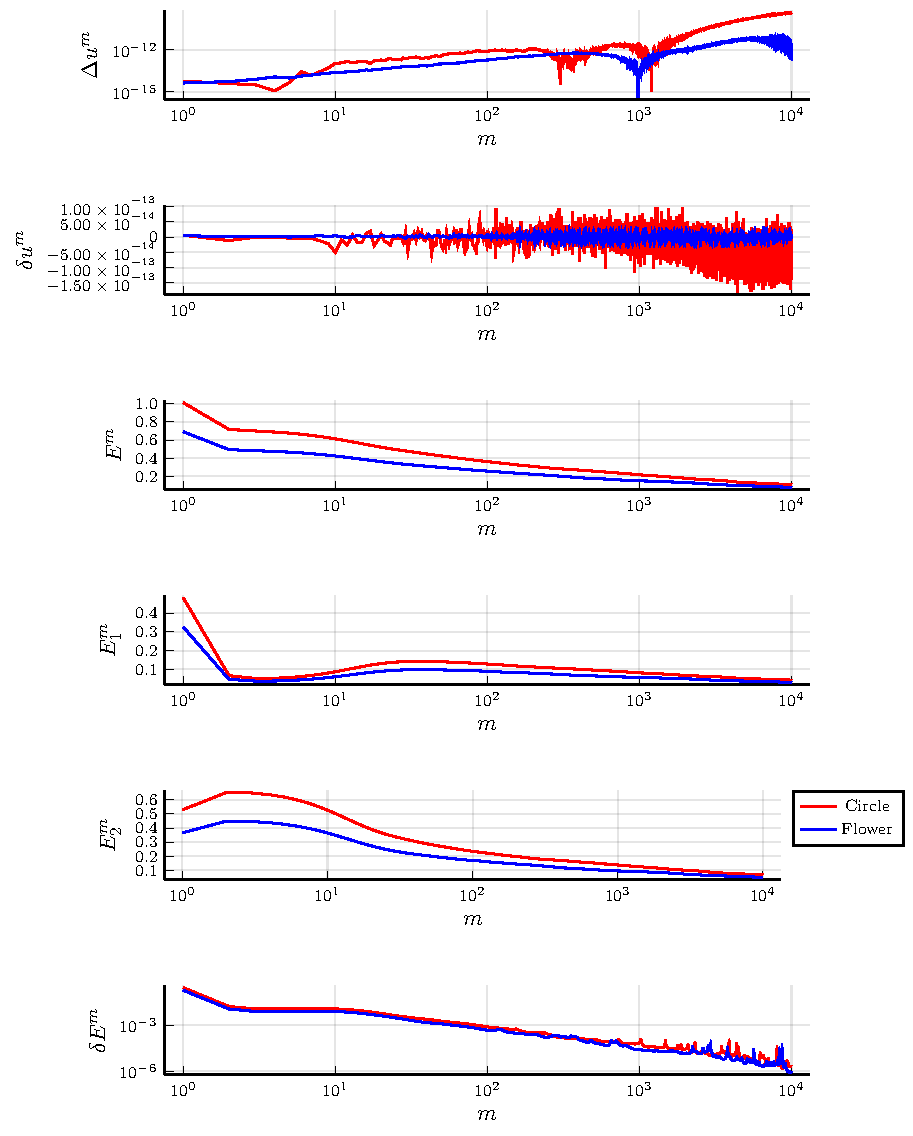
\includegraphics{results/physical_CH_plot.pdf}
\caption{Consider time as $t^{m} = m\tau $ where $m= 0,\ldots, M $, with $M = 10^4$ and timestep $\tau $. The figure describes the evolution of the relative global mass error $\Delta u^m$ and the local mass difference $\delta u^m$. It also demonstrates the total discrete energies $E^m$,$E^m_{1}$,$E^m_{2}$, along with the corresponding local energy difference $\delta E^m$. Simulations are conducted on both the circular and the flower domains.}
    \label{fig:physical_CH_plot}
\end{figure}

\begin{figure}[]
    \centering
    \hfill
    \subfloat[$m=0$]{
        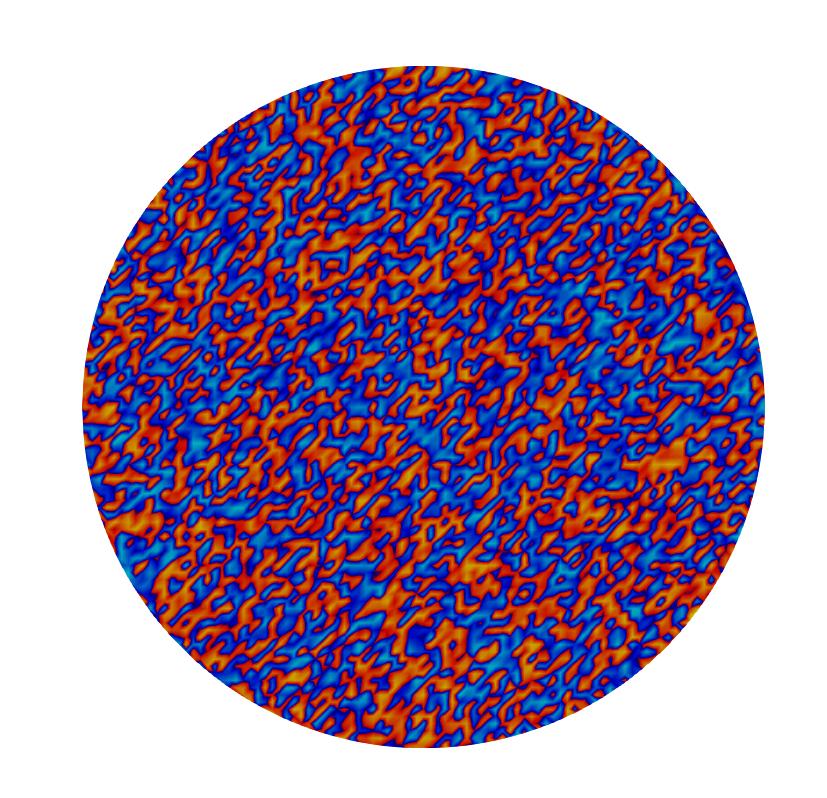
\includegraphics[width=0.3\textwidth]{results/illustration/c0.png}
    }\hfill
    \subfloat[$m=2$]{
        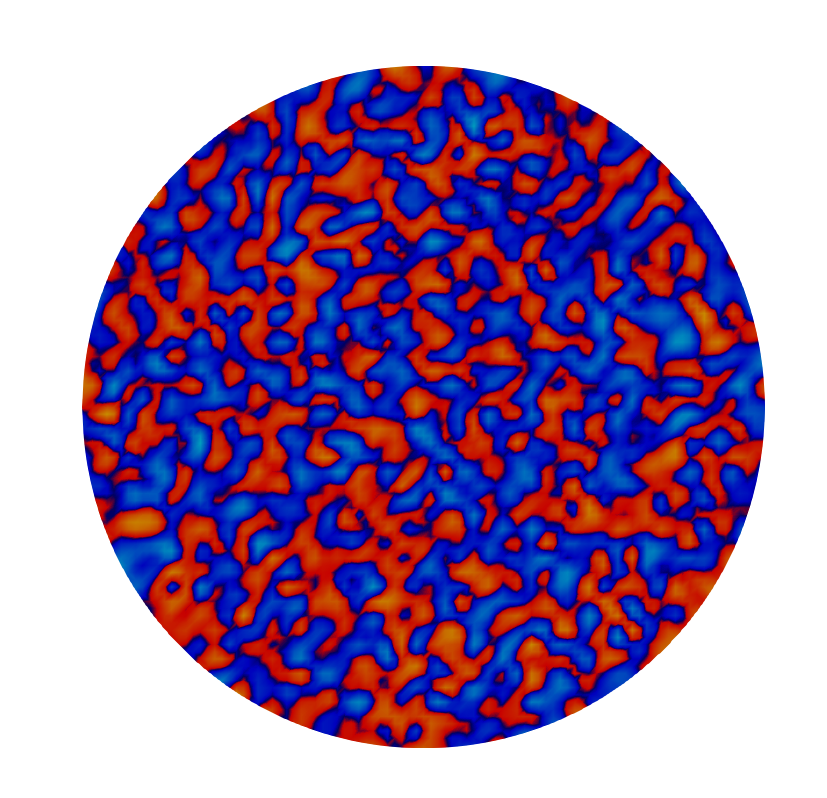
\includegraphics[width=0.3\textwidth]{results/illustration/c2.png}
    }
    \hfill
    \subfloat[$m=10$]{
        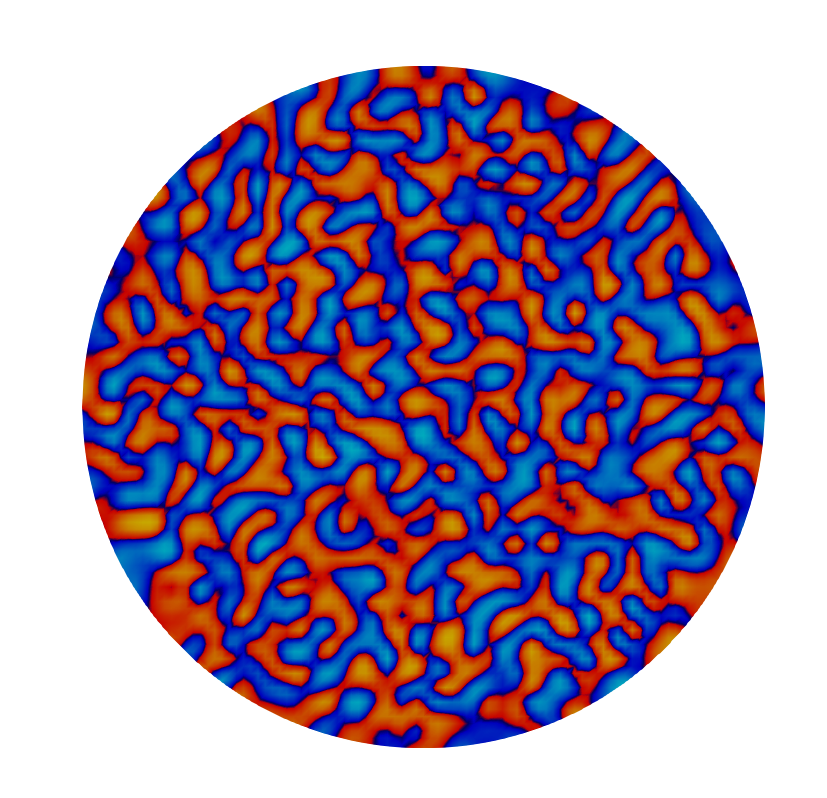
\includegraphics[width=0.3\textwidth]{results/illustration/c10.png}
    }
    \\
    \vspace{10pt}
    \hfill
    \subfloat[$m=50$]{
        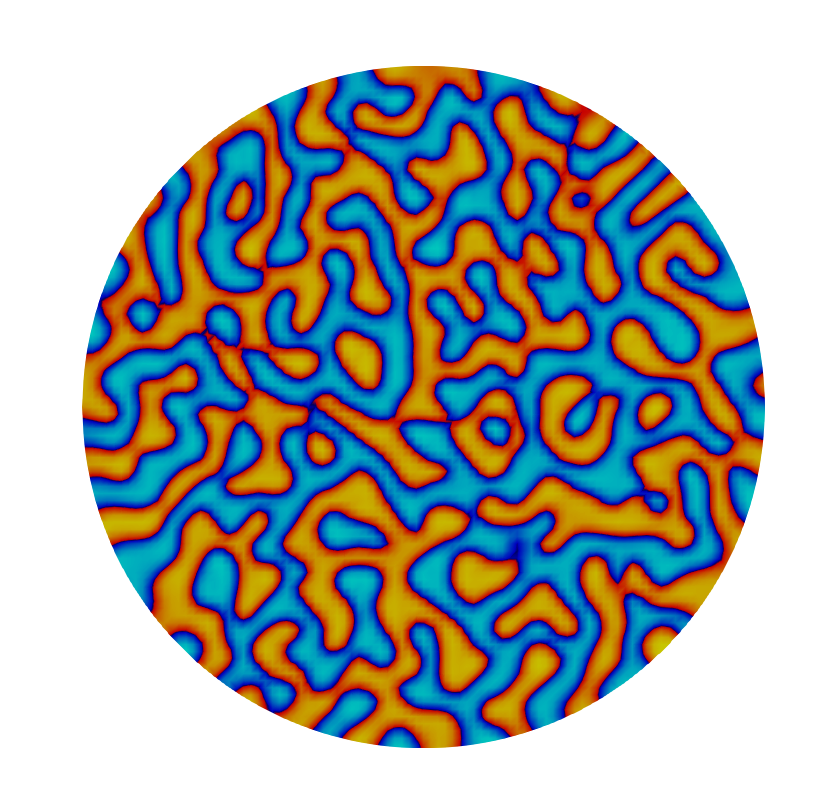
\includegraphics[width=0.3\textwidth]{results/illustration/c50.png}
    }
    \hfill
    \subfloat[$m=200$]{
        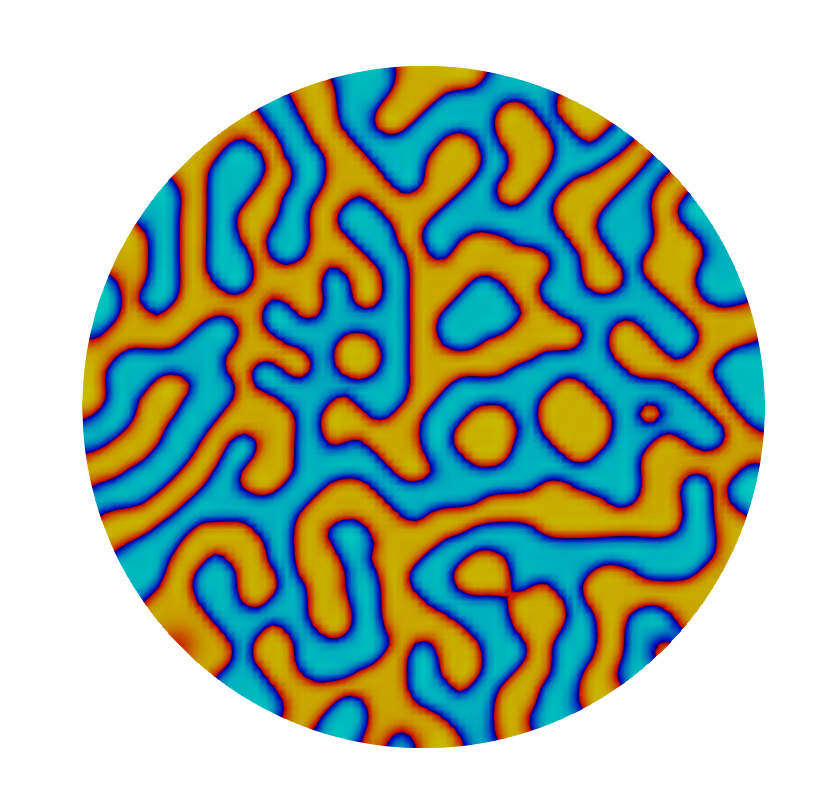
\includegraphics[width=0.3\textwidth]{results/illustration/c200.png}
    }\hfill
    \subfloat[$m=500$]{
        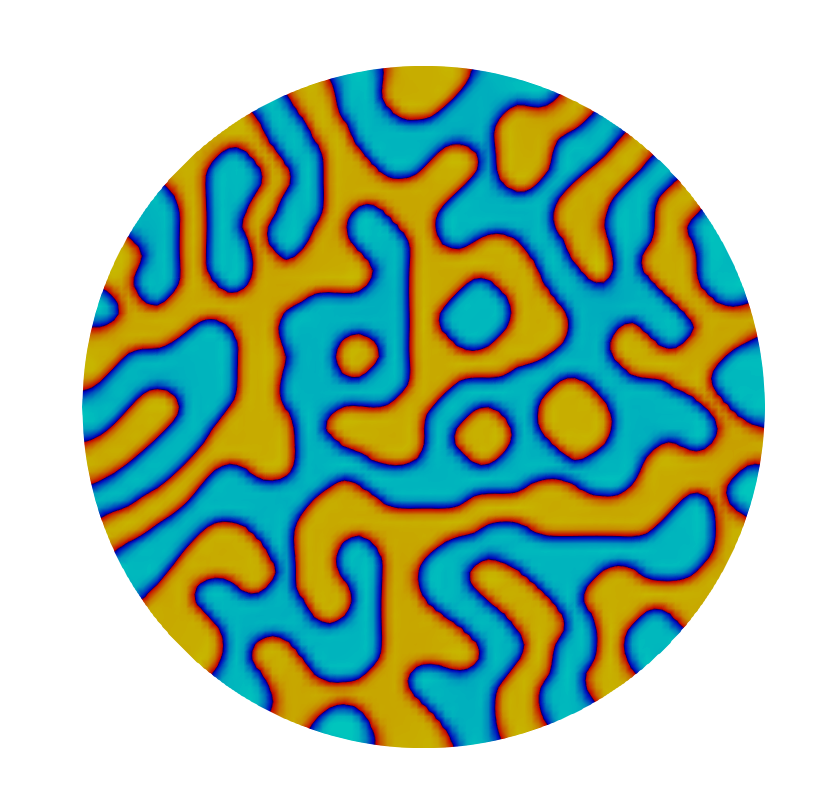
\includegraphics[width=0.3\textwidth]{results/illustration/c500.png}
    }
    \\
    \vspace{10pt}
    \hfill
    \subfloat[$m=1000$]{
        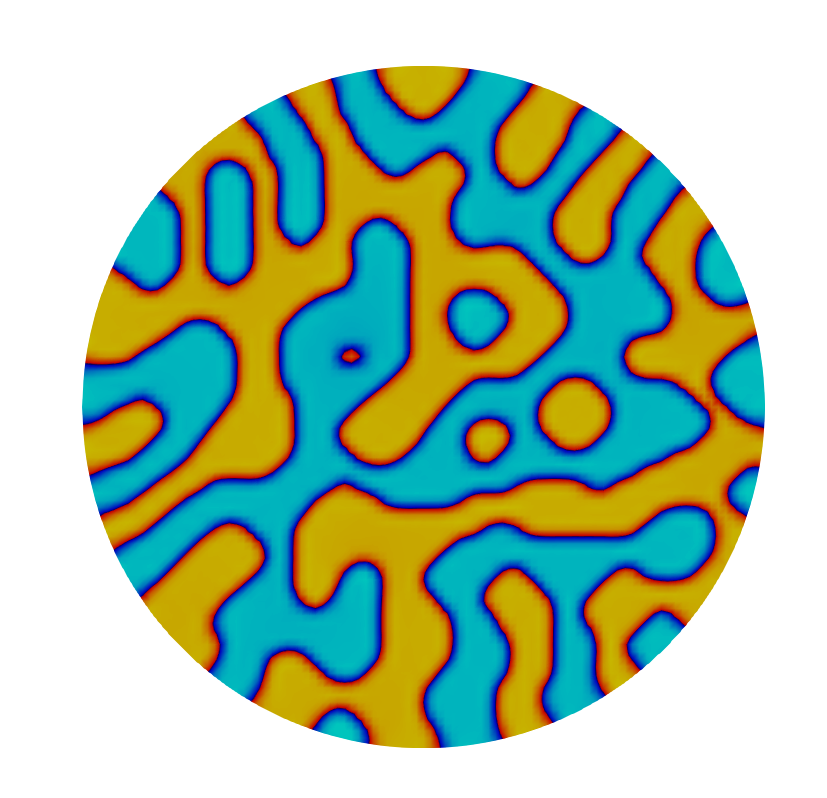
\includegraphics[width=0.3\textwidth]{results/illustration/c1000.png}
    }
    \hfill
    \subfloat[$m=5000$]{
        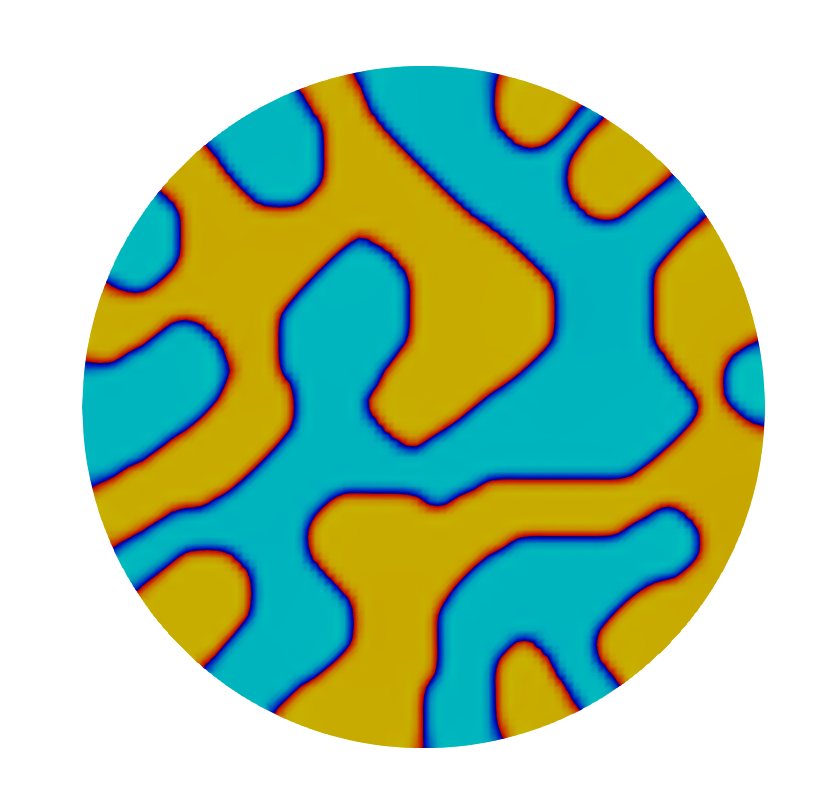
\includegraphics[width=0.3\textwidth]{results/illustration/c5000.png}
    }\hfill
    \subfloat[$m=10000$]{
        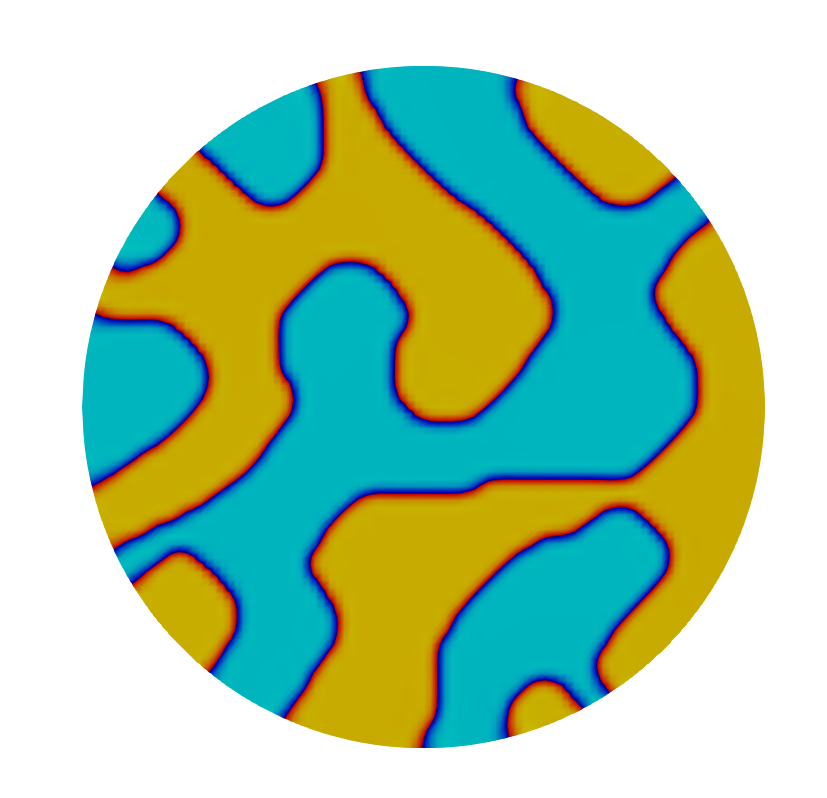
\includegraphics[width=0.3\textwidth]{results/illustration/c10000.png}
    }
    \vspace{10pt}
        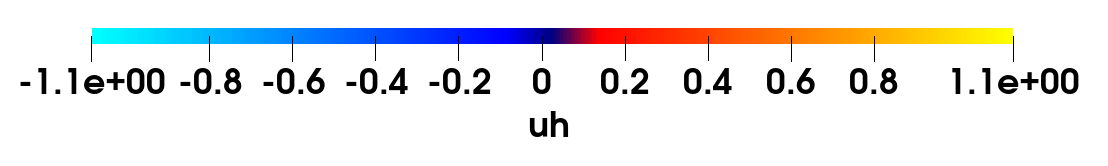
\includegraphics[width=0.8\textwidth]{results/illustration/colobar.png}

\caption{Illustration of a simulation of the Cahn-Hilliard equation on the circular domain for time $ t_{m} = m\tau $, where $\tau $ is the timestep and $m= 0,\ldots, M $, with $M = 10^4$.}
        \label{sub:fig:ill_circle}
\end{figure}

\begin{figure}[]
    \centering
    \hfill
    \subfloat[$m=0$]{
        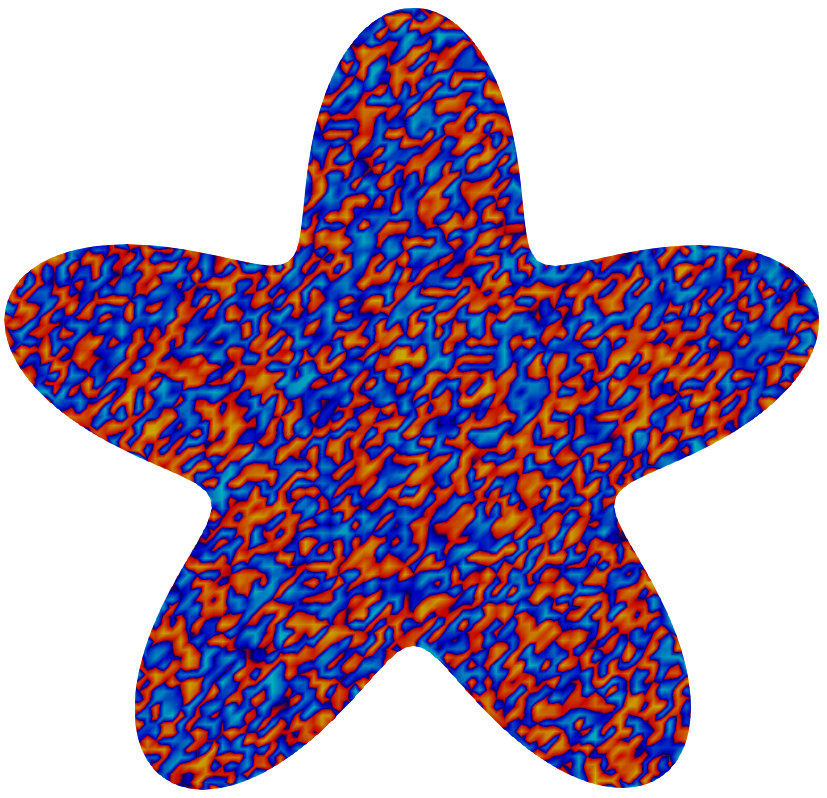
\includegraphics[width=0.3\textwidth]{results/illustration/f0.png}
    }\hfill
    \subfloat[$m=2$]{
        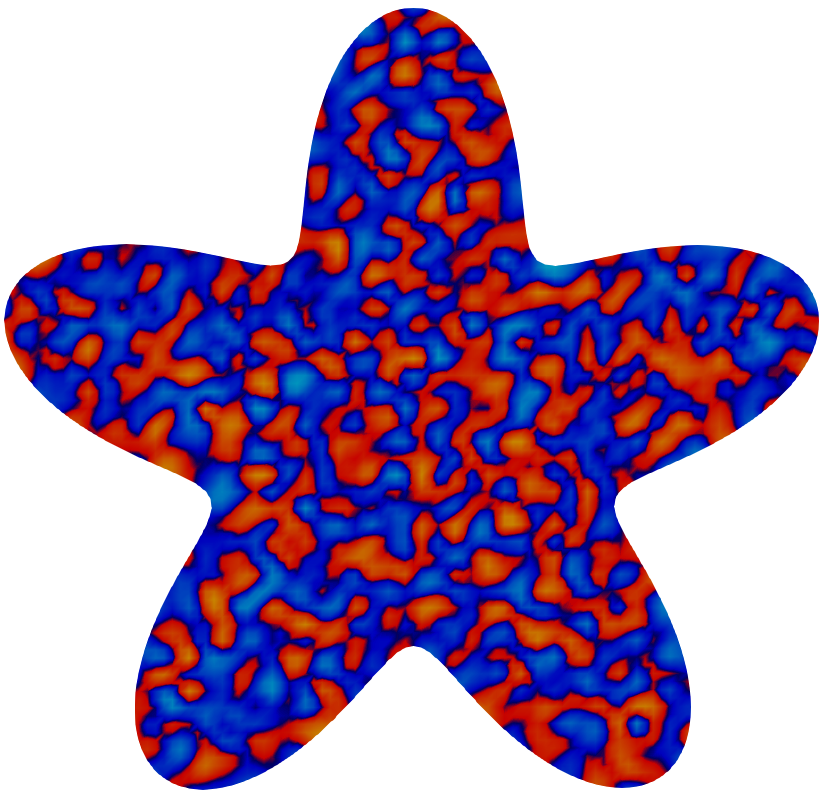
\includegraphics[width=0.3\textwidth]{results/illustration/f2.png}
    }
    \hfill
    \subfloat[$m=10$]{
        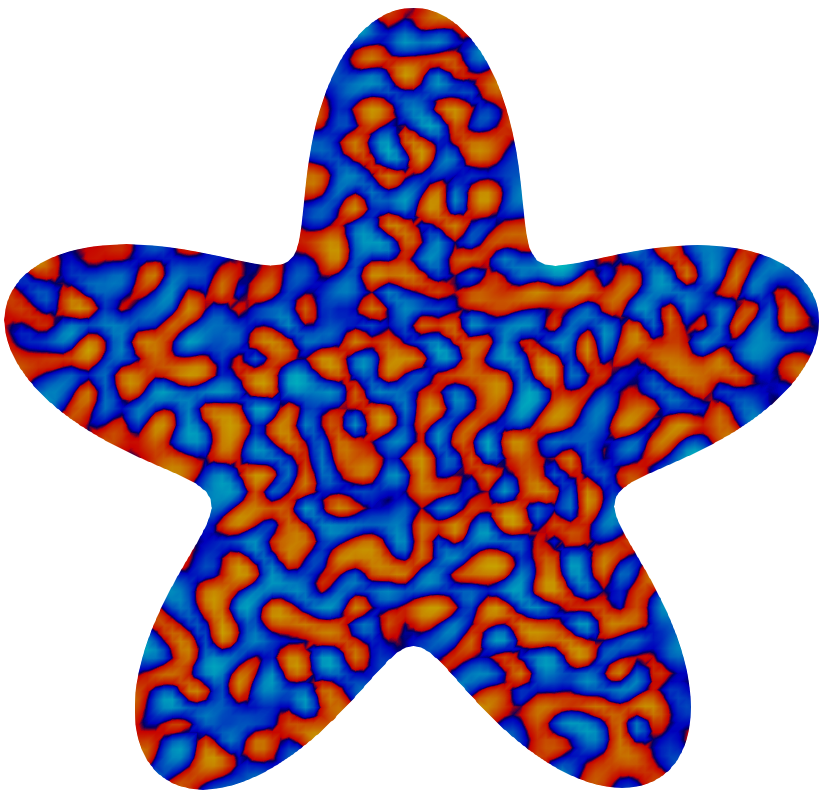
\includegraphics[width=0.3\textwidth]{results/illustration/f10.png}
    }
    \\
    \vspace{10pt}
    \hfill
    \subfloat[$m=50$]{
        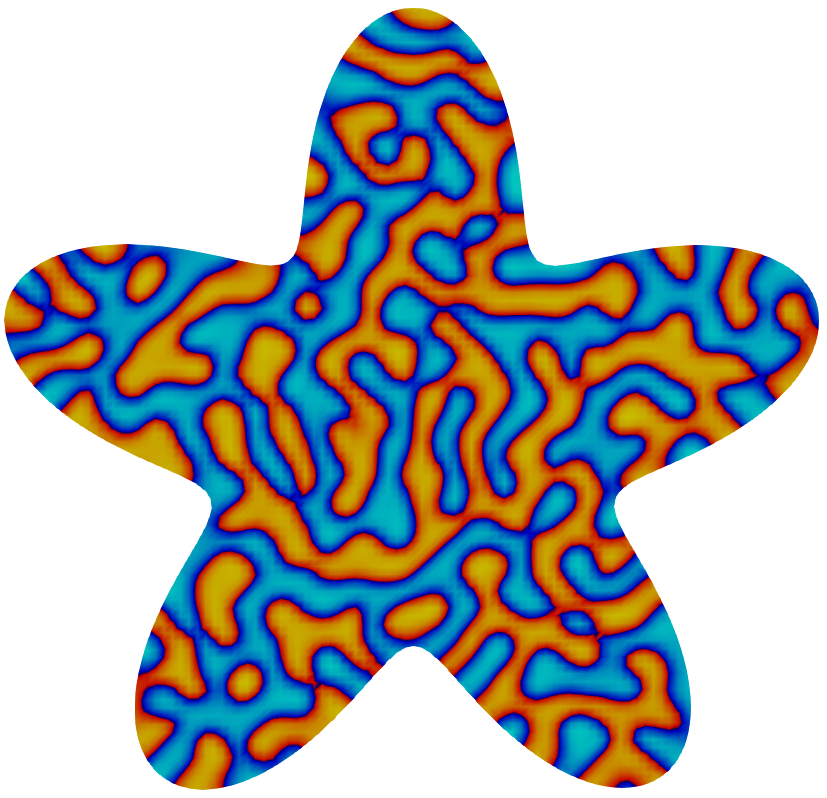
\includegraphics[width=0.3\textwidth]{results/illustration/f50.png}
    }
    \hfill
    \subfloat[$m=200$]{
        
\includegraphics[width=0.3\textwidth]{results/illustration/f200.png}
    }\hfill
    \subfloat[$m=500$]{
        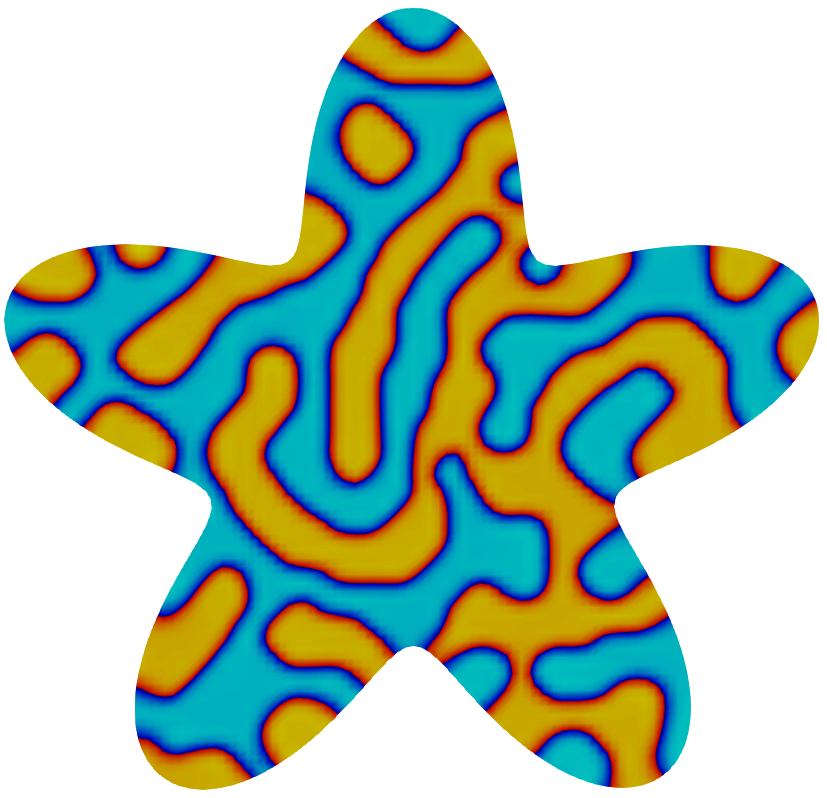
\includegraphics[width=0.3\textwidth]{results/illustration/f500.png}
    }
    \\
    \vspace{10pt}
    \hfill
    \subfloat[$m=1000$]{
        
\includegraphics[width=0.3\textwidth]{results/illustration/f1000.png}
    }
    \hfill
    \subfloat[$m=5000$]{
        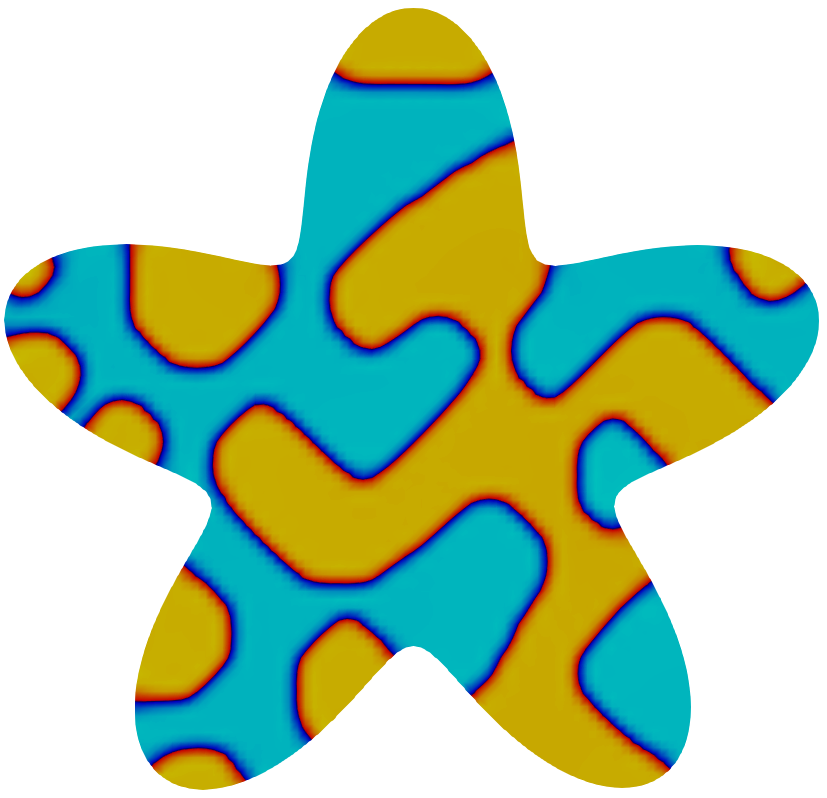
\includegraphics[width=0.3\textwidth]{results/illustration/f5000.png}
    }\hfill
    \subfloat[$m=10000$]{
        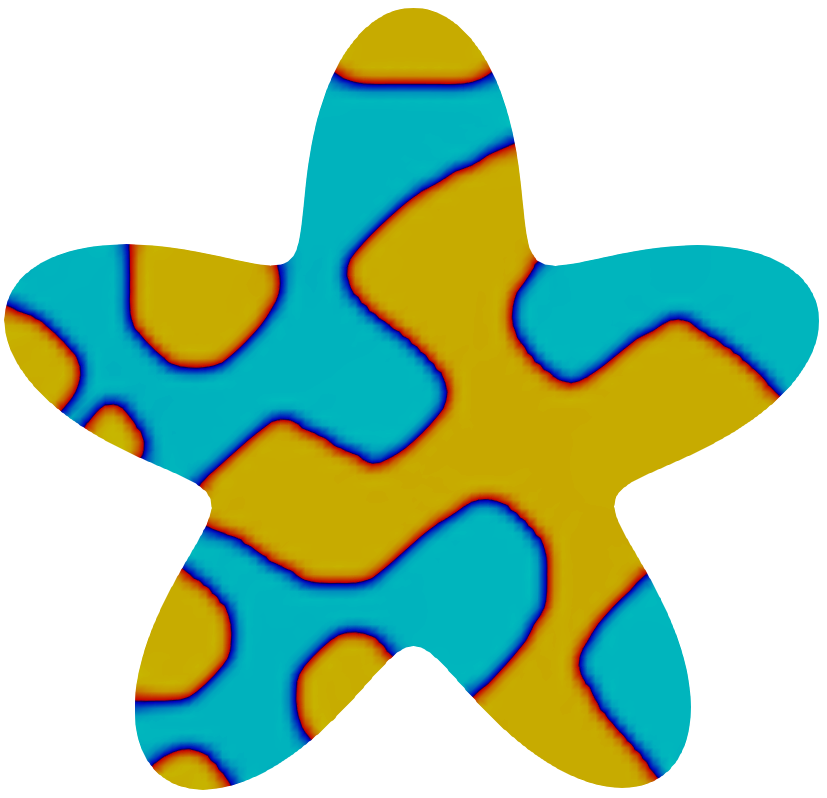
\includegraphics[width=0.3\textwidth]{results/illustration/f10000.png}
    }
    \vspace{10pt}
        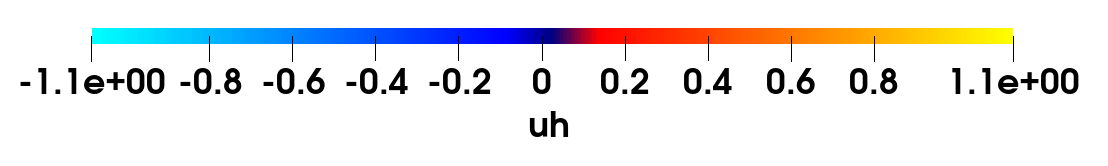
\includegraphics[width=0.8\textwidth]{results/illustration/colobar.png}
        \caption{Illustration of a simulation of the Cahn-Hilliard equation on the flower domain for time $ t_{m} = m\tau $, where $\tau $ is the timestep and $m= 0,\ldots, M $, with $M = 10^4$.}
        \label{sub:fig:ill_flower}
\end{figure}



In our experiments, we defined the initial function $u_{0}(x)$ as the uniform samples from the interval $[-1, 1]$ for each node. That is, for each node $a_{i}$, $u_{0}(a_{i})$ is a sample from the uniform distribution on the interval $[-1, 1]$. This
applies for all $i = 1, \ldots, N$, where $N$ is the total number of degrees of freedom in our system. The node $a_{i}$ is associated with the nodal basis for all $N$ degrees of freedom, as discussed for the discrete system
\eqref{eq:discretized_system}. We again used a square background mesh with length $L=2.7$ and mesh size $h=\frac{L}{n}$ for $n=2^{7}$. For an illustration of the active set $\mathcal{T}_{h} $ (defined in Section \ref{sub:unfitted_mesh}), see Figure \ref{sub:fig:active_mesh}.

\begin{figure}[H]
    \centering
    \hfill
    % \subfloat[]{
        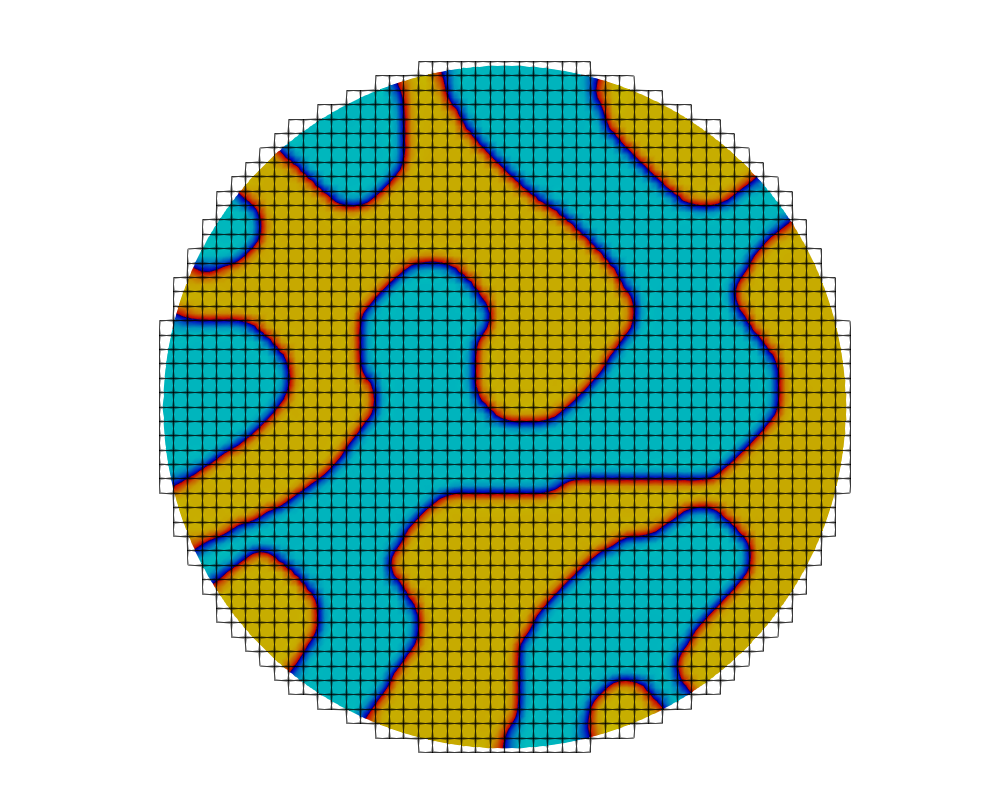
\includegraphics[width=0.45\textwidth]{results/illustration/active_circle.png}
    % }
    \hfill
    % \subfloat[]{
        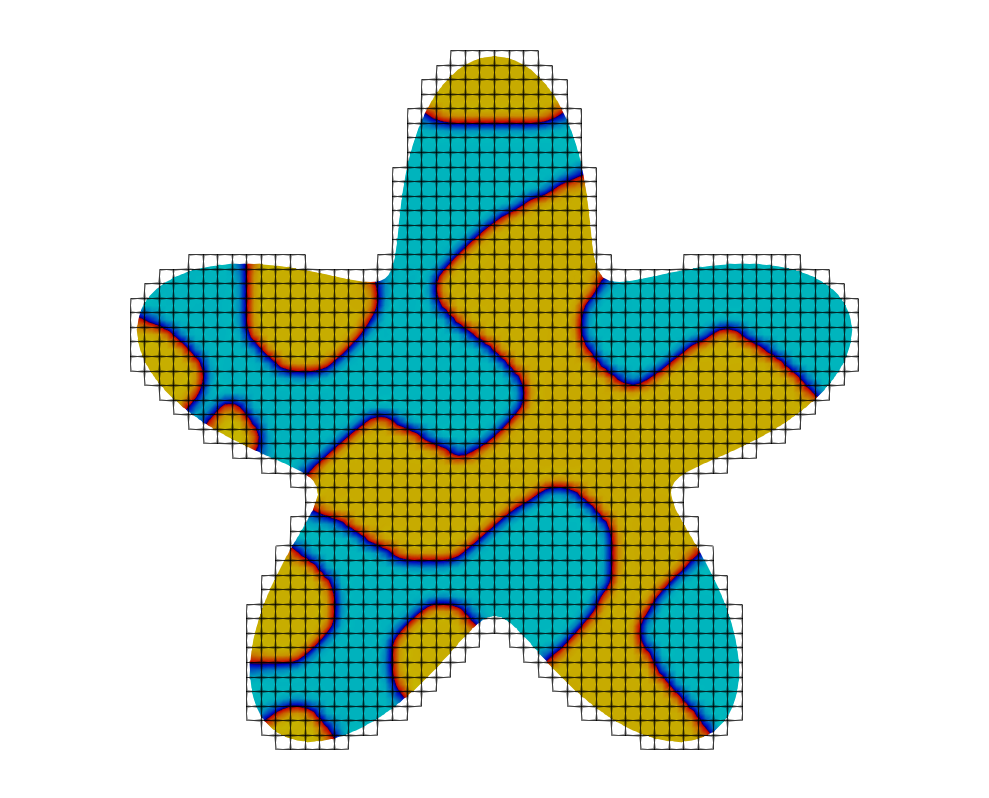
\includegraphics[width=0.45\textwidth]{results/illustration/active_flower.png}
    % }
    \caption{Illustration of the active mesh $\mathcal{T}_{h} $.}
    \label{sub:fig:active_mesh}
\end{figure}


We ran the simulation on the for the flower domain \eqref{eq:flower} and the circular domain \eqref{eq:circle}, illustrated in Figure \ref{sub:fig:ill_flower} and \ref{sub:fig:ill_circle}. The corresponding plots of the mass conservation and energy decrease are presented
in the Figure \ref{fig:physical_CH_plot}, and confirm the expected physical properties of the Cahn-Hilliard equation. The global relative error $\Delta u^{m}_{h}$ and $\delta u^{m}_{h}$ demonstrating that the mass is conserved. We also observe that the energy functional
$E(u_h)$ monotonically decreases over time and that $\delta E^{m} >0$, signifying the systems tendency to seek a state of minimal energy. Take note that $E^{m}{1}$ and $E^{m}{2}$ are interconnected in such a way that if the value of one increases, the other will correspondingly decrease to maintain balance, and vice versa.



\subsection{Note on the manufactured solution}%
\label{sub:the_problem}

While the report is not consisting of a numerical convergence analysis of the Cahn-Hilliard problem, we still present a framework for manufactured solutions for non-homogeneous boundary conditions. Let $ u( x,0) =  u_{0}$ then is Cahn-Hilliard with
non-homogeneous boundary conditions as follows,
\begin{subequations}
    \label{eq:ch_gen}
    \begin{align}
    \label{eq:ch_gen:a}
        \partial _{t} u + \Delta  \left(  \varepsilon^2  \Delta u - f( u) \right)   &= g_{0}( x)   \quad \text{ in } \Omega,  \\
        \partial _{n} u &= g_{1}( x)  \quad \text{ on } \Gamma,  \\
        \partial _{n}    \Delta u   &= g_{2}(x)  \quad \text{ on } \Gamma,
    \end{align}
\end{subequations}
where we defined $f( u) = F'( u) =u( u^2 -1)  $ for $F( u) = \frac{1}{4}( u^{2} - 1)^{2} $ and the domain $\Omega \subset \mathbb{R} ^{d} $  for $d = 2,3$. In contrast to the standard version presented in the introduction \eqref{eq:strongch}, this
version is generalized to also holds for for functions $g_{0},g_{1},g_{2}: \Omega \to\mathbb{R}   $. While the standard version may be physical correct, this version creates flexibility so we can easily construct manufactured solutions on complex domains.

    Designing a manufactured solution using $g_{0}( \cdot ) $ may be tempting with the formulation \eqref{eq:ch_gen:a}. However, observe that by expanding the Laplacian, we get
    \begin{equation}
    \begin{split}
        \Delta  \left(  \varepsilon^2  \Delta u - f( u) \right) & = \varepsilon^2 \Delta^2 u -  \Delta f( u) \\
                                                                                    &= \varepsilon^{2} \Delta ^2 u  - 3( 2u \| \nabla u \|_{ 2 }^{ 2 } + u^{2}  \Delta u )   \\
    \end{split}
    \end{equation}
Here we applied the chain rule twice and inserted the derivatives.
\begin{equation}
    \label{eq:nonlinear_laplace}
    \begin{split}
\Delta f( u)  &= \nabla \cdot \nabla f( u)  = \nabla \cdot  \left[ f' ( u) \partial _{x_{1}}u, \ldots, f' ( u) \partial _{x_{d}}u \right] ^{T} \\
& =  f'' ( u)( ( \partial _{x_{1}}u )^{2} + \ldots +( \partial _{x_{d}}u )^{2} ) +  f' ( u)( \partial _{x_{1} x_{1}}u + \ldots +   \partial _{x_{d} x_{d}}u ) \\
&=  f'' ( u) \| \nabla u \|_{ 2 }^{ 2 } + f' ( u)  \Delta u  = 6u \| \nabla u \|_{ 2 }^{ 2 } + 3u^{2}  \Delta u
    \end{split}
\end{equation}

% Our goal is to write the Cahn-Hilliard equation on weak form.
% Assume that $\Omega  \subset \mathbb{R} ^{d}$ with a $\Gamma $ in $C^2$.
%  Let $u \in  H^{4}( \Omega ) $ and $v \in V_{h} $.
% Now, expanding the first Laplace operator from a weak point of view is it clear that
% \[
%  ( \Delta ( \varepsilon  \Delta u - \frac{1}{\varepsilon } f( u) ) ,v )_{\Omega } = \varepsilon ( \Delta^{2} u ,v )_{\Omega } - \frac{1}{\varepsilon } ( \Delta f( u)  ,v )_{\Omega }.
% \]
% Hence, this makes it natural to associate the biharmonic $( \Delta ^2 u,v)_{\Omega } $ with bilinear forms $A_{h}( \cdot ,\cdot ) $ , however, in this section will we only consider the Laplace
% variant $a^{L}( \cdot ,\cdot ) $.
We now seek to find a weak form of the nonlinear term with non-homogeneous boundary conditions.
\begin{lemma}[Semi-linear form]
    Let $u \in H^4( \Omega ) $ be solution to \eqref{eq:ch_gen} and $v_{h} \in V_{h}$ the test function.
Then can we rewrite the nonlinear term into the corresponding semi-linear form $c_{h}( \cdot ,\cdot )  $ for the nonlinear term $( -\Delta f( u) , v_{h})_{\Omega }$ into two consistent formulations.
\begin{align}
    \label{eq:ch:1}
      c^{1}_{h} ( u,v_{h})  & = ( f' ( u) \nabla u, \nabla v_{h} )_{\Omega }  - ( f'( u)  g_{1}   ,  v_{h})_{\Gamma } \\
    \label{eq:ch:2}
        c^{2}_{h} ( u,v_{h})  & = -( f( u), \Delta v_{h} )_{\Omega }+  ( f( u) , \jump{ \partial _{n}v_{h} }  )_{\mathcal{F} _{h}^{int}} + ( f(u), \partial _{n} v_{h})_{\Gamma  }  - ( f'( u)  g_{1}   ,  v_{h})_{\Gamma }
\end{align}
% \begin{remark}
%     Be aware that the both formulations are consistent and if we replace $u \in H^{4}( \Omega ) $ with  $u_{h} \in  V_{h}$ we have two different discrete formulations.
% \end{remark}

\end{lemma}
% \todo[inline]{ I criticize \cite[ Remark 4.1d]{feng2007fully} which says that says that finding this weak form is not possible for conforming methods (I guess $C^{0}$ is a conforming method??). }

\begin{proof}

         \textbf{Derivation of \eqref{eq:ch:1}.  }  We want to construct the first formulation. Let $T$ be an element in $\mathcal{T}_{h}$. From the Greens theorem it is easy to see that
            \begin{equation}
            \label{eq:1_gr}
-(\Delta f( u) , v_{h})_{T } = (\nabla f( u), \nabla v_{h}  )_{T } - ( \partial _{n}  f( u), v_{h} )_{\partial T }
            \end{equation}
            First by utilizing that $\nabla f( u) = f' ( u) \nabla u $ and $\partial _{n}f( u)  = f' ( u)  \partial _{n}u$  and doing a summation over the triangles  is it clear that \[
            ( -\Delta f( u),v_{h} )_{\Omega  } =(f' ( u) \nabla u, \nabla v_{h}  )_{\Omega  } - (   f' ( u)\partial _{n}u, v_{h} )_{\partial \mathcal{T}_{h}  }
            \]
            Iterating over the facets is it clear that \[
                \begin{split}
            (   f' ( u)\partial _{n}u, v_{h} )_{\partial \mathcal{T}_{h}  } & = \sum_{F \in \mathcal{F}_{h}  }^{} \int_{F}^{}   \jump{ f' ( u)\partial _{n}u, v_{h} } \\
                                                                        & =  ( \jump{ f' ( u) \partial _{n}u },  \mean{v_{h}}    )_{\mathcal{F}^{int}_{h} } + ( \mean{ f' ( u) \partial _{n}u }, \jump{ v_{h} }    )_{\mathcal{F}^{int}_{h} } +  ( f' ( u)
                                                                        \partial _{n}u, v_{h}) _{\Gamma } \\
                                                                        & =  ( f' ( u) \partial _{n}u, v_{h}) _{\Gamma }
                \end{split}
            \]
            The jump terms vanishes by the regularity of $u$ and $v_{h}$. Hence, by inserting $g_{1}$ we have shown that the first formulation holds.

         \textbf{Derivation of \eqref{eq:ch:2}.  }  Applying an extra iteration of the Greens theorem on \eqref{eq:1_gr} we get the following terms.
\[
    \begin{split}
-(\Delta f( u) , v_{h})_{T }  = -( f( u), \Delta v_{h} )_{T} + (f( u), \partial _{n} v_{h}  )_{\partial T} - (   f'( u)\partial _{n}u, v_{h} )_{\partial T } .
    \end{split}
\]
Now, by summating all elements, it is clear that this holds.
\begin{equation}
\label{eq:f_g2}
-(\Delta f( u) , v_{h})_{\Omega  }  = -( f( u), \Delta v_{h} )_{\Omega } + (f( u), \partial _{n} v_{h}  )_{\partial \mathcal{T}_{h} } - (   f'( u)\partial _{n}u, v_{h} )_{\partial \mathcal{T}_{h}  }
\end{equation}
It comes evident from the first step of the proof that $ (   f'( u)\partial _{n}u, v_{h} )_{\partial \mathcal{T}_{h}  } = (   f'( u)\partial _{n}u, v_{h} )_{\Gamma }$, hence, we only need to compute the term $(f( u), \partial _{n} v_{h}  )_{\partial
\mathcal{T}_{h} }$ on the facets. \[
    \begin{split}
(f( u), \partial _{n} v_{h}  )_{\partial
\mathcal{T}_{h} } & = \sum_{F\in \mathcal{F} _{h}}^{} \int_{F}^{}\jump{ f( u), \partial _{n} v_{h}  } \\
& =  (\jump{ f( u)  }  , \mean{ \partial _{n} v_{h} }    )_{ \mathcal{F}_{h}^{int} } +(\mean{ f( u)  }  , \jump{ \partial _{n} v_{h} }    )_{ \mathcal{F}_{h}^{int} } + (f( u), \partial _{n} v_{h}  )_{\Gamma } \\
&=  (\mean{ f( u)  }  , \jump{ \partial _{n} v_{h} }    )_{ \mathcal{F}_{h}^{int} } + (f( u), \partial _{n} v_{h}  )_{\Gamma }
    \end{split}
\]
Again one of the jump terms vanishes because of the regularity of $u$.
Inserting the result into \eqref{eq:f_g2} we have shown that the second formulation also holds.
\end{proof}


Combining the full general Cahn-Hilliard problem in \eqref{eq:ch_gen} with the semi-linear forms\eqref{eq:ch:1} and the CutCIP biharmonic problem \eqref{eq:discrete_CutCIP_prob}, we get the following scheme.
\begin{equation}
    ( \partial _{t}u_{h}, v_{h})_\Omega + \varepsilon^2  A_{h}( u_{h},v_{h}) + c_{h}( u_{h},v_{h})   =   l_{h}(v_{h}) \quad  \forall u_{h}, v_{h} \in V_{h}
\end{equation}

To illustrate, assume we use the Laplace formulation presented in \eqref{eq:laplace_prob} integrated into \eqref{eq:discrete_CutCIP_prob}, i.e. $A_{h}( u_{h}, v_{h}) = a^{L}_{h}( u_{h}, v_{h}) + g_{h}( u_{h}, v_{h})   = l_{h}^{L}( v_{h})$. Due to the $\varepsilon $ scaling, we ultimately
arrive at the following modification.
 \begin{equation}
    l_{h}^{L}( v_{h})  =  \left( g_{0}, v_{h} \right) _{\Omega } -  \varepsilon^2 ( g_{2},  v_{h} )_{\Gamma }  -  \varepsilon^2 ( g_{1}, \Delta  v_{h}  )_{\Gamma }  + \varepsilon^2 \frac{\gamma }{h} ( g_{1}, \partial _{n} v_{h}  )_{\Gamma }
 \end{equation}
 Hence, we arrived at a system which can easily be used to construct manufactured solutions.

\newpage
\section{Conclusion}%
\label{sec:conclusion}
% First, we provided a brief overview of Sobolev spaces and basic PDE theory, introducing the
% finite element method and discussing how the error analysis is affected when our method is nonconformal, as opposed to when it is conformal.
% Next, we revisited and meticulously constructed the so-called Laplace and Hessian formulations of the continuous interior penalty methods for the biharmonic equation with Cahn-Hilliard type boundary conditions presented by \cite{brenner2012, feng2007fully}.
The primary goal of this thesis was to develop a cut finite element method for
discretizing the biharmonic problem in its primal formulation on unfitted meshes,
and to apply the resulting scheme to the Cahn-Hilliard equation.
Inspired by the theoretical discontinuous Galerkin framework for the Poisson
problem proposed in \cite{gurkan2019stabilized},
we managed to show that our method is well-posed and that the stability and convergence properties
from the original fitted formulation are maintained.
Thanks to the design of suitable ghost penalties, we could also show
that all presented theoretical properties are geometrically robust in the sense
that the derived bounds are insensitive to how the domain boundary cuts the background mesh.
The theoretical results are further substantiated by the numerical
evidence presented.  Additionally, we conducted supplementary tests to
ensure the method's geometrical robustness, particularly in instances where the
non-stabilized formulation fails.
Finally, we demonstrated that our cut continuous interior penalty
methods can successfully be applied to the nonlinear Cahn-Hilliard
equation using a simple implicit-explicit time stepping method.

While the present thesis demonstrates that the ghost penalty techniques can be successfully used
to design non-conform $C^0$-CutFEMs for elliptic
and parabolic 4th order problems, we have only scratched the surface of this research direction.
First of all, in the numerical implementation of the biharmonic problem,
we only considered elements of order $k = 2$, hence, it remains to exploit higher order, i.e. $k = 3, 4$.
In the continous interior penalty setting, as our theory already
covers the $k\geqslant 2$ case, this amounts to implement higher order
ghost penalty in our computational framework. Moreover, it would also be interesting
to compare our method to other unfitted methods, including aggregated finite element methods~\cite{BadiaVerdugoMartin2018} and
conform immersogeometric methods based on $C^1$-continuous $B$-splines~\cite{ZhaoSchillingerXu2017}.

Regarding the Cahn-Hilliard problem,
we restricted ourself to handle a constant mobility $M=1$ and a polynomial approximation of the non-linearity $F(u) =\frac{1}{4} ( u^2 - 1)^{2}$ in this report. Consequently, we need to extend and test our framework
using more physically realistic formulations, including concentration-dependent mobilities as
well as thermodynamically more relevant $\log$-based Ginzburg-Landau free energy densities $F(u)$.
From a numerical efficiency point of view, our proposed method
could significantly benefit from including adaptivity in space and time
to both resolve the locally high gradient in the phase transition zone
and to account for the different time scales in the phase separation process.
    \printbibliography

    
\includepdf[pages=-]{results/illustration/back_page.pdf}
\end{document}

